% Competition Creates Competition: the order-slot manuscript.
% pdfLaTeX. Build: latexmk -pdf -interaction=nonstopmode -halt-on-error -outdir=build main.tex
\documentclass[12pt]{article}

\usepackage[T1]{fontenc}
\usepackage[utf8]{inputenc}
\usepackage[margin=1in]{geometry}
\usepackage{amsmath,amssymb,amsthm}
\usepackage{newtxtext}
\usepackage{newtxmath}
\usepackage{microtype}
\usepackage{setspace}
\usepackage{booktabs}
\usepackage{graphicx}
\usepackage{enumitem}
\usepackage{needspace}
\usepackage[font=small,labelfont=bf,labelsep=period]{caption}
\usepackage[authoryear,round]{natbib}
\usepackage{xcolor}
\definecolor{paperlink}{RGB}{31,59,115}
\usepackage{hyperref}
\hypersetup{
  pdftitle={Competition Creates Competition: Stock Prices and the Discovery of Takeover Bidders},
  pdfauthor={Austin Li},
  colorlinks=true,
  linkcolor=paperlink,
  citecolor=paperlink,
  urlcolor=paperlink}

% Registry numbers: \reg{<key>}. Generated file; do not edit.
% numbers.tex: generated from audit/slot_manuscript_2026_10_23/registry/registry.csv.
% Do not edit by hand. Print a number with \reg{<key>}.
\makeatletter
\providecommand{\reg}[1]{\ifcsname reg@#1\endcsname\csname reg@#1\endcsname\else\textbf{??\detokenize{#1}}\PackageWarning{numbers}{Unknown registry key #1}\fi}
\expandafter\def\csname reg@B_r0_half\endcsname{1153/240}
\expandafter\def\csname reg@B_r1_half\endcsname{103/24}
\expandafter\def\csname reg@Bprior_r0\endcsname{4.804167}
\expandafter\def\csname reg@Bprior_r1_B\endcsname{4.291667}
\expandafter\def\csname reg@Bprior_r2\endcsname{4.134722}
\expandafter\def\csname reg@Delta_r0\endcsname{0.016667}
\expandafter\def\csname reg@Delta_r1\endcsname{0.666667}
\expandafter\def\csname reg@Delta_r155\endcsname{0.097581}
\expandafter\def\csname reg@Delta_r155_frac\endcsname{121/1240}
\expandafter\def\csname reg@Delta_r2\endcsname{0.938889}
\expandafter\def\csname reg@Delta_rA\endcsname{0.055670}
\expandafter\def\csname reg@J_r0\endcsname{113/18480}
\expandafter\def\csname reg@M_half_B\endcsname{0.731059}
\expandafter\def\csname reg@M_hi\endcsname{0.731392}
\expandafter\def\csname reg@M_hi_frac\endcsname{4245/5804}
\expandafter\def\csname reg@M_lo\endcsname{0.705000}
\expandafter\def\csname reg@M_lo_frac\endcsname{141/200}
\expandafter\def\csname reg@M_p5_B\endcsname{0.731059}
\expandafter\def\csname reg@M_pimax_B\endcsname{0.834698}
\expandafter\def\csname reg@QJ_r0\endcsname{4634399/15625}
\expandafter\def\csname reg@U_entry_B\endcsname{0.522757}
\expandafter\def\csname reg@U_gap_r160_B\endcsname{0.005363}
\expandafter\def\csname reg@U_mu0_B\endcsname{0.309329}
\expandafter\def\csname reg@U_sell_mu_B\endcsname{0.50}
\expandafter\def\csname reg@a236_Delta_r1_frac\endcsname{2/3}
\expandafter\def\csname reg@a236_Delta_r2_frac\endcsname{169/180}
\expandafter\def\csname reg@a236_kappa_floor_frac\endcsname{3/25}
\expandafter\def\csname reg@a236_pool_cH\endcsname{10}
\expandafter\def\csname reg@a236_pool_h\endcsname{10}
\expandafter\def\csname reg@a236_pool_k\endcsname{1/8}
\expandafter\def\csname reg@a236_pool_p\endcsname{1}
\expandafter\def\csname reg@a236_pool_perturb\endcsname{1/1000}
\expandafter\def\csname reg@a236_pool_pi1\endcsname{1/4}
\expandafter\def\csname reg@a236_pool_pi2\endcsname{1/2}
\expandafter\def\csname reg@a236_pool_pi3\endcsname{1/4}
\expandafter\def\csname reg@a236_pool_r\endcsname{8}
\expandafter\def\csname reg@a236_pool_rho\endcsname{1/4}
\expandafter\def\csname reg@a236_sig_DP0\endcsname{311/1920}
\expandafter\def\csname reg@a236_sig_DP1\endcsname{137/192}
\expandafter\def\csname reg@a236_sig_M\endcsname{8/11}
\expandafter\def\csname reg@a236_sig_alt_joint\endcsname{0.037038}
\expandafter\def\csname reg@a236_sig_alt_other\endcsname{4.171359}
\expandafter\def\csname reg@a236_sig_alt_private\endcsname{0.052500}
\expandafter\def\csname reg@a236_sig_alt_strong\endcsname{0.019067}
\expandafter\def\csname reg@a236_sig_alt_weak\endcsname{0.001455}
\expandafter\def\csname reg@a236_sig_beta\endcsname{3/10}
\expandafter\def\csname reg@a236_sig_eH\endcsname{13/16}
\expandafter\def\csname reg@a236_sig_eL\endcsname{7/16}
\expandafter\def\csname reg@a236_sig_lambda\endcsname{1/3}
\expandafter\def\csname reg@a236_sig_m\endcsname{3/11}
\expandafter\def\csname reg@a236_sig_public_cutoff\endcsname{47/106}
\expandafter\def\csname reg@a236_sig_rate0\endcsname{119/96}
\expandafter\def\csname reg@a236_sig_rate1\endcsname{4/3}
\expandafter\def\csname reg@a236_sig_sale_cutoff\endcsname{15/19}
\expandafter\def\csname reg@a236_sig_sale_floor\endcsname{19/795}
\expandafter\def\csname reg@a236_sig_sale_mu\endcsname{21/50}
\expandafter\def\csname reg@access_out_cH\endcsname{12/5}
\expandafter\def\csname reg@alt_ba_r1_B\endcsname{0.778935}
\expandafter\def\csname reg@alt_beta_B\endcsname{0.298555}
\expandafter\def\csname reg@alt_entry_r1_B\endcsname{0.522757}
\expandafter\def\csname reg@alt_lambda_B\endcsname{0.323267}
\expandafter\def\csname reg@alt_theta_B\endcsname{0.444444}
\expandafter\def\csname reg@atom_L\endcsname{1/5}
\expandafter\def\csname reg@atom_eps\endcsname{1/10}
\expandafter\def\csname reg@atom_eps_small\endcsname{1/1000}
\expandafter\def\csname reg@b0_B\endcsname{0.272648}
\expandafter\def\csname reg@b_B\endcsname{0.195615}
\expandafter\def\csname reg@b_p5_B\endcsname{0.195615}
\expandafter\def\csname reg@b_plus_lambda_B\endcsname{0.531737}
\expandafter\def\csname reg@ba_U_r155_B\endcsname{0.373656}
\expandafter\def\csname reg@ba_U_r160_B\endcsname{0.384588}
\expandafter\def\csname reg@ba_U_r165_B\endcsname{0.395776}
\expandafter\def\csname reg@ba_class_r1_B\endcsname{0.077020}
\expandafter\def\csname reg@ba_entry_r1_B\endcsname{0.709279}
\expandafter\def\csname reg@ba_jump_rC_B\endcsname{0.861835}
\expandafter\def\csname reg@ba_r1_B\endcsname{0.786299}
\expandafter\def\csname reg@ba_r2_B\endcsname{0.108469}
\expandafter\def\csname reg@ba_rC_left_B\endcsname{0.969913}
\expandafter\def\csname reg@ba_rC_right_B\endcsname{0.108078}
\expandafter\def\csname reg@ba_ratio_r1_B\endcsname{10.2}
\expandafter\def\csname reg@ba_share_r1_B\endcsname{90.2\%}
\expandafter\def\csname reg@beta_B\endcsname{0.294655}
\expandafter\def\csname reg@beta_p5_B\endcsname{0.294655}
\expandafter\def\csname reg@cH_DA_floor_B\endcsname{399/80}
\expandafter\def\csname reg@cH_afford_ceiling_B\endcsname{32/5}
\expandafter\def\csname reg@cov_entry_r1_B\endcsname{0.272757}
\expandafter\def\csname reg@cov_entry_r2_B\endcsname{0.00}
\expandafter\def\csname reg@cov_win_class_r1_B\endcsname{0.028010}
\expandafter\def\csname reg@cov_win_r1_B\endcsname{0.251863}
\expandafter\def\csname reg@cov_win_r2_B\endcsname{0.030344}
\expandafter\def\csname reg@cov_win_recruit_r1_B\endcsname{0.223853}
\expandafter\def\csname reg@d_slot_B\endcsname{0.363676}
\expandafter\def\csname reg@decisive_rmax_B\endcsname{7.968627}
\expandafter\def\csname reg@delta_rS_B\endcsname{0.297463}
\expandafter\def\csname reg@eH_r1_B\endcsname{0.648803}
\expandafter\def\csname reg@eL_r1_B\endcsname{0.396711}
\expandafter\def\csname reg@entry_cmend_B\endcsname{0.560586}
\expandafter\def\csname reg@entry_floor_obs\endcsname{0.25}
\expandafter\def\csname reg@entry_jump_B\endcsname{0.272757}
\expandafter\def\csname reg@entry_mb_r140_B\endcsname{0.459588}
\expandafter\def\csname reg@entry_mb_r145_B\endcsname{0.506112}
\expandafter\def\csname reg@entry_plateau_B\endcsname{0.522757}
\expandafter\def\csname reg@entry_r0\endcsname{0.250000}
\expandafter\def\csname reg@entry_r1_B\endcsname{0.522757}
\expandafter\def\csname reg@entry_r1_B_7\endcsname{0.5227569}
\expandafter\def\csname reg@entry_r1_unroundedbeta_7\endcsname{0.5227573}
\expandafter\def\csname reg@entry_r2\endcsname{0.250000}
\expandafter\def\csname reg@entry_r2_obs_B\endcsname{0.25}
\expandafter\def\csname reg@entry_rA_B\endcsname{0.454185}
\expandafter\def\csname reg@entry_th_r155_A\endcsname{0.350846}
\expandafter\def\csname reg@entry_th_r155_B\endcsname{0.341462}
\expandafter\def\csname reg@entry_th_r160_A\endcsname{0.328628}
\expandafter\def\csname reg@entry_th_r160_B\endcsname{0.321311}
\expandafter\def\csname reg@entry_th_r165_A\endcsname{0.310872}
\expandafter\def\csname reg@entry_th_r165_B\endcsname{0.305208}
\expandafter\def\csname reg@estar_r155\endcsname{0.580287}
\expandafter\def\csname reg@estar_r160\endcsname{0.506106}
\expandafter\def\csname reg@estar_r165\endcsname{0.447179}
\expandafter\def\csname reg@evA_r1_buy_B\endcsname{0.000000}
\expandafter\def\csname reg@evA_r1_neutral_B\endcsname{0.593750}
\expandafter\def\csname reg@evA_r1_sale_B\endcsname{0.478221}
\expandafter\def\csname reg@evA_r2_buy_B\endcsname{0.863745}
\expandafter\def\csname reg@evA_r2_neutral_B\endcsname{0.701042}
\expandafter\def\csname reg@evA_r2_sale_B\endcsname{0.538338}
\expandafter\def\csname reg@evAr_r1_neutral_B\endcsname{0.966102}
\expandafter\def\csname reg@evAr_r1_sale_B\endcsname{0.830138}
\expandafter\def\csname reg@evAr_r2_buy_B\endcsname{1.202200}
\expandafter\def\csname reg@evAr_r2_neutral_B\endcsname{1.055410}
\expandafter\def\csname reg@evAr_r2_sale_B\endcsname{0.882519}
\expandafter\def\csname reg@evN_r1_neutral_B\endcsname{-0.197917}
\expandafter\def\csname reg@evN_r1_sale_B\endcsname{-0.159407}
\expandafter\def\csname reg@evN_r2_buy_B\endcsname{-0.287915}
\expandafter\def\csname reg@evN_r2_neutral_B\endcsname{-0.233681}
\expandafter\def\csname reg@evN_r2_sale_B\endcsname{-0.179446}
\expandafter\def\csname reg@evNr_r1_neutral_B\endcsname{-0.322034}
\expandafter\def\csname reg@evNr_r1_sale_B\endcsname{-0.276713}
\expandafter\def\csname reg@evNr_r2_buy_B\endcsname{-0.400733}
\expandafter\def\csname reg@evNr_r2_neutral_B\endcsname{-0.351803}
\expandafter\def\csname reg@evNr_r2_sale_B\endcsname{-0.294173}
\expandafter\def\csname reg@evprep_mean_r1_B\endcsname{0.160592}
\expandafter\def\csname reg@evprep_mean_r2_B\endcsname{0.701042}
\expandafter\def\csname reg@evprep_meanr_r1_B\endcsname{0.270349}
\expandafter\def\csname reg@evprep_meanr_r2_B\endcsname{1.045918}
\expandafter\def\csname reg@ex_beta_M\endcsname{26/37}
\expandafter\def\csname reg@ex_beta_mu0\endcsname{41/52}
\expandafter\def\csname reg@four_prior\endcsname{1/4}
\expandafter\def\csname reg@four_v1\endcsname{1}
\expandafter\def\csname reg@four_v2\endcsname{1001/1000}
\expandafter\def\csname reg@four_v3\endcsname{9999/1000}
\expandafter\def\csname reg@four_v4\endcsname{10}
\expandafter\def\csname reg@gap_r1_rS_B\endcsname{0.875852}
\expandafter\def\csname reg@gap_r2_rC_B\endcsname{0.007341}
\expandafter\def\csname reg@gap_rA_r0_B\endcsname{0.193958}
\expandafter\def\csname reg@gap_rC_r1_B\endcsname{0.592659}
\expandafter\def\csname reg@gap_rF_rA_B\endcsname{0.073169}
\expandafter\def\csname reg@gap_rJ_rN_B\endcsname{0.218220}
\expandafter\def\csname reg@gap_rN_rF_B\endcsname{0.280750}
\expandafter\def\csname reg@gap_rS_rJ_B\endcsname{0.158051}
\expandafter\def\csname reg@imb_buy_B\endcsname{0.168061}
\expandafter\def\csname reg@impact_asym_r1_B\endcsname{0.709279}
\expandafter\def\csname reg@impact_buy_r1_B\endcsname{0.747789}
\expandafter\def\csname reg@impact_sell_r1_B\endcsname{0.038510}
\expandafter\def\csname reg@impact_sell_r2_B\endcsname{0.054235}
\expandafter\def\csname reg@lambda_B\endcsname{0.336122}
\expandafter\def\csname reg@lambda_hi_B\endcsname{0.336721}
\expandafter\def\csname reg@lambda_hi_third\endcsname{0.364797}
\expandafter\def\csname reg@lambda_lo_B\endcsname{0.290539}
\expandafter\def\csname reg@lambda_lo_third\endcsname{0.316602}
\expandafter\def\csname reg@lambda_p5_B\endcsname{0.336122}
\expandafter\def\csname reg@lap_A6_strong_entry_margin\endcsname{0.117155}
\expandafter\def\csname reg@lap_Delta_r0\endcsname{0.016667}
\expandafter\def\csname reg@lap_Delta_r1\endcsname{0.666667}
\expandafter\def\csname reg@lap_Delta_r2\endcsname{0.938889}
\expandafter\def\csname reg@lap_M_half\endcsname{0.731059}
\expandafter\def\csname reg@lap_P3_GammaH_r155\endcsname{\ensuremath{7.6\times10^{-5}}}
\expandafter\def\csname reg@lap_P3_GammaH_r160\endcsname{0.002753}
\expandafter\def\csname reg@lap_P3_GammaH_r165\endcsname{0.005492}
\expandafter\def\csname reg@lap_P3_entry_r155\endcsname{0.545053}
\expandafter\def\csname reg@lap_P3_entry_r160\endcsname{0.548756}
\expandafter\def\csname reg@lap_P3_entry_r165\endcsname{0.551361}
\expandafter\def\csname reg@lap_P3_pool_r155\endcsname{0.007802}
\expandafter\def\csname reg@lap_P3_pool_r160\endcsname{0.005938}
\expandafter\def\csname reg@lap_P3_pool_r165\endcsname{0.003996}
\expandafter\def\csname reg@lap_P3_psi_left_r155\endcsname{\ensuremath{1.1\times10^{-10}}}
\expandafter\def\csname reg@lap_P3_psi_right_r155\endcsname{\ensuremath{-9.6\times10^{-11}}}
\expandafter\def\csname reg@lap_P3_thr_r155\endcsname{0.028042}
\expandafter\def\csname reg@lap_P3_v_r155\endcsname{0.460316}
\expandafter\def\csname reg@lap_P3_v_r160\endcsname{0.707475}
\expandafter\def\csname reg@lap_P3_v_r165\endcsname{0.903332}
\expandafter\def\csname reg@lap_access_proceeds_gain\endcsname{0.257809}
\expandafter\def\csname reg@lap_access_surplus\endcsname{2.632301}
\expandafter\def\csname reg@lap_access_surplus_gain\endcsname{0.080218}
\expandafter\def\csname reg@lap_b\endcsname{2}
\expandafter\def\csname reg@lap_break_even_scale\endcsname{1.831923}
\expandafter\def\csname reg@lap_cH_hi\endcsname{6.217155}
\expandafter\def\csname reg@lap_cH_lo\endcsname{5.997311}
\expandafter\def\csname reg@lap_caseA_entry_r1\endcsname{0.464564}
\expandafter\def\csname reg@lap_caseB_entry_r1\endcsname{0.571808}
\expandafter\def\csname reg@lap_caseC_entry_r1\endcsname{0.563404}
\expandafter\def\csname reg@lap_caseD_A1_upper\endcsname{-0.018122}
\expandafter\def\csname reg@lap_entry_r1\endcsname{0.522757}
\expandafter\def\csname reg@lap_frozen_r0_entry\endcsname{0.562178}
\expandafter\def\csname reg@lap_frozen_r1_entry\endcsname{0.522757}
\expandafter\def\csname reg@lap_gH_r2\endcsname{5879/720}
\expandafter\def\csname reg@lap_gL_r2\endcsname{5/48}
\expandafter\def\csname reg@lap_gross_profit_unit\endcsname{0.140731}
\expandafter\def\csname reg@lap_hidden_surplus\endcsname{2.552083}
\expandafter\def\csname reg@lap_logistic_entry\endcsname{0.301509}
\expandafter\def\csname reg@lap_m_half\endcsname{0.268941}
\expandafter\def\csname reg@lap_margin_A1_lower\endcsname{1.195833}
\expandafter\def\csname reg@lap_margin_A1_upper\endcsname{0.217155}
\expandafter\def\csname reg@lap_margin_A2_lower\endcsname{0.003333}
\expandafter\def\csname reg@lap_margin_A2_upper\endcsname{0.002412}
\expandafter\def\csname reg@lap_margin_ownership\endcsname{3/4}
\expandafter\def\csname reg@lap_mixture_entry_r1\endcsname{0.522715}
\expandafter\def\csname reg@lap_moderate_A2_upper\endcsname{0.000801}
\expandafter\def\csname reg@lap_moderate_entry_r1\endcsname{0.526805}
\expandafter\def\csname reg@lap_own_r1\endcsname{0.324192}
\expandafter\def\csname reg@lap_prior_hi\endcsname{0.500424}
\expandafter\def\csname reg@lap_prior_ii_hi\endcsname{0.538096}
\expandafter\def\csname reg@lap_prior_lo\endcsname{0.467850}
\expandafter\def\csname reg@lap_r2_minus_rC\endcsname{0.007341}
\expandafter\def\csname reg@lap_rC\endcsname{3.592659}
\expandafter\def\csname reg@lap_rN\endcsname{1.747878}
\expandafter\def\csname reg@lap_rU\endcsname{2.837417}
\expandafter\def\csname reg@lap_r_unique_zero\endcsname{1.220998}
\expandafter\def\csname reg@lap_reserve_excl_p\endcsname{1.01}
\expandafter\def\csname reg@lap_reserve_excl_r0_entry\endcsname{0.543573}
\expandafter\def\csname reg@lap_reserve_excl_r1_entry\endcsname{0.513373}
\expandafter\def\csname reg@lap_return_cost\endcsname{0.002689}
\expandafter\def\csname reg@lap_return_post\endcsname{0.000334}
\expandafter\def\csname reg@lap_return_trade\endcsname{0.011563}
\expandafter\def\csname reg@lap_signal_entry_r0\endcsname{0.850000}
\expandafter\def\csname reg@lap_signal_entry_r1\endcsname{0.879438}
\expandafter\def\csname reg@lap_spread_increase\endcsname{0.272222}
\expandafter\def\csname reg@lap_stake_omegaU\endcsname{0.011434}
\expandafter\def\csname reg@lap_tau_r0\endcsname{0.633117}
\expandafter\def\csname reg@lap_tau_r1\endcsname{0.705000}
\expandafter\def\csname reg@lap_tau_r2\endcsname{0.731392}
\expandafter\def\csname reg@lap_xstar_r1\endcsname{0.871222}
\expandafter\def\csname reg@m_half_B\endcsname{0.268941}
\expandafter\def\csname reg@m_p5_B\endcsname{0.268941}
\expandafter\def\csname reg@margin_Delta_pos_B\endcsname{0.016667}
\expandafter\def\csname reg@margin_Delta_pos_B_frac\endcsname{1/60}
\expandafter\def\csname reg@margin_J_r0_B\endcsname{0.013885}
\expandafter\def\csname reg@margin_J_r0_B_frac\endcsname{1283/92400}
\expandafter\def\csname reg@margin_balance_B\endcsname{1.167512}
\expandafter\def\csname reg@margin_balance_B_frac\endcsname{9667/8280}
\expandafter\def\csname reg@margin_balance_sq_B\endcsname{0.169746}
\expandafter\def\csname reg@margin_balance_sq_B_frac\endcsname{937/5520}
\expandafter\def\csname reg@margin_beta_B\endcsname{0.038678}
\expandafter\def\csname reg@margin_cmend_B\endcsname{0.000343}
\expandafter\def\csname reg@margin_decisive_B_frac\endcsname{81/80}
\expandafter\def\csname reg@margin_decisive_rmax_B\endcsname{2.031373}
\expandafter\def\csname reg@margin_gHgL_B\endcsname{8.061111}
\expandafter\def\csname reg@margin_gHgL_B_frac\endcsname{1451/180}
\expandafter\def\csname reg@margin_implied_prior_r1\endcsname{1.708333}
\expandafter\def\csname reg@margin_implied_prior_r2\endcsname{1.865278}
\expandafter\def\csname reg@margin_kstrong2_B\endcsname{0.043127}
\expandafter\def\csname reg@margin_kstrong_B\endcsname{0.024824}
\expandafter\def\csname reg@margin_kstrong_r2pt0_B\endcsname{-0.003191}
\expandafter\def\csname reg@margin_kweak_B\endcsname{0.003333}
\expandafter\def\csname reg@margin_lambda_hi_B\endcsname{0.000599}
\expandafter\def\csname reg@margin_lambda_lo_B\endcsname{0.045583}
\expandafter\def\csname reg@margin_obs_band_incentive_B\endcsname{0.024768}
\expandafter\def\csname reg@margin_obs_beta_B\endcsname{0.038678}
\expandafter\def\csname reg@margin_obs_buy_r155_B\endcsname{0.006243}
\expandafter\def\csname reg@margin_obs_buy_recruit_B\endcsname{0.026059}
\expandafter\def\csname reg@margin_obs_buy_recruit_r165_B\endcsname{0.713202}
\expandafter\def\csname reg@margin_obs_ceiling_B\endcsname{0.000334}
\expandafter\def\csname reg@margin_obs_full_orders_r1_B\endcsname{0.024824}
\expandafter\def\csname reg@margin_obs_full_orders_r2_B\endcsname{0.043127}
\expandafter\def\csname reg@margin_obs_lowsell_r165_B\endcsname{0.003996}
\expandafter\def\csname reg@margin_obs_neutral_r1_B\endcsname{1.708333}
\expandafter\def\csname reg@margin_obs_post_over_58_B\endcsname{0.106059}
\expandafter\def\csname reg@margin_obs_r2_above_rC_B\endcsname{0.007341}
\expandafter\def\csname reg@margin_obs_rF_B\endcsname{0.082873}
\expandafter\def\csname reg@margin_obs_rN_B\endcsname{0.097878}
\expandafter\def\csname reg@margin_obs_rN_rC_B\endcsname{1.844781}
\expandafter\def\csname reg@margin_obs_rS_h_B\endcsname{7.875852}
\expandafter\def\csname reg@margin_obs_rS_rC_B\endcsname{1.468510}
\expandafter\def\csname reg@margin_obs_u_hi_B\endcsname{0.004617}
\expandafter\def\csname reg@margin_obs_u_lo_B\endcsname{0.328451}
\expandafter\def\csname reg@margin_obs_weak_r0_B\endcsname{0.003333}
\expandafter\def\csname reg@margin_p2_bands_collapse_B\endcsname{0.002658}
\expandafter\def\csname reg@margin_p2_bands_collapse_high_B\endcsname{0.043134}
\expandafter\def\csname reg@margin_p2_bands_collapse_low_B\endcsname{0.043134}
\expandafter\def\csname reg@margin_p2_bands_high_floor_B\endcsname{0.024833}
\expandafter\def\csname reg@margin_p2_bands_low_floor_B\endcsname{0.024833}
\expandafter\def\csname reg@margin_p2_bands_ownership_B\endcsname{0.398803}
\expandafter\def\csname reg@margin_p2_bands_strong_prior_B\endcsname{1.708264}
\expandafter\def\csname reg@margin_p2_bands_strong_top_B\endcsname{0.217192}
\expandafter\def\csname reg@margin_p2_bands_weak_cost_B\endcsname{1.195660}
\expandafter\def\csname reg@margin_p2_bands_weak_trade_B\endcsname{0.002986}
\expandafter\def\csname reg@margin_p2_base_collapse_B\endcsname{0.002689}
\expandafter\def\csname reg@margin_p2_base_collapse_high_B\endcsname{0.043127}
\expandafter\def\csname reg@margin_p2_base_collapse_low_B\endcsname{0.043127}
\expandafter\def\csname reg@margin_p2_base_high_floor_B\endcsname{0.024824}
\expandafter\def\csname reg@margin_p2_base_low_floor_B\endcsname{0.024824}
\expandafter\def\csname reg@margin_p2_base_ownership_B\endcsname{0.398803}
\expandafter\def\csname reg@margin_p2_base_strong_prior_B\endcsname{1.708333}
\expandafter\def\csname reg@margin_p2_base_strong_top_B\endcsname{0.217155}
\expandafter\def\csname reg@margin_p2_base_weak_cost_B\endcsname{1.195833}
\expandafter\def\csname reg@margin_p2_base_weak_trade_B\endcsname{0.003333}
\expandafter\def\csname reg@margin_p2_beta_lower_B\endcsname{0.294655}
\expandafter\def\csname reg@margin_p2_beta_upper_B\endcsname{0.038678}
\expandafter\def\csname reg@margin_p2_bplus_B\endcsname{0.031737}
\expandafter\def\csname reg@margin_p2_deter_lower_B\endcsname{0.224730}
\expandafter\def\csname reg@margin_p2_deter_upper_B\endcsname{0.242723}
\expandafter\def\csname reg@margin_p2_ex_a_collapse_B\endcsname{0.058137}
\expandafter\def\csname reg@margin_p2_ex_a_collapse_high_B\endcsname{0.098418}
\expandafter\def\csname reg@margin_p2_ex_a_collapse_low_B\endcsname{0.021967}
\expandafter\def\csname reg@margin_p2_ex_a_high_floor_B\endcsname{0.066983}
\expandafter\def\csname reg@margin_p2_ex_a_low_floor_B\endcsname{0.012698}
\expandafter\def\csname reg@margin_p2_ex_a_ownership_B\endcsname{0.398803}
\expandafter\def\csname reg@margin_p2_ex_a_strong_prior_B\endcsname{1.875000}
\expandafter\def\csname reg@margin_p2_ex_a_strong_top_B\endcsname{0.109179}
\expandafter\def\csname reg@margin_p2_ex_a_weak_cost_B\endcsname{1.460455}
\expandafter\def\csname reg@margin_p2_ex_a_weak_trade_B\endcsname{0.005455}
\expandafter\def\csname reg@margin_p2_ex_b_collapse_B\endcsname{0.132569}
\expandafter\def\csname reg@margin_p2_ex_b_collapse_high_B\endcsname{0.021967}
\expandafter\def\csname reg@margin_p2_ex_b_collapse_low_B\endcsname{0.098418}
\expandafter\def\csname reg@margin_p2_ex_b_high_floor_B\endcsname{0.012698}
\expandafter\def\csname reg@margin_p2_ex_b_low_floor_B\endcsname{0.066983}
\expandafter\def\csname reg@margin_p2_ex_b_ownership_B\endcsname{0.398803}
\expandafter\def\csname reg@margin_p2_ex_b_strong_prior_B\endcsname{1.241667}
\expandafter\def\csname reg@margin_p2_ex_b_strong_top_B\endcsname{0.123413}
\expandafter\def\csname reg@margin_p2_ex_b_weak_cost_B\endcsname{0.562273}
\expandafter\def\csname reg@margin_p2_ex_b_weak_trade_B\endcsname{0.005455}
\expandafter\def\csname reg@margin_p2_ex_c_collapse_B\endcsname{0.314551}
\expandafter\def\csname reg@margin_p2_ex_c_collapse_high_B\endcsname{0.037620}
\expandafter\def\csname reg@margin_p2_ex_c_collapse_low_B\endcsname{0.175423}
\expandafter\def\csname reg@margin_p2_ex_c_high_floor_B\endcsname{0.023541}
\expandafter\def\csname reg@margin_p2_ex_c_low_floor_B\endcsname{0.127671}
\expandafter\def\csname reg@margin_p2_ex_c_ownership_B\endcsname{0.349742}
\expandafter\def\csname reg@margin_p2_ex_c_strong_prior_B\endcsname{1.205913}
\expandafter\def\csname reg@margin_p2_ex_c_strong_top_B\endcsname{0.058891}
\expandafter\def\csname reg@margin_p2_ex_c_weak_cost_B\endcsname{0.021000}
\expandafter\def\csname reg@margin_p2_ex_c_weak_trade_B\endcsname{0.006667}
\expandafter\def\csname reg@margin_p2_ex_d_collapse_B\endcsname{0.447727}
\expandafter\def\csname reg@margin_p2_ex_d_collapse_high_B\endcsname{0.042679}
\expandafter\def\csname reg@margin_p2_ex_d_collapse_low_B\endcsname{0.192578}
\expandafter\def\csname reg@margin_p2_ex_d_high_floor_B\endcsname{0.026343}
\expandafter\def\csname reg@margin_p2_ex_d_low_floor_B\endcsname{0.137174}
\expandafter\def\csname reg@margin_p2_ex_d_ownership_B\endcsname{0.398803}
\expandafter\def\csname reg@margin_p2_ex_d_strong_prior_B\endcsname{1.269444}
\expandafter\def\csname reg@margin_p2_ex_d_strong_top_B\endcsname{-0.018122}
\expandafter\def\csname reg@margin_p2_ex_d_weak_cost_B\endcsname{0.025000}
\expandafter\def\csname reg@margin_p2_ex_d_weak_trade_B\endcsname{0.020000}
\expandafter\def\csname reg@margin_p2_lambda_lower_B\endcsname{0.336122}
\expandafter\def\csname reg@margin_p2_lambda_upper_B\endcsname{0.663878}
\expandafter\def\csname reg@margin_p2_many_beta_B\endcsname{0.044655}
\expandafter\def\csname reg@margin_p2_many_w_lower_B\endcsname{0.940709}
\expandafter\def\csname reg@margin_p2_many_w_upper_B\endcsname{0.059291}
\expandafter\def\csname reg@margin_p2_moderate_high_floor_B\endcsname{0.003603}
\expandafter\def\csname reg@margin_p2_moderate_low_floor_B\endcsname{0.003603}
\expandafter\def\csname reg@margin_p2_moderate_ownership_B\endcsname{0.398803}
\expandafter\def\csname reg@margin_p2_moderate_strong_prior_B\endcsname{0.181667}
\expandafter\def\csname reg@margin_p2_moderate_strong_top_B\endcsname{0.030137}
\expandafter\def\csname reg@margin_p2_moderate_weak_cost_B\endcsname{0.033452}
\expandafter\def\csname reg@margin_p2_moderate_weak_trade_B\endcsname{0.000810}
\expandafter\def\csname reg@margin_p2_ph_prior_B\endcsname{1.896362}
\expandafter\def\csname reg@margin_p2_ph_trade_B\endcsname{0.050792}
\expandafter\def\csname reg@margin_p2_ph_weak_B\endcsname{0.125270}
\expandafter\def\csname reg@margin_p2_posterior_collapse_B\endcsname{0.000334}
\expandafter\def\csname reg@margin_p2_primitive_class_gap_B\endcsname{9.000000}
\expandafter\def\csname reg@margin_p2_primitive_cost_B\endcsname{6.000000}
\expandafter\def\csname reg@margin_p2_primitive_high_above_r2_B\endcsname{6.400000}
\expandafter\def\csname reg@margin_p2_primitive_k_B\endcsname{0.020000}
\expandafter\def\csname reg@margin_p2_primitive_low_above_p_B\endcsname{0.500000}
\expandafter\def\csname reg@margin_p2_primitive_one_minus_pi_B\endcsname{0.500000}
\expandafter\def\csname reg@margin_p2_primitive_one_minus_rho_B\endcsname{0.750000}
\expandafter\def\csname reg@margin_p2_primitive_p_B\endcsname{0.500000}
\expandafter\def\csname reg@margin_p2_primitive_pi_B\endcsname{0.500000}
\expandafter\def\csname reg@margin_p2_primitive_r0_above_low_B\endcsname{0.200000}
\expandafter\def\csname reg@margin_p2_primitive_r1_above_r0_B\endcsname{1.800000}
\expandafter\def\csname reg@margin_p2_primitive_r2_above_r1_B\endcsname{0.600000}
\expandafter\def\csname reg@margin_p2_primitive_rho_B\endcsname{0.250000}
\expandafter\def\csname reg@margin_p2_prior_hi_trade_B\endcsname{0.024768}
\expandafter\def\csname reg@margin_p2_prior_hi_weak_B\endcsname{1.192022}
\expandafter\def\csname reg@margin_p2_prior_lo_trade_B\endcsname{0.020731}
\expandafter\def\csname reg@margin_p2_prior_lo_weak_B\endcsname{1.484647}
\expandafter\def\csname reg@margin_p2_prior_lower_order_B\endcsname{0.197418}
\expandafter\def\csname reg@margin_p2_prior_upper_order_B\endcsname{0.096451}
\expandafter\def\csname reg@margin_p2_prior_window_order_B\endcsname{0.165267}
\expandafter\def\csname reg@margin_p2_reserve_admissible_top_B\endcsname{0.038544}
\expandafter\def\csname reg@margin_p2_reserve_bands_exclude_gain0_B\endcsname{0.027458}
\expandafter\def\csname reg@margin_p2_reserve_bands_exclude_gain1_B\endcsname{0.150186}
\expandafter\def\csname reg@margin_p2_reserve_bands_rev0_B\endcsname{0.110157}
\expandafter\def\csname reg@margin_p2_reserve_bands_rev1_B\endcsname{0.020569}
\expandafter\def\csname reg@margin_p2_reserve_points_exclude_gain0_B\endcsname{0.047856}
\expandafter\def\csname reg@margin_p2_reserve_points_exclude_gain1_B\endcsname{0.121853}
\expandafter\def\csname reg@margin_p2_reserve_points_rev0_B\endcsname{0.110114}
\expandafter\def\csname reg@margin_p2_reserve_points_rev1_B\endcsname{0.020542}
\expandafter\def\csname reg@margin_p2_reserve_uniform_strong_B\endcsname{0.047235}
\expandafter\def\csname reg@margin_p2_reserve_uniform_weak_B\endcsname{0.037150}
\expandafter\def\csname reg@margin_p2_u_hi_B\endcsname{0.004617}
\expandafter\def\csname reg@margin_p2_u_lo_B\endcsname{0.328451}
\expandafter\def\csname reg@margin_p4_atomless_floor_B\endcsname{2.166178511}
\expandafter\def\csname reg@margin_p4_atomless_floor_r2_B\endcsname{2.072133347}
\expandafter\def\csname reg@margin_p4_atomless_return_B\endcsname{-0.097311098}
\expandafter\def\csname reg@margin_p4_atomless_small_width_return\endcsname{0.001688902}
\expandafter\def\csname reg@margin_p4_atomless_strong_B\endcsname{0.117154822}
\expandafter\def\csname reg@margin_p4_atomless_top_lower_r2_B\endcsname{0.097311098}
\expandafter\def\csname reg@margin_p4_atomless_top_upper_r2_B\endcsname{0.102688902}
\expandafter\def\csname reg@margin_p4_atomless_weak_B\endcsname{1.095833333}
\expandafter\def\csname reg@margin_p4_b_d_ge_a_impossible\endcsname{0.049029700}
\expandafter\def\csname reg@margin_p4_b_no_y_full_loss\endcsname{0.002070572}
\expandafter\def\csname reg@margin_p4_b_no_y_top_exclusion_r0\endcsname{0.365562841}
\expandafter\def\csname reg@margin_p4_b_no_y_top_exclusion_r1\endcsname{0.938138071}
\expandafter\def\csname reg@margin_p4_b_no_y_weak\endcsname{0.019166667}
\expandafter\def\csname reg@margin_p4_b_no_y_zero_gain\endcsname{0.013333333}
\expandafter\def\csname reg@margin_p4_b_strong_buy\endcsname{0.056760364}
\expandafter\def\csname reg@margin_p4_b_strong_no_yminus\endcsname{3.155195358}
\expandafter\def\csname reg@margin_p4_b_strong_prior_yplus\endcsname{0.375000000}
\expandafter\def\csname reg@margin_p4_b_strong_rate_room\endcsname{0.384948495}
\expandafter\def\csname reg@margin_p4_b_strong_sale_public_gap\endcsname{0.023396226}
\expandafter\def\csname reg@margin_p4_b_strong_threshold_floor_return\endcsname{0.003899371}
\expandafter\def\csname reg@margin_p4_b_strong_zero_yplus\endcsname{0.219556089}
\expandafter\def\csname reg@margin_p4_b_weak_all_yplus\endcsname{0.363883929}
\expandafter\def\csname reg@margin_p4_b_weak_full_loss\endcsname{0.002574837}
\expandafter\def\csname reg@margin_p4_b_weak_no_yminus\endcsname{2.755550596}
\expandafter\def\csname reg@margin_p4_b_weak_rate_room\endcsname{0.478698495}
\expandafter\def\csname reg@margin_p4_b_weak_zero_return\endcsname{0.012395833}
\expandafter\def\csname reg@margin_p4_comp_b_class_prior_r0\endcsname{1.195833333}
\expandafter\def\csname reg@margin_p4_comp_b_class_prior_r1\endcsname{1.708333333}
\expandafter\def\csname reg@margin_p4_comp_b_class_strong\endcsname{0.024823570}
\expandafter\def\csname reg@margin_p4_comp_b_class_top_r1\endcsname{0.217154822}
\expandafter\def\csname reg@margin_p4_comp_b_class_weak\endcsname{0.003333333}
\expandafter\def\csname reg@margin_p4_comp_b_no_y_prior_r0\endcsname{1.195833333}
\expandafter\def\csname reg@margin_p4_comp_b_no_y_strong\endcsname{0.019444742}
\expandafter\def\csname reg@margin_p4_comp_b_no_y_top_r1\endcsname{0.013903757}
\expandafter\def\csname reg@margin_p4_comp_b_no_y_weak\endcsname{0.005333333}
\expandafter\def\csname reg@margin_p4_domain_band_lower\endcsname{5.900000000}
\expandafter\def\csname reg@margin_p4_domain_band_width\endcsname{0.200000000}
\expandafter\def\csname reg@margin_p4_domain_beta_lower\endcsname{0.294655000}
\expandafter\def\csname reg@margin_p4_domain_beta_upper\endcsname{0.038678333}
\expandafter\def\csname reg@margin_p4_domain_comp_a_lower\endcsname{0.440000000}
\expandafter\def\csname reg@margin_p4_domain_comp_a_upper\endcsname{0.060000000}
\expandafter\def\csname reg@margin_p4_domain_comp_d_lower\endcsname{0.005000000}
\expandafter\def\csname reg@margin_p4_domain_comp_d_upper\endcsname{0.495000000}
\expandafter\def\csname reg@margin_p4_domain_cost\endcsname{6.000000000}
\expandafter\def\csname reg@margin_p4_domain_ell_reserve\endcsname{0.500000000}
\expandafter\def\csname reg@margin_p4_domain_epsilon\endcsname{0.100000000}
\expandafter\def\csname reg@margin_p4_domain_fee\endcsname{0.020000000}
\expandafter\def\csname reg@margin_p4_domain_h_r2\endcsname{6.400000000}
\expandafter\def\csname reg@margin_p4_domain_lambda_lower\endcsname{0.336121769}
\expandafter\def\csname reg@margin_p4_domain_lambda_upper\endcsname{0.663878231}
\expandafter\def\csname reg@margin_p4_domain_pi_lower\endcsname{0.500000000}
\expandafter\def\csname reg@margin_p4_domain_pi_upper\endcsname{0.500000000}
\expandafter\def\csname reg@margin_p4_domain_r0_ell\endcsname{0.200000000}
\expandafter\def\csname reg@margin_p4_domain_r1_r0\endcsname{1.800000000}
\expandafter\def\csname reg@margin_p4_domain_r2_r1\endcsname{0.600000000}
\expandafter\def\csname reg@margin_p4_domain_reserve\endcsname{0.500000000}
\expandafter\def\csname reg@margin_p4_domain_rho_lower\endcsname{0.250000000}
\expandafter\def\csname reg@margin_p4_domain_rho_upper\endcsname{0.750000000}
\expandafter\def\csname reg@margin_p4_domain_s_cost\endcsname{7.140000000}
\expandafter\def\csname reg@margin_p4_domain_s_fee\endcsname{0.015000000}
\expandafter\def\csname reg@margin_p4_domain_s_h_r1\endcsname{7.700000000}
\expandafter\def\csname reg@margin_p4_domain_s_r0_ell\endcsname{0.100000000}
\expandafter\def\csname reg@margin_p4_domain_s_r1_r0\endcsname{1.200000000}
\expandafter\def\csname reg@margin_p4_domain_s_rho_lower\endcsname{0.850000000}
\expandafter\def\csname reg@margin_p4_domain_s_rho_upper\endcsname{0.150000000}
\expandafter\def\csname reg@margin_p4_domain_signal_a_lower\endcsname{0.200000000}
\expandafter\def\csname reg@margin_p4_domain_signal_a_upper\endcsname{0.300000000}
\expandafter\def\csname reg@margin_p4_domain_signal_d_a\endcsname{0.050000000}
\expandafter\def\csname reg@margin_p4_domain_signal_d_lower\endcsname{0.250000000}
\expandafter\def\csname reg@margin_p4_domain_signal_d_upper\endcsname{0.250000000}
\expandafter\def\csname reg@margin_p4_domain_valid_a_lower\endcsname{0.450000000}
\expandafter\def\csname reg@margin_p4_domain_valid_a_upper\endcsname{0.050000000}
\expandafter\def\csname reg@margin_p4_domain_valid_d_lower\endcsname{0.005000000}
\expandafter\def\csname reg@margin_p4_domain_valid_d_upper\endcsname{0.495000000}
\expandafter\def\csname reg@margin_p4_grid_68_73_joint\endcsname{-0.149269935}
\expandafter\def\csname reg@margin_p4_grid_68_73_other_pair\endcsname{4.033112080}
\expandafter\def\csname reg@margin_p4_grid_68_73_private\endcsname{0.232409091}
\expandafter\def\csname reg@margin_p4_grid_68_73_strong\endcsname{0.015234862}
\expandafter\def\csname reg@margin_p4_grid_68_73_weak\endcsname{0.003653455}
\expandafter\def\csname reg@margin_p4_grid_68_74_joint\endcsname{-0.077065620}
\expandafter\def\csname reg@margin_p4_grid_68_74_other_pair\endcsname{4.131892686}
\expandafter\def\csname reg@margin_p4_grid_68_74_private\endcsname{0.142454545}
\expandafter\def\csname reg@margin_p4_grid_68_74_strong\endcsname{0.015234862}
\expandafter\def\csname reg@margin_p4_grid_68_74_weak\endcsname{0.003231273}
\expandafter\def\csname reg@margin_p4_grid_68_75_joint\endcsname{-0.005304891}
\expandafter\def\csname reg@margin_p4_grid_68_75_other_pair\endcsname{4.231390265}
\expandafter\def\csname reg@margin_p4_grid_68_75_private\endcsname{0.052500000}
\expandafter\def\csname reg@margin_p4_grid_68_75_strong\endcsname{0.015234862}
\expandafter\def\csname reg@margin_p4_grid_68_75_weak\endcsname{0.002809091}
\expandafter\def\csname reg@margin_p4_grid_68_76_joint\endcsname{0.066016329}
\expandafter\def\csname reg@margin_p4_grid_68_76_other_pair\endcsname{4.331612652}
\expandafter\def\csname reg@margin_p4_grid_68_76_private\endcsname{-0.037454545}
\expandafter\def\csname reg@margin_p4_grid_68_76_strong\endcsname{0.015234862}
\expandafter\def\csname reg@margin_p4_grid_68_76_weak\endcsname{0.002386909}
\expandafter\def\csname reg@margin_p4_grid_68_77_joint\endcsname{0.136902065}
\expandafter\def\csname reg@margin_p4_grid_68_77_other_pair\endcsname{4.432567795}
\expandafter\def\csname reg@margin_p4_grid_68_77_private\endcsname{-0.127409091}
\expandafter\def\csname reg@margin_p4_grid_68_77_strong\endcsname{0.015234862}
\expandafter\def\csname reg@margin_p4_grid_68_77_weak\endcsname{0.001964727}
\expandafter\def\csname reg@margin_p4_grid_69_73_joint\endcsname{-0.122237854}
\expandafter\def\csname reg@margin_p4_grid_69_73_other_pair\endcsname{3.996061415}
\expandafter\def\csname reg@margin_p4_grid_69_73_private\endcsname{0.232409091}
\expandafter\def\csname reg@margin_p4_grid_69_73_strong\endcsname{0.016914577}
\expandafter\def\csname reg@margin_p4_grid_69_73_weak\endcsname{0.003023091}
\expandafter\def\csname reg@margin_p4_grid_69_74_joint\endcsname{-0.050844653}
\expandafter\def\csname reg@margin_p4_grid_69_74_other_pair\endcsname{4.095455527}
\expandafter\def\csname reg@margin_p4_grid_69_74_private\endcsname{0.142454545}
\expandafter\def\csname reg@margin_p4_grid_69_74_strong\endcsname{0.016914577}
\expandafter\def\csname reg@margin_p4_grid_69_74_weak\endcsname{0.002577455}
\expandafter\def\csname reg@margin_p4_grid_69_75_joint\endcsname{0.020087547}
\expandafter\def\csname reg@margin_p4_grid_69_75_other_pair\endcsname{4.195615001}
\expandafter\def\csname reg@margin_p4_grid_69_75_private\endcsname{0.052500000}
\expandafter\def\csname reg@margin_p4_grid_69_75_strong\endcsname{0.016914577}
\expandafter\def\csname reg@margin_p4_grid_69_75_weak\endcsname{0.002131818}
\expandafter\def\csname reg@margin_p4_grid_69_76_joint\endcsname{0.090563195}
\expandafter\def\csname reg@margin_p4_grid_69_76_other_pair\endcsname{4.296548712}
\expandafter\def\csname reg@margin_p4_grid_69_76_private\endcsname{-0.037454545}
\expandafter\def\csname reg@margin_p4_grid_69_76_strong\endcsname{0.016914577}
\expandafter\def\csname reg@margin_p4_grid_69_76_weak\endcsname{0.001686182}
\expandafter\def\csname reg@margin_p4_grid_69_77_joint\endcsname{0.160586687}
\expandafter\def\csname reg@margin_p4_grid_69_77_other_pair\endcsname{4.398265673}
\expandafter\def\csname reg@margin_p4_grid_69_77_private\endcsname{-0.127409091}
\expandafter\def\csname reg@margin_p4_grid_69_77_strong\endcsname{0.016914577}
\expandafter\def\csname reg@margin_p4_grid_69_77_weak\endcsname{0.001240545}
\expandafter\def\csname reg@margin_p4_grid_70_73_joint\endcsname{-0.095417614}
\expandafter\def\csname reg@margin_p4_grid_70_73_other_pair\endcsname{3.958666433}
\expandafter\def\csname reg@margin_p4_grid_70_73_private\endcsname{0.232409091}
\expandafter\def\csname reg@margin_p4_grid_70_73_strong\endcsname{0.018594291}
\expandafter\def\csname reg@margin_p4_grid_70_73_weak\endcsname{0.002392727}
\expandafter\def\csname reg@margin_p4_grid_70_74_joint\endcsname{-0.024837375}
\expandafter\def\csname reg@margin_p4_grid_70_74_other_pair\endcsname{4.058663595}
\expandafter\def\csname reg@margin_p4_grid_70_74_private\endcsname{0.142454545}
\expandafter\def\csname reg@margin_p4_grid_70_74_strong\endcsname{0.018594291}
\expandafter\def\csname reg@margin_p4_grid_70_74_weak\endcsname{0.001923636}
\expandafter\def\csname reg@margin_p4_grid_70_75_joint\endcsname{0.045265153}
\expandafter\def\csname reg@margin_p4_grid_70_75_other_pair\endcsname{4.159475417}
\expandafter\def\csname reg@margin_p4_grid_70_75_private\endcsname{0.052500000}
\expandafter\def\csname reg@margin_p4_grid_70_75_strong\endcsname{0.018594291}
\expandafter\def\csname reg@margin_p4_grid_70_75_weak\endcsname{0.001454545}
\expandafter\def\csname reg@margin_p4_grid_70_76_joint\endcsname{0.114894806}
\expandafter\def\csname reg@margin_p4_grid_70_76_other_pair\endcsname{4.261111895}
\expandafter\def\csname reg@margin_p4_grid_70_76_private\endcsname{-0.037454545}
\expandafter\def\csname reg@margin_p4_grid_70_76_strong\endcsname{0.018594291}
\expandafter\def\csname reg@margin_p4_grid_70_76_weak\endcsname{0.000985455}
\expandafter\def\csname reg@margin_p4_grid_70_77_joint\endcsname{0.184056351}
\expandafter\def\csname reg@margin_p4_grid_70_77_other_pair\endcsname{4.363583190}
\expandafter\def\csname reg@margin_p4_grid_70_77_private\endcsname{-0.127409091}
\expandafter\def\csname reg@margin_p4_grid_70_77_strong\endcsname{0.018594291}
\expandafter\def\csname reg@margin_p4_grid_70_77_weak\endcsname{0.000516364}
\expandafter\def\csname reg@margin_p4_grid_71_73_joint\endcsname{-0.068806733}
\expandafter\def\csname reg@margin_p4_grid_71_73_other_pair\endcsname{3.920922312}
\expandafter\def\csname reg@margin_p4_grid_71_73_private\endcsname{0.232409091}
\expandafter\def\csname reg@margin_p4_grid_71_73_strong\endcsname{0.020274006}
\expandafter\def\csname reg@margin_p4_grid_71_73_weak\endcsname{0.001762364}
\expandafter\def\csname reg@margin_p4_grid_71_74_joint\endcsname{0.000958814}
\expandafter\def\csname reg@margin_p4_grid_71_74_other_pair\endcsname{4.021511685}
\expandafter\def\csname reg@margin_p4_grid_71_74_private\endcsname{0.142454545}
\expandafter\def\csname reg@margin_p4_grid_71_74_strong\endcsname{0.020274006}
\expandafter\def\csname reg@margin_p4_grid_71_74_weak\endcsname{0.001269818}
\expandafter\def\csname reg@margin_p4_grid_71_75_joint\endcsname{0.070230645}
\expandafter\def\csname reg@margin_p4_grid_71_75_other_pair\endcsname{4.122965921}
\expandafter\def\csname reg@margin_p4_grid_71_75_private\endcsname{0.052500000}
\expandafter\def\csname reg@margin_p4_grid_71_75_strong\endcsname{0.020274006}
\expandafter\def\csname reg@margin_p4_grid_71_75_weak\endcsname{0.000777273}
\expandafter\def\csname reg@margin_p4_grid_71_76_joint\endcsname{0.139013981}
\expandafter\def\csname reg@margin_p4_grid_71_76_other_pair\endcsname{4.225296222}
\expandafter\def\csname reg@margin_p4_grid_71_76_private\endcsname{-0.037454545}
\expandafter\def\csname reg@margin_p4_grid_71_76_strong\endcsname{0.020274006}
\expandafter\def\csname reg@margin_p4_grid_71_76_weak\endcsname{0.000284727}
\expandafter\def\csname reg@margin_p4_grid_71_77_joint\endcsname{0.207313971}
\expandafter\def\csname reg@margin_p4_grid_71_77_other_pair\endcsname{4.328513984}
\expandafter\def\csname reg@margin_p4_grid_71_77_private\endcsname{-0.127409091}
\expandafter\def\csname reg@margin_p4_grid_71_77_strong\endcsname{0.020274006}
\expandafter\def\csname reg@margin_p4_grid_71_77_weak\endcsname{-0.000207818}
\expandafter\def\csname reg@margin_p4_grid_72_73_joint\endcsname{-0.042402770}
\expandafter\def\csname reg@margin_p4_grid_72_73_other_pair\endcsname{3.882824139}
\expandafter\def\csname reg@margin_p4_grid_72_73_private\endcsname{0.232409091}
\expandafter\def\csname reg@margin_p4_grid_72_73_strong\endcsname{0.021953721}
\expandafter\def\csname reg@margin_p4_grid_72_73_weak\endcsname{0.001132000}
\expandafter\def\csname reg@margin_p4_grid_72_74_joint\endcsname{0.026546476}
\expandafter\def\csname reg@margin_p4_grid_72_74_other_pair\endcsname{3.983994488}
\expandafter\def\csname reg@margin_p4_grid_72_74_private\endcsname{0.142454545}
\expandafter\def\csname reg@margin_p4_grid_72_74_strong\endcsname{0.021953721}
\expandafter\def\csname reg@margin_p4_grid_72_74_weak\endcsname{0.000616000}
\expandafter\def\csname reg@margin_p4_grid_72_75_joint\endcsname{0.094986690}
\expandafter\def\csname reg@margin_p4_grid_72_75_other_pair\endcsname{4.086080804}
\expandafter\def\csname reg@margin_p4_grid_72_75_private\endcsname{0.052500000}
\expandafter\def\csname reg@margin_p4_grid_72_75_strong\endcsname{0.021953721}
\expandafter\def\csname reg@margin_p4_grid_72_75_weak\endcsname{0.000100000}
\expandafter\def\csname reg@margin_p4_grid_72_76_joint\endcsname{0.162923490}
\expandafter\def\csname reg@margin_p4_grid_72_76_other_pair\endcsname{4.189095583}
\expandafter\def\csname reg@margin_p4_grid_72_76_private\endcsname{-0.037454545}
\expandafter\def\csname reg@margin_p4_grid_72_76_strong\endcsname{0.021953721}
\expandafter\def\csname reg@margin_p4_grid_72_76_weak\endcsname{-0.000416000}
\expandafter\def\csname reg@margin_p4_grid_72_77_joint\endcsname{0.230362408}
\expandafter\def\csname reg@margin_p4_grid_72_77_other_pair\endcsname{4.293051551}
\expandafter\def\csname reg@margin_p4_grid_72_77_private\endcsname{-0.127409091}
\expandafter\def\csname reg@margin_p4_grid_72_77_strong\endcsname{0.021953721}
\expandafter\def\csname reg@margin_p4_grid_72_77_weak\endcsname{-0.000932000}
\expandafter\def\csname reg@margin_p4_gross_gap_r0\endcsname{8.983333333}
\expandafter\def\csname reg@margin_p4_gross_gap_r1\endcsname{8.333333333}
\expandafter\def\csname reg@margin_p4_gross_gap_r2\endcsname{8.061111111}
\expandafter\def\csname reg@margin_p4_min_actual_strong\endcsname{0.003899371}
\expandafter\def\csname reg@margin_p4_min_actual_weak\endcsname{0.002574837}
\expandafter\def\csname reg@margin_p4_min_auction\endcsname{0.016666667}
\expandafter\def\csname reg@margin_p4_min_b_no_y\endcsname{0.002070572}
\expandafter\def\csname reg@margin_p4_min_comp_b_class\endcsname{0.003333333}
\expandafter\def\csname reg@margin_p4_min_comp_b_no_y\endcsname{0.005333333}
\expandafter\def\csname reg@margin_p4_min_domain_b\endcsname{0.020000000}
\expandafter\def\csname reg@margin_p4_min_domain_comp\endcsname{0.005000000}
\expandafter\def\csname reg@margin_p4_min_domain_s\endcsname{0.015000000}
\expandafter\def\csname reg@margin_p4_min_domain_valid\endcsname{0.005000000}
\expandafter\def\csname reg@margin_p4_min_grid\endcsname{0.000100000}
\expandafter\def\csname reg@margin_p4_min_s_class\endcsname{0.010454545}
\expandafter\def\csname reg@margin_p4_min_s_no_y\endcsname{0.013181818}
\expandafter\def\csname reg@margin_p4_min_signal_comp_b\endcsname{0.002610833}
\expandafter\def\csname reg@margin_p4_min_valid_b_no_y\endcsname{0.005000000}
\expandafter\def\csname reg@margin_p4_ownership_rise_B\endcsname{0.398802607}
\expandafter\def\csname reg@margin_p4_return_B\endcsname{0.002688902}
\expandafter\def\csname reg@margin_p4_s_class_prior_r0\endcsname{2.301363636}
\expandafter\def\csname reg@margin_p4_s_class_strong\endcsname{0.068985729}
\expandafter\def\csname reg@margin_p4_s_class_top_r1\endcsname{0.666013879}
\expandafter\def\csname reg@margin_p4_s_class_weak\endcsname{0.010454545}
\expandafter\def\csname reg@margin_p4_s_no_y_strong\endcsname{0.018594291}
\expandafter\def\csname reg@margin_p4_s_no_y_top_r0\endcsname{1.469972860}
\expandafter\def\csname reg@margin_p4_s_no_y_top_r1\endcsname{1.862796856}
\expandafter\def\csname reg@margin_p4_s_no_y_weak\endcsname{0.013181818}
\expandafter\def\csname reg@margin_p4_signal_b_joint\endcsname{0.903775226}
\expandafter\def\csname reg@margin_p4_signal_b_other_pair\endcsname{3.155195358}
\expandafter\def\csname reg@margin_p4_signal_b_private\endcsname{-1.050000000}
\expandafter\def\csname reg@margin_p4_signal_b_strong\endcsname{-0.002070572}
\expandafter\def\csname reg@margin_p4_signal_b_weak\endcsname{-0.048541667}
\expandafter\def\csname reg@margin_p4_signal_comp_b_joint\endcsname{0.020731442}
\expandafter\def\csname reg@margin_p4_signal_comp_b_other_pair\endcsname{0.048821802}
\expandafter\def\csname reg@margin_p4_signal_comp_b_private\endcsname{1.150916667}
\expandafter\def\csname reg@margin_p4_signal_comp_b_strong\endcsname{0.019444742}
\expandafter\def\csname reg@margin_p4_signal_comp_b_weak\endcsname{0.002610833}
\expandafter\def\csname reg@margin_p4_signal_s_joint\endcsname{0.045265153}
\expandafter\def\csname reg@margin_p4_signal_s_other_pair\endcsname{4.159475417}
\expandafter\def\csname reg@margin_p4_signal_s_private\endcsname{0.052500000}
\expandafter\def\csname reg@margin_p4_signal_s_strong\endcsname{0.018594291}
\expandafter\def\csname reg@margin_p4_signal_s_weak\endcsname{0.001454545}
\expandafter\def\csname reg@margin_p4_signal_valid_b_joint\endcsname{0.058922560}
\expandafter\def\csname reg@margin_p4_signal_valid_b_other_pair\endcsname{0.009997188}
\expandafter\def\csname reg@margin_p4_signal_valid_b_private\endcsname{1.150916667}
\expandafter\def\csname reg@margin_p4_signal_valid_b_strong\endcsname{0.020341213}
\expandafter\def\csname reg@margin_p4_signal_valid_b_weak\endcsname{0.002215625}
\expandafter\def\csname reg@margin_p4_strong_prior_B\endcsname{1.708333333}
\expandafter\def\csname reg@margin_p4_strong_top_B\endcsname{0.217154822}
\expandafter\def\csname reg@margin_p4_strong_trade_B\endcsname{0.024823570}
\expandafter\def\csname reg@margin_p4_valid_b_no_y_prior_r0\endcsname{1.195833333}
\expandafter\def\csname reg@margin_p4_valid_b_no_y_prior_r1\endcsname{1.708333333}
\expandafter\def\csname reg@margin_p4_valid_b_no_y_strong\endcsname{0.020341213}
\expandafter\def\csname reg@margin_p4_valid_b_no_y_top_exclusion\endcsname{-0.024606006}
\expandafter\def\csname reg@margin_p4_valid_b_no_y_top_r1\endcsname{0.024606006}
\expandafter\def\csname reg@margin_p4_valid_b_no_y_weak\endcsname{0.005000000}
\expandafter\def\csname reg@margin_p4_very_strong_trade_B\endcsname{0.043126528}
\expandafter\def\csname reg@margin_p4_weak_prior_B\endcsname{1.195833333}
\expandafter\def\csname reg@margin_p4_weak_top_B\endcsname{0.879842898}
\expandafter\def\csname reg@margin_p4_weak_trade_B\endcsname{0.003333333}
\expandafter\def\csname reg@margin_piA_hi\endcsname{0.140739}
\expandafter\def\csname reg@margin_piA_lo_B\endcsname{0.103825}
\expandafter\def\csname reg@margin_pimax_tauA_B\endcsname{0.009320}
\expandafter\def\csname reg@margin_prior_hi_B\endcsname{0.000424}
\expandafter\def\csname reg@margin_prior_lo_B\endcsname{0.032150}
\expandafter\def\csname reg@margin_recruit_B\endcsname{0.217155}
\expandafter\def\csname reg@margin_recruit_post_B\endcsname{0.026059}
\expandafter\def\csname reg@margin_res_alo_B\endcsname{0.003531}
\expandafter\def\csname reg@margin_res_amono_B\endcsname{0.136713}
\expandafter\def\csname reg@margin_res_aup_B\endcsname{0.011763}
\expandafter\def\csname reg@margin_res_beta_B\endcsname{0.038678}
\expandafter\def\csname reg@margin_res_bound_r1_B\endcsname{0.016421}
\expandafter\def\csname reg@margin_res_bound_r2_B\endcsname{0.034723}
\expandafter\def\csname reg@margin_res_caphi_B\endcsname{0.000599}
\expandafter\def\csname reg@margin_res_caplo_B\endcsname{0.045583}
\expandafter\def\csname reg@margin_res_floor_slope_B\endcsname{0.011748}
\expandafter\def\csname reg@margin_res_half_B\endcsname{1.195833}
\expandafter\def\csname reg@margin_res_lamcap_B\endcsname{0.019439}
\expandafter\def\csname reg@margin_res_nosale_B\endcsname{0.007992}
\expandafter\def\csname reg@margin_res_rN_B\endcsname{0.070245}
\expandafter\def\csname reg@margin_res_rR_B\endcsname{0.048977}
\expandafter\def\csname reg@margin_res_rcap_B\endcsname{0.027633}
\expandafter\def\csname reg@margin_res_tau_r1_B\endcsname{0.026059}
\expandafter\def\csname reg@margin_res_tau_r2_B\endcsname{0.000334}
\expandafter\def\csname reg@margin_res_weak_B\endcsname{0.003333}
\expandafter\def\csname reg@margin_reserve_unif_B\endcsname{1/4}
\expandafter\def\csname reg@margin_return_B\endcsname{0.002689}
\expandafter\def\csname reg@margin_return_post_B\endcsname{0.000334}
\expandafter\def\csname reg@margin_rho2Delta_r1_B_frac\endcsname{13/600}
\expandafter\def\csname reg@margin_rhoJ_2_B\endcsname{0.000982}
\expandafter\def\csname reg@margin_rhoJ_2_B_frac\endcsname{11/11200}
\expandafter\def\csname reg@margin_rhoJ_r1_B\endcsname{0.029167}
\expandafter\def\csname reg@margin_rhoJ_r1_B_frac\endcsname{7/240}
\expandafter\def\csname reg@margin_rhoJ_r2_B\endcsname{0.043048}
\expandafter\def\csname reg@margin_rhoJ_r2_B_frac\endcsname{899467/20894400}
\expandafter\def\csname reg@margin_tauA_3q_B\endcsname{0.109261}
\expandafter\def\csname reg@margin_tau_r0_half\endcsname{0.133117}
\expandafter\def\csname reg@margin_tau_r2_3q_B\endcsname{0.018608}
\expandafter\def\csname reg@margin_tau_r2_3q_B_frac\endcsname{27/1451}
\expandafter\def\csname reg@margin_tau_rN_half_B\endcsname{0.154463}
\expandafter\def\csname reg@margin_u_hi_B\endcsname{0.004617}
\expandafter\def\csname reg@margin_u_kstrong_B\endcsname{4.615052}
\expandafter\def\csname reg@margin_u_lo_B\endcsname{0.328451}
\expandafter\def\csname reg@margin_unif_afford_B\endcsname{2/5}
\expandafter\def\csname reg@margin_vol_band_B\endcsname{0.044849}
\expandafter\def\csname reg@margin_weakcost_B\endcsname{1.195833}
\expandafter\def\csname reg@margin_winsep_r1_B\endcsname{1/3}
\expandafter\def\csname reg@margin_winsep_r2_B\endcsname{5/18}
\expandafter\def\csname reg@mix_e1_r160_B\endcsname{0.506106}
\expandafter\def\csname reg@mix_entry_r160_B\endcsname{0.321311}
\expandafter\def\csname reg@mix_lowsale_r160_B\endcsname{-0.005938}
\expandafter\def\csname reg@mix_mean_order_r160_B\endcsname{0.082828}
\expandafter\def\csname reg@mix_sigma_r160_B\endcsname{0.492845}
\expandafter\def\csname reg@mu0_pimax_B\endcsname{0.454140}
\expandafter\def\csname reg@nec_cH\endcsname{47/10}
\expandafter\def\csname reg@nec_entry_r0\endcsname{1.000000}
\expandafter\def\csname reg@nec_margin_kstrong_B\endcsname{0.024824}
\expandafter\def\csname reg@nec_margin_kweak\endcsname{0.003333}
\expandafter\def\csname reg@nec_margin_prior_r1\endcsname{0.408333}
\expandafter\def\csname reg@nec_margin_recruit_B\endcsname{1.517155}
\expandafter\def\csname reg@nec_margin_return_B\endcsname{0.312465}
\expandafter\def\csname reg@nec_margin_weakcost\endcsname{-0.104167}
\expandafter\def\csname reg@nec_r2\endcsname{8}
\expandafter\def\csname reg@own_p5_r1_B\endcsname{0.324401}
\expandafter\def\csname reg@own_r0\endcsname{0.125000}
\expandafter\def\csname reg@own_r1_B\endcsname{0.324401}
\expandafter\def\csname reg@own_r2_B\endcsname{0.125000}
\expandafter\def\csname reg@p2_access_break_even\endcsname{6.848394}
\expandafter\def\csname reg@p2_access_gross_conditional\endcsname{0.112059}
\expandafter\def\csname reg@p2_access_gross_transfer\endcsname{0.037665}
\expandafter\def\csname reg@p2_access_proceeds_gain\endcsname{0.257948}
\expandafter\def\csname reg@p2_access_surplus_gain\endcsname{0.081960}
\expandafter\def\csname reg@p2_access_trade_resource_cost\endcsname{0.006722}
\expandafter\def\csname reg@p2_band_endpoint_r1_admissible\endcsname{0.000000}
\expandafter\def\csname reg@p2_band_endpoint_r1_choice_h\endcsname{0.020000}
\expandafter\def\csname reg@p2_band_endpoint_r1_choice_l\endcsname{0.020000}
\expandafter\def\csname reg@p2_band_endpoint_r1_cost_sign_minus\endcsname{-6.000000}
\expandafter\def\csname reg@p2_band_endpoint_r1_cost_sign_plus\endcsname{-6.000000}
\expandafter\def\csname reg@p2_band_endpoint_r1_cost_sign_zero\endcsname{-6.000000}
\expandafter\def\csname reg@p2_band_endpoint_r1_delta\endcsname{0.000000}
\expandafter\def\csname reg@p2_band_endpoint_r1_eh\endcsname{0.250000}
\expandafter\def\csname reg@p2_band_endpoint_r1_el\endcsname{0.250000}
\expandafter\def\csname reg@p2_band_endpoint_r1_entry\endcsname{0.250000}
\expandafter\def\csname reg@p2_band_endpoint_r1_entry_minus\endcsname{0.250000}
\expandafter\def\csname reg@p2_band_endpoint_r1_entry_plus\endcsname{0.250000}
\expandafter\def\csname reg@p2_band_endpoint_r1_entry_zero\endcsname{0.250000}
\expandafter\def\csname reg@p2_band_endpoint_r1_gh\endcsname{0.000000}
\expandafter\def\csname reg@p2_band_endpoint_r1_gl\endcsname{0.000000}
\expandafter\def\csname reg@p2_band_endpoint_r1_low_profit_minus\endcsname{0.000000}
\expandafter\def\csname reg@p2_band_endpoint_r1_low_profit_plus\endcsname{0.000000}
\expandafter\def\csname reg@p2_band_endpoint_r1_low_profit_zero\endcsname{0.000000}
\expandafter\def\csname reg@p2_band_endpoint_r1_mass_minus\endcsname{0.195615}
\expandafter\def\csname reg@p2_band_endpoint_r1_mass_plus\endcsname{0.195615}
\expandafter\def\csname reg@p2_band_endpoint_r1_mass_zero\endcsname{0.608770}
\expandafter\def\csname reg@p2_band_endpoint_r1_mu_minus\endcsname{0.500000}
\expandafter\def\csname reg@p2_band_endpoint_r1_mu_plus\endcsname{0.500000}
\expandafter\def\csname reg@p2_band_endpoint_r1_mu_zero\endcsname{0.500000}
\expandafter\def\csname reg@p2_band_endpoint_r1_ownership\endcsname{0.000000}
\expandafter\def\csname reg@p2_band_endpoint_r1_paid_cost\endcsname{0.000000}
\expandafter\def\csname reg@p2_band_endpoint_r1_pay_h_0\endcsname{-0.020000}
\expandafter\def\csname reg@p2_band_endpoint_r1_pay_h_1\endcsname{0.000000}
\expandafter\def\csname reg@p2_band_endpoint_r1_pay_h_2\endcsname{-0.020000}
\expandafter\def\csname reg@p2_band_endpoint_r1_pay_l_0\endcsname{-0.020000}
\expandafter\def\csname reg@p2_band_endpoint_r1_pay_l_1\endcsname{0.000000}
\expandafter\def\csname reg@p2_band_endpoint_r1_pay_l_2\endcsname{-0.020000}
\expandafter\def\csname reg@p2_band_endpoint_r1_price_minus\endcsname{0.000000}
\expandafter\def\csname reg@p2_band_endpoint_r1_price_plus\endcsname{0.000000}
\expandafter\def\csname reg@p2_band_endpoint_r1_price_zero\endcsname{0.000000}
\expandafter\def\csname reg@p2_band_endpoint_r1_prior_cost_margin\endcsname{6.000000}
\expandafter\def\csname reg@p2_band_endpoint_r1_proceeds\endcsname{0.000000}
\expandafter\def\csname reg@p2_band_endpoint_r1_sale\endcsname{0.000000}
\expandafter\def\csname reg@p2_band_endpoint_r1_surplus\endcsname{0.000000}
\expandafter\def\csname reg@p2_band_endpoint_r1_t0\endcsname{0.000000}
\expandafter\def\csname reg@p2_band_endpoint_r1_th\endcsname{0.000000}
\expandafter\def\csname reg@p2_band_endpoint_r1_tl\endcsname{0.000000}
\expandafter\def\csname reg@p2_band_endpoint_r1_two\endcsname{0.000000}
\expandafter\def\csname reg@p2_band_endpoint_r1_wh\endcsname{0.000000}
\expandafter\def\csname reg@p2_bands_r0_admissible\endcsname{0.250000}
\expandafter\def\csname reg@p2_bands_r0_choice_h\endcsname{0.017873}
\expandafter\def\csname reg@p2_bands_r0_choice_l\endcsname{0.017873}
\expandafter\def\csname reg@p2_bands_r0_cost_sign_minus\endcsname{-1.195660}
\expandafter\def\csname reg@p2_bands_r0_cost_sign_plus\endcsname{-1.195660}
\expandafter\def\csname reg@p2_bands_r0_cost_sign_zero\endcsname{-1.195660}
\expandafter\def\csname reg@p2_bands_r0_delta\endcsname{0.017014}
\expandafter\def\csname reg@p2_bands_r0_eh\endcsname{0.250000}
\expandafter\def\csname reg@p2_bands_r0_el\endcsname{0.250000}
\expandafter\def\csname reg@p2_bands_r0_entry\endcsname{0.250000}
\expandafter\def\csname reg@p2_bands_r0_entry_minus\endcsname{0.250000}
\expandafter\def\csname reg@p2_bands_r0_entry_plus\endcsname{0.250000}
\expandafter\def\csname reg@p2_bands_r0_entry_zero\endcsname{0.250000}
\expandafter\def\csname reg@p2_bands_r0_gh\endcsname{9.295833}
\expandafter\def\csname reg@p2_bands_r0_gl\endcsname{0.312847}
\expandafter\def\csname reg@p2_bands_r0_low_profit_minus\endcsname{4.804340}
\expandafter\def\csname reg@p2_bands_r0_low_profit_plus\endcsname{4.804340}
\expandafter\def\csname reg@p2_bands_r0_low_profit_zero\endcsname{4.804340}
\expandafter\def\csname reg@p2_bands_r0_mass_minus\endcsname{0.195615}
\expandafter\def\csname reg@p2_bands_r0_mass_plus\endcsname{0.195615}
\expandafter\def\csname reg@p2_bands_r0_mass_zero\endcsname{0.608770}
\expandafter\def\csname reg@p2_bands_r0_mu_minus\endcsname{0.500000}
\expandafter\def\csname reg@p2_bands_r0_mu_plus\endcsname{0.500000}
\expandafter\def\csname reg@p2_bands_r0_mu_zero\endcsname{0.500000}
\expandafter\def\csname reg@p2_bands_r0_ownership\endcsname{0.125000}
\expandafter\def\csname reg@p2_bands_r0_paid_cost\endcsname{0.000000}
\expandafter\def\csname reg@p2_bands_r0_pay_h_0\endcsname{-0.022127}
\expandafter\def\csname reg@p2_bands_r0_pay_h_1\endcsname{0.000000}
\expandafter\def\csname reg@p2_bands_r0_pay_h_2\endcsname{-0.017873}
\expandafter\def\csname reg@p2_bands_r0_pay_l_0\endcsname{-0.017873}
\expandafter\def\csname reg@p2_bands_r0_pay_l_1\endcsname{0.000000}
\expandafter\def\csname reg@p2_bands_r0_pay_l_2\endcsname{-0.022127}
\expandafter\def\csname reg@p2_bands_r0_price_minus\endcsname{0.392665}
\expandafter\def\csname reg@p2_bands_r0_price_plus\endcsname{0.392665}
\expandafter\def\csname reg@p2_bands_r0_price_zero\endcsname{0.392665}
\expandafter\def\csname reg@p2_bands_r0_prior_cost_margin\endcsname{1.195660}
\expandafter\def\csname reg@p2_bands_r0_proceeds\endcsname{0.392665}
\expandafter\def\csname reg@p2_bands_r0_sale\endcsname{0.687500}
\expandafter\def\csname reg@p2_bands_r0_surplus\endcsname{1.749002}
\expandafter\def\csname reg@p2_bands_r0_t0\endcsname{0.291667}
\expandafter\def\csname reg@p2_bands_r0_th\endcsname{0.704167}
\expandafter\def\csname reg@p2_bands_r0_tl\endcsname{0.687153}
\expandafter\def\csname reg@p2_bands_r0_two\endcsname{0.145833}
\expandafter\def\csname reg@p2_bands_r0_wh\endcsname{1.000000}
\expandafter\def\csname reg@p2_bands_r1_admissible\endcsname{0.522757}
\expandafter\def\csname reg@p2_bands_r1_choice_h\endcsname{0.159332}
\expandafter\def\csname reg@p2_bands_r1_choice_l\endcsname{0.024833}
\expandafter\def\csname reg@p2_bands_r1_cost_sign_minus\endcsname{-3.633720}
\expandafter\def\csname reg@p2_bands_r1_cost_sign_plus\endcsname{0.217192}
\expandafter\def\csname reg@p2_bands_r1_cost_sign_zero\endcsname{-1.708264}
\expandafter\def\csname reg@p2_bands_r1_delta\endcsname{0.666806}
\expandafter\def\csname reg@p2_bands_r1_eh\endcsname{0.648803}
\expandafter\def\csname reg@p2_bands_r1_el\endcsname{0.396711}
\expandafter\def\csname reg@p2_bands_r1_entry\endcsname{0.522757}
\expandafter\def\csname reg@p2_bands_r1_entry_minus\endcsname{0.250000}
\expandafter\def\csname reg@p2_bands_r1_entry_plus\endcsname{1.000000}
\expandafter\def\csname reg@p2_bands_r1_entry_zero\endcsname{0.250000}
\expandafter\def\csname reg@p2_bands_r1_gh\endcsname{8.458333}
\expandafter\def\csname reg@p2_bands_r1_gl\endcsname{0.125139}
\expandafter\def\csname reg@p2_bands_r1_low_profit_minus\endcsname{2.366280}
\expandafter\def\csname reg@p2_bands_r1_low_profit_plus\endcsname{6.217192}
\expandafter\def\csname reg@p2_bands_r1_low_profit_zero\endcsname{4.291736}
\expandafter\def\csname reg@p2_bands_r1_mass_minus\endcsname{0.363676}
\expandafter\def\csname reg@p2_bands_r1_mass_plus\endcsname{0.363676}
\expandafter\def\csname reg@p2_bands_r1_mass_zero\endcsname{0.272648}
\expandafter\def\csname reg@p2_bands_r1_mu_minus\endcsname{0.268941}
\expandafter\def\csname reg@p2_bands_r1_mu_plus\endcsname{0.731059}
\expandafter\def\csname reg@p2_bands_r1_mu_zero\endcsname{0.500000}
\expandafter\def\csname reg@p2_bands_r1_ownership\endcsname{0.324401}
\expandafter\def\csname reg@p2_bands_r1_paid_cost\endcsname{1.636542}
\expandafter\def\csname reg@p2_bands_r1_pay_h_0\endcsname{-0.141868}
\expandafter\def\csname reg@p2_bands_r1_pay_h_1\endcsname{0.000000}
\expandafter\def\csname reg@p2_bands_r1_pay_h_2\endcsname{0.159332}
\expandafter\def\csname reg@p2_bands_r1_pay_l_0\endcsname{0.024833}
\expandafter\def\csname reg@p2_bands_r1_pay_l_1\endcsname{0.000000}
\expandafter\def\csname reg@p2_bands_r1_pay_l_2\endcsname{-0.507474}
\expandafter\def\csname reg@p2_bands_r1_price_minus\endcsname{0.576048}
\expandafter\def\csname reg@p2_bands_r1_price_plus\endcsname{1.362335}
\expandafter\def\csname reg@p2_bands_r1_price_zero\endcsname{0.614566}
\expandafter\def\csname reg@p2_bands_r1_prior_cost_margin\endcsname{1.708264}
\expandafter\def\csname reg@p2_bands_r1_proceeds\endcsname{0.872504}
\expandafter\def\csname reg@p2_bands_r1_sale\endcsname{0.920459}
\expandafter\def\csname reg@p2_bands_r1_surplus\endcsname{2.634071}
\expandafter\def\csname reg@p2_bands_r1_t0\endcsname{0.416667}
\expandafter\def\csname reg@p2_bands_r1_th\endcsname{1.541667}
\expandafter\def\csname reg@p2_bands_r1_tl\endcsname{0.874861}
\expandafter\def\csname reg@p2_bands_r1_two\endcsname{0.435631}
\expandafter\def\csname reg@p2_bands_r1_wh\endcsname{1.000000}
\expandafter\def\csname reg@p2_bands_r2_admissible\endcsname{0.250000}
\expandafter\def\csname reg@p2_bands_r2_choice_h\endcsname{0.043134}
\expandafter\def\csname reg@p2_bands_r2_choice_l\endcsname{0.043134}
\expandafter\def\csname reg@p2_bands_r2_cost_sign_minus\endcsname{-3.727782}
\expandafter\def\csname reg@p2_bands_r2_cost_sign_plus\endcsname{-0.002658}
\expandafter\def\csname reg@p2_bands_r2_cost_sign_zero\endcsname{-1.865220}
\expandafter\def\csname reg@p2_bands_r2_delta\endcsname{0.939005}
\expandafter\def\csname reg@p2_bands_r2_eh\endcsname{0.250000}
\expandafter\def\csname reg@p2_bands_r2_el\endcsname{0.250000}
\expandafter\def\csname reg@p2_bands_r2_entry\endcsname{0.250000}
\expandafter\def\csname reg@p2_bands_r2_entry_minus\endcsname{0.250000}
\expandafter\def\csname reg@p2_bands_r2_entry_plus\endcsname{0.250000}
\expandafter\def\csname reg@p2_bands_r2_entry_zero\endcsname{0.250000}
\expandafter\def\csname reg@p2_bands_r2_gh\endcsname{8.165278}
\expandafter\def\csname reg@p2_bands_r2_gl\endcsname{0.104282}
\expandafter\def\csname reg@p2_bands_r2_low_profit_minus\endcsname{2.272218}
\expandafter\def\csname reg@p2_bands_r2_low_profit_plus\endcsname{5.997342}
\expandafter\def\csname reg@p2_bands_r2_low_profit_zero\endcsname{4.134780}
\expandafter\def\csname reg@p2_bands_r2_mass_minus\endcsname{0.363676}
\expandafter\def\csname reg@p2_bands_r2_mass_plus\endcsname{0.363676}
\expandafter\def\csname reg@p2_bands_r2_mass_zero\endcsname{0.272648}
\expandafter\def\csname reg@p2_bands_r2_mu_minus\endcsname{0.268941}
\expandafter\def\csname reg@p2_bands_r2_mu_plus\endcsname{0.731059}
\expandafter\def\csname reg@p2_bands_r2_mu_zero\endcsname{0.500000}
\expandafter\def\csname reg@p2_bands_r2_ownership\endcsname{0.125000}
\expandafter\def\csname reg@p2_bands_r2_paid_cost\endcsname{0.000000}
\expandafter\def\csname reg@p2_bands_r2_pay_h_0\endcsname{-0.191617}
\expandafter\def\csname reg@p2_bands_r2_pay_h_1\endcsname{0.000000}
\expandafter\def\csname reg@p2_bands_r2_pay_h_2\endcsname{0.043134}
\expandafter\def\csname reg@p2_bands_r2_pay_l_0\endcsname{0.043134}
\expandafter\def\csname reg@p2_bands_r2_pay_l_1\endcsname{0.000000}
\expandafter\def\csname reg@p2_bands_r2_pay_l_2\endcsname{-0.191617}
\expandafter\def\csname reg@p2_bands_r2_price_minus\endcsname{0.609980}
\expandafter\def\csname reg@p2_bands_r2_price_plus\endcsname{0.718463}
\expandafter\def\csname reg@p2_bands_r2_price_zero\endcsname{0.664222}
\expandafter\def\csname reg@p2_bands_r2_prior_cost_margin\endcsname{1.865220}
\expandafter\def\csname reg@p2_bands_r2_proceeds\endcsname{0.664222}
\expandafter\def\csname reg@p2_bands_r2_sale\endcsname{0.895833}
\expandafter\def\csname reg@p2_bands_r2_surplus\endcsname{2.816334}
\expandafter\def\csname reg@p2_bands_r2_t0\endcsname{0.430556}
\expandafter\def\csname reg@p2_bands_r2_th\endcsname{1.834722}
\expandafter\def\csname reg@p2_bands_r2_tl\endcsname{0.895718}
\expandafter\def\csname reg@p2_bands_r2_two\endcsname{0.215278}
\expandafter\def\csname reg@p2_bands_r2_wh\endcsname{1.000000}
\expandafter\def\csname reg@p2_base_hidden_admissible\endcsname{0.250000}
\expandafter\def\csname reg@p2_base_hidden_choice_h\endcsname{0.024824}
\expandafter\def\csname reg@p2_base_hidden_choice_l\endcsname{0.024824}
\expandafter\def\csname reg@p2_base_hidden_cost_sign_minus\endcsname{-1.708333}
\expandafter\def\csname reg@p2_base_hidden_cost_sign_plus\endcsname{-1.708333}
\expandafter\def\csname reg@p2_base_hidden_cost_sign_zero\endcsname{-1.708333}
\expandafter\def\csname reg@p2_base_hidden_delta\endcsname{0.666667}
\expandafter\def\csname reg@p2_base_hidden_eh\endcsname{0.250000}
\expandafter\def\csname reg@p2_base_hidden_el\endcsname{0.250000}
\expandafter\def\csname reg@p2_base_hidden_entry\endcsname{0.250000}
\expandafter\def\csname reg@p2_base_hidden_entry_minus\endcsname{0.250000}
\expandafter\def\csname reg@p2_base_hidden_entry_plus\endcsname{0.250000}
\expandafter\def\csname reg@p2_base_hidden_entry_zero\endcsname{0.250000}
\expandafter\def\csname reg@p2_base_hidden_gh\endcsname{8.458333}
\expandafter\def\csname reg@p2_base_hidden_gl\endcsname{0.125000}
\expandafter\def\csname reg@p2_base_hidden_low_profit_minus\endcsname{4.291667}
\expandafter\def\csname reg@p2_base_hidden_low_profit_plus\endcsname{4.291667}
\expandafter\def\csname reg@p2_base_hidden_low_profit_zero\endcsname{4.291667}
\expandafter\def\csname reg@p2_base_hidden_mass_minus\endcsname{0.363676}
\expandafter\def\csname reg@p2_base_hidden_mass_plus\endcsname{0.363676}
\expandafter\def\csname reg@p2_base_hidden_mass_zero\endcsname{0.272648}
\expandafter\def\csname reg@p2_base_hidden_mu_minus\endcsname{0.268941}
\expandafter\def\csname reg@p2_base_hidden_mu_plus\endcsname{0.731059}
\expandafter\def\csname reg@p2_base_hidden_mu_zero\endcsname{0.500000}
\expandafter\def\csname reg@p2_base_hidden_ownership\endcsname{0.125000}
\expandafter\def\csname reg@p2_base_hidden_paid_cost\endcsname{0.000000}
\expandafter\def\csname reg@p2_base_hidden_pay_h_0\endcsname{-0.141843}
\expandafter\def\csname reg@p2_base_hidden_pay_h_1\endcsname{0.000000}
\expandafter\def\csname reg@p2_base_hidden_pay_h_2\endcsname{0.024824}
\expandafter\def\csname reg@p2_base_hidden_pay_l_0\endcsname{0.024824}
\expandafter\def\csname reg@p2_base_hidden_pay_l_1\endcsname{0.000000}
\expandafter\def\csname reg@p2_base_hidden_pay_l_2\endcsname{-0.141843}
\expandafter\def\csname reg@p2_base_hidden_price_minus\endcsname{0.576074}
\expandafter\def\csname reg@p2_base_hidden_price_plus\endcsname{0.653093}
\expandafter\def\csname reg@p2_base_hidden_price_zero\endcsname{0.614583}
\expandafter\def\csname reg@p2_base_hidden_prior_cost_margin\endcsname{1.708333}
\expandafter\def\csname reg@p2_base_hidden_proceeds\endcsname{0.614583}
\expandafter\def\csname reg@p2_base_hidden_sale\endcsname{0.875000}
\expandafter\def\csname reg@p2_base_hidden_surplus\endcsname{2.552083}
\expandafter\def\csname reg@p2_base_hidden_t0\endcsname{0.416667}
\expandafter\def\csname reg@p2_base_hidden_th\endcsname{1.541667}
\expandafter\def\csname reg@p2_base_hidden_tl\endcsname{0.875000}
\expandafter\def\csname reg@p2_base_hidden_two\endcsname{0.208333}
\expandafter\def\csname reg@p2_base_hidden_wh\endcsname{1.000000}
\expandafter\def\csname reg@p2_base_r0_admissible\endcsname{0.250000}
\expandafter\def\csname reg@p2_base_r0_choice_h\endcsname{0.017917}
\expandafter\def\csname reg@p2_base_r0_choice_l\endcsname{0.017917}
\expandafter\def\csname reg@p2_base_r0_cost_sign_minus\endcsname{-1.195833}
\expandafter\def\csname reg@p2_base_r0_cost_sign_plus\endcsname{-1.195833}
\expandafter\def\csname reg@p2_base_r0_cost_sign_zero\endcsname{-1.195833}
\expandafter\def\csname reg@p2_base_r0_delta\endcsname{0.016667}
\expandafter\def\csname reg@p2_base_r0_eh\endcsname{0.250000}
\expandafter\def\csname reg@p2_base_r0_el\endcsname{0.250000}
\expandafter\def\csname reg@p2_base_r0_entry\endcsname{0.250000}
\expandafter\def\csname reg@p2_base_r0_entry_minus\endcsname{0.250000}
\expandafter\def\csname reg@p2_base_r0_entry_plus\endcsname{0.250000}
\expandafter\def\csname reg@p2_base_r0_entry_zero\endcsname{0.250000}
\expandafter\def\csname reg@p2_base_r0_gh\endcsname{9.295833}
\expandafter\def\csname reg@p2_base_r0_gl\endcsname{0.312500}
\expandafter\def\csname reg@p2_base_r0_low_profit_minus\endcsname{4.804167}
\expandafter\def\csname reg@p2_base_r0_low_profit_plus\endcsname{4.804167}
\expandafter\def\csname reg@p2_base_r0_low_profit_zero\endcsname{4.804167}
\expandafter\def\csname reg@p2_base_r0_mass_minus\endcsname{0.195615}
\expandafter\def\csname reg@p2_base_r0_mass_plus\endcsname{0.195615}
\expandafter\def\csname reg@p2_base_r0_mass_zero\endcsname{0.608770}
\expandafter\def\csname reg@p2_base_r0_mu_minus\endcsname{0.500000}
\expandafter\def\csname reg@p2_base_r0_mu_plus\endcsname{0.500000}
\expandafter\def\csname reg@p2_base_r0_mu_zero\endcsname{0.500000}
\expandafter\def\csname reg@p2_base_r0_ownership\endcsname{0.125000}
\expandafter\def\csname reg@p2_base_r0_paid_cost\endcsname{0.000000}
\expandafter\def\csname reg@p2_base_r0_pay_h_0\endcsname{-0.022083}
\expandafter\def\csname reg@p2_base_r0_pay_h_1\endcsname{0.000000}
\expandafter\def\csname reg@p2_base_r0_pay_h_2\endcsname{-0.017917}
\expandafter\def\csname reg@p2_base_r0_pay_l_0\endcsname{-0.017917}
\expandafter\def\csname reg@p2_base_r0_pay_l_1\endcsname{0.000000}
\expandafter\def\csname reg@p2_base_r0_pay_l_2\endcsname{-0.022083}
\expandafter\def\csname reg@p2_base_r0_price_minus\endcsname{0.392708}
\expandafter\def\csname reg@p2_base_r0_price_plus\endcsname{0.392708}
\expandafter\def\csname reg@p2_base_r0_price_zero\endcsname{0.392708}
\expandafter\def\csname reg@p2_base_r0_prior_cost_margin\endcsname{1.195833}
\expandafter\def\csname reg@p2_base_r0_proceeds\endcsname{0.392708}
\expandafter\def\csname reg@p2_base_r0_sale\endcsname{0.687500}
\expandafter\def\csname reg@p2_base_r0_surplus\endcsname{1.748958}
\expandafter\def\csname reg@p2_base_r0_t0\endcsname{0.291667}
\expandafter\def\csname reg@p2_base_r0_th\endcsname{0.704167}
\expandafter\def\csname reg@p2_base_r0_tl\endcsname{0.687500}
\expandafter\def\csname reg@p2_base_r0_two\endcsname{0.145833}
\expandafter\def\csname reg@p2_base_r0_wh\endcsname{1.000000}
\expandafter\def\csname reg@p2_base_r1_admissible\endcsname{0.522757}
\expandafter\def\csname reg@p2_base_r1_choice_h\endcsname{0.159294}
\expandafter\def\csname reg@p2_base_r1_choice_l\endcsname{0.024824}
\expandafter\def\csname reg@p2_base_r1_cost_sign_minus\endcsname{-3.633821}
\expandafter\def\csname reg@p2_base_r1_cost_sign_plus\endcsname{0.217155}
\expandafter\def\csname reg@p2_base_r1_cost_sign_zero\endcsname{-1.708333}
\expandafter\def\csname reg@p2_base_r1_delta\endcsname{0.666667}
\expandafter\def\csname reg@p2_base_r1_eh\endcsname{0.648803}
\expandafter\def\csname reg@p2_base_r1_el\endcsname{0.396711}
\expandafter\def\csname reg@p2_base_r1_entry\endcsname{0.522757}
\expandafter\def\csname reg@p2_base_r1_entry_minus\endcsname{0.250000}
\expandafter\def\csname reg@p2_base_r1_entry_plus\endcsname{1.000000}
\expandafter\def\csname reg@p2_base_r1_entry_zero\endcsname{0.250000}
\expandafter\def\csname reg@p2_base_r1_gh\endcsname{8.458333}
\expandafter\def\csname reg@p2_base_r1_gl\endcsname{0.125000}
\expandafter\def\csname reg@p2_base_r1_low_profit_minus\endcsname{2.366179}
\expandafter\def\csname reg@p2_base_r1_low_profit_plus\endcsname{6.217155}
\expandafter\def\csname reg@p2_base_r1_low_profit_zero\endcsname{4.291667}
\expandafter\def\csname reg@p2_base_r1_mass_minus\endcsname{0.363676}
\expandafter\def\csname reg@p2_base_r1_mass_plus\endcsname{0.363676}
\expandafter\def\csname reg@p2_base_r1_mass_zero\endcsname{0.272648}
\expandafter\def\csname reg@p2_base_r1_mu_minus\endcsname{0.268941}
\expandafter\def\csname reg@p2_base_r1_mu_plus\endcsname{0.731059}
\expandafter\def\csname reg@p2_base_r1_mu_zero\endcsname{0.500000}
\expandafter\def\csname reg@p2_base_r1_ownership\endcsname{0.324401}
\expandafter\def\csname reg@p2_base_r1_paid_cost\endcsname{1.636542}
\expandafter\def\csname reg@p2_base_r1_pay_h_0\endcsname{-0.141843}
\expandafter\def\csname reg@p2_base_r1_pay_h_1\endcsname{0.000000}
\expandafter\def\csname reg@p2_base_r1_pay_h_2\endcsname{0.159294}
\expandafter\def\csname reg@p2_base_r1_pay_l_0\endcsname{0.024824}
\expandafter\def\csname reg@p2_base_r1_pay_l_1\endcsname{0.000000}
\expandafter\def\csname reg@p2_base_r1_pay_l_2\endcsname{-0.507372}
\expandafter\def\csname reg@p2_base_r1_price_minus\endcsname{0.576074}
\expandafter\def\csname reg@p2_base_r1_price_plus\endcsname{1.362372}
\expandafter\def\csname reg@p2_base_r1_price_zero\endcsname{0.614583}
\expandafter\def\csname reg@p2_base_r1_prior_cost_margin\endcsname{1.708333}
\expandafter\def\csname reg@p2_base_r1_proceeds\endcsname{0.872531}
\expandafter\def\csname reg@p2_base_r1_sale\endcsname{0.920459}
\expandafter\def\csname reg@p2_base_r1_surplus\endcsname{2.634044}
\expandafter\def\csname reg@p2_base_r1_t0\endcsname{0.416667}
\expandafter\def\csname reg@p2_base_r1_th\endcsname{1.541667}
\expandafter\def\csname reg@p2_base_r1_tl\endcsname{0.875000}
\expandafter\def\csname reg@p2_base_r1_two\endcsname{0.435631}
\expandafter\def\csname reg@p2_base_r1_wh\endcsname{1.000000}
\expandafter\def\csname reg@p2_base_r2_admissible\endcsname{0.250000}
\expandafter\def\csname reg@p2_base_r2_choice_h\endcsname{0.043127}
\expandafter\def\csname reg@p2_base_r2_choice_l\endcsname{0.043127}
\expandafter\def\csname reg@p2_base_r2_cost_sign_minus\endcsname{-3.727867}
\expandafter\def\csname reg@p2_base_r2_cost_sign_plus\endcsname{-0.002689}
\expandafter\def\csname reg@p2_base_r2_cost_sign_zero\endcsname{-1.865278}
\expandafter\def\csname reg@p2_base_r2_delta\endcsname{0.938889}
\expandafter\def\csname reg@p2_base_r2_eh\endcsname{0.250000}
\expandafter\def\csname reg@p2_base_r2_el\endcsname{0.250000}
\expandafter\def\csname reg@p2_base_r2_entry\endcsname{0.250000}
\expandafter\def\csname reg@p2_base_r2_entry_minus\endcsname{0.250000}
\expandafter\def\csname reg@p2_base_r2_entry_plus\endcsname{0.250000}
\expandafter\def\csname reg@p2_base_r2_entry_zero\endcsname{0.250000}
\expandafter\def\csname reg@p2_base_r2_gh\endcsname{8.165278}
\expandafter\def\csname reg@p2_base_r2_gl\endcsname{0.104167}
\expandafter\def\csname reg@p2_base_r2_low_profit_minus\endcsname{2.272133}
\expandafter\def\csname reg@p2_base_r2_low_profit_plus\endcsname{5.997311}
\expandafter\def\csname reg@p2_base_r2_low_profit_zero\endcsname{4.134722}
\expandafter\def\csname reg@p2_base_r2_mass_minus\endcsname{0.363676}
\expandafter\def\csname reg@p2_base_r2_mass_plus\endcsname{0.363676}
\expandafter\def\csname reg@p2_base_r2_mass_zero\endcsname{0.272648}
\expandafter\def\csname reg@p2_base_r2_mu_minus\endcsname{0.268941}
\expandafter\def\csname reg@p2_base_r2_mu_plus\endcsname{0.731059}
\expandafter\def\csname reg@p2_base_r2_mu_zero\endcsname{0.500000}
\expandafter\def\csname reg@p2_base_r2_ownership\endcsname{0.125000}
\expandafter\def\csname reg@p2_base_r2_paid_cost\endcsname{0.000000}
\expandafter\def\csname reg@p2_base_r2_pay_h_0\endcsname{-0.191596}
\expandafter\def\csname reg@p2_base_r2_pay_h_1\endcsname{0.000000}
\expandafter\def\csname reg@p2_base_r2_pay_h_2\endcsname{0.043127}
\expandafter\def\csname reg@p2_base_r2_pay_l_0\endcsname{0.043127}
\expandafter\def\csname reg@p2_base_r2_pay_l_1\endcsname{0.000000}
\expandafter\def\csname reg@p2_base_r2_pay_l_2\endcsname{-0.191596}
\expandafter\def\csname reg@p2_base_r2_price_minus\endcsname{0.610002}
\expandafter\def\csname reg@p2_base_r2_price_plus\endcsname{0.718471}
\expandafter\def\csname reg@p2_base_r2_price_zero\endcsname{0.664236}
\expandafter\def\csname reg@p2_base_r2_prior_cost_margin\endcsname{1.865278}
\expandafter\def\csname reg@p2_base_r2_proceeds\endcsname{0.664236}
\expandafter\def\csname reg@p2_base_r2_sale\endcsname{0.895833}
\expandafter\def\csname reg@p2_base_r2_surplus\endcsname{2.816319}
\expandafter\def\csname reg@p2_base_r2_t0\endcsname{0.430556}
\expandafter\def\csname reg@p2_base_r2_th\endcsname{1.834722}
\expandafter\def\csname reg@p2_base_r2_tl\endcsname{0.895833}
\expandafter\def\csname reg@p2_base_r2_two\endcsname{0.215278}
\expandafter\def\csname reg@p2_base_r2_wh\endcsname{1.000000}
\expandafter\def\csname reg@p2_endpoint_r1_admissible\endcsname{0.125000}
\expandafter\def\csname reg@p2_endpoint_r1_choice_h\endcsname{0.652354}
\expandafter\def\csname reg@p2_endpoint_r1_choice_l\endcsname{0.652354}
\expandafter\def\csname reg@p2_endpoint_r1_cost_sign_minus\endcsname{-6.000000}
\expandafter\def\csname reg@p2_endpoint_r1_cost_sign_plus\endcsname{-6.000000}
\expandafter\def\csname reg@p2_endpoint_r1_cost_sign_zero\endcsname{-6.000000}
\expandafter\def\csname reg@p2_endpoint_r1_delta\endcsname{10.000000}
\expandafter\def\csname reg@p2_endpoint_r1_eh\endcsname{0.250000}
\expandafter\def\csname reg@p2_endpoint_r1_el\endcsname{0.250000}
\expandafter\def\csname reg@p2_endpoint_r1_entry\endcsname{0.250000}
\expandafter\def\csname reg@p2_endpoint_r1_entry_minus\endcsname{0.250000}
\expandafter\def\csname reg@p2_endpoint_r1_entry_plus\endcsname{0.250000}
\expandafter\def\csname reg@p2_endpoint_r1_entry_zero\endcsname{0.250000}
\expandafter\def\csname reg@p2_endpoint_r1_gh\endcsname{0.000000}
\expandafter\def\csname reg@p2_endpoint_r1_gl\endcsname{0.000000}
\expandafter\def\csname reg@p2_endpoint_r1_low_profit_minus\endcsname{0.000000}
\expandafter\def\csname reg@p2_endpoint_r1_low_profit_plus\endcsname{0.000000}
\expandafter\def\csname reg@p2_endpoint_r1_low_profit_zero\endcsname{0.000000}
\expandafter\def\csname reg@p2_endpoint_r1_mass_minus\endcsname{0.363676}
\expandafter\def\csname reg@p2_endpoint_r1_mass_plus\endcsname{0.363676}
\expandafter\def\csname reg@p2_endpoint_r1_mass_zero\endcsname{0.272648}
\expandafter\def\csname reg@p2_endpoint_r1_mu_minus\endcsname{0.268941}
\expandafter\def\csname reg@p2_endpoint_r1_mu_plus\endcsname{0.731059}
\expandafter\def\csname reg@p2_endpoint_r1_mu_zero\endcsname{0.500000}
\expandafter\def\csname reg@p2_endpoint_r1_ownership\endcsname{0.125000}
\expandafter\def\csname reg@p2_endpoint_r1_paid_cost\endcsname{0.000000}
\expandafter\def\csname reg@p2_endpoint_r1_pay_h_0\endcsname{-1.847646}
\expandafter\def\csname reg@p2_endpoint_r1_pay_h_1\endcsname{0.000000}
\expandafter\def\csname reg@p2_endpoint_r1_pay_h_2\endcsname{0.652354}
\expandafter\def\csname reg@p2_endpoint_r1_pay_l_0\endcsname{0.652354}
\expandafter\def\csname reg@p2_endpoint_r1_pay_l_1\endcsname{0.000000}
\expandafter\def\csname reg@p2_endpoint_r1_pay_l_2\endcsname{-1.847646}
\expandafter\def\csname reg@p2_endpoint_r1_price_minus\endcsname{0.672354}
\expandafter\def\csname reg@p2_endpoint_r1_price_plus\endcsname{1.827646}
\expandafter\def\csname reg@p2_endpoint_r1_price_zero\endcsname{1.250000}
\expandafter\def\csname reg@p2_endpoint_r1_prior_cost_margin\endcsname{6.000000}
\expandafter\def\csname reg@p2_endpoint_r1_proceeds\endcsname{1.250000}
\expandafter\def\csname reg@p2_endpoint_r1_sale\endcsname{0.125000}
\expandafter\def\csname reg@p2_endpoint_r1_surplus\endcsname{1.250000}
\expandafter\def\csname reg@p2_endpoint_r1_t0\endcsname{0.000000}
\expandafter\def\csname reg@p2_endpoint_r1_th\endcsname{10.000000}
\expandafter\def\csname reg@p2_endpoint_r1_tl\endcsname{0.000000}
\expandafter\def\csname reg@p2_endpoint_r1_two\endcsname{0.000000}
\expandafter\def\csname reg@p2_endpoint_r1_wh\endcsname{1.000000}
\expandafter\def\csname reg@p2_ex_a_r0_admissible\endcsname{0.250000}
\expandafter\def\csname reg@p2_ex_a_r0_choice_h\endcsname{0.009205}
\expandafter\def\csname reg@p2_ex_a_r0_choice_l\endcsname{0.009659}
\expandafter\def\csname reg@p2_ex_a_r0_cost_sign_minus\endcsname{-1.460455}
\expandafter\def\csname reg@p2_ex_a_r0_cost_sign_plus\endcsname{-1.460455}
\expandafter\def\csname reg@p2_ex_a_r0_cost_sign_zero\endcsname{-1.460455}
\expandafter\def\csname reg@p2_ex_a_r0_delta\endcsname{0.004545}
\expandafter\def\csname reg@p2_ex_a_r0_eh\endcsname{0.250000}
\expandafter\def\csname reg@p2_ex_a_r0_el\endcsname{0.250000}
\expandafter\def\csname reg@p2_ex_a_r0_entry\endcsname{0.250000}
\expandafter\def\csname reg@p2_ex_a_r0_entry_minus\endcsname{0.250000}
\expandafter\def\csname reg@p2_ex_a_r0_entry_plus\endcsname{0.250000}
\expandafter\def\csname reg@p2_ex_a_r0_entry_zero\endcsname{0.250000}
\expandafter\def\csname reg@p2_ex_a_r0_gh\endcsname{9.336364}
\expandafter\def\csname reg@p2_ex_a_r0_gl\endcsname{0.340909}
\expandafter\def\csname reg@p2_ex_a_r0_low_profit_minus\endcsname{3.039545}
\expandafter\def\csname reg@p2_ex_a_r0_low_profit_plus\endcsname{3.039545}
\expandafter\def\csname reg@p2_ex_a_r0_low_profit_zero\endcsname{3.039545}
\expandafter\def\csname reg@p2_ex_a_r0_mass_minus\endcsname{0.195615}
\expandafter\def\csname reg@p2_ex_a_r0_mass_plus\endcsname{0.195615}
\expandafter\def\csname reg@p2_ex_a_r0_mass_zero\endcsname{0.608770}
\expandafter\def\csname reg@p2_ex_a_r0_mu_minus\endcsname{0.300000}
\expandafter\def\csname reg@p2_ex_a_r0_mu_plus\endcsname{0.300000}
\expandafter\def\csname reg@p2_ex_a_r0_mu_zero\endcsname{0.300000}
\expandafter\def\csname reg@p2_ex_a_r0_ownership\endcsname{0.075000}
\expandafter\def\csname reg@p2_ex_a_r0_paid_cost\endcsname{0.000000}
\expandafter\def\csname reg@p2_ex_a_r0_pay_h_0\endcsname{-0.010795}
\expandafter\def\csname reg@p2_ex_a_r0_pay_h_1\endcsname{0.000000}
\expandafter\def\csname reg@p2_ex_a_r0_pay_h_2\endcsname{-0.009205}
\expandafter\def\csname reg@p2_ex_a_r0_pay_l_0\endcsname{-0.009659}
\expandafter\def\csname reg@p2_ex_a_r0_pay_l_1\endcsname{0.000000}
\expandafter\def\csname reg@p2_ex_a_r0_pay_l_2\endcsname{-0.010341}
\expandafter\def\csname reg@p2_ex_a_r0_price_minus\endcsname{0.369659}
\expandafter\def\csname reg@p2_ex_a_r0_price_plus\endcsname{0.369659}
\expandafter\def\csname reg@p2_ex_a_r0_price_zero\endcsname{0.369659}
\expandafter\def\csname reg@p2_ex_a_r0_prior_cost_margin\endcsname{1.460455}
\expandafter\def\csname reg@p2_ex_a_r0_proceeds\endcsname{0.369659}
\expandafter\def\csname reg@p2_ex_a_r0_sale\endcsname{0.659091}
\expandafter\def\csname reg@p2_ex_a_r0_surplus\endcsname{1.253068}
\expandafter\def\csname reg@p2_ex_a_r0_t0\endcsname{0.272727}
\expandafter\def\csname reg@p2_ex_a_r0_th\endcsname{0.663636}
\expandafter\def\csname reg@p2_ex_a_r0_tl\endcsname{0.659091}
\expandafter\def\csname reg@p2_ex_a_r0_two\endcsname{0.136364}
\expandafter\def\csname reg@p2_ex_a_r0_wh\endcsname{1.000000}
\expandafter\def\csname reg@p2_ex_a_r1_admissible\endcsname{0.472339}
\expandafter\def\csname reg@p2_ex_a_r1_choice_h\endcsname{0.297932}
\expandafter\def\csname reg@p2_ex_a_r1_choice_l\endcsname{0.012698}
\expandafter\def\csname reg@p2_ex_a_r1_cost_sign_minus\endcsname{-3.240079}
\expandafter\def\csname reg@p2_ex_a_r1_cost_sign_plus\endcsname{0.109179}
\expandafter\def\csname reg@p2_ex_a_r1_cost_sign_zero\endcsname{-1.875000}
\expandafter\def\csname reg@p2_ex_a_r1_delta\endcsname{0.666667}
\expandafter\def\csname reg@p2_ex_a_r1_eh\endcsname{0.648803}
\expandafter\def\csname reg@p2_ex_a_r1_el\endcsname{0.396711}
\expandafter\def\csname reg@p2_ex_a_r1_entry\endcsname{0.472339}
\expandafter\def\csname reg@p2_ex_a_r1_entry_minus\endcsname{0.250000}
\expandafter\def\csname reg@p2_ex_a_r1_entry_plus\endcsname{1.000000}
\expandafter\def\csname reg@p2_ex_a_r1_entry_zero\endcsname{0.250000}
\expandafter\def\csname reg@p2_ex_a_r1_gh\endcsname{8.458333}
\expandafter\def\csname reg@p2_ex_a_r1_gl\endcsname{0.125000}
\expandafter\def\csname reg@p2_ex_a_r1_low_profit_minus\endcsname{1.259921}
\expandafter\def\csname reg@p2_ex_a_r1_low_profit_plus\endcsname{4.609179}
\expandafter\def\csname reg@p2_ex_a_r1_low_profit_zero\endcsname{2.625000}
\expandafter\def\csname reg@p2_ex_a_r1_mass_minus\endcsname{0.430900}
\expandafter\def\csname reg@p2_ex_a_r1_mass_plus\endcsname{0.296452}
\expandafter\def\csname reg@p2_ex_a_r1_mass_zero\endcsname{0.272648}
\expandafter\def\csname reg@p2_ex_a_r1_mu_minus\endcsname{0.136190}
\expandafter\def\csname reg@p2_ex_a_r1_mu_plus\endcsname{0.538102}
\expandafter\def\csname reg@p2_ex_a_r1_mu_zero\endcsname{0.300000}
\expandafter\def\csname reg@p2_ex_a_r1_ownership\endcsname{0.194641}
\expandafter\def\csname reg@p2_ex_a_r1_paid_cost\endcsname{1.000524}
\expandafter\def\csname reg@p2_ex_a_r1_pay_h_0\endcsname{-0.153968}
\expandafter\def\csname reg@p2_ex_a_r1_pay_h_1\endcsname{0.000000}
\expandafter\def\csname reg@p2_ex_a_r1_pay_h_2\endcsname{0.297932}
\expandafter\def\csname reg@p2_ex_a_r1_pay_l_0\endcsname{0.012698}
\expandafter\def\csname reg@p2_ex_a_r1_pay_l_1\endcsname{0.000000}
\expandafter\def\csname reg@p2_ex_a_r1_pay_l_2\endcsname{-0.368734}
\expandafter\def\csname reg@p2_ex_a_r1_price_minus\endcsname{0.553948}
\expandafter\def\csname reg@p2_ex_a_r1_price_plus\endcsname{1.233734}
\expandafter\def\csname reg@p2_ex_a_r1_price_zero\endcsname{0.581250}
\expandafter\def\csname reg@p2_ex_a_r1_prior_cost_margin\endcsname{1.875000}
\expandafter\def\csname reg@p2_ex_a_r1_proceeds\endcsname{0.762916}
\expandafter\def\csname reg@p2_ex_a_r1_sale\endcsname{0.912056}
\expandafter\def\csname reg@p2_ex_a_r1_surplus\endcsname{2.178220}
\expandafter\def\csname reg@p2_ex_a_r1_t0\endcsname{0.416667}
\expandafter\def\csname reg@p2_ex_a_r1_th\endcsname{1.541667}
\expandafter\def\csname reg@p2_ex_a_r1_tl\endcsname{0.875000}
\expandafter\def\csname reg@p2_ex_a_r1_two\endcsname{0.393616}
\expandafter\def\csname reg@p2_ex_a_r1_wh\endcsname{1.000000}
\expandafter\def\csname reg@p2_ex_a_r2_admissible\endcsname{0.250000}
\expandafter\def\csname reg@p2_ex_a_r2_choice_h\endcsname{0.098418}
\expandafter\def\csname reg@p2_ex_a_r2_choice_l\endcsname{0.021967}
\expandafter\def\csname reg@p2_ex_a_r2_cost_sign_minus\endcsname{-3.297987}
\expandafter\def\csname reg@p2_ex_a_r2_cost_sign_plus\endcsname{-0.058137}
\expandafter\def\csname reg@p2_ex_a_r2_cost_sign_zero\endcsname{-1.977500}
\expandafter\def\csname reg@p2_ex_a_r2_delta\endcsname{0.938889}
\expandafter\def\csname reg@p2_ex_a_r2_eh\endcsname{0.250000}
\expandafter\def\csname reg@p2_ex_a_r2_el\endcsname{0.250000}
\expandafter\def\csname reg@p2_ex_a_r2_entry\endcsname{0.250000}
\expandafter\def\csname reg@p2_ex_a_r2_entry_minus\endcsname{0.250000}
\expandafter\def\csname reg@p2_ex_a_r2_entry_plus\endcsname{0.250000}
\expandafter\def\csname reg@p2_ex_a_r2_entry_zero\endcsname{0.250000}
\expandafter\def\csname reg@p2_ex_a_r2_gh\endcsname{8.165278}
\expandafter\def\csname reg@p2_ex_a_r2_gl\endcsname{0.104167}
\expandafter\def\csname reg@p2_ex_a_r2_low_profit_minus\endcsname{1.202013}
\expandafter\def\csname reg@p2_ex_a_r2_low_profit_plus\endcsname{4.441863}
\expandafter\def\csname reg@p2_ex_a_r2_low_profit_zero\endcsname{2.522500}
\expandafter\def\csname reg@p2_ex_a_r2_mass_minus\endcsname{0.430900}
\expandafter\def\csname reg@p2_ex_a_r2_mass_plus\endcsname{0.296452}
\expandafter\def\csname reg@p2_ex_a_r2_mass_zero\endcsname{0.272648}
\expandafter\def\csname reg@p2_ex_a_r2_mu_minus\endcsname{0.136190}
\expandafter\def\csname reg@p2_ex_a_r2_mu_plus\endcsname{0.538102}
\expandafter\def\csname reg@p2_ex_a_r2_mu_zero\endcsname{0.300000}
\expandafter\def\csname reg@p2_ex_a_r2_ownership\endcsname{0.075000}
\expandafter\def\csname reg@p2_ex_a_r2_paid_cost\endcsname{0.000000}
\expandafter\def\csname reg@p2_ex_a_r2_pay_h_0\endcsname{-0.212755}
\expandafter\def\csname reg@p2_ex_a_r2_pay_h_1\endcsname{0.000000}
\expandafter\def\csname reg@p2_ex_a_r2_pay_h_2\endcsname{0.098418}
\expandafter\def\csname reg@p2_ex_a_r2_pay_l_0\endcsname{0.021967}
\expandafter\def\csname reg@p2_ex_a_r2_pay_l_1\endcsname{0.000000}
\expandafter\def\csname reg@p2_ex_a_r2_pay_l_2\endcsname{-0.136304}
\expandafter\def\csname reg@p2_ex_a_r2_price_minus\endcsname{0.578842}
\expandafter\def\csname reg@p2_ex_a_r2_price_plus\endcsname{0.673179}
\expandafter\def\csname reg@p2_ex_a_r2_price_zero\endcsname{0.617292}
\expandafter\def\csname reg@p2_ex_a_r2_prior_cost_margin\endcsname{1.977500}
\expandafter\def\csname reg@p2_ex_a_r2_proceeds\endcsname{0.617292}
\expandafter\def\csname reg@p2_ex_a_r2_sale\endcsname{0.895833}
\expandafter\def\csname reg@p2_ex_a_r2_surplus\endcsname{2.413264}
\expandafter\def\csname reg@p2_ex_a_r2_t0\endcsname{0.430556}
\expandafter\def\csname reg@p2_ex_a_r2_th\endcsname{1.834722}
\expandafter\def\csname reg@p2_ex_a_r2_tl\endcsname{0.895833}
\expandafter\def\csname reg@p2_ex_a_r2_two\endcsname{0.215278}
\expandafter\def\csname reg@p2_ex_a_r2_wh\endcsname{1.000000}
\expandafter\def\csname reg@p2_ex_b_r0_admissible\endcsname{0.250000}
\expandafter\def\csname reg@p2_ex_b_r0_choice_h\endcsname{0.009659}
\expandafter\def\csname reg@p2_ex_b_r0_choice_l\endcsname{0.009205}
\expandafter\def\csname reg@p2_ex_b_r0_cost_sign_minus\endcsname{-0.562273}
\expandafter\def\csname reg@p2_ex_b_r0_cost_sign_plus\endcsname{-0.562273}
\expandafter\def\csname reg@p2_ex_b_r0_cost_sign_zero\endcsname{-0.562273}
\expandafter\def\csname reg@p2_ex_b_r0_delta\endcsname{0.004545}
\expandafter\def\csname reg@p2_ex_b_r0_eh\endcsname{0.250000}
\expandafter\def\csname reg@p2_ex_b_r0_el\endcsname{0.250000}
\expandafter\def\csname reg@p2_ex_b_r0_entry\endcsname{0.250000}
\expandafter\def\csname reg@p2_ex_b_r0_entry_minus\endcsname{0.250000}
\expandafter\def\csname reg@p2_ex_b_r0_entry_plus\endcsname{0.250000}
\expandafter\def\csname reg@p2_ex_b_r0_entry_zero\endcsname{0.250000}
\expandafter\def\csname reg@p2_ex_b_r0_gh\endcsname{9.336364}
\expandafter\def\csname reg@p2_ex_b_r0_gl\endcsname{0.340909}
\expandafter\def\csname reg@p2_ex_b_r0_low_profit_minus\endcsname{6.637727}
\expandafter\def\csname reg@p2_ex_b_r0_low_profit_plus\endcsname{6.637727}
\expandafter\def\csname reg@p2_ex_b_r0_low_profit_zero\endcsname{6.637727}
\expandafter\def\csname reg@p2_ex_b_r0_mass_minus\endcsname{0.195615}
\expandafter\def\csname reg@p2_ex_b_r0_mass_plus\endcsname{0.195615}
\expandafter\def\csname reg@p2_ex_b_r0_mass_zero\endcsname{0.608770}
\expandafter\def\csname reg@p2_ex_b_r0_mu_minus\endcsname{0.700000}
\expandafter\def\csname reg@p2_ex_b_r0_mu_plus\endcsname{0.700000}
\expandafter\def\csname reg@p2_ex_b_r0_mu_zero\endcsname{0.700000}
\expandafter\def\csname reg@p2_ex_b_r0_ownership\endcsname{0.175000}
\expandafter\def\csname reg@p2_ex_b_r0_paid_cost\endcsname{0.000000}
\expandafter\def\csname reg@p2_ex_b_r0_pay_h_0\endcsname{-0.010341}
\expandafter\def\csname reg@p2_ex_b_r0_pay_h_1\endcsname{0.000000}
\expandafter\def\csname reg@p2_ex_b_r0_pay_h_2\endcsname{-0.009659}
\expandafter\def\csname reg@p2_ex_b_r0_pay_l_0\endcsname{-0.009205}
\expandafter\def\csname reg@p2_ex_b_r0_pay_l_1\endcsname{0.000000}
\expandafter\def\csname reg@p2_ex_b_r0_pay_l_2\endcsname{-0.010795}
\expandafter\def\csname reg@p2_ex_b_r0_price_minus\endcsname{0.370114}
\expandafter\def\csname reg@p2_ex_b_r0_price_plus\endcsname{0.370114}
\expandafter\def\csname reg@p2_ex_b_r0_price_zero\endcsname{0.370114}
\expandafter\def\csname reg@p2_ex_b_r0_prior_cost_margin\endcsname{0.562273}
\expandafter\def\csname reg@p2_ex_b_r0_proceeds\endcsname{0.370114}
\expandafter\def\csname reg@p2_ex_b_r0_sale\endcsname{0.659091}
\expandafter\def\csname reg@p2_ex_b_r0_surplus\endcsname{2.152614}
\expandafter\def\csname reg@p2_ex_b_r0_t0\endcsname{0.272727}
\expandafter\def\csname reg@p2_ex_b_r0_th\endcsname{0.663636}
\expandafter\def\csname reg@p2_ex_b_r0_tl\endcsname{0.659091}
\expandafter\def\csname reg@p2_ex_b_r0_two\endcsname{0.136364}
\expandafter\def\csname reg@p2_ex_b_r0_wh\endcsname{1.000000}
\expandafter\def\csname reg@p2_ex_b_r1_admissible\endcsname{0.573175}
\expandafter\def\csname reg@p2_ex_b_r1_choice_h\endcsname{0.080794}
\expandafter\def\csname reg@p2_ex_b_r1_choice_l\endcsname{0.066983}
\expandafter\def\csname reg@p2_ex_b_r1_cost_sign_minus\endcsname{-3.225846}
\expandafter\def\csname reg@p2_ex_b_r1_cost_sign_plus\endcsname{0.123413}
\expandafter\def\csname reg@p2_ex_b_r1_cost_sign_zero\endcsname{-1.241667}
\expandafter\def\csname reg@p2_ex_b_r1_delta\endcsname{0.666667}
\expandafter\def\csname reg@p2_ex_b_r1_eh\endcsname{0.648803}
\expandafter\def\csname reg@p2_ex_b_r1_el\endcsname{0.396711}
\expandafter\def\csname reg@p2_ex_b_r1_entry\endcsname{0.573175}
\expandafter\def\csname reg@p2_ex_b_r1_entry_minus\endcsname{0.250000}
\expandafter\def\csname reg@p2_ex_b_r1_entry_plus\endcsname{1.000000}
\expandafter\def\csname reg@p2_ex_b_r1_entry_zero\endcsname{0.250000}
\expandafter\def\csname reg@p2_ex_b_r1_gh\endcsname{8.458333}
\expandafter\def\csname reg@p2_ex_b_r1_gl\endcsname{0.125000}
\expandafter\def\csname reg@p2_ex_b_r1_low_profit_minus\endcsname{3.974154}
\expandafter\def\csname reg@p2_ex_b_r1_low_profit_plus\endcsname{7.323413}
\expandafter\def\csname reg@p2_ex_b_r1_low_profit_zero\endcsname{5.958333}
\expandafter\def\csname reg@p2_ex_b_r1_mass_minus\endcsname{0.296452}
\expandafter\def\csname reg@p2_ex_b_r1_mass_plus\endcsname{0.430900}
\expandafter\def\csname reg@p2_ex_b_r1_mass_zero\endcsname{0.272648}
\expandafter\def\csname reg@p2_ex_b_r1_mu_minus\endcsname{0.461898}
\expandafter\def\csname reg@p2_ex_b_r1_mu_plus\endcsname{0.863810}
\expandafter\def\csname reg@p2_ex_b_r1_mu_zero\endcsname{0.700000}
\expandafter\def\csname reg@p2_ex_b_r1_ownership\endcsname{0.454162}
\expandafter\def\csname reg@p2_ex_b_r1_paid_cost\endcsname{2.326862}
\expandafter\def\csname reg@p2_ex_b_r1_pay_h_0\endcsname{-0.099684}
\expandafter\def\csname reg@p2_ex_b_r1_pay_h_1\endcsname{0.000000}
\expandafter\def\csname reg@p2_ex_b_r1_pay_h_2\endcsname{0.080794}
\expandafter\def\csname reg@p2_ex_b_r1_pay_l_0\endcsname{0.066983}
\expandafter\def\csname reg@p2_ex_b_r1_pay_l_1\endcsname{0.000000}
\expandafter\def\csname reg@p2_ex_b_r1_pay_l_2\endcsname{-0.585873}
\expandafter\def\csname reg@p2_ex_b_r1_price_minus\endcsname{0.608233}
\expandafter\def\csname reg@p2_ex_b_r1_price_plus\endcsname{1.450873}
\expandafter\def\csname reg@p2_ex_b_r1_price_zero\endcsname{0.647917}
\expandafter\def\csname reg@p2_ex_b_r1_prior_cost_margin\endcsname{1.241667}
\expandafter\def\csname reg@p2_ex_b_r1_proceeds\endcsname{0.982147}
\expandafter\def\csname reg@p2_ex_b_r1_sale\endcsname{0.928863}
\expandafter\def\csname reg@p2_ex_b_r1_surplus\endcsname{3.035565}
\expandafter\def\csname reg@p2_ex_b_r1_t0\endcsname{0.416667}
\expandafter\def\csname reg@p2_ex_b_r1_th\endcsname{1.541667}
\expandafter\def\csname reg@p2_ex_b_r1_tl\endcsname{0.875000}
\expandafter\def\csname reg@p2_ex_b_r1_two\endcsname{0.477646}
\expandafter\def\csname reg@p2_ex_b_r1_wh\endcsname{1.000000}
\expandafter\def\csname reg@p2_ex_b_r2_admissible\endcsname{0.250000}
\expandafter\def\csname reg@p2_ex_b_r2_choice_h\endcsname{0.021967}
\expandafter\def\csname reg@p2_ex_b_r2_choice_l\endcsname{0.098418}
\expandafter\def\csname reg@p2_ex_b_r2_cost_sign_minus\endcsname{-3.372418}
\expandafter\def\csname reg@p2_ex_b_r2_cost_sign_plus\endcsname{-0.132569}
\expandafter\def\csname reg@p2_ex_b_r2_cost_sign_zero\endcsname{-1.453056}
\expandafter\def\csname reg@p2_ex_b_r2_delta\endcsname{0.938889}
\expandafter\def\csname reg@p2_ex_b_r2_eh\endcsname{0.250000}
\expandafter\def\csname reg@p2_ex_b_r2_el\endcsname{0.250000}
\expandafter\def\csname reg@p2_ex_b_r2_entry\endcsname{0.250000}
\expandafter\def\csname reg@p2_ex_b_r2_entry_minus\endcsname{0.250000}
\expandafter\def\csname reg@p2_ex_b_r2_entry_plus\endcsname{0.250000}
\expandafter\def\csname reg@p2_ex_b_r2_entry_zero\endcsname{0.250000}
\expandafter\def\csname reg@p2_ex_b_r2_gh\endcsname{8.165278}
\expandafter\def\csname reg@p2_ex_b_r2_gl\endcsname{0.104167}
\expandafter\def\csname reg@p2_ex_b_r2_low_profit_minus\endcsname{3.827582}
\expandafter\def\csname reg@p2_ex_b_r2_low_profit_plus\endcsname{7.067431}
\expandafter\def\csname reg@p2_ex_b_r2_low_profit_zero\endcsname{5.746944}
\expandafter\def\csname reg@p2_ex_b_r2_mass_minus\endcsname{0.296452}
\expandafter\def\csname reg@p2_ex_b_r2_mass_plus\endcsname{0.430900}
\expandafter\def\csname reg@p2_ex_b_r2_mass_zero\endcsname{0.272648}
\expandafter\def\csname reg@p2_ex_b_r2_mu_minus\endcsname{0.461898}
\expandafter\def\csname reg@p2_ex_b_r2_mu_plus\endcsname{0.863810}
\expandafter\def\csname reg@p2_ex_b_r2_mu_zero\endcsname{0.700000}
\expandafter\def\csname reg@p2_ex_b_r2_ownership\endcsname{0.175000}
\expandafter\def\csname reg@p2_ex_b_r2_paid_cost\endcsname{0.000000}
\expandafter\def\csname reg@p2_ex_b_r2_pay_h_0\endcsname{-0.136304}
\expandafter\def\csname reg@p2_ex_b_r2_pay_h_1\endcsname{0.000000}
\expandafter\def\csname reg@p2_ex_b_r2_pay_h_2\endcsname{0.021967}
\expandafter\def\csname reg@p2_ex_b_r2_pay_l_0\endcsname{0.098418}
\expandafter\def\csname reg@p2_ex_b_r2_pay_l_1\endcsname{0.000000}
\expandafter\def\csname reg@p2_ex_b_r2_pay_l_2\endcsname{-0.212755}
\expandafter\def\csname reg@p2_ex_b_r2_price_minus\endcsname{0.655293}
\expandafter\def\csname reg@p2_ex_b_r2_price_plus\endcsname{0.749630}
\expandafter\def\csname reg@p2_ex_b_r2_price_zero\endcsname{0.711181}
\expandafter\def\csname reg@p2_ex_b_r2_prior_cost_margin\endcsname{1.453056}
\expandafter\def\csname reg@p2_ex_b_r2_proceeds\endcsname{0.711181}
\expandafter\def\csname reg@p2_ex_b_r2_sale\endcsname{0.895833}
\expandafter\def\csname reg@p2_ex_b_r2_surplus\endcsname{3.219375}
\expandafter\def\csname reg@p2_ex_b_r2_t0\endcsname{0.430556}
\expandafter\def\csname reg@p2_ex_b_r2_th\endcsname{1.834722}
\expandafter\def\csname reg@p2_ex_b_r2_tl\endcsname{0.895833}
\expandafter\def\csname reg@p2_ex_b_r2_two\endcsname{0.215278}
\expandafter\def\csname reg@p2_ex_b_r2_wh\endcsname{1.000000}
\expandafter\def\csname reg@p2_ex_c_r0_admissible\endcsname{0.250000}
\expandafter\def\csname reg@p2_ex_c_r0_choice_h\endcsname{0.019000}
\expandafter\def\csname reg@p2_ex_c_r0_choice_l\endcsname{0.017667}
\expandafter\def\csname reg@p2_ex_c_r0_cost_sign_minus\endcsname{-0.021000}
\expandafter\def\csname reg@p2_ex_c_r0_cost_sign_plus\endcsname{-0.021000}
\expandafter\def\csname reg@p2_ex_c_r0_cost_sign_zero\endcsname{-0.021000}
\expandafter\def\csname reg@p2_ex_c_r0_delta\endcsname{0.013333}
\expandafter\def\csname reg@p2_ex_c_r0_eh\endcsname{0.250000}
\expandafter\def\csname reg@p2_ex_c_r0_el\endcsname{0.250000}
\expandafter\def\csname reg@p2_ex_c_r0_entry\endcsname{0.250000}
\expandafter\def\csname reg@p2_ex_c_r0_entry_minus\endcsname{0.250000}
\expandafter\def\csname reg@p2_ex_c_r0_entry_plus\endcsname{0.250000}
\expandafter\def\csname reg@p2_ex_c_r0_entry_zero\endcsname{0.250000}
\expandafter\def\csname reg@p2_ex_c_r0_gh\endcsname{9.375000}
\expandafter\def\csname reg@p2_ex_c_r0_gl\endcsname{0.388333}
\expandafter\def\csname reg@p2_ex_c_r0_low_profit_minus\endcsname{6.679000}
\expandafter\def\csname reg@p2_ex_c_r0_low_profit_plus\endcsname{6.679000}
\expandafter\def\csname reg@p2_ex_c_r0_low_profit_zero\endcsname{6.679000}
\expandafter\def\csname reg@p2_ex_c_r0_mass_minus\endcsname{0.195615}
\expandafter\def\csname reg@p2_ex_c_r0_mass_plus\endcsname{0.195615}
\expandafter\def\csname reg@p2_ex_c_r0_mass_zero\endcsname{0.608770}
\expandafter\def\csname reg@p2_ex_c_r0_mu_minus\endcsname{0.700000}
\expandafter\def\csname reg@p2_ex_c_r0_mu_plus\endcsname{0.700000}
\expandafter\def\csname reg@p2_ex_c_r0_mu_zero\endcsname{0.700000}
\expandafter\def\csname reg@p2_ex_c_r0_ownership\endcsname{0.175000}
\expandafter\def\csname reg@p2_ex_c_r0_paid_cost\endcsname{0.000000}
\expandafter\def\csname reg@p2_ex_c_r0_pay_h_0\endcsname{-0.021000}
\expandafter\def\csname reg@p2_ex_c_r0_pay_h_1\endcsname{0.000000}
\expandafter\def\csname reg@p2_ex_c_r0_pay_h_2\endcsname{-0.019000}
\expandafter\def\csname reg@p2_ex_c_r0_pay_l_0\endcsname{-0.017667}
\expandafter\def\csname reg@p2_ex_c_r0_pay_l_1\endcsname{0.000000}
\expandafter\def\csname reg@p2_ex_c_r0_pay_l_2\endcsname{-0.022333}
\expandafter\def\csname reg@p2_ex_c_r0_price_minus\endcsname{0.342750}
\expandafter\def\csname reg@p2_ex_c_r0_price_plus\endcsname{0.342750}
\expandafter\def\csname reg@p2_ex_c_r0_price_zero\endcsname{0.342750}
\expandafter\def\csname reg@p2_ex_c_r0_prior_cost_margin\endcsname{0.021000}
\expandafter\def\csname reg@p2_ex_c_r0_proceeds\endcsname{0.342750}
\expandafter\def\csname reg@p2_ex_c_r0_sale\endcsname{0.625000}
\expandafter\def\csname reg@p2_ex_c_r0_surplus\endcsname{2.107250}
\expandafter\def\csname reg@p2_ex_c_r0_t0\endcsname{0.250000}
\expandafter\def\csname reg@p2_ex_c_r0_th\endcsname{0.625000}
\expandafter\def\csname reg@p2_ex_c_r0_tl\endcsname{0.611667}
\expandafter\def\csname reg@p2_ex_c_r0_two\endcsname{0.125000}
\expandafter\def\csname reg@p2_ex_c_r0_wh\endcsname{1.000000}
\expandafter\def\csname reg@p2_ex_c_r1_admissible\endcsname{0.573175}
\expandafter\def\csname reg@p2_ex_c_r1_choice_h\endcsname{0.154163}
\expandafter\def\csname reg@p2_ex_c_r1_choice_l\endcsname{0.127671}
\expandafter\def\csname reg@p2_ex_c_r1_cost_sign_minus\endcsname{-3.044338}
\expandafter\def\csname reg@p2_ex_c_r1_cost_sign_plus\endcsname{0.058891}
\expandafter\def\csname reg@p2_ex_c_r1_cost_sign_zero\endcsname{-1.205913}
\expandafter\def\csname reg@p2_ex_c_r1_delta\endcsname{1.278817}
\expandafter\def\csname reg@p2_ex_c_r1_eh\endcsname{0.648803}
\expandafter\def\csname reg@p2_ex_c_r1_el\endcsname{0.396711}
\expandafter\def\csname reg@p2_ex_c_r1_entry\endcsname{0.573175}
\expandafter\def\csname reg@p2_ex_c_r1_entry_minus\endcsname{0.250000}
\expandafter\def\csname reg@p2_ex_c_r1_entry_plus\endcsname{1.000000}
\expandafter\def\csname reg@p2_ex_c_r1_entry_zero\endcsname{0.250000}
\expandafter\def\csname reg@p2_ex_c_r1_gh\endcsname{7.810442}
\expandafter\def\csname reg@p2_ex_c_r1_gl\endcsname{0.089259}
\expandafter\def\csname reg@p2_ex_c_r1_low_profit_minus\endcsname{3.655662}
\expandafter\def\csname reg@p2_ex_c_r1_low_profit_plus\endcsname{6.758891}
\expandafter\def\csname reg@p2_ex_c_r1_low_profit_zero\endcsname{5.494087}
\expandafter\def\csname reg@p2_ex_c_r1_mass_minus\endcsname{0.296452}
\expandafter\def\csname reg@p2_ex_c_r1_mass_plus\endcsname{0.430900}
\expandafter\def\csname reg@p2_ex_c_r1_mass_zero\endcsname{0.272648}
\expandafter\def\csname reg@p2_ex_c_r1_mu_minus\endcsname{0.461898}
\expandafter\def\csname reg@p2_ex_c_r1_mu_plus\endcsname{0.863810}
\expandafter\def\csname reg@p2_ex_c_r1_mu_zero\endcsname{0.700000}
\expandafter\def\csname reg@p2_ex_c_r1_ownership\endcsname{0.419819}
\expandafter\def\csname reg@p2_ex_c_r1_paid_cost\endcsname{2.165274}
\expandafter\def\csname reg@p2_ex_c_r1_pay_h_0\endcsname{-0.192033}
\expandafter\def\csname reg@p2_ex_c_r1_pay_h_1\endcsname{0.000000}
\expandafter\def\csname reg@p2_ex_c_r1_pay_h_2\endcsname{0.154163}
\expandafter\def\csname reg@p2_ex_c_r1_pay_l_0\endcsname{0.127671}
\expandafter\def\csname reg@p2_ex_c_r1_pay_l_1\endcsname{0.000000}
\expandafter\def\csname reg@p2_ex_c_r1_pay_l_2\endcsname{-1.124654}
\expandafter\def\csname reg@p2_ex_c_r1_price_minus\endcsname{0.708689}
\expandafter\def\csname reg@p2_ex_c_r1_price_plus\endcsname{2.015395}
\expandafter\def\csname reg@p2_ex_c_r1_price_zero\endcsname{0.784811}
\expandafter\def\csname reg@p2_ex_c_r1_prior_cost_margin\endcsname{1.205913}
\expandafter\def\csname reg@p2_ex_c_r1_proceeds\endcsname{1.292504}
\expandafter\def\csname reg@p2_ex_c_r1_sale\endcsname{0.952575}
\expandafter\def\csname reg@p2_ex_c_r1_surplus\endcsname{3.646619}
\expandafter\def\csname reg@p2_ex_c_r1_t0\endcsname{0.444444}
\expandafter\def\csname reg@p2_ex_c_r1_th\endcsname{2.189558}
\expandafter\def\csname reg@p2_ex_c_r1_tl\endcsname{0.910741}
\expandafter\def\csname reg@p2_ex_c_r1_two\endcsname{0.509489}
\expandafter\def\csname reg@p2_ex_c_r1_wh\endcsname{0.924383}
\expandafter\def\csname reg@p2_ex_c_r2_admissible\endcsname{0.250000}
\expandafter\def\csname reg@p2_ex_c_r2_choice_h\endcsname{0.037620}
\expandafter\def\csname reg@p2_ex_c_r2_choice_l\endcsname{0.175423}
\expandafter\def\csname reg@p2_ex_c_r2_cost_sign_minus\endcsname{-3.251577}
\expandafter\def\csname reg@p2_ex_c_r2_cost_sign_plus\endcsname{-0.314551}
\expandafter\def\csname reg@p2_ex_c_r2_cost_sign_zero\endcsname{-1.511614}
\expandafter\def\csname reg@p2_ex_c_r2_delta\endcsname{1.692348}
\expandafter\def\csname reg@p2_ex_c_r2_eh\endcsname{0.250000}
\expandafter\def\csname reg@p2_ex_c_r2_el\endcsname{0.250000}
\expandafter\def\csname reg@p2_ex_c_r2_entry\endcsname{0.250000}
\expandafter\def\csname reg@p2_ex_c_r2_entry_minus\endcsname{0.250000}
\expandafter\def\csname reg@p2_ex_c_r2_entry_plus\endcsname{0.250000}
\expandafter\def\csname reg@p2_ex_c_r2_entry_zero\endcsname{0.250000}
\expandafter\def\csname reg@p2_ex_c_r2_gh\endcsname{7.380682}
\expandafter\def\csname reg@p2_ex_c_r2_gl\endcsname{0.073030}
\expandafter\def\csname reg@p2_ex_c_r2_low_profit_minus\endcsname{3.448423}
\expandafter\def\csname reg@p2_ex_c_r2_low_profit_plus\endcsname{6.385449}
\expandafter\def\csname reg@p2_ex_c_r2_low_profit_zero\endcsname{5.188386}
\expandafter\def\csname reg@p2_ex_c_r2_mass_minus\endcsname{0.296452}
\expandafter\def\csname reg@p2_ex_c_r2_mass_plus\endcsname{0.430900}
\expandafter\def\csname reg@p2_ex_c_r2_mass_zero\endcsname{0.272648}
\expandafter\def\csname reg@p2_ex_c_r2_mu_minus\endcsname{0.461898}
\expandafter\def\csname reg@p2_ex_c_r2_mu_plus\endcsname{0.863810}
\expandafter\def\csname reg@p2_ex_c_r2_mu_zero\endcsname{0.700000}
\expandafter\def\csname reg@p2_ex_c_r2_ownership\endcsname{0.157102}
\expandafter\def\csname reg@p2_ex_c_r2_paid_cost\endcsname{0.000000}
\expandafter\def\csname reg@p2_ex_c_r2_pay_h_0\endcsname{-0.247664}
\expandafter\def\csname reg@p2_ex_c_r2_pay_h_1\endcsname{0.000000}
\expandafter\def\csname reg@p2_ex_c_r2_pay_h_2\endcsname{0.037620}
\expandafter\def\csname reg@p2_ex_c_r2_pay_l_0\endcsname{0.175423}
\expandafter\def\csname reg@p2_ex_c_r2_pay_l_1\endcsname{0.000000}
\expandafter\def\csname reg@p2_ex_c_r2_pay_l_2\endcsname{-0.385467}
\expandafter\def\csname reg@p2_ex_c_r2_price_minus\endcsname{0.768075}
\expandafter\def\csname reg@p2_ex_c_r2_price_plus\endcsname{0.938118}
\expandafter\def\csname reg@p2_ex_c_r2_price_zero\endcsname{0.868812}
\expandafter\def\csname reg@p2_ex_c_r2_prior_cost_margin\endcsname{1.511614}
\expandafter\def\csname reg@p2_ex_c_r2_proceeds\endcsname{0.868812}
\expandafter\def\csname reg@p2_ex_c_r2_sale\endcsname{0.931818}
\expandafter\def\csname reg@p2_ex_c_r2_surplus\endcsname{4.035733}
\expandafter\def\csname reg@p2_ex_c_r2_t0\endcsname{0.454545}
\expandafter\def\csname reg@p2_ex_c_r2_th\endcsname{2.619318}
\expandafter\def\csname reg@p2_ex_c_r2_tl\endcsname{0.926970}
\expandafter\def\csname reg@p2_ex_c_r2_two\endcsname{0.227273}
\expandafter\def\csname reg@p2_ex_c_r2_wh\endcsname{0.897727}
\expandafter\def\csname reg@p2_ex_d_r0_admissible\endcsname{0.250000}
\expandafter\def\csname reg@p2_ex_d_r0_choice_h\endcsname{0.020000}
\expandafter\def\csname reg@p2_ex_d_r0_choice_l\endcsname{0.020000}
\expandafter\def\csname reg@p2_ex_d_r0_cost_sign_minus\endcsname{-0.025000}
\expandafter\def\csname reg@p2_ex_d_r0_cost_sign_plus\endcsname{-0.025000}
\expandafter\def\csname reg@p2_ex_d_r0_cost_sign_zero\endcsname{-0.025000}
\expandafter\def\csname reg@p2_ex_d_r0_delta\endcsname{0.000000}
\expandafter\def\csname reg@p2_ex_d_r0_eh\endcsname{0.250000}
\expandafter\def\csname reg@p2_ex_d_r0_el\endcsname{0.250000}
\expandafter\def\csname reg@p2_ex_d_r0_entry\endcsname{0.250000}
\expandafter\def\csname reg@p2_ex_d_r0_entry_minus\endcsname{0.250000}
\expandafter\def\csname reg@p2_ex_d_r0_entry_plus\endcsname{0.250000}
\expandafter\def\csname reg@p2_ex_d_r0_entry_zero\endcsname{0.250000}
\expandafter\def\csname reg@p2_ex_d_r0_gh\endcsname{9.375000}
\expandafter\def\csname reg@p2_ex_d_r0_gl\endcsname{0.375000}
\expandafter\def\csname reg@p2_ex_d_r0_low_profit_minus\endcsname{6.675000}
\expandafter\def\csname reg@p2_ex_d_r0_low_profit_plus\endcsname{6.675000}
\expandafter\def\csname reg@p2_ex_d_r0_low_profit_zero\endcsname{6.675000}
\expandafter\def\csname reg@p2_ex_d_r0_mass_minus\endcsname{0.195615}
\expandafter\def\csname reg@p2_ex_d_r0_mass_plus\endcsname{0.195615}
\expandafter\def\csname reg@p2_ex_d_r0_mass_zero\endcsname{0.608770}
\expandafter\def\csname reg@p2_ex_d_r0_mu_minus\endcsname{0.700000}
\expandafter\def\csname reg@p2_ex_d_r0_mu_plus\endcsname{0.700000}
\expandafter\def\csname reg@p2_ex_d_r0_mu_zero\endcsname{0.700000}
\expandafter\def\csname reg@p2_ex_d_r0_ownership\endcsname{0.175000}
\expandafter\def\csname reg@p2_ex_d_r0_paid_cost\endcsname{0.000000}
\expandafter\def\csname reg@p2_ex_d_r0_pay_h_0\endcsname{-0.020000}
\expandafter\def\csname reg@p2_ex_d_r0_pay_h_1\endcsname{0.000000}
\expandafter\def\csname reg@p2_ex_d_r0_pay_h_2\endcsname{-0.020000}
\expandafter\def\csname reg@p2_ex_d_r0_pay_l_0\endcsname{-0.020000}
\expandafter\def\csname reg@p2_ex_d_r0_pay_l_1\endcsname{0.000000}
\expandafter\def\csname reg@p2_ex_d_r0_pay_l_2\endcsname{-0.020000}
\expandafter\def\csname reg@p2_ex_d_r0_price_minus\endcsname{0.343750}
\expandafter\def\csname reg@p2_ex_d_r0_price_plus\endcsname{0.343750}
\expandafter\def\csname reg@p2_ex_d_r0_price_zero\endcsname{0.343750}
\expandafter\def\csname reg@p2_ex_d_r0_prior_cost_margin\endcsname{0.025000}
\expandafter\def\csname reg@p2_ex_d_r0_proceeds\endcsname{0.343750}
\expandafter\def\csname reg@p2_ex_d_r0_sale\endcsname{0.625000}
\expandafter\def\csname reg@p2_ex_d_r0_surplus\endcsname{2.106250}
\expandafter\def\csname reg@p2_ex_d_r0_t0\endcsname{0.250000}
\expandafter\def\csname reg@p2_ex_d_r0_th\endcsname{0.625000}
\expandafter\def\csname reg@p2_ex_d_r0_tl\endcsname{0.625000}
\expandafter\def\csname reg@p2_ex_d_r0_two\endcsname{0.125000}
\expandafter\def\csname reg@p2_ex_d_r0_wh\endcsname{1.000000}
\expandafter\def\csname reg@p2_ex_d_r1_admissible\endcsname{0.250000}
\expandafter\def\csname reg@p2_ex_d_r1_choice_h\endcsname{0.026343}
\expandafter\def\csname reg@p2_ex_d_r1_choice_l\endcsname{0.137174}
\expandafter\def\csname reg@p2_ex_d_r1_cost_sign_minus\endcsname{-3.088276}
\expandafter\def\csname reg@p2_ex_d_r1_cost_sign_plus\endcsname{-0.018122}
\expandafter\def\csname reg@p2_ex_d_r1_cost_sign_zero\endcsname{-1.269444}
\expandafter\def\csname reg@p2_ex_d_r1_delta\endcsname{1.361111}
\expandafter\def\csname reg@p2_ex_d_r1_eh\endcsname{0.250000}
\expandafter\def\csname reg@p2_ex_d_r1_el\endcsname{0.250000}
\expandafter\def\csname reg@p2_ex_d_r1_entry\endcsname{0.250000}
\expandafter\def\csname reg@p2_ex_d_r1_entry_minus\endcsname{0.250000}
\expandafter\def\csname reg@p2_ex_d_r1_entry_plus\endcsname{0.250000}
\expandafter\def\csname reg@p2_ex_d_r1_entry_zero\endcsname{0.250000}
\expandafter\def\csname reg@p2_ex_d_r1_gh\endcsname{7.722222}
\expandafter\def\csname reg@p2_ex_d_r1_gl\endcsname{0.083333}
\expandafter\def\csname reg@p2_ex_d_r1_low_profit_minus\endcsname{3.611724}
\expandafter\def\csname reg@p2_ex_d_r1_low_profit_plus\endcsname{6.681878}
\expandafter\def\csname reg@p2_ex_d_r1_low_profit_zero\endcsname{5.430556}
\expandafter\def\csname reg@p2_ex_d_r1_mass_minus\endcsname{0.296452}
\expandafter\def\csname reg@p2_ex_d_r1_mass_plus\endcsname{0.430900}
\expandafter\def\csname reg@p2_ex_d_r1_mass_zero\endcsname{0.272648}
\expandafter\def\csname reg@p2_ex_d_r1_mu_minus\endcsname{0.461898}
\expandafter\def\csname reg@p2_ex_d_r1_mu_plus\endcsname{0.863810}
\expandafter\def\csname reg@p2_ex_d_r1_mu_zero\endcsname{0.700000}
\expandafter\def\csname reg@p2_ex_d_r1_ownership\endcsname{0.175000}
\expandafter\def\csname reg@p2_ex_d_r1_paid_cost\endcsname{0.000000}
\expandafter\def\csname reg@p2_ex_d_r1_pay_h_0\endcsname{-0.203104}
\expandafter\def\csname reg@p2_ex_d_r1_pay_h_1\endcsname{0.000000}
\expandafter\def\csname reg@p2_ex_d_r1_pay_h_2\endcsname{0.026343}
\expandafter\def\csname reg@p2_ex_d_r1_pay_l_0\endcsname{0.137174}
\expandafter\def\csname reg@p2_ex_d_r1_pay_l_1\endcsname{0.000000}
\expandafter\def\csname reg@p2_ex_d_r1_pay_l_2\endcsname{-0.313935}
\expandafter\def\csname reg@p2_ex_d_r1_price_minus\endcsname{0.719674}
\expandafter\def\csname reg@p2_ex_d_r1_price_plus\endcsname{0.856435}
\expandafter\def\csname reg@p2_ex_d_r1_price_zero\endcsname{0.800694}
\expandafter\def\csname reg@p2_ex_d_r1_prior_cost_margin\endcsname{1.269444}
\expandafter\def\csname reg@p2_ex_d_r1_proceeds\endcsname{0.800694}
\expandafter\def\csname reg@p2_ex_d_r1_sale\endcsname{0.916667}
\expandafter\def\csname reg@p2_ex_d_r1_surplus\endcsname{3.593750}
\expandafter\def\csname reg@p2_ex_d_r1_t0\endcsname{0.444444}
\expandafter\def\csname reg@p2_ex_d_r1_th\endcsname{2.277778}
\expandafter\def\csname reg@p2_ex_d_r1_tl\endcsname{0.916667}
\expandafter\def\csname reg@p2_ex_d_r1_two\endcsname{0.222222}
\expandafter\def\csname reg@p2_ex_d_r1_wh\endcsname{1.000000}
\expandafter\def\csname reg@p2_ex_d_r2_admissible\endcsname{0.250000}
\expandafter\def\csname reg@p2_ex_d_r2_choice_h\endcsname{0.042679}
\expandafter\def\csname reg@p2_ex_d_r2_choice_l\endcsname{0.192578}
\expandafter\def\csname reg@p2_ex_d_r2_cost_sign_minus\endcsname{-3.325045}
\expandafter\def\csname reg@p2_ex_d_r2_cost_sign_plus\endcsname{-0.447727}
\expandafter\def\csname reg@p2_ex_d_r2_cost_sign_zero\endcsname{-1.620455}
\expandafter\def\csname reg@p2_ex_d_r2_delta\endcsname{1.840909}
\expandafter\def\csname reg@p2_ex_d_r2_eh\endcsname{0.250000}
\expandafter\def\csname reg@p2_ex_d_r2_el\endcsname{0.250000}
\expandafter\def\csname reg@p2_ex_d_r2_entry\endcsname{0.250000}
\expandafter\def\csname reg@p2_ex_d_r2_entry_minus\endcsname{0.250000}
\expandafter\def\csname reg@p2_ex_d_r2_entry_plus\endcsname{0.250000}
\expandafter\def\csname reg@p2_ex_d_r2_entry_zero\endcsname{0.250000}
\expandafter\def\csname reg@p2_ex_d_r2_gh\endcsname{7.227273}
\expandafter\def\csname reg@p2_ex_d_r2_gl\endcsname{0.068182}
\expandafter\def\csname reg@p2_ex_d_r2_low_profit_minus\endcsname{3.374955}
\expandafter\def\csname reg@p2_ex_d_r2_low_profit_plus\endcsname{6.252273}
\expandafter\def\csname reg@p2_ex_d_r2_low_profit_zero\endcsname{5.079545}
\expandafter\def\csname reg@p2_ex_d_r2_mass_minus\endcsname{0.296452}
\expandafter\def\csname reg@p2_ex_d_r2_mass_plus\endcsname{0.430900}
\expandafter\def\csname reg@p2_ex_d_r2_mass_zero\endcsname{0.272648}
\expandafter\def\csname reg@p2_ex_d_r2_mu_minus\endcsname{0.461898}
\expandafter\def\csname reg@p2_ex_d_r2_mu_plus\endcsname{0.863810}
\expandafter\def\csname reg@p2_ex_d_r2_mu_zero\endcsname{0.700000}
\expandafter\def\csname reg@p2_ex_d_r2_ownership\endcsname{0.175000}
\expandafter\def\csname reg@p2_ex_d_r2_paid_cost\endcsname{0.000000}
\expandafter\def\csname reg@p2_ex_d_r2_pay_h_0\endcsname{-0.267649}
\expandafter\def\csname reg@p2_ex_d_r2_pay_h_1\endcsname{0.000000}
\expandafter\def\csname reg@p2_ex_d_r2_pay_h_2\endcsname{0.042679}
\expandafter\def\csname reg@p2_ex_d_r2_pay_l_0\endcsname{0.192578}
\expandafter\def\csname reg@p2_ex_d_r2_pay_l_1\endcsname{0.000000}
\expandafter\def\csname reg@p2_ex_d_r2_pay_l_2\endcsname{-0.417549}
\expandafter\def\csname reg@p2_ex_d_r2_price_minus\endcsname{0.786442}
\expandafter\def\csname reg@p2_ex_d_r2_price_plus\endcsname{0.971412}
\expandafter\def\csname reg@p2_ex_d_r2_price_zero\endcsname{0.896023}
\expandafter\def\csname reg@p2_ex_d_r2_prior_cost_margin\endcsname{1.620455}
\expandafter\def\csname reg@p2_ex_d_r2_proceeds\endcsname{0.896023}
\expandafter\def\csname reg@p2_ex_d_r2_sale\endcsname{0.931818}
\expandafter\def\csname reg@p2_ex_d_r2_surplus\endcsname{4.008523}
\expandafter\def\csname reg@p2_ex_d_r2_t0\endcsname{0.454545}
\expandafter\def\csname reg@p2_ex_d_r2_th\endcsname{2.772727}
\expandafter\def\csname reg@p2_ex_d_r2_tl\endcsname{0.931818}
\expandafter\def\csname reg@p2_ex_d_r2_two\endcsname{0.227273}
\expandafter\def\csname reg@p2_ex_d_r2_wh\endcsname{1.000000}
\expandafter\def\csname reg@p2_fixed_prior_seven_tenths_r0_admissible\endcsname{1.000000}
\expandafter\def\csname reg@p2_fixed_prior_seven_tenths_r0_choice_h\endcsname{0.015000}
\expandafter\def\csname reg@p2_fixed_prior_seven_tenths_r0_choice_l\endcsname{0.008333}
\expandafter\def\csname reg@p2_fixed_prior_seven_tenths_r0_cost_sign_minus\endcsname{0.600833}
\expandafter\def\csname reg@p2_fixed_prior_seven_tenths_r0_cost_sign_plus\endcsname{0.600833}
\expandafter\def\csname reg@p2_fixed_prior_seven_tenths_r0_cost_sign_zero\endcsname{0.600833}
\expandafter\def\csname reg@p2_fixed_prior_seven_tenths_r0_delta\endcsname{0.016667}
\expandafter\def\csname reg@p2_fixed_prior_seven_tenths_r0_eh\endcsname{1.000000}
\expandafter\def\csname reg@p2_fixed_prior_seven_tenths_r0_el\endcsname{1.000000}
\expandafter\def\csname reg@p2_fixed_prior_seven_tenths_r0_entry\endcsname{1.000000}
\expandafter\def\csname reg@p2_fixed_prior_seven_tenths_r0_entry_minus\endcsname{1.000000}
\expandafter\def\csname reg@p2_fixed_prior_seven_tenths_r0_entry_plus\endcsname{1.000000}
\expandafter\def\csname reg@p2_fixed_prior_seven_tenths_r0_entry_zero\endcsname{1.000000}
\expandafter\def\csname reg@p2_fixed_prior_seven_tenths_r0_gh\endcsname{9.295833}
\expandafter\def\csname reg@p2_fixed_prior_seven_tenths_r0_gl\endcsname{0.312500}
\expandafter\def\csname reg@p2_fixed_prior_seven_tenths_r0_low_profit_minus\endcsname{6.600833}
\expandafter\def\csname reg@p2_fixed_prior_seven_tenths_r0_low_profit_plus\endcsname{6.600833}
\expandafter\def\csname reg@p2_fixed_prior_seven_tenths_r0_low_profit_zero\endcsname{6.600833}
\expandafter\def\csname reg@p2_fixed_prior_seven_tenths_r0_mass_minus\endcsname{0.195615}
\expandafter\def\csname reg@p2_fixed_prior_seven_tenths_r0_mass_plus\endcsname{0.195615}
\expandafter\def\csname reg@p2_fixed_prior_seven_tenths_r0_mass_zero\endcsname{0.608770}
\expandafter\def\csname reg@p2_fixed_prior_seven_tenths_r0_mu_minus\endcsname{0.700000}
\expandafter\def\csname reg@p2_fixed_prior_seven_tenths_r0_mu_plus\endcsname{0.700000}
\expandafter\def\csname reg@p2_fixed_prior_seven_tenths_r0_mu_zero\endcsname{0.700000}
\expandafter\def\csname reg@p2_fixed_prior_seven_tenths_r0_ownership\endcsname{0.700000}
\expandafter\def\csname reg@p2_fixed_prior_seven_tenths_r0_paid_cost\endcsname{4.500000}
\expandafter\def\csname reg@p2_fixed_prior_seven_tenths_r0_pay_h_0\endcsname{-0.025000}
\expandafter\def\csname reg@p2_fixed_prior_seven_tenths_r0_pay_h_1\endcsname{0.000000}
\expandafter\def\csname reg@p2_fixed_prior_seven_tenths_r0_pay_h_2\endcsname{-0.015000}
\expandafter\def\csname reg@p2_fixed_prior_seven_tenths_r0_pay_l_0\endcsname{-0.008333}
\expandafter\def\csname reg@p2_fixed_prior_seven_tenths_r0_pay_l_1\endcsname{0.000000}
\expandafter\def\csname reg@p2_fixed_prior_seven_tenths_r0_pay_l_2\endcsname{-0.031667}
\expandafter\def\csname reg@p2_fixed_prior_seven_tenths_r0_price_minus\endcsname{0.699167}
\expandafter\def\csname reg@p2_fixed_prior_seven_tenths_r0_price_plus\endcsname{0.699167}
\expandafter\def\csname reg@p2_fixed_prior_seven_tenths_r0_price_zero\endcsname{0.699167}
\expandafter\def\csname reg@p2_fixed_prior_seven_tenths_r0_prior_cost_margin\endcsname{-0.600833}
\expandafter\def\csname reg@p2_fixed_prior_seven_tenths_r0_proceeds\endcsname{0.699167}
\expandafter\def\csname reg@p2_fixed_prior_seven_tenths_r0_sale\endcsname{1.000000}
\expandafter\def\csname reg@p2_fixed_prior_seven_tenths_r0_surplus\endcsname{2.805000}
\expandafter\def\csname reg@p2_fixed_prior_seven_tenths_r0_t0\endcsname{0.291667}
\expandafter\def\csname reg@p2_fixed_prior_seven_tenths_r0_th\endcsname{0.704167}
\expandafter\def\csname reg@p2_fixed_prior_seven_tenths_r0_tl\endcsname{0.687500}
\expandafter\def\csname reg@p2_fixed_prior_seven_tenths_r0_two\endcsname{0.583333}
\expandafter\def\csname reg@p2_fixed_prior_seven_tenths_r0_wh\endcsname{1.000000}
\expandafter\def\csname reg@p2_fixed_prior_seven_tenths_r1_admissible\endcsname{0.573175}
\expandafter\def\csname reg@p2_fixed_prior_seven_tenths_r1_choice_h\endcsname{0.070794}
\expandafter\def\csname reg@p2_fixed_prior_seven_tenths_r1_choice_l\endcsname{0.056983}
\expandafter\def\csname reg@p2_fixed_prior_seven_tenths_r1_cost_sign_minus\endcsname{-2.025846}
\expandafter\def\csname reg@p2_fixed_prior_seven_tenths_r1_cost_sign_plus\endcsname{1.323413}
\expandafter\def\csname reg@p2_fixed_prior_seven_tenths_r1_cost_sign_zero\endcsname{-0.041667}
\expandafter\def\csname reg@p2_fixed_prior_seven_tenths_r1_delta\endcsname{0.666667}
\expandafter\def\csname reg@p2_fixed_prior_seven_tenths_r1_eh\endcsname{0.648803}
\expandafter\def\csname reg@p2_fixed_prior_seven_tenths_r1_el\endcsname{0.396711}
\expandafter\def\csname reg@p2_fixed_prior_seven_tenths_r1_entry\endcsname{0.573175}
\expandafter\def\csname reg@p2_fixed_prior_seven_tenths_r1_entry_minus\endcsname{0.250000}
\expandafter\def\csname reg@p2_fixed_prior_seven_tenths_r1_entry_plus\endcsname{1.000000}
\expandafter\def\csname reg@p2_fixed_prior_seven_tenths_r1_entry_zero\endcsname{0.250000}
\expandafter\def\csname reg@p2_fixed_prior_seven_tenths_r1_gh\endcsname{8.458333}
\expandafter\def\csname reg@p2_fixed_prior_seven_tenths_r1_gl\endcsname{0.125000}
\expandafter\def\csname reg@p2_fixed_prior_seven_tenths_r1_low_profit_minus\endcsname{3.974154}
\expandafter\def\csname reg@p2_fixed_prior_seven_tenths_r1_low_profit_plus\endcsname{7.323413}
\expandafter\def\csname reg@p2_fixed_prior_seven_tenths_r1_low_profit_zero\endcsname{5.958333}
\expandafter\def\csname reg@p2_fixed_prior_seven_tenths_r1_mass_minus\endcsname{0.296452}
\expandafter\def\csname reg@p2_fixed_prior_seven_tenths_r1_mass_plus\endcsname{0.430900}
\expandafter\def\csname reg@p2_fixed_prior_seven_tenths_r1_mass_zero\endcsname{0.272648}
\expandafter\def\csname reg@p2_fixed_prior_seven_tenths_r1_mu_minus\endcsname{0.461898}
\expandafter\def\csname reg@p2_fixed_prior_seven_tenths_r1_mu_plus\endcsname{0.863810}
\expandafter\def\csname reg@p2_fixed_prior_seven_tenths_r1_mu_zero\endcsname{0.700000}
\expandafter\def\csname reg@p2_fixed_prior_seven_tenths_r1_ownership\endcsname{0.454162}
\expandafter\def\csname reg@p2_fixed_prior_seven_tenths_r1_paid_cost\endcsname{1.939051}
\expandafter\def\csname reg@p2_fixed_prior_seven_tenths_r1_pay_h_0\endcsname{-0.109684}
\expandafter\def\csname reg@p2_fixed_prior_seven_tenths_r1_pay_h_1\endcsname{0.000000}
\expandafter\def\csname reg@p2_fixed_prior_seven_tenths_r1_pay_h_2\endcsname{0.070794}
\expandafter\def\csname reg@p2_fixed_prior_seven_tenths_r1_pay_l_0\endcsname{0.056983}
\expandafter\def\csname reg@p2_fixed_prior_seven_tenths_r1_pay_l_1\endcsname{0.000000}
\expandafter\def\csname reg@p2_fixed_prior_seven_tenths_r1_pay_l_2\endcsname{-0.595873}
\expandafter\def\csname reg@p2_fixed_prior_seven_tenths_r1_price_minus\endcsname{0.608233}
\expandafter\def\csname reg@p2_fixed_prior_seven_tenths_r1_price_plus\endcsname{1.450873}
\expandafter\def\csname reg@p2_fixed_prior_seven_tenths_r1_price_zero\endcsname{0.647917}
\expandafter\def\csname reg@p2_fixed_prior_seven_tenths_r1_prior_cost_margin\endcsname{0.041667}
\expandafter\def\csname reg@p2_fixed_prior_seven_tenths_r1_proceeds\endcsname{0.982147}
\expandafter\def\csname reg@p2_fixed_prior_seven_tenths_r1_sale\endcsname{0.928863}
\expandafter\def\csname reg@p2_fixed_prior_seven_tenths_r1_surplus\endcsname{3.423375}
\expandafter\def\csname reg@p2_fixed_prior_seven_tenths_r1_t0\endcsname{0.416667}
\expandafter\def\csname reg@p2_fixed_prior_seven_tenths_r1_th\endcsname{1.541667}
\expandafter\def\csname reg@p2_fixed_prior_seven_tenths_r1_tl\endcsname{0.875000}
\expandafter\def\csname reg@p2_fixed_prior_seven_tenths_r1_two\endcsname{0.477646}
\expandafter\def\csname reg@p2_fixed_prior_seven_tenths_r1_wh\endcsname{1.000000}
\expandafter\def\csname reg@p2_fixed_prior_seven_tenths_r2_admissible\endcsname{0.573175}
\expandafter\def\csname reg@p2_fixed_prior_seven_tenths_r2_choice_h\endcsname{0.107868}
\expandafter\def\csname reg@p2_fixed_prior_seven_tenths_r2_choice_l\endcsname{0.088418}
\expandafter\def\csname reg@p2_fixed_prior_seven_tenths_r2_cost_sign_minus\endcsname{-2.172418}
\expandafter\def\csname reg@p2_fixed_prior_seven_tenths_r2_cost_sign_plus\endcsname{1.067431}
\expandafter\def\csname reg@p2_fixed_prior_seven_tenths_r2_cost_sign_zero\endcsname{-0.253056}
\expandafter\def\csname reg@p2_fixed_prior_seven_tenths_r2_delta\endcsname{0.938889}
\expandafter\def\csname reg@p2_fixed_prior_seven_tenths_r2_eh\endcsname{0.648803}
\expandafter\def\csname reg@p2_fixed_prior_seven_tenths_r2_el\endcsname{0.396711}
\expandafter\def\csname reg@p2_fixed_prior_seven_tenths_r2_entry\endcsname{0.573175}
\expandafter\def\csname reg@p2_fixed_prior_seven_tenths_r2_entry_minus\endcsname{0.250000}
\expandafter\def\csname reg@p2_fixed_prior_seven_tenths_r2_entry_plus\endcsname{1.000000}
\expandafter\def\csname reg@p2_fixed_prior_seven_tenths_r2_entry_zero\endcsname{0.250000}
\expandafter\def\csname reg@p2_fixed_prior_seven_tenths_r2_gh\endcsname{8.165278}
\expandafter\def\csname reg@p2_fixed_prior_seven_tenths_r2_gl\endcsname{0.104167}
\expandafter\def\csname reg@p2_fixed_prior_seven_tenths_r2_low_profit_minus\endcsname{3.827582}
\expandafter\def\csname reg@p2_fixed_prior_seven_tenths_r2_low_profit_plus\endcsname{7.067431}
\expandafter\def\csname reg@p2_fixed_prior_seven_tenths_r2_low_profit_zero\endcsname{5.746944}
\expandafter\def\csname reg@p2_fixed_prior_seven_tenths_r2_mass_minus\endcsname{0.296452}
\expandafter\def\csname reg@p2_fixed_prior_seven_tenths_r2_mass_plus\endcsname{0.430900}
\expandafter\def\csname reg@p2_fixed_prior_seven_tenths_r2_mass_zero\endcsname{0.272648}
\expandafter\def\csname reg@p2_fixed_prior_seven_tenths_r2_mu_minus\endcsname{0.461898}
\expandafter\def\csname reg@p2_fixed_prior_seven_tenths_r2_mu_plus\endcsname{0.863810}
\expandafter\def\csname reg@p2_fixed_prior_seven_tenths_r2_mu_zero\endcsname{0.700000}
\expandafter\def\csname reg@p2_fixed_prior_seven_tenths_r2_ownership\endcsname{0.454162}
\expandafter\def\csname reg@p2_fixed_prior_seven_tenths_r2_paid_cost\endcsname{1.939051}
\expandafter\def\csname reg@p2_fixed_prior_seven_tenths_r2_pay_h_0\endcsname{-0.146304}
\expandafter\def\csname reg@p2_fixed_prior_seven_tenths_r2_pay_h_1\endcsname{0.000000}
\expandafter\def\csname reg@p2_fixed_prior_seven_tenths_r2_pay_h_2\endcsname{0.107868}
\expandafter\def\csname reg@p2_fixed_prior_seven_tenths_r2_pay_l_0\endcsname{0.088418}
\expandafter\def\csname reg@p2_fixed_prior_seven_tenths_r2_pay_l_1\endcsname{0.000000}
\expandafter\def\csname reg@p2_fixed_prior_seven_tenths_r2_pay_l_2\endcsname{-0.831021}
\expandafter\def\csname reg@p2_fixed_prior_seven_tenths_r2_price_minus\endcsname{0.655293}
\expandafter\def\csname reg@p2_fixed_prior_seven_tenths_r2_price_plus\endcsname{1.706855}
\expandafter\def\csname reg@p2_fixed_prior_seven_tenths_r2_price_zero\endcsname{0.711181}
\expandafter\def\csname reg@p2_fixed_prior_seven_tenths_r2_prior_cost_margin\endcsname{0.253056}
\expandafter\def\csname reg@p2_fixed_prior_seven_tenths_r2_proceeds\endcsname{1.123649}
\expandafter\def\csname reg@p2_fixed_prior_seven_tenths_r2_sale\endcsname{0.940719}
\expandafter\def\csname reg@p2_fixed_prior_seven_tenths_r2_surplus\endcsname{3.586785}
\expandafter\def\csname reg@p2_fixed_prior_seven_tenths_r2_t0\endcsname{0.430556}
\expandafter\def\csname reg@p2_fixed_prior_seven_tenths_r2_th\endcsname{1.834722}
\expandafter\def\csname reg@p2_fixed_prior_seven_tenths_r2_tl\endcsname{0.895833}
\expandafter\def\csname reg@p2_fixed_prior_seven_tenths_r2_two\endcsname{0.493568}
\expandafter\def\csname reg@p2_fixed_prior_seven_tenths_r2_wh\endcsname{1.000000}
\expandafter\def\csname reg@p2_fixed_prior_three_tenths_r0_admissible\endcsname{0.250000}
\expandafter\def\csname reg@p2_fixed_prior_three_tenths_r0_choice_h\endcsname{0.017083}
\expandafter\def\csname reg@p2_fixed_prior_three_tenths_r0_choice_l\endcsname{0.018750}
\expandafter\def\csname reg@p2_fixed_prior_three_tenths_r0_cost_sign_minus\endcsname{-2.992500}
\expandafter\def\csname reg@p2_fixed_prior_three_tenths_r0_cost_sign_plus\endcsname{-2.992500}
\expandafter\def\csname reg@p2_fixed_prior_three_tenths_r0_cost_sign_zero\endcsname{-2.992500}
\expandafter\def\csname reg@p2_fixed_prior_three_tenths_r0_delta\endcsname{0.016667}
\expandafter\def\csname reg@p2_fixed_prior_three_tenths_r0_eh\endcsname{0.250000}
\expandafter\def\csname reg@p2_fixed_prior_three_tenths_r0_el\endcsname{0.250000}
\expandafter\def\csname reg@p2_fixed_prior_three_tenths_r0_entry\endcsname{0.250000}
\expandafter\def\csname reg@p2_fixed_prior_three_tenths_r0_entry_minus\endcsname{0.250000}
\expandafter\def\csname reg@p2_fixed_prior_three_tenths_r0_entry_plus\endcsname{0.250000}
\expandafter\def\csname reg@p2_fixed_prior_three_tenths_r0_entry_zero\endcsname{0.250000}
\expandafter\def\csname reg@p2_fixed_prior_three_tenths_r0_gh\endcsname{9.295833}
\expandafter\def\csname reg@p2_fixed_prior_three_tenths_r0_gl\endcsname{0.312500}
\expandafter\def\csname reg@p2_fixed_prior_three_tenths_r0_low_profit_minus\endcsname{3.007500}
\expandafter\def\csname reg@p2_fixed_prior_three_tenths_r0_low_profit_plus\endcsname{3.007500}
\expandafter\def\csname reg@p2_fixed_prior_three_tenths_r0_low_profit_zero\endcsname{3.007500}
\expandafter\def\csname reg@p2_fixed_prior_three_tenths_r0_mass_minus\endcsname{0.195615}
\expandafter\def\csname reg@p2_fixed_prior_three_tenths_r0_mass_plus\endcsname{0.195615}
\expandafter\def\csname reg@p2_fixed_prior_three_tenths_r0_mass_zero\endcsname{0.608770}
\expandafter\def\csname reg@p2_fixed_prior_three_tenths_r0_mu_minus\endcsname{0.300000}
\expandafter\def\csname reg@p2_fixed_prior_three_tenths_r0_mu_plus\endcsname{0.300000}
\expandafter\def\csname reg@p2_fixed_prior_three_tenths_r0_mu_zero\endcsname{0.300000}
\expandafter\def\csname reg@p2_fixed_prior_three_tenths_r0_ownership\endcsname{0.075000}
\expandafter\def\csname reg@p2_fixed_prior_three_tenths_r0_paid_cost\endcsname{0.000000}
\expandafter\def\csname reg@p2_fixed_prior_three_tenths_r0_pay_h_0\endcsname{-0.022917}
\expandafter\def\csname reg@p2_fixed_prior_three_tenths_r0_pay_h_1\endcsname{0.000000}
\expandafter\def\csname reg@p2_fixed_prior_three_tenths_r0_pay_h_2\endcsname{-0.017083}
\expandafter\def\csname reg@p2_fixed_prior_three_tenths_r0_pay_l_0\endcsname{-0.018750}
\expandafter\def\csname reg@p2_fixed_prior_three_tenths_r0_pay_l_1\endcsname{0.000000}
\expandafter\def\csname reg@p2_fixed_prior_three_tenths_r0_pay_l_2\endcsname{-0.021250}
\expandafter\def\csname reg@p2_fixed_prior_three_tenths_r0_price_minus\endcsname{0.391875}
\expandafter\def\csname reg@p2_fixed_prior_three_tenths_r0_price_plus\endcsname{0.391875}
\expandafter\def\csname reg@p2_fixed_prior_three_tenths_r0_price_zero\endcsname{0.391875}
\expandafter\def\csname reg@p2_fixed_prior_three_tenths_r0_prior_cost_margin\endcsname{2.992500}
\expandafter\def\csname reg@p2_fixed_prior_three_tenths_r0_proceeds\endcsname{0.391875}
\expandafter\def\csname reg@p2_fixed_prior_three_tenths_r0_sale\endcsname{0.687500}
\expandafter\def\csname reg@p2_fixed_prior_three_tenths_r0_surplus\endcsname{1.299792}
\expandafter\def\csname reg@p2_fixed_prior_three_tenths_r0_t0\endcsname{0.291667}
\expandafter\def\csname reg@p2_fixed_prior_three_tenths_r0_th\endcsname{0.704167}
\expandafter\def\csname reg@p2_fixed_prior_three_tenths_r0_tl\endcsname{0.687500}
\expandafter\def\csname reg@p2_fixed_prior_three_tenths_r0_two\endcsname{0.145833}
\expandafter\def\csname reg@p2_fixed_prior_three_tenths_r0_wh\endcsname{1.000000}
\expandafter\def\csname reg@p2_fixed_prior_three_tenths_r1_admissible\endcsname{0.250000}
\expandafter\def\csname reg@p2_fixed_prior_three_tenths_r1_choice_h\endcsname{0.056983}
\expandafter\def\csname reg@p2_fixed_prior_three_tenths_r1_choice_l\endcsname{0.002698}
\expandafter\def\csname reg@p2_fixed_prior_three_tenths_r1_cost_sign_minus\endcsname{-4.740079}
\expandafter\def\csname reg@p2_fixed_prior_three_tenths_r1_cost_sign_plus\endcsname{-1.390821}
\expandafter\def\csname reg@p2_fixed_prior_three_tenths_r1_cost_sign_zero\endcsname{-3.375000}
\expandafter\def\csname reg@p2_fixed_prior_three_tenths_r1_delta\endcsname{0.666667}
\expandafter\def\csname reg@p2_fixed_prior_three_tenths_r1_eh\endcsname{0.250000}
\expandafter\def\csname reg@p2_fixed_prior_three_tenths_r1_el\endcsname{0.250000}
\expandafter\def\csname reg@p2_fixed_prior_three_tenths_r1_entry\endcsname{0.250000}
\expandafter\def\csname reg@p2_fixed_prior_three_tenths_r1_entry_minus\endcsname{0.250000}
\expandafter\def\csname reg@p2_fixed_prior_three_tenths_r1_entry_plus\endcsname{0.250000}
\expandafter\def\csname reg@p2_fixed_prior_three_tenths_r1_entry_zero\endcsname{0.250000}
\expandafter\def\csname reg@p2_fixed_prior_three_tenths_r1_gh\endcsname{8.458333}
\expandafter\def\csname reg@p2_fixed_prior_three_tenths_r1_gl\endcsname{0.125000}
\expandafter\def\csname reg@p2_fixed_prior_three_tenths_r1_low_profit_minus\endcsname{1.259921}
\expandafter\def\csname reg@p2_fixed_prior_three_tenths_r1_low_profit_plus\endcsname{4.609179}
\expandafter\def\csname reg@p2_fixed_prior_three_tenths_r1_low_profit_zero\endcsname{2.625000}
\expandafter\def\csname reg@p2_fixed_prior_three_tenths_r1_mass_minus\endcsname{0.430900}
\expandafter\def\csname reg@p2_fixed_prior_three_tenths_r1_mass_plus\endcsname{0.296452}
\expandafter\def\csname reg@p2_fixed_prior_three_tenths_r1_mass_zero\endcsname{0.272648}
\expandafter\def\csname reg@p2_fixed_prior_three_tenths_r1_mu_minus\endcsname{0.136190}
\expandafter\def\csname reg@p2_fixed_prior_three_tenths_r1_mu_plus\endcsname{0.538102}
\expandafter\def\csname reg@p2_fixed_prior_three_tenths_r1_mu_zero\endcsname{0.300000}
\expandafter\def\csname reg@p2_fixed_prior_three_tenths_r1_ownership\endcsname{0.075000}
\expandafter\def\csname reg@p2_fixed_prior_three_tenths_r1_paid_cost\endcsname{0.000000}
\expandafter\def\csname reg@p2_fixed_prior_three_tenths_r1_pay_h_0\endcsname{-0.163968}
\expandafter\def\csname reg@p2_fixed_prior_three_tenths_r1_pay_h_1\endcsname{0.000000}
\expandafter\def\csname reg@p2_fixed_prior_three_tenths_r1_pay_h_2\endcsname{0.056983}
\expandafter\def\csname reg@p2_fixed_prior_three_tenths_r1_pay_l_0\endcsname{0.002698}
\expandafter\def\csname reg@p2_fixed_prior_three_tenths_r1_pay_l_1\endcsname{0.000000}
\expandafter\def\csname reg@p2_fixed_prior_three_tenths_r1_pay_l_2\endcsname{-0.109684}
\expandafter\def\csname reg@p2_fixed_prior_three_tenths_r1_price_minus\endcsname{0.553948}
\expandafter\def\csname reg@p2_fixed_prior_three_tenths_r1_price_plus\endcsname{0.620934}
\expandafter\def\csname reg@p2_fixed_prior_three_tenths_r1_price_zero\endcsname{0.581250}
\expandafter\def\csname reg@p2_fixed_prior_three_tenths_r1_prior_cost_margin\endcsname{3.375000}
\expandafter\def\csname reg@p2_fixed_prior_three_tenths_r1_proceeds\endcsname{0.581250}
\expandafter\def\csname reg@p2_fixed_prior_three_tenths_r1_sale\endcsname{0.875000}
\expandafter\def\csname reg@p2_fixed_prior_three_tenths_r1_surplus\endcsname{2.135417}
\expandafter\def\csname reg@p2_fixed_prior_three_tenths_r1_t0\endcsname{0.416667}
\expandafter\def\csname reg@p2_fixed_prior_three_tenths_r1_th\endcsname{1.541667}
\expandafter\def\csname reg@p2_fixed_prior_three_tenths_r1_tl\endcsname{0.875000}
\expandafter\def\csname reg@p2_fixed_prior_three_tenths_r1_two\endcsname{0.208333}
\expandafter\def\csname reg@p2_fixed_prior_three_tenths_r1_wh\endcsname{1.000000}
\expandafter\def\csname reg@p2_fixed_prior_three_tenths_r2_admissible\endcsname{0.250000}
\expandafter\def\csname reg@p2_fixed_prior_three_tenths_r2_choice_h\endcsname{0.088418}
\expandafter\def\csname reg@p2_fixed_prior_three_tenths_r2_choice_l\endcsname{0.011967}
\expandafter\def\csname reg@p2_fixed_prior_three_tenths_r2_cost_sign_minus\endcsname{-4.797987}
\expandafter\def\csname reg@p2_fixed_prior_three_tenths_r2_cost_sign_plus\endcsname{-1.558137}
\expandafter\def\csname reg@p2_fixed_prior_three_tenths_r2_cost_sign_zero\endcsname{-3.477500}
\expandafter\def\csname reg@p2_fixed_prior_three_tenths_r2_delta\endcsname{0.938889}
\expandafter\def\csname reg@p2_fixed_prior_three_tenths_r2_eh\endcsname{0.250000}
\expandafter\def\csname reg@p2_fixed_prior_three_tenths_r2_el\endcsname{0.250000}
\expandafter\def\csname reg@p2_fixed_prior_three_tenths_r2_entry\endcsname{0.250000}
\expandafter\def\csname reg@p2_fixed_prior_three_tenths_r2_entry_minus\endcsname{0.250000}
\expandafter\def\csname reg@p2_fixed_prior_three_tenths_r2_entry_plus\endcsname{0.250000}
\expandafter\def\csname reg@p2_fixed_prior_three_tenths_r2_entry_zero\endcsname{0.250000}
\expandafter\def\csname reg@p2_fixed_prior_three_tenths_r2_gh\endcsname{8.165278}
\expandafter\def\csname reg@p2_fixed_prior_three_tenths_r2_gl\endcsname{0.104167}
\expandafter\def\csname reg@p2_fixed_prior_three_tenths_r2_low_profit_minus\endcsname{1.202013}
\expandafter\def\csname reg@p2_fixed_prior_three_tenths_r2_low_profit_plus\endcsname{4.441863}
\expandafter\def\csname reg@p2_fixed_prior_three_tenths_r2_low_profit_zero\endcsname{2.522500}
\expandafter\def\csname reg@p2_fixed_prior_three_tenths_r2_mass_minus\endcsname{0.430900}
\expandafter\def\csname reg@p2_fixed_prior_three_tenths_r2_mass_plus\endcsname{0.296452}
\expandafter\def\csname reg@p2_fixed_prior_three_tenths_r2_mass_zero\endcsname{0.272648}
\expandafter\def\csname reg@p2_fixed_prior_three_tenths_r2_mu_minus\endcsname{0.136190}
\expandafter\def\csname reg@p2_fixed_prior_three_tenths_r2_mu_plus\endcsname{0.538102}
\expandafter\def\csname reg@p2_fixed_prior_three_tenths_r2_mu_zero\endcsname{0.300000}
\expandafter\def\csname reg@p2_fixed_prior_three_tenths_r2_ownership\endcsname{0.075000}
\expandafter\def\csname reg@p2_fixed_prior_three_tenths_r2_paid_cost\endcsname{0.000000}
\expandafter\def\csname reg@p2_fixed_prior_three_tenths_r2_pay_h_0\endcsname{-0.222755}
\expandafter\def\csname reg@p2_fixed_prior_three_tenths_r2_pay_h_1\endcsname{0.000000}
\expandafter\def\csname reg@p2_fixed_prior_three_tenths_r2_pay_h_2\endcsname{0.088418}
\expandafter\def\csname reg@p2_fixed_prior_three_tenths_r2_pay_l_0\endcsname{0.011967}
\expandafter\def\csname reg@p2_fixed_prior_three_tenths_r2_pay_l_1\endcsname{0.000000}
\expandafter\def\csname reg@p2_fixed_prior_three_tenths_r2_pay_l_2\endcsname{-0.146304}
\expandafter\def\csname reg@p2_fixed_prior_three_tenths_r2_price_minus\endcsname{0.578842}
\expandafter\def\csname reg@p2_fixed_prior_three_tenths_r2_price_plus\endcsname{0.673179}
\expandafter\def\csname reg@p2_fixed_prior_three_tenths_r2_price_zero\endcsname{0.617292}
\expandafter\def\csname reg@p2_fixed_prior_three_tenths_r2_prior_cost_margin\endcsname{3.477500}
\expandafter\def\csname reg@p2_fixed_prior_three_tenths_r2_proceeds\endcsname{0.617292}
\expandafter\def\csname reg@p2_fixed_prior_three_tenths_r2_sale\endcsname{0.895833}
\expandafter\def\csname reg@p2_fixed_prior_three_tenths_r2_surplus\endcsname{2.413264}
\expandafter\def\csname reg@p2_fixed_prior_three_tenths_r2_t0\endcsname{0.430556}
\expandafter\def\csname reg@p2_fixed_prior_three_tenths_r2_th\endcsname{1.834722}
\expandafter\def\csname reg@p2_fixed_prior_three_tenths_r2_tl\endcsname{0.895833}
\expandafter\def\csname reg@p2_fixed_prior_three_tenths_r2_two\endcsname{0.215278}
\expandafter\def\csname reg@p2_fixed_prior_three_tenths_r2_wh\endcsname{1.000000}
\expandafter\def\csname reg@p2_groups_gamma\endcsname{0.178871}
\expandafter\def\csname reg@p2_groups_profit_gap\endcsname{8.332667}
\expandafter\def\csname reg@p2_groups_top\endcsname{0.216834}
\expandafter\def\csname reg@p2_groups_trade\endcsname{0.024718}
\expandafter\def\csname reg@p2_groups_weak_cost\endcsname{1.195875}
\expandafter\def\csname reg@p2_groups_weak_range\endcsname{0.003333}
\expandafter\def\csname reg@p2_input_bands_cost\endcsname{6}
\expandafter\def\csname reg@p2_input_bands_high_hi\endcsname{201/20}
\expandafter\def\csname reg@p2_input_bands_high_lo\endcsname{199/20}
\expandafter\def\csname reg@p2_input_bands_k\endcsname{1/50}
\expandafter\def\csname reg@p2_input_bands_low_hi\endcsname{21/20}
\expandafter\def\csname reg@p2_input_bands_low_lo\endcsname{19/20}
\expandafter\def\csname reg@p2_input_bands_p\endcsname{1/2}
\expandafter\def\csname reg@p2_input_bands_pi\endcsname{1/2}
\expandafter\def\csname reg@p2_input_bands_r0\endcsname{6/5}
\expandafter\def\csname reg@p2_input_bands_r1\endcsname{3}
\expandafter\def\csname reg@p2_input_bands_r2\endcsname{18/5}
\expandafter\def\csname reg@p2_input_bands_rho\endcsname{1/4}
\expandafter\def\csname reg@p2_input_base_cost\endcsname{6}
\expandafter\def\csname reg@p2_input_base_high_hi\endcsname{10}
\expandafter\def\csname reg@p2_input_base_high_lo\endcsname{10}
\expandafter\def\csname reg@p2_input_base_k\endcsname{1/50}
\expandafter\def\csname reg@p2_input_base_low_hi\endcsname{1}
\expandafter\def\csname reg@p2_input_base_low_lo\endcsname{1}
\expandafter\def\csname reg@p2_input_base_p\endcsname{1/2}
\expandafter\def\csname reg@p2_input_base_pi\endcsname{1/2}
\expandafter\def\csname reg@p2_input_base_r0\endcsname{6/5}
\expandafter\def\csname reg@p2_input_base_r1\endcsname{3}
\expandafter\def\csname reg@p2_input_base_r2\endcsname{18/5}
\expandafter\def\csname reg@p2_input_base_rho\endcsname{1/4}
\expandafter\def\csname reg@p2_input_ex_a_cost\endcsname{9/2}
\expandafter\def\csname reg@p2_input_ex_a_high_hi\endcsname{10}
\expandafter\def\csname reg@p2_input_ex_a_high_lo\endcsname{10}
\expandafter\def\csname reg@p2_input_ex_a_k\endcsname{1/100}
\expandafter\def\csname reg@p2_input_ex_a_low_hi\endcsname{1}
\expandafter\def\csname reg@p2_input_ex_a_low_lo\endcsname{1}
\expandafter\def\csname reg@p2_input_ex_a_p\endcsname{1/2}
\expandafter\def\csname reg@p2_input_ex_a_pi\endcsname{3/10}
\expandafter\def\csname reg@p2_input_ex_a_r0\endcsname{11/10}
\expandafter\def\csname reg@p2_input_ex_a_r1\endcsname{3}
\expandafter\def\csname reg@p2_input_ex_a_r2\endcsname{18/5}
\expandafter\def\csname reg@p2_input_ex_a_rho\endcsname{1/4}
\expandafter\def\csname reg@p2_input_ex_b_cost\endcsname{36/5}
\expandafter\def\csname reg@p2_input_ex_b_high_hi\endcsname{10}
\expandafter\def\csname reg@p2_input_ex_b_high_lo\endcsname{10}
\expandafter\def\csname reg@p2_input_ex_b_k\endcsname{1/100}
\expandafter\def\csname reg@p2_input_ex_b_low_hi\endcsname{1}
\expandafter\def\csname reg@p2_input_ex_b_low_lo\endcsname{1}
\expandafter\def\csname reg@p2_input_ex_b_p\endcsname{1/2}
\expandafter\def\csname reg@p2_input_ex_b_pi\endcsname{7/10}
\expandafter\def\csname reg@p2_input_ex_b_r0\endcsname{11/10}
\expandafter\def\csname reg@p2_input_ex_b_r1\endcsname{3}
\expandafter\def\csname reg@p2_input_ex_b_r2\endcsname{18/5}
\expandafter\def\csname reg@p2_input_ex_b_rho\endcsname{1/4}
\expandafter\def\csname reg@p2_input_ex_c_cost\endcsname{67/10}
\expandafter\def\csname reg@p2_input_ex_c_high_hi\endcsname{19}
\expandafter\def\csname reg@p2_input_ex_c_high_lo\endcsname{1}
\expandafter\def\csname reg@p2_input_ex_c_k\endcsname{1/50}
\expandafter\def\csname reg@p2_input_ex_c_low_hi\endcsname{7/5}
\expandafter\def\csname reg@p2_input_ex_c_low_lo\endcsname{3/5}
\expandafter\def\csname reg@p2_input_ex_c_p\endcsname{1/2}
\expandafter\def\csname reg@p2_input_ex_c_pi\endcsname{7/10}
\expandafter\def\csname reg@p2_input_ex_c_r0\endcsname{1}
\expandafter\def\csname reg@p2_input_ex_c_r1\endcsname{9/2}
\expandafter\def\csname reg@p2_input_ex_c_r2\endcsname{11/2}
\expandafter\def\csname reg@p2_input_ex_c_rho\endcsname{1/4}
\expandafter\def\csname reg@p2_input_ex_d_cost\endcsname{67/10}
\expandafter\def\csname reg@p2_input_ex_d_high_hi\endcsname{10}
\expandafter\def\csname reg@p2_input_ex_d_high_lo\endcsname{10}
\expandafter\def\csname reg@p2_input_ex_d_k\endcsname{1/50}
\expandafter\def\csname reg@p2_input_ex_d_low_hi\endcsname{1}
\expandafter\def\csname reg@p2_input_ex_d_low_lo\endcsname{1}
\expandafter\def\csname reg@p2_input_ex_d_p\endcsname{1/2}
\expandafter\def\csname reg@p2_input_ex_d_pi\endcsname{7/10}
\expandafter\def\csname reg@p2_input_ex_d_r0\endcsname{1}
\expandafter\def\csname reg@p2_input_ex_d_r1\endcsname{9/2}
\expandafter\def\csname reg@p2_input_ex_d_r2\endcsname{11/2}
\expandafter\def\csname reg@p2_input_ex_d_rho\endcsname{1/4}
\expandafter\def\csname reg@p2_input_moderate_cost\endcsname{89/100}
\expandafter\def\csname reg@p2_input_moderate_high_hi\endcsname{2}
\expandafter\def\csname reg@p2_input_moderate_high_lo\endcsname{2}
\expandafter\def\csname reg@p2_input_moderate_k\endcsname{1/500}
\expandafter\def\csname reg@p2_input_moderate_low_hi\endcsname{1}
\expandafter\def\csname reg@p2_input_moderate_low_lo\endcsname{1}
\expandafter\def\csname reg@p2_input_moderate_p\endcsname{1/2}
\expandafter\def\csname reg@p2_input_moderate_pi\endcsname{1/2}
\expandafter\def\csname reg@p2_input_moderate_r0\endcsname{21/20}
\expandafter\def\csname reg@p2_input_moderate_r1\endcsname{3/2}
\expandafter\def\csname reg@p2_input_moderate_rho\endcsname{1/4}
\expandafter\def\csname reg@p2_many_choice0\endcsname{0.260795}
\expandafter\def\csname reg@p2_many_choice1\endcsname{0.020627}
\expandafter\def\csname reg@p2_many_choice2\endcsname{0.024768}
\expandafter\def\csname reg@p2_many_class0_pay0\endcsname{0.260795}
\expandafter\def\csname reg@p2_many_class0_pay1\endcsname{0.000000}
\expandafter\def\csname reg@p2_many_class0_pay2\endcsname{-0.740857}
\expandafter\def\csname reg@p2_many_class1_pay0\endcsname{-0.459435}
\expandafter\def\csname reg@p2_many_class1_pay1\endcsname{0.000000}
\expandafter\def\csname reg@p2_many_class1_pay2\endcsname{-0.020627}
\expandafter\def\csname reg@p2_many_class2_pay0\endcsname{-0.504830}
\expandafter\def\csname reg@p2_many_class2_pay1\endcsname{0.000000}
\expandafter\def\csname reg@p2_many_class2_pay2\endcsname{0.024768}
\expandafter\def\csname reg@p2_many_down_choice0\endcsname{0.260527}
\expandafter\def\csname reg@p2_many_down_choice1\endcsname{0.021125}
\expandafter\def\csname reg@p2_many_down_choice2\endcsname{0.025036}
\expandafter\def\csname reg@p2_many_down_class0_pay0\endcsname{0.260527}
\expandafter\def\csname reg@p2_many_down_class0_pay1\endcsname{0.000000}
\expandafter\def\csname reg@p2_many_down_class0_pay2\endcsname{-0.740589}
\expandafter\def\csname reg@p2_many_down_class1_pay0\endcsname{-0.458937}
\expandafter\def\csname reg@p2_many_down_class1_pay1\endcsname{0.000000}
\expandafter\def\csname reg@p2_many_down_class1_pay2\endcsname{-0.021125}
\expandafter\def\csname reg@p2_many_down_class2_pay0\endcsname{-0.505098}
\expandafter\def\csname reg@p2_many_down_class2_pay1\endcsname{0.000000}
\expandafter\def\csname reg@p2_many_down_class2_pay2\endcsname{0.025036}
\expandafter\def\csname reg@p2_many_down_mean_zero_minus_plus\endcsname{-0.001044}
\expandafter\def\csname reg@p2_many_down_q0_mean\endcsname{2.542110}
\expandafter\def\csname reg@p2_many_down_q0_mu0\endcsname{0.475367}
\expandafter\def\csname reg@p2_many_down_q0_mu1\endcsname{0.349755}
\expandafter\def\csname reg@p2_many_down_q0_mu2\endcsname{0.174878}
\expandafter\def\csname reg@p2_many_down_q0_price\endcsname{1.291777}
\expandafter\def\csname reg@p2_many_down_q1_mean\endcsname{3.461314}
\expandafter\def\csname reg@p2_many_down_q1_mu0\endcsname{0.154664}
\expandafter\def\csname reg@p2_many_down_q1_mu1\endcsname{0.690671}
\expandafter\def\csname reg@p2_many_down_q1_mu2\endcsname{0.154664}
\expandafter\def\csname reg@p2_many_down_q1_price\endcsname{1.521578}
\expandafter\def\csname reg@p2_many_down_q2_mean\endcsname{3.462358}
\expandafter\def\csname reg@p2_many_down_q2_mu0\endcsname{0.174878}
\expandafter\def\csname reg@p2_many_down_q2_mu1\endcsname{0.349755}
\expandafter\def\csname reg@p2_many_down_q2_mu2\endcsname{0.475367}
\expandafter\def\csname reg@p2_many_down_q2_price\endcsname{1.521839}
\expandafter\def\csname reg@p2_many_high_cost\endcsname{4.062500}
\expandafter\def\csname reg@p2_many_low_cost\endcsname{0.658861}
\expandafter\def\csname reg@p2_many_mean_zero_minus_plus\endcsname{0.000000}
\expandafter\def\csname reg@p2_many_q0_mean\endcsname{2.543181}
\expandafter\def\csname reg@p2_many_q0_mu0\endcsname{0.475367}
\expandafter\def\csname reg@p2_many_q0_mu1\endcsname{0.349755}
\expandafter\def\csname reg@p2_many_q0_mu2\endcsname{0.174878}
\expandafter\def\csname reg@p2_many_q0_price\endcsname{1.292045}
\expandafter\def\csname reg@p2_many_q1_mean\endcsname{3.463429}
\expandafter\def\csname reg@p2_many_q1_mu0\endcsname{0.154664}
\expandafter\def\csname reg@p2_many_q1_mu1\endcsname{0.690671}
\expandafter\def\csname reg@p2_many_q1_mu2\endcsname{0.154664}
\expandafter\def\csname reg@p2_many_q1_price\endcsname{1.522107}
\expandafter\def\csname reg@p2_many_q2_mean\endcsname{3.463429}
\expandafter\def\csname reg@p2_many_q2_mu0\endcsname{0.174878}
\expandafter\def\csname reg@p2_many_q2_mu1\endcsname{0.349755}
\expandafter\def\csname reg@p2_many_q2_mu2\endcsname{0.475367}
\expandafter\def\csname reg@p2_many_q2_price\endcsname{1.522107}
\expandafter\def\csname reg@p2_many_up_choice0\endcsname{0.261063}
\expandafter\def\csname reg@p2_many_up_choice1\endcsname{0.020129}
\expandafter\def\csname reg@p2_many_up_choice2\endcsname{0.024500}
\expandafter\def\csname reg@p2_many_up_class0_pay0\endcsname{0.261063}
\expandafter\def\csname reg@p2_many_up_class0_pay1\endcsname{0.000000}
\expandafter\def\csname reg@p2_many_up_class0_pay2\endcsname{-0.741125}
\expandafter\def\csname reg@p2_many_up_class1_pay0\endcsname{-0.459933}
\expandafter\def\csname reg@p2_many_up_class1_pay1\endcsname{0.000000}
\expandafter\def\csname reg@p2_many_up_class1_pay2\endcsname{-0.020129}
\expandafter\def\csname reg@p2_many_up_class2_pay0\endcsname{-0.504562}
\expandafter\def\csname reg@p2_many_up_class2_pay1\endcsname{0.000000}
\expandafter\def\csname reg@p2_many_up_class2_pay2\endcsname{0.024500}
\expandafter\def\csname reg@p2_many_up_mean_zero_minus_plus\endcsname{0.001044}
\expandafter\def\csname reg@p2_many_up_q0_mean\endcsname{2.544252}
\expandafter\def\csname reg@p2_many_up_q0_mu0\endcsname{0.475367}
\expandafter\def\csname reg@p2_many_up_q0_mu1\endcsname{0.349755}
\expandafter\def\csname reg@p2_many_up_q0_mu2\endcsname{0.174878}
\expandafter\def\csname reg@p2_many_up_q0_price\endcsname{1.292313}
\expandafter\def\csname reg@p2_many_up_q1_mean\endcsname{3.465544}
\expandafter\def\csname reg@p2_many_up_q1_mu0\endcsname{0.154664}
\expandafter\def\csname reg@p2_many_up_q1_mu1\endcsname{0.690671}
\expandafter\def\csname reg@p2_many_up_q1_mu2\endcsname{0.154664}
\expandafter\def\csname reg@p2_many_up_q1_price\endcsname{1.522636}
\expandafter\def\csname reg@p2_many_up_q2_mean\endcsname{3.464500}
\expandafter\def\csname reg@p2_many_up_q2_mu0\endcsname{0.174878}
\expandafter\def\csname reg@p2_many_up_q2_mu1\endcsname{0.349755}
\expandafter\def\csname reg@p2_many_up_q2_mu2\endcsname{0.475367}
\expandafter\def\csname reg@p2_many_up_q2_price\endcsname{1.522375}
\expandafter\def\csname reg@p2_many_weight\endcsname{0.940709}
\expandafter\def\csname reg@p2_moderate_r0_admissible\endcsname{0.250000}
\expandafter\def\csname reg@p2_moderate_r0_choice_h\endcsname{0.001851}
\expandafter\def\csname reg@p2_moderate_r0_choice_l\endcsname{0.001851}
\expandafter\def\csname reg@p2_moderate_r0_cost_sign_minus\endcsname{-0.033452}
\expandafter\def\csname reg@p2_moderate_r0_cost_sign_plus\endcsname{-0.033452}
\expandafter\def\csname reg@p2_moderate_r0_cost_sign_zero\endcsname{-0.033452}
\expandafter\def\csname reg@p2_moderate_r0_delta\endcsname{0.001190}
\expandafter\def\csname reg@p2_moderate_r0_eh\endcsname{0.250000}
\expandafter\def\csname reg@p2_moderate_r0_el\endcsname{0.250000}
\expandafter\def\csname reg@p2_moderate_r0_entry\endcsname{0.250000}
\expandafter\def\csname reg@p2_moderate_r0_entry_minus\endcsname{0.250000}
\expandafter\def\csname reg@p2_moderate_r0_entry_plus\endcsname{0.250000}
\expandafter\def\csname reg@p2_moderate_r0_entry_zero\endcsname{0.250000}
\expandafter\def\csname reg@p2_moderate_r0_gh\endcsname{1.355952}
\expandafter\def\csname reg@p2_moderate_r0_gl\endcsname{0.357143}
\expandafter\def\csname reg@p2_moderate_r0_low_profit_minus\endcsname{0.856548}
\expandafter\def\csname reg@p2_moderate_r0_low_profit_plus\endcsname{0.856548}
\expandafter\def\csname reg@p2_moderate_r0_low_profit_zero\endcsname{0.856548}
\expandafter\def\csname reg@p2_moderate_r0_mass_minus\endcsname{0.195615}
\expandafter\def\csname reg@p2_moderate_r0_mass_plus\endcsname{0.195615}
\expandafter\def\csname reg@p2_moderate_r0_mass_zero\endcsname{0.608770}
\expandafter\def\csname reg@p2_moderate_r0_mu_minus\endcsname{0.500000}
\expandafter\def\csname reg@p2_moderate_r0_mu_plus\endcsname{0.500000}
\expandafter\def\csname reg@p2_moderate_r0_mu_zero\endcsname{0.500000}
\expandafter\def\csname reg@p2_moderate_r0_ownership\endcsname{0.125000}
\expandafter\def\csname reg@p2_moderate_r0_paid_cost\endcsname{0.000000}
\expandafter\def\csname reg@p2_moderate_r0_pay_h_0\endcsname{-0.002149}
\expandafter\def\csname reg@p2_moderate_r0_pay_h_1\endcsname{0.000000}
\expandafter\def\csname reg@p2_moderate_r0_pay_h_2\endcsname{-0.001851}
\expandafter\def\csname reg@p2_moderate_r0_pay_l_0\endcsname{-0.001851}
\expandafter\def\csname reg@p2_moderate_r0_pay_l_1\endcsname{0.000000}
\expandafter\def\csname reg@p2_moderate_r0_pay_l_2\endcsname{-0.002149}
\expandafter\def\csname reg@p2_moderate_r0_price_minus\endcsname{0.357292}
\expandafter\def\csname reg@p2_moderate_r0_price_plus\endcsname{0.357292}
\expandafter\def\csname reg@p2_moderate_r0_price_zero\endcsname{0.357292}
\expandafter\def\csname reg@p2_moderate_r0_prior_cost_margin\endcsname{0.033452}
\expandafter\def\csname reg@p2_moderate_r0_proceeds\endcsname{0.357292}
\expandafter\def\csname reg@p2_moderate_r0_sale\endcsname{0.642857}
\expandafter\def\csname reg@p2_moderate_r0_surplus\endcsname{0.679613}
\expandafter\def\csname reg@p2_moderate_r0_t0\endcsname{0.261905}
\expandafter\def\csname reg@p2_moderate_r0_th\endcsname{0.644048}
\expandafter\def\csname reg@p2_moderate_r0_tl\endcsname{0.642857}
\expandafter\def\csname reg@p2_moderate_r0_two\endcsname{0.130952}
\expandafter\def\csname reg@p2_moderate_r0_wh\endcsname{1.000000}
\expandafter\def\csname reg@p2_moderate_r1_admissible\endcsname{0.522757}
\expandafter\def\csname reg@p2_moderate_r1_choice_h\endcsname{0.020412}
\expandafter\def\csname reg@p2_moderate_r1_choice_l\endcsname{0.003603}
\expandafter\def\csname reg@p2_moderate_r1_cost_sign_minus\endcsname{-0.393470}
\expandafter\def\csname reg@p2_moderate_r1_cost_sign_plus\endcsname{0.030137}
\expandafter\def\csname reg@p2_moderate_r1_cost_sign_zero\endcsname{-0.181667}
\expandafter\def\csname reg@p2_moderate_r1_delta\endcsname{0.083333}
\expandafter\def\csname reg@p2_moderate_r1_eh\endcsname{0.648803}
\expandafter\def\csname reg@p2_moderate_r1_el\endcsname{0.396711}
\expandafter\def\csname reg@p2_moderate_r1_entry\endcsname{0.522757}
\expandafter\def\csname reg@p2_moderate_r1_entry_minus\endcsname{0.250000}
\expandafter\def\csname reg@p2_moderate_r1_entry_plus\endcsname{1.000000}
\expandafter\def\csname reg@p2_moderate_r1_entry_zero\endcsname{0.250000}
\expandafter\def\csname reg@p2_moderate_r1_gh\endcsname{1.166667}
\expandafter\def\csname reg@p2_moderate_r1_gl\endcsname{0.250000}
\expandafter\def\csname reg@p2_moderate_r1_low_profit_minus\endcsname{0.496530}
\expandafter\def\csname reg@p2_moderate_r1_low_profit_plus\endcsname{0.920137}
\expandafter\def\csname reg@p2_moderate_r1_low_profit_zero\endcsname{0.708333}
\expandafter\def\csname reg@p2_moderate_r1_mass_minus\endcsname{0.363676}
\expandafter\def\csname reg@p2_moderate_r1_mass_plus\endcsname{0.363676}
\expandafter\def\csname reg@p2_moderate_r1_mass_zero\endcsname{0.272648}
\expandafter\def\csname reg@p2_moderate_r1_mu_minus\endcsname{0.268941}
\expandafter\def\csname reg@p2_moderate_r1_mu_plus\endcsname{0.731059}
\expandafter\def\csname reg@p2_moderate_r1_mu_zero\endcsname{0.500000}
\expandafter\def\csname reg@p2_moderate_r1_ownership\endcsname{0.324401}
\expandafter\def\csname reg@p2_moderate_r1_paid_cost\endcsname{0.242754}
\expandafter\def\csname reg@p2_moderate_r1_pay_h_0\endcsname{-0.017230}
\expandafter\def\csname reg@p2_moderate_r1_pay_h_1\endcsname{0.000000}
\expandafter\def\csname reg@p2_moderate_r1_pay_h_2\endcsname{0.020412}
\expandafter\def\csname reg@p2_moderate_r1_pay_l_0\endcsname{0.003603}
\expandafter\def\csname reg@p2_moderate_r1_pay_l_1\endcsname{0.000000}
\expandafter\def\csname reg@p2_moderate_r1_pay_l_2\endcsname{-0.062922}
\expandafter\def\csname reg@p2_moderate_r1_price_minus\endcsname{0.443103}
\expandafter\def\csname reg@p2_moderate_r1_price_plus\endcsname{0.810922}
\expandafter\def\csname reg@p2_moderate_r1_price_zero\endcsname{0.447917}
\expandafter\def\csname reg@p2_moderate_r1_prior_cost_margin\endcsname{0.181667}
\expandafter\def\csname reg@p2_moderate_r1_proceeds\endcsname{0.578182}
\expandafter\def\csname reg@p2_moderate_r1_sale\endcsname{0.840919}
\expandafter\def\csname reg@p2_moderate_r1_surplus\endcsname{0.939096}
\expandafter\def\csname reg@p2_moderate_r1_t0\endcsname{0.333333}
\expandafter\def\csname reg@p2_moderate_r1_th\endcsname{0.833333}
\expandafter\def\csname reg@p2_moderate_r1_tl\endcsname{0.750000}
\expandafter\def\csname reg@p2_moderate_r1_two\endcsname{0.348505}
\expandafter\def\csname reg@p2_moderate_r1_wh\endcsname{1.000000}
\expandafter\def\csname reg@p2_other_prior_seven_tenths_top_cost\endcsname{1.323413}
\expandafter\def\csname reg@p2_other_prior_seven_tenths_trade_upper\endcsname{0.022698}
\expandafter\def\csname reg@p2_other_prior_seven_tenths_trade_window\endcsname{0.006032}
\expandafter\def\csname reg@p2_other_prior_seven_tenths_weak_cost\endcsname{-0.600833}
\expandafter\def\csname reg@p2_other_prior_three_tenths_top_cost\endcsname{-1.390821}
\expandafter\def\csname reg@p2_other_prior_three_tenths_trade_upper\endcsname{0.022698}
\expandafter\def\csname reg@p2_other_prior_three_tenths_trade_window\endcsname{0.006032}
\expandafter\def\csname reg@p2_other_prior_three_tenths_weak_cost\endcsname{2.992500}
\expandafter\def\csname reg@p2_outside_hidden_admissible\endcsname{1.000000}
\expandafter\def\csname reg@p2_outside_hidden_choice_h\endcsname{0.159294}
\expandafter\def\csname reg@p2_outside_hidden_choice_l\endcsname{0.159294}
\expandafter\def\csname reg@p2_outside_hidden_cost_sign_minus\endcsname{1.891667}
\expandafter\def\csname reg@p2_outside_hidden_cost_sign_plus\endcsname{1.891667}
\expandafter\def\csname reg@p2_outside_hidden_cost_sign_zero\endcsname{1.891667}
\expandafter\def\csname reg@p2_outside_hidden_delta\endcsname{0.666667}
\expandafter\def\csname reg@p2_outside_hidden_eh\endcsname{1.000000}
\expandafter\def\csname reg@p2_outside_hidden_el\endcsname{1.000000}
\expandafter\def\csname reg@p2_outside_hidden_entry\endcsname{1.000000}
\expandafter\def\csname reg@p2_outside_hidden_entry_minus\endcsname{1.000000}
\expandafter\def\csname reg@p2_outside_hidden_entry_plus\endcsname{1.000000}
\expandafter\def\csname reg@p2_outside_hidden_entry_zero\endcsname{1.000000}
\expandafter\def\csname reg@p2_outside_hidden_gh\endcsname{8.458333}
\expandafter\def\csname reg@p2_outside_hidden_gl\endcsname{0.125000}
\expandafter\def\csname reg@p2_outside_hidden_low_profit_minus\endcsname{4.291667}
\expandafter\def\csname reg@p2_outside_hidden_low_profit_plus\endcsname{4.291667}
\expandafter\def\csname reg@p2_outside_hidden_low_profit_zero\endcsname{4.291667}
\expandafter\def\csname reg@p2_outside_hidden_mass_minus\endcsname{0.363676}
\expandafter\def\csname reg@p2_outside_hidden_mass_plus\endcsname{0.363676}
\expandafter\def\csname reg@p2_outside_hidden_mass_zero\endcsname{0.272648}
\expandafter\def\csname reg@p2_outside_hidden_mu_minus\endcsname{0.268941}
\expandafter\def\csname reg@p2_outside_hidden_mu_plus\endcsname{0.731059}
\expandafter\def\csname reg@p2_outside_hidden_mu_zero\endcsname{0.500000}
\expandafter\def\csname reg@p2_outside_hidden_ownership\endcsname{0.500000}
\expandafter\def\csname reg@p2_outside_hidden_paid_cost\endcsname{1.800000}
\expandafter\def\csname reg@p2_outside_hidden_pay_h_0\endcsname{-0.507372}
\expandafter\def\csname reg@p2_outside_hidden_pay_h_1\endcsname{0.000000}
\expandafter\def\csname reg@p2_outside_hidden_pay_h_2\endcsname{0.159294}
\expandafter\def\csname reg@p2_outside_hidden_pay_l_0\endcsname{0.159294}
\expandafter\def\csname reg@p2_outside_hidden_pay_l_1\endcsname{0.000000}
\expandafter\def\csname reg@p2_outside_hidden_pay_l_2\endcsname{-0.507372}
\expandafter\def\csname reg@p2_outside_hidden_price_minus\endcsname{1.054294}
\expandafter\def\csname reg@p2_outside_hidden_price_plus\endcsname{1.362372}
\expandafter\def\csname reg@p2_outside_hidden_price_zero\endcsname{1.208333}
\expandafter\def\csname reg@p2_outside_hidden_prior_cost_margin\endcsname{-1.891667}
\expandafter\def\csname reg@p2_outside_hidden_proceeds\endcsname{1.208333}
\expandafter\def\csname reg@p2_outside_hidden_sale\endcsname{1.000000}
\expandafter\def\csname reg@p2_outside_hidden_surplus\endcsname{4.033333}
\expandafter\def\csname reg@p2_outside_hidden_t0\endcsname{0.416667}
\expandafter\def\csname reg@p2_outside_hidden_th\endcsname{1.541667}
\expandafter\def\csname reg@p2_outside_hidden_tl\endcsname{0.875000}
\expandafter\def\csname reg@p2_outside_hidden_two\endcsname{0.833333}
\expandafter\def\csname reg@p2_outside_hidden_wh\endcsname{1.000000}
\expandafter\def\csname reg@p2_outside_proceeds_gain\endcsname{-0.173917}
\expandafter\def\csname reg@p2_outside_seen_admissible\endcsname{0.727243}
\expandafter\def\csname reg@p2_outside_seen_choice_h\endcsname{0.159294}
\expandafter\def\csname reg@p2_outside_seen_choice_l\endcsname{0.024824}
\expandafter\def\csname reg@p2_outside_seen_cost_sign_minus\endcsname{-0.033821}
\expandafter\def\csname reg@p2_outside_seen_cost_sign_plus\endcsname{3.817155}
\expandafter\def\csname reg@p2_outside_seen_cost_sign_zero\endcsname{1.891667}
\expandafter\def\csname reg@p2_outside_seen_delta\endcsname{0.666667}
\expandafter\def\csname reg@p2_outside_seen_eh\endcsname{0.853289}
\expandafter\def\csname reg@p2_outside_seen_el\endcsname{0.601197}
\expandafter\def\csname reg@p2_outside_seen_entry\endcsname{0.727243}
\expandafter\def\csname reg@p2_outside_seen_entry_minus\endcsname{0.250000}
\expandafter\def\csname reg@p2_outside_seen_entry_plus\endcsname{1.000000}
\expandafter\def\csname reg@p2_outside_seen_entry_zero\endcsname{1.000000}
\expandafter\def\csname reg@p2_outside_seen_gh\endcsname{8.458333}
\expandafter\def\csname reg@p2_outside_seen_gl\endcsname{0.125000}
\expandafter\def\csname reg@p2_outside_seen_low_profit_minus\endcsname{2.366179}
\expandafter\def\csname reg@p2_outside_seen_low_profit_plus\endcsname{6.217155}
\expandafter\def\csname reg@p2_outside_seen_low_profit_zero\endcsname{4.291667}
\expandafter\def\csname reg@p2_outside_seen_mass_minus\endcsname{0.363676}
\expandafter\def\csname reg@p2_outside_seen_mass_plus\endcsname{0.363676}
\expandafter\def\csname reg@p2_outside_seen_mass_zero\endcsname{0.272648}
\expandafter\def\csname reg@p2_outside_seen_mu_minus\endcsname{0.268941}
\expandafter\def\csname reg@p2_outside_seen_mu_plus\endcsname{0.731059}
\expandafter\def\csname reg@p2_outside_seen_mu_zero\endcsname{0.500000}
\expandafter\def\csname reg@p2_outside_seen_ownership\endcsname{0.426644}
\expandafter\def\csname reg@p2_outside_seen_paid_cost\endcsname{1.145383}
\expandafter\def\csname reg@p2_outside_seen_pay_h_0\endcsname{-0.141843}
\expandafter\def\csname reg@p2_outside_seen_pay_h_1\endcsname{0.000000}
\expandafter\def\csname reg@p2_outside_seen_pay_h_2\endcsname{0.159294}
\expandafter\def\csname reg@p2_outside_seen_pay_l_0\endcsname{0.024824}
\expandafter\def\csname reg@p2_outside_seen_pay_l_1\endcsname{0.000000}
\expandafter\def\csname reg@p2_outside_seen_pay_l_2\endcsname{-0.507372}
\expandafter\def\csname reg@p2_outside_seen_price_minus\endcsname{0.576074}
\expandafter\def\csname reg@p2_outside_seen_price_plus\endcsname{1.362372}
\expandafter\def\csname reg@p2_outside_seen_price_zero\endcsname{1.208333}
\expandafter\def\csname reg@p2_outside_seen_prior_cost_margin\endcsname{-1.891667}
\expandafter\def\csname reg@p2_outside_seen_proceeds\endcsname{1.034416}
\expandafter\def\csname reg@p2_outside_seen_sale\endcsname{0.954541}
\expandafter\def\csname reg@p2_outside_seen_surplus\endcsname{4.019829}
\expandafter\def\csname reg@p2_outside_seen_t0\endcsname{0.416667}
\expandafter\def\csname reg@p2_outside_seen_th\endcsname{1.541667}
\expandafter\def\csname reg@p2_outside_seen_tl\endcsname{0.875000}
\expandafter\def\csname reg@p2_outside_seen_two\endcsname{0.606036}
\expandafter\def\csname reg@p2_outside_seen_wh\endcsname{1.000000}
\expandafter\def\csname reg@p2_outside_surplus_gain\endcsname{-0.013505}
\expandafter\def\csname reg@p2_payment_0_1_r0_gh\endcsname{9.400000}
\expandafter\def\csname reg@p2_payment_0_1_r0_gl\endcsname{0.416667}
\expandafter\def\csname reg@p2_payment_0_1_r0_spread\endcsname{0.016667}
\expandafter\def\csname reg@p2_payment_0_1_r1_gh\endcsname{8.500000}
\expandafter\def\csname reg@p2_payment_0_1_r1_gl\endcsname{0.166667}
\expandafter\def\csname reg@p2_payment_0_1_r1_spread\endcsname{0.666667}
\expandafter\def\csname reg@p2_payment_11_100_r0_gh\endcsname{8.366000}
\expandafter\def\csname reg@p2_payment_11_100_r0_gl\endcsname{0.370833}
\expandafter\def\csname reg@p2_payment_11_100_r0_spread\endcsname{1.003000}
\expandafter\def\csname reg@p2_payment_11_100_r1_gh\endcsname{7.565000}
\expandafter\def\csname reg@p2_payment_11_100_r1_gl\endcsname{0.148333}
\expandafter\def\csname reg@p2_payment_11_100_r1_spread\endcsname{1.510000}
\expandafter\def\csname reg@p2_payment_11_20_r0_gh\endcsname{4.230000}
\expandafter\def\csname reg@p2_payment_11_20_r0_gl\endcsname{0.187500}
\expandafter\def\csname reg@p2_payment_11_20_r0_spread\endcsname{4.948333}
\expandafter\def\csname reg@p2_payment_11_20_r1_gh\endcsname{3.825000}
\expandafter\def\csname reg@p2_payment_11_20_r1_gl\endcsname{0.075000}
\expandafter\def\csname reg@p2_payment_11_20_r1_spread\endcsname{4.883333}
\expandafter\def\csname reg@p2_payment_11_25_r0_gh\endcsname{5.264000}
\expandafter\def\csname reg@p2_payment_11_25_r0_gl\endcsname{0.233333}
\expandafter\def\csname reg@p2_payment_11_25_r0_spread\endcsname{3.962000}
\expandafter\def\csname reg@p2_payment_11_25_r1_gh\endcsname{4.760000}
\expandafter\def\csname reg@p2_payment_11_25_r1_gl\endcsname{0.093333}
\expandafter\def\csname reg@p2_payment_11_25_r1_spread\endcsname{4.040000}
\expandafter\def\csname reg@p2_payment_11_50_r0_gh\endcsname{7.332000}
\expandafter\def\csname reg@p2_payment_11_50_r0_gl\endcsname{0.325000}
\expandafter\def\csname reg@p2_payment_11_50_r0_spread\endcsname{1.989333}
\expandafter\def\csname reg@p2_payment_11_50_r1_gh\endcsname{6.630000}
\expandafter\def\csname reg@p2_payment_11_50_r1_gl\endcsname{0.130000}
\expandafter\def\csname reg@p2_payment_11_50_r1_spread\endcsname{2.353333}
\expandafter\def\csname reg@p2_payment_12_25_r0_gh\endcsname{4.888000}
\expandafter\def\csname reg@p2_payment_12_25_r0_gl\endcsname{0.216667}
\expandafter\def\csname reg@p2_payment_12_25_r0_spread\endcsname{4.320667}
\expandafter\def\csname reg@p2_payment_12_25_r1_gh\endcsname{4.420000}
\expandafter\def\csname reg@p2_payment_12_25_r1_gl\endcsname{0.086667}
\expandafter\def\csname reg@p2_payment_12_25_r1_spread\endcsname{4.346667}
\expandafter\def\csname reg@p2_payment_13_100_r0_gh\endcsname{8.178000}
\expandafter\def\csname reg@p2_payment_13_100_r0_gl\endcsname{0.362500}
\expandafter\def\csname reg@p2_payment_13_100_r0_spread\endcsname{1.182333}
\expandafter\def\csname reg@p2_payment_13_100_r1_gh\endcsname{7.395000}
\expandafter\def\csname reg@p2_payment_13_100_r1_gl\endcsname{0.145000}
\expandafter\def\csname reg@p2_payment_13_100_r1_spread\endcsname{1.663333}
\expandafter\def\csname reg@p2_payment_13_20_r0_gh\endcsname{3.290000}
\expandafter\def\csname reg@p2_payment_13_20_r0_gl\endcsname{0.145833}
\expandafter\def\csname reg@p2_payment_13_20_r0_spread\endcsname{5.845000}
\expandafter\def\csname reg@p2_payment_13_20_r1_gh\endcsname{2.975000}
\expandafter\def\csname reg@p2_payment_13_20_r1_gl\endcsname{0.058333}
\expandafter\def\csname reg@p2_payment_13_20_r1_spread\endcsname{5.650000}
\expandafter\def\csname reg@p2_payment_13_25_r0_gh\endcsname{4.512000}
\expandafter\def\csname reg@p2_payment_13_25_r0_gl\endcsname{0.200000}
\expandafter\def\csname reg@p2_payment_13_25_r0_spread\endcsname{4.679333}
\expandafter\def\csname reg@p2_payment_13_25_r1_gh\endcsname{4.080000}
\expandafter\def\csname reg@p2_payment_13_25_r1_gl\endcsname{0.080000}
\expandafter\def\csname reg@p2_payment_13_25_r1_spread\endcsname{4.653333}
\expandafter\def\csname reg@p2_payment_13_50_r0_gh\endcsname{6.956000}
\expandafter\def\csname reg@p2_payment_13_50_r0_gl\endcsname{0.308333}
\expandafter\def\csname reg@p2_payment_13_50_r0_spread\endcsname{2.348000}
\expandafter\def\csname reg@p2_payment_13_50_r1_gh\endcsname{6.290000}
\expandafter\def\csname reg@p2_payment_13_50_r1_gl\endcsname{0.123333}
\expandafter\def\csname reg@p2_payment_13_50_r1_spread\endcsname{2.660000}
\expandafter\def\csname reg@p2_payment_14_25_r0_gh\endcsname{4.136000}
\expandafter\def\csname reg@p2_payment_14_25_r0_gl\endcsname{0.183333}
\expandafter\def\csname reg@p2_payment_14_25_r0_spread\endcsname{5.038000}
\expandafter\def\csname reg@p2_payment_14_25_r1_gh\endcsname{3.740000}
\expandafter\def\csname reg@p2_payment_14_25_r1_gl\endcsname{0.073333}
\expandafter\def\csname reg@p2_payment_14_25_r1_spread\endcsname{4.960000}
\expandafter\def\csname reg@p2_payment_16_25_r0_gh\endcsname{3.384000}
\expandafter\def\csname reg@p2_payment_16_25_r0_gl\endcsname{0.150000}
\expandafter\def\csname reg@p2_payment_16_25_r0_spread\endcsname{5.755333}
\expandafter\def\csname reg@p2_payment_16_25_r1_gh\endcsname{3.060000}
\expandafter\def\csname reg@p2_payment_16_25_r1_gl\endcsname{0.060000}
\expandafter\def\csname reg@p2_payment_16_25_r1_spread\endcsname{5.573333}
\expandafter\def\csname reg@p2_payment_17_100_r0_gh\endcsname{7.802000}
\expandafter\def\csname reg@p2_payment_17_100_r0_gl\endcsname{0.345833}
\expandafter\def\csname reg@p2_payment_17_100_r0_spread\endcsname{1.541000}
\expandafter\def\csname reg@p2_payment_17_100_r1_gh\endcsname{7.055000}
\expandafter\def\csname reg@p2_payment_17_100_r1_gl\endcsname{0.138333}
\expandafter\def\csname reg@p2_payment_17_100_r1_spread\endcsname{1.970000}
\expandafter\def\csname reg@p2_payment_17_20_r0_gh\endcsname{1.410000}
\expandafter\def\csname reg@p2_payment_17_20_r0_gl\endcsname{0.062500}
\expandafter\def\csname reg@p2_payment_17_20_r0_spread\endcsname{7.638333}
\expandafter\def\csname reg@p2_payment_17_20_r1_gh\endcsname{1.275000}
\expandafter\def\csname reg@p2_payment_17_20_r1_gl\endcsname{0.025000}
\expandafter\def\csname reg@p2_payment_17_20_r1_spread\endcsname{7.183333}
\expandafter\def\csname reg@p2_payment_17_25_r0_gh\endcsname{3.008000}
\expandafter\def\csname reg@p2_payment_17_25_r0_gl\endcsname{0.133333}
\expandafter\def\csname reg@p2_payment_17_25_r0_spread\endcsname{6.114000}
\expandafter\def\csname reg@p2_payment_17_25_r1_gh\endcsname{2.720000}
\expandafter\def\csname reg@p2_payment_17_25_r1_gl\endcsname{0.053333}
\expandafter\def\csname reg@p2_payment_17_25_r1_spread\endcsname{5.880000}
\expandafter\def\csname reg@p2_payment_17_50_r0_gh\endcsname{6.204000}
\expandafter\def\csname reg@p2_payment_17_50_r0_gl\endcsname{0.275000}
\expandafter\def\csname reg@p2_payment_17_50_r0_spread\endcsname{3.065333}
\expandafter\def\csname reg@p2_payment_17_50_r1_gh\endcsname{5.610000}
\expandafter\def\csname reg@p2_payment_17_50_r1_gl\endcsname{0.110000}
\expandafter\def\csname reg@p2_payment_17_50_r1_spread\endcsname{3.273333}
\expandafter\def\csname reg@p2_payment_18_25_r0_gh\endcsname{2.632000}
\expandafter\def\csname reg@p2_payment_18_25_r0_gl\endcsname{0.116667}
\expandafter\def\csname reg@p2_payment_18_25_r0_spread\endcsname{6.472667}
\expandafter\def\csname reg@p2_payment_18_25_r1_gh\endcsname{2.380000}
\expandafter\def\csname reg@p2_payment_18_25_r1_gl\endcsname{0.046667}
\expandafter\def\csname reg@p2_payment_18_25_r1_spread\endcsname{6.186667}
\expandafter\def\csname reg@p2_payment_19_100_r0_gh\endcsname{7.614000}
\expandafter\def\csname reg@p2_payment_19_100_r0_gl\endcsname{0.337500}
\expandafter\def\csname reg@p2_payment_19_100_r0_spread\endcsname{1.720333}
\expandafter\def\csname reg@p2_payment_19_100_r1_gh\endcsname{6.885000}
\expandafter\def\csname reg@p2_payment_19_100_r1_gl\endcsname{0.135000}
\expandafter\def\csname reg@p2_payment_19_100_r1_spread\endcsname{2.123333}
\expandafter\def\csname reg@p2_payment_19_20_r0_gh\endcsname{0.470000}
\expandafter\def\csname reg@p2_payment_19_20_r0_gl\endcsname{0.020833}
\expandafter\def\csname reg@p2_payment_19_20_r0_spread\endcsname{8.535000}
\expandafter\def\csname reg@p2_payment_19_20_r1_gh\endcsname{0.425000}
\expandafter\def\csname reg@p2_payment_19_20_r1_gl\endcsname{0.008333}
\expandafter\def\csname reg@p2_payment_19_20_r1_spread\endcsname{7.950000}
\expandafter\def\csname reg@p2_payment_19_25_r0_gh\endcsname{2.256000}
\expandafter\def\csname reg@p2_payment_19_25_r0_gl\endcsname{0.100000}
\expandafter\def\csname reg@p2_payment_19_25_r0_spread\endcsname{6.831333}
\expandafter\def\csname reg@p2_payment_19_25_r1_gh\endcsname{2.040000}
\expandafter\def\csname reg@p2_payment_19_25_r1_gl\endcsname{0.040000}
\expandafter\def\csname reg@p2_payment_19_25_r1_spread\endcsname{6.493333}
\expandafter\def\csname reg@p2_payment_19_50_r0_gh\endcsname{5.828000}
\expandafter\def\csname reg@p2_payment_19_50_r0_gl\endcsname{0.258333}
\expandafter\def\csname reg@p2_payment_19_50_r0_spread\endcsname{3.424000}
\expandafter\def\csname reg@p2_payment_19_50_r1_gh\endcsname{5.270000}
\expandafter\def\csname reg@p2_payment_19_50_r1_gl\endcsname{0.103333}
\expandafter\def\csname reg@p2_payment_19_50_r1_spread\endcsname{3.580000}
\expandafter\def\csname reg@p2_payment_1_100_r0_gh\endcsname{9.306000}
\expandafter\def\csname reg@p2_payment_1_100_r0_gl\endcsname{0.412500}
\expandafter\def\csname reg@p2_payment_1_100_r0_spread\endcsname{0.106333}
\expandafter\def\csname reg@p2_payment_1_100_r1_gh\endcsname{8.415000}
\expandafter\def\csname reg@p2_payment_1_100_r1_gl\endcsname{0.165000}
\expandafter\def\csname reg@p2_payment_1_100_r1_spread\endcsname{0.743333}
\expandafter\def\csname reg@p2_payment_1_10_r0_gh\endcsname{8.460000}
\expandafter\def\csname reg@p2_payment_1_10_r0_gl\endcsname{0.375000}
\expandafter\def\csname reg@p2_payment_1_10_r0_spread\endcsname{0.913333}
\expandafter\def\csname reg@p2_payment_1_10_r1_gh\endcsname{7.650000}
\expandafter\def\csname reg@p2_payment_1_10_r1_gl\endcsname{0.150000}
\expandafter\def\csname reg@p2_payment_1_10_r1_spread\endcsname{1.433333}
\expandafter\def\csname reg@p2_payment_1_1_r0_gh\endcsname{0.000000}
\expandafter\def\csname reg@p2_payment_1_1_r0_gl\endcsname{0.000000}
\expandafter\def\csname reg@p2_payment_1_1_r0_spread\endcsname{8.983333}
\expandafter\def\csname reg@p2_payment_1_1_r1_gh\endcsname{0.000000}
\expandafter\def\csname reg@p2_payment_1_1_r1_gl\endcsname{0.000000}
\expandafter\def\csname reg@p2_payment_1_1_r1_spread\endcsname{8.333333}
\expandafter\def\csname reg@p2_payment_1_20_r0_gh\endcsname{8.930000}
\expandafter\def\csname reg@p2_payment_1_20_r0_gl\endcsname{0.395833}
\expandafter\def\csname reg@p2_payment_1_20_r0_spread\endcsname{0.465000}
\expandafter\def\csname reg@p2_payment_1_20_r1_gh\endcsname{8.075000}
\expandafter\def\csname reg@p2_payment_1_20_r1_gl\endcsname{0.158333}
\expandafter\def\csname reg@p2_payment_1_20_r1_spread\endcsname{1.050000}
\expandafter\def\csname reg@p2_payment_1_25_r0_gh\endcsname{9.024000}
\expandafter\def\csname reg@p2_payment_1_25_r0_gl\endcsname{0.400000}
\expandafter\def\csname reg@p2_payment_1_25_r0_spread\endcsname{0.375333}
\expandafter\def\csname reg@p2_payment_1_25_r1_gh\endcsname{8.160000}
\expandafter\def\csname reg@p2_payment_1_25_r1_gl\endcsname{0.160000}
\expandafter\def\csname reg@p2_payment_1_25_r1_spread\endcsname{0.973333}
\expandafter\def\csname reg@p2_payment_1_2_r0_gh\endcsname{4.700000}
\expandafter\def\csname reg@p2_payment_1_2_r0_gl\endcsname{0.208333}
\expandafter\def\csname reg@p2_payment_1_2_r0_spread\endcsname{4.500000}
\expandafter\def\csname reg@p2_payment_1_2_r1_gh\endcsname{4.250000}
\expandafter\def\csname reg@p2_payment_1_2_r1_gl\endcsname{0.083333}
\expandafter\def\csname reg@p2_payment_1_2_r1_spread\endcsname{4.500000}
\expandafter\def\csname reg@p2_payment_1_4_r0_gh\endcsname{7.050000}
\expandafter\def\csname reg@p2_payment_1_4_r0_gl\endcsname{0.312500}
\expandafter\def\csname reg@p2_payment_1_4_r0_spread\endcsname{2.258333}
\expandafter\def\csname reg@p2_payment_1_4_r1_gh\endcsname{6.375000}
\expandafter\def\csname reg@p2_payment_1_4_r1_gl\endcsname{0.125000}
\expandafter\def\csname reg@p2_payment_1_4_r1_spread\endcsname{2.583333}
\expandafter\def\csname reg@p2_payment_1_50_r0_gh\endcsname{9.212000}
\expandafter\def\csname reg@p2_payment_1_50_r0_gl\endcsname{0.408333}
\expandafter\def\csname reg@p2_payment_1_50_r0_spread\endcsname{0.196000}
\expandafter\def\csname reg@p2_payment_1_50_r1_gh\endcsname{8.330000}
\expandafter\def\csname reg@p2_payment_1_50_r1_gl\endcsname{0.163333}
\expandafter\def\csname reg@p2_payment_1_50_r1_spread\endcsname{0.820000}
\expandafter\def\csname reg@p2_payment_1_5_r0_gh\endcsname{7.520000}
\expandafter\def\csname reg@p2_payment_1_5_r0_gl\endcsname{0.333333}
\expandafter\def\csname reg@p2_payment_1_5_r0_spread\endcsname{1.810000}
\expandafter\def\csname reg@p2_payment_1_5_r1_gh\endcsname{6.800000}
\expandafter\def\csname reg@p2_payment_1_5_r1_gl\endcsname{0.133333}
\expandafter\def\csname reg@p2_payment_1_5_r1_spread\endcsname{2.200000}
\expandafter\def\csname reg@p2_payment_21_100_r0_gh\endcsname{7.426000}
\expandafter\def\csname reg@p2_payment_21_100_r0_gl\endcsname{0.329167}
\expandafter\def\csname reg@p2_payment_21_100_r0_spread\endcsname{1.899667}
\expandafter\def\csname reg@p2_payment_21_100_r1_gh\endcsname{6.715000}
\expandafter\def\csname reg@p2_payment_21_100_r1_gl\endcsname{0.131667}
\expandafter\def\csname reg@p2_payment_21_100_r1_spread\endcsname{2.276667}
\expandafter\def\csname reg@p2_payment_21_25_r0_gh\endcsname{1.504000}
\expandafter\def\csname reg@p2_payment_21_25_r0_gl\endcsname{0.066667}
\expandafter\def\csname reg@p2_payment_21_25_r0_spread\endcsname{7.548667}
\expandafter\def\csname reg@p2_payment_21_25_r1_gh\endcsname{1.360000}
\expandafter\def\csname reg@p2_payment_21_25_r1_gl\endcsname{0.026667}
\expandafter\def\csname reg@p2_payment_21_25_r1_spread\endcsname{7.106667}
\expandafter\def\csname reg@p2_payment_21_50_r0_gh\endcsname{5.452000}
\expandafter\def\csname reg@p2_payment_21_50_r0_gl\endcsname{0.241667}
\expandafter\def\csname reg@p2_payment_21_50_r0_spread\endcsname{3.782667}
\expandafter\def\csname reg@p2_payment_21_50_r1_gh\endcsname{4.930000}
\expandafter\def\csname reg@p2_payment_21_50_r1_gl\endcsname{0.096667}
\expandafter\def\csname reg@p2_payment_21_50_r1_spread\endcsname{3.886667}
\expandafter\def\csname reg@p2_payment_22_25_r0_gh\endcsname{1.128000}
\expandafter\def\csname reg@p2_payment_22_25_r0_gl\endcsname{0.050000}
\expandafter\def\csname reg@p2_payment_22_25_r0_spread\endcsname{7.907333}
\expandafter\def\csname reg@p2_payment_22_25_r1_gh\endcsname{1.020000}
\expandafter\def\csname reg@p2_payment_22_25_r1_gl\endcsname{0.020000}
\expandafter\def\csname reg@p2_payment_22_25_r1_spread\endcsname{7.413333}
\expandafter\def\csname reg@p2_payment_23_100_r0_gh\endcsname{7.238000}
\expandafter\def\csname reg@p2_payment_23_100_r0_gl\endcsname{0.320833}
\expandafter\def\csname reg@p2_payment_23_100_r0_spread\endcsname{2.079000}
\expandafter\def\csname reg@p2_payment_23_100_r1_gh\endcsname{6.545000}
\expandafter\def\csname reg@p2_payment_23_100_r1_gl\endcsname{0.128333}
\expandafter\def\csname reg@p2_payment_23_100_r1_spread\endcsname{2.430000}
\expandafter\def\csname reg@p2_payment_23_25_r0_gh\endcsname{0.752000}
\expandafter\def\csname reg@p2_payment_23_25_r0_gl\endcsname{0.033333}
\expandafter\def\csname reg@p2_payment_23_25_r0_spread\endcsname{8.266000}
\expandafter\def\csname reg@p2_payment_23_25_r1_gh\endcsname{0.680000}
\expandafter\def\csname reg@p2_payment_23_25_r1_gl\endcsname{0.013333}
\expandafter\def\csname reg@p2_payment_23_25_r1_spread\endcsname{7.720000}
\expandafter\def\csname reg@p2_payment_23_50_r0_gh\endcsname{5.076000}
\expandafter\def\csname reg@p2_payment_23_50_r0_gl\endcsname{0.225000}
\expandafter\def\csname reg@p2_payment_23_50_r0_spread\endcsname{4.141333}
\expandafter\def\csname reg@p2_payment_23_50_r1_gh\endcsname{4.590000}
\expandafter\def\csname reg@p2_payment_23_50_r1_gl\endcsname{0.090000}
\expandafter\def\csname reg@p2_payment_23_50_r1_spread\endcsname{4.193333}
\expandafter\def\csname reg@p2_payment_24_25_r0_gh\endcsname{0.376000}
\expandafter\def\csname reg@p2_payment_24_25_r0_gl\endcsname{0.016667}
\expandafter\def\csname reg@p2_payment_24_25_r0_spread\endcsname{8.624667}
\expandafter\def\csname reg@p2_payment_24_25_r1_gh\endcsname{0.340000}
\expandafter\def\csname reg@p2_payment_24_25_r1_gl\endcsname{0.006667}
\expandafter\def\csname reg@p2_payment_24_25_r1_spread\endcsname{8.026667}
\expandafter\def\csname reg@p2_payment_27_100_r0_gh\endcsname{6.862000}
\expandafter\def\csname reg@p2_payment_27_100_r0_gl\endcsname{0.304167}
\expandafter\def\csname reg@p2_payment_27_100_r0_spread\endcsname{2.437667}
\expandafter\def\csname reg@p2_payment_27_100_r1_gh\endcsname{6.205000}
\expandafter\def\csname reg@p2_payment_27_100_r1_gl\endcsname{0.121667}
\expandafter\def\csname reg@p2_payment_27_100_r1_spread\endcsname{2.736667}
\expandafter\def\csname reg@p2_payment_27_50_r0_gh\endcsname{4.324000}
\expandafter\def\csname reg@p2_payment_27_50_r0_gl\endcsname{0.191667}
\expandafter\def\csname reg@p2_payment_27_50_r0_spread\endcsname{4.858667}
\expandafter\def\csname reg@p2_payment_27_50_r1_gh\endcsname{3.910000}
\expandafter\def\csname reg@p2_payment_27_50_r1_gl\endcsname{0.076667}
\expandafter\def\csname reg@p2_payment_27_50_r1_spread\endcsname{4.806667}
\expandafter\def\csname reg@p2_payment_29_100_r0_gh\endcsname{6.674000}
\expandafter\def\csname reg@p2_payment_29_100_r0_gl\endcsname{0.295833}
\expandafter\def\csname reg@p2_payment_29_100_r0_spread\endcsname{2.617000}
\expandafter\def\csname reg@p2_payment_29_100_r1_gh\endcsname{6.035000}
\expandafter\def\csname reg@p2_payment_29_100_r1_gl\endcsname{0.118333}
\expandafter\def\csname reg@p2_payment_29_100_r1_spread\endcsname{2.890000}
\expandafter\def\csname reg@p2_payment_29_50_r0_gh\endcsname{3.948000}
\expandafter\def\csname reg@p2_payment_29_50_r0_gl\endcsname{0.175000}
\expandafter\def\csname reg@p2_payment_29_50_r0_spread\endcsname{5.217333}
\expandafter\def\csname reg@p2_payment_29_50_r1_gh\endcsname{3.570000}
\expandafter\def\csname reg@p2_payment_29_50_r1_gl\endcsname{0.070000}
\expandafter\def\csname reg@p2_payment_29_50_r1_spread\endcsname{5.113333}
\expandafter\def\csname reg@p2_payment_2_25_r0_gh\endcsname{8.648000}
\expandafter\def\csname reg@p2_payment_2_25_r0_gl\endcsname{0.383333}
\expandafter\def\csname reg@p2_payment_2_25_r0_spread\endcsname{0.734000}
\expandafter\def\csname reg@p2_payment_2_25_r1_gh\endcsname{7.820000}
\expandafter\def\csname reg@p2_payment_2_25_r1_gl\endcsname{0.153333}
\expandafter\def\csname reg@p2_payment_2_25_r1_spread\endcsname{1.280000}
\expandafter\def\csname reg@p2_payment_2_5_r0_gh\endcsname{5.640000}
\expandafter\def\csname reg@p2_payment_2_5_r0_gl\endcsname{0.250000}
\expandafter\def\csname reg@p2_payment_2_5_r0_spread\endcsname{3.603333}
\expandafter\def\csname reg@p2_payment_2_5_r1_gh\endcsname{5.100000}
\expandafter\def\csname reg@p2_payment_2_5_r1_gl\endcsname{0.100000}
\expandafter\def\csname reg@p2_payment_2_5_r1_spread\endcsname{3.733333}
\expandafter\def\csname reg@p2_payment_31_100_r0_gh\endcsname{6.486000}
\expandafter\def\csname reg@p2_payment_31_100_r0_gl\endcsname{0.287500}
\expandafter\def\csname reg@p2_payment_31_100_r0_spread\endcsname{2.796333}
\expandafter\def\csname reg@p2_payment_31_100_r1_gh\endcsname{5.865000}
\expandafter\def\csname reg@p2_payment_31_100_r1_gl\endcsname{0.115000}
\expandafter\def\csname reg@p2_payment_31_100_r1_spread\endcsname{3.043333}
\expandafter\def\csname reg@p2_payment_31_50_r0_gh\endcsname{3.572000}
\expandafter\def\csname reg@p2_payment_31_50_r0_gl\endcsname{0.158333}
\expandafter\def\csname reg@p2_payment_31_50_r0_spread\endcsname{5.576000}
\expandafter\def\csname reg@p2_payment_31_50_r1_gh\endcsname{3.230000}
\expandafter\def\csname reg@p2_payment_31_50_r1_gl\endcsname{0.063333}
\expandafter\def\csname reg@p2_payment_31_50_r1_spread\endcsname{5.420000}
\expandafter\def\csname reg@p2_payment_33_100_r0_gh\endcsname{6.298000}
\expandafter\def\csname reg@p2_payment_33_100_r0_gl\endcsname{0.279167}
\expandafter\def\csname reg@p2_payment_33_100_r0_spread\endcsname{2.975667}
\expandafter\def\csname reg@p2_payment_33_100_r1_gh\endcsname{5.695000}
\expandafter\def\csname reg@p2_payment_33_100_r1_gl\endcsname{0.111667}
\expandafter\def\csname reg@p2_payment_33_100_r1_spread\endcsname{3.196667}
\expandafter\def\csname reg@p2_payment_33_50_r0_gh\endcsname{3.196000}
\expandafter\def\csname reg@p2_payment_33_50_r0_gl\endcsname{0.141667}
\expandafter\def\csname reg@p2_payment_33_50_r0_spread\endcsname{5.934667}
\expandafter\def\csname reg@p2_payment_33_50_r1_gh\endcsname{2.890000}
\expandafter\def\csname reg@p2_payment_33_50_r1_gl\endcsname{0.056667}
\expandafter\def\csname reg@p2_payment_33_50_r1_spread\endcsname{5.726667}
\expandafter\def\csname reg@p2_payment_37_100_r0_gh\endcsname{5.922000}
\expandafter\def\csname reg@p2_payment_37_100_r0_gl\endcsname{0.262500}
\expandafter\def\csname reg@p2_payment_37_100_r0_spread\endcsname{3.334333}
\expandafter\def\csname reg@p2_payment_37_100_r1_gh\endcsname{5.355000}
\expandafter\def\csname reg@p2_payment_37_100_r1_gl\endcsname{0.105000}
\expandafter\def\csname reg@p2_payment_37_100_r1_spread\endcsname{3.503333}
\expandafter\def\csname reg@p2_payment_37_50_r0_gh\endcsname{2.444000}
\expandafter\def\csname reg@p2_payment_37_50_r0_gl\endcsname{0.108333}
\expandafter\def\csname reg@p2_payment_37_50_r0_spread\endcsname{6.652000}
\expandafter\def\csname reg@p2_payment_37_50_r1_gh\endcsname{2.210000}
\expandafter\def\csname reg@p2_payment_37_50_r1_gl\endcsname{0.043333}
\expandafter\def\csname reg@p2_payment_37_50_r1_spread\endcsname{6.340000}
\expandafter\def\csname reg@p2_payment_39_100_r0_gh\endcsname{5.734000}
\expandafter\def\csname reg@p2_payment_39_100_r0_gl\endcsname{0.254167}
\expandafter\def\csname reg@p2_payment_39_100_r0_spread\endcsname{3.513667}
\expandafter\def\csname reg@p2_payment_39_100_r1_gh\endcsname{5.185000}
\expandafter\def\csname reg@p2_payment_39_100_r1_gl\endcsname{0.101667}
\expandafter\def\csname reg@p2_payment_39_100_r1_spread\endcsname{3.656667}
\expandafter\def\csname reg@p2_payment_39_50_r0_gh\endcsname{2.068000}
\expandafter\def\csname reg@p2_payment_39_50_r0_gl\endcsname{0.091667}
\expandafter\def\csname reg@p2_payment_39_50_r0_spread\endcsname{7.010667}
\expandafter\def\csname reg@p2_payment_39_50_r1_gh\endcsname{1.870000}
\expandafter\def\csname reg@p2_payment_39_50_r1_gl\endcsname{0.036667}
\expandafter\def\csname reg@p2_payment_39_50_r1_spread\endcsname{6.646667}
\expandafter\def\csname reg@p2_payment_3_100_r0_gh\endcsname{9.118000}
\expandafter\def\csname reg@p2_payment_3_100_r0_gl\endcsname{0.404167}
\expandafter\def\csname reg@p2_payment_3_100_r0_spread\endcsname{0.285667}
\expandafter\def\csname reg@p2_payment_3_100_r1_gh\endcsname{8.245000}
\expandafter\def\csname reg@p2_payment_3_100_r1_gl\endcsname{0.161667}
\expandafter\def\csname reg@p2_payment_3_100_r1_spread\endcsname{0.896667}
\expandafter\def\csname reg@p2_payment_3_10_r0_gh\endcsname{6.580000}
\expandafter\def\csname reg@p2_payment_3_10_r0_gl\endcsname{0.291667}
\expandafter\def\csname reg@p2_payment_3_10_r0_spread\endcsname{2.706667}
\expandafter\def\csname reg@p2_payment_3_10_r1_gh\endcsname{5.950000}
\expandafter\def\csname reg@p2_payment_3_10_r1_gl\endcsname{0.116667}
\expandafter\def\csname reg@p2_payment_3_10_r1_spread\endcsname{2.966667}
\expandafter\def\csname reg@p2_payment_3_20_r0_gh\endcsname{7.990000}
\expandafter\def\csname reg@p2_payment_3_20_r0_gl\endcsname{0.354167}
\expandafter\def\csname reg@p2_payment_3_20_r0_spread\endcsname{1.361667}
\expandafter\def\csname reg@p2_payment_3_20_r1_gh\endcsname{7.225000}
\expandafter\def\csname reg@p2_payment_3_20_r1_gl\endcsname{0.141667}
\expandafter\def\csname reg@p2_payment_3_20_r1_spread\endcsname{1.816667}
\expandafter\def\csname reg@p2_payment_3_25_r0_gh\endcsname{8.272000}
\expandafter\def\csname reg@p2_payment_3_25_r0_gl\endcsname{0.366667}
\expandafter\def\csname reg@p2_payment_3_25_r0_spread\endcsname{1.092667}
\expandafter\def\csname reg@p2_payment_3_25_r1_gh\endcsname{7.480000}
\expandafter\def\csname reg@p2_payment_3_25_r1_gl\endcsname{0.146667}
\expandafter\def\csname reg@p2_payment_3_25_r1_spread\endcsname{1.586667}
\expandafter\def\csname reg@p2_payment_3_4_r0_gh\endcsname{2.350000}
\expandafter\def\csname reg@p2_payment_3_4_r0_gl\endcsname{0.104167}
\expandafter\def\csname reg@p2_payment_3_4_r0_spread\endcsname{6.741667}
\expandafter\def\csname reg@p2_payment_3_4_r1_gh\endcsname{2.125000}
\expandafter\def\csname reg@p2_payment_3_4_r1_gl\endcsname{0.041667}
\expandafter\def\csname reg@p2_payment_3_4_r1_spread\endcsname{6.416667}
\expandafter\def\csname reg@p2_payment_3_50_r0_gh\endcsname{8.836000}
\expandafter\def\csname reg@p2_payment_3_50_r0_gl\endcsname{0.391667}
\expandafter\def\csname reg@p2_payment_3_50_r0_spread\endcsname{0.554667}
\expandafter\def\csname reg@p2_payment_3_50_r1_gh\endcsname{7.990000}
\expandafter\def\csname reg@p2_payment_3_50_r1_gl\endcsname{0.156667}
\expandafter\def\csname reg@p2_payment_3_50_r1_spread\endcsname{1.126667}
\expandafter\def\csname reg@p2_payment_3_5_r0_gh\endcsname{3.760000}
\expandafter\def\csname reg@p2_payment_3_5_r0_gl\endcsname{0.166667}
\expandafter\def\csname reg@p2_payment_3_5_r0_spread\endcsname{5.396667}
\expandafter\def\csname reg@p2_payment_3_5_r1_gh\endcsname{3.400000}
\expandafter\def\csname reg@p2_payment_3_5_r1_gl\endcsname{0.066667}
\expandafter\def\csname reg@p2_payment_3_5_r1_spread\endcsname{5.266667}
\expandafter\def\csname reg@p2_payment_41_100_r0_gh\endcsname{5.546000}
\expandafter\def\csname reg@p2_payment_41_100_r0_gl\endcsname{0.245833}
\expandafter\def\csname reg@p2_payment_41_100_r0_spread\endcsname{3.693000}
\expandafter\def\csname reg@p2_payment_41_100_r1_gh\endcsname{5.015000}
\expandafter\def\csname reg@p2_payment_41_100_r1_gl\endcsname{0.098333}
\expandafter\def\csname reg@p2_payment_41_100_r1_spread\endcsname{3.810000}
\expandafter\def\csname reg@p2_payment_41_50_r0_gh\endcsname{1.692000}
\expandafter\def\csname reg@p2_payment_41_50_r0_gl\endcsname{0.075000}
\expandafter\def\csname reg@p2_payment_41_50_r0_spread\endcsname{7.369333}
\expandafter\def\csname reg@p2_payment_41_50_r1_gh\endcsname{1.530000}
\expandafter\def\csname reg@p2_payment_41_50_r1_gl\endcsname{0.030000}
\expandafter\def\csname reg@p2_payment_41_50_r1_spread\endcsname{6.953333}
\expandafter\def\csname reg@p2_payment_43_100_r0_gh\endcsname{5.358000}
\expandafter\def\csname reg@p2_payment_43_100_r0_gl\endcsname{0.237500}
\expandafter\def\csname reg@p2_payment_43_100_r0_spread\endcsname{3.872333}
\expandafter\def\csname reg@p2_payment_43_100_r1_gh\endcsname{4.845000}
\expandafter\def\csname reg@p2_payment_43_100_r1_gl\endcsname{0.095000}
\expandafter\def\csname reg@p2_payment_43_100_r1_spread\endcsname{3.963333}
\expandafter\def\csname reg@p2_payment_43_50_r0_gh\endcsname{1.316000}
\expandafter\def\csname reg@p2_payment_43_50_r0_gl\endcsname{0.058333}
\expandafter\def\csname reg@p2_payment_43_50_r0_spread\endcsname{7.728000}
\expandafter\def\csname reg@p2_payment_43_50_r1_gh\endcsname{1.190000}
\expandafter\def\csname reg@p2_payment_43_50_r1_gl\endcsname{0.023333}
\expandafter\def\csname reg@p2_payment_43_50_r1_spread\endcsname{7.260000}
\expandafter\def\csname reg@p2_payment_47_100_r0_gh\endcsname{4.982000}
\expandafter\def\csname reg@p2_payment_47_100_r0_gl\endcsname{0.220833}
\expandafter\def\csname reg@p2_payment_47_100_r0_spread\endcsname{4.231000}
\expandafter\def\csname reg@p2_payment_47_100_r1_gh\endcsname{4.505000}
\expandafter\def\csname reg@p2_payment_47_100_r1_gl\endcsname{0.088333}
\expandafter\def\csname reg@p2_payment_47_100_r1_spread\endcsname{4.270000}
\expandafter\def\csname reg@p2_payment_47_50_r0_gh\endcsname{0.564000}
\expandafter\def\csname reg@p2_payment_47_50_r0_gl\endcsname{0.025000}
\expandafter\def\csname reg@p2_payment_47_50_r0_spread\endcsname{8.445333}
\expandafter\def\csname reg@p2_payment_47_50_r1_gh\endcsname{0.510000}
\expandafter\def\csname reg@p2_payment_47_50_r1_gl\endcsname{0.010000}
\expandafter\def\csname reg@p2_payment_47_50_r1_spread\endcsname{7.873333}
\expandafter\def\csname reg@p2_payment_49_100_r0_gh\endcsname{4.794000}
\expandafter\def\csname reg@p2_payment_49_100_r0_gl\endcsname{0.212500}
\expandafter\def\csname reg@p2_payment_49_100_r0_spread\endcsname{4.410333}
\expandafter\def\csname reg@p2_payment_49_100_r1_gh\endcsname{4.335000}
\expandafter\def\csname reg@p2_payment_49_100_r1_gl\endcsname{0.085000}
\expandafter\def\csname reg@p2_payment_49_100_r1_spread\endcsname{4.423333}
\expandafter\def\csname reg@p2_payment_49_50_r0_gh\endcsname{0.188000}
\expandafter\def\csname reg@p2_payment_49_50_r0_gl\endcsname{0.008333}
\expandafter\def\csname reg@p2_payment_49_50_r0_spread\endcsname{8.804000}
\expandafter\def\csname reg@p2_payment_49_50_r1_gh\endcsname{0.170000}
\expandafter\def\csname reg@p2_payment_49_50_r1_gl\endcsname{0.003333}
\expandafter\def\csname reg@p2_payment_49_50_r1_spread\endcsname{8.180000}
\expandafter\def\csname reg@p2_payment_4_25_r0_gh\endcsname{7.896000}
\expandafter\def\csname reg@p2_payment_4_25_r0_gl\endcsname{0.350000}
\expandafter\def\csname reg@p2_payment_4_25_r0_spread\endcsname{1.451333}
\expandafter\def\csname reg@p2_payment_4_25_r1_gh\endcsname{7.140000}
\expandafter\def\csname reg@p2_payment_4_25_r1_gl\endcsname{0.140000}
\expandafter\def\csname reg@p2_payment_4_25_r1_spread\endcsname{1.893333}
\expandafter\def\csname reg@p2_payment_4_5_r0_gh\endcsname{1.880000}
\expandafter\def\csname reg@p2_payment_4_5_r0_gl\endcsname{0.083333}
\expandafter\def\csname reg@p2_payment_4_5_r0_spread\endcsname{7.190000}
\expandafter\def\csname reg@p2_payment_4_5_r1_gh\endcsname{1.700000}
\expandafter\def\csname reg@p2_payment_4_5_r1_gl\endcsname{0.033333}
\expandafter\def\csname reg@p2_payment_4_5_r1_spread\endcsname{6.800000}
\expandafter\def\csname reg@p2_payment_51_100_r0_gh\endcsname{4.606000}
\expandafter\def\csname reg@p2_payment_51_100_r0_gl\endcsname{0.204167}
\expandafter\def\csname reg@p2_payment_51_100_r0_spread\endcsname{4.589667}
\expandafter\def\csname reg@p2_payment_51_100_r1_gh\endcsname{4.165000}
\expandafter\def\csname reg@p2_payment_51_100_r1_gl\endcsname{0.081667}
\expandafter\def\csname reg@p2_payment_51_100_r1_spread\endcsname{4.576667}
\expandafter\def\csname reg@p2_payment_53_100_r0_gh\endcsname{4.418000}
\expandafter\def\csname reg@p2_payment_53_100_r0_gl\endcsname{0.195833}
\expandafter\def\csname reg@p2_payment_53_100_r0_spread\endcsname{4.769000}
\expandafter\def\csname reg@p2_payment_53_100_r1_gh\endcsname{3.995000}
\expandafter\def\csname reg@p2_payment_53_100_r1_gl\endcsname{0.078333}
\expandafter\def\csname reg@p2_payment_53_100_r1_spread\endcsname{4.730000}
\expandafter\def\csname reg@p2_payment_57_100_r0_gh\endcsname{4.042000}
\expandafter\def\csname reg@p2_payment_57_100_r0_gl\endcsname{0.179167}
\expandafter\def\csname reg@p2_payment_57_100_r0_spread\endcsname{5.127667}
\expandafter\def\csname reg@p2_payment_57_100_r1_gh\endcsname{3.655000}
\expandafter\def\csname reg@p2_payment_57_100_r1_gl\endcsname{0.071667}
\expandafter\def\csname reg@p2_payment_57_100_r1_spread\endcsname{5.036667}
\expandafter\def\csname reg@p2_payment_59_100_r0_gh\endcsname{3.854000}
\expandafter\def\csname reg@p2_payment_59_100_r0_gl\endcsname{0.170833}
\expandafter\def\csname reg@p2_payment_59_100_r0_spread\endcsname{5.307000}
\expandafter\def\csname reg@p2_payment_59_100_r1_gh\endcsname{3.485000}
\expandafter\def\csname reg@p2_payment_59_100_r1_gl\endcsname{0.068333}
\expandafter\def\csname reg@p2_payment_59_100_r1_spread\endcsname{5.190000}
\expandafter\def\csname reg@p2_payment_61_100_r0_gh\endcsname{3.666000}
\expandafter\def\csname reg@p2_payment_61_100_r0_gl\endcsname{0.162500}
\expandafter\def\csname reg@p2_payment_61_100_r0_spread\endcsname{5.486333}
\expandafter\def\csname reg@p2_payment_61_100_r1_gh\endcsname{3.315000}
\expandafter\def\csname reg@p2_payment_61_100_r1_gl\endcsname{0.065000}
\expandafter\def\csname reg@p2_payment_61_100_r1_spread\endcsname{5.343333}
\expandafter\def\csname reg@p2_payment_63_100_r0_gh\endcsname{3.478000}
\expandafter\def\csname reg@p2_payment_63_100_r0_gl\endcsname{0.154167}
\expandafter\def\csname reg@p2_payment_63_100_r0_spread\endcsname{5.665667}
\expandafter\def\csname reg@p2_payment_63_100_r1_gh\endcsname{3.145000}
\expandafter\def\csname reg@p2_payment_63_100_r1_gl\endcsname{0.061667}
\expandafter\def\csname reg@p2_payment_63_100_r1_spread\endcsname{5.496667}
\expandafter\def\csname reg@p2_payment_67_100_r0_gh\endcsname{3.102000}
\expandafter\def\csname reg@p2_payment_67_100_r0_gl\endcsname{0.137500}
\expandafter\def\csname reg@p2_payment_67_100_r0_spread\endcsname{6.024333}
\expandafter\def\csname reg@p2_payment_67_100_r1_gh\endcsname{2.805000}
\expandafter\def\csname reg@p2_payment_67_100_r1_gl\endcsname{0.055000}
\expandafter\def\csname reg@p2_payment_67_100_r1_spread\endcsname{5.803333}
\expandafter\def\csname reg@p2_payment_69_100_r0_gh\endcsname{2.914000}
\expandafter\def\csname reg@p2_payment_69_100_r0_gl\endcsname{0.129167}
\expandafter\def\csname reg@p2_payment_69_100_r0_spread\endcsname{6.203667}
\expandafter\def\csname reg@p2_payment_69_100_r1_gh\endcsname{2.635000}
\expandafter\def\csname reg@p2_payment_69_100_r1_gl\endcsname{0.051667}
\expandafter\def\csname reg@p2_payment_69_100_r1_spread\endcsname{5.956667}
\expandafter\def\csname reg@p2_payment_6_25_r0_gh\endcsname{7.144000}
\expandafter\def\csname reg@p2_payment_6_25_r0_gl\endcsname{0.316667}
\expandafter\def\csname reg@p2_payment_6_25_r0_spread\endcsname{2.168667}
\expandafter\def\csname reg@p2_payment_6_25_r1_gh\endcsname{6.460000}
\expandafter\def\csname reg@p2_payment_6_25_r1_gl\endcsname{0.126667}
\expandafter\def\csname reg@p2_payment_6_25_r1_spread\endcsname{2.506667}
\expandafter\def\csname reg@p2_payment_71_100_r0_gh\endcsname{2.726000}
\expandafter\def\csname reg@p2_payment_71_100_r0_gl\endcsname{0.120833}
\expandafter\def\csname reg@p2_payment_71_100_r0_spread\endcsname{6.383000}
\expandafter\def\csname reg@p2_payment_71_100_r1_gh\endcsname{2.465000}
\expandafter\def\csname reg@p2_payment_71_100_r1_gl\endcsname{0.048333}
\expandafter\def\csname reg@p2_payment_71_100_r1_spread\endcsname{6.110000}
\expandafter\def\csname reg@p2_payment_73_100_r0_gh\endcsname{2.538000}
\expandafter\def\csname reg@p2_payment_73_100_r0_gl\endcsname{0.112500}
\expandafter\def\csname reg@p2_payment_73_100_r0_spread\endcsname{6.562333}
\expandafter\def\csname reg@p2_payment_73_100_r1_gh\endcsname{2.295000}
\expandafter\def\csname reg@p2_payment_73_100_r1_gl\endcsname{0.045000}
\expandafter\def\csname reg@p2_payment_73_100_r1_spread\endcsname{6.263333}
\expandafter\def\csname reg@p2_payment_77_100_r0_gh\endcsname{2.162000}
\expandafter\def\csname reg@p2_payment_77_100_r0_gl\endcsname{0.095833}
\expandafter\def\csname reg@p2_payment_77_100_r0_spread\endcsname{6.921000}
\expandafter\def\csname reg@p2_payment_77_100_r1_gh\endcsname{1.955000}
\expandafter\def\csname reg@p2_payment_77_100_r1_gl\endcsname{0.038333}
\expandafter\def\csname reg@p2_payment_77_100_r1_spread\endcsname{6.570000}
\expandafter\def\csname reg@p2_payment_79_100_r0_gh\endcsname{1.974000}
\expandafter\def\csname reg@p2_payment_79_100_r0_gl\endcsname{0.087500}
\expandafter\def\csname reg@p2_payment_79_100_r0_spread\endcsname{7.100333}
\expandafter\def\csname reg@p2_payment_79_100_r1_gh\endcsname{1.785000}
\expandafter\def\csname reg@p2_payment_79_100_r1_gl\endcsname{0.035000}
\expandafter\def\csname reg@p2_payment_79_100_r1_spread\endcsname{6.723333}
\expandafter\def\csname reg@p2_payment_7_100_r0_gh\endcsname{8.742000}
\expandafter\def\csname reg@p2_payment_7_100_r0_gl\endcsname{0.387500}
\expandafter\def\csname reg@p2_payment_7_100_r0_spread\endcsname{0.644333}
\expandafter\def\csname reg@p2_payment_7_100_r1_gh\endcsname{7.905000}
\expandafter\def\csname reg@p2_payment_7_100_r1_gl\endcsname{0.155000}
\expandafter\def\csname reg@p2_payment_7_100_r1_spread\endcsname{1.203333}
\expandafter\def\csname reg@p2_payment_7_10_r0_gh\endcsname{2.820000}
\expandafter\def\csname reg@p2_payment_7_10_r0_gl\endcsname{0.125000}
\expandafter\def\csname reg@p2_payment_7_10_r0_spread\endcsname{6.293333}
\expandafter\def\csname reg@p2_payment_7_10_r1_gh\endcsname{2.550000}
\expandafter\def\csname reg@p2_payment_7_10_r1_gl\endcsname{0.050000}
\expandafter\def\csname reg@p2_payment_7_10_r1_spread\endcsname{6.033333}
\expandafter\def\csname reg@p2_payment_7_20_r0_gh\endcsname{6.110000}
\expandafter\def\csname reg@p2_payment_7_20_r0_gl\endcsname{0.270833}
\expandafter\def\csname reg@p2_payment_7_20_r0_spread\endcsname{3.155000}
\expandafter\def\csname reg@p2_payment_7_20_r1_gh\endcsname{5.525000}
\expandafter\def\csname reg@p2_payment_7_20_r1_gl\endcsname{0.108333}
\expandafter\def\csname reg@p2_payment_7_20_r1_spread\endcsname{3.350000}
\expandafter\def\csname reg@p2_payment_7_25_r0_gh\endcsname{6.768000}
\expandafter\def\csname reg@p2_payment_7_25_r0_gl\endcsname{0.300000}
\expandafter\def\csname reg@p2_payment_7_25_r0_spread\endcsname{2.527333}
\expandafter\def\csname reg@p2_payment_7_25_r1_gh\endcsname{6.120000}
\expandafter\def\csname reg@p2_payment_7_25_r1_gl\endcsname{0.120000}
\expandafter\def\csname reg@p2_payment_7_25_r1_spread\endcsname{2.813333}
\expandafter\def\csname reg@p2_payment_7_50_r0_gh\endcsname{8.084000}
\expandafter\def\csname reg@p2_payment_7_50_r0_gl\endcsname{0.358333}
\expandafter\def\csname reg@p2_payment_7_50_r0_spread\endcsname{1.272000}
\expandafter\def\csname reg@p2_payment_7_50_r1_gh\endcsname{7.310000}
\expandafter\def\csname reg@p2_payment_7_50_r1_gl\endcsname{0.143333}
\expandafter\def\csname reg@p2_payment_7_50_r1_spread\endcsname{1.740000}
\expandafter\def\csname reg@p2_payment_81_100_r0_gh\endcsname{1.786000}
\expandafter\def\csname reg@p2_payment_81_100_r0_gl\endcsname{0.079167}
\expandafter\def\csname reg@p2_payment_81_100_r0_spread\endcsname{7.279667}
\expandafter\def\csname reg@p2_payment_81_100_r1_gh\endcsname{1.615000}
\expandafter\def\csname reg@p2_payment_81_100_r1_gl\endcsname{0.031667}
\expandafter\def\csname reg@p2_payment_81_100_r1_spread\endcsname{6.876667}
\expandafter\def\csname reg@p2_payment_83_100_r0_gh\endcsname{1.598000}
\expandafter\def\csname reg@p2_payment_83_100_r0_gl\endcsname{0.070833}
\expandafter\def\csname reg@p2_payment_83_100_r0_spread\endcsname{7.459000}
\expandafter\def\csname reg@p2_payment_83_100_r1_gh\endcsname{1.445000}
\expandafter\def\csname reg@p2_payment_83_100_r1_gl\endcsname{0.028333}
\expandafter\def\csname reg@p2_payment_83_100_r1_spread\endcsname{7.030000}
\expandafter\def\csname reg@p2_payment_87_100_r0_gh\endcsname{1.222000}
\expandafter\def\csname reg@p2_payment_87_100_r0_gl\endcsname{0.054167}
\expandafter\def\csname reg@p2_payment_87_100_r0_spread\endcsname{7.817667}
\expandafter\def\csname reg@p2_payment_87_100_r1_gh\endcsname{1.105000}
\expandafter\def\csname reg@p2_payment_87_100_r1_gl\endcsname{0.021667}
\expandafter\def\csname reg@p2_payment_87_100_r1_spread\endcsname{7.336667}
\expandafter\def\csname reg@p2_payment_89_100_r0_gh\endcsname{1.034000}
\expandafter\def\csname reg@p2_payment_89_100_r0_gl\endcsname{0.045833}
\expandafter\def\csname reg@p2_payment_89_100_r0_spread\endcsname{7.997000}
\expandafter\def\csname reg@p2_payment_89_100_r1_gh\endcsname{0.935000}
\expandafter\def\csname reg@p2_payment_89_100_r1_gl\endcsname{0.018333}
\expandafter\def\csname reg@p2_payment_89_100_r1_spread\endcsname{7.490000}
\expandafter\def\csname reg@p2_payment_8_25_r0_gh\endcsname{6.392000}
\expandafter\def\csname reg@p2_payment_8_25_r0_gl\endcsname{0.283333}
\expandafter\def\csname reg@p2_payment_8_25_r0_spread\endcsname{2.886000}
\expandafter\def\csname reg@p2_payment_8_25_r1_gh\endcsname{5.780000}
\expandafter\def\csname reg@p2_payment_8_25_r1_gl\endcsname{0.113333}
\expandafter\def\csname reg@p2_payment_8_25_r1_spread\endcsname{3.120000}
\expandafter\def\csname reg@p2_payment_91_100_r0_gh\endcsname{0.846000}
\expandafter\def\csname reg@p2_payment_91_100_r0_gl\endcsname{0.037500}
\expandafter\def\csname reg@p2_payment_91_100_r0_spread\endcsname{8.176333}
\expandafter\def\csname reg@p2_payment_91_100_r1_gh\endcsname{0.765000}
\expandafter\def\csname reg@p2_payment_91_100_r1_gl\endcsname{0.015000}
\expandafter\def\csname reg@p2_payment_91_100_r1_spread\endcsname{7.643333}
\expandafter\def\csname reg@p2_payment_93_100_r0_gh\endcsname{0.658000}
\expandafter\def\csname reg@p2_payment_93_100_r0_gl\endcsname{0.029167}
\expandafter\def\csname reg@p2_payment_93_100_r0_spread\endcsname{8.355667}
\expandafter\def\csname reg@p2_payment_93_100_r1_gh\endcsname{0.595000}
\expandafter\def\csname reg@p2_payment_93_100_r1_gl\endcsname{0.011667}
\expandafter\def\csname reg@p2_payment_93_100_r1_spread\endcsname{7.796667}
\expandafter\def\csname reg@p2_payment_97_100_r0_gh\endcsname{0.282000}
\expandafter\def\csname reg@p2_payment_97_100_r0_gl\endcsname{0.012500}
\expandafter\def\csname reg@p2_payment_97_100_r0_spread\endcsname{8.714333}
\expandafter\def\csname reg@p2_payment_97_100_r1_gh\endcsname{0.255000}
\expandafter\def\csname reg@p2_payment_97_100_r1_gl\endcsname{0.005000}
\expandafter\def\csname reg@p2_payment_97_100_r1_spread\endcsname{8.103333}
\expandafter\def\csname reg@p2_payment_99_100_r0_gh\endcsname{0.094000}
\expandafter\def\csname reg@p2_payment_99_100_r0_gl\endcsname{0.004167}
\expandafter\def\csname reg@p2_payment_99_100_r0_spread\endcsname{8.893667}
\expandafter\def\csname reg@p2_payment_99_100_r1_gh\endcsname{0.085000}
\expandafter\def\csname reg@p2_payment_99_100_r1_gl\endcsname{0.001667}
\expandafter\def\csname reg@p2_payment_99_100_r1_spread\endcsname{8.256667}
\expandafter\def\csname reg@p2_payment_9_100_r0_gh\endcsname{8.554000}
\expandafter\def\csname reg@p2_payment_9_100_r0_gl\endcsname{0.379167}
\expandafter\def\csname reg@p2_payment_9_100_r0_spread\endcsname{0.823667}
\expandafter\def\csname reg@p2_payment_9_100_r1_gh\endcsname{7.735000}
\expandafter\def\csname reg@p2_payment_9_100_r1_gl\endcsname{0.151667}
\expandafter\def\csname reg@p2_payment_9_100_r1_spread\endcsname{1.356667}
\expandafter\def\csname reg@p2_payment_9_10_r0_gh\endcsname{0.940000}
\expandafter\def\csname reg@p2_payment_9_10_r0_gl\endcsname{0.041667}
\expandafter\def\csname reg@p2_payment_9_10_r0_spread\endcsname{8.086667}
\expandafter\def\csname reg@p2_payment_9_10_r1_gh\endcsname{0.850000}
\expandafter\def\csname reg@p2_payment_9_10_r1_gl\endcsname{0.016667}
\expandafter\def\csname reg@p2_payment_9_10_r1_spread\endcsname{7.566667}
\expandafter\def\csname reg@p2_payment_9_20_r0_gh\endcsname{5.170000}
\expandafter\def\csname reg@p2_payment_9_20_r0_gl\endcsname{0.229167}
\expandafter\def\csname reg@p2_payment_9_20_r0_spread\endcsname{4.051667}
\expandafter\def\csname reg@p2_payment_9_20_r1_gh\endcsname{4.675000}
\expandafter\def\csname reg@p2_payment_9_20_r1_gl\endcsname{0.091667}
\expandafter\def\csname reg@p2_payment_9_20_r1_spread\endcsname{4.116667}
\expandafter\def\csname reg@p2_payment_9_25_r0_gh\endcsname{6.016000}
\expandafter\def\csname reg@p2_payment_9_25_r0_gl\endcsname{0.266667}
\expandafter\def\csname reg@p2_payment_9_25_r0_spread\endcsname{3.244667}
\expandafter\def\csname reg@p2_payment_9_25_r1_gh\endcsname{5.440000}
\expandafter\def\csname reg@p2_payment_9_25_r1_gl\endcsname{0.106667}
\expandafter\def\csname reg@p2_payment_9_25_r1_spread\endcsname{3.426667}
\expandafter\def\csname reg@p2_payment_9_50_r0_gh\endcsname{7.708000}
\expandafter\def\csname reg@p2_payment_9_50_r0_gl\endcsname{0.341667}
\expandafter\def\csname reg@p2_payment_9_50_r0_spread\endcsname{1.630667}
\expandafter\def\csname reg@p2_payment_9_50_r1_gh\endcsname{6.970000}
\expandafter\def\csname reg@p2_payment_9_50_r1_gl\endcsname{0.136667}
\expandafter\def\csname reg@p2_payment_9_50_r1_spread\endcsname{2.046667}
\expandafter\def\csname reg@p2_payment_coefficient_excess_change\endcsname{13/20}
\expandafter\def\csname reg@p2_payment_coefficient_high0\endcsname{47/5}
\expandafter\def\csname reg@p2_payment_coefficient_high1\endcsname{17/2}
\expandafter\def\csname reg@p2_payment_coefficient_low0\endcsname{5/12}
\expandafter\def\csname reg@p2_payment_coefficient_low1\endcsname{1/6}
\expandafter\def\csname reg@p2_payment_coefficient_spread_a0\endcsname{1/60}
\expandafter\def\csname reg@p2_payment_coefficient_spread_a1\endcsname{2/3}
\expandafter\def\csname reg@p2_payment_coefficient_spread_b0\endcsname{269/30}
\expandafter\def\csname reg@p2_payment_coefficient_spread_b1\endcsname{23/3}
\expandafter\def\csname reg@p2_ph_h_choice\endcsname{0.263168}
\expandafter\def\csname reg@p2_ph_h_pay0\endcsname{-0.212433}
\expandafter\def\csname reg@p2_ph_h_pay1\endcsname{0.000000}
\expandafter\def\csname reg@p2_ph_h_pay2\endcsname{0.263168}
\expandafter\def\csname reg@p2_ph_l_choice\endcsname{0.050792}
\expandafter\def\csname reg@p2_ph_l_pay0\endcsname{0.050792}
\expandafter\def\csname reg@p2_ph_l_pay1\endcsname{0.000000}
\expandafter\def\csname reg@p2_ph_l_pay2\endcsname{-0.789732}
\expandafter\def\csname reg@p2_ph_price0\endcsname{0.810615}
\expandafter\def\csname reg@p2_ph_price1\endcsname{0.871436}
\expandafter\def\csname reg@p2_ph_price2\endcsname{1.509555}
\expandafter\def\csname reg@p2_prior_cost_hi\endcsname{0.633117}
\expandafter\def\csname reg@p2_prior_fixed_k_hi\endcsname{0.729568}
\expandafter\def\csname reg@p2_prior_fixed_k_lo\endcsname{0.270432}
\expandafter\def\csname reg@p2_prior_trade_hi\endcsname{0.768031}
\expandafter\def\csname reg@p2_prior_trade_lo\endcsname{0.231969}
\expandafter\def\csname reg@p2_reserve_bands_base_r0_admissible\endcsname{0.250000}
\expandafter\def\csname reg@p2_reserve_bands_base_r0_choice_h\endcsname{0.017873}
\expandafter\def\csname reg@p2_reserve_bands_base_r0_choice_l\endcsname{0.017873}
\expandafter\def\csname reg@p2_reserve_bands_base_r0_cost_sign_minus\endcsname{-1.195660}
\expandafter\def\csname reg@p2_reserve_bands_base_r0_cost_sign_plus\endcsname{-1.195660}
\expandafter\def\csname reg@p2_reserve_bands_base_r0_cost_sign_zero\endcsname{-1.195660}
\expandafter\def\csname reg@p2_reserve_bands_base_r0_delta\endcsname{0.017014}
\expandafter\def\csname reg@p2_reserve_bands_base_r0_eh\endcsname{0.250000}
\expandafter\def\csname reg@p2_reserve_bands_base_r0_el\endcsname{0.250000}
\expandafter\def\csname reg@p2_reserve_bands_base_r0_entry\endcsname{0.250000}
\expandafter\def\csname reg@p2_reserve_bands_base_r0_entry_minus\endcsname{0.250000}
\expandafter\def\csname reg@p2_reserve_bands_base_r0_entry_plus\endcsname{0.250000}
\expandafter\def\csname reg@p2_reserve_bands_base_r0_entry_zero\endcsname{0.250000}
\expandafter\def\csname reg@p2_reserve_bands_base_r0_gh\endcsname{9.295833}
\expandafter\def\csname reg@p2_reserve_bands_base_r0_gl\endcsname{0.312847}
\expandafter\def\csname reg@p2_reserve_bands_base_r0_global\endcsname{0.002986}
\expandafter\def\csname reg@p2_reserve_bands_base_r0_low_profit_minus\endcsname{4.804340}
\expandafter\def\csname reg@p2_reserve_bands_base_r0_low_profit_plus\endcsname{4.804340}
\expandafter\def\csname reg@p2_reserve_bands_base_r0_low_profit_zero\endcsname{4.804340}
\expandafter\def\csname reg@p2_reserve_bands_base_r0_mass_minus\endcsname{0.195615}
\expandafter\def\csname reg@p2_reserve_bands_base_r0_mass_plus\endcsname{0.195615}
\expandafter\def\csname reg@p2_reserve_bands_base_r0_mass_zero\endcsname{0.608770}
\expandafter\def\csname reg@p2_reserve_bands_base_r0_mu_minus\endcsname{0.500000}
\expandafter\def\csname reg@p2_reserve_bands_base_r0_mu_plus\endcsname{0.500000}
\expandafter\def\csname reg@p2_reserve_bands_base_r0_mu_zero\endcsname{0.500000}
\expandafter\def\csname reg@p2_reserve_bands_base_r0_ownership\endcsname{0.125000}
\expandafter\def\csname reg@p2_reserve_bands_base_r0_paid_cost\endcsname{0.000000}
\expandafter\def\csname reg@p2_reserve_bands_base_r0_pay_h_0\endcsname{-0.022127}
\expandafter\def\csname reg@p2_reserve_bands_base_r0_pay_h_1\endcsname{0.000000}
\expandafter\def\csname reg@p2_reserve_bands_base_r0_pay_h_2\endcsname{-0.017873}
\expandafter\def\csname reg@p2_reserve_bands_base_r0_pay_l_0\endcsname{-0.017873}
\expandafter\def\csname reg@p2_reserve_bands_base_r0_pay_l_1\endcsname{0.000000}
\expandafter\def\csname reg@p2_reserve_bands_base_r0_pay_l_2\endcsname{-0.022127}
\expandafter\def\csname reg@p2_reserve_bands_base_r0_price_minus\endcsname{0.392665}
\expandafter\def\csname reg@p2_reserve_bands_base_r0_price_plus\endcsname{0.392665}
\expandafter\def\csname reg@p2_reserve_bands_base_r0_price_zero\endcsname{0.392665}
\expandafter\def\csname reg@p2_reserve_bands_base_r0_prior_cost_margin\endcsname{1.195660}
\expandafter\def\csname reg@p2_reserve_bands_base_r0_proceeds\endcsname{0.392665}
\expandafter\def\csname reg@p2_reserve_bands_base_r0_sale\endcsname{0.687500}
\expandafter\def\csname reg@p2_reserve_bands_base_r0_surplus\endcsname{1.749002}
\expandafter\def\csname reg@p2_reserve_bands_base_r0_t0\endcsname{0.291667}
\expandafter\def\csname reg@p2_reserve_bands_base_r0_th\endcsname{0.704167}
\expandafter\def\csname reg@p2_reserve_bands_base_r0_tl\endcsname{0.687153}
\expandafter\def\csname reg@p2_reserve_bands_base_r0_two\endcsname{0.145833}
\expandafter\def\csname reg@p2_reserve_bands_base_r0_wh\endcsname{1.000000}
\expandafter\def\csname reg@p2_reserve_bands_base_r1_admissible\endcsname{0.522757}
\expandafter\def\csname reg@p2_reserve_bands_base_r1_choice_h\endcsname{0.159332}
\expandafter\def\csname reg@p2_reserve_bands_base_r1_choice_l\endcsname{0.024833}
\expandafter\def\csname reg@p2_reserve_bands_base_r1_cost_sign_minus\endcsname{-3.633720}
\expandafter\def\csname reg@p2_reserve_bands_base_r1_cost_sign_plus\endcsname{0.217192}
\expandafter\def\csname reg@p2_reserve_bands_base_r1_cost_sign_zero\endcsname{-1.708264}
\expandafter\def\csname reg@p2_reserve_bands_base_r1_delta\endcsname{0.666806}
\expandafter\def\csname reg@p2_reserve_bands_base_r1_eh\endcsname{0.648803}
\expandafter\def\csname reg@p2_reserve_bands_base_r1_el\endcsname{0.396711}
\expandafter\def\csname reg@p2_reserve_bands_base_r1_entry\endcsname{0.522757}
\expandafter\def\csname reg@p2_reserve_bands_base_r1_entry_minus\endcsname{0.250000}
\expandafter\def\csname reg@p2_reserve_bands_base_r1_entry_plus\endcsname{1.000000}
\expandafter\def\csname reg@p2_reserve_bands_base_r1_entry_zero\endcsname{0.250000}
\expandafter\def\csname reg@p2_reserve_bands_base_r1_gh\endcsname{8.458333}
\expandafter\def\csname reg@p2_reserve_bands_base_r1_gl\endcsname{0.125139}
\expandafter\def\csname reg@p2_reserve_bands_base_r1_global\endcsname{0.024833}
\expandafter\def\csname reg@p2_reserve_bands_base_r1_low_profit_minus\endcsname{2.366280}
\expandafter\def\csname reg@p2_reserve_bands_base_r1_low_profit_plus\endcsname{6.217192}
\expandafter\def\csname reg@p2_reserve_bands_base_r1_low_profit_zero\endcsname{4.291736}
\expandafter\def\csname reg@p2_reserve_bands_base_r1_mass_minus\endcsname{0.363676}
\expandafter\def\csname reg@p2_reserve_bands_base_r1_mass_plus\endcsname{0.363676}
\expandafter\def\csname reg@p2_reserve_bands_base_r1_mass_zero\endcsname{0.272648}
\expandafter\def\csname reg@p2_reserve_bands_base_r1_mu_minus\endcsname{0.268941}
\expandafter\def\csname reg@p2_reserve_bands_base_r1_mu_plus\endcsname{0.731059}
\expandafter\def\csname reg@p2_reserve_bands_base_r1_mu_zero\endcsname{0.500000}
\expandafter\def\csname reg@p2_reserve_bands_base_r1_ownership\endcsname{0.324401}
\expandafter\def\csname reg@p2_reserve_bands_base_r1_paid_cost\endcsname{1.636542}
\expandafter\def\csname reg@p2_reserve_bands_base_r1_pay_h_0\endcsname{-0.141868}
\expandafter\def\csname reg@p2_reserve_bands_base_r1_pay_h_1\endcsname{0.000000}
\expandafter\def\csname reg@p2_reserve_bands_base_r1_pay_h_2\endcsname{0.159332}
\expandafter\def\csname reg@p2_reserve_bands_base_r1_pay_l_0\endcsname{0.024833}
\expandafter\def\csname reg@p2_reserve_bands_base_r1_pay_l_1\endcsname{0.000000}
\expandafter\def\csname reg@p2_reserve_bands_base_r1_pay_l_2\endcsname{-0.507474}
\expandafter\def\csname reg@p2_reserve_bands_base_r1_price_minus\endcsname{0.576048}
\expandafter\def\csname reg@p2_reserve_bands_base_r1_price_plus\endcsname{1.362335}
\expandafter\def\csname reg@p2_reserve_bands_base_r1_price_zero\endcsname{0.614566}
\expandafter\def\csname reg@p2_reserve_bands_base_r1_prior_cost_margin\endcsname{1.708264}
\expandafter\def\csname reg@p2_reserve_bands_base_r1_proceeds\endcsname{0.872504}
\expandafter\def\csname reg@p2_reserve_bands_base_r1_sale\endcsname{0.920459}
\expandafter\def\csname reg@p2_reserve_bands_base_r1_surplus\endcsname{2.634071}
\expandafter\def\csname reg@p2_reserve_bands_base_r1_t0\endcsname{0.416667}
\expandafter\def\csname reg@p2_reserve_bands_base_r1_th\endcsname{1.541667}
\expandafter\def\csname reg@p2_reserve_bands_base_r1_tl\endcsname{0.874861}
\expandafter\def\csname reg@p2_reserve_bands_base_r1_two\endcsname{0.435631}
\expandafter\def\csname reg@p2_reserve_bands_base_r1_wh\endcsname{1.000000}
\expandafter\def\csname reg@p2_reserve_bands_deter_r0_admissible\endcsname{0.324401}
\expandafter\def\csname reg@p2_reserve_bands_deter_r0_choice_h\endcsname{0.396859}
\expandafter\def\csname reg@p2_reserve_bands_deter_r0_choice_l\endcsname{0.084215}
\expandafter\def\csname reg@p2_reserve_bands_deter_r0_cost_sign_minus\endcsname{-3.727445}
\expandafter\def\csname reg@p2_reserve_bands_deter_r0_cost_sign_plus\endcsname{0.177445}
\expandafter\def\csname reg@p2_reserve_bands_deter_r0_cost_sign_zero\endcsname{-1.775000}
\expandafter\def\csname reg@p2_reserve_bands_deter_r0_delta\endcsname{1.550000}
\expandafter\def\csname reg@p2_reserve_bands_deter_r0_eh\endcsname{0.648803}
\expandafter\def\csname reg@p2_reserve_bands_deter_r0_el\endcsname{0.396711}
\expandafter\def\csname reg@p2_reserve_bands_deter_r0_entry\endcsname{0.522757}
\expandafter\def\csname reg@p2_reserve_bands_deter_r0_entry_minus\endcsname{0.250000}
\expandafter\def\csname reg@p2_reserve_bands_deter_r0_entry_plus\endcsname{1.000000}
\expandafter\def\csname reg@p2_reserve_bands_deter_r0_entry_zero\endcsname{0.250000}
\expandafter\def\csname reg@p2_reserve_bands_deter_r0_gh\endcsname{8.450000}
\expandafter\def\csname reg@p2_reserve_bands_deter_r0_gl\endcsname{0.000000}
\expandafter\def\csname reg@p2_reserve_bands_deter_r0_global\endcsname{0.084215}
\expandafter\def\csname reg@p2_reserve_bands_deter_r0_low_profit_minus\endcsname{2.272555}
\expandafter\def\csname reg@p2_reserve_bands_deter_r0_low_profit_plus\endcsname{6.177445}
\expandafter\def\csname reg@p2_reserve_bands_deter_r0_low_profit_zero\endcsname{4.225000}
\expandafter\def\csname reg@p2_reserve_bands_deter_r0_mass_minus\endcsname{0.363676}
\expandafter\def\csname reg@p2_reserve_bands_deter_r0_mass_plus\endcsname{0.363676}
\expandafter\def\csname reg@p2_reserve_bands_deter_r0_mass_zero\endcsname{0.272648}
\expandafter\def\csname reg@p2_reserve_bands_deter_r0_mu_minus\endcsname{0.268941}
\expandafter\def\csname reg@p2_reserve_bands_deter_r0_mu_plus\endcsname{0.731059}
\expandafter\def\csname reg@p2_reserve_bands_deter_r0_mu_zero\endcsname{0.500000}
\expandafter\def\csname reg@p2_reserve_bands_deter_r0_ownership\endcsname{0.324401}
\expandafter\def\csname reg@p2_reserve_bands_deter_r0_paid_cost\endcsname{1.636542}
\expandafter\def\csname reg@p2_reserve_bands_deter_r0_pay_h_0\endcsname{-0.303285}
\expandafter\def\csname reg@p2_reserve_bands_deter_r0_pay_h_1\endcsname{0.000000}
\expandafter\def\csname reg@p2_reserve_bands_deter_r0_pay_h_2\endcsname{0.396859}
\expandafter\def\csname reg@p2_reserve_bands_deter_r0_pay_l_0\endcsname{0.084215}
\expandafter\def\csname reg@p2_reserve_bands_deter_r0_pay_l_1\endcsname{0.000000}
\expandafter\def\csname reg@p2_reserve_bands_deter_r0_pay_l_2\endcsname{-1.153141}
\expandafter\def\csname reg@p2_reserve_bands_deter_r0_price_minus\endcsname{0.104215}
\expandafter\def\csname reg@p2_reserve_bands_deter_r0_price_plus\endcsname{1.133141}
\expandafter\def\csname reg@p2_reserve_bands_deter_r0_price_zero\endcsname{0.193750}
\expandafter\def\csname reg@p2_reserve_bands_deter_r0_prior_cost_margin\endcsname{1.775000}
\expandafter\def\csname reg@p2_reserve_bands_deter_r0_proceeds\endcsname{0.502822}
\expandafter\def\csname reg@p2_reserve_bands_deter_r0_sale\endcsname{0.324401}
\expandafter\def\csname reg@p2_reserve_bands_deter_r0_surplus\endcsname{1.607471}
\expandafter\def\csname reg@p2_reserve_bands_deter_r0_t0\endcsname{0.000000}
\expandafter\def\csname reg@p2_reserve_bands_deter_r0_th\endcsname{1.550000}
\expandafter\def\csname reg@p2_reserve_bands_deter_r0_tl\endcsname{0.000000}
\expandafter\def\csname reg@p2_reserve_bands_deter_r0_two\endcsname{0.000000}
\expandafter\def\csname reg@p2_reserve_bands_deter_r0_wh\endcsname{1.000000}
\expandafter\def\csname reg@p2_reserve_bands_deter_r1_admissible\endcsname{0.125000}
\expandafter\def\csname reg@p2_reserve_bands_deter_r1_choice_h\endcsname{0.057405}
\expandafter\def\csname reg@p2_reserve_bands_deter_r1_choice_l\endcsname{0.057405}
\expandafter\def\csname reg@p2_reserve_bands_deter_r1_cost_sign_minus\endcsname{-3.821687}
\expandafter\def\csname reg@p2_reserve_bands_deter_r1_cost_sign_plus\endcsname{-0.078730}
\expandafter\def\csname reg@p2_reserve_bands_deter_r1_cost_sign_zero\endcsname{-1.950208}
\expandafter\def\csname reg@p2_reserve_bands_deter_r1_delta\endcsname{1.151250}
\expandafter\def\csname reg@p2_reserve_bands_deter_r1_eh\endcsname{0.250000}
\expandafter\def\csname reg@p2_reserve_bands_deter_r1_el\endcsname{0.250000}
\expandafter\def\csname reg@p2_reserve_bands_deter_r1_entry\endcsname{0.250000}
\expandafter\def\csname reg@p2_reserve_bands_deter_r1_entry_minus\endcsname{0.250000}
\expandafter\def\csname reg@p2_reserve_bands_deter_r1_entry_plus\endcsname{0.250000}
\expandafter\def\csname reg@p2_reserve_bands_deter_r1_entry_zero\endcsname{0.250000}
\expandafter\def\csname reg@p2_reserve_bands_deter_r1_gh\endcsname{8.099583}
\expandafter\def\csname reg@p2_reserve_bands_deter_r1_gl\endcsname{0.000000}
\expandafter\def\csname reg@p2_reserve_bands_deter_r1_global\endcsname{0.057405}
\expandafter\def\csname reg@p2_reserve_bands_deter_r1_low_profit_minus\endcsname{2.178313}
\expandafter\def\csname reg@p2_reserve_bands_deter_r1_low_profit_plus\endcsname{5.921270}
\expandafter\def\csname reg@p2_reserve_bands_deter_r1_low_profit_zero\endcsname{4.049792}
\expandafter\def\csname reg@p2_reserve_bands_deter_r1_mass_minus\endcsname{0.363676}
\expandafter\def\csname reg@p2_reserve_bands_deter_r1_mass_plus\endcsname{0.363676}
\expandafter\def\csname reg@p2_reserve_bands_deter_r1_mass_zero\endcsname{0.272648}
\expandafter\def\csname reg@p2_reserve_bands_deter_r1_mu_minus\endcsname{0.268941}
\expandafter\def\csname reg@p2_reserve_bands_deter_r1_mu_plus\endcsname{0.731059}
\expandafter\def\csname reg@p2_reserve_bands_deter_r1_mu_zero\endcsname{0.500000}
\expandafter\def\csname reg@p2_reserve_bands_deter_r1_ownership\endcsname{0.125000}
\expandafter\def\csname reg@p2_reserve_bands_deter_r1_paid_cost\endcsname{0.000000}
\expandafter\def\csname reg@p2_reserve_bands_deter_r1_pay_h_0\endcsname{-0.230408}
\expandafter\def\csname reg@p2_reserve_bands_deter_r1_pay_h_1\endcsname{0.000000}
\expandafter\def\csname reg@p2_reserve_bands_deter_r1_pay_h_2\endcsname{0.057405}
\expandafter\def\csname reg@p2_reserve_bands_deter_r1_pay_l_0\endcsname{0.057405}
\expandafter\def\csname reg@p2_reserve_bands_deter_r1_pay_l_1\endcsname{0.000000}
\expandafter\def\csname reg@p2_reserve_bands_deter_r1_pay_l_2\endcsname{-0.230408}
\expandafter\def\csname reg@p2_reserve_bands_deter_r1_price_minus\endcsname{0.826571}
\expandafter\def\csname reg@p2_reserve_bands_deter_r1_price_plus\endcsname{0.959574}
\expandafter\def\csname reg@p2_reserve_bands_deter_r1_price_zero\endcsname{0.893073}
\expandafter\def\csname reg@p2_reserve_bands_deter_r1_prior_cost_margin\endcsname{1.950208}
\expandafter\def\csname reg@p2_reserve_bands_deter_r1_proceeds\endcsname{0.893073}
\expandafter\def\csname reg@p2_reserve_bands_deter_r1_sale\endcsname{0.547917}
\expandafter\def\csname reg@p2_reserve_bands_deter_r1_surplus\endcsname{2.212135}
\expandafter\def\csname reg@p2_reserve_bands_deter_r1_t0\endcsname{0.749167}
\expandafter\def\csname reg@p2_reserve_bands_deter_r1_th\endcsname{1.900417}
\expandafter\def\csname reg@p2_reserve_bands_deter_r1_tl\endcsname{0.749167}
\expandafter\def\csname reg@p2_reserve_bands_deter_r1_two\endcsname{0.060417}
\expandafter\def\csname reg@p2_reserve_bands_deter_r1_wh\endcsname{1.000000}
\expandafter\def\csname reg@p2_reserve_bands_exclude_r0_admissible\endcsname{0.324401}
\expandafter\def\csname reg@p2_reserve_bands_exclude_r0_choice_h\endcsname{0.252303}
\expandafter\def\csname reg@p2_reserve_bands_exclude_r0_choice_l\endcsname{0.048076}
\expandafter\def\csname reg@p2_reserve_bands_exclude_r0_cost_sign_minus\endcsname{-3.607542}
\expandafter\def\csname reg@p2_reserve_bands_exclude_r0_cost_sign_plus\endcsname{0.503375}
\expandafter\def\csname reg@p2_reserve_bands_exclude_r0_cost_sign_zero\endcsname{-1.552083}
\expandafter\def\csname reg@p2_reserve_bands_exclude_r0_delta\endcsname{1.012500}
\expandafter\def\csname reg@p2_reserve_bands_exclude_r0_eh\endcsname{0.648803}
\expandafter\def\csname reg@p2_reserve_bands_exclude_r0_el\endcsname{0.396711}
\expandafter\def\csname reg@p2_reserve_bands_exclude_r0_entry\endcsname{0.522757}
\expandafter\def\csname reg@p2_reserve_bands_exclude_r0_entry_minus\endcsname{0.250000}
\expandafter\def\csname reg@p2_reserve_bands_exclude_r0_entry_plus\endcsname{1.000000}
\expandafter\def\csname reg@p2_reserve_bands_exclude_r0_entry_zero\endcsname{0.250000}
\expandafter\def\csname reg@p2_reserve_bands_exclude_r0_gh\endcsname{8.895833}
\expandafter\def\csname reg@p2_reserve_bands_exclude_r0_gl\endcsname{0.000000}
\expandafter\def\csname reg@p2_reserve_bands_exclude_r0_global\endcsname{0.048076}
\expandafter\def\csname reg@p2_reserve_bands_exclude_r0_low_profit_minus\endcsname{2.392458}
\expandafter\def\csname reg@p2_reserve_bands_exclude_r0_low_profit_plus\endcsname{6.503375}
\expandafter\def\csname reg@p2_reserve_bands_exclude_r0_low_profit_zero\endcsname{4.447917}
\expandafter\def\csname reg@p2_reserve_bands_exclude_r0_mass_minus\endcsname{0.363676}
\expandafter\def\csname reg@p2_reserve_bands_exclude_r0_mass_plus\endcsname{0.363676}
\expandafter\def\csname reg@p2_reserve_bands_exclude_r0_mass_zero\endcsname{0.272648}
\expandafter\def\csname reg@p2_reserve_bands_exclude_r0_mu_minus\endcsname{0.268941}
\expandafter\def\csname reg@p2_reserve_bands_exclude_r0_mu_plus\endcsname{0.731059}
\expandafter\def\csname reg@p2_reserve_bands_exclude_r0_mu_zero\endcsname{0.500000}
\expandafter\def\csname reg@p2_reserve_bands_exclude_r0_ownership\endcsname{0.324401}
\expandafter\def\csname reg@p2_reserve_bands_exclude_r0_paid_cost\endcsname{1.636542}
\expandafter\def\csname reg@p2_reserve_bands_exclude_r0_pay_h_0\endcsname{-0.205049}
\expandafter\def\csname reg@p2_reserve_bands_exclude_r0_pay_h_1\endcsname{0.000000}
\expandafter\def\csname reg@p2_reserve_bands_exclude_r0_pay_h_2\endcsname{0.252303}
\expandafter\def\csname reg@p2_reserve_bands_exclude_r0_pay_l_0\endcsname{0.048076}
\expandafter\def\csname reg@p2_reserve_bands_exclude_r0_pay_l_1\endcsname{0.000000}
\expandafter\def\csname reg@p2_reserve_bands_exclude_r0_pay_l_2\endcsname{-0.760197}
\expandafter\def\csname reg@p2_reserve_bands_exclude_r0_price_minus\endcsname{0.159742}
\expandafter\def\csname reg@p2_reserve_bands_exclude_r0_price_plus\endcsname{0.831863}
\expandafter\def\csname reg@p2_reserve_bands_exclude_r0_price_zero\endcsname{0.218229}
\expandafter\def\csname reg@p2_reserve_bands_exclude_r0_prior_cost_margin\endcsname{1.552083}
\expandafter\def\csname reg@p2_reserve_bands_exclude_r0_proceeds\endcsname{0.420123}
\expandafter\def\csname reg@p2_reserve_bands_exclude_r0_sale\endcsname{0.380701}
\expandafter\def\csname reg@p2_reserve_bands_exclude_r0_surplus\endcsname{1.672216}
\expandafter\def\csname reg@p2_reserve_bands_exclude_r0_t0\endcsname{0.091667}
\expandafter\def\csname reg@p2_reserve_bands_exclude_r0_th\endcsname{1.104167}
\expandafter\def\csname reg@p2_reserve_bands_exclude_r0_tl\endcsname{0.091667}
\expandafter\def\csname reg@p2_reserve_bands_exclude_r0_two\endcsname{0.027033}
\expandafter\def\csname reg@p2_reserve_bands_exclude_r0_wh\endcsname{1.000000}
\expandafter\def\csname reg@p2_reserve_bands_exclude_r1_admissible\endcsname{0.324401}
\expandafter\def\csname reg@p2_reserve_bands_exclude_r1_choice_h\endcsname{0.250286}
\expandafter\def\csname reg@p2_reserve_bands_exclude_r1_choice_l\endcsname{0.047572}
\expandafter\def\csname reg@p2_reserve_bands_exclude_r1_cost_sign_minus\endcsname{-3.768234}
\expandafter\def\csname reg@p2_reserve_bands_exclude_r1_cost_sign_plus\endcsname{0.066568}
\expandafter\def\csname reg@p2_reserve_bands_exclude_r1_cost_sign_zero\endcsname{-1.850833}
\expandafter\def\csname reg@p2_reserve_bands_exclude_r1_delta\endcsname{1.005000}
\expandafter\def\csname reg@p2_reserve_bands_exclude_r1_eh\endcsname{0.648803}
\expandafter\def\csname reg@p2_reserve_bands_exclude_r1_el\endcsname{0.396711}
\expandafter\def\csname reg@p2_reserve_bands_exclude_r1_entry\endcsname{0.522757}
\expandafter\def\csname reg@p2_reserve_bands_exclude_r1_entry_minus\endcsname{0.250000}
\expandafter\def\csname reg@p2_reserve_bands_exclude_r1_entry_plus\endcsname{1.000000}
\expandafter\def\csname reg@p2_reserve_bands_exclude_r1_entry_zero\endcsname{0.250000}
\expandafter\def\csname reg@p2_reserve_bands_exclude_r1_gh\endcsname{8.298333}
\expandafter\def\csname reg@p2_reserve_bands_exclude_r1_gl\endcsname{0.000000}
\expandafter\def\csname reg@p2_reserve_bands_exclude_r1_global\endcsname{0.047572}
\expandafter\def\csname reg@p2_reserve_bands_exclude_r1_low_profit_minus\endcsname{2.231766}
\expandafter\def\csname reg@p2_reserve_bands_exclude_r1_low_profit_plus\endcsname{6.066568}
\expandafter\def\csname reg@p2_reserve_bands_exclude_r1_low_profit_zero\endcsname{4.149167}
\expandafter\def\csname reg@p2_reserve_bands_exclude_r1_mass_minus\endcsname{0.363676}
\expandafter\def\csname reg@p2_reserve_bands_exclude_r1_mass_plus\endcsname{0.363676}
\expandafter\def\csname reg@p2_reserve_bands_exclude_r1_mass_zero\endcsname{0.272648}
\expandafter\def\csname reg@p2_reserve_bands_exclude_r1_mu_minus\endcsname{0.268941}
\expandafter\def\csname reg@p2_reserve_bands_exclude_r1_mu_plus\endcsname{0.731059}
\expandafter\def\csname reg@p2_reserve_bands_exclude_r1_mu_zero\endcsname{0.500000}
\expandafter\def\csname reg@p2_reserve_bands_exclude_r1_ownership\endcsname{0.324401}
\expandafter\def\csname reg@p2_reserve_bands_exclude_r1_paid_cost\endcsname{1.636542}
\expandafter\def\csname reg@p2_reserve_bands_exclude_r1_pay_h_0\endcsname{-0.203678}
\expandafter\def\csname reg@p2_reserve_bands_exclude_r1_pay_h_1\endcsname{0.000000}
\expandafter\def\csname reg@p2_reserve_bands_exclude_r1_pay_h_2\endcsname{0.250286}
\expandafter\def\csname reg@p2_reserve_bands_exclude_r1_pay_l_0\endcsname{0.047572}
\expandafter\def\csname reg@p2_reserve_bands_exclude_r1_pay_l_1\endcsname{0.000000}
\expandafter\def\csname reg@p2_reserve_bands_exclude_r1_pay_l_2\endcsname{-0.754714}
\expandafter\def\csname reg@p2_reserve_bands_exclude_r1_price_minus\endcsname{0.764238}
\expandafter\def\csname reg@p2_reserve_bands_exclude_r1_price_plus\endcsname{1.431381}
\expandafter\def\csname reg@p2_reserve_bands_exclude_r1_price_zero\endcsname{0.822292}
\expandafter\def\csname reg@p2_reserve_bands_exclude_r1_prior_cost_margin\endcsname{1.850833}
\expandafter\def\csname reg@p2_reserve_bands_exclude_r1_proceeds\endcsname{1.022690}
\expandafter\def\csname reg@p2_reserve_bands_exclude_r1_sale\endcsname{0.752280}
\expandafter\def\csname reg@p2_reserve_bands_exclude_r1_surplus\endcsname{2.484624}
\expandafter\def\csname reg@p2_reserve_bands_exclude_r1_t0\endcsname{0.696667}
\expandafter\def\csname reg@p2_reserve_bands_exclude_r1_th\endcsname{1.701667}
\expandafter\def\csname reg@p2_reserve_bands_exclude_r1_tl\endcsname{0.696667}
\expandafter\def\csname reg@p2_reserve_bands_exclude_r1_two\endcsname{0.205454}
\expandafter\def\csname reg@p2_reserve_bands_exclude_r1_wh\endcsname{1.000000}
\expandafter\def\csname reg@p2_reserve_ph\endcsname{1.325270}
\expandafter\def\csname reg@p2_reserve_points_base_r0_admissible\endcsname{0.250000}
\expandafter\def\csname reg@p2_reserve_points_base_r0_choice_h\endcsname{0.017917}
\expandafter\def\csname reg@p2_reserve_points_base_r0_choice_l\endcsname{0.017917}
\expandafter\def\csname reg@p2_reserve_points_base_r0_cost_sign_minus\endcsname{-1.195833}
\expandafter\def\csname reg@p2_reserve_points_base_r0_cost_sign_plus\endcsname{-1.195833}
\expandafter\def\csname reg@p2_reserve_points_base_r0_cost_sign_zero\endcsname{-1.195833}
\expandafter\def\csname reg@p2_reserve_points_base_r0_delta\endcsname{0.016667}
\expandafter\def\csname reg@p2_reserve_points_base_r0_eh\endcsname{0.250000}
\expandafter\def\csname reg@p2_reserve_points_base_r0_el\endcsname{0.250000}
\expandafter\def\csname reg@p2_reserve_points_base_r0_entry\endcsname{0.250000}
\expandafter\def\csname reg@p2_reserve_points_base_r0_entry_minus\endcsname{0.250000}
\expandafter\def\csname reg@p2_reserve_points_base_r0_entry_plus\endcsname{0.250000}
\expandafter\def\csname reg@p2_reserve_points_base_r0_entry_zero\endcsname{0.250000}
\expandafter\def\csname reg@p2_reserve_points_base_r0_gh\endcsname{9.295833}
\expandafter\def\csname reg@p2_reserve_points_base_r0_gl\endcsname{0.312500}
\expandafter\def\csname reg@p2_reserve_points_base_r0_global\endcsname{0.003333}
\expandafter\def\csname reg@p2_reserve_points_base_r0_low_profit_minus\endcsname{4.804167}
\expandafter\def\csname reg@p2_reserve_points_base_r0_low_profit_plus\endcsname{4.804167}
\expandafter\def\csname reg@p2_reserve_points_base_r0_low_profit_zero\endcsname{4.804167}
\expandafter\def\csname reg@p2_reserve_points_base_r0_mass_minus\endcsname{0.195615}
\expandafter\def\csname reg@p2_reserve_points_base_r0_mass_plus\endcsname{0.195615}
\expandafter\def\csname reg@p2_reserve_points_base_r0_mass_zero\endcsname{0.608770}
\expandafter\def\csname reg@p2_reserve_points_base_r0_mu_minus\endcsname{0.500000}
\expandafter\def\csname reg@p2_reserve_points_base_r0_mu_plus\endcsname{0.500000}
\expandafter\def\csname reg@p2_reserve_points_base_r0_mu_zero\endcsname{0.500000}
\expandafter\def\csname reg@p2_reserve_points_base_r0_ownership\endcsname{0.125000}
\expandafter\def\csname reg@p2_reserve_points_base_r0_paid_cost\endcsname{0.000000}
\expandafter\def\csname reg@p2_reserve_points_base_r0_pay_h_0\endcsname{-0.022083}
\expandafter\def\csname reg@p2_reserve_points_base_r0_pay_h_1\endcsname{0.000000}
\expandafter\def\csname reg@p2_reserve_points_base_r0_pay_h_2\endcsname{-0.017917}
\expandafter\def\csname reg@p2_reserve_points_base_r0_pay_l_0\endcsname{-0.017917}
\expandafter\def\csname reg@p2_reserve_points_base_r0_pay_l_1\endcsname{0.000000}
\expandafter\def\csname reg@p2_reserve_points_base_r0_pay_l_2\endcsname{-0.022083}
\expandafter\def\csname reg@p2_reserve_points_base_r0_price_minus\endcsname{0.392708}
\expandafter\def\csname reg@p2_reserve_points_base_r0_price_plus\endcsname{0.392708}
\expandafter\def\csname reg@p2_reserve_points_base_r0_price_zero\endcsname{0.392708}
\expandafter\def\csname reg@p2_reserve_points_base_r0_prior_cost_margin\endcsname{1.195833}
\expandafter\def\csname reg@p2_reserve_points_base_r0_proceeds\endcsname{0.392708}
\expandafter\def\csname reg@p2_reserve_points_base_r0_sale\endcsname{0.687500}
\expandafter\def\csname reg@p2_reserve_points_base_r0_surplus\endcsname{1.748958}
\expandafter\def\csname reg@p2_reserve_points_base_r0_t0\endcsname{0.291667}
\expandafter\def\csname reg@p2_reserve_points_base_r0_th\endcsname{0.704167}
\expandafter\def\csname reg@p2_reserve_points_base_r0_tl\endcsname{0.687500}
\expandafter\def\csname reg@p2_reserve_points_base_r0_two\endcsname{0.145833}
\expandafter\def\csname reg@p2_reserve_points_base_r0_wh\endcsname{1.000000}
\expandafter\def\csname reg@p2_reserve_points_base_r1_admissible\endcsname{0.522757}
\expandafter\def\csname reg@p2_reserve_points_base_r1_choice_h\endcsname{0.159294}
\expandafter\def\csname reg@p2_reserve_points_base_r1_choice_l\endcsname{0.024824}
\expandafter\def\csname reg@p2_reserve_points_base_r1_cost_sign_minus\endcsname{-3.633821}
\expandafter\def\csname reg@p2_reserve_points_base_r1_cost_sign_plus\endcsname{0.217155}
\expandafter\def\csname reg@p2_reserve_points_base_r1_cost_sign_zero\endcsname{-1.708333}
\expandafter\def\csname reg@p2_reserve_points_base_r1_delta\endcsname{0.666667}
\expandafter\def\csname reg@p2_reserve_points_base_r1_eh\endcsname{0.648803}
\expandafter\def\csname reg@p2_reserve_points_base_r1_el\endcsname{0.396711}
\expandafter\def\csname reg@p2_reserve_points_base_r1_entry\endcsname{0.522757}
\expandafter\def\csname reg@p2_reserve_points_base_r1_entry_minus\endcsname{0.250000}
\expandafter\def\csname reg@p2_reserve_points_base_r1_entry_plus\endcsname{1.000000}
\expandafter\def\csname reg@p2_reserve_points_base_r1_entry_zero\endcsname{0.250000}
\expandafter\def\csname reg@p2_reserve_points_base_r1_gh\endcsname{8.458333}
\expandafter\def\csname reg@p2_reserve_points_base_r1_gl\endcsname{0.125000}
\expandafter\def\csname reg@p2_reserve_points_base_r1_global\endcsname{0.024824}
\expandafter\def\csname reg@p2_reserve_points_base_r1_low_profit_minus\endcsname{2.366179}
\expandafter\def\csname reg@p2_reserve_points_base_r1_low_profit_plus\endcsname{6.217155}
\expandafter\def\csname reg@p2_reserve_points_base_r1_low_profit_zero\endcsname{4.291667}
\expandafter\def\csname reg@p2_reserve_points_base_r1_mass_minus\endcsname{0.363676}
\expandafter\def\csname reg@p2_reserve_points_base_r1_mass_plus\endcsname{0.363676}
\expandafter\def\csname reg@p2_reserve_points_base_r1_mass_zero\endcsname{0.272648}
\expandafter\def\csname reg@p2_reserve_points_base_r1_mu_minus\endcsname{0.268941}
\expandafter\def\csname reg@p2_reserve_points_base_r1_mu_plus\endcsname{0.731059}
\expandafter\def\csname reg@p2_reserve_points_base_r1_mu_zero\endcsname{0.500000}
\expandafter\def\csname reg@p2_reserve_points_base_r1_ownership\endcsname{0.324401}
\expandafter\def\csname reg@p2_reserve_points_base_r1_paid_cost\endcsname{1.636542}
\expandafter\def\csname reg@p2_reserve_points_base_r1_pay_h_0\endcsname{-0.141843}
\expandafter\def\csname reg@p2_reserve_points_base_r1_pay_h_1\endcsname{0.000000}
\expandafter\def\csname reg@p2_reserve_points_base_r1_pay_h_2\endcsname{0.159294}
\expandafter\def\csname reg@p2_reserve_points_base_r1_pay_l_0\endcsname{0.024824}
\expandafter\def\csname reg@p2_reserve_points_base_r1_pay_l_1\endcsname{0.000000}
\expandafter\def\csname reg@p2_reserve_points_base_r1_pay_l_2\endcsname{-0.507372}
\expandafter\def\csname reg@p2_reserve_points_base_r1_price_minus\endcsname{0.576074}
\expandafter\def\csname reg@p2_reserve_points_base_r1_price_plus\endcsname{1.362372}
\expandafter\def\csname reg@p2_reserve_points_base_r1_price_zero\endcsname{0.614583}
\expandafter\def\csname reg@p2_reserve_points_base_r1_prior_cost_margin\endcsname{1.708333}
\expandafter\def\csname reg@p2_reserve_points_base_r1_proceeds\endcsname{0.872531}
\expandafter\def\csname reg@p2_reserve_points_base_r1_sale\endcsname{0.920459}
\expandafter\def\csname reg@p2_reserve_points_base_r1_surplus\endcsname{2.634044}
\expandafter\def\csname reg@p2_reserve_points_base_r1_t0\endcsname{0.416667}
\expandafter\def\csname reg@p2_reserve_points_base_r1_th\endcsname{1.541667}
\expandafter\def\csname reg@p2_reserve_points_base_r1_tl\endcsname{0.875000}
\expandafter\def\csname reg@p2_reserve_points_base_r1_two\endcsname{0.435631}
\expandafter\def\csname reg@p2_reserve_points_base_r1_wh\endcsname{1.000000}
\expandafter\def\csname reg@p2_reserve_points_deter_r0_admissible\endcsname{0.324401}
\expandafter\def\csname reg@p2_reserve_points_deter_r0_choice_h\endcsname{0.396859}
\expandafter\def\csname reg@p2_reserve_points_deter_r0_choice_l\endcsname{0.084215}
\expandafter\def\csname reg@p2_reserve_points_deter_r0_cost_sign_minus\endcsname{-3.727445}
\expandafter\def\csname reg@p2_reserve_points_deter_r0_cost_sign_plus\endcsname{0.177445}
\expandafter\def\csname reg@p2_reserve_points_deter_r0_cost_sign_zero\endcsname{-1.775000}
\expandafter\def\csname reg@p2_reserve_points_deter_r0_delta\endcsname{1.550000}
\expandafter\def\csname reg@p2_reserve_points_deter_r0_eh\endcsname{0.648803}
\expandafter\def\csname reg@p2_reserve_points_deter_r0_el\endcsname{0.396711}
\expandafter\def\csname reg@p2_reserve_points_deter_r0_entry\endcsname{0.522757}
\expandafter\def\csname reg@p2_reserve_points_deter_r0_entry_minus\endcsname{0.250000}
\expandafter\def\csname reg@p2_reserve_points_deter_r0_entry_plus\endcsname{1.000000}
\expandafter\def\csname reg@p2_reserve_points_deter_r0_entry_zero\endcsname{0.250000}
\expandafter\def\csname reg@p2_reserve_points_deter_r0_gh\endcsname{8.450000}
\expandafter\def\csname reg@p2_reserve_points_deter_r0_gl\endcsname{0.000000}
\expandafter\def\csname reg@p2_reserve_points_deter_r0_global\endcsname{0.084215}
\expandafter\def\csname reg@p2_reserve_points_deter_r0_low_profit_minus\endcsname{2.272555}
\expandafter\def\csname reg@p2_reserve_points_deter_r0_low_profit_plus\endcsname{6.177445}
\expandafter\def\csname reg@p2_reserve_points_deter_r0_low_profit_zero\endcsname{4.225000}
\expandafter\def\csname reg@p2_reserve_points_deter_r0_mass_minus\endcsname{0.363676}
\expandafter\def\csname reg@p2_reserve_points_deter_r0_mass_plus\endcsname{0.363676}
\expandafter\def\csname reg@p2_reserve_points_deter_r0_mass_zero\endcsname{0.272648}
\expandafter\def\csname reg@p2_reserve_points_deter_r0_mu_minus\endcsname{0.268941}
\expandafter\def\csname reg@p2_reserve_points_deter_r0_mu_plus\endcsname{0.731059}
\expandafter\def\csname reg@p2_reserve_points_deter_r0_mu_zero\endcsname{0.500000}
\expandafter\def\csname reg@p2_reserve_points_deter_r0_ownership\endcsname{0.324401}
\expandafter\def\csname reg@p2_reserve_points_deter_r0_paid_cost\endcsname{1.636542}
\expandafter\def\csname reg@p2_reserve_points_deter_r0_pay_h_0\endcsname{-0.303285}
\expandafter\def\csname reg@p2_reserve_points_deter_r0_pay_h_1\endcsname{0.000000}
\expandafter\def\csname reg@p2_reserve_points_deter_r0_pay_h_2\endcsname{0.396859}
\expandafter\def\csname reg@p2_reserve_points_deter_r0_pay_l_0\endcsname{0.084215}
\expandafter\def\csname reg@p2_reserve_points_deter_r0_pay_l_1\endcsname{0.000000}
\expandafter\def\csname reg@p2_reserve_points_deter_r0_pay_l_2\endcsname{-1.153141}
\expandafter\def\csname reg@p2_reserve_points_deter_r0_price_minus\endcsname{0.104215}
\expandafter\def\csname reg@p2_reserve_points_deter_r0_price_plus\endcsname{1.133141}
\expandafter\def\csname reg@p2_reserve_points_deter_r0_price_zero\endcsname{0.193750}
\expandafter\def\csname reg@p2_reserve_points_deter_r0_prior_cost_margin\endcsname{1.775000}
\expandafter\def\csname reg@p2_reserve_points_deter_r0_proceeds\endcsname{0.502822}
\expandafter\def\csname reg@p2_reserve_points_deter_r0_sale\endcsname{0.324401}
\expandafter\def\csname reg@p2_reserve_points_deter_r0_surplus\endcsname{1.607471}
\expandafter\def\csname reg@p2_reserve_points_deter_r0_t0\endcsname{0.000000}
\expandafter\def\csname reg@p2_reserve_points_deter_r0_th\endcsname{1.550000}
\expandafter\def\csname reg@p2_reserve_points_deter_r0_tl\endcsname{0.000000}
\expandafter\def\csname reg@p2_reserve_points_deter_r0_two\endcsname{0}
\expandafter\def\csname reg@p2_reserve_points_deter_r0_wh\endcsname{1.000000}
\expandafter\def\csname reg@p2_reserve_points_deter_r1_admissible\endcsname{0.125000}
\expandafter\def\csname reg@p2_reserve_points_deter_r1_choice_h\endcsname{0.057405}
\expandafter\def\csname reg@p2_reserve_points_deter_r1_choice_l\endcsname{0.057405}
\expandafter\def\csname reg@p2_reserve_points_deter_r1_cost_sign_minus\endcsname{-3.821687}
\expandafter\def\csname reg@p2_reserve_points_deter_r1_cost_sign_plus\endcsname{-0.078730}
\expandafter\def\csname reg@p2_reserve_points_deter_r1_cost_sign_zero\endcsname{-1.950208}
\expandafter\def\csname reg@p2_reserve_points_deter_r1_delta\endcsname{1.151250}
\expandafter\def\csname reg@p2_reserve_points_deter_r1_eh\endcsname{0.250000}
\expandafter\def\csname reg@p2_reserve_points_deter_r1_el\endcsname{0.250000}
\expandafter\def\csname reg@p2_reserve_points_deter_r1_entry\endcsname{0.250000}
\expandafter\def\csname reg@p2_reserve_points_deter_r1_entry_minus\endcsname{0.250000}
\expandafter\def\csname reg@p2_reserve_points_deter_r1_entry_plus\endcsname{0.250000}
\expandafter\def\csname reg@p2_reserve_points_deter_r1_entry_zero\endcsname{0.250000}
\expandafter\def\csname reg@p2_reserve_points_deter_r1_gh\endcsname{8.099583}
\expandafter\def\csname reg@p2_reserve_points_deter_r1_gl\endcsname{0.000000}
\expandafter\def\csname reg@p2_reserve_points_deter_r1_global\endcsname{0.057405}
\expandafter\def\csname reg@p2_reserve_points_deter_r1_low_profit_minus\endcsname{2.178313}
\expandafter\def\csname reg@p2_reserve_points_deter_r1_low_profit_plus\endcsname{5.921270}
\expandafter\def\csname reg@p2_reserve_points_deter_r1_low_profit_zero\endcsname{4.049792}
\expandafter\def\csname reg@p2_reserve_points_deter_r1_mass_minus\endcsname{0.363676}
\expandafter\def\csname reg@p2_reserve_points_deter_r1_mass_plus\endcsname{0.363676}
\expandafter\def\csname reg@p2_reserve_points_deter_r1_mass_zero\endcsname{0.272648}
\expandafter\def\csname reg@p2_reserve_points_deter_r1_mu_minus\endcsname{0.268941}
\expandafter\def\csname reg@p2_reserve_points_deter_r1_mu_plus\endcsname{0.731059}
\expandafter\def\csname reg@p2_reserve_points_deter_r1_mu_zero\endcsname{0.500000}
\expandafter\def\csname reg@p2_reserve_points_deter_r1_ownership\endcsname{0.125000}
\expandafter\def\csname reg@p2_reserve_points_deter_r1_paid_cost\endcsname{0.000000}
\expandafter\def\csname reg@p2_reserve_points_deter_r1_pay_h_0\endcsname{-0.230408}
\expandafter\def\csname reg@p2_reserve_points_deter_r1_pay_h_1\endcsname{0.000000}
\expandafter\def\csname reg@p2_reserve_points_deter_r1_pay_h_2\endcsname{0.057405}
\expandafter\def\csname reg@p2_reserve_points_deter_r1_pay_l_0\endcsname{0.057405}
\expandafter\def\csname reg@p2_reserve_points_deter_r1_pay_l_1\endcsname{0.000000}
\expandafter\def\csname reg@p2_reserve_points_deter_r1_pay_l_2\endcsname{-0.230408}
\expandafter\def\csname reg@p2_reserve_points_deter_r1_price_minus\endcsname{0.826571}
\expandafter\def\csname reg@p2_reserve_points_deter_r1_price_plus\endcsname{0.959574}
\expandafter\def\csname reg@p2_reserve_points_deter_r1_price_zero\endcsname{0.893073}
\expandafter\def\csname reg@p2_reserve_points_deter_r1_prior_cost_margin\endcsname{1.950208}
\expandafter\def\csname reg@p2_reserve_points_deter_r1_proceeds\endcsname{0.893073}
\expandafter\def\csname reg@p2_reserve_points_deter_r1_sale\endcsname{0.547917}
\expandafter\def\csname reg@p2_reserve_points_deter_r1_surplus\endcsname{2.212135}
\expandafter\def\csname reg@p2_reserve_points_deter_r1_t0\endcsname{0.749167}
\expandafter\def\csname reg@p2_reserve_points_deter_r1_th\endcsname{1.900417}
\expandafter\def\csname reg@p2_reserve_points_deter_r1_tl\endcsname{0.749167}
\expandafter\def\csname reg@p2_reserve_points_deter_r1_two\endcsname{0.060417}
\expandafter\def\csname reg@p2_reserve_points_deter_r1_wh\endcsname{1.000000}
\expandafter\def\csname reg@p2_reserve_points_exclude_r0_admissible\endcsname{0.324401}
\expandafter\def\csname reg@p2_reserve_points_exclude_r0_choice_h\endcsname{0.212668}
\expandafter\def\csname reg@p2_reserve_points_exclude_r0_choice_l\endcsname{0.038167}
\expandafter\def\csname reg@p2_reserve_points_exclude_r0_cost_sign_minus\endcsname{-3.586262}
\expandafter\def\csname reg@p2_reserve_points_exclude_r0_cost_sign_plus\endcsname{0.561220}
\expandafter\def\csname reg@p2_reserve_points_exclude_r0_cost_sign_zero\endcsname{-1.512521}
\expandafter\def\csname reg@p2_reserve_points_exclude_r0_delta\endcsname{0.865125}
\expandafter\def\csname reg@p2_reserve_points_exclude_r0_eh\endcsname{0.648803}
\expandafter\def\csname reg@p2_reserve_points_exclude_r0_el\endcsname{0.396711}
\expandafter\def\csname reg@p2_reserve_points_exclude_r0_entry\endcsname{0.522757}
\expandafter\def\csname reg@p2_reserve_points_exclude_r0_entry_minus\endcsname{0.250000}
\expandafter\def\csname reg@p2_reserve_points_exclude_r0_entry_plus\endcsname{1.000000}
\expandafter\def\csname reg@p2_reserve_points_exclude_r0_entry_zero\endcsname{0.250000}
\expandafter\def\csname reg@p2_reserve_points_exclude_r0_gh\endcsname{8.974958}
\expandafter\def\csname reg@p2_reserve_points_exclude_r0_gl\endcsname{0.000000}
\expandafter\def\csname reg@p2_reserve_points_exclude_r0_global\endcsname{0.038167}
\expandafter\def\csname reg@p2_reserve_points_exclude_r0_low_profit_minus\endcsname{2.413738}
\expandafter\def\csname reg@p2_reserve_points_exclude_r0_low_profit_plus\endcsname{6.561220}
\expandafter\def\csname reg@p2_reserve_points_exclude_r0_low_profit_zero\endcsname{4.487479}
\expandafter\def\csname reg@p2_reserve_points_exclude_r0_mass_minus\endcsname{0.363676}
\expandafter\def\csname reg@p2_reserve_points_exclude_r0_mass_plus\endcsname{0.363676}
\expandafter\def\csname reg@p2_reserve_points_exclude_r0_mass_zero\endcsname{0.272648}
\expandafter\def\csname reg@p2_reserve_points_exclude_r0_mu_minus\endcsname{0.268941}
\expandafter\def\csname reg@p2_reserve_points_exclude_r0_mu_plus\endcsname{0.731059}
\expandafter\def\csname reg@p2_reserve_points_exclude_r0_mu_zero\endcsname{0.500000}
\expandafter\def\csname reg@p2_reserve_points_exclude_r0_ownership\endcsname{0.324401}
\expandafter\def\csname reg@p2_reserve_points_exclude_r0_paid_cost\endcsname{1.636542}
\expandafter\def\csname reg@p2_reserve_points_exclude_r0_pay_h_0\endcsname{-0.178114}
\expandafter\def\csname reg@p2_reserve_points_exclude_r0_pay_h_1\endcsname{0.000000}
\expandafter\def\csname reg@p2_reserve_points_exclude_r0_pay_h_2\endcsname{0.212668}
\expandafter\def\csname reg@p2_reserve_points_exclude_r0_pay_l_0\endcsname{0.038167}
\expandafter\def\csname reg@p2_reserve_points_exclude_r0_pay_l_1\endcsname{0.000000}
\expandafter\def\csname reg@p2_reserve_points_exclude_r0_pay_l_2\endcsname{-0.652457}
\expandafter\def\csname reg@p2_reserve_points_exclude_r0_price_minus\endcsname{0.218084}
\expandafter\def\csname reg@p2_reserve_points_exclude_r0_price_plus\endcsname{0.792374}
\expandafter\def\csname reg@p2_reserve_points_exclude_r0_price_zero\endcsname{0.268057}
\expandafter\def\csname reg@p2_reserve_points_exclude_r0_prior_cost_margin\endcsname{1.512521}
\expandafter\def\csname reg@p2_reserve_points_exclude_r0_proceeds\endcsname{0.440564}
\expandafter\def\csname reg@p2_reserve_points_exclude_r0_sale\endcsname{0.431371}
\expandafter\def\csname reg@p2_reserve_points_exclude_r0_surplus\endcsname{1.725673}
\expandafter\def\csname reg@p2_reserve_points_exclude_r0_t0\endcsname{0.159917}
\expandafter\def\csname reg@p2_reserve_points_exclude_r0_th\endcsname{1.025042}
\expandafter\def\csname reg@p2_reserve_points_exclude_r0_tl\endcsname{0.159917}
\expandafter\def\csname reg@p2_reserve_points_exclude_r0_two\endcsname{0.051364}
\expandafter\def\csname reg@p2_reserve_points_exclude_r0_wh\endcsname{1.000000}
\expandafter\def\csname reg@p2_reserve_points_exclude_r1_admissible\endcsname{0.324401}
\expandafter\def\csname reg@p2_reserve_points_exclude_r1_choice_h\endcsname{0.248955}
\expandafter\def\csname reg@p2_reserve_points_exclude_r1_choice_l\endcsname{0.047239}
\expandafter\def\csname reg@p2_reserve_points_exclude_r1_cost_sign_minus\endcsname{-3.759722}
\expandafter\def\csname reg@p2_reserve_points_exclude_r1_cost_sign_plus\endcsname{0.089706}
\expandafter\def\csname reg@p2_reserve_points_exclude_r1_cost_sign_zero\endcsname{-1.835008}
\expandafter\def\csname reg@p2_reserve_points_exclude_r1_delta\endcsname{1.000050}
\expandafter\def\csname reg@p2_reserve_points_exclude_r1_eh\endcsname{0.648803}
\expandafter\def\csname reg@p2_reserve_points_exclude_r1_el\endcsname{0.396711}
\expandafter\def\csname reg@p2_reserve_points_exclude_r1_entry\endcsname{0.522757}
\expandafter\def\csname reg@p2_reserve_points_exclude_r1_entry_minus\endcsname{0.250000}
\expandafter\def\csname reg@p2_reserve_points_exclude_r1_entry_plus\endcsname{1.000000}
\expandafter\def\csname reg@p2_reserve_points_exclude_r1_entry_zero\endcsname{0.250000}
\expandafter\def\csname reg@p2_reserve_points_exclude_r1_gh\endcsname{8.329983}
\expandafter\def\csname reg@p2_reserve_points_exclude_r1_gl\endcsname{0.000000}
\expandafter\def\csname reg@p2_reserve_points_exclude_r1_global\endcsname{0.047239}
\expandafter\def\csname reg@p2_reserve_points_exclude_r1_low_profit_minus\endcsname{2.240278}
\expandafter\def\csname reg@p2_reserve_points_exclude_r1_low_profit_plus\endcsname{6.089706}
\expandafter\def\csname reg@p2_reserve_points_exclude_r1_low_profit_zero\endcsname{4.164992}
\expandafter\def\csname reg@p2_reserve_points_exclude_r1_mass_minus\endcsname{0.363676}
\expandafter\def\csname reg@p2_reserve_points_exclude_r1_mass_plus\endcsname{0.363676}
\expandafter\def\csname reg@p2_reserve_points_exclude_r1_mass_zero\endcsname{0.272648}
\expandafter\def\csname reg@p2_reserve_points_exclude_r1_mu_minus\endcsname{0.268941}
\expandafter\def\csname reg@p2_reserve_points_exclude_r1_mu_plus\endcsname{0.731059}
\expandafter\def\csname reg@p2_reserve_points_exclude_r1_mu_zero\endcsname{0.500000}
\expandafter\def\csname reg@p2_reserve_points_exclude_r1_ownership\endcsname{0.324401}
\expandafter\def\csname reg@p2_reserve_points_exclude_r1_paid_cost\endcsname{1.636542}
\expandafter\def\csname reg@p2_reserve_points_exclude_r1_pay_h_0\endcsname{-0.202774}
\expandafter\def\csname reg@p2_reserve_points_exclude_r1_pay_h_1\endcsname{0.000000}
\expandafter\def\csname reg@p2_reserve_points_exclude_r1_pay_h_2\endcsname{0.248955}
\expandafter\def\csname reg@p2_reserve_points_exclude_r1_pay_l_0\endcsname{0.047239}
\expandafter\def\csname reg@p2_reserve_points_exclude_r1_pay_l_1\endcsname{0.000000}
\expandafter\def\csname reg@p2_reserve_points_exclude_r1_pay_l_2\endcsname{-0.751095}
\expandafter\def\csname reg@p2_reserve_points_exclude_r1_price_minus\endcsname{0.737205}
\expandafter\def\csname reg@p2_reserve_points_exclude_r1_price_plus\endcsname{1.401062}
\expandafter\def\csname reg@p2_reserve_points_exclude_r1_price_zero\endcsname{0.794973}
\expandafter\def\csname reg@p2_reserve_points_exclude_r1_prior_cost_margin\endcsname{1.835008}
\expandafter\def\csname reg@p2_reserve_points_exclude_r1_proceeds\endcsname{0.994384}
\expandafter\def\csname reg@p2_reserve_points_exclude_r1_sale\endcsname{0.772548}
\expandafter\def\csname reg@p2_reserve_points_exclude_r1_surplus\endcsname{2.506006}
\expandafter\def\csname reg@p2_reserve_points_exclude_r1_t0\endcsname{0.669967}
\expandafter\def\csname reg@p2_reserve_points_exclude_r1_th\endcsname{1.670017}
\expandafter\def\csname reg@p2_reserve_points_exclude_r1_tl\endcsname{0.669967}
\expandafter\def\csname reg@p2_reserve_points_exclude_r1_two\endcsname{0.215186}
\expandafter\def\csname reg@p2_reserve_points_exclude_r1_wh\endcsname{1.000000}
\expandafter\def\csname reg@p2_reserve_weak_top\endcsname{1.792723}
\expandafter\def\csname reg@p2_seq_11_10_cost\endcsname{0.433917}
\expandafter\def\csname reg@p2_seq_11_10_k\endcsname{1.90637768119e-6}
\expandafter\def\csname reg@p2_seq_11_10_n\endcsname{3}
\expandafter\def\csname reg@p2_seq_11_10_n1_margin0\endcsname{0.006839}
\expandafter\def\csname reg@p2_seq_11_10_n1_margin1\endcsname{0.006839}
\expandafter\def\csname reg@p2_seq_11_10_n1_margin2\endcsname{-0.000132}
\expandafter\def\csname reg@p2_seq_11_10_n1_margin3\endcsname{-0.000092}
\expandafter\def\csname reg@p2_seq_11_10_n2_margin0\endcsname{0.008038}
\expandafter\def\csname reg@p2_seq_11_10_n2_margin1\endcsname{0.008038}
\expandafter\def\csname reg@p2_seq_11_10_n2_margin2\endcsname{-0.000005}
\expandafter\def\csname reg@p2_seq_11_10_n2_margin3\endcsname{0.000006}
\expandafter\def\csname reg@p2_seq_11_10_n3_margin0\endcsname{0.009503}
\expandafter\def\csname reg@p2_seq_11_10_n3_margin1\endcsname{0.009503}
\expandafter\def\csname reg@p2_seq_11_10_n3_margin2\endcsname{0.000001}
\expandafter\def\csname reg@p2_seq_11_10_n3_margin3\endcsname{0.000003}
\expandafter\def\csname reg@p2_seq_11_10_r0\endcsname{1.001562}
\expandafter\def\csname reg@p2_seq_11_10_r1\endcsname{1.012500}
\expandafter\def\csname reg@p2_seq_11_10_ratio\endcsname{11/10}
\expandafter\def\csname reg@p2_seq_11_10_strong_admissible\endcsname{0.522757}
\expandafter\def\csname reg@p2_seq_11_10_strong_choice_h\endcsname{0.000019}
\expandafter\def\csname reg@p2_seq_11_10_strong_choice_l\endcsname{0.000003}
\expandafter\def\csname reg@p2_seq_11_10_strong_cost_sign_minus\endcsname{-0.036673}
\expandafter\def\csname reg@p2_seq_11_10_strong_cost_sign_plus\endcsname{0.009503}
\expandafter\def\csname reg@p2_seq_11_10_strong_cost_sign_zero\endcsname{-0.013585}
\expandafter\def\csname reg@p2_seq_11_10_strong_delta\endcsname{0.000077}
\expandafter\def\csname reg@p2_seq_11_10_strong_eh\endcsname{0.648803}
\expandafter\def\csname reg@p2_seq_11_10_strong_el\endcsname{0.396711}
\expandafter\def\csname reg@p2_seq_11_10_strong_entry\endcsname{0.522757}
\expandafter\def\csname reg@p2_seq_11_10_strong_entry_minus\endcsname{0.250000}
\expandafter\def\csname reg@p2_seq_11_10_strong_entry_plus\endcsname{1.000000}
\expandafter\def\csname reg@p2_seq_11_10_strong_entry_zero\endcsname{0.250000}
\expandafter\def\csname reg@p2_seq_11_10_strong_gh\endcsname{0.470293}
\expandafter\def\csname reg@p2_seq_11_10_strong_gl\endcsname{0.370370}
\expandafter\def\csname reg@p2_seq_11_10_strong_low_profit_minus\endcsname{0.397244}
\expandafter\def\csname reg@p2_seq_11_10_strong_low_profit_plus\endcsname{0.443420}
\expandafter\def\csname reg@p2_seq_11_10_strong_low_profit_zero\endcsname{0.420332}
\expandafter\def\csname reg@p2_seq_11_10_strong_mass_minus\endcsname{0.363676}
\expandafter\def\csname reg@p2_seq_11_10_strong_mass_plus\endcsname{0.363676}
\expandafter\def\csname reg@p2_seq_11_10_strong_mass_zero\endcsname{0.272648}
\expandafter\def\csname reg@p2_seq_11_10_strong_mu_minus\endcsname{0.268941}
\expandafter\def\csname reg@p2_seq_11_10_strong_mu_plus\endcsname{0.731059}
\expandafter\def\csname reg@p2_seq_11_10_strong_mu_zero\endcsname{0.500000}
\expandafter\def\csname reg@p2_seq_11_10_strong_ownership\endcsname{0.324401}
\expandafter\def\csname reg@p2_seq_11_10_strong_paid_cost\endcsname{0.118354}
\expandafter\def\csname reg@p2_seq_11_10_strong_pay_h_0\endcsname{-0.000016}
\expandafter\def\csname reg@p2_seq_11_10_strong_pay_h_1\endcsname{0.000000}
\expandafter\def\csname reg@p2_seq_11_10_strong_pay_h_2\endcsname{0.000019}
\expandafter\def\csname reg@p2_seq_11_10_strong_pay_l_0\endcsname{0.000003}
\expandafter\def\csname reg@p2_seq_11_10_strong_pay_l_1\endcsname{0.000000}
\expandafter\def\csname reg@p2_seq_11_10_strong_pay_l_2\endcsname{-0.000058}
\expandafter\def\csname reg@p2_seq_11_10_strong_price_minus\endcsname{0.347227}
\expandafter\def\csname reg@p2_seq_11_10_strong_price_plus\endcsname{0.629686}
\expandafter\def\csname reg@p2_seq_11_10_strong_price_zero\endcsname{0.347232}
\expandafter\def\csname reg@p2_seq_11_10_strong_prior_cost_margin\endcsname{0.013585}
\expandafter\def\csname reg@p2_seq_11_10_strong_proceeds\endcsname{0.449952}
\expandafter\def\csname reg@p2_seq_11_10_strong_sale\endcsname{0.764324}
\expandafter\def\csname reg@p2_seq_11_10_strong_surplus\endcsname{0.619544}
\expandafter\def\csname reg@p2_seq_11_10_strong_t0\endcsname{0.253086}
\expandafter\def\csname reg@p2_seq_11_10_strong_th\endcsname{0.629707}
\expandafter\def\csname reg@p2_seq_11_10_strong_tl\endcsname{0.629630}
\expandafter\def\csname reg@p2_seq_11_10_strong_two\endcsname{0.264605}
\expandafter\def\csname reg@p2_seq_11_10_strong_wh\endcsname{1.000000}
\expandafter\def\csname reg@p2_seq_11_10_weak_admissible\endcsname{0.250000}
\expandafter\def\csname reg@p2_seq_11_10_weak_choice_h\endcsname{0.000002}
\expandafter\def\csname reg@p2_seq_11_10_weak_choice_l\endcsname{0.000002}
\expandafter\def\csname reg@p2_seq_11_10_weak_cost_sign_minus\endcsname{-0.009503}
\expandafter\def\csname reg@p2_seq_11_10_weak_cost_sign_plus\endcsname{-0.009503}
\expandafter\def\csname reg@p2_seq_11_10_weak_cost_sign_zero\endcsname{-0.009503}
\expandafter\def\csname reg@p2_seq_11_10_weak_delta\endcsname{0.000001}
\expandafter\def\csname reg@p2_seq_11_10_weak_eh\endcsname{0.250000}
\expandafter\def\csname reg@p2_seq_11_10_weak_el\endcsname{0.250000}
\expandafter\def\csname reg@p2_seq_11_10_weak_entry\endcsname{0.250000}
\expandafter\def\csname reg@p2_seq_11_10_weak_entry_minus\endcsname{0.250000}
\expandafter\def\csname reg@p2_seq_11_10_weak_entry_plus\endcsname{0.250000}
\expandafter\def\csname reg@p2_seq_11_10_weak_entry_zero\endcsname{0.250000}
\expandafter\def\csname reg@p2_seq_11_10_weak_gh\endcsname{0.474414}
\expandafter\def\csname reg@p2_seq_11_10_weak_gl\endcsname{0.374415}
\expandafter\def\csname reg@p2_seq_11_10_weak_low_profit_minus\endcsname{0.424414}
\expandafter\def\csname reg@p2_seq_11_10_weak_low_profit_plus\endcsname{0.424414}
\expandafter\def\csname reg@p2_seq_11_10_weak_low_profit_zero\endcsname{0.424414}
\expandafter\def\csname reg@p2_seq_11_10_weak_mass_minus\endcsname{0.195615}
\expandafter\def\csname reg@p2_seq_11_10_weak_mass_plus\endcsname{0.195615}
\expandafter\def\csname reg@p2_seq_11_10_weak_mass_zero\endcsname{0.608770}
\expandafter\def\csname reg@p2_seq_11_10_weak_mu_minus\endcsname{0.500000}
\expandafter\def\csname reg@p2_seq_11_10_weak_mu_plus\endcsname{0.500000}
\expandafter\def\csname reg@p2_seq_11_10_weak_mu_zero\endcsname{0.500000}
\expandafter\def\csname reg@p2_seq_11_10_weak_ownership\endcsname{0.125000}
\expandafter\def\csname reg@p2_seq_11_10_weak_paid_cost\endcsname{0.000000}
\expandafter\def\csname reg@p2_seq_11_10_weak_pay_h_0\endcsname{-0.000002}
\expandafter\def\csname reg@p2_seq_11_10_weak_pay_h_1\endcsname{0.000000}
\expandafter\def\csname reg@p2_seq_11_10_weak_pay_h_2\endcsname{-0.000002}
\expandafter\def\csname reg@p2_seq_11_10_weak_pay_l_0\endcsname{-0.000002}
\expandafter\def\csname reg@p2_seq_11_10_weak_pay_l_1\endcsname{0.000000}
\expandafter\def\csname reg@p2_seq_11_10_weak_pay_l_2\endcsname{-0.000002}
\expandafter\def\csname reg@p2_seq_11_10_weak_price_minus\endcsname{0.344189}
\expandafter\def\csname reg@p2_seq_11_10_weak_price_plus\endcsname{0.344189}
\expandafter\def\csname reg@p2_seq_11_10_weak_price_zero\endcsname{0.344189}
\expandafter\def\csname reg@p2_seq_11_10_weak_prior_cost_margin\endcsname{0.009503}
\expandafter\def\csname reg@p2_seq_11_10_weak_proceeds\endcsname{0.344189}
\expandafter\def\csname reg@p2_seq_11_10_weak_sale\endcsname{0.625585}
\expandafter\def\csname reg@p2_seq_11_10_weak_surplus\endcsname{0.544482}
\expandafter\def\csname reg@p2_seq_11_10_weak_t0\endcsname{0.250390}
\expandafter\def\csname reg@p2_seq_11_10_weak_th\endcsname{0.625586}
\expandafter\def\csname reg@p2_seq_11_10_weak_tl\endcsname{0.625585}
\expandafter\def\csname reg@p2_seq_11_10_weak_two\endcsname{0.125195}
\expandafter\def\csname reg@p2_seq_11_10_weak_wh\endcsname{1.000000}
\expandafter\def\csname reg@p2_seq_21_20_cost\endcsname{0.404458}
\expandafter\def\csname reg@p2_seq_21_20_k\endcsname{4.78727292167e-7}
\expandafter\def\csname reg@p2_seq_21_20_n\endcsname{3}
\expandafter\def\csname reg@p2_seq_21_20_n1_margin0\endcsname{0.003426}
\expandafter\def\csname reg@p2_seq_21_20_n1_margin1\endcsname{0.003426}
\expandafter\def\csname reg@p2_seq_21_20_n1_margin2\endcsname{-0.000033}
\expandafter\def\csname reg@p2_seq_21_20_n1_margin3\endcsname{-0.000023}
\expandafter\def\csname reg@p2_seq_21_20_n2_margin0\endcsname{0.004019}
\expandafter\def\csname reg@p2_seq_21_20_n2_margin1\endcsname{0.004019}
\expandafter\def\csname reg@p2_seq_21_20_n2_margin2\endcsname{-0.000001}
\expandafter\def\csname reg@p2_seq_21_20_n2_margin3\endcsname{0.000001}
\expandafter\def\csname reg@p2_seq_21_20_n3_margin0\endcsname{0.004751}
\expandafter\def\csname reg@p2_seq_21_20_n3_margin1\endcsname{0.004751}
\expandafter\def\csname reg@p2_seq_21_20_n3_margin2\endcsname{0.000000}
\expandafter\def\csname reg@p2_seq_21_20_n3_margin3\endcsname{0.000001}
\expandafter\def\csname reg@p2_seq_21_20_r0\endcsname{1.000781}
\expandafter\def\csname reg@p2_seq_21_20_r1\endcsname{1.006250}
\expandafter\def\csname reg@p2_seq_21_20_ratio\endcsname{21/20}
\expandafter\def\csname reg@p2_seq_21_20_strong_admissible\endcsname{0.522757}
\expandafter\def\csname reg@p2_seq_21_20_strong_choice_h\endcsname{0.000005}
\expandafter\def\csname reg@p2_seq_21_20_strong_choice_l\endcsname{0.000001}
\expandafter\def\csname reg@p2_seq_21_20_strong_cost_sign_minus\endcsname{-0.018346}
\expandafter\def\csname reg@p2_seq_21_20_strong_cost_sign_plus\endcsname{0.004751}
\expandafter\def\csname reg@p2_seq_21_20_strong_cost_sign_zero\endcsname{-0.006797}
\expandafter\def\csname reg@p2_seq_21_20_strong_delta\endcsname{0.000019}
\expandafter\def\csname reg@p2_seq_21_20_strong_eh\endcsname{0.648803}
\expandafter\def\csname reg@p2_seq_21_20_strong_el\endcsname{0.396711}
\expandafter\def\csname reg@p2_seq_21_20_strong_entry\endcsname{0.522757}
\expandafter\def\csname reg@p2_seq_21_20_strong_entry_minus\endcsname{0.250000}
\expandafter\def\csname reg@p2_seq_21_20_strong_entry_plus\endcsname{1.000000}
\expandafter\def\csname reg@p2_seq_21_20_strong_entry_zero\endcsname{0.250000}
\expandafter\def\csname reg@p2_seq_21_20_strong_gh\endcsname{0.422651}
\expandafter\def\csname reg@p2_seq_21_20_strong_gl\endcsname{0.372671}
\expandafter\def\csname reg@p2_seq_21_20_strong_low_profit_minus\endcsname{0.386113}
\expandafter\def\csname reg@p2_seq_21_20_strong_low_profit_plus\endcsname{0.409210}
\expandafter\def\csname reg@p2_seq_21_20_strong_low_profit_zero\endcsname{0.397661}
\expandafter\def\csname reg@p2_seq_21_20_strong_mass_minus\endcsname{0.363676}
\expandafter\def\csname reg@p2_seq_21_20_strong_mass_plus\endcsname{0.363676}
\expandafter\def\csname reg@p2_seq_21_20_strong_mass_zero\endcsname{0.272648}
\expandafter\def\csname reg@p2_seq_21_20_strong_mu_minus\endcsname{0.268941}
\expandafter\def\csname reg@p2_seq_21_20_strong_mu_plus\endcsname{0.731059}
\expandafter\def\csname reg@p2_seq_21_20_strong_mu_zero\endcsname{0.500000}
\expandafter\def\csname reg@p2_seq_21_20_strong_ownership\endcsname{0.324401}
\expandafter\def\csname reg@p2_seq_21_20_strong_paid_cost\endcsname{0.110319}
\expandafter\def\csname reg@p2_seq_21_20_strong_pay_h_0\endcsname{-0.000004}
\expandafter\def\csname reg@p2_seq_21_20_strong_pay_h_1\endcsname{0.000000}
\expandafter\def\csname reg@p2_seq_21_20_strong_pay_h_2\endcsname{0.000005}
\expandafter\def\csname reg@p2_seq_21_20_strong_pay_l_0\endcsname{0.000001}
\expandafter\def\csname reg@p2_seq_21_20_strong_pay_l_1\endcsname{0.000000}
\expandafter\def\csname reg@p2_seq_21_20_strong_pay_l_2\endcsname{-0.000015}
\expandafter\def\csname reg@p2_seq_21_20_strong_price_minus\endcsname{0.345498}
\expandafter\def\csname reg@p2_seq_21_20_strong_price_plus\endcsname{0.627343}
\expandafter\def\csname reg@p2_seq_21_20_strong_price_zero\endcsname{0.345499}
\expandafter\def\csname reg@p2_seq_21_20_strong_prior_cost_margin\endcsname{0.006797}
\expandafter\def\csname reg@p2_seq_21_20_strong_proceeds\endcsname{0.447999}
\expandafter\def\csname reg@p2_seq_21_20_strong_sale\endcsname{0.762861}
\expandafter\def\csname reg@p2_seq_21_20_strong_surplus\endcsname{0.609490}
\expandafter\def\csname reg@p2_seq_21_20_strong_t0\endcsname{0.251553}
\expandafter\def\csname reg@p2_seq_21_20_strong_th\endcsname{0.627349}
\expandafter\def\csname reg@p2_seq_21_20_strong_tl\endcsname{0.627329}
\expandafter\def\csname reg@p2_seq_21_20_strong_two\endcsname{0.263002}
\expandafter\def\csname reg@p2_seq_21_20_strong_wh\endcsname{1.000000}
\expandafter\def\csname reg@p2_seq_21_20_weak_admissible\endcsname{0.250000}
\expandafter\def\csname reg@p2_seq_21_20_weak_choice_h\endcsname{0.000000}
\expandafter\def\csname reg@p2_seq_21_20_weak_choice_l\endcsname{0.000000}
\expandafter\def\csname reg@p2_seq_21_20_weak_cost_sign_minus\endcsname{-0.004751}
\expandafter\def\csname reg@p2_seq_21_20_weak_cost_sign_plus\endcsname{-0.004751}
\expandafter\def\csname reg@p2_seq_21_20_weak_cost_sign_zero\endcsname{-0.004751}
\expandafter\def\csname reg@p2_seq_21_20_weak_delta\endcsname{0.000000}
\expandafter\def\csname reg@p2_seq_21_20_weak_eh\endcsname{0.250000}
\expandafter\def\csname reg@p2_seq_21_20_weak_el\endcsname{0.250000}
\expandafter\def\csname reg@p2_seq_21_20_weak_entry\endcsname{0.250000}
\expandafter\def\csname reg@p2_seq_21_20_weak_entry_minus\endcsname{0.250000}
\expandafter\def\csname reg@p2_seq_21_20_weak_entry_plus\endcsname{0.250000}
\expandafter\def\csname reg@p2_seq_21_20_weak_entry_zero\endcsname{0.250000}
\expandafter\def\csname reg@p2_seq_21_20_weak_gh\endcsname{0.424707}
\expandafter\def\csname reg@p2_seq_21_20_weak_gl\endcsname{0.374707}
\expandafter\def\csname reg@p2_seq_21_20_weak_low_profit_minus\endcsname{0.399707}
\expandafter\def\csname reg@p2_seq_21_20_weak_low_profit_plus\endcsname{0.399707}
\expandafter\def\csname reg@p2_seq_21_20_weak_low_profit_zero\endcsname{0.399707}
\expandafter\def\csname reg@p2_seq_21_20_weak_mass_minus\endcsname{0.195615}
\expandafter\def\csname reg@p2_seq_21_20_weak_mass_plus\endcsname{0.195615}
\expandafter\def\csname reg@p2_seq_21_20_weak_mass_zero\endcsname{0.608770}
\expandafter\def\csname reg@p2_seq_21_20_weak_mu_minus\endcsname{0.500000}
\expandafter\def\csname reg@p2_seq_21_20_weak_mu_plus\endcsname{0.500000}
\expandafter\def\csname reg@p2_seq_21_20_weak_mu_zero\endcsname{0.500000}
\expandafter\def\csname reg@p2_seq_21_20_weak_ownership\endcsname{0.125000}
\expandafter\def\csname reg@p2_seq_21_20_weak_paid_cost\endcsname{0.000000}
\expandafter\def\csname reg@p2_seq_21_20_weak_pay_h_0\endcsname{-0.000001}
\expandafter\def\csname reg@p2_seq_21_20_weak_pay_h_1\endcsname{0.000000}
\expandafter\def\csname reg@p2_seq_21_20_weak_pay_h_2\endcsname{-0.000000}
\expandafter\def\csname reg@p2_seq_21_20_weak_pay_l_0\endcsname{-0.000000}
\expandafter\def\csname reg@p2_seq_21_20_weak_pay_l_1\endcsname{0.000000}
\expandafter\def\csname reg@p2_seq_21_20_weak_pay_l_2\endcsname{-0.000001}
\expandafter\def\csname reg@p2_seq_21_20_weak_price_minus\endcsname{0.343970}
\expandafter\def\csname reg@p2_seq_21_20_weak_price_plus\endcsname{0.343970}
\expandafter\def\csname reg@p2_seq_21_20_weak_price_zero\endcsname{0.343970}
\expandafter\def\csname reg@p2_seq_21_20_weak_prior_cost_margin\endcsname{0.004751}
\expandafter\def\csname reg@p2_seq_21_20_weak_proceeds\endcsname{0.343970}
\expandafter\def\csname reg@p2_seq_21_20_weak_sale\endcsname{0.625293}
\expandafter\def\csname reg@p2_seq_21_20_weak_surplus\endcsname{0.537866}
\expandafter\def\csname reg@p2_seq_21_20_weak_t0\endcsname{0.250195}
\expandafter\def\csname reg@p2_seq_21_20_weak_th\endcsname{0.625293}
\expandafter\def\csname reg@p2_seq_21_20_weak_tl\endcsname{0.625293}
\expandafter\def\csname reg@p2_seq_21_20_weak_two\endcsname{0.125098}
\expandafter\def\csname reg@p2_seq_21_20_weak_wh\endcsname{1.000000}
\expandafter\def\csname reg@p2_seq_2_1_cost\endcsname{0.964243}
\expandafter\def\csname reg@p2_seq_2_1_k\endcsname{0.000176824201316}
\expandafter\def\csname reg@p2_seq_2_1_n\endcsname{3}
\expandafter\def\csname reg@p2_seq_2_1_n1_margin0\endcsname{0.066319}
\expandafter\def\csname reg@p2_seq_2_1_n1_margin1\endcsname{0.066319}
\expandafter\def\csname reg@p2_seq_2_1_n1_margin2\endcsname{-0.011099}
\expandafter\def\csname reg@p2_seq_2_1_n1_margin3\endcsname{-0.008298}
\expandafter\def\csname reg@p2_seq_2_1_n2_margin0\endcsname{0.080380}
\expandafter\def\csname reg@p2_seq_2_1_n2_margin1\endcsname{0.080380}
\expandafter\def\csname reg@p2_seq_2_1_n2_margin2\endcsname{-0.000499}
\expandafter\def\csname reg@p2_seq_2_1_n2_margin3\endcsname{0.000342}
\expandafter\def\csname reg@p2_seq_2_1_n3_margin0\endcsname{0.095072}
\expandafter\def\csname reg@p2_seq_2_1_n3_margin1\endcsname{0.095072}
\expandafter\def\csname reg@p2_seq_2_1_n3_margin2\endcsname{0.000057}
\expandafter\def\csname reg@p2_seq_2_1_n3_margin3\endcsname{0.000290}
\expandafter\def\csname reg@p2_seq_2_1_r0\endcsname{1.015625}
\expandafter\def\csname reg@p2_seq_2_1_r1\endcsname{1.125000}
\expandafter\def\csname reg@p2_seq_2_1_ratio\endcsname{2}
\expandafter\def\csname reg@p2_seq_2_1_strong_admissible\endcsname{0.522757}
\expandafter\def\csname reg@p2_seq_2_1_strong_choice_h\endcsname{0.001691}
\expandafter\def\csname reg@p2_seq_2_1_strong_choice_l\endcsname{0.000290}
\expandafter\def\csname reg@p2_seq_2_1_strong_cost_sign_minus\endcsname{-0.363836}
\expandafter\def\csname reg@p2_seq_2_1_strong_cost_sign_plus\endcsname{0.095072}
\expandafter\def\csname reg@p2_seq_2_1_strong_cost_sign_zero\endcsname{-0.134382}
\expandafter\def\csname reg@p2_seq_2_1_strong_delta\endcsname{0.006944}
\expandafter\def\csname reg@p2_seq_2_1_strong_eh\endcsname{0.648803}
\expandafter\def\csname reg@p2_seq_2_1_strong_el\endcsname{0.396711}
\expandafter\def\csname reg@p2_seq_2_1_strong_entry\endcsname{0.522757}
\expandafter\def\csname reg@p2_seq_2_1_strong_entry_minus\endcsname{0.250000}
\expandafter\def\csname reg@p2_seq_2_1_strong_entry_plus\endcsname{1.000000}
\expandafter\def\csname reg@p2_seq_2_1_strong_entry_zero\endcsname{0.250000}
\expandafter\def\csname reg@p2_seq_2_1_strong_gh\endcsname{1.326389}
\expandafter\def\csname reg@p2_seq_2_1_strong_gl\endcsname{0.333333}
\expandafter\def\csname reg@p2_seq_2_1_strong_low_profit_minus\endcsname{0.600407}
\expandafter\def\csname reg@p2_seq_2_1_strong_low_profit_plus\endcsname{1.059315}
\expandafter\def\csname reg@p2_seq_2_1_strong_low_profit_zero\endcsname{0.829861}
\expandafter\def\csname reg@p2_seq_2_1_strong_mass_minus\endcsname{0.363676}
\expandafter\def\csname reg@p2_seq_2_1_strong_mass_plus\endcsname{0.363676}
\expandafter\def\csname reg@p2_seq_2_1_strong_mass_zero\endcsname{0.272648}
\expandafter\def\csname reg@p2_seq_2_1_strong_mu_minus\endcsname{0.268941}
\expandafter\def\csname reg@p2_seq_2_1_strong_mu_plus\endcsname{0.731059}
\expandafter\def\csname reg@p2_seq_2_1_strong_mu_zero\endcsname{0.500000}
\expandafter\def\csname reg@p2_seq_2_1_strong_ownership\endcsname{0.324401}
\expandafter\def\csname reg@p2_seq_2_1_strong_paid_cost\endcsname{0.263004}
\expandafter\def\csname reg@p2_seq_2_1_strong_pay_h_0\endcsname{-0.001446}
\expandafter\def\csname reg@p2_seq_2_1_strong_pay_h_1\endcsname{0.000000}
\expandafter\def\csname reg@p2_seq_2_1_strong_pay_h_2\endcsname{0.001691}
\expandafter\def\csname reg@p2_seq_2_1_strong_pay_l_0\endcsname{0.000290}
\expandafter\def\csname reg@p2_seq_2_1_strong_pay_l_1\endcsname{0.000000}
\expandafter\def\csname reg@p2_seq_2_1_strong_pay_l_2\endcsname{-0.005254}
\expandafter\def\csname reg@p2_seq_2_1_strong_price_minus\endcsname{0.375467}
\expandafter\def\csname reg@p2_seq_2_1_strong_price_plus\endcsname{0.671743}
\expandafter\def\csname reg@p2_seq_2_1_strong_price_zero\endcsname{0.375868}
\expandafter\def\csname reg@p2_seq_2_1_strong_prior_cost_margin\endcsname{0.134382}
\expandafter\def\csname reg@p2_seq_2_1_strong_proceeds\endcsname{0.483325}
\expandafter\def\csname reg@p2_seq_2_1_strong_sale\endcsname{0.787892}
\expandafter\def\csname reg@p2_seq_2_1_strong_surplus\endcsname{0.800954}
\expandafter\def\csname reg@p2_seq_2_1_strong_t0\endcsname{0.277778}
\expandafter\def\csname reg@p2_seq_2_1_strong_th\endcsname{0.673611}
\expandafter\def\csname reg@p2_seq_2_1_strong_tl\endcsname{0.666667}
\expandafter\def\csname reg@p2_seq_2_1_strong_two\endcsname{0.290421}
\expandafter\def\csname reg@p2_seq_2_1_strong_wh\endcsname{1.000000}
\expandafter\def\csname reg@p2_seq_2_1_weak_admissible\endcsname{0.250000}
\expandafter\def\csname reg@p2_seq_2_1_weak_choice_h\endcsname{0.000162}
\expandafter\def\csname reg@p2_seq_2_1_weak_choice_l\endcsname{0.000162}
\expandafter\def\csname reg@p2_seq_2_1_weak_cost_sign_minus\endcsname{-0.095072}
\expandafter\def\csname reg@p2_seq_2_1_weak_cost_sign_plus\endcsname{-0.095072}
\expandafter\def\csname reg@p2_seq_2_1_weak_cost_sign_zero\endcsname{-0.095072}
\expandafter\def\csname reg@p2_seq_2_1_weak_delta\endcsname{0.000120}
\expandafter\def\csname reg@p2_seq_2_1_weak_eh\endcsname{0.250000}
\expandafter\def\csname reg@p2_seq_2_1_weak_el\endcsname{0.250000}
\expandafter\def\csname reg@p2_seq_2_1_weak_entry\endcsname{0.250000}
\expandafter\def\csname reg@p2_seq_2_1_weak_entry_minus\endcsname{0.250000}
\expandafter\def\csname reg@p2_seq_2_1_weak_entry_plus\endcsname{0.250000}
\expandafter\def\csname reg@p2_seq_2_1_weak_entry_zero\endcsname{0.250000}
\expandafter\def\csname reg@p2_seq_2_1_weak_gh\endcsname{1.369111}
\expandafter\def\csname reg@p2_seq_2_1_weak_gl\endcsname{0.369231}
\expandafter\def\csname reg@p2_seq_2_1_weak_low_profit_minus\endcsname{0.869171}
\expandafter\def\csname reg@p2_seq_2_1_weak_low_profit_plus\endcsname{0.869171}
\expandafter\def\csname reg@p2_seq_2_1_weak_low_profit_zero\endcsname{0.869171}
\expandafter\def\csname reg@p2_seq_2_1_weak_mass_minus\endcsname{0.195615}
\expandafter\def\csname reg@p2_seq_2_1_weak_mass_plus\endcsname{0.195615}
\expandafter\def\csname reg@p2_seq_2_1_weak_mass_zero\endcsname{0.608770}
\expandafter\def\csname reg@p2_seq_2_1_weak_mu_minus\endcsname{0.500000}
\expandafter\def\csname reg@p2_seq_2_1_weak_mu_plus\endcsname{0.500000}
\expandafter\def\csname reg@p2_seq_2_1_weak_mu_zero\endcsname{0.500000}
\expandafter\def\csname reg@p2_seq_2_1_weak_ownership\endcsname{0.125000}
\expandafter\def\csname reg@p2_seq_2_1_weak_paid_cost\endcsname{0.000000}
\expandafter\def\csname reg@p2_seq_2_1_weak_pay_h_0\endcsname{-0.000192}
\expandafter\def\csname reg@p2_seq_2_1_weak_pay_h_1\endcsname{0.000000}
\expandafter\def\csname reg@p2_seq_2_1_weak_pay_h_2\endcsname{-0.000162}
\expandafter\def\csname reg@p2_seq_2_1_weak_pay_l_0\endcsname{-0.000162}
\expandafter\def\csname reg@p2_seq_2_1_weak_pay_l_1\endcsname{0.000000}
\expandafter\def\csname reg@p2_seq_2_1_weak_pay_l_2\endcsname{-0.000192}
\expandafter\def\csname reg@p2_seq_2_1_weak_price_minus\endcsname{0.348092}
\expandafter\def\csname reg@p2_seq_2_1_weak_price_plus\endcsname{0.348092}
\expandafter\def\csname reg@p2_seq_2_1_weak_price_zero\endcsname{0.348092}
\expandafter\def\csname reg@p2_seq_2_1_weak_prior_cost_margin\endcsname{0.095072}
\expandafter\def\csname reg@p2_seq_2_1_weak_proceeds\endcsname{0.348092}
\expandafter\def\csname reg@p2_seq_2_1_weak_sale\endcsname{0.630769}
\expandafter\def\csname reg@p2_seq_2_1_weak_surplus\endcsname{0.663567}
\expandafter\def\csname reg@p2_seq_2_1_weak_t0\endcsname{0.253846}
\expandafter\def\csname reg@p2_seq_2_1_weak_th\endcsname{0.630889}
\expandafter\def\csname reg@p2_seq_2_1_weak_tl\endcsname{0.630769}
\expandafter\def\csname reg@p2_seq_2_1_weak_two\endcsname{0.126923}
\expandafter\def\csname reg@p2_seq_2_1_weak_wh\endcsname{1.000000}
\expandafter\def\csname reg@p2_seq_3_2_cost\endcsname{0.669602}
\expandafter\def\csname reg@p2_seq_3_2_k\endcsname{4.60391046767e-5}
\expandafter\def\csname reg@p2_seq_3_2_n\endcsname{3}
\expandafter\def\csname reg@p2_seq_3_2_n1_margin0\endcsname{0.033696}
\expandafter\def\csname reg@p2_seq_3_2_n1_margin1\endcsname{0.033696}
\expandafter\def\csname reg@p2_seq_3_2_n1_margin2\endcsname{-0.003052}
\expandafter\def\csname reg@p2_seq_3_2_n1_margin3\endcsname{-0.002212}
\expandafter\def\csname reg@p2_seq_3_2_n2_margin0\endcsname{0.040193}
\expandafter\def\csname reg@p2_seq_3_2_n2_margin1\endcsname{0.040193}
\expandafter\def\csname reg@p2_seq_3_2_n2_margin2\endcsname{-0.000120}
\expandafter\def\csname reg@p2_seq_3_2_n2_margin3\endcsname{0.000113}
\expandafter\def\csname reg@p2_seq_3_2_n3_margin0\endcsname{0.047524}
\expandafter\def\csname reg@p2_seq_3_2_n3_margin1\endcsname{0.047524}
\expandafter\def\csname reg@p2_seq_3_2_n3_margin2\endcsname{0.000016}
\expandafter\def\csname reg@p2_seq_3_2_n3_margin3\endcsname{0.000078}
\expandafter\def\csname reg@p2_seq_3_2_r0\endcsname{1.007812}
\expandafter\def\csname reg@p2_seq_3_2_r1\endcsname{1.062500}
\expandafter\def\csname reg@p2_seq_3_2_ratio\endcsname{3/2}
\expandafter\def\csname reg@p2_seq_3_2_strong_admissible\endcsname{0.522757}
\expandafter\def\csname reg@p2_seq_3_2_strong_choice_h\endcsname{0.000448}
\expandafter\def\csname reg@p2_seq_3_2_strong_choice_l\endcsname{0.000078}
\expandafter\def\csname reg@p2_seq_3_2_strong_cost_sign_minus\endcsname{-0.182685}
\expandafter\def\csname reg@p2_seq_3_2_strong_cost_sign_plus\endcsname{0.047524}
\expandafter\def\csname reg@p2_seq_3_2_strong_cost_sign_zero\endcsname{-0.067580}
\expandafter\def\csname reg@p2_seq_3_2_strong_delta\endcsname{0.001838}
\expandafter\def\csname reg@p2_seq_3_2_strong_eh\endcsname{0.648803}
\expandafter\def\csname reg@p2_seq_3_2_strong_el\endcsname{0.396711}
\expandafter\def\csname reg@p2_seq_3_2_strong_entry\endcsname{0.522757}
\expandafter\def\csname reg@p2_seq_3_2_strong_entry_minus\endcsname{0.250000}
\expandafter\def\csname reg@p2_seq_3_2_strong_entry_plus\endcsname{1.000000}
\expandafter\def\csname reg@p2_seq_3_2_strong_entry_zero\endcsname{0.250000}
\expandafter\def\csname reg@p2_seq_3_2_strong_gh\endcsname{0.851103}
\expandafter\def\csname reg@p2_seq_3_2_strong_gl\endcsname{0.352941}
\expandafter\def\csname reg@p2_seq_3_2_strong_low_profit_minus\endcsname{0.486918}
\expandafter\def\csname reg@p2_seq_3_2_strong_low_profit_plus\endcsname{0.717127}
\expandafter\def\csname reg@p2_seq_3_2_strong_low_profit_zero\endcsname{0.602022}
\expandafter\def\csname reg@p2_seq_3_2_strong_mass_minus\endcsname{0.363676}
\expandafter\def\csname reg@p2_seq_3_2_strong_mass_plus\endcsname{0.363676}
\expandafter\def\csname reg@p2_seq_3_2_strong_mass_zero\endcsname{0.272648}
\expandafter\def\csname reg@p2_seq_3_2_strong_mu_minus\endcsname{0.268941}
\expandafter\def\csname reg@p2_seq_3_2_strong_mu_plus\endcsname{0.731059}
\expandafter\def\csname reg@p2_seq_3_2_strong_mu_zero\endcsname{0.500000}
\expandafter\def\csname reg@p2_seq_3_2_strong_ownership\endcsname{0.324401}
\expandafter\def\csname reg@p2_seq_3_2_strong_paid_cost\endcsname{0.182639}
\expandafter\def\csname reg@p2_seq_3_2_strong_pay_h_0\endcsname{-0.000382}
\expandafter\def\csname reg@p2_seq_3_2_strong_pay_h_1\endcsname{0.000000}
\expandafter\def\csname reg@p2_seq_3_2_strong_pay_h_2\endcsname{0.000448}
\expandafter\def\csname reg@p2_seq_3_2_strong_pay_l_0\endcsname{0.000078}
\expandafter\def\csname reg@p2_seq_3_2_strong_pay_l_1\endcsname{0.000000}
\expandafter\def\csname reg@p2_seq_3_2_strong_pay_l_2\endcsname{-0.001390}
\expandafter\def\csname reg@p2_seq_3_2_strong_price_minus\endcsname{0.360418}
\expandafter\def\csname reg@p2_seq_3_2_strong_price_plus\endcsname{0.648403}
\expandafter\def\csname reg@p2_seq_3_2_strong_price_zero\endcsname{0.360524}
\expandafter\def\csname reg@p2_seq_3_2_strong_prior_cost_margin\endcsname{0.067580}
\expandafter\def\csname reg@p2_seq_3_2_strong_proceeds\endcsname{0.465180}
\expandafter\def\csname reg@p2_seq_3_2_strong_sale\endcsname{0.775415}
\expandafter\def\csname reg@p2_seq_3_2_strong_surplus\endcsname{0.700073}
\expandafter\def\csname reg@p2_seq_3_2_strong_t0\endcsname{0.264706}
\expandafter\def\csname reg@p2_seq_3_2_strong_th\endcsname{0.648897}
\expandafter\def\csname reg@p2_seq_3_2_strong_tl\endcsname{0.647059}
\expandafter\def\csname reg@p2_seq_3_2_strong_two\endcsname{0.276754}
\expandafter\def\csname reg@p2_seq_3_2_strong_wh\endcsname{1.000000}
\expandafter\def\csname reg@p2_seq_3_2_weak_admissible\endcsname{0.250000}
\expandafter\def\csname reg@p2_seq_3_2_weak_choice_h\endcsname{0.000042}
\expandafter\def\csname reg@p2_seq_3_2_weak_choice_l\endcsname{0.000042}
\expandafter\def\csname reg@p2_seq_3_2_weak_cost_sign_minus\endcsname{-0.047524}
\expandafter\def\csname reg@p2_seq_3_2_weak_cost_sign_plus\endcsname{-0.047524}
\expandafter\def\csname reg@p2_seq_3_2_weak_cost_sign_zero\endcsname{-0.047524}
\expandafter\def\csname reg@p2_seq_3_2_weak_delta\endcsname{0.000030}
\expandafter\def\csname reg@p2_seq_3_2_weak_eh\endcsname{0.250000}
\expandafter\def\csname reg@p2_seq_3_2_weak_el\endcsname{0.250000}
\expandafter\def\csname reg@p2_seq_3_2_weak_entry\endcsname{0.250000}
\expandafter\def\csname reg@p2_seq_3_2_weak_entry_minus\endcsname{0.250000}
\expandafter\def\csname reg@p2_seq_3_2_weak_entry_plus\endcsname{0.250000}
\expandafter\def\csname reg@p2_seq_3_2_weak_entry_zero\endcsname{0.250000}
\expandafter\def\csname reg@p2_seq_3_2_weak_gh\endcsname{0.872063}
\expandafter\def\csname reg@p2_seq_3_2_weak_gl\endcsname{0.372093}
\expandafter\def\csname reg@p2_seq_3_2_weak_low_profit_minus\endcsname{0.622078}
\expandafter\def\csname reg@p2_seq_3_2_weak_low_profit_plus\endcsname{0.622078}
\expandafter\def\csname reg@p2_seq_3_2_weak_low_profit_zero\endcsname{0.622078}
\expandafter\def\csname reg@p2_seq_3_2_weak_mass_minus\endcsname{0.195615}
\expandafter\def\csname reg@p2_seq_3_2_weak_mass_plus\endcsname{0.195615}
\expandafter\def\csname reg@p2_seq_3_2_weak_mass_zero\endcsname{0.608770}
\expandafter\def\csname reg@p2_seq_3_2_weak_mu_minus\endcsname{0.500000}
\expandafter\def\csname reg@p2_seq_3_2_weak_mu_plus\endcsname{0.500000}
\expandafter\def\csname reg@p2_seq_3_2_weak_mu_zero\endcsname{0.500000}
\expandafter\def\csname reg@p2_seq_3_2_weak_ownership\endcsname{0.125000}
\expandafter\def\csname reg@p2_seq_3_2_weak_paid_cost\endcsname{0.000000}
\expandafter\def\csname reg@p2_seq_3_2_weak_pay_h_0\endcsname{-0.000050}
\expandafter\def\csname reg@p2_seq_3_2_weak_pay_h_1\endcsname{0.000000}
\expandafter\def\csname reg@p2_seq_3_2_weak_pay_h_2\endcsname{-0.000042}
\expandafter\def\csname reg@p2_seq_3_2_weak_pay_l_0\endcsname{-0.000042}
\expandafter\def\csname reg@p2_seq_3_2_weak_pay_l_1\endcsname{0.000000}
\expandafter\def\csname reg@p2_seq_3_2_weak_pay_l_2\endcsname{-0.000050}
\expandafter\def\csname reg@p2_seq_3_2_weak_price_minus\endcsname{0.345934}
\expandafter\def\csname reg@p2_seq_3_2_weak_price_plus\endcsname{0.345934}
\expandafter\def\csname reg@p2_seq_3_2_weak_price_zero\endcsname{0.345934}
\expandafter\def\csname reg@p2_seq_3_2_weak_prior_cost_margin\endcsname{0.047524}
\expandafter\def\csname reg@p2_seq_3_2_weak_proceeds\endcsname{0.345934}
\expandafter\def\csname reg@p2_seq_3_2_weak_sale\endcsname{0.627907}
\expandafter\def\csname reg@p2_seq_3_2_weak_surplus\endcsname{0.597410}
\expandafter\def\csname reg@p2_seq_3_2_weak_t0\endcsname{0.251938}
\expandafter\def\csname reg@p2_seq_3_2_weak_th\endcsname{0.627937}
\expandafter\def\csname reg@p2_seq_3_2_weak_tl\endcsname{0.627907}
\expandafter\def\csname reg@p2_seq_3_2_weak_two\endcsname{0.125969}
\expandafter\def\csname reg@p2_seq_3_2_weak_wh\endcsname{1.000000}
\expandafter\def\csname reg@p2_seq_5_4_cost\endcsname{0.522296}
\expandafter\def\csname reg@p2_seq_5_4_k\endcsname{1.17585845949e-5}
\expandafter\def\csname reg@p2_seq_5_4_n\endcsname{3}
\expandafter\def\csname reg@p2_seq_5_4_n1_margin0\endcsname{0.017000}
\expandafter\def\csname reg@p2_seq_5_4_n1_margin1\endcsname{0.017000}
\expandafter\def\csname reg@p2_seq_5_4_n1_margin2\endcsname{-0.000802}
\expandafter\def\csname reg@p2_seq_5_4_n1_margin3\endcsname{-0.000569}
\expandafter\def\csname reg@p2_seq_5_4_n2_margin0\endcsname{0.020096}
\expandafter\def\csname reg@p2_seq_5_4_n2_margin1\endcsname{0.020096}
\expandafter\def\csname reg@p2_seq_5_4_n2_margin2\endcsname{-0.000029}
\expandafter\def\csname reg@p2_seq_5_4_n2_margin3\endcsname{0.000033}
\expandafter\def\csname reg@p2_seq_5_4_n3_margin0\endcsname{0.023759}
\expandafter\def\csname reg@p2_seq_5_4_n3_margin1\endcsname{0.023759}
\expandafter\def\csname reg@p2_seq_5_4_n3_margin2\endcsname{0.000004}
\expandafter\def\csname reg@p2_seq_5_4_n3_margin3\endcsname{0.000020}
\expandafter\def\csname reg@p2_seq_5_4_r0\endcsname{1.003906}
\expandafter\def\csname reg@p2_seq_5_4_r1\endcsname{1.031250}
\expandafter\def\csname reg@p2_seq_5_4_ratio\endcsname{5/4}
\expandafter\def\csname reg@p2_seq_5_4_strong_admissible\endcsname{0.522757}
\expandafter\def\csname reg@p2_seq_5_4_strong_choice_h\endcsname{0.000116}
\expandafter\def\csname reg@p2_seq_5_4_strong_choice_l\endcsname{0.000020}
\expandafter\def\csname reg@p2_seq_5_4_strong_cost_sign_minus\endcsname{-0.091552}
\expandafter\def\csname reg@p2_seq_5_4_strong_cost_sign_plus\endcsname{0.023759}
\expandafter\def\csname reg@p2_seq_5_4_strong_cost_sign_zero\endcsname{-0.033896}
\expandafter\def\csname reg@p2_seq_5_4_strong_delta\endcsname{0.000473}
\expandafter\def\csname reg@p2_seq_5_4_strong_eh\endcsname{0.648803}
\expandafter\def\csname reg@p2_seq_5_4_strong_el\endcsname{0.396711}
\expandafter\def\csname reg@p2_seq_5_4_strong_entry\endcsname{0.522757}
\expandafter\def\csname reg@p2_seq_5_4_strong_entry_minus\endcsname{0.250000}
\expandafter\def\csname reg@p2_seq_5_4_strong_entry_plus\endcsname{1.000000}
\expandafter\def\csname reg@p2_seq_5_4_strong_entry_zero\endcsname{0.250000}
\expandafter\def\csname reg@p2_seq_5_4_strong_gh\endcsname{0.613163}
\expandafter\def\csname reg@p2_seq_5_4_strong_gl\endcsname{0.363636}
\expandafter\def\csname reg@p2_seq_5_4_strong_low_profit_minus\endcsname{0.430744}
\expandafter\def\csname reg@p2_seq_5_4_strong_low_profit_plus\endcsname{0.546055}
\expandafter\def\csname reg@p2_seq_5_4_strong_low_profit_zero\endcsname{0.488400}
\expandafter\def\csname reg@p2_seq_5_4_strong_mass_minus\endcsname{0.363676}
\expandafter\def\csname reg@p2_seq_5_4_strong_mass_plus\endcsname{0.363676}
\expandafter\def\csname reg@p2_seq_5_4_strong_mass_zero\endcsname{0.272648}
\expandafter\def\csname reg@p2_seq_5_4_strong_mu_minus\endcsname{0.268941}
\expandafter\def\csname reg@p2_seq_5_4_strong_mu_plus\endcsname{0.731059}
\expandafter\def\csname reg@p2_seq_5_4_strong_mu_zero\endcsname{0.500000}
\expandafter\def\csname reg@p2_seq_5_4_strong_ownership\endcsname{0.324401}
\expandafter\def\csname reg@p2_seq_5_4_strong_paid_cost\endcsname{0.142460}
\expandafter\def\csname reg@p2_seq_5_4_strong_pay_h_0\endcsname{-0.000098}
\expandafter\def\csname reg@p2_seq_5_4_strong_pay_h_1\endcsname{0.000000}
\expandafter\def\csname reg@p2_seq_5_4_strong_pay_h_2\endcsname{0.000116}
\expandafter\def\csname reg@p2_seq_5_4_strong_pay_l_0\endcsname{0.000020}
\expandafter\def\csname reg@p2_seq_5_4_strong_pay_l_1\endcsname{0.000000}
\expandafter\def\csname reg@p2_seq_5_4_strong_pay_l_2\endcsname{-0.000358}
\expandafter\def\csname reg@p2_seq_5_4_strong_price_minus\endcsname{0.352305}
\expandafter\def\csname reg@p2_seq_5_4_strong_price_plus\endcsname{0.636710}
\expandafter\def\csname reg@p2_seq_5_4_strong_price_zero\endcsname{0.352332}
\expandafter\def\csname reg@p2_seq_5_4_strong_prior_cost_margin\endcsname{0.033896}
\expandafter\def\csname reg@p2_seq_5_4_strong_proceeds\endcsname{0.455743}
\expandafter\def\csname reg@p2_seq_5_4_strong_sale\endcsname{0.768609}
\expandafter\def\csname reg@p2_seq_5_4_strong_surplus\endcsname{0.649722}
\expandafter\def\csname reg@p2_seq_5_4_strong_t0\endcsname{0.257576}
\expandafter\def\csname reg@p2_seq_5_4_strong_th\endcsname{0.636837}
\expandafter\def\csname reg@p2_seq_5_4_strong_tl\endcsname{0.636364}
\expandafter\def\csname reg@p2_seq_5_4_strong_two\endcsname{0.269299}
\expandafter\def\csname reg@p2_seq_5_4_strong_wh\endcsname{1.000000}
\expandafter\def\csname reg@p2_seq_5_4_weak_admissible\endcsname{0.250000}
\expandafter\def\csname reg@p2_seq_5_4_weak_choice_h\endcsname{0.000011}
\expandafter\def\csname reg@p2_seq_5_4_weak_choice_l\endcsname{0.000011}
\expandafter\def\csname reg@p2_seq_5_4_weak_cost_sign_minus\endcsname{-0.023759}
\expandafter\def\csname reg@p2_seq_5_4_weak_cost_sign_plus\endcsname{-0.023759}
\expandafter\def\csname reg@p2_seq_5_4_weak_cost_sign_zero\endcsname{-0.023759}
\expandafter\def\csname reg@p2_seq_5_4_weak_delta\endcsname{0.000008}
\expandafter\def\csname reg@p2_seq_5_4_weak_eh\endcsname{0.250000}
\expandafter\def\csname reg@p2_seq_5_4_weak_el\endcsname{0.250000}
\expandafter\def\csname reg@p2_seq_5_4_weak_entry\endcsname{0.250000}
\expandafter\def\csname reg@p2_seq_5_4_weak_entry_minus\endcsname{0.250000}
\expandafter\def\csname reg@p2_seq_5_4_weak_entry_plus\endcsname{0.250000}
\expandafter\def\csname reg@p2_seq_5_4_weak_entry_zero\endcsname{0.250000}
\expandafter\def\csname reg@p2_seq_5_4_weak_gh\endcsname{0.623533}
\expandafter\def\csname reg@p2_seq_5_4_weak_gl\endcsname{0.373541}
\expandafter\def\csname reg@p2_seq_5_4_weak_low_profit_minus\endcsname{0.498537}
\expandafter\def\csname reg@p2_seq_5_4_weak_low_profit_plus\endcsname{0.498537}
\expandafter\def\csname reg@p2_seq_5_4_weak_low_profit_zero\endcsname{0.498537}
\expandafter\def\csname reg@p2_seq_5_4_weak_mass_minus\endcsname{0.195615}
\expandafter\def\csname reg@p2_seq_5_4_weak_mass_plus\endcsname{0.195615}
\expandafter\def\csname reg@p2_seq_5_4_weak_mass_zero\endcsname{0.608770}
\expandafter\def\csname reg@p2_seq_5_4_weak_mu_minus\endcsname{0.500000}
\expandafter\def\csname reg@p2_seq_5_4_weak_mu_plus\endcsname{0.500000}
\expandafter\def\csname reg@p2_seq_5_4_weak_mu_zero\endcsname{0.500000}
\expandafter\def\csname reg@p2_seq_5_4_weak_ownership\endcsname{0.125000}
\expandafter\def\csname reg@p2_seq_5_4_weak_paid_cost\endcsname{0.000000}
\expandafter\def\csname reg@p2_seq_5_4_weak_pay_h_0\endcsname{-0.000013}
\expandafter\def\csname reg@p2_seq_5_4_weak_pay_h_1\endcsname{0.000000}
\expandafter\def\csname reg@p2_seq_5_4_weak_pay_h_2\endcsname{-0.000011}
\expandafter\def\csname reg@p2_seq_5_4_weak_pay_l_0\endcsname{-0.000011}
\expandafter\def\csname reg@p2_seq_5_4_weak_pay_l_1\endcsname{0.000000}
\expandafter\def\csname reg@p2_seq_5_4_weak_pay_l_2\endcsname{-0.000013}
\expandafter\def\csname reg@p2_seq_5_4_weak_price_minus\endcsname{0.344845}
\expandafter\def\csname reg@p2_seq_5_4_weak_price_plus\endcsname{0.344845}
\expandafter\def\csname reg@p2_seq_5_4_weak_price_zero\endcsname{0.344845}
\expandafter\def\csname reg@p2_seq_5_4_weak_prior_cost_margin\endcsname{0.023759}
\expandafter\def\csname reg@p2_seq_5_4_weak_proceeds\endcsname{0.344845}
\expandafter\def\csname reg@p2_seq_5_4_weak_sale\endcsname{0.626459}
\expandafter\def\csname reg@p2_seq_5_4_weak_surplus\endcsname{0.564331}
\expandafter\def\csname reg@p2_seq_5_4_weak_t0\endcsname{0.250973}
\expandafter\def\csname reg@p2_seq_5_4_weak_th\endcsname{0.626467}
\expandafter\def\csname reg@p2_seq_5_4_weak_tl\endcsname{0.626459}
\expandafter\def\csname reg@p2_seq_5_4_weak_two\endcsname{0.125486}
\expandafter\def\csname reg@p2_seq_5_4_weak_wh\endcsname{1.000000}
\expandafter\def\csname reg@p4_accuracy_68\endcsname{0.68}
\expandafter\def\csname reg@p4_accuracy_69\endcsname{0.69}
\expandafter\def\csname reg@p4_accuracy_70\endcsname{0.70}
\expandafter\def\csname reg@p4_accuracy_71\endcsname{0.71}
\expandafter\def\csname reg@p4_accuracy_72\endcsname{0.72}
\expandafter\def\csname reg@p4_accuracy_73\endcsname{0.73}
\expandafter\def\csname reg@p4_accuracy_74\endcsname{0.74}
\expandafter\def\csname reg@p4_accuracy_75\endcsname{0.75}
\expandafter\def\csname reg@p4_accuracy_76\endcsname{0.76}
\expandafter\def\csname reg@p4_accuracy_77\endcsname{0.77}
\expandafter\def\csname reg@p4_atomless_max_width_floor_r2\endcsname{0.002688902}
\expandafter\def\csname reg@p4_atomless_r0_buy_eh\endcsname{0.250000}
\expandafter\def\csname reg@p4_atomless_r0_buy_el\endcsname{0.250000}
\expandafter\def\csname reg@p4_atomless_r0_buy_mu\endcsname{0.500000}
\expandafter\def\csname reg@p4_atomless_r0_buy_nu\endcsname{0.500000}
\expandafter\def\csname reg@p4_atomless_r0_buy_price\endcsname{0.392708}
\expandafter\def\csname reg@p4_atomless_r0_buy_rate\endcsname{0.000000}
\expandafter\def\csname reg@p4_atomless_r0_buy_tm_payoff\endcsname{-0.022083333}
\expandafter\def\csname reg@p4_atomless_r0_buy_tp_payoff\endcsname{-0.017916667}
\expandafter\def\csname reg@p4_atomless_r0_entry\endcsname{0.250000}
\expandafter\def\csname reg@p4_atomless_r0_own\endcsname{0.125000}
\expandafter\def\csname reg@p4_atomless_r0_proceeds\endcsname{0.392708}
\expandafter\def\csname reg@p4_atomless_r0_sell_eh\endcsname{0.250000}
\expandafter\def\csname reg@p4_atomless_r0_sell_el\endcsname{0.250000}
\expandafter\def\csname reg@p4_atomless_r0_sell_mu\endcsname{0.500000}
\expandafter\def\csname reg@p4_atomless_r0_sell_nu\endcsname{0.500000}
\expandafter\def\csname reg@p4_atomless_r0_sell_price\endcsname{0.392708}
\expandafter\def\csname reg@p4_atomless_r0_sell_rate\endcsname{0.000000}
\expandafter\def\csname reg@p4_atomless_r0_sell_tm_payoff\endcsname{-0.017916667}
\expandafter\def\csname reg@p4_atomless_r0_sell_tp_payoff\endcsname{-0.022083333}
\expandafter\def\csname reg@p4_atomless_r0_zero_eh\endcsname{0.250000}
\expandafter\def\csname reg@p4_atomless_r0_zero_el\endcsname{0.250000}
\expandafter\def\csname reg@p4_atomless_r0_zero_mu\endcsname{0.500000}
\expandafter\def\csname reg@p4_atomless_r0_zero_nu\endcsname{0.500000}
\expandafter\def\csname reg@p4_atomless_r0_zero_price\endcsname{0.392708}
\expandafter\def\csname reg@p4_atomless_r0_zero_tm_payoff\endcsname{0.000000000}
\expandafter\def\csname reg@p4_atomless_r0_zero_tp_payoff\endcsname{0.000000000}
\expandafter\def\csname reg@p4_atomless_r1_buy_eh\endcsname{1.000000}
\expandafter\def\csname reg@p4_atomless_r1_buy_el\endcsname{1.000000}
\expandafter\def\csname reg@p4_atomless_r1_buy_mu\endcsname{0.731059}
\expandafter\def\csname reg@p4_atomless_r1_buy_nu\endcsname{0.731059}
\expandafter\def\csname reg@p4_atomless_r1_buy_price\endcsname{1.362372}
\expandafter\def\csname reg@p4_atomless_r1_buy_rate\endcsname{1.000000}
\expandafter\def\csname reg@p4_atomless_r1_buy_tm_payoff\endcsname{-0.507372386}
\expandafter\def\csname reg@p4_atomless_r1_buy_tp_payoff\endcsname{0.159294281}
\expandafter\def\csname reg@p4_atomless_r1_entry\endcsname{0.522757}
\expandafter\def\csname reg@p4_atomless_r1_own\endcsname{0.324401}
\expandafter\def\csname reg@p4_atomless_r1_proceeds\endcsname{0.872531}
\expandafter\def\csname reg@p4_atomless_r1_sell_eh\endcsname{0.250000}
\expandafter\def\csname reg@p4_atomless_r1_sell_el\endcsname{0.250000}
\expandafter\def\csname reg@p4_atomless_r1_sell_mu\endcsname{0.268941}
\expandafter\def\csname reg@p4_atomless_r1_sell_nu\endcsname{0.268941}
\expandafter\def\csname reg@p4_atomless_r1_sell_price\endcsname{0.576074}
\expandafter\def\csname reg@p4_atomless_r1_sell_rate\endcsname{1.000000}
\expandafter\def\csname reg@p4_atomless_r1_sell_tm_payoff\endcsname{0.024823570}
\expandafter\def\csname reg@p4_atomless_r1_sell_tp_payoff\endcsname{-0.141843096}
\expandafter\def\csname reg@p4_atomless_r1_zero_eh\endcsname{0.250000}
\expandafter\def\csname reg@p4_atomless_r1_zero_el\endcsname{0.250000}
\expandafter\def\csname reg@p4_atomless_r1_zero_mu\endcsname{0.500000}
\expandafter\def\csname reg@p4_atomless_r1_zero_nu\endcsname{0.500000}
\expandafter\def\csname reg@p4_atomless_r1_zero_price\endcsname{0.614583}
\expandafter\def\csname reg@p4_atomless_r1_zero_tm_payoff\endcsname{0.000000000}
\expandafter\def\csname reg@p4_atomless_r1_zero_tp_payoff\endcsname{0.000000000}
\expandafter\def\csname reg@p4_atomless_r2_buy_eh\endcsname{0.614917}
\expandafter\def\csname reg@p4_atomless_r2_buy_el\endcsname{0.614917}
\expandafter\def\csname reg@p4_atomless_r2_buy_mu\endcsname{0.731059}
\expandafter\def\csname reg@p4_atomless_r2_buy_nu\endcsname{0.731059}
\expandafter\def\csname reg@p4_atomless_r2_buy_price\endcsname{1.138731}
\expandafter\def\csname reg@p4_atomless_r2_buy_rate\endcsname{1.000000}
\expandafter\def\csname reg@p4_atomless_r2_buy_tm_payoff\endcsname{-0.442068175}
\expandafter\def\csname reg@p4_atomless_r2_buy_tp_payoff\endcsname{0.135270204}
\expandafter\def\csname reg@p4_atomless_r2_entry\endcsname{0.382711}
\expandafter\def\csname reg@p4_atomless_r2_own\endcsname{0.222020}
\expandafter\def\csname reg@p4_atomless_r2_proceeds\endcsname{0.817075}
\expandafter\def\csname reg@p4_atomless_r2_sell_eh\endcsname{0.250000}
\expandafter\def\csname reg@p4_atomless_r2_sell_el\endcsname{0.250000}
\expandafter\def\csname reg@p4_atomless_r2_sell_mu\endcsname{0.268941}
\expandafter\def\csname reg@p4_atomless_r2_sell_nu\endcsname{0.268941}
\expandafter\def\csname reg@p4_atomless_r2_sell_price\endcsname{0.610002}
\expandafter\def\csname reg@p4_atomless_r2_sell_rate\endcsname{1.000000}
\expandafter\def\csname reg@p4_atomless_r2_sell_tm_payoff\endcsname{0.043126528}
\expandafter\def\csname reg@p4_atomless_r2_sell_tp_payoff\endcsname{-0.191595694}
\expandafter\def\csname reg@p4_atomless_r2_zero_eh\endcsname{0.250000}
\expandafter\def\csname reg@p4_atomless_r2_zero_el\endcsname{0.250000}
\expandafter\def\csname reg@p4_atomless_r2_zero_mu\endcsname{0.500000}
\expandafter\def\csname reg@p4_atomless_r2_zero_nu\endcsname{0.500000}
\expandafter\def\csname reg@p4_atomless_r2_zero_price\endcsname{0.664236}
\expandafter\def\csname reg@p4_atomless_r2_zero_tm_payoff\endcsname{0.000000000}
\expandafter\def\csname reg@p4_atomless_r2_zero_tp_payoff\endcsname{0.000000000}
\expandafter\def\csname reg@p4_atomless_small_width\endcsname{0.001000}
\expandafter\def\csname reg@p4_b_no_y_r0_buy_eh\endcsname{0.250000}
\expandafter\def\csname reg@p4_b_no_y_r0_buy_el\endcsname{0.250000}
\expandafter\def\csname reg@p4_b_no_y_r0_buy_mu\endcsname{0.500000}
\expandafter\def\csname reg@p4_b_no_y_r0_buy_nu\endcsname{0.500000}
\expandafter\def\csname reg@p4_b_no_y_r0_buy_price\endcsname{0.392708}
\expandafter\def\csname reg@p4_b_no_y_r0_buy_rate\endcsname{0.000000}
\expandafter\def\csname reg@p4_b_no_y_r0_buy_tm_payoff\endcsname{-0.020833333}
\expandafter\def\csname reg@p4_b_no_y_r0_buy_tp_payoff\endcsname{-0.019166667}
\expandafter\def\csname reg@p4_b_no_y_r0_buy_ym_entry_gap\endcsname{-1.195833333}
\expandafter\def\csname reg@p4_b_no_y_r0_buy_yp_entry_gap\endcsname{-1.195833333}
\expandafter\def\csname reg@p4_b_no_y_r0_entry\endcsname{0.250000}
\expandafter\def\csname reg@p4_b_no_y_r0_own\endcsname{0.125000}
\expandafter\def\csname reg@p4_b_no_y_r0_proceeds\endcsname{0.392708}
\expandafter\def\csname reg@p4_b_no_y_r0_sell_eh\endcsname{0.250000}
\expandafter\def\csname reg@p4_b_no_y_r0_sell_el\endcsname{0.250000}
\expandafter\def\csname reg@p4_b_no_y_r0_sell_mu\endcsname{0.500000}
\expandafter\def\csname reg@p4_b_no_y_r0_sell_nu\endcsname{0.500000}
\expandafter\def\csname reg@p4_b_no_y_r0_sell_price\endcsname{0.392708}
\expandafter\def\csname reg@p4_b_no_y_r0_sell_rate\endcsname{0.000000}
\expandafter\def\csname reg@p4_b_no_y_r0_sell_tm_payoff\endcsname{-0.019166667}
\expandafter\def\csname reg@p4_b_no_y_r0_sell_tp_payoff\endcsname{-0.020833333}
\expandafter\def\csname reg@p4_b_no_y_r0_sell_ym_entry_gap\endcsname{-1.195833333}
\expandafter\def\csname reg@p4_b_no_y_r0_sell_yp_entry_gap\endcsname{-1.195833333}
\expandafter\def\csname reg@p4_b_no_y_r0_zero_eh\endcsname{0.250000}
\expandafter\def\csname reg@p4_b_no_y_r0_zero_el\endcsname{0.250000}
\expandafter\def\csname reg@p4_b_no_y_r0_zero_mu\endcsname{0.500000}
\expandafter\def\csname reg@p4_b_no_y_r0_zero_nu\endcsname{0.500000}
\expandafter\def\csname reg@p4_b_no_y_r0_zero_price\endcsname{0.392708}
\expandafter\def\csname reg@p4_b_no_y_r0_zero_tm_payoff\endcsname{0.000000000}
\expandafter\def\csname reg@p4_b_no_y_r0_zero_tp_payoff\endcsname{0.000000000}
\expandafter\def\csname reg@p4_b_no_y_r0_zero_ym_entry_gap\endcsname{-1.195833333}
\expandafter\def\csname reg@p4_b_no_y_r0_zero_yp_entry_gap\endcsname{-1.195833333}
\expandafter\def\csname reg@p4_b_no_y_r1_buy_eh\endcsname{0.250000}
\expandafter\def\csname reg@p4_b_no_y_r1_buy_el\endcsname{0.250000}
\expandafter\def\csname reg@p4_b_no_y_r1_buy_mu\endcsname{0.580000}
\expandafter\def\csname reg@p4_b_no_y_r1_buy_nu\endcsname{0.700000}
\expandafter\def\csname reg@p4_b_no_y_r1_buy_price\endcsname{0.627917}
\expandafter\def\csname reg@p4_b_no_y_r1_buy_rate\endcsname{0.775969}
\expandafter\def\csname reg@p4_b_no_y_r1_buy_tm_payoff\endcsname{-0.066666667}
\expandafter\def\csname reg@p4_b_no_y_r1_buy_tp_payoff\endcsname{-0.000000000}
\expandafter\def\csname reg@p4_b_no_y_r1_buy_ym_entry_gap\endcsname{-1.041666667}
\expandafter\def\csname reg@p4_b_no_y_r1_buy_yp_entry_gap\endcsname{-1.041666667}
\expandafter\def\csname reg@p4_b_no_y_r1_entry\endcsname{0.250000}
\expandafter\def\csname reg@p4_b_no_y_r1_full_gross\endcsname{0.017929428}
\expandafter\def\csname reg@p4_b_no_y_r1_own\endcsname{0.125000}
\expandafter\def\csname reg@p4_b_no_y_r1_proceeds\endcsname{0.614583}
\expandafter\def\csname reg@p4_b_no_y_r1_sell_eh\endcsname{0.250000}
\expandafter\def\csname reg@p4_b_no_y_r1_sell_el\endcsname{0.250000}
\expandafter\def\csname reg@p4_b_no_y_r1_sell_mu\endcsname{0.420000}
\expandafter\def\csname reg@p4_b_no_y_r1_sell_nu\endcsname{0.300000}
\expandafter\def\csname reg@p4_b_no_y_r1_sell_price\endcsname{0.601250}
\expandafter\def\csname reg@p4_b_no_y_r1_sell_rate\endcsname{0.775969}
\expandafter\def\csname reg@p4_b_no_y_r1_sell_tm_payoff\endcsname{0.000000000}
\expandafter\def\csname reg@p4_b_no_y_r1_sell_tp_payoff\endcsname{-0.066666667}
\expandafter\def\csname reg@p4_b_no_y_r1_sell_ym_entry_gap\endcsname{-2.375000000}
\expandafter\def\csname reg@p4_b_no_y_r1_sell_yp_entry_gap\endcsname{-2.375000000}
\expandafter\def\csname reg@p4_b_no_y_r1_zero_eh\endcsname{0.250000}
\expandafter\def\csname reg@p4_b_no_y_r1_zero_el\endcsname{0.250000}
\expandafter\def\csname reg@p4_b_no_y_r1_zero_gross\endcsname{0.033333333}
\expandafter\def\csname reg@p4_b_no_y_r1_zero_mu\endcsname{0.500000}
\expandafter\def\csname reg@p4_b_no_y_r1_zero_nu\endcsname{0.500000}
\expandafter\def\csname reg@p4_b_no_y_r1_zero_price\endcsname{0.614583}
\expandafter\def\csname reg@p4_b_no_y_r1_zero_tm_payoff\endcsname{0.000000000}
\expandafter\def\csname reg@p4_b_no_y_r1_zero_tp_payoff\endcsname{0.000000000}
\expandafter\def\csname reg@p4_b_no_y_r1_zero_ym_entry_gap\endcsname{-1.708333333}
\expandafter\def\csname reg@p4_b_no_y_r1_zero_yp_entry_gap\endcsname{-1.708333333}
\expandafter\def\csname reg@p4_b_signal_entry_change\endcsname{-0.112479}
\expandafter\def\csname reg@p4_b_signal_own_change\endcsname{-0.077023}
\expandafter\def\csname reg@p4_b_signal_r0_buy_eh\endcsname{0.812500}
\expandafter\def\csname reg@p4_b_signal_r0_buy_el\endcsname{0.437500}
\expandafter\def\csname reg@p4_b_signal_r0_buy_mu\endcsname{0.576527}
\expandafter\def\csname reg@p4_b_signal_r0_buy_nu\endcsname{0.691318}
\expandafter\def\csname reg@p4_b_signal_r0_buy_price\endcsname{0.558229}
\expandafter\def\csname reg@p4_b_signal_r0_buy_rate\endcsname{0.721409}
\expandafter\def\csname reg@p4_b_signal_r0_buy_tm_payoff\endcsname{-0.064791667}
\expandafter\def\csname reg@p4_b_signal_r0_buy_tp_payoff\endcsname{-0.000000000}
\expandafter\def\csname reg@p4_b_signal_r0_buy_ym_entry_gap\endcsname{-2.883336235}
\expandafter\def\csname reg@p4_b_signal_r0_buy_yp_entry_gap\endcsname{1.528950119}
\expandafter\def\csname reg@p4_b_signal_r0_entry\endcsname{0.625000}
\expandafter\def\csname reg@p4_b_signal_r0_own\endcsname{0.406250}
\expandafter\def\csname reg@p4_b_signal_r0_proceeds\endcsname{0.545833}
\expandafter\def\csname reg@p4_b_signal_r0_sell_eh\endcsname{0.812500}
\expandafter\def\csname reg@p4_b_signal_r0_sell_el\endcsname{0.437500}
\expandafter\def\csname reg@p4_b_signal_r0_sell_mu\endcsname{0.423473}
\expandafter\def\csname reg@p4_b_signal_r0_sell_nu\endcsname{0.308682}
\expandafter\def\csname reg@p4_b_signal_r0_sell_price\endcsname{0.533438}
\expandafter\def\csname reg@p4_b_signal_r0_sell_rate\endcsname{0.721409}
\expandafter\def\csname reg@p4_b_signal_r0_sell_tm_payoff\endcsname{0.000000000}
\expandafter\def\csname reg@p4_b_signal_r0_sell_tp_payoff\endcsname{-0.064791667}
\expandafter\def\csname reg@p4_b_signal_r0_sell_ym_entry_gap\endcsname{-3.920616786}
\expandafter\def\csname reg@p4_b_signal_r0_sell_yp_entry_gap\endcsname{0.491669568}
\expandafter\def\csname reg@p4_b_signal_r0_zero_eh\endcsname{0.812500}
\expandafter\def\csname reg@p4_b_signal_r0_zero_el\endcsname{0.437500}
\expandafter\def\csname reg@p4_b_signal_r0_zero_mu\endcsname{0.500000}
\expandafter\def\csname reg@p4_b_signal_r0_zero_nu\endcsname{0.500000}
\expandafter\def\csname reg@p4_b_signal_r0_zero_price\endcsname{0.545833}
\expandafter\def\csname reg@p4_b_signal_r0_zero_tm_payoff\endcsname{0.000000000}
\expandafter\def\csname reg@p4_b_signal_r0_zero_tp_payoff\endcsname{0.000000000}
\expandafter\def\csname reg@p4_b_signal_r0_zero_ym_entry_gap\endcsname{-3.441666667}
\expandafter\def\csname reg@p4_b_signal_r0_zero_yp_entry_gap\endcsname{1.050000000}
\expandafter\def\csname reg@p4_b_signal_r1_buy_eh\endcsname{0.812500}
\expandafter\def\csname reg@p4_b_signal_r1_buy_el\endcsname{0.437500}
\expandafter\def\csname reg@p4_b_signal_r1_buy_mu\endcsname{0.592423}
\expandafter\def\csname reg@p4_b_signal_r1_buy_nu\endcsname{0.731059}
\expandafter\def\csname reg@p4_b_signal_r1_buy_price\endcsname{1.039906}
\expandafter\def\csname reg@p4_b_signal_r1_buy_rate\endcsname{1.000000}
\expandafter\def\csname reg@p4_b_signal_r1_buy_tm_payoff\endcsname{-0.228656303}
\expandafter\def\csname reg@p4_b_signal_r1_buy_tp_payoff\endcsname{0.056760364}
\expandafter\def\csname reg@p4_b_signal_r1_buy_ym_entry_gap\endcsname{-3.155195358}
\expandafter\def\csname reg@p4_b_signal_r1_buy_yp_entry_gap\endcsname{0.903775226}
\expandafter\def\csname reg@p4_b_signal_r1_entry\endcsname{0.512521}
\expandafter\def\csname reg@p4_b_signal_r1_own\endcsname{0.329227}
\expandafter\def\csname reg@p4_b_signal_r1_proceeds\endcsname{0.871057}
\expandafter\def\csname reg@p4_b_signal_r1_sell_eh\endcsname{0.250000}
\expandafter\def\csname reg@p4_b_signal_r1_sell_el\endcsname{0.250000}
\expandafter\def\csname reg@p4_b_signal_r1_sell_mu\endcsname{0.420000}
\expandafter\def\csname reg@p4_b_signal_r1_sell_nu\endcsname{0.300000}
\expandafter\def\csname reg@p4_b_signal_r1_sell_price\endcsname{0.601250}
\expandafter\def\csname reg@p4_b_signal_r1_sell_rate\endcsname{0.775969}
\expandafter\def\csname reg@p4_b_signal_r1_sell_tm_payoff\endcsname{0.000000000}
\expandafter\def\csname reg@p4_b_signal_r1_sell_tp_payoff\endcsname{-0.066666667}
\expandafter\def\csname reg@p4_b_signal_r1_sell_ym_entry_gap\endcsname{-4.254629630}
\expandafter\def\csname reg@p4_b_signal_r1_sell_yp_entry_gap\endcsname{-0.168478261}
\expandafter\def\csname reg@p4_b_signal_r1_zero_eh\endcsname{0.812500}
\expandafter\def\csname reg@p4_b_signal_r1_zero_el\endcsname{0.437500}
\expandafter\def\csname reg@p4_b_signal_r1_zero_mu\endcsname{0.475733}
\expandafter\def\csname reg@p4_b_signal_r1_zero_nu\endcsname{0.439331}
\expandafter\def\csname reg@p4_b_signal_r1_zero_price\endcsname{0.956642}
\expandafter\def\csname reg@p4_b_signal_r1_zero_tm_payoff\endcsname{0.000000000}
\expandafter\def\csname reg@p4_b_signal_r1_zero_tp_payoff\endcsname{0.000000000}
\expandafter\def\csname reg@p4_b_signal_r1_zero_ym_entry_gap\endcsname{-3.939744864}
\expandafter\def\csname reg@p4_b_signal_r1_zero_yp_entry_gap\endcsname{0.219556089}
\expandafter\def\csname reg@p4_b_signal_z_min\endcsname{0.446193819}
\expandafter\def\csname reg@p4_base_r0_buy_eh\endcsname{0.250000}
\expandafter\def\csname reg@p4_base_r0_buy_el\endcsname{0.250000}
\expandafter\def\csname reg@p4_base_r0_buy_mu\endcsname{0.500000}
\expandafter\def\csname reg@p4_base_r0_buy_nu\endcsname{0.500000}
\expandafter\def\csname reg@p4_base_r0_buy_price\endcsname{0.392708}
\expandafter\def\csname reg@p4_base_r0_buy_rate\endcsname{0.000000}
\expandafter\def\csname reg@p4_base_r0_buy_tm_payoff\endcsname{-0.022083333}
\expandafter\def\csname reg@p4_base_r0_buy_tp_payoff\endcsname{-0.017916667}
\expandafter\def\csname reg@p4_base_r0_buy_ym_entry_gap\endcsname{-1.195833333}
\expandafter\def\csname reg@p4_base_r0_buy_yp_entry_gap\endcsname{-1.195833333}
\expandafter\def\csname reg@p4_base_r0_entry\endcsname{0.250000}
\expandafter\def\csname reg@p4_base_r0_own\endcsname{0.125000}
\expandafter\def\csname reg@p4_base_r0_proceeds\endcsname{0.392708}
\expandafter\def\csname reg@p4_base_r0_sell_eh\endcsname{0.250000}
\expandafter\def\csname reg@p4_base_r0_sell_el\endcsname{0.250000}
\expandafter\def\csname reg@p4_base_r0_sell_mu\endcsname{0.500000}
\expandafter\def\csname reg@p4_base_r0_sell_nu\endcsname{0.500000}
\expandafter\def\csname reg@p4_base_r0_sell_price\endcsname{0.392708}
\expandafter\def\csname reg@p4_base_r0_sell_rate\endcsname{0.000000}
\expandafter\def\csname reg@p4_base_r0_sell_tm_payoff\endcsname{-0.017916667}
\expandafter\def\csname reg@p4_base_r0_sell_tp_payoff\endcsname{-0.022083333}
\expandafter\def\csname reg@p4_base_r0_sell_ym_entry_gap\endcsname{-1.195833333}
\expandafter\def\csname reg@p4_base_r0_sell_yp_entry_gap\endcsname{-1.195833333}
\expandafter\def\csname reg@p4_base_r0_zero_eh\endcsname{0.250000}
\expandafter\def\csname reg@p4_base_r0_zero_el\endcsname{0.250000}
\expandafter\def\csname reg@p4_base_r0_zero_mu\endcsname{0.500000}
\expandafter\def\csname reg@p4_base_r0_zero_nu\endcsname{0.500000}
\expandafter\def\csname reg@p4_base_r0_zero_price\endcsname{0.392708}
\expandafter\def\csname reg@p4_base_r0_zero_tm_payoff\endcsname{0.000000000}
\expandafter\def\csname reg@p4_base_r0_zero_tp_payoff\endcsname{0.000000000}
\expandafter\def\csname reg@p4_base_r0_zero_ym_entry_gap\endcsname{-1.195833333}
\expandafter\def\csname reg@p4_base_r0_zero_yp_entry_gap\endcsname{-1.195833333}
\expandafter\def\csname reg@p4_base_r1_buy_eh\endcsname{1.000000}
\expandafter\def\csname reg@p4_base_r1_buy_el\endcsname{1.000000}
\expandafter\def\csname reg@p4_base_r1_buy_mu\endcsname{0.731059}
\expandafter\def\csname reg@p4_base_r1_buy_nu\endcsname{0.731059}
\expandafter\def\csname reg@p4_base_r1_buy_price\endcsname{1.362372}
\expandafter\def\csname reg@p4_base_r1_buy_rate\endcsname{1.000000}
\expandafter\def\csname reg@p4_base_r1_buy_tm_payoff\endcsname{-0.507372386}
\expandafter\def\csname reg@p4_base_r1_buy_tp_payoff\endcsname{0.159294281}
\expandafter\def\csname reg@p4_base_r1_buy_ym_entry_gap\endcsname{0.217154822}
\expandafter\def\csname reg@p4_base_r1_buy_yp_entry_gap\endcsname{0.217154822}
\expandafter\def\csname reg@p4_base_r1_entry\endcsname{0.522757}
\expandafter\def\csname reg@p4_base_r1_own\endcsname{0.324401}
\expandafter\def\csname reg@p4_base_r1_proceeds\endcsname{0.872531}
\expandafter\def\csname reg@p4_base_r1_sell_eh\endcsname{0.250000}
\expandafter\def\csname reg@p4_base_r1_sell_el\endcsname{0.250000}
\expandafter\def\csname reg@p4_base_r1_sell_mu\endcsname{0.268941}
\expandafter\def\csname reg@p4_base_r1_sell_nu\endcsname{0.268941}
\expandafter\def\csname reg@p4_base_r1_sell_price\endcsname{0.576074}
\expandafter\def\csname reg@p4_base_r1_sell_rate\endcsname{1.000000}
\expandafter\def\csname reg@p4_base_r1_sell_tm_payoff\endcsname{0.024823570}
\expandafter\def\csname reg@p4_base_r1_sell_tp_payoff\endcsname{-0.141843096}
\expandafter\def\csname reg@p4_base_r1_sell_ym_entry_gap\endcsname{-3.633821489}
\expandafter\def\csname reg@p4_base_r1_sell_yp_entry_gap\endcsname{-3.633821489}
\expandafter\def\csname reg@p4_base_r1_zero_eh\endcsname{0.250000}
\expandafter\def\csname reg@p4_base_r1_zero_el\endcsname{0.250000}
\expandafter\def\csname reg@p4_base_r1_zero_mu\endcsname{0.500000}
\expandafter\def\csname reg@p4_base_r1_zero_nu\endcsname{0.500000}
\expandafter\def\csname reg@p4_base_r1_zero_price\endcsname{0.614583}
\expandafter\def\csname reg@p4_base_r1_zero_tm_payoff\endcsname{0.000000000}
\expandafter\def\csname reg@p4_base_r1_zero_tp_payoff\endcsname{0.000000000}
\expandafter\def\csname reg@p4_base_r1_zero_ym_entry_gap\endcsname{-1.708333333}
\expandafter\def\csname reg@p4_base_r1_zero_yp_entry_gap\endcsname{-1.708333333}
\expandafter\def\csname reg@p4_base_r2_buy_eh\endcsname{0.250000}
\expandafter\def\csname reg@p4_base_r2_buy_el\endcsname{0.250000}
\expandafter\def\csname reg@p4_base_r2_buy_mu\endcsname{0.731059}
\expandafter\def\csname reg@p4_base_r2_buy_nu\endcsname{0.731059}
\expandafter\def\csname reg@p4_base_r2_buy_price\endcsname{0.718471}
\expandafter\def\csname reg@p4_base_r2_buy_rate\endcsname{1.000000}
\expandafter\def\csname reg@p4_base_r2_buy_tm_payoff\endcsname{-0.191595694}
\expandafter\def\csname reg@p4_base_r2_buy_tp_payoff\endcsname{0.043126528}
\expandafter\def\csname reg@p4_base_r2_buy_ym_entry_gap\endcsname{-0.002688902}
\expandafter\def\csname reg@p4_base_r2_buy_yp_entry_gap\endcsname{-0.002688902}
\expandafter\def\csname reg@p4_base_r2_entry\endcsname{0.250000}
\expandafter\def\csname reg@p4_base_r2_own\endcsname{0.125000}
\expandafter\def\csname reg@p4_base_r2_proceeds\endcsname{0.664236}
\expandafter\def\csname reg@p4_base_r2_sell_eh\endcsname{0.250000}
\expandafter\def\csname reg@p4_base_r2_sell_el\endcsname{0.250000}
\expandafter\def\csname reg@p4_base_r2_sell_mu\endcsname{0.268941}
\expandafter\def\csname reg@p4_base_r2_sell_nu\endcsname{0.268941}
\expandafter\def\csname reg@p4_base_r2_sell_price\endcsname{0.610002}
\expandafter\def\csname reg@p4_base_r2_sell_rate\endcsname{1.000000}
\expandafter\def\csname reg@p4_base_r2_sell_tm_payoff\endcsname{0.043126528}
\expandafter\def\csname reg@p4_base_r2_sell_tp_payoff\endcsname{-0.191595694}
\expandafter\def\csname reg@p4_base_r2_sell_ym_entry_gap\endcsname{-3.727866653}
\expandafter\def\csname reg@p4_base_r2_sell_yp_entry_gap\endcsname{-3.727866653}
\expandafter\def\csname reg@p4_base_r2_zero_eh\endcsname{0.250000}
\expandafter\def\csname reg@p4_base_r2_zero_el\endcsname{0.250000}
\expandafter\def\csname reg@p4_base_r2_zero_mu\endcsname{0.500000}
\expandafter\def\csname reg@p4_base_r2_zero_nu\endcsname{0.500000}
\expandafter\def\csname reg@p4_base_r2_zero_price\endcsname{0.664236}
\expandafter\def\csname reg@p4_base_r2_zero_tm_payoff\endcsname{0.000000000}
\expandafter\def\csname reg@p4_base_r2_zero_tp_payoff\endcsname{0.000000000}
\expandafter\def\csname reg@p4_base_r2_zero_ym_entry_gap\endcsname{-1.865277778}
\expandafter\def\csname reg@p4_base_r2_zero_yp_entry_gap\endcsname{-1.865277778}
\expandafter\def\csname reg@p4_comp_b_class_r0_buy_eh\endcsname{0.250000}
\expandafter\def\csname reg@p4_comp_b_class_r0_buy_el\endcsname{0.250000}
\expandafter\def\csname reg@p4_comp_b_class_r0_buy_mu\endcsname{0.500000}
\expandafter\def\csname reg@p4_comp_b_class_r0_buy_nu\endcsname{0.500000}
\expandafter\def\csname reg@p4_comp_b_class_r0_buy_price\endcsname{0.392708}
\expandafter\def\csname reg@p4_comp_b_class_r0_buy_rate\endcsname{0.000000}
\expandafter\def\csname reg@p4_comp_b_class_r0_buy_tm_payoff\endcsname{-0.022083333}
\expandafter\def\csname reg@p4_comp_b_class_r0_buy_tp_payoff\endcsname{-0.017916667}
\expandafter\def\csname reg@p4_comp_b_class_r0_buy_ym_entry_gap\endcsname{-1.195833333}
\expandafter\def\csname reg@p4_comp_b_class_r0_buy_yp_entry_gap\endcsname{-1.195833333}
\expandafter\def\csname reg@p4_comp_b_class_r0_entry\endcsname{0.250000}
\expandafter\def\csname reg@p4_comp_b_class_r0_own\endcsname{0.125000}
\expandafter\def\csname reg@p4_comp_b_class_r0_proceeds\endcsname{0.392708}
\expandafter\def\csname reg@p4_comp_b_class_r0_sell_eh\endcsname{0.250000}
\expandafter\def\csname reg@p4_comp_b_class_r0_sell_el\endcsname{0.250000}
\expandafter\def\csname reg@p4_comp_b_class_r0_sell_mu\endcsname{0.500000}
\expandafter\def\csname reg@p4_comp_b_class_r0_sell_nu\endcsname{0.500000}
\expandafter\def\csname reg@p4_comp_b_class_r0_sell_price\endcsname{0.392708}
\expandafter\def\csname reg@p4_comp_b_class_r0_sell_rate\endcsname{0.000000}
\expandafter\def\csname reg@p4_comp_b_class_r0_sell_tm_payoff\endcsname{-0.017916667}
\expandafter\def\csname reg@p4_comp_b_class_r0_sell_tp_payoff\endcsname{-0.022083333}
\expandafter\def\csname reg@p4_comp_b_class_r0_sell_ym_entry_gap\endcsname{-1.195833333}
\expandafter\def\csname reg@p4_comp_b_class_r0_sell_yp_entry_gap\endcsname{-1.195833333}
\expandafter\def\csname reg@p4_comp_b_class_r0_zero_eh\endcsname{0.250000}
\expandafter\def\csname reg@p4_comp_b_class_r0_zero_el\endcsname{0.250000}
\expandafter\def\csname reg@p4_comp_b_class_r0_zero_mu\endcsname{0.500000}
\expandafter\def\csname reg@p4_comp_b_class_r0_zero_nu\endcsname{0.500000}
\expandafter\def\csname reg@p4_comp_b_class_r0_zero_price\endcsname{0.392708}
\expandafter\def\csname reg@p4_comp_b_class_r0_zero_tm_payoff\endcsname{0.000000000}
\expandafter\def\csname reg@p4_comp_b_class_r0_zero_tp_payoff\endcsname{0.000000000}
\expandafter\def\csname reg@p4_comp_b_class_r0_zero_ym_entry_gap\endcsname{-1.195833333}
\expandafter\def\csname reg@p4_comp_b_class_r0_zero_yp_entry_gap\endcsname{-1.195833333}
\expandafter\def\csname reg@p4_comp_b_class_r1_buy_eh\endcsname{1.000000}
\expandafter\def\csname reg@p4_comp_b_class_r1_buy_el\endcsname{1.000000}
\expandafter\def\csname reg@p4_comp_b_class_r1_buy_mu\endcsname{0.731059}
\expandafter\def\csname reg@p4_comp_b_class_r1_buy_nu\endcsname{0.731059}
\expandafter\def\csname reg@p4_comp_b_class_r1_buy_price\endcsname{1.362372}
\expandafter\def\csname reg@p4_comp_b_class_r1_buy_rate\endcsname{1.000000}
\expandafter\def\csname reg@p4_comp_b_class_r1_buy_tm_payoff\endcsname{-0.507372386}
\expandafter\def\csname reg@p4_comp_b_class_r1_buy_tp_payoff\endcsname{0.159294281}
\expandafter\def\csname reg@p4_comp_b_class_r1_buy_ym_entry_gap\endcsname{0.217154822}
\expandafter\def\csname reg@p4_comp_b_class_r1_buy_yp_entry_gap\endcsname{0.217154822}
\expandafter\def\csname reg@p4_comp_b_class_r1_entry\endcsname{0.522757}
\expandafter\def\csname reg@p4_comp_b_class_r1_own\endcsname{0.324401}
\expandafter\def\csname reg@p4_comp_b_class_r1_proceeds\endcsname{0.872531}
\expandafter\def\csname reg@p4_comp_b_class_r1_sell_eh\endcsname{0.250000}
\expandafter\def\csname reg@p4_comp_b_class_r1_sell_el\endcsname{0.250000}
\expandafter\def\csname reg@p4_comp_b_class_r1_sell_mu\endcsname{0.268941}
\expandafter\def\csname reg@p4_comp_b_class_r1_sell_nu\endcsname{0.268941}
\expandafter\def\csname reg@p4_comp_b_class_r1_sell_price\endcsname{0.576074}
\expandafter\def\csname reg@p4_comp_b_class_r1_sell_rate\endcsname{1.000000}
\expandafter\def\csname reg@p4_comp_b_class_r1_sell_tm_payoff\endcsname{0.024823570}
\expandafter\def\csname reg@p4_comp_b_class_r1_sell_tp_payoff\endcsname{-0.141843096}
\expandafter\def\csname reg@p4_comp_b_class_r1_sell_ym_entry_gap\endcsname{-3.633821489}
\expandafter\def\csname reg@p4_comp_b_class_r1_sell_yp_entry_gap\endcsname{-3.633821489}
\expandafter\def\csname reg@p4_comp_b_class_r1_zero_eh\endcsname{0.250000}
\expandafter\def\csname reg@p4_comp_b_class_r1_zero_el\endcsname{0.250000}
\expandafter\def\csname reg@p4_comp_b_class_r1_zero_mu\endcsname{0.500000}
\expandafter\def\csname reg@p4_comp_b_class_r1_zero_nu\endcsname{0.500000}
\expandafter\def\csname reg@p4_comp_b_class_r1_zero_price\endcsname{0.614583}
\expandafter\def\csname reg@p4_comp_b_class_r1_zero_tm_payoff\endcsname{0.000000000}
\expandafter\def\csname reg@p4_comp_b_class_r1_zero_tp_payoff\endcsname{0.000000000}
\expandafter\def\csname reg@p4_comp_b_class_r1_zero_ym_entry_gap\endcsname{-1.708333333}
\expandafter\def\csname reg@p4_comp_b_class_r1_zero_yp_entry_gap\endcsname{-1.708333333}
\expandafter\def\csname reg@p4_comp_b_no_y_r0_buy_eh\endcsname{0.250000}
\expandafter\def\csname reg@p4_comp_b_no_y_r0_buy_el\endcsname{0.250000}
\expandafter\def\csname reg@p4_comp_b_no_y_r0_buy_mu\endcsname{0.500000}
\expandafter\def\csname reg@p4_comp_b_no_y_r0_buy_nu\endcsname{0.500000}
\expandafter\def\csname reg@p4_comp_b_no_y_r0_buy_price\endcsname{0.392708}
\expandafter\def\csname reg@p4_comp_b_no_y_r0_buy_rate\endcsname{0.000000}
\expandafter\def\csname reg@p4_comp_b_no_y_r0_buy_tm_payoff\endcsname{-0.021833333}
\expandafter\def\csname reg@p4_comp_b_no_y_r0_buy_tp_payoff\endcsname{-0.018166667}
\expandafter\def\csname reg@p4_comp_b_no_y_r0_buy_ym_entry_gap\endcsname{-1.195833333}
\expandafter\def\csname reg@p4_comp_b_no_y_r0_buy_yp_entry_gap\endcsname{-1.195833333}
\expandafter\def\csname reg@p4_comp_b_no_y_r0_entry\endcsname{0.250000}
\expandafter\def\csname reg@p4_comp_b_no_y_r0_own\endcsname{0.125000}
\expandafter\def\csname reg@p4_comp_b_no_y_r0_proceeds\endcsname{0.392708}
\expandafter\def\csname reg@p4_comp_b_no_y_r0_sell_eh\endcsname{0.250000}
\expandafter\def\csname reg@p4_comp_b_no_y_r0_sell_el\endcsname{0.250000}
\expandafter\def\csname reg@p4_comp_b_no_y_r0_sell_mu\endcsname{0.500000}
\expandafter\def\csname reg@p4_comp_b_no_y_r0_sell_nu\endcsname{0.500000}
\expandafter\def\csname reg@p4_comp_b_no_y_r0_sell_price\endcsname{0.392708}
\expandafter\def\csname reg@p4_comp_b_no_y_r0_sell_rate\endcsname{0.000000}
\expandafter\def\csname reg@p4_comp_b_no_y_r0_sell_tm_payoff\endcsname{-0.018166667}
\expandafter\def\csname reg@p4_comp_b_no_y_r0_sell_tp_payoff\endcsname{-0.021833333}
\expandafter\def\csname reg@p4_comp_b_no_y_r0_sell_ym_entry_gap\endcsname{-1.195833333}
\expandafter\def\csname reg@p4_comp_b_no_y_r0_sell_yp_entry_gap\endcsname{-1.195833333}
\expandafter\def\csname reg@p4_comp_b_no_y_r0_zero_eh\endcsname{0.250000}
\expandafter\def\csname reg@p4_comp_b_no_y_r0_zero_el\endcsname{0.250000}
\expandafter\def\csname reg@p4_comp_b_no_y_r0_zero_mu\endcsname{0.500000}
\expandafter\def\csname reg@p4_comp_b_no_y_r0_zero_nu\endcsname{0.500000}
\expandafter\def\csname reg@p4_comp_b_no_y_r0_zero_price\endcsname{0.392708}
\expandafter\def\csname reg@p4_comp_b_no_y_r0_zero_tm_payoff\endcsname{0.000000000}
\expandafter\def\csname reg@p4_comp_b_no_y_r0_zero_tp_payoff\endcsname{0.000000000}
\expandafter\def\csname reg@p4_comp_b_no_y_r0_zero_ym_entry_gap\endcsname{-1.195833333}
\expandafter\def\csname reg@p4_comp_b_no_y_r0_zero_yp_entry_gap\endcsname{-1.195833333}
\expandafter\def\csname reg@p4_comp_b_no_y_r1_buy_eh\endcsname{0.250000}
\expandafter\def\csname reg@p4_comp_b_no_y_r1_buy_el\endcsname{0.250000}
\expandafter\def\csname reg@p4_comp_b_no_y_r1_buy_mu\endcsname{0.703332}
\expandafter\def\csname reg@p4_comp_b_no_y_r1_buy_nu\endcsname{0.731059}
\expandafter\def\csname reg@p4_comp_b_no_y_r1_buy_price\endcsname{0.648472}
\expandafter\def\csname reg@p4_comp_b_no_y_r1_buy_rate\endcsname{1.000000}
\expandafter\def\csname reg@p4_comp_b_no_y_r1_buy_tm_payoff\endcsname{-0.127221925}
\expandafter\def\csname reg@p4_comp_b_no_y_r1_buy_tp_payoff\endcsname{0.019444742}
\expandafter\def\csname reg@p4_comp_b_no_y_r1_buy_ym_entry_gap\endcsname{-0.013903757}
\expandafter\def\csname reg@p4_comp_b_no_y_r1_buy_yp_entry_gap\endcsname{-0.013903757}
\expandafter\def\csname reg@p4_comp_b_no_y_r1_entry\endcsname{0.250000}
\expandafter\def\csname reg@p4_comp_b_no_y_r1_own\endcsname{0.125000}
\expandafter\def\csname reg@p4_comp_b_no_y_r1_proceeds\endcsname{0.614583}
\expandafter\def\csname reg@p4_comp_b_no_y_r1_sell_eh\endcsname{0.250000}
\expandafter\def\csname reg@p4_comp_b_no_y_r1_sell_el\endcsname{0.250000}
\expandafter\def\csname reg@p4_comp_b_no_y_r1_sell_mu\endcsname{0.296668}
\expandafter\def\csname reg@p4_comp_b_no_y_r1_sell_nu\endcsname{0.268941}
\expandafter\def\csname reg@p4_comp_b_no_y_r1_sell_price\endcsname{0.580695}
\expandafter\def\csname reg@p4_comp_b_no_y_r1_sell_rate\endcsname{1.000000}
\expandafter\def\csname reg@p4_comp_b_no_y_r1_sell_tm_payoff\endcsname{0.019444742}
\expandafter\def\csname reg@p4_comp_b_no_y_r1_sell_tp_payoff\endcsname{-0.127221925}
\expandafter\def\csname reg@p4_comp_b_no_y_r1_sell_ym_entry_gap\endcsname{-3.402762910}
\expandafter\def\csname reg@p4_comp_b_no_y_r1_sell_yp_entry_gap\endcsname{-3.402762910}
\expandafter\def\csname reg@p4_comp_b_no_y_r1_zero_eh\endcsname{0.250000}
\expandafter\def\csname reg@p4_comp_b_no_y_r1_zero_el\endcsname{0.250000}
\expandafter\def\csname reg@p4_comp_b_no_y_r1_zero_mu\endcsname{0.500000}
\expandafter\def\csname reg@p4_comp_b_no_y_r1_zero_nu\endcsname{0.500000}
\expandafter\def\csname reg@p4_comp_b_no_y_r1_zero_price\endcsname{0.614583}
\expandafter\def\csname reg@p4_comp_b_no_y_r1_zero_tm_payoff\endcsname{0.000000000}
\expandafter\def\csname reg@p4_comp_b_no_y_r1_zero_tp_payoff\endcsname{0.000000000}
\expandafter\def\csname reg@p4_comp_b_no_y_r1_zero_ym_entry_gap\endcsname{-1.708333333}
\expandafter\def\csname reg@p4_comp_b_no_y_r1_zero_yp_entry_gap\endcsname{-1.708333333}
\expandafter\def\csname reg@p4_comp_b_r0_buy_eh\endcsname{0.250000}
\expandafter\def\csname reg@p4_comp_b_r0_buy_el\endcsname{0.250000}
\expandafter\def\csname reg@p4_comp_b_r0_buy_mu\endcsname{0.500000}
\expandafter\def\csname reg@p4_comp_b_r0_buy_nu\endcsname{0.500000}
\expandafter\def\csname reg@p4_comp_b_r0_buy_price\endcsname{0.392708}
\expandafter\def\csname reg@p4_comp_b_r0_buy_rate\endcsname{0.000000}
\expandafter\def\csname reg@p4_comp_b_r0_buy_tm_payoff\endcsname{-0.021833333}
\expandafter\def\csname reg@p4_comp_b_r0_buy_tp_payoff\endcsname{-0.018166667}
\expandafter\def\csname reg@p4_comp_b_r0_buy_ym_entry_gap\endcsname{-1.240750000}
\expandafter\def\csname reg@p4_comp_b_r0_buy_yp_entry_gap\endcsname{-1.150916667}
\expandafter\def\csname reg@p4_comp_b_r0_entry\endcsname{0.250000}
\expandafter\def\csname reg@p4_comp_b_r0_own\endcsname{0.125000}
\expandafter\def\csname reg@p4_comp_b_r0_proceeds\endcsname{0.392708}
\expandafter\def\csname reg@p4_comp_b_r0_sell_eh\endcsname{0.250000}
\expandafter\def\csname reg@p4_comp_b_r0_sell_el\endcsname{0.250000}
\expandafter\def\csname reg@p4_comp_b_r0_sell_mu\endcsname{0.500000}
\expandafter\def\csname reg@p4_comp_b_r0_sell_nu\endcsname{0.500000}
\expandafter\def\csname reg@p4_comp_b_r0_sell_price\endcsname{0.392708}
\expandafter\def\csname reg@p4_comp_b_r0_sell_rate\endcsname{0.000000}
\expandafter\def\csname reg@p4_comp_b_r0_sell_tm_payoff\endcsname{-0.018166667}
\expandafter\def\csname reg@p4_comp_b_r0_sell_tp_payoff\endcsname{-0.021833333}
\expandafter\def\csname reg@p4_comp_b_r0_sell_ym_entry_gap\endcsname{-1.240750000}
\expandafter\def\csname reg@p4_comp_b_r0_sell_yp_entry_gap\endcsname{-1.150916667}
\expandafter\def\csname reg@p4_comp_b_r0_zero_eh\endcsname{0.250000}
\expandafter\def\csname reg@p4_comp_b_r0_zero_el\endcsname{0.250000}
\expandafter\def\csname reg@p4_comp_b_r0_zero_mu\endcsname{0.500000}
\expandafter\def\csname reg@p4_comp_b_r0_zero_nu\endcsname{0.500000}
\expandafter\def\csname reg@p4_comp_b_r0_zero_price\endcsname{0.392708}
\expandafter\def\csname reg@p4_comp_b_r0_zero_tm_payoff\endcsname{0.000000000}
\expandafter\def\csname reg@p4_comp_b_r0_zero_tp_payoff\endcsname{0.000000000}
\expandafter\def\csname reg@p4_comp_b_r0_zero_ym_entry_gap\endcsname{-1.240750000}
\expandafter\def\csname reg@p4_comp_b_r0_zero_yp_entry_gap\endcsname{-1.150916667}
\expandafter\def\csname reg@p4_comp_b_r1_buy_eh\endcsname{0.628750}
\expandafter\def\csname reg@p4_comp_b_r1_buy_el\endcsname{0.621250}
\expandafter\def\csname reg@p4_comp_b_r1_buy_mu\endcsname{0.703332}
\expandafter\def\csname reg@p4_comp_b_r1_buy_nu\endcsname{0.731059}
\expandafter\def\csname reg@p4_comp_b_r1_buy_price\endcsname{0.998637}
\expandafter\def\csname reg@p4_comp_b_r1_buy_rate\endcsname{1.000000}
\expandafter\def\csname reg@p4_comp_b_r1_buy_tm_payoff\endcsname{-0.291874593}
\expandafter\def\csname reg@p4_comp_b_r1_buy_tp_payoff\endcsname{0.080017073}
\expandafter\def\csname reg@p4_comp_b_r1_buy_ym_entry_gap\endcsname{-0.048821802}
\expandafter\def\csname reg@p4_comp_b_r1_buy_yp_entry_gap\endcsname{0.020731442}
\expandafter\def\csname reg@p4_comp_b_r1_entry\endcsname{0.386933}
\expandafter\def\csname reg@p4_comp_b_r1_own\endcsname{0.221878}
\expandafter\def\csname reg@p4_comp_b_r1_proceeds\endcsname{0.741930}
\expandafter\def\csname reg@p4_comp_b_r1_sell_eh\endcsname{0.250000}
\expandafter\def\csname reg@p4_comp_b_r1_sell_el\endcsname{0.250000}
\expandafter\def\csname reg@p4_comp_b_r1_sell_mu\endcsname{0.296668}
\expandafter\def\csname reg@p4_comp_b_r1_sell_nu\endcsname{0.268941}
\expandafter\def\csname reg@p4_comp_b_r1_sell_price\endcsname{0.580695}
\expandafter\def\csname reg@p4_comp_b_r1_sell_rate\endcsname{1.000000}
\expandafter\def\csname reg@p4_comp_b_r1_sell_tm_payoff\endcsname{0.019444742}
\expandafter\def\csname reg@p4_comp_b_r1_sell_tp_payoff\endcsname{-0.127221925}
\expandafter\def\csname reg@p4_comp_b_r1_sell_ym_entry_gap\endcsname{-3.437398108}
\expandafter\def\csname reg@p4_comp_b_r1_sell_yp_entry_gap\endcsname{-3.367844864}
\expandafter\def\csname reg@p4_comp_b_r1_zero_eh\endcsname{0.250000}
\expandafter\def\csname reg@p4_comp_b_r1_zero_el\endcsname{0.250000}
\expandafter\def\csname reg@p4_comp_b_r1_zero_mu\endcsname{0.500000}
\expandafter\def\csname reg@p4_comp_b_r1_zero_nu\endcsname{0.500000}
\expandafter\def\csname reg@p4_comp_b_r1_zero_price\endcsname{0.614583}
\expandafter\def\csname reg@p4_comp_b_r1_zero_tm_payoff\endcsname{0.000000000}
\expandafter\def\csname reg@p4_comp_b_r1_zero_tp_payoff\endcsname{0.000000000}
\expandafter\def\csname reg@p4_comp_b_r1_zero_ym_entry_gap\endcsname{-1.750000000}
\expandafter\def\csname reg@p4_comp_b_r1_zero_yp_entry_gap\endcsname{-1.666666667}
\expandafter\def\csname reg@p4_control_crossing_r0_r1\endcsname{0}
\expandafter\def\csname reg@p4_control_crossing_r1_r2\endcsname{0.272757}
\expandafter\def\csname reg@p4_e_hi\endcsname{2.718281828459045}
\expandafter\def\csname reg@p4_e_lo\endcsname{2.718281828459045}
\expandafter\def\csname reg@p4_exp_terms\endcsname{60}
\expandafter\def\csname reg@p4_frozen_ceiling_lower_gap\endcsname{0.0000000000000000000000000000000000000000000000000000001}
\expandafter\def\csname reg@p4_frozen_ceiling_upper_gap\endcsname{-0.0000000000000000000000000000000000000000000000000000000}
\expandafter\def\csname reg@p4_frozen_entry_above_ceiling\endcsname{0.250000}
\expandafter\def\csname reg@p4_frozen_entry_below_ceiling\endcsname{0.522757}
\expandafter\def\csname reg@p4_frozen_r0_buy_eh\endcsname{1.000000}
\expandafter\def\csname reg@p4_frozen_r0_buy_el\endcsname{1.000000}
\expandafter\def\csname reg@p4_frozen_r0_buy_mu\endcsname{0.731059}
\expandafter\def\csname reg@p4_frozen_r0_buy_nu\endcsname{0.731059}
\expandafter\def\csname reg@p4_frozen_r0_buy_price\endcsname{0.699684}
\expandafter\def\csname reg@p4_frozen_r0_buy_rate\endcsname{1.000000}
\expandafter\def\csname reg@p4_frozen_r0_buy_tm_payoff\endcsname{-0.032184310}
\expandafter\def\csname reg@p4_frozen_r0_buy_tp_payoff\endcsname{-0.015517643}
\expandafter\def\csname reg@p4_frozen_r0_buy_ym_entry_gap\endcsname{0.879842898}
\expandafter\def\csname reg@p4_frozen_r0_buy_yp_entry_gap\endcsname{0.879842898}
\expandafter\def\csname reg@p4_frozen_r0_entry\endcsname{0.522757}
\expandafter\def\csname reg@p4_frozen_r0_own\endcsname{0.324401}
\expandafter\def\csname reg@p4_frozen_r0_proceeds\endcsname{0.503998}
\expandafter\def\csname reg@p4_frozen_r0_sell_eh\endcsname{0.250000}
\expandafter\def\csname reg@p4_frozen_r0_sell_el\endcsname{0.250000}
\expandafter\def\csname reg@p4_frozen_r0_sell_mu\endcsname{0.268941}
\expandafter\def\csname reg@p4_frozen_r0_sell_nu\endcsname{0.268941}
\expandafter\def\csname reg@p4_frozen_r0_sell_price\endcsname{0.391746}
\expandafter\def\csname reg@p4_frozen_r0_sell_rate\endcsname{1.000000}
\expandafter\def\csname reg@p4_frozen_r0_sell_tm_payoff\endcsname{-0.018879411}
\expandafter\def\csname reg@p4_frozen_r0_sell_tp_payoff\endcsname{-0.023046077}
\expandafter\def\csname reg@p4_frozen_r0_sell_ym_entry_gap\endcsname{-3.271509565}
\expandafter\def\csname reg@p4_frozen_r0_sell_yp_entry_gap\endcsname{-3.271509565}
\expandafter\def\csname reg@p4_frozen_r0_zero_eh\endcsname{0.250000}
\expandafter\def\csname reg@p4_frozen_r0_zero_el\endcsname{0.250000}
\expandafter\def\csname reg@p4_frozen_r0_zero_mu\endcsname{0.500000}
\expandafter\def\csname reg@p4_frozen_r0_zero_nu\endcsname{0.500000}
\expandafter\def\csname reg@p4_frozen_r0_zero_price\endcsname{0.392708}
\expandafter\def\csname reg@p4_frozen_r0_zero_tm_payoff\endcsname{0.000000000}
\expandafter\def\csname reg@p4_frozen_r0_zero_tp_payoff\endcsname{0.000000000}
\expandafter\def\csname reg@p4_frozen_r0_zero_ym_entry_gap\endcsname{-1.195833333}
\expandafter\def\csname reg@p4_frozen_r0_zero_yp_entry_gap\endcsname{-1.195833333}
\expandafter\def\csname reg@p4_frozen_r1_buy_eh\endcsname{1.000000}
\expandafter\def\csname reg@p4_frozen_r1_buy_el\endcsname{1.000000}
\expandafter\def\csname reg@p4_frozen_r1_buy_mu\endcsname{0.731059}
\expandafter\def\csname reg@p4_frozen_r1_buy_nu\endcsname{0.731059}
\expandafter\def\csname reg@p4_frozen_r1_buy_price\endcsname{1.362372}
\expandafter\def\csname reg@p4_frozen_r1_buy_rate\endcsname{1.000000}
\expandafter\def\csname reg@p4_frozen_r1_buy_tm_payoff\endcsname{-0.507372386}
\expandafter\def\csname reg@p4_frozen_r1_buy_tp_payoff\endcsname{0.159294281}
\expandafter\def\csname reg@p4_frozen_r1_buy_ym_entry_gap\endcsname{0.217154822}
\expandafter\def\csname reg@p4_frozen_r1_buy_yp_entry_gap\endcsname{0.217154822}
\expandafter\def\csname reg@p4_frozen_r1_entry\endcsname{0.522757}
\expandafter\def\csname reg@p4_frozen_r1_own\endcsname{0.324401}
\expandafter\def\csname reg@p4_frozen_r1_proceeds\endcsname{0.872531}
\expandafter\def\csname reg@p4_frozen_r1_sell_eh\endcsname{0.250000}
\expandafter\def\csname reg@p4_frozen_r1_sell_el\endcsname{0.250000}
\expandafter\def\csname reg@p4_frozen_r1_sell_mu\endcsname{0.268941}
\expandafter\def\csname reg@p4_frozen_r1_sell_nu\endcsname{0.268941}
\expandafter\def\csname reg@p4_frozen_r1_sell_price\endcsname{0.576074}
\expandafter\def\csname reg@p4_frozen_r1_sell_rate\endcsname{1.000000}
\expandafter\def\csname reg@p4_frozen_r1_sell_tm_payoff\endcsname{0.024823570}
\expandafter\def\csname reg@p4_frozen_r1_sell_tp_payoff\endcsname{-0.141843096}
\expandafter\def\csname reg@p4_frozen_r1_sell_ym_entry_gap\endcsname{-3.633821489}
\expandafter\def\csname reg@p4_frozen_r1_sell_yp_entry_gap\endcsname{-3.633821489}
\expandafter\def\csname reg@p4_frozen_r1_zero_eh\endcsname{0.250000}
\expandafter\def\csname reg@p4_frozen_r1_zero_el\endcsname{0.250000}
\expandafter\def\csname reg@p4_frozen_r1_zero_mu\endcsname{0.500000}
\expandafter\def\csname reg@p4_frozen_r1_zero_nu\endcsname{0.500000}
\expandafter\def\csname reg@p4_frozen_r1_zero_price\endcsname{0.614583}
\expandafter\def\csname reg@p4_frozen_r1_zero_tm_payoff\endcsname{0.000000000}
\expandafter\def\csname reg@p4_frozen_r1_zero_tp_payoff\endcsname{0.000000000}
\expandafter\def\csname reg@p4_frozen_r1_zero_ym_entry_gap\endcsname{-1.708333333}
\expandafter\def\csname reg@p4_frozen_r1_zero_yp_entry_gap\endcsname{-1.708333333}
\expandafter\def\csname reg@p4_grid_68_73_sufficient\endcsname{0}
\expandafter\def\csname reg@p4_grid_68_74_sufficient\endcsname{0}
\expandafter\def\csname reg@p4_grid_68_75_sufficient\endcsname{0}
\expandafter\def\csname reg@p4_grid_68_76_sufficient\endcsname{0}
\expandafter\def\csname reg@p4_grid_68_77_sufficient\endcsname{0}
\expandafter\def\csname reg@p4_grid_69_73_sufficient\endcsname{0}
\expandafter\def\csname reg@p4_grid_69_74_sufficient\endcsname{0}
\expandafter\def\csname reg@p4_grid_69_75_entry\endcsname{0.879671}
\expandafter\def\csname reg@p4_grid_69_75_own\endcsname{0.449049}
\expandafter\def\csname reg@p4_grid_69_75_sufficient\endcsname{1}
\expandafter\def\csname reg@p4_grid_69_76_sufficient\endcsname{0}
\expandafter\def\csname reg@p4_grid_69_77_sufficient\endcsname{0}
\expandafter\def\csname reg@p4_grid_70_73_sufficient\endcsname{0}
\expandafter\def\csname reg@p4_grid_70_74_sufficient\endcsname{0}
\expandafter\def\csname reg@p4_grid_70_75_entry\endcsname{0.879797}
\expandafter\def\csname reg@p4_grid_70_75_own\endcsname{0.449238}
\expandafter\def\csname reg@p4_grid_70_75_sufficient\endcsname{1}
\expandafter\def\csname reg@p4_grid_70_76_sufficient\endcsname{0}
\expandafter\def\csname reg@p4_grid_70_77_sufficient\endcsname{0}
\expandafter\def\csname reg@p4_grid_71_73_sufficient\endcsname{0}
\expandafter\def\csname reg@p4_grid_71_74_entry\endcsname{0.879817}
\expandafter\def\csname reg@p4_grid_71_74_own\endcsname{0.449102}
\expandafter\def\csname reg@p4_grid_71_74_sufficient\endcsname{1}
\expandafter\def\csname reg@p4_grid_71_75_entry\endcsname{0.879923}
\expandafter\def\csname reg@p4_grid_71_75_own\endcsname{0.449427}
\expandafter\def\csname reg@p4_grid_71_75_sufficient\endcsname{1}
\expandafter\def\csname reg@p4_grid_71_76_sufficient\endcsname{0}
\expandafter\def\csname reg@p4_grid_71_77_sufficient\endcsname{0}
\expandafter\def\csname reg@p4_grid_72_73_sufficient\endcsname{0}
\expandafter\def\csname reg@p4_grid_72_74_entry\endcsname{0.879938}
\expandafter\def\csname reg@p4_grid_72_74_own\endcsname{0.449288}
\expandafter\def\csname reg@p4_grid_72_74_sufficient\endcsname{1}
\expandafter\def\csname reg@p4_grid_72_75_entry\endcsname{0.880049}
\expandafter\def\csname reg@p4_grid_72_75_own\endcsname{0.449616}
\expandafter\def\csname reg@p4_grid_72_75_sufficient\endcsname{1}
\expandafter\def\csname reg@p4_grid_72_76_sufficient\endcsname{0}
\expandafter\def\csname reg@p4_grid_72_77_sufficient\endcsname{0}
\expandafter\def\csname reg@p4_grid_met_count\endcsname{6}
\expandafter\def\csname reg@p4_hidden_r0_buy_eh\endcsname{0.250000}
\expandafter\def\csname reg@p4_hidden_r0_buy_el\endcsname{0.250000}
\expandafter\def\csname reg@p4_hidden_r0_buy_mu\endcsname{0.500000}
\expandafter\def\csname reg@p4_hidden_r0_buy_nu\endcsname{0.500000}
\expandafter\def\csname reg@p4_hidden_r0_buy_price\endcsname{0.392708}
\expandafter\def\csname reg@p4_hidden_r0_buy_rate\endcsname{0.000000}
\expandafter\def\csname reg@p4_hidden_r0_buy_tm_payoff\endcsname{-0.022083333}
\expandafter\def\csname reg@p4_hidden_r0_buy_tp_payoff\endcsname{-0.017916667}
\expandafter\def\csname reg@p4_hidden_r0_buy_ym_entry_gap\endcsname{-1.195833333}
\expandafter\def\csname reg@p4_hidden_r0_buy_yp_entry_gap\endcsname{-1.195833333}
\expandafter\def\csname reg@p4_hidden_r0_entry\endcsname{0.250000}
\expandafter\def\csname reg@p4_hidden_r0_own\endcsname{0.125000}
\expandafter\def\csname reg@p4_hidden_r0_proceeds\endcsname{0.392708}
\expandafter\def\csname reg@p4_hidden_r0_sell_eh\endcsname{0.250000}
\expandafter\def\csname reg@p4_hidden_r0_sell_el\endcsname{0.250000}
\expandafter\def\csname reg@p4_hidden_r0_sell_mu\endcsname{0.500000}
\expandafter\def\csname reg@p4_hidden_r0_sell_nu\endcsname{0.500000}
\expandafter\def\csname reg@p4_hidden_r0_sell_price\endcsname{0.392708}
\expandafter\def\csname reg@p4_hidden_r0_sell_rate\endcsname{0.000000}
\expandafter\def\csname reg@p4_hidden_r0_sell_tm_payoff\endcsname{-0.017916667}
\expandafter\def\csname reg@p4_hidden_r0_sell_tp_payoff\endcsname{-0.022083333}
\expandafter\def\csname reg@p4_hidden_r0_sell_ym_entry_gap\endcsname{-1.195833333}
\expandafter\def\csname reg@p4_hidden_r0_sell_yp_entry_gap\endcsname{-1.195833333}
\expandafter\def\csname reg@p4_hidden_r0_zero_eh\endcsname{0.250000}
\expandafter\def\csname reg@p4_hidden_r0_zero_el\endcsname{0.250000}
\expandafter\def\csname reg@p4_hidden_r0_zero_mu\endcsname{0.500000}
\expandafter\def\csname reg@p4_hidden_r0_zero_nu\endcsname{0.500000}
\expandafter\def\csname reg@p4_hidden_r0_zero_price\endcsname{0.392708}
\expandafter\def\csname reg@p4_hidden_r0_zero_tm_payoff\endcsname{0.000000000}
\expandafter\def\csname reg@p4_hidden_r0_zero_tp_payoff\endcsname{0.000000000}
\expandafter\def\csname reg@p4_hidden_r0_zero_ym_entry_gap\endcsname{-1.195833333}
\expandafter\def\csname reg@p4_hidden_r0_zero_yp_entry_gap\endcsname{-1.195833333}
\expandafter\def\csname reg@p4_hidden_r1_buy_eh\endcsname{0.250000}
\expandafter\def\csname reg@p4_hidden_r1_buy_el\endcsname{0.250000}
\expandafter\def\csname reg@p4_hidden_r1_buy_mu\endcsname{0.731059}
\expandafter\def\csname reg@p4_hidden_r1_buy_nu\endcsname{0.731059}
\expandafter\def\csname reg@p4_hidden_r1_buy_price\endcsname{0.653093}
\expandafter\def\csname reg@p4_hidden_r1_buy_rate\endcsname{1.000000}
\expandafter\def\csname reg@p4_hidden_r1_buy_tm_payoff\endcsname{-0.141843096}
\expandafter\def\csname reg@p4_hidden_r1_buy_tp_payoff\endcsname{0.024823570}
\expandafter\def\csname reg@p4_hidden_r1_buy_ym_entry_gap\endcsname{-1.708333333}
\expandafter\def\csname reg@p4_hidden_r1_buy_yp_entry_gap\endcsname{-1.708333333}
\expandafter\def\csname reg@p4_hidden_r1_entry\endcsname{0.250000}
\expandafter\def\csname reg@p4_hidden_r1_own\endcsname{0.125000}
\expandafter\def\csname reg@p4_hidden_r1_proceeds\endcsname{0.614583}
\expandafter\def\csname reg@p4_hidden_r1_sell_eh\endcsname{0.250000}
\expandafter\def\csname reg@p4_hidden_r1_sell_el\endcsname{0.250000}
\expandafter\def\csname reg@p4_hidden_r1_sell_mu\endcsname{0.268941}
\expandafter\def\csname reg@p4_hidden_r1_sell_nu\endcsname{0.268941}
\expandafter\def\csname reg@p4_hidden_r1_sell_price\endcsname{0.576074}
\expandafter\def\csname reg@p4_hidden_r1_sell_rate\endcsname{1.000000}
\expandafter\def\csname reg@p4_hidden_r1_sell_tm_payoff\endcsname{0.024823570}
\expandafter\def\csname reg@p4_hidden_r1_sell_tp_payoff\endcsname{-0.141843096}
\expandafter\def\csname reg@p4_hidden_r1_sell_ym_entry_gap\endcsname{-1.708333333}
\expandafter\def\csname reg@p4_hidden_r1_sell_yp_entry_gap\endcsname{-1.708333333}
\expandafter\def\csname reg@p4_hidden_r1_zero_eh\endcsname{0.250000}
\expandafter\def\csname reg@p4_hidden_r1_zero_el\endcsname{0.250000}
\expandafter\def\csname reg@p4_hidden_r1_zero_mu\endcsname{0.500000}
\expandafter\def\csname reg@p4_hidden_r1_zero_nu\endcsname{0.500000}
\expandafter\def\csname reg@p4_hidden_r1_zero_price\endcsname{0.614583}
\expandafter\def\csname reg@p4_hidden_r1_zero_tm_payoff\endcsname{0.000000000}
\expandafter\def\csname reg@p4_hidden_r1_zero_tp_payoff\endcsname{0.000000000}
\expandafter\def\csname reg@p4_hidden_r1_zero_ym_entry_gap\endcsname{-1.708333333}
\expandafter\def\csname reg@p4_hidden_r1_zero_yp_entry_gap\endcsname{-1.708333333}
\expandafter\def\csname reg@p4_input_cH\endcsname{6.000000}
\expandafter\def\csname reg@p4_input_comp_a\endcsname{0.940000}
\expandafter\def\csname reg@p4_input_comp_d\endcsname{0.505000}
\expandafter\def\csname reg@p4_input_ell\endcsname{1.000000}
\expandafter\def\csname reg@p4_input_epsilon\endcsname{0.100000}
\expandafter\def\csname reg@p4_input_h\endcsname{10.000000}
\expandafter\def\csname reg@p4_input_high_lower\endcsname{5.900000}
\expandafter\def\csname reg@p4_input_high_upper\endcsname{6.100000}
\expandafter\def\csname reg@p4_input_k\endcsname{0.020000}
\expandafter\def\csname reg@p4_input_low_upper\endcsname{0.200000}
\expandafter\def\csname reg@p4_input_p\endcsname{0.500000}
\expandafter\def\csname reg@p4_input_pi\endcsname{0.500000}
\expandafter\def\csname reg@p4_input_r0\endcsname{1.200000}
\expandafter\def\csname reg@p4_input_r1\endcsname{3.000000}
\expandafter\def\csname reg@p4_input_r2\endcsname{3.600000}
\expandafter\def\csname reg@p4_input_rho\endcsname{0.250000}
\expandafter\def\csname reg@p4_input_s_cost\endcsname{7.140000}
\expandafter\def\csname reg@p4_input_s_fee\endcsname{0.015000}
\expandafter\def\csname reg@p4_input_s_r0\endcsname{1.100000}
\expandafter\def\csname reg@p4_input_s_r1\endcsname{2.300000}
\expandafter\def\csname reg@p4_input_s_rho\endcsname{0.850000}
\expandafter\def\csname reg@p4_input_signal_a\endcsname{0.700000}
\expandafter\def\csname reg@p4_input_signal_d\endcsname{0.750000}
\expandafter\def\csname reg@p4_input_valid_a\endcsname{0.950000}
\expandafter\def\csname reg@p4_input_valid_d\endcsname{0.505000}
\expandafter\def\csname reg@p4_r0_D\endcsname{0.016667}
\expandafter\def\csname reg@p4_r0_gh\endcsname{9.295833}
\expandafter\def\csname reg@p4_r0_gl\endcsname{0.312500}
\expandafter\def\csname reg@p4_r0_t0\endcsname{0.291667}
\expandafter\def\csname reg@p4_r0_th\endcsname{0.704167}
\expandafter\def\csname reg@p4_r0_tl\endcsname{0.687500}
\expandafter\def\csname reg@p4_r0_wh\endcsname{0.412500}
\expandafter\def\csname reg@p4_r0_wl\endcsname{0.395833}
\expandafter\def\csname reg@p4_r1_D\endcsname{0.666667}
\expandafter\def\csname reg@p4_r1_gh\endcsname{8.458333}
\expandafter\def\csname reg@p4_r1_gl\endcsname{0.125000}
\expandafter\def\csname reg@p4_r1_t0\endcsname{0.416667}
\expandafter\def\csname reg@p4_r1_th\endcsname{1.541667}
\expandafter\def\csname reg@p4_r1_tl\endcsname{0.875000}
\expandafter\def\csname reg@p4_r1_wh\endcsname{1.125000}
\expandafter\def\csname reg@p4_r1_wl\endcsname{0.458333}
\expandafter\def\csname reg@p4_r2_D\endcsname{0.938889}
\expandafter\def\csname reg@p4_r2_gh\endcsname{8.165278}
\expandafter\def\csname reg@p4_r2_gl\endcsname{0.104167}
\expandafter\def\csname reg@p4_r2_t0\endcsname{0.430556}
\expandafter\def\csname reg@p4_r2_th\endcsname{1.834722}
\expandafter\def\csname reg@p4_r2_tl\endcsname{0.895833}
\expandafter\def\csname reg@p4_r2_wh\endcsname{1.404167}
\expandafter\def\csname reg@p4_r2_wl\endcsname{0.465278}
\expandafter\def\csname reg@p4_s_class_r0_buy_eh\endcsname{0.850000}
\expandafter\def\csname reg@p4_s_class_r0_buy_el\endcsname{0.850000}
\expandafter\def\csname reg@p4_s_class_r0_buy_mu\endcsname{0.500000}
\expandafter\def\csname reg@p4_s_class_r0_buy_nu\endcsname{0.500000}
\expandafter\def\csname reg@p4_s_class_r0_buy_price\endcsname{0.603068}
\expandafter\def\csname reg@p4_s_class_r0_buy_rate\endcsname{0.000000}
\expandafter\def\csname reg@p4_s_class_r0_buy_tm_payoff\endcsname{-0.016931818}
\expandafter\def\csname reg@p4_s_class_r0_buy_tp_payoff\endcsname{-0.013068182}
\expandafter\def\csname reg@p4_s_class_r0_buy_ym_entry_gap\endcsname{-2.301363636}
\expandafter\def\csname reg@p4_s_class_r0_buy_yp_entry_gap\endcsname{-2.301363636}
\expandafter\def\csname reg@p4_s_class_r0_entry\endcsname{0.850000}
\expandafter\def\csname reg@p4_s_class_r0_own\endcsname{0.425000}
\expandafter\def\csname reg@p4_s_class_r0_proceeds\endcsname{0.603068}
\expandafter\def\csname reg@p4_s_class_r0_sell_eh\endcsname{0.850000}
\expandafter\def\csname reg@p4_s_class_r0_sell_el\endcsname{0.850000}
\expandafter\def\csname reg@p4_s_class_r0_sell_mu\endcsname{0.500000}
\expandafter\def\csname reg@p4_s_class_r0_sell_nu\endcsname{0.500000}
\expandafter\def\csname reg@p4_s_class_r0_sell_price\endcsname{0.603068}
\expandafter\def\csname reg@p4_s_class_r0_sell_rate\endcsname{0.000000}
\expandafter\def\csname reg@p4_s_class_r0_sell_tm_payoff\endcsname{-0.013068182}
\expandafter\def\csname reg@p4_s_class_r0_sell_tp_payoff\endcsname{-0.016931818}
\expandafter\def\csname reg@p4_s_class_r0_sell_ym_entry_gap\endcsname{-2.301363636}
\expandafter\def\csname reg@p4_s_class_r0_sell_yp_entry_gap\endcsname{-2.301363636}
\expandafter\def\csname reg@p4_s_class_r0_zero_eh\endcsname{0.850000}
\expandafter\def\csname reg@p4_s_class_r0_zero_el\endcsname{0.850000}
\expandafter\def\csname reg@p4_s_class_r0_zero_mu\endcsname{0.500000}
\expandafter\def\csname reg@p4_s_class_r0_zero_nu\endcsname{0.500000}
\expandafter\def\csname reg@p4_s_class_r0_zero_price\endcsname{0.603068}
\expandafter\def\csname reg@p4_s_class_r0_zero_tm_payoff\endcsname{0.000000000}
\expandafter\def\csname reg@p4_s_class_r0_zero_tp_payoff\endcsname{0.000000000}
\expandafter\def\csname reg@p4_s_class_r0_zero_ym_entry_gap\endcsname{-2.301363636}
\expandafter\def\csname reg@p4_s_class_r0_zero_yp_entry_gap\endcsname{-2.301363636}
\expandafter\def\csname reg@p4_s_class_r1_buy_eh\endcsname{0.850000}
\expandafter\def\csname reg@p4_s_class_r1_buy_el\endcsname{0.850000}
\expandafter\def\csname reg@p4_s_class_r1_buy_mu\endcsname{0.731059}
\expandafter\def\csname reg@p4_s_class_r1_buy_nu\endcsname{0.731059}
\expandafter\def\csname reg@p4_s_class_r1_buy_price\endcsname{0.998406}
\expandafter\def\csname reg@p4_s_class_r1_buy_rate\endcsname{1.000000}
\expandafter\def\csname reg@p4_s_class_r1_buy_tm_payoff\endcsname{-0.243296880}
\expandafter\def\csname reg@p4_s_class_r1_buy_tp_payoff\endcsname{0.068985729}
\expandafter\def\csname reg@p4_s_class_r1_buy_ym_entry_gap\endcsname{-0.666013879}
\expandafter\def\csname reg@p4_s_class_r1_buy_yp_entry_gap\endcsname{-0.666013879}
\expandafter\def\csname reg@p4_s_class_r1_entry\endcsname{0.850000}
\expandafter\def\csname reg@p4_s_class_r1_own\endcsname{0.425000}
\expandafter\def\csname reg@p4_s_class_r1_proceeds\endcsname{0.926250}
\expandafter\def\csname reg@p4_s_class_r1_sell_eh\endcsname{0.850000}
\expandafter\def\csname reg@p4_s_class_r1_sell_el\endcsname{0.850000}
\expandafter\def\csname reg@p4_s_class_r1_sell_mu\endcsname{0.268941}
\expandafter\def\csname reg@p4_s_class_r1_sell_nu\endcsname{0.268941}
\expandafter\def\csname reg@p4_s_class_r1_sell_price\endcsname{0.854094}
\expandafter\def\csname reg@p4_s_class_r1_sell_rate\endcsname{1.000000}
\expandafter\def\csname reg@p4_s_class_r1_sell_tm_payoff\endcsname{0.068985729}
\expandafter\def\csname reg@p4_s_class_r1_sell_tp_payoff\endcsname{-0.243296880}
\expandafter\def\csname reg@p4_s_class_r1_sell_ym_entry_gap\endcsname{-4.655290469}
\expandafter\def\csname reg@p4_s_class_r1_sell_yp_entry_gap\endcsname{-4.655290469}
\expandafter\def\csname reg@p4_s_class_r1_zero_eh\endcsname{0.850000}
\expandafter\def\csname reg@p4_s_class_r1_zero_el\endcsname{0.850000}
\expandafter\def\csname reg@p4_s_class_r1_zero_mu\endcsname{0.500000}
\expandafter\def\csname reg@p4_s_class_r1_zero_nu\endcsname{0.500000}
\expandafter\def\csname reg@p4_s_class_r1_zero_price\endcsname{0.926250}
\expandafter\def\csname reg@p4_s_class_r1_zero_tm_payoff\endcsname{0.000000000}
\expandafter\def\csname reg@p4_s_class_r1_zero_tp_payoff\endcsname{0.000000000}
\expandafter\def\csname reg@p4_s_class_r1_zero_ym_entry_gap\endcsname{-2.660652174}
\expandafter\def\csname reg@p4_s_class_r1_zero_yp_entry_gap\endcsname{-2.660652174}
\expandafter\def\csname reg@p4_s_no_y_r0_buy_eh\endcsname{0.850000}
\expandafter\def\csname reg@p4_s_no_y_r0_buy_el\endcsname{0.850000}
\expandafter\def\csname reg@p4_s_no_y_r0_buy_mu\endcsname{0.500000}
\expandafter\def\csname reg@p4_s_no_y_r0_buy_nu\endcsname{0.500000}
\expandafter\def\csname reg@p4_s_no_y_r0_buy_price\endcsname{0.603068}
\expandafter\def\csname reg@p4_s_no_y_r0_buy_rate\endcsname{0.000000}
\expandafter\def\csname reg@p4_s_no_y_r0_buy_tm_payoff\endcsname{-0.015772727}
\expandafter\def\csname reg@p4_s_no_y_r0_buy_tp_payoff\endcsname{-0.014227273}
\expandafter\def\csname reg@p4_s_no_y_r0_buy_ym_entry_gap\endcsname{-2.301363636}
\expandafter\def\csname reg@p4_s_no_y_r0_buy_yp_entry_gap\endcsname{-2.301363636}
\expandafter\def\csname reg@p4_s_no_y_r0_entry\endcsname{0.850000}
\expandafter\def\csname reg@p4_s_no_y_r0_own\endcsname{0.425000}
\expandafter\def\csname reg@p4_s_no_y_r0_proceeds\endcsname{0.603068}
\expandafter\def\csname reg@p4_s_no_y_r0_sell_eh\endcsname{0.850000}
\expandafter\def\csname reg@p4_s_no_y_r0_sell_el\endcsname{0.850000}
\expandafter\def\csname reg@p4_s_no_y_r0_sell_mu\endcsname{0.500000}
\expandafter\def\csname reg@p4_s_no_y_r0_sell_nu\endcsname{0.500000}
\expandafter\def\csname reg@p4_s_no_y_r0_sell_price\endcsname{0.603068}
\expandafter\def\csname reg@p4_s_no_y_r0_sell_rate\endcsname{0.000000}
\expandafter\def\csname reg@p4_s_no_y_r0_sell_tm_payoff\endcsname{-0.014227273}
\expandafter\def\csname reg@p4_s_no_y_r0_sell_tp_payoff\endcsname{-0.015772727}
\expandafter\def\csname reg@p4_s_no_y_r0_sell_ym_entry_gap\endcsname{-2.301363636}
\expandafter\def\csname reg@p4_s_no_y_r0_sell_yp_entry_gap\endcsname{-2.301363636}
\expandafter\def\csname reg@p4_s_no_y_r0_zero_eh\endcsname{0.850000}
\expandafter\def\csname reg@p4_s_no_y_r0_zero_el\endcsname{0.850000}
\expandafter\def\csname reg@p4_s_no_y_r0_zero_mu\endcsname{0.500000}
\expandafter\def\csname reg@p4_s_no_y_r0_zero_nu\endcsname{0.500000}
\expandafter\def\csname reg@p4_s_no_y_r0_zero_price\endcsname{0.603068}
\expandafter\def\csname reg@p4_s_no_y_r0_zero_tm_payoff\endcsname{0.000000000}
\expandafter\def\csname reg@p4_s_no_y_r0_zero_tp_payoff\endcsname{0.000000000}
\expandafter\def\csname reg@p4_s_no_y_r0_zero_ym_entry_gap\endcsname{-2.301363636}
\expandafter\def\csname reg@p4_s_no_y_r0_zero_yp_entry_gap\endcsname{-2.301363636}
\expandafter\def\csname reg@p4_s_no_y_r1_buy_eh\endcsname{0.850000}
\expandafter\def\csname reg@p4_s_no_y_r1_buy_el\endcsname{0.850000}
\expandafter\def\csname reg@p4_s_no_y_r1_buy_mu\endcsname{0.592423}
\expandafter\def\csname reg@p4_s_no_y_r1_buy_nu\endcsname{0.731059}
\expandafter\def\csname reg@p4_s_no_y_r1_buy_price\endcsname{0.955112}
\expandafter\def\csname reg@p4_s_no_y_r1_buy_rate\endcsname{1.000000}
\expandafter\def\csname reg@p4_s_no_y_r1_buy_tm_payoff\endcsname{-0.106318752}
\expandafter\def\csname reg@p4_s_no_y_r1_buy_tp_payoff\endcsname{0.018594291}
\expandafter\def\csname reg@p4_s_no_y_r1_buy_ym_entry_gap\endcsname{-1.862796856}
\expandafter\def\csname reg@p4_s_no_y_r1_buy_yp_entry_gap\endcsname{-1.862796856}
\expandafter\def\csname reg@p4_s_no_y_r1_entry\endcsname{0.850000}
\expandafter\def\csname reg@p4_s_no_y_r1_own\endcsname{0.425000}
\expandafter\def\csname reg@p4_s_no_y_r1_proceeds\endcsname{0.926250}
\expandafter\def\csname reg@p4_s_no_y_r1_sell_eh\endcsname{0.850000}
\expandafter\def\csname reg@p4_s_no_y_r1_sell_el\endcsname{0.850000}
\expandafter\def\csname reg@p4_s_no_y_r1_sell_mu\endcsname{0.407577}
\expandafter\def\csname reg@p4_s_no_y_r1_sell_nu\endcsname{0.268941}
\expandafter\def\csname reg@p4_s_no_y_r1_sell_price\endcsname{0.897388}
\expandafter\def\csname reg@p4_s_no_y_r1_sell_rate\endcsname{1.000000}
\expandafter\def\csname reg@p4_s_no_y_r1_sell_tm_payoff\endcsname{0.018594291}
\expandafter\def\csname reg@p4_s_no_y_r1_sell_tp_payoff\endcsname{-0.106318752}
\expandafter\def\csname reg@p4_s_no_y_r1_sell_ym_entry_gap\endcsname{-3.458507492}
\expandafter\def\csname reg@p4_s_no_y_r1_sell_yp_entry_gap\endcsname{-3.458507492}
\expandafter\def\csname reg@p4_s_no_y_r1_zero_eh\endcsname{0.850000}
\expandafter\def\csname reg@p4_s_no_y_r1_zero_el\endcsname{0.850000}
\expandafter\def\csname reg@p4_s_no_y_r1_zero_mu\endcsname{0.500000}
\expandafter\def\csname reg@p4_s_no_y_r1_zero_nu\endcsname{0.500000}
\expandafter\def\csname reg@p4_s_no_y_r1_zero_price\endcsname{0.926250}
\expandafter\def\csname reg@p4_s_no_y_r1_zero_tm_payoff\endcsname{0.000000000}
\expandafter\def\csname reg@p4_s_no_y_r1_zero_tp_payoff\endcsname{0.000000000}
\expandafter\def\csname reg@p4_s_no_y_r1_zero_ym_entry_gap\endcsname{-2.660652174}
\expandafter\def\csname reg@p4_s_no_y_r1_zero_yp_entry_gap\endcsname{-2.660652174}
\expandafter\def\csname reg@p4_s_signal_r0_buy_eh\endcsname{0.850000}
\expandafter\def\csname reg@p4_s_signal_r0_buy_el\endcsname{0.850000}
\expandafter\def\csname reg@p4_s_signal_r0_buy_mu\endcsname{0.500000}
\expandafter\def\csname reg@p4_s_signal_r0_buy_nu\endcsname{0.500000}
\expandafter\def\csname reg@p4_s_signal_r0_buy_price\endcsname{0.603068}
\expandafter\def\csname reg@p4_s_signal_r0_buy_rate\endcsname{0.000000}
\expandafter\def\csname reg@p4_s_signal_r0_buy_tm_payoff\endcsname{-0.015772727}
\expandafter\def\csname reg@p4_s_signal_r0_buy_tp_payoff\endcsname{-0.014227273}
\expandafter\def\csname reg@p4_s_signal_r0_buy_ym_entry_gap\endcsname{-4.550227273}
\expandafter\def\csname reg@p4_s_signal_r0_buy_yp_entry_gap\endcsname{-0.052500000}
\expandafter\def\csname reg@p4_s_signal_r0_entry\endcsname{0.850000}
\expandafter\def\csname reg@p4_s_signal_r0_own\endcsname{0.425000}
\expandafter\def\csname reg@p4_s_signal_r0_proceeds\endcsname{0.603068}
\expandafter\def\csname reg@p4_s_signal_r0_sell_eh\endcsname{0.850000}
\expandafter\def\csname reg@p4_s_signal_r0_sell_el\endcsname{0.850000}
\expandafter\def\csname reg@p4_s_signal_r0_sell_mu\endcsname{0.500000}
\expandafter\def\csname reg@p4_s_signal_r0_sell_nu\endcsname{0.500000}
\expandafter\def\csname reg@p4_s_signal_r0_sell_price\endcsname{0.603068}
\expandafter\def\csname reg@p4_s_signal_r0_sell_rate\endcsname{0.000000}
\expandafter\def\csname reg@p4_s_signal_r0_sell_tm_payoff\endcsname{-0.014227273}
\expandafter\def\csname reg@p4_s_signal_r0_sell_tp_payoff\endcsname{-0.015772727}
\expandafter\def\csname reg@p4_s_signal_r0_sell_ym_entry_gap\endcsname{-4.550227273}
\expandafter\def\csname reg@p4_s_signal_r0_sell_yp_entry_gap\endcsname{-0.052500000}
\expandafter\def\csname reg@p4_s_signal_r0_zero_eh\endcsname{0.850000}
\expandafter\def\csname reg@p4_s_signal_r0_zero_el\endcsname{0.850000}
\expandafter\def\csname reg@p4_s_signal_r0_zero_mu\endcsname{0.500000}
\expandafter\def\csname reg@p4_s_signal_r0_zero_nu\endcsname{0.500000}
\expandafter\def\csname reg@p4_s_signal_r0_zero_price\endcsname{0.603068}
\expandafter\def\csname reg@p4_s_signal_r0_zero_tm_payoff\endcsname{0.000000000}
\expandafter\def\csname reg@p4_s_signal_r0_zero_tp_payoff\endcsname{0.000000000}
\expandafter\def\csname reg@p4_s_signal_r0_zero_ym_entry_gap\endcsname{-4.550227273}
\expandafter\def\csname reg@p4_s_signal_r0_zero_yp_entry_gap\endcsname{-0.052500000}
\expandafter\def\csname reg@p4_s_signal_r1_buy_eh\endcsname{0.962500}
\expandafter\def\csname reg@p4_s_signal_r1_buy_el\endcsname{0.887500}
\expandafter\def\csname reg@p4_s_signal_r1_buy_mu\endcsname{0.592423}
\expandafter\def\csname reg@p4_s_signal_r1_buy_nu\endcsname{0.731059}
\expandafter\def\csname reg@p4_s_signal_r1_buy_price\endcsname{1.016111}
\expandafter\def\csname reg@p4_s_signal_r1_buy_rate\endcsname{1.000000}
\expandafter\def\csname reg@p4_s_signal_r1_buy_tm_payoff\endcsname{-0.128178993}
\expandafter\def\csname reg@p4_s_signal_r1_buy_tp_payoff\endcsname{0.026636225}
\expandafter\def\csname reg@p4_s_signal_r1_buy_ym_entry_gap\endcsname{-4.159475417}
\expandafter\def\csname reg@p4_s_signal_r1_buy_yp_entry_gap\endcsname{0.045265153}
\expandafter\def\csname reg@p4_s_signal_r1_entry\endcsname{0.879797}
\expandafter\def\csname reg@p4_s_signal_r1_own\endcsname{0.449238}
\expandafter\def\csname reg@p4_s_signal_r1_proceeds\endcsname{0.948434}
\expandafter\def\csname reg@p4_s_signal_r1_sell_eh\endcsname{0.850000}
\expandafter\def\csname reg@p4_s_signal_r1_sell_el\endcsname{0.850000}
\expandafter\def\csname reg@p4_s_signal_r1_sell_mu\endcsname{0.407577}
\expandafter\def\csname reg@p4_s_signal_r1_sell_nu\endcsname{0.268941}
\expandafter\def\csname reg@p4_s_signal_r1_sell_price\endcsname{0.897388}
\expandafter\def\csname reg@p4_s_signal_r1_sell_rate\endcsname{1.000000}
\expandafter\def\csname reg@p4_s_signal_r1_sell_tm_payoff\endcsname{0.018594291}
\expandafter\def\csname reg@p4_s_signal_r1_sell_tp_payoff\endcsname{-0.106318752}
\expandafter\def\csname reg@p4_s_signal_r1_sell_ym_entry_gap\endcsname{-5.366569501}
\expandafter\def\csname reg@p4_s_signal_r1_sell_yp_entry_gap\endcsname{-1.161828931}
\expandafter\def\csname reg@p4_s_signal_r1_zero_eh\endcsname{0.850000}
\expandafter\def\csname reg@p4_s_signal_r1_zero_el\endcsname{0.850000}
\expandafter\def\csname reg@p4_s_signal_r1_zero_mu\endcsname{0.500000}
\expandafter\def\csname reg@p4_s_signal_r1_zero_nu\endcsname{0.500000}
\expandafter\def\csname reg@p4_s_signal_r1_zero_price\endcsname{0.926250}
\expandafter\def\csname reg@p4_s_signal_r1_zero_tm_payoff\endcsname{0.000000000}
\expandafter\def\csname reg@p4_s_signal_r1_zero_tp_payoff\endcsname{0.000000000}
\expandafter\def\csname reg@p4_s_signal_r1_zero_ym_entry_gap\endcsname{-4.818804348}
\expandafter\def\csname reg@p4_s_signal_r1_zero_yp_entry_gap\endcsname{-0.502500000}
\expandafter\def\csname reg@p4_valid_b_no_y_r0_buy_eh\endcsname{0.250000}
\expandafter\def\csname reg@p4_valid_b_no_y_r0_buy_el\endcsname{0.250000}
\expandafter\def\csname reg@p4_valid_b_no_y_r0_buy_mu\endcsname{0.500000}
\expandafter\def\csname reg@p4_valid_b_no_y_r0_buy_nu\endcsname{0.500000}
\expandafter\def\csname reg@p4_valid_b_no_y_r0_buy_price\endcsname{0.392708}
\expandafter\def\csname reg@p4_valid_b_no_y_r0_buy_rate\endcsname{0.000000}
\expandafter\def\csname reg@p4_valid_b_no_y_r0_buy_tm_payoff\endcsname{-0.021875000}
\expandafter\def\csname reg@p4_valid_b_no_y_r0_buy_tp_payoff\endcsname{-0.018125000}
\expandafter\def\csname reg@p4_valid_b_no_y_r0_buy_ym_entry_gap\endcsname{-1.195833333}
\expandafter\def\csname reg@p4_valid_b_no_y_r0_buy_yp_entry_gap\endcsname{-1.195833333}
\expandafter\def\csname reg@p4_valid_b_no_y_r0_entry\endcsname{0.250000}
\expandafter\def\csname reg@p4_valid_b_no_y_r0_own\endcsname{0.125000}
\expandafter\def\csname reg@p4_valid_b_no_y_r0_proceeds\endcsname{0.392708}
\expandafter\def\csname reg@p4_valid_b_no_y_r0_sell_eh\endcsname{0.250000}
\expandafter\def\csname reg@p4_valid_b_no_y_r0_sell_el\endcsname{0.250000}
\expandafter\def\csname reg@p4_valid_b_no_y_r0_sell_mu\endcsname{0.500000}
\expandafter\def\csname reg@p4_valid_b_no_y_r0_sell_nu\endcsname{0.500000}
\expandafter\def\csname reg@p4_valid_b_no_y_r0_sell_price\endcsname{0.392708}
\expandafter\def\csname reg@p4_valid_b_no_y_r0_sell_rate\endcsname{0.000000}
\expandafter\def\csname reg@p4_valid_b_no_y_r0_sell_tm_payoff\endcsname{-0.018125000}
\expandafter\def\csname reg@p4_valid_b_no_y_r0_sell_tp_payoff\endcsname{-0.021875000}
\expandafter\def\csname reg@p4_valid_b_no_y_r0_sell_ym_entry_gap\endcsname{-1.195833333}
\expandafter\def\csname reg@p4_valid_b_no_y_r0_sell_yp_entry_gap\endcsname{-1.195833333}
\expandafter\def\csname reg@p4_valid_b_no_y_r0_zero_eh\endcsname{0.250000}
\expandafter\def\csname reg@p4_valid_b_no_y_r0_zero_el\endcsname{0.250000}
\expandafter\def\csname reg@p4_valid_b_no_y_r0_zero_mu\endcsname{0.500000}
\expandafter\def\csname reg@p4_valid_b_no_y_r0_zero_nu\endcsname{0.500000}
\expandafter\def\csname reg@p4_valid_b_no_y_r0_zero_price\endcsname{0.392708}
\expandafter\def\csname reg@p4_valid_b_no_y_r0_zero_tm_payoff\endcsname{0.000000000}
\expandafter\def\csname reg@p4_valid_b_no_y_r0_zero_tp_payoff\endcsname{0.000000000}
\expandafter\def\csname reg@p4_valid_b_no_y_r0_zero_ym_entry_gap\endcsname{-1.195833333}
\expandafter\def\csname reg@p4_valid_b_no_y_r0_zero_yp_entry_gap\endcsname{-1.195833333}
\expandafter\def\csname reg@p4_valid_b_no_y_r1_buy_eh\endcsname{1.000000}
\expandafter\def\csname reg@p4_valid_b_no_y_r1_buy_el\endcsname{1.000000}
\expandafter\def\csname reg@p4_valid_b_no_y_r1_buy_mu\endcsname{0.707953}
\expandafter\def\csname reg@p4_valid_b_no_y_r1_buy_nu\endcsname{0.731059}
\expandafter\def\csname reg@p4_valid_b_no_y_r1_buy_price\endcsname{1.346968}
\expandafter\def\csname reg@p4_valid_b_no_y_r1_buy_rate\endcsname{1.000000}
\expandafter\def\csname reg@p4_valid_b_no_y_r1_buy_tm_payoff\endcsname{-0.458635147}
\expandafter\def\csname reg@p4_valid_b_no_y_r1_buy_tp_payoff\endcsname{0.141364853}
\expandafter\def\csname reg@p4_valid_b_no_y_r1_buy_ym_entry_gap\endcsname{0.024606006}
\expandafter\def\csname reg@p4_valid_b_no_y_r1_buy_yp_entry_gap\endcsname{0.024606006}
\expandafter\def\csname reg@p4_valid_b_no_y_r1_entry\endcsname{0.522757}
\expandafter\def\csname reg@p4_valid_b_no_y_r1_own\endcsname{0.318099}
\expandafter\def\csname reg@p4_valid_b_no_y_r1_proceeds\endcsname{0.868330}
\expandafter\def\csname reg@p4_valid_b_no_y_r1_sell_eh\endcsname{0.250000}
\expandafter\def\csname reg@p4_valid_b_no_y_r1_sell_el\endcsname{0.250000}
\expandafter\def\csname reg@p4_valid_b_no_y_r1_sell_mu\endcsname{0.292047}
\expandafter\def\csname reg@p4_valid_b_no_y_r1_sell_nu\endcsname{0.268941}
\expandafter\def\csname reg@p4_valid_b_no_y_r1_sell_price\endcsname{0.579925}
\expandafter\def\csname reg@p4_valid_b_no_y_r1_sell_rate\endcsname{1.000000}
\expandafter\def\csname reg@p4_valid_b_no_y_r1_sell_tm_payoff\endcsname{0.020341213}
\expandafter\def\csname reg@p4_valid_b_no_y_r1_sell_tp_payoff\endcsname{-0.129658787}
\expandafter\def\csname reg@p4_valid_b_no_y_r1_sell_ym_entry_gap\endcsname{-3.441272673}
\expandafter\def\csname reg@p4_valid_b_no_y_r1_sell_yp_entry_gap\endcsname{-3.441272673}
\expandafter\def\csname reg@p4_valid_b_no_y_r1_zero_eh\endcsname{0.250000}
\expandafter\def\csname reg@p4_valid_b_no_y_r1_zero_el\endcsname{0.250000}
\expandafter\def\csname reg@p4_valid_b_no_y_r1_zero_mu\endcsname{0.500000}
\expandafter\def\csname reg@p4_valid_b_no_y_r1_zero_nu\endcsname{0.500000}
\expandafter\def\csname reg@p4_valid_b_no_y_r1_zero_price\endcsname{0.614583}
\expandafter\def\csname reg@p4_valid_b_no_y_r1_zero_tm_payoff\endcsname{0.000000000}
\expandafter\def\csname reg@p4_valid_b_no_y_r1_zero_tp_payoff\endcsname{0.000000000}
\expandafter\def\csname reg@p4_valid_b_no_y_r1_zero_ym_entry_gap\endcsname{-1.708333333}
\expandafter\def\csname reg@p4_valid_b_no_y_r1_zero_yp_entry_gap\endcsname{-1.708333333}
\expandafter\def\csname reg@p4_valid_b_r0_buy_eh\endcsname{0.250000}
\expandafter\def\csname reg@p4_valid_b_r0_buy_el\endcsname{0.250000}
\expandafter\def\csname reg@p4_valid_b_r0_buy_mu\endcsname{0.500000}
\expandafter\def\csname reg@p4_valid_b_r0_buy_nu\endcsname{0.500000}
\expandafter\def\csname reg@p4_valid_b_r0_buy_price\endcsname{0.392708}
\expandafter\def\csname reg@p4_valid_b_r0_buy_rate\endcsname{0.000000}
\expandafter\def\csname reg@p4_valid_b_r0_buy_tm_payoff\endcsname{-0.021875000}
\expandafter\def\csname reg@p4_valid_b_r0_buy_tp_payoff\endcsname{-0.018125000}
\expandafter\def\csname reg@p4_valid_b_r0_buy_ym_entry_gap\endcsname{-1.240750000}
\expandafter\def\csname reg@p4_valid_b_r0_buy_yp_entry_gap\endcsname{-1.150916667}
\expandafter\def\csname reg@p4_valid_b_r0_entry\endcsname{0.250000}
\expandafter\def\csname reg@p4_valid_b_r0_own\endcsname{0.125000}
\expandafter\def\csname reg@p4_valid_b_r0_proceeds\endcsname{0.392708}
\expandafter\def\csname reg@p4_valid_b_r0_sell_eh\endcsname{0.250000}
\expandafter\def\csname reg@p4_valid_b_r0_sell_el\endcsname{0.250000}
\expandafter\def\csname reg@p4_valid_b_r0_sell_mu\endcsname{0.500000}
\expandafter\def\csname reg@p4_valid_b_r0_sell_nu\endcsname{0.500000}
\expandafter\def\csname reg@p4_valid_b_r0_sell_price\endcsname{0.392708}
\expandafter\def\csname reg@p4_valid_b_r0_sell_rate\endcsname{0.000000}
\expandafter\def\csname reg@p4_valid_b_r0_sell_tm_payoff\endcsname{-0.018125000}
\expandafter\def\csname reg@p4_valid_b_r0_sell_tp_payoff\endcsname{-0.021875000}
\expandafter\def\csname reg@p4_valid_b_r0_sell_ym_entry_gap\endcsname{-1.240750000}
\expandafter\def\csname reg@p4_valid_b_r0_sell_yp_entry_gap\endcsname{-1.150916667}
\expandafter\def\csname reg@p4_valid_b_r0_zero_eh\endcsname{0.250000}
\expandafter\def\csname reg@p4_valid_b_r0_zero_el\endcsname{0.250000}
\expandafter\def\csname reg@p4_valid_b_r0_zero_mu\endcsname{0.500000}
\expandafter\def\csname reg@p4_valid_b_r0_zero_nu\endcsname{0.500000}
\expandafter\def\csname reg@p4_valid_b_r0_zero_price\endcsname{0.392708}
\expandafter\def\csname reg@p4_valid_b_r0_zero_tm_payoff\endcsname{0.000000000}
\expandafter\def\csname reg@p4_valid_b_r0_zero_tp_payoff\endcsname{0.000000000}
\expandafter\def\csname reg@p4_valid_b_r0_zero_ym_entry_gap\endcsname{-1.240750000}
\expandafter\def\csname reg@p4_valid_b_r0_zero_yp_entry_gap\endcsname{-1.150916667}
\expandafter\def\csname reg@p4_valid_b_r1_buy_eh\endcsname{0.628750}
\expandafter\def\csname reg@p4_valid_b_r1_buy_el\endcsname{0.621250}
\expandafter\def\csname reg@p4_valid_b_r1_buy_mu\endcsname{0.707953}
\expandafter\def\csname reg@p4_valid_b_r1_buy_nu\endcsname{0.731059}
\expandafter\def\csname reg@p4_valid_b_r1_buy_price\endcsname{1.000590}
\expandafter\def\csname reg@p4_valid_b_r1_buy_rate\endcsname{1.000000}
\expandafter\def\csname reg@p4_valid_b_r1_buy_tm_payoff\endcsname{-0.298053561}
\expandafter\def\csname reg@p4_valid_b_r1_buy_tp_payoff\endcsname{0.082290189}
\expandafter\def\csname reg@p4_valid_b_r1_buy_ym_entry_gap\endcsname{-0.009997188}
\expandafter\def\csname reg@p4_valid_b_r1_buy_yp_entry_gap\endcsname{0.058922560}
\expandafter\def\csname reg@p4_valid_b_r1_entry\endcsname{0.386946}
\expandafter\def\csname reg@p4_valid_b_r1_own\endcsname{0.222515}
\expandafter\def\csname reg@p4_valid_b_r1_proceeds\endcsname{0.742360}
\expandafter\def\csname reg@p4_valid_b_r1_sell_eh\endcsname{0.250000}
\expandafter\def\csname reg@p4_valid_b_r1_sell_el\endcsname{0.250000}
\expandafter\def\csname reg@p4_valid_b_r1_sell_mu\endcsname{0.292047}
\expandafter\def\csname reg@p4_valid_b_r1_sell_nu\endcsname{0.268941}
\expandafter\def\csname reg@p4_valid_b_r1_sell_price\endcsname{0.579925}
\expandafter\def\csname reg@p4_valid_b_r1_sell_rate\endcsname{1.000000}
\expandafter\def\csname reg@p4_valid_b_r1_sell_tm_payoff\endcsname{0.020341213}
\expandafter\def\csname reg@p4_valid_b_r1_sell_tp_payoff\endcsname{-0.129658787}
\expandafter\def\csname reg@p4_valid_b_r1_sell_ym_entry_gap\endcsname{-3.475589226}
\expandafter\def\csname reg@p4_valid_b_r1_sell_yp_entry_gap\endcsname{-3.406669479}
\expandafter\def\csname reg@p4_valid_b_r1_zero_eh\endcsname{0.250000}
\expandafter\def\csname reg@p4_valid_b_r1_zero_el\endcsname{0.250000}
\expandafter\def\csname reg@p4_valid_b_r1_zero_mu\endcsname{0.500000}
\expandafter\def\csname reg@p4_valid_b_r1_zero_nu\endcsname{0.500000}
\expandafter\def\csname reg@p4_valid_b_r1_zero_price\endcsname{0.614583}
\expandafter\def\csname reg@p4_valid_b_r1_zero_tm_payoff\endcsname{0.000000000}
\expandafter\def\csname reg@p4_valid_b_r1_zero_tp_payoff\endcsname{0.000000000}
\expandafter\def\csname reg@p4_valid_b_r1_zero_ym_entry_gap\endcsname{-1.750000000}
\expandafter\def\csname reg@p4_valid_b_r1_zero_yp_entry_gap\endcsname{-1.666666667}
\expandafter\def\csname reg@p_neutral_r1_B\endcsname{0.614583}
\expandafter\def\csname reg@pay_gap_coef\endcsname{13/20}
\expandafter\def\csname reg@pbar_jump_rC_B\endcsname{-0.313429}
\expandafter\def\csname reg@pbar_r1_B\endcsname{0.872531}
\expandafter\def\csname reg@pdrop_neutral_r1_B\endcsname{-0.257948}
\expandafter\def\csname reg@pdrop_neutral_r2_B\endcsname{0.00}
\expandafter\def\csname reg@piA_hi\endcsname{0.640739}
\expandafter\def\csname reg@piA_lo_B\endcsname{0.396175}
\expandafter\def\csname reg@pimax\endcsname{0.650059}
\expandafter\def\csname reg@pool_mu_B\endcsname{0.367944}
\expandafter\def\csname reg@pool_price_B\endcsname{0.497885}
\expandafter\def\csname reg@price_r0\endcsname{0.392708}
\expandafter\def\csname reg@price_r1_0_B\endcsname{0.614583}
\expandafter\def\csname reg@price_r1_buy_B\endcsname{1.362372}
\expandafter\def\csname reg@price_r1_m1_B\endcsname{0.576074}
\expandafter\def\csname reg@price_r1_neutral_B\endcsname{0.614583}
\expandafter\def\csname reg@price_r1_p1_B\endcsname{1.362372}
\expandafter\def\csname reg@price_r1_sale_B\endcsname{0.576074}
\expandafter\def\csname reg@price_r2_0_B\endcsname{0.664236}
\expandafter\def\csname reg@price_r2_buy_B\endcsname{0.718471}
\expandafter\def\csname reg@price_r2_m1_B\endcsname{0.610002}
\expandafter\def\csname reg@price_r2_neutral_B\endcsname{0.664236}
\expandafter\def\csname reg@price_r2_p1_B\endcsname{0.718471}
\expandafter\def\csname reg@price_r2_sale_B\endcsname{0.610002}
\expandafter\def\csname reg@prim_cH\endcsname{6}
\expandafter\def\csname reg@prim_ell\endcsname{1}
\expandafter\def\csname reg@prim_h\endcsname{10}
\expandafter\def\csname reg@prim_k\endcsname{1/50}
\expandafter\def\csname reg@prim_p\endcsname{1/2}
\expandafter\def\csname reg@prim_pi\endcsname{1/2}
\expandafter\def\csname reg@prim_r0\endcsname{6/5}
\expandafter\def\csname reg@prim_r1\endcsname{3}
\expandafter\def\csname reg@prim_r2\endcsname{18/5}
\expandafter\def\csname reg@prim_rho\endcsname{1/4}
\expandafter\def\csname reg@prior_hi_B\endcsname{0.500424}
\expandafter\def\csname reg@prior_ii_hi\endcsname{0.633117}
\expandafter\def\csname reg@prior_kappa_hi_B\endcsname{0.729568}
\expandafter\def\csname reg@prior_kappa_lo_B\endcsname{0.270432}
\expandafter\def\csname reg@prior_lo_B\endcsname{0.467850}
\expandafter\def\csname reg@rA\endcsname{1.393958}
\expandafter\def\csname reg@rC_B\endcsname{3.592659}
\expandafter\def\csname reg@rC_check_B\endcsname{3.592659}
\expandafter\def\csname reg@rF_A\endcsname{1.460985}
\expandafter\def\csname reg@rF_B\endcsname{1.467127}
\expandafter\def\csname reg@rF_check_B\endcsname{1.467127}
\expandafter\def\csname reg@rJ\endcsname{1.966097}
\expandafter\def\csname reg@rN\endcsname{1.747878}
\expandafter\def\csname reg@rN_check_B\endcsname{1.747878}
\expandafter\def\csname reg@rS_B\endcsname{2.124148}
\expandafter\def\csname reg@rS_cert_hi_B\endcsname{2.124149}
\expandafter\def\csname reg@rS_counter_margin_B\endcsname{\ensuremath{-8.59\times10^{-10}}}
\expandafter\def\csname reg@rS_counter_r_B\endcsname{2.1241481}
\expandafter\def\csname reg@rS_p5_B\endcsname{2.124148}
\expandafter\def\csname reg@r_pool_B\endcsname{1.911775}
\expandafter\def\csname reg@res_Delta_r0\endcsname{1/60}
\expandafter\def\csname reg@res_Delta_r155\endcsname{0.097581}
\expandafter\def\csname reg@res_Delta_r160\endcsname{0.112500}
\expandafter\def\csname reg@res_Delta_r165\endcsname{0.128030}
\expandafter\def\csname reg@res_I0CM_e1_r200\endcsname{0.359944}
\expandafter\def\csname reg@res_I0CM_entry_r200\endcsname{0.287449}
\expandafter\def\csname reg@res_I0CM_lambda_r200\endcsname{0.223835}
\expandafter\def\csname reg@res_J74_frac\endcsname{171/3080}
\expandafter\def\csname reg@res_R_access_r1\endcsname{0.872531}
\expandafter\def\csname reg@res_R_hidden_r1\endcsname{0.614583}
\expandafter\def\csname reg@res_UH_r155\endcsname{0.011895}
\expandafter\def\csname reg@res_UH_r160\endcsname{0.013952}
\expandafter\def\csname reg@res_UH_r165\endcsname{0.015834}
\expandafter\def\csname reg@res_ULgap_r155\endcsname{0.007802}
\expandafter\def\csname reg@res_ULgap_r160\endcsname{0.005938}
\expandafter\def\csname reg@res_ULgap_r165\endcsname{0.003996}
\expandafter\def\csname reg@res_W_access_r1\endcsname{2.634044}
\expandafter\def\csname reg@res_W_hidden_r1\endcsname{2.552083}
\expandafter\def\csname reg@res_a\endcsname{1/40}
\expandafter\def\csname reg@res_aU3_B\endcsname{0.073853}
\expandafter\def\csname reg@res_a_floor3\endcsname{0.100388}
\expandafter\def\csname reg@res_a_lo\endcsname{0.021469}
\expandafter\def\csname reg@res_a_up\endcsname{0.036763}
\expandafter\def\csname reg@res_amono\endcsname{0.161713}
\expandafter\def\csname reg@res_amono_third\endcsname{0.150885}
\expandafter\def\csname reg@res_beta_hi\endcsname{0.4897}
\expandafter\def\csname reg@res_beta_lo\endcsname{0.236157}
\expandafter\def\csname reg@res_beta_upper\endcsname{1/3}
\expandafter\def\csname reg@res_bound_Delta74\endcsname{9/56}
\expandafter\def\csname reg@res_bound_dDelta\endcsname{11/72}
\expandafter\def\csname reg@res_bound_strength\endcsname{7/4}
\expandafter\def\csname reg@res_bound_tau74\endcsname{19/55}
\expandafter\def\csname reg@res_bound_taup\endcsname{16875/211288}
\expandafter\def\csname reg@res_calA_entry_r155\endcsname{0.531281}
\expandafter\def\csname reg@res_calA_entry_r160\endcsname{0.536666}
\expandafter\def\csname reg@res_calA_entry_r165\endcsname{0.541577}
\expandafter\def\csname reg@res_calA_lambda_r155\endcsname{0.250249}
\expandafter\def\csname reg@res_calA_lambda_r160\endcsname{0.293325}
\expandafter\def\csname reg@res_calA_lambda_r165\endcsname{0.332615}
\expandafter\def\csname reg@res_cap\endcsname{0.336122}
\expandafter\def\csname reg@res_cap_hi\endcsname{0.336721}
\expandafter\def\csname reg@res_cap_lo\endcsname{0.290539}
\expandafter\def\csname reg@res_cap_lo_a\endcsname{0.316683}
\expandafter\def\csname reg@res_capgap_r155\endcsname{0.098221}
\expandafter\def\csname reg@res_capgap_r160\endcsname{0.057085}
\expandafter\def\csname reg@res_capgap_r165\endcsname{0.019439}
\expandafter\def\csname reg@res_cost_r1\endcsname{0.001412}
\expandafter\def\csname reg@res_dR_r1\endcsname{0.257948}
\expandafter\def\csname reg@res_dW_r1\endcsname{0.081960}
\expandafter\def\csname reg@res_dphi_lead\endcsname{0.039942}
\expandafter\def\csname reg@res_eH_cap\endcsname{0.648803}
\expandafter\def\csname reg@res_eH_r155\endcsname{0.596843}
\expandafter\def\csname reg@res_eH_r160\endcsname{0.618604}
\expandafter\def\csname reg@res_eH_r165\endcsname{0.638519}
\expandafter\def\csname reg@res_eH_rR\endcsname{0.573541}
\expandafter\def\csname reg@res_eL_cap\endcsname{0.396711}
\expandafter\def\csname reg@res_eL_r155\endcsname{0.418417}
\expandafter\def\csname reg@res_eL_r160\endcsname{0.409326}
\expandafter\def\csname reg@res_eL_r165\endcsname{0.401007}
\expandafter\def\csname reg@res_eL_rR\endcsname{0.428151}
\expandafter\def\csname reg@res_entry_cap\endcsname{0.522757}
\expandafter\def\csname reg@res_entry_r1\endcsname{0.522757}
\expandafter\def\csname reg@res_entry_r155\endcsname{0.507630}
\expandafter\def\csname reg@res_entry_r160\endcsname{0.513965}
\expandafter\def\csname reg@res_entry_r165\endcsname{0.519763}
\expandafter\def\csname reg@res_entry_r2\endcsname{0.250000}
\expandafter\def\csname reg@res_entry_rR\endcsname{0.500846}
\expandafter\def\csname reg@res_floor_dphi_lb\endcsname{1/100}
\expandafter\def\csname reg@res_floor_step\endcsname{1/10}
\expandafter\def\csname reg@res_lamE_r155\endcsname{0.196741}
\expandafter\def\csname reg@res_lamE_r160\endcsname{0.199698}
\expandafter\def\csname reg@res_lamE_r165\endcsname{0.202664}
\expandafter\def\csname reg@res_lamE_r175\endcsname{0.208635}
\expandafter\def\csname reg@res_lambda_floor_rQ\endcsname{0.234257}
\expandafter\def\csname reg@res_lambda_r155\endcsname{0.237901}
\expandafter\def\csname reg@res_lambda_r160\endcsname{0.279037}
\expandafter\def\csname reg@res_lambda_r165\endcsname{0.316683}
\expandafter\def\csname reg@res_lambda_rR\endcsname{0.193853}
\expandafter\def\csname reg@res_lamgap_r155\endcsname{0.041160}
\expandafter\def\csname reg@res_lamgap_r160\endcsname{0.079340}
\expandafter\def\csname reg@res_lamgap_r165\endcsname{0.114019}
\expandafter\def\csname reg@res_muplus_r155\endcsname{0.673142}
\expandafter\def\csname reg@res_muplus_r160\endcsname{0.698206}
\expandafter\def\csname reg@res_muplus_r165\endcsname{0.720112}
\expandafter\def\csname reg@res_own_r155\endcsname{0.298422}
\expandafter\def\csname reg@res_own_r160\endcsname{0.309302}
\expandafter\def\csname reg@res_own_r165\endcsname{0.319260}
\expandafter\def\csname reg@res_phi_r0\endcsname{-0.022693}
\expandafter\def\csname reg@res_phi_r0_frac\endcsname{-1369550353/60351152400}
\expandafter\def\csname reg@res_phi_r155\endcsname{0.004629}
\expandafter\def\csname reg@res_phi_rcap\endcsname{0.017446}
\expandafter\def\csname reg@res_phip_lb\endcsname{0.033767}
\expandafter\def\csname reg@res_rA\endcsname{1.393958}
\expandafter\def\csname reg@res_rC\endcsname{3.592659}
\expandafter\def\csname reg@res_rN\endcsname{1.747878}
\expandafter\def\csname reg@res_rQ\endcsname{2.166995}
\expandafter\def\csname reg@res_rR\endcsname{1.501023}
\expandafter\def\csname reg@res_rUR\endcsname{2.434046}
\expandafter\def\csname reg@res_rcap\endcsname{1.677633}
\expandafter\def\csname reg@res_region_a36_0\endcsname{0.169489}
\expandafter\def\csname reg@res_region_a36_1\endcsname{0.159824}
\expandafter\def\csname reg@res_region_a36_2\endcsname{0.150299}
\expandafter\def\csname reg@res_region_a36_3\endcsname{0.141417}
\expandafter\def\csname reg@res_region_a36_4\endcsname{0.133120}
\expandafter\def\csname reg@res_region_a36_5\endcsname{0.128306}
\expandafter\def\csname reg@res_region_a36_6\endcsname{0.127845}
\expandafter\def\csname reg@res_region_aU3_0\endcsname{0.100388}
\expandafter\def\csname reg@res_region_aU3_1\endcsname{0.094155}
\expandafter\def\csname reg@res_region_aU3_2\endcsname{0.088015}
\expandafter\def\csname reg@res_region_aU3_3\endcsname{0.082293}
\expandafter\def\csname reg@res_region_aU3_4\endcsname{0.076951}
\expandafter\def\csname reg@res_region_aU3_5\endcsname{0.073853}
\expandafter\def\csname reg@res_region_aU3_6\endcsname{0.073556}
\expandafter\def\csname reg@res_region_alo_0\endcsname{0.030579}
\expandafter\def\csname reg@res_region_alo_1\endcsname{0.028437}
\expandafter\def\csname reg@res_region_alo_2\endcsname{0.026328}
\expandafter\def\csname reg@res_region_alo_3\endcsname{0.024364}
\expandafter\def\csname reg@res_region_alo_4\endcsname{0.022531}
\expandafter\def\csname reg@res_region_alo_5\endcsname{0.021469}
\expandafter\def\csname reg@res_region_alo_6\endcsname{0.021368}
\expandafter\def\csname reg@res_region_cap_0\endcsname{0.290539}
\expandafter\def\csname reg@res_region_cap_1\endcsname{0.300000}
\expandafter\def\csname reg@res_region_cap_2\endcsname{0.310000}
\expandafter\def\csname reg@res_region_cap_3\endcsname{0.320000}
\expandafter\def\csname reg@res_region_cap_4\endcsname{0.330000}
\expandafter\def\csname reg@res_region_cap_5\endcsname{0.336122}
\expandafter\def\csname reg@res_region_cap_6\endcsname{0.336721}
\expandafter\def\csname reg@res_region_width_0\endcsname{0.006184}
\expandafter\def\csname reg@res_region_width_1\endcsname{0.008327}
\expandafter\def\csname reg@res_region_width_2\endcsname{0.010436}
\expandafter\def\csname reg@res_region_width_3\endcsname{0.012400}
\expandafter\def\csname reg@res_region_width_4\endcsname{0.014232}
\expandafter\def\csname reg@res_region_width_5\endcsname{0.015294}
\expandafter\def\csname reg@res_region_width_6\endcsname{0.015396}
\expandafter\def\csname reg@res_tau_r155\endcsname{0.646798}
\expandafter\def\csname reg@res_tau_r160\endcsname{0.648734}
\expandafter\def\csname reg@res_tau_r165\endcsname{0.650670}
\expandafter\def\csname reg@res_tau_rQ\endcsname{0.670862}
\expandafter\def\csname reg@res_tcost_r1\endcsname{0.006722}
\expandafter\def\csname reg@res_th_entry_r155\endcsname{0.456294}
\expandafter\def\csname reg@res_th_entry_r160\endcsname{0.420777}
\expandafter\def\csname reg@res_th_entry_r165\endcsname{0.392494}
\expandafter\def\csname reg@res_th_estar_r155\endcsname{0.865703}
\expandafter\def\csname reg@res_th_estar_r160\endcsname{0.758777}
\expandafter\def\csname reg@res_th_estar_r165\endcsname{0.673748}
\expandafter\def\csname reg@rhoJ_r1\endcsname{59/1200}
\expandafter\def\csname reg@rhoJ_r2\endcsname{263471/4178880}
\expandafter\def\csname reg@rstar\endcsname{1.634218}
\expandafter\def\csname reg@rsv_bands_excl\endcsname{11/10}
\expandafter\def\csname reg@rsv_deter\endcsname{31/20}
\expandafter\def\csname reg@rsv_points_excl\endcsname{101/100}
\expandafter\def\csname reg@share_H_r0\endcsname{0.545455}
\expandafter\def\csname reg@share_H_r1_B\endcsname{0.830691}
\expandafter\def\csname reg@share_H_r2_B\endcsname{0.782609}
\expandafter\def\csname reg@sig_aT\endcsname{0.70}
\expandafter\def\csname reg@sig_cH\endcsname{7.14}
\expandafter\def\csname reg@sig_comp_aT\endcsname{0.94}
\expandafter\def\csname reg@sig_comp_d\endcsname{0.505}
\expandafter\def\csname reg@sig_d\endcsname{0.75}
\expandafter\def\csname reg@sig_k\endcsname{0.015}
\expandafter\def\csname reg@sig_r0\endcsname{1.1}
\expandafter\def\csname reg@sig_r1\endcsname{2.3}
\expandafter\def\csname reg@sig_rho\endcsname{0.85}
\expandafter\def\csname reg@str_r140\endcsname{1.40}
\expandafter\def\csname reg@str_r145\endcsname{1.45}
\expandafter\def\csname reg@str_r155\endcsname{1.55}
\expandafter\def\csname reg@str_r160\endcsname{1.60}
\expandafter\def\csname reg@str_r165\endcsname{1.65}
\expandafter\def\csname reg@str_r200\endcsname{2}
\expandafter\def\csname reg@tau_r0\endcsname{0.633117}
\expandafter\def\csname reg@tau_r0_frac\endcsname{195/308}
\expandafter\def\csname reg@tau_r1\endcsname{0.705000}
\expandafter\def\csname reg@tau_r1_frac\endcsname{141/200}
\expandafter\def\csname reg@tau_r2\endcsname{0.731392}
\expandafter\def\csname reg@tau_r2_frac\endcsname{4245/5804}
\expandafter\def\csname reg@tau_rA\endcsname{0.640739}
\expandafter\def\csname reg@tau_rJ\endcsname{0.662958}
\expandafter\def\csname reg@theta09_beta_B\endcsname{0.105296}
\expandafter\def\csname reg@theta09_lowsale_r1_B\endcsname{-0.011667}
\expandafter\def\csname reg@theta_B\endcsname{0.462117}
\expandafter\def\csname reg@theta_buy_B\endcsname{0.300489}
\expandafter\def\csname reg@theta_buy_pct_B\endcsname{30.0\%}
\expandafter\def\csname reg@theta_hi\endcsname{0.462784}
\expandafter\def\csname reg@theta_lo\endcsname{0.410000}
\expandafter\def\csname reg@theta_max_full_eq_r1_B\endcsname{0.760000}
\expandafter\def\csname reg@theta_max_full_eq_r2_B\endcsname{0.829586}
\expandafter\def\csname reg@theta_min_counts_B\endcsname{0.250299}
\expandafter\def\csname reg@theta_pct_B\endcsname{46.2\%}
\expandafter\def\csname reg@twonum_Jhi\endcsname{13/10}
\expandafter\def\csname reg@twonum_Jlo\endcsname{2}
\expandafter\def\csname reg@twonum_cH\endcsname{2}
\expandafter\def\csname reg@twonum_ell\endcsname{1}
\expandafter\def\csname reg@twonum_h\endcsname{10}
\expandafter\def\csname reg@twonum_halfwidth\endcsname{1/10}
\expandafter\def\csname reg@twonum_p\endcsname{1/2}
\expandafter\def\csname reg@twonum_rhi\endcsname{15/2}
\expandafter\def\csname reg@twonum_rlo\endcsname{7}
\expandafter\def\csname reg@twopath_halfwidth\endcsname{0.01}
\expandafter\def\csname reg@twopath_hi\endcsname{1.150106}
\expandafter\def\csname reg@twopath_lo\endcsname{0.482764}
\expandafter\def\csname reg@twopath_lower_end\endcsname{0.98}
\expandafter\def\csname reg@twopath_lower_start\endcsname{0.6}
\expandafter\def\csname reg@twopath_upper_end\endcsname{1.8}
\expandafter\def\csname reg@twopath_upper_start\endcsname{1.57}
\expandafter\def\csname reg@twopath_weight_lower\endcsname{0.9}
\expandafter\def\csname reg@u_B\endcsname{1.718282}
\expandafter\def\csname reg@u_hi\endcsname{1.722899}
\expandafter\def\csname reg@u_hi_frac\endcsname{2686/1559}
\expandafter\def\csname reg@u_kstrong\endcsname{6.333333}
\expandafter\def\csname reg@u_kstrong_frac\endcsname{19/3}
\expandafter\def\csname reg@u_lo\endcsname{1.389831}
\expandafter\def\csname reg@u_lo_frac\endcsname{82/59}
\expandafter\def\csname reg@u_p5_B\endcsname{1.718282}
\expandafter\def\csname reg@vol_band_max_frac\endcsname{200/259}
\expandafter\def\csname reg@vol_buy_B\endcsname{0.559291}
\expandafter\def\csname reg@vol_full_B\endcsname{0.727352}
\expandafter\def\csname reg@vol_none_B\endcsname{0.391230}
\expandafter\def\csname reg@wgap_r1_B\endcsname{0.308078}
\expandafter\def\csname reg@wgap_r2_B\endcsname{0.333751}
\expandafter\def\csname reg@win_prob_r1_B\endcsname{0.390520}
\expandafter\def\csname reg@win_prob_r2_B\endcsname{0.159722}
\expandafter\def\csname reg@wprep_buy_r1_B\endcsname{0.820706}
\expandafter\def\csname reg@wprep_buy_r2_B\endcsname{0.805765}
\expandafter\def\csname reg@wprep_neutral_r1_B\endcsname{0.666667}
\expandafter\def\csname reg@wprep_neutral_r2_B\endcsname{0.638889}
\expandafter\def\csname reg@wprep_sell_r1_B\endcsname{0.512628}
\expandafter\def\csname reg@wprep_sell_r2_B\endcsname{0.472013}
\expandafter\def\csname reg@wsecond_r1_B\endcsname{0.615529}
\expandafter\def\csname reg@wtest_r1_B\endcsname{0.257948}
\makeatother


% Results.
\theoremstyle{plain}
\newtheorem{proposition}{Proposition}
\newtheorem{lemma}{Lemma}
\newtheorem{corollary}{Corollary}
\newtheorem{theorem}{Theorem}
\theoremstyle{definition}
\newtheorem{definition}{Definition}
\newtheorem{assumption}{Assumption}
\theoremstyle{remark}
\newtheorem{remark}{Remark}
% A result whose label the text fixes by hand, such as Proposition 1(c).
\theoremstyle{plain}
\newtheorem*{namedresult}{\resultname}
\newcommand{\resultname}{}
\newenvironment{named}[1]{\renewcommand{\resultname}{#1}\begin{namedresult}}{\end{namedresult}}
% \fixedlabel{<label>}{<printed number>}: a label whose printed number the text fixes by hand.
\makeatletter
\newcommand{\fixedlabel}[2]{\phantomsection\begingroup\def\@currentlabel{#2}\label{#1}\endgroup}
\makeatother

% Notation.
\newcommand{\E}{\mathbb{E}}
\newcommand{\1}{\mathbf{1}}
\newcommand{\DT}{\Delta_T}
\newcommand{\eu}{\mathrm{e}}          % Euler's number (entry is e(x))
\newcommand{\Ent}{\mathsf{E}}          % entry, the preparation probability
\newcommand{\Own}{\mathsf{O}}          % ownership
\newcommand{\fr}{\mathfrak{r}}         % root of Delta_T(r) = d above ell
\newcommand{\lb}{\bar\lambda}          % research cap
\DeclareMathOperator{\Cov}{Cov}

\setlength{\parindent}{1.5em}
\setlength{\parskip}{0pt}
\allowdisplaybreaks

\title{Competition Creates Competition: Stock Prices and the Discovery of Takeover Bidders}
\author{Austin Li}
\date{}

\begin{document}
\maketitle

\begin{abstract}
A stronger incumbent bidder can attract a challenger when it makes the target's stock price more informative. I
study a takeover auction in which a prospective challenger sees the price before it pays to prepare a bid. A stronger
incumbent never raises the challenger's acquisition profit at any belief about its quality, and when the high class
dominates the low class it never narrows the sensitivity of target proceeds to that quality, so an investor who
knows the challenger's quality class can gain more from trade. The investor shares one order opportunity with
liquidity traders, so it keeps a residual advantage after every order.

On an open set of parameters, a stronger incumbent turns an uninformative price into an informative one, with unique
trading and preparation outcomes; entry rises, and when a prepared high-class challenger beats the strong incumbent
for sure, so does the probability that a challenger from the high class acquires the target. With the information
in the price held fixed, a stronger incumbent cannot raise entry. Under the paper's default tie rules, a quiet
market and an informative market coexist exactly on a region of two numbers, the target-payoff spread and the
belief that preparation at the high cost requires; a stronger incumbent can move the economy into and out of that
region, and in the informative market entry rises with the spread and then stays constant. When the investor pays
for research and the prior is even, research and entry rise together with the spread until research reaches its
cap, in the equilibrium in which a purchase after successful research recruits and the preparation threshold lies
above the prior. On the set where entry rises, access to prices raises expected target proceeds and acquisition
surplus net of preparation costs against the strong incumbent.
\end{abstract}

\clearpage
\onehalfspacing

\section{Introduction}\label{sec:intro}

At fixed information, a stronger incumbent reduces a prospective challenger's expected return from entry into a
takeover contest. The challenger must pay preparation costs before it can submit an executable offer, and a
stronger rival lowers what that preparation earns \citep{Fishman1988,HirshleiferPng1989}. I study a force in
the opposite direction. Competition can make the target's stock more informative about the challenger, and when a
potential buyer observes that price before it commits to acquisition preparation, the information effect can
outweigh the loss of acquisition profits. A stronger incumbent then attracts another buyer and raises the
probability that a challenger from the high class acquires the target.

The setting is a listed target with a public sale opportunity. One buyer is already prepared, and another has
not committed to the diligence that an executable proposal requires; Section~\ref{sec:interval} describes the
decision interval in which that buyer decides while the target's stock trades. Incumbent strength is the public
distribution of the prepared bidder's value; a stronger incumbent shifts it upward, and the challenger decides
before any offer is announced.

The challenger and target shareholders hold two claims on the same acquisition surplus: the challenger keeps
what remains if it prepares, bids, and wins, and target shareholders hold the traded claim, what the cash
second-price auction pays them. The challenger's value comes from one of two quality classes, high and low, and
the classes fix the expected value gap between them. A stronger incumbent outbids the challenger more often and
then pays the challenger's bid, so more of the gap reaches target proceeds; a challenger that wins pays more, so
less of the gap remains as acquisition profit at every belief. Target shares therefore become more sensitive to
information about the challenger at the same time as the challenger's own return to preparation falls.

An outside specialist investor with no net position in the target knows the challenger's class and trades on that
sensitivity. The trading stage is one order slot, with the alternative-arrival structure of
\citet{DowGorton1997}: with some probability the investor fills the slot, and otherwise a liquidity trader fills
it with a sale, a purchase, or no order. No one observes who placed the order, and a liquidity order can match
the investor's direction, so no order reveals the class. Under every investor strategy the posterior after every
order stays inside fixed bounds, and the investor keeps a residual advantage after every order; a larger gap in
target proceeds can make that advantage worth the cost of trade. Target shareholders gain when the price recruits
entry, because a holder through the sale receives sale proceeds, not the interim price.

The main result compares three economies on a nonempty open set of parameters: one with a weak incumbent, one
with a strong incumbent, and one with a very strong incumbent against which recruitment stops. In each economy the
equilibrium outcome is unique. With the weak incumbent, the investor's residual advantage cannot
cover the trading cost, the price reveals nothing, and only a zero-cost challenger prepares. With the strong
incumbent, the investor buys after good news and sells after bad news, and a purchase brings in a high-cost
challenger, so entry rises even though acquisition profit falls at every fixed belief, and under a condition on
the high class's chance to win, which the benchmark meets, the probability that a
challenger from the high-value class owns the target rises with it. With the very strong incumbent, the price
stays informative, but even the most favorable price fails to justify preparation at the high cost, so entry
returns to its floor.

The reversal comes from the change in information that competition induces. Market makers anticipate the
preparation that each price induces, so the reversal holds under rational pricing; when the investor's orders
stay fixed at their informative level while the incumbent strengthens, a stronger incumbent can only lower entry
(Section~\ref{sec:benchmark}).

In the benchmark of Section~\ref{sec:benchmark}, entry rises from \reg{entry_r0} at the weak incumbent to
\reg{entry_r1_B} at the strong incumbent, and high-class ownership rises from \reg{own_r0} to \reg{own_r1_B}.
Over the same change, gross acquisition profit at the prior falls from \reg{Bprior_r0} to \reg{Bprior_r1_B},
while the target-payoff spread rises from \reg{Delta_r0} to \reg{Delta_r1}. In the
benchmark, high-cost preparation stops above the entry ceiling, the strength \(r_C\approx\reg{rC_B}\). At the
benchmark auction parameters, the hypotheses of the main result hold exactly when
\(\reg{u_lo_frac}<u<\reg{u_hi_frac}\), where \(u\) is the informed presence mass relative to the liquidity mass
in one direction. Equivalently, the top posterior at the prior \(1/2\) lies between the preparation thresholds
of the strong and the very strong incumbent, \(\reg{M_lo_frac}\) and \(\reg{M_hi_frac}\).
Section~\ref{sec:benchmark} reports this region and the range of priors in a table.

Informative and uninformative equilibria coexist on an interval of strengths
(Section~\ref{sec:coexistence}), and Appendix~\ref{app:coexistence} lists the complete equilibrium set along
the benchmark path. In
the benchmark that interval runs from \(r_A\approx\reg{rA}\) to \(r_N\approx\reg{rN}\). Along the informative
branch, when the class is high the investor first mixes between a purchase and abstention, and entry rises with
strength; from \(r_F\approx\reg{rF_B}\), the investor buys for sure in that class, and entry stays constant on
the rest of the interval. The same start of coexistence holds for a window of priors around the benchmark.

When the investor pays for research that can make it informed, research and entry rise together at intermediate
strengths (Section~\ref{sec:research}). The investor chooses the probability of success up to a cap, at a
quadratic cost. The unique outcome has no research with the weak incumbent and research at the cap with the
strong incumbent. At the strengths \reg{str_r155}, \reg{str_r160} and \reg{str_r165}, research rises from
\reg{res_lambda_r155} through \reg{res_lambda_r160} to \reg{res_lambda_r165}, and entry from
\reg{res_entry_r155} through \reg{res_entry_r160} to \reg{res_entry_r165}. Along this branch the comovement
holds for every liquidity probability of the model, and the branch coexists with an equilibrium without research.

The rise in entry survives other laws of preparation costs, with or without atoms
(Section~\ref{sec:costs}). For every prior and every pair of classes that satisfy the class ranking and differ
above the reserve, the reversal holds at some incumbent strengths and costs (Section~\ref{sec:classes}); with
more than two classes, it holds under a separation condition. It also survives private signals that the challenger
and the investor hold about different facts (Section~\ref{sec:signals}); in an example with its own costs and
strengths, the challenger's signal is more accurate than the investor's, and the rise in that example needs both
signals.

In the strong-incumbent economy, access to prices raises expected target proceeds and acquisition surplus net
of preparation costs (Section~\ref{sec:access}). Sale terms shape both what a buyer pays when it wins and what
the stock price can reveal before anyone prepares. An alternative bargaining institution shows how the
payment rule matters: the effect of competition on the target-payoff spread depends on the weight the rule
places on the runner-up's value (Section~\ref{sec:payment}). A reserve that excludes the low class can make the
price informative against both incumbents, and if informed trade is then full and only a purchase recruits at both strengths,
entry is flat in incumbent strength (Section~\ref{sec:reserves}).

A purchase raises the price by more than a sale lowers it, both measured from the price after no order,
exactly when the purchase recruits the challenger (Section~\ref{sec:empirical}). The gap comes from the entry
component of the spread between purchase and sale prices; in the benchmark, that component is
\reg{ba_share_r1_B} of the spread. Above the entry ceiling, orders no longer predict entry, but they still
predict which bidder wins; given the entry floor and the target-payoff spread, the sale impact and the volume
of orders identify the informed share.

The paper belongs to the literature on the real effects of financial markets \citep{BondEdmansGoldstein2012}.
The closest antecedent is \citet{DowGoldsteinGuembel2017}, where a firm's investment decision feeds back into
the incentive to produce information about its stock; here the sale rule divides acquisition surplus between a
traded claim and a challenger that decides whether to prepare. \citet{EdmansGoldsteinJiang2015} show that corrective
real decisions can discourage trade on bad news under rational pricing; here the real decision is the challenger's
entry itself.

Firms learn from peers' stock prices \citep{FoucaultFresard2014}, and target prices affect takeover activity
\citep{EdmansGoldsteinJiang2012}; in this model, a prospective challenger learns about its own acquisition value
from the target's price before it commits.\footnote{Bidders also learn from announcement returns when they decide
whether to complete a deal \citep{Luo2005}. That decision comes after the entry margin of this paper.}

The auction-entry literature makes the bidder pool endogenous
\citep{Samuelson1985,McAfeeMcMillan1987,LevinSmith1994,GentryStroup2019}. Under selective entry, a bidder's
pre-entry information indexes the distribution of its value, and the payment of the entry cost reveals the value
\citep{RobertsSweeting2013}.\footnote{One limit of this framework is a bidder that knows only the common value
distribution before entry \citep{LevinSmith1994}. The other limit is a bidder that already knows its value
\citep{Samuelson1985}. Selective entry also affects the choice of sale procedure \citep{RobertsSweeting2013}, and
auction formats affect bidders' incentives to acquire information \citep{Persico2000}.} Here the pre-entry
information is the target's stock price, a public price that moves with the orders of an investor who observes
the challenger's quality class. I keep the direct deterrence force of the auction-entry literature and add a
market that operates before preparation, with the informed trader outside the auction and trading a payoff that
differs from the entrant's profit.\footnote{Recent work studies how bidders learn about their own values and
about competitors \citep{PernoudGleyze2026}, post-auction feedback in security-payment design
\citep{LiuBernhardt2022}, and bidder-pool choice with correlated values \citep{CarlinEtAl2026}. In takeovers,
\citet{BettonEtAl2014} study negotiations with stock-market feedback, and \citet{LinMaYangZhu2025} model payment
choice and trade within an initiated deal; I hold cash consideration fixed and study entry.}

The investor in this paper is an outside trader and earns only the trading residual. An informed trader can also hold a stake before a control decision: an acquirer can use
liquidity trade to conceal share purchases before a bid \citep{KyleVila1991}, large holders trade on their
information \citep{Edmans2009}, and arbitrageurs' positions can affect tendering
\citep{CornelliLi2002}.\footnote{Large holders also monitor or intervene as prices feed back to firm decisions
\citetext{\citealp[Section~II.E]{EdmansGoldsteinJiang2015}; \citealp{Maug1998}; \citealp{BackEtAl2018}}.
\citet{GoldsteinGuembel2008} study manipulation through the real decision that responds to the price. The model
abstracts from toeholds and dispersed-shareholder free riding \citep{BulowHuangKlemperer1999,GrossmanHart1980}.}

Section~\ref{sec:model} sets out the model, and Section~\ref{sec:payoffs} derives the returns to information.
Section~\ref{sec:results} states the main results. Sections~\ref{sec:research} to~\ref{sec:empirical} cover research,
robustness, welfare and sale terms, and empirical implications, and Section~\ref{sec:conclusion} concludes.
Appendix~\ref{app:proofs} states the full form of Proposition~\ref{prop:coexistence} and the results of
Sections~\ref{sec:research} to~\ref{sec:empirical} in full, and proves every result.

\section{The model}\label{sec:model}

\subsection{The decision interval}\label{sec:interval}

The model applies to a listed target whose sale opportunity is publicly understood while its stock still
trades. In this interval, a further bidder can still come in. A disclosed approach, an announced strategic
review, or an open contest can create such an interval. The opportunity must become public before the buyer
set is fixed. Only then can a prospective buyer watch the price during the period that matters. Whether a
given transaction fits is a question about its chronology, and Section~\ref{sec:empirical} states how to date it.

Within the interval, one buyer is already prepared. It may be the party that approached the target or a
bidder that has completed diligence. Its strength is what the public can infer about its acquisition value from the disclosed
record. Another buyer has not decided whether to prepare. Preparation is required for an executable proposal.

Before a buyer can submit a binding offer, it must verify the target's contracts, liabilities, and technology.
It must also arrange financing and approvals and commit evaluation capacity that has other uses. Those costs
are sunk once incurred, and they differ across buyers. Prior familiarity, capacity already in place, or a small deal
relative to the buyer's size make preparation cheap for some buyers and expensive for others. A buyer that
does not prepare cannot bid its current expected value instead; it stays out. The challenger's cost is an
entry cost, not the price of an optional report.

The investor and the buyer know different things. A buyer knows its own integration plans. A specialist
investor may know what the target's customers do, how its technology compares with alternatives, or how
its product demand will change. These are different facts about the same acquisition match, so a more
accurate signal about one can leave the other unknown.

The model gives the investor exact knowledge of the challenger's quality class, though not of its value, and
suppresses the buyer's initial information. Section~\ref{sec:signals} removes both extremes, and
Section~\ref{sec:research} makes the investor's information the result of costly research. The identity of the
further buyer is common knowledge; what the market does not know is how well that buyer fits the target.

Public incumbent strength is a distribution, not a bid. The record can reveal that a strategic acquirer with
clear synergies is at the table. It can also reveal that the prepared party is a financial buyer with a
leveraged capital structure. In each case it need not reveal what either buyer would pay. Strategic and
financial bidders differ systematically in their valuations \citep{GorbenkoMalenko2014}. The model varies that
distribution and keeps the incumbent's realized value private until it bids.

Disclosure records document a costly preparation stage. Imprivata's definitive proxy separates an unsolicited
approach, outreach to potential buyers, and indications of interest conditional on further diligence
\citep{Imprivata2016}. Takeover competition develops before public bids
\citep{BooneMulherin2007,GentryStroup2019}.

\subsection{Values, preparation, and the sale}\label{sec:values}

The target's known standalone value is normalized to zero. Acquisition values and preparation costs are
measured per target share. A common standalone component added to every ownership outcome shifts prices and
payoffs by a constant and leaves incentives unchanged.

All strategic agents are risk neutral. The target share is the only traded claim with information about the
acquisition match, and neither bidder trades it. The investor has no control rights and cannot acquire the
target. The sale mechanism binds all target shares, so shareholder tendering and holdout stay outside the
model. The incumbent's value distribution is public when the sale opportunity becomes visible. Its realized
value stays undisclosed to the challenger before preparation.

Two potential acquirers face the target. The incumbent has already prepared, incurs no further entry cost, and
knows its value before it bids. Its acquisition value \(R\) has a continuous distribution \(F\) on
\([0,\bar r]\), conditional on public information when the sale process begins. The distribution \(F\) is
extended by unity above \(\bar r\). A first-order
stochastic shift of \(F\) strengthens the incumbent. In the main case \(R\) is uniform on \([0,r]\), and an
increase in \(r\) strengthens the incumbent.

The challenger belongs to one of two quality classes, \(j\in\{H,L\}\), with prior \(\pi=\Pr(j=H)\in(0,1)\).
Given its class, its acquisition value \(\theta\) has a distribution \(G_j\) on \([0,\infty)\) with a finite
mean; atoms are allowed. Write \(G_j(p^-)\) for the probability that a class-\(j\) value falls below the
reserve \(p\), and \(D(y)=G_L(y)-G_H(y)\).

% STRUCTURE: Assumption 1 (class ranking) -> prose with the display eq:classes; label ass:classes retired
Two restrictions rank the classes. The high class, or high-value class, dominates the low class in the sense of
first-order stochastic dominance, and both class supports lie above the reserve, so that every value meets it:
\begin{equation}\label{eq:classes}
G_H(y)\le G_L(y)\quad\text{for every }y,\qquad G_H(p^-)=G_L(p^-)=0.
\end{equation}
I call these two restrictions the class ranking.

Under the class ranking~\eqref{eq:classes}, competition widens the class difference in target proceeds under every
incumbent distribution (Proposition~\ref{prop:returns}). Appendix~\ref{app:payoffs} characterizes the weakest
restriction of this kind. When neither class has a value atom at the reserve, the spread rises under every
strengthening exactly when two conditions hold. The high class dominates above the reserve, and the two classes
are equally likely to fall below it, which I call equal admissibility. Section~\ref{sec:reserves} studies a
reserve that excludes the low class, where equal admissibility fails.

The structure is the selective-entry structure of the auction literature. The class indexes the distribution of
the challenger's value, preparation reveals the value, and the stock price is the pre-entry signal.

The benchmark is the point-mass case: \(G_H\) puts all its mass on \(h\), \(G_L\) puts all its mass on
\(\ell\), and \(\pi=\reg{prim_pi}\). In the benchmark the class and the value coincide. Values, the reserve, and the
uniform incumbent's strength satisfy
\begin{equation}\label{eq:order}
0<p<\ell<r<h.
\end{equation}

The general statements need no normalization of money. A common positive rescale of every value, the reserve,
and every preparation, trading and research cost rescales prices and payoffs by the same factor. Orders,
beliefs, entry, and ownership do not change. The benchmark measures money in units of the low value, so
\(\ell=\reg{prim_ell}\) there.

The challenger initially knows neither its class nor its value. After it observes the stock price, it
privately learns its preparation cost \(C\in\{0,c_H\}\), with \(\Pr(C=0)=\rho\), \(0<\rho<1\), and
\(c_H>0\). The low cost is zero: a zero-cost challenger is a ready buyer whose diligence costs nothing at the
margin. A payment of \(C\) reveals \(\theta\) and permits a bid. A challenger that does not pay stays outside
the sale.

The pair \((j,\theta)\), the incumbent's value, the preparation cost, and the draws of the order slot in
Section~\ref{sec:slot} are mutually independent. The cost therefore carries no information about the class or
the value. Conditional on the class, the challenger's value is independent of the order.

Before trade, the seller publicly commits to a cash second-price auction with reserve \(p>0\). The highest
admissible bidder acquires the target. It pays the larger of the reserve and the highest competing admissible
bid. A bid equal to the reserve is admissible, and there is no sale without an admissible bid. Each prepared
bidder whose value meets the reserve bids its value. This bid is weakly dominant (Appendix~\ref{app:payoffs}).

A prepared challenger whose value is below the reserve does not bid. Without a challenger, the incumbent buys
at the reserve when its value meets it. Expected no-entry proceeds are therefore \(t_0=p[1-F(p)]\): the board
collects its announced walk-away price from a lone prepared bidder whose value meets it. Because \(F\) is
continuous, acquisition-value ties have probability zero.

\subsection{Trading: the order slot}\label{sec:slot}

An investor observes the challenger's class \(j\). It is an outside sector specialist, such as a
sector-focused long-short fund. It holds no net position in the target before trade, and a holder with a full
hedge counts as an outsider in this sense. Its information concerns the challenger's fit with the target. It
forms that view from its own research on the target's customers, technology, and demand. Neither bidder nor the
target supplies this information.

Trade takes place in one order slot:
\begin{enumerate}[label=(\arabic*),leftmargin=2.5em]
\item One public order opportunity comes before the challenger's decision.
\item With probability \(\lambda\in(0,1)\), the informed investor fills the slot. The investor sees the class
\(j\) and chooses an order \(q\in\{-1,0,1\}\). A nonzero order costs \(k>0\).
\item With probability \(1-\lambda\), a liquidity trader fills the slot. It sells, abstains, or buys one unit
with probabilities \(\beta\), \(1-2\beta\), and \(\beta\), where \(0<\beta\le1/3\). Its motive is exogenous.
\item No one observes who filled the slot. The identity draw is independent of the class, the costs, and the
incumbent's value.
\item Competitive market makers see the order \(X\in\{-1,0,1\}\) and set the price
\(P=\E[V_T\mid X]\). The challenger sees the price and then decides whether to prepare.
\end{enumerate}
% STRUCTURE: the symbol eta for the liquidity order distribution -> Appendix A opening, with Definition A.1

If the investor fills the slot with order \(q\), its profit is
\begin{equation}\label{eq:profit}
q\,[V_T-P(q)]-k|q|,
\end{equation}
where \(V_T\) is the terminal payoff of a target share. The investor's order is the whole order that market
makers see, so it trades at the price \(P(q)\). The unit is a normalized small trading unit, not ownership of
the target. The cost \(k\) is a separate friction, such as an execution cost or a cost to carry the position. It is
distinct from adverse-selection price impact, which the competitive price already generates. The investor's
order after bad news is a short sale, and \(k\) includes the cost to borrow shares.

Liquidity traders fill the slot when the investor does not. A current shareholder sells one unit for cash, an
outside investor buys one unit, or the opportunity passes with no order. Each acts for reasons apart from the
sale. Competitive market makers absorb the order at the price \(P(X)\). Each share held at the sale,
market-maker inventory included, receives \(V_T\).

Two numbers summarize the slot. The probability of a liquidity order in a given direction is
\(b=(1-\lambda)\beta\). The ratio \(u=\lambda/b\) is the informed presence mass relative to the liquidity mass in
one direction. The number \(1+u\) is the largest likelihood ratio that one order can carry. Section~\ref{sec:inference} shows that,
under every investor strategy, the posterior after every order lies in \([m(\pi),M(\pi)]\), where
\begin{equation}\label{eq:bounds}
M(\pi)=\frac{\pi(1+u)}{\pi(1+u)+1-\pi},\qquad
m(\pi)=\frac{\pi}{\pi+(1-\pi)(1+u)}.
\end{equation}

The bounds follow from one property of the slot. Each class reaches each order through a liquidity trader, so
no order is conclusive about the class. The investor therefore keeps a residual advantage after every order.

The slot uses the alternative-arrival structure of \citet{DowGorton1997}: an informed order and a liquidity
order of the same size are alternative arrivals in one opportunity. In \citet{AdmatiPfleiderer2009}, a
liquidity shock forces the informed holder's own sale, so a sale occurs on path for both motives. The unit order
menu, the presence probability, and the symmetric unit cost follow \citet{EdmansGoldsteinJiang2015}.%
% STRUCTURE: Remark 3 (continuous order sizes) and Section 6.4 -> this footnote; labels rem:sizes and sec:sizes retired
\footnote{The unit menu \(\{-1,0,1\}\) keeps every order on path, so no off-path belief enters the analysis. A menu
of continuous order sizes needs a convention for the sizes that no class uses in equilibrium, as in
\citet{EdmansGoldsteinJiang2015}. Another route keeps every size on path through additive liquidity flow. With
Laplace noise of scale \(s\) and full unit orders, the largest likelihood ratio of a favorable flow is
\(\eu^{2/s}\), so the top posterior equals the slot's \(M(\pi)\) when \(1+u=\eu^{2/s}\). The two set-ups then
share the posterior bounds. They differ in the probability with which each class reaches the top posterior.}
Risk-neutral market makers with zero expected profit price each order, as in \citet{GlostenMilgrom1985} and
\citet{Kyle1985}. Here the terminal payoff depends on the price through preparation.

Market makers observe the order \(X\) and nothing else. The challenger observes the price \(P\) and its own cost
\(C\), but not \(X\), its class, its value or the incumbent's value. The investor observes the class \(j\) but not
the value \(\theta\), and the incumbent knows its own value. The sequence is as follows:
\begin{enumerate}[label=(\arabic*),leftmargin=2.5em]
\item The seller announces the sale rule.
\item The investor learns the class. The slot draw selects the investor with probability \(\lambda\) and a
liquidity trader otherwise, and the selected trader places its order.
\item Market makers set the price from the order.
\item The challenger observes the price and its cost and decides whether to prepare.
\item Prepared bidders learn their values and submit their bids.
\item Ownership and financial payoffs are realized.
\end{enumerate}
Section~\ref{sec:research} adds a research stage before step (2).

\subsection{Equilibrium}\label{sec:equilibrium}

For a known challenger value \(\theta\), write \(t(\theta)\) for expected target proceeds after the challenger
prepares and \(g(\theta)\) for the challenger's expected gross acquisition profit. As before, \(t_0\) is expected
target proceeds without entry. The class objects are expectations over the class distribution,
\[
t_j=\E_j[t(\theta)],\qquad g_j=\E_j[g(\theta)],\qquad j\in\{H,L\},
\]
and the target-payoff spread is \(\DT=t_H-t_L\). Bids are truthful, so these objects depend on the incumbent's
distribution and the reserve but not on any belief.

At a belief \(\mu=\Pr(j=H)\), the challenger's expected gross profit is
\[
B(\mu)=g_L+\mu\,(g_H-g_L),
\]
because its value depends on the price only through its class. When the incumbent's distribution matters, I
write \(g_j(F)\), \(\DT(F)\), and \(B_F\). For the uniform incumbent on \([0,r]\), I write \(g_j(r)\),
\(\DT(r)\), and \(B_r\).

% STRUCTURE: Definition 1 (equilibrium tuple, conditions (E1)-(E6)) -> Appendix A opening, Definition A.1
An equilibrium specifies, for each class, a distribution over the three orders, the market makers' posterior
\(\mu(x)=\Pr(j=H\mid X=x)\) and price \(P(x)\) after each order \(x\), the challenger's belief at each price, its
preparation choice at each price and cost, and truthful bids. The investor can mix, and wrong-signed orders are
allowed. Every order has positive probability in both classes, because a liquidity trader can place it, so Bayes'
rule defines the posterior after every order and no off-path belief enters. Prices are competitive, a high-cost
challenger prepares when gross profit at its belief exceeds \(c_H\) and stays out when it falls short, and a
zero-cost challenger, whose gross profit is an expected auction rent and never negative, prepares after every
price. The investor's order maximizes
\[
U_j(q)=q\,\bigl[t_0+e(q)(t_j-t_0)-P(q)\bigr]-k|q|
\]
at the candidate's prices and entry, where \(e(q)\) is entry after the order \(q\), the probability that the
challenger prepares after the price \(P(q)\). Definition~\ref{def:equilibrium} in Appendix~\ref{app:proofs} states
the six conditions in full.

The investor's objective uses the expected terminal payoff of a target share, given class \(j\) and order \(q\).
Entry depends only on the price and the cost, and the cost is independent of the class and the order. That payoff
is therefore \(t_0+e(q)(t_j-t_0)\). The same independence and Bayes' rule turn the competitive price into
\begin{equation}\label{eq:price}
P(x)=t_0+e(x)\,\bigl[t_L-t_0+\DT\,\mu(x)\bigr].
\end{equation}
The ex ante payoff of the investor multiplies \(U_j\) by \(\lambda\). This factor leaves the best order
unchanged.

Two indifferences remain: an investor can be indifferent among orders, and a high-cost challenger can be
indifferent about preparation. The equilibrium concept lets an indifferent investor mix over its best orders in
any proportion. This is the standard best-response condition, and I call it rule IM. An indifferent high-cost
challenger prepares, and I call this rule C1. The results use IM and C1.
% STRUCTURE: the list of the alternatives I0 and CM, and the sentence on the remarks -> Appendix A.4, paragraph "Other tie rules"
Appendix~\ref{app:coexistence} states two alternatives, rule I0, under which an investor indifferent between
abstention and a nonzero order abstains, and rule CM, under which an indifferent high-cost challenger may prepare
with any probability; Table~\ref{tab:a4-ties} records which conclusions on the benchmark path depend on them.

Two comparisons recur. A unilateral deviation by the investor changes only its own order. The price function
\(P\) and the entry rule stay at their values in the candidate equilibrium. The deviation payoff is
therefore \(U_j(q)\) read at the candidate's \(P(q)\) and \(e(q)\). A comparison across economies, such as
across incumbent strengths, solves for the equilibrium again in each economy. Proofs use the first comparison to
test a candidate equilibrium and the second to compare outcomes.

Two outcomes summarize an equilibrium. \emph{Entry} \(\Ent\) is the probability that the challenger prepares.
\emph{High-class ownership} \(\Own_H\) is the probability that a challenger of class \(H\) acquires the target.
Write \(W_H(F)=\E_H\bigl[F(\theta)\1\{\theta\ge p\}\bigr]\) for the probability that a prepared challenger of
class \(H\) wins against the incumbent distribution \(F\).

\section{Competition and information}\label{sec:payoffs}

\subsection{Acquisition profits and target value}\label{sec:profits}

The auction determines both the return to preparation and the claim that informed investors trade. Consider a
prepared challenger with value \(\theta\ge p\). If it wins, it pays \(\max\{p,R\}\); if it loses, the
incumbent pays \(\theta\). The target therefore receives \(\max\{p,\min(R,\theta)\}\), and the challenger
keeps \((\theta-\max\{p,R\})_+\). A prepared challenger with \(\theta<p\) cannot bid, and the target then
receives the reserve if the incumbent's value meets it, exactly as without entry. For every value at or above
the reserve, the two expected amounts add up to the value:
\[
t(\theta)+g(\theta)=\theta,\qquad \theta\ge p.
\]

The second-price rule passes the whole value of an admissible challenger to the target and the challenger
together. An admissible value also raises proceeds to at least the reserve, so \(t_j\ge t_0\) for both
classes.

In the point-mass benchmark with the uniform incumbent, integration over \(R\) gives
\begin{equation}\label{eq:payoffs}
\begin{aligned}
t_0&=p\Bigl(1-\frac pr\Bigr),&
t_H&=\frac r2+\frac{p^2}{2r},\\
t_L&=\ell-\frac{\ell^2-p^2}{2r},&
g_H&=h-\frac r2-\frac{p^2}{2r},\\
g_L&=\frac{\ell^2-p^2}{2r},&
\DT(r)&=\frac{(r-\ell)^2}{2r}.
\end{aligned}
\end{equation}
The relevant derivatives are
\begin{equation}\label{eq:derivatives}
\DT'(r)=\frac12-\frac{\ell^2}{2r^2}>0,\qquad
g_H'(r)=-\frac12+\frac{p^2}{2r^2}<0,\qquad
g_L'(r)=-\frac{\ell^2-p^2}{2r^2}<0.
\end{equation}

Thus a stronger incumbent lowers acquisition profit at every fixed belief while it makes target proceeds more
sensitive to challenger quality. Proposition~\ref{prop:returns} extends this opposition to every continuous
incumbent distribution and every pair of classes that satisfies the class ranking~\eqref{eq:classes}.

\begin{proposition}[Competition and the two returns to information; analytical]\label{prop:returns}
Let the incumbent's value have a continuous distribution \(F\) on \([0,\bar r]\), extended by unity above
\(\bar r\). For any classes \(G_H,G_L\) with finite means,
\begin{equation}\label{eq:spread}
\begin{aligned}
\DT(F)&=pF(p)D(p^-)+\int_p^\infty[1-F(y)]\,D(y)\,dy,\\
g_j(F)&=\int_p^\infty[1-G_j(y)]\,F(y)\,dy,\qquad j\in\{H,L\}.
\end{aligned}
\end{equation}
Let \(\tilde F\le F\) be a continuous first-order stochastic strengthening of \(F\).
\begin{enumerate}[label=(\alph*),leftmargin=2em]
\item For every pair of classes, the strengthening weakly decreases \(g_H\) and \(g_L\), and hence gross
acquisition profit at every fixed belief.
\item Under the class ranking~\eqref{eq:classes}, the strengthening weakly increases the target-payoff spread.
\end{enumerate}
The decrease in \(g_j\) is strict when \(\int_p^\infty[1-G_j(y)][F(y)-\tilde F(y)]\,dy>0\). The increase in
(b) is strict when \(\int_p^\infty[F(y)-\tilde F(y)]\,D(y)\,dy>0\).
\end{proposition}

The proof works one incumbent value at a time. At a value \(R\) that meets the reserve, the target receives
\(\min\{R,\max\{\theta,p\}\}\), and the expected class difference in proceeds is then
\(\int_p^RD(y)\,dy\). Read the integrand as slices \(D(y)\,dy\) of the class value gap at each level
\(y>p\): the slice at \(y\) reaches the target when the incumbent outbids the challenger at that level and
pays its bid, and it stays with the challenger otherwise.

A stronger incumbent moves slices to the target, and the spread rises while acquisition profit falls. The
reserve adds one term: below the reserve, only an admissible challenger buys, at \(p\), and the class
difference is \(pD(p^-)\). A stronger incumbent fails the reserve less often, so that term shrinks, and it
can outweigh the moved slices when the low class is more often inadmissible. Under the class
ranking~\eqref{eq:classes}, every value meets the reserve, and the term is zero.
Appendix~\ref{app:payoffs} gives the proof.

The sum of the two lines of \eqref{eq:spread} under the class ranking~\eqref{eq:classes} is
\[
\DT(F)+g_H(F)-g_L(F)=\E_H[\max\{\theta,p\}]-\E_L[\max\{\theta,p\}].
\]
The identity holds for every incumbent distribution, and in the benchmark the right side is \(h-\ell\) at
every \(r\). A stronger incumbent leaves the value gap between the classes unchanged; it moves the gap from
the challenger's profit to target proceeds.

The spread approaches zero as \(r\) approaches \(\ell\), since the incumbent then almost never outbids a
low-value challenger. As \(r\) increases, the spread rises while gross acquisition profit falls at each
belief. Whether entry rises depends on how this change in payoffs affects the information in the price.

\subsection{What the challenger learns from the price}\label{sec:inference}

The challenger sees one price. A liquidity order in the same direction is always possible, and this bounds
what any order can reveal. Each class reaches a given nonzero order through a liquidity trader with
probability \(b\), and the informed investor adds at most \(\lambda\), so the likelihood ratio of the order
lies between \(1/(1+u)\) and \(1+u\). By Bayes' rule, the posterior after every order lies in the interval
\([m(\pi),M(\pi)]\) of \eqref{eq:bounds}, under every investor strategy, mixed or pure; when the high class
buys and the low class sells, the posteriors after a sale, no order, and a purchase are \(m(\pi)\), \(\pi\),
and \(M(\pi)\). The challenger's belief at a price averages the posteriors of the orders with that price, so
it obeys the same bounds. A preparation decision that needs a belief above the top posterior therefore
follows no price: when \(g_H\ge g_L\), gross profit does not fall with the belief, so once gross profit at
the top posterior falls below \(c_H\), no order recruits a high-cost challenger, in or out of equilibrium.
This is the ceiling of the model.

When \(g_H>g_L\), gross profit covers the high cost exactly when the belief reaches the preparation
threshold \(\tau=(c_H-g_L)/(g_H-g_L)\): \(B(\mu)\ge c_H\) if and only if \(\mu\ge\tau\). For the uniform
incumbent I write \(\tau(r)\). A zero-cost challenger prepares after every price, so entry after every order
is at least \(\rho\), and competitive pricing gives \eqref{eq:price}. When the classes differ in target
proceeds, the price rises strictly with the posterior. Suppose two orders have one price. Entry after them
is the same, because entry depends on the order only through the price, and at least \(\rho\); the price
formula then gives the two orders the same posterior. The challenger therefore reads the market makers'
posterior from the price, and its gross profit at the price \(P(x)\) is \(B(\mu(x))\), so high-cost
preparation follows exactly the orders whose posterior reaches \(\tau\).
Appendix~\ref{app:beliefs} gives the formal statements and their proofs.

The zero-cost challenger gives each step its floor: entry stays at least \(\rho\), so the price reveals the
posterior, and the investor's return after every order stays at least a fixed share of the spread, the
trading bound of Section~\ref{sec:informed}. Its preparation does not respond to the price, so information
can only add entry.

\subsection{Informed trading}\label{sec:informed}

Rational pricing removes the anticipated increase in proceeds from the investor's advantage. What remains is
the gross return of a purchase in class \(H\) and of a sale in class \(L\),
\[
K_H=e(1)\,\DT\,[1-\mu(1)],\qquad K_L=e(-1)\,\DT\,\mu(-1),\qquad \rho\,\kappa(\pi)\,\DT\le K_H,\,K_L\le\DT,
\]
with \(\kappa(\pi)=\min\{m(\pi),1-M(\pi)\}\). A wrong-signed order earns at most \(-k\), so it never pays.
Class \(H\) buys when \(K_H\) exceeds \(k\) and abstains when it falls short, and class \(L\) compares
\(K_L\) with \(k\) in the same way.

Market makers price the entry response, but a liquidity order in the same direction is always possible, so
some uncertainty about the class survives every order. The investor's gross return is the entry probability
times the spread times that residual uncertainty. The lower bound uses the entry floor \(\rho\) and the
posterior bounds, and the upper bound is the spread. Both bounds hold under every candidate profile, mixed or
pure, and their comparison with \(k\) decides when information survives in equilibrium.

Since \(1-M(\pi)=m(1-\pi)\), the bound takes the form \(\kappa(\pi)=m(\min\{\pi,1-\pi\})\). It is largest
at the prior \(1/2\), where it equals \(m(1/2)=1/(2+u)\), and smaller at every other prior. The class that
the prior favors binds, because the price already leans toward it.

The no-entry proceeds \(t_0\) cancel from each return, because they move the price and the terminal payoff
together; the terms that matter are the entry gains \(t_H-t_0\) and \(t_L-t_0\), which are nonnegative.

Each return depends only on the posterior and entry after its own order, which splits the investor's problem:
entry after the zero order enters no payoff, so each class compares one gross return with the trading cost,
class \(H\) the return of a purchase and class \(L\) the return of a sale.
Appendix~\ref{app:beliefs} gives the formal statement and proof of the trading bound, and
Appendix~\ref{app:coexistence} uses this split to list every equilibrium along the benchmark path.

\section{Equilibrium results}\label{sec:results}

\subsection{Competition creates competition}\label{sec:ccc}

The main result compares three economies that differ only in incumbent strength. Against the weak incumbent the
price carries no information and only a zero-cost challenger prepares; against the strong incumbent the price is
informative and a purchase recruits a high-cost challenger; against the very strong incumbent the price stays
informative, while entry returns to its floor. I write \(F_0\), \(F_1\) and \(F_2\) for the three incumbent
distributions.

\begin{proposition}[Competition creates competition]\label{prop:ccc}
Let the classes satisfy the class ranking~\eqref{eq:classes} and have finite means, let \(F_1\) be a continuous
first-order stochastic strengthening of the continuous incumbent distribution \(F_0\), and let \(F_2\) strengthen
\(F_1\) in the same sense. Fix \(0<\pi,\rho,\lambda<1\), \(0<\beta<1/2\), \(c_H>0\) and \(k>0\). Write
\(\Delta_i=\DT(F_i)\), \(B_i=B_{F_i}\), and \(t_{0,i}\) and \(t_{L,i}\) for the proceeds \(t_0\) and \(t_L\) against
\(F_i\), with \(b=(1-\lambda)\beta\) and \(\kappa(\pi)=\min\{m(\pi),1-M(\pi)\}\). Suppose that
\[
\begin{array}{ll}
\text{(H1), the high-cost window:}& B_0(\pi)<c_H<B_1(M(\pi)),\\
\text{(H2), the trading-cost window:}& \Delta_0<k<\rho\kappa(\pi)\Delta_1,\\
\text{(H3), the exclusion condition:}& B_2(M(\pi))<c_H.
\end{array}
\]
Each economy has a unique equilibrium outcome under all four tie rules.
\begin{enumerate}[label=(\roman*),leftmargin=2em]
\item \emph{The weak incumbent \(F_0\).} Both classes abstain, every posterior equals \(\pi\), entry is \(\rho\), and
all orders share the price \(t_{0,0}+\rho[t_{L,0}-t_{0,0}+\Delta_0\pi]\). High-class ownership is \(\pi\rho W_H(F_0)\).
\item \emph{The strong incumbent \(F_1\).} Class \(H\) buys and class \(L\) sells with probability one. The posteriors
after \((-1,0,1)\) are \((m(\pi),\pi,M(\pi))\), and entry is \((\rho,\rho,1)\). Prices rise strictly in this order.
Class entry and total entry are
\[
e_H=\rho+(1-\rho)(b+\lambda),\qquad e_L=\rho+(1-\rho)b,\qquad
\Ent_1=\rho+(1-\rho)(b+\pi\lambda)>\rho.
\]
High-class ownership rises exactly when \(e_HW_H(F_1)>\rho W_H(F_0)\). Class \(H\)'s takeover share rises exactly
when
\begin{equation}\label{eq:a3-share}
e_HW_H(F_1)W_L(F_0)>e_LW_H(F_0)W_L(F_1).
\end{equation}
If class \(H\) outbids the stronger incumbent, \(W_H(F_1)=1\), it also outbids \(F_0\); high-class ownership
rises from \(\pi\rho\) to \(\pi e_H\), and its takeover share is nondecreasing, strictly exactly when
\(W_L(F_0)>0\). If \(W_L(F_0)=0\), that share is one against both incumbents.
\item \emph{The very strong incumbent \(F_2\).} The orders and posteriors are those of part~(ii), entry is \(\rho\)
after every order, and the three prices differ. High-class ownership is \(\pi\rho W_H(F_2)\).
\end{enumerate}
Against each \(F_i\), with \(\mu_i(x)\) and \(e_i(x)\) the posterior and entry after the order \(x\), prices are
\(P_i(x)=t_{0,i}+e_i(x)[t_{L,i}-t_{0,i}+\Delta_i\mu_i(x)]\), the price belief is \(\mu_i(x)\), high-cost
preparation is \([e_i(x)-\rho]/(1-\rho)\), and bids are truthful.
\end{proposition}

The high-cost window (H1) sets entry through acquisition profit: gross
profit at the prior falls short of the high cost against \(F_0\), so an uninformative price recruits no high-cost
challenger, while gross profit at the top posterior exceeds the high cost against \(F_1\), so a purchase can recruit
one. The trading-cost window (H2) fixes trading before any order profile is known: by the trading bound of
Section~\ref{sec:informed}, every correct order earns at most \(\DT(F_0)-k<0\) against the weak incumbent and at
least \(\rho\kappa(\pi)\DT(F_1)-k>0\) against the strong incumbent, so a correct order cannot cover the trading cost
in the first economy and covers it in the second. The exclusion condition (H3) stops recruitment against \(F_2\), where gross
profit at the top posterior falls short of the high cost (the exclusion bound of Section~\ref{sec:inference}).

The trading-cost window is nonempty exactly when \(\DT(F_0)/\DT(F_1)<\rho\kappa(\pi)\), that is, when competition
widens the target-payoff spread enough between the two incumbent distributions. The condition involves the two
distributions, the classes, \(\rho\), the order slot and \(\pi\), and no unit of money, and a prior away from one
half narrows the window, since \(\kappa(\pi)\) falls when the price already leans toward the favored class.
Section~\ref{sec:benchmark} shows that (H1)--(H3) hold together on an open set of parameters.

The additional entry favors the high class, which places a purchase with probability \(b+\lambda\), while the low
class places one with probability \(b\). High-class ownership multiplies entry in class \(H\) by class \(H\)'s chance
of beating the incumbent, and a stronger incumbent can lower that chance when class \(H\) can lose. The ownership
condition in part~(ii) holds whenever the stronger incumbent leaves the high class a good chance to win,
\((1+\rho)W_H(F_1)\ge2\rho W_H(F_0)>0\), and the high class places a purchase more often than not,
\(b+\lambda>1/2\). When class \(H\) outbids \(F_1\), its chance to win is one against both incumbents, so ownership
rises with entry in class \(H\); the stronger incumbent then takes wins only from the low class, and when a low-class
challenger can beat the weak incumbent, the takeovers that go to the challenger shift toward class \(H\).

Values and costs alone give outbidding when class \(H\) has a decisive advantage on a family of incumbent
distributions: against every distribution in the family at which class \(H\)'s gross profit exceeds \(c_H\), class
\(H\) outbids the incumbent. When \(g_H>g_L\), a price recruits a high-cost challenger only where class \(H\)'s gross
profit exceeds \(c_H\), because gross profit at every posterior below one falls short of \(g_H\). Under a decisive
advantage, (H1) therefore gives \(W_H(F_1)=1\), and the takeover-share statement of part~(ii) applies.

Part~(iii) completes the pattern, in which entry first rises and later falls as the incumbent strengthens. Against
the very strong incumbent even the top posterior fails to justify high-cost preparation, while trading stays
informative, and Section~\ref{sec:coexistence} describes where quiet and informative markets coexist between the
three economies. Appendix~\ref{app:prop2} gives the proof and the three equilibrium tuples. Every comparison behind
the result is strict, so the unique outcome in each economy is the same however ties are broken.

\subsection{The example and the fixed-information control}\label{sec:benchmark}

The numbers and figures of the paper come from an example. In it, the two classes are point masses: \(G_H\) puts
all its mass on \(h=\reg{prim_h}\) and \(G_L\) on \(\ell=\reg{prim_ell}\), so the class and the value coincide. The
incumbent is uniform on \([0,r]\), so an increase in \(r\) strengthens it and the strengths form a path. The prior is
\(\pi=\reg{prim_pi}\), the reserve \(p=\reg{prim_p}\), the zero-cost probability \(\rho=\reg{prim_rho}\), the high
cost \(c_H=\reg{prim_cH}\) and the trading cost \(k=\reg{prim_k}\), and money is measured in units of the low value.
The weak, the strong and the very strong incumbent have the strengths \(r_0=\reg{prim_r0}\), \(r_1=\reg{prim_r1}\)
and \(r_2=\reg{prim_r2}\). Values, the reserve and every strength of the path satisfy
\begin{equation}\label{eq:order}
0<p<\ell<r<h.
\end{equation}

In the example's slot the largest likelihood ratio of an order is \(1+u=\eu\), and the liquidity probability is
\(\beta=\reg{beta_B}\). The presence probability is therefore \(\lambda=u\beta/(1+u\beta)=\reg{lambda_B}\), with
\(b=\reg{b_B}\), and the posterior bounds at the prior are \(M(1/2)=\eu/(1+\eu)=\reg{M_half_B}\) and
\(m(1/2)=\reg{m_half_B}\); Appendix~\ref{app:parameters} lists these values and the arithmetic behind each. With the
example's classes and reserve, (H1)--(H3) are strict inequalities between continuous functions of
\((r_0,r_1,r_2,c_H,k,\rho,\pi,\lambda,\beta)\), so they hold on an open set of these parameters that contains the
example.

\begin{corollary}[Recruitment and ownership in the example]\label{cor:ccc-example-short}
In the example at the prior \(1/2\), (H1)--(H3) hold if and only if \(\reg{u_lo_frac}<u<\reg{u_hi_frac}\), that is,
if and only if the top posterior lies between the preparation thresholds of the strong and the very strong
incumbent, \(\tau(r_1)=\reg{M_lo_frac}<M(1/2)<\reg{M_hi_frac}=\tau(r_2)\). When \(1+u=\eu\), as in the example's
slot, they hold if and only if the prior lies between \(\approx\reg{prior_lo_B}\) and \(\approx\reg{prior_hi_B}\). On
this set class \(H\) outbids every incumbent on the path, entry rises from \(\rho\) at \(r_0\) to
\(\rho+(1-\rho)(b+\pi\lambda)\) at \(r_1\) and returns to \(\rho\) at \(r_2\), and high-class ownership rises from
\(\pi\rho\) to \(\pi[\rho+(1-\rho)(b+\lambda)]\).
\end{corollary}

\begin{table}[tbp]
\centering\small\singlespacing
\caption{Acquisition payoffs in the example.}\label{tab:payoffs}
\begin{tabular}{@{}lccc@{}}
\toprule
 & \(r_0=\reg{prim_r0}\) & \(r_1=\reg{prim_r1}\) & \(r_2=\reg{prim_r2}\)\\
\midrule
Proceeds without entry, \(t_0\) & \reg{p2_base_r0_t0} & \reg{p2_base_r1_t0} & \reg{p2_base_r2_t0}\\
Proceeds with a high-class challenger, \(t_H\) & \reg{p2_base_r0_th} & \reg{p2_base_r1_th} & \reg{p2_base_r2_th}\\
Proceeds with a low-class challenger, \(t_L\) & \reg{p2_base_r0_tl} & \reg{p2_base_r1_tl} & \reg{p2_base_r2_tl}\\
Target-payoff spread, \(\DT\) & \reg{Delta_r0} & \reg{Delta_r1} & \reg{Delta_r2}\\
Gross profit of class \(H\), \(g_H\) & \reg{p2_base_r0_gh} & \reg{p2_base_r1_gh} & \reg{p2_base_r2_gh}\\
Gross profit of class \(L\), \(g_L\) & \reg{p2_base_r0_gl} & \reg{p2_base_r1_gl} & \reg{p2_base_r2_gl}\\
Gross profit at the prior, \(B_r(1/2)\) & \reg{Bprior_r0} & \reg{Bprior_r1_B} & \reg{Bprior_r2}\\
Preparation threshold, \(\tau(r)\) & \reg{tau_r0} & \reg{tau_r1} & \reg{tau_r2}\\
\bottomrule
\end{tabular}
\par\medskip
\begin{minipage}{0.92\linewidth}\footnotesize
\textit{Notes.} Point-mass classes \(h\) and \(\ell\), reserve \(p\), incumbent uniform on \([0,r]\). The entries
follow from equation~\eqref{eq:payoffs}. They do not depend on the slot.
\end{minipage}
\end{table}

Table~\ref{tab:payoffs} reports the acquisition payoffs, and the two forces move in opposite directions from \(r_0\)
to \(r_1\): gross acquisition profit at the prior falls from \(\reg{Bprior_r0}\) to \(\reg{Bprior_r1_B}\), while the
target-payoff spread rises from \(\reg{Delta_r0}\) to \(\reg{Delta_r1}\). In the example's slot, entry rises from
\(\reg{entry_r0}\) at \(r_0\) to \(\reg{entry_r1_B}\) at \(r_1\), and high-class ownership from \(\reg{own_r0}\) to
\(\reg{own_r1_B}\). Class \(H\) outbids every incumbent on the path, because \(h\) exceeds \(r_2\), and the strong
incumbent takes wins only from the low class, so class \(H\)'s takeover share rises from \(\reg{share_H_r0}\) to
\(\reg{share_H_r1_B}\). At \(r_2\) entry returns to \(\reg{entry_r2}\) and the three prices still differ;
Table~\ref{tab:outcomes} lists the three equilibrium tuples. With point-mass classes and a uniform incumbent of any
strength, class \(H\) has a decisive advantage exactly when \(c_H\ge(h^2-p^2)/(2h)\), and the example's high cost
exceeds \((h^2-p^2)/(2h)=\reg{cH_DA_floor_B}\): against every uniform incumbent at which a price recruits a
high-cost challenger, class \(H\) outbids the incumbent.

In the example, integration over \(R\) gives
\begin{equation}\label{eq:payoffs}
\begin{aligned}
t_0&=p\Bigl(1-\frac pr\Bigr),&
t_H&=\frac r2+\frac{p^2}{2r},\\
t_L&=\ell-\frac{\ell^2-p^2}{2r},&
g_H&=h-\frac r2-\frac{p^2}{2r},\\
g_L&=\frac{\ell^2-p^2}{2r},&
\DT(r)&=\frac{(r-\ell)^2}{2r},
\end{aligned}
\end{equation}
with the derivatives
\begin{equation}\label{eq:derivatives}
\DT'(r)=\frac12-\frac{\ell^2}{2r^2}>0,\qquad
g_H'(r)=-\frac12+\frac{p^2}{2r^2}<0,\qquad
g_L'(r)=-\frac{\ell^2-p^2}{2r^2}<0,
\end{equation}
and the preparation threshold
\[
\tau(r)=\frac{2rc_H-(\ell^2-p^2)}{2rh-r^2-\ell^2}.
\]
The right side of the class-gap identity of Section~\ref{sec:profits} is \(h-\ell\) at every \(r\). The spread
approaches zero as \(r\) approaches \(\ell\), since the incumbent then almost never outbids a class-\(L\)
challenger, and Table~\ref{tab:payoffs} reports both numbers at the three strengths.

Appendix~\ref{app:prop2} states Corollary~\ref{prop:region} in full. Below the band a purchase at \(r_1\) does not
recruit a high-cost challenger, and above it a conclusion of Proposition~\ref{prop:ccc} fails at \(r_2\) or at
\(r_1\). Table~\ref{tab:region} gives the recruitment region in decimals, with the example's slot and its distance
to each boundary.

\begin{table}[tbp]
\centering\small\singlespacing
\caption{The recruitment region in the example.}\label{tab:region}
\begin{tabular}{@{}lcccc@{}}
\toprule
Parameter & Region & Example & \multicolumn{2}{c}{Margin to the boundary}\\
\cmidrule(l){4-5}
 & & & lower & upper\\
\midrule
Mass ratio \(u\) & \((\reg{u_lo},\reg{u_hi})\) & \reg{u_B} & \reg{margin_u_lo_B} & \reg{margin_u_hi_B}\\
Top posterior \(M(1/2)\) & \((\reg{M_lo},\reg{M_hi})\) & \reg{M_half_B} & \reg{margin_recruit_post_B} & \reg{margin_return_post_B}\\
Presence \(\lambda\) at \(\beta=\reg{beta_B}\) & \((\reg{lambda_lo_B},\reg{lambda_hi_B})\) & \reg{lambda_B} & \reg{margin_lambda_lo_B} & \reg{margin_lambda_hi_B}\\
Presence \(\lambda\) at the largest \(\beta\) & \((\reg{lambda_lo_third},\reg{lambda_hi_third})\) & & & \\
Prior \(\pi\), all three parts & \((\reg{prior_lo_B},\reg{prior_hi_B})\) & \reg{prim_pi} & \reg{margin_prior_lo_B} & \reg{margin_prior_hi_B}\\
Prior \(\pi\), parts (i) and (ii) & \((\reg{prior_lo_B},\reg{prior_ii_hi})\) & \reg{prim_pi} & \reg{margin_prior_lo_B} & \\
Liquidity probability \(\beta\) & \((0,1/3]\) & \reg{beta_B} & & \reg{margin_beta_B}\\
\bottomrule
\end{tabular}
\par\medskip
\begin{minipage}{0.92\linewidth}\footnotesize
\textit{Notes.} The example's auction and costs, strengths \(r_0,r_1,r_2\). Rows 1 to 4 fix the prior at \(1/2\);
rows 5 and 6 fix \(1+u=\eu\). Rows 1 to 5 give the ranges on which (H1)--(H3) hold, and row 6 gives the range for (H1)--(H2). Row 7 gives the
model's liquidity domain at the example's likelihood-ratio bound. Decimal endpoints are rounded to six places; Corollary~\ref{prop:region} in Appendix~\ref{app:prop2} gives the exact
endpoints.
\end{minipage}
\end{table}

Both ends of the band are preparation thresholds: the lower end \(\tau(r_1)\) is the belief that a purchase needs to
recruit a high-cost challenger against the strong incumbent, and the upper end \(\tau(r_2)\) is the belief at which a
purchase would still recruit one against the very strong incumbent. The threshold rises slowly with strength, and
this sets the width of the band: class \(H\) outbids every incumbent on the path, and its expected payment
\(r/2+p^2/(2r)\) rises by less than one half per unit of strength, a change that is small next to the gap
\(g_H-g_L\) in Table~\ref{tab:payoffs}.

Gross profit at every belief falls strictly with strength above \(\ell\), so the exclusion condition (H3) holds at
every strength in \((r_C,h)\), where the entry ceiling \(r_C\approx\reg{rC_B}\) is the strength at which
\(\tau(r)=M(1/2)\); parts~(i) and~(ii) of Proposition~\ref{prop:ccc} hold without the exclusion condition.
Table~\ref{tab:margins} in Appendix~\ref{app:parameters} records every hypothesis and its positive margin in the
example.

\begin{figure}[tbp]
\centering
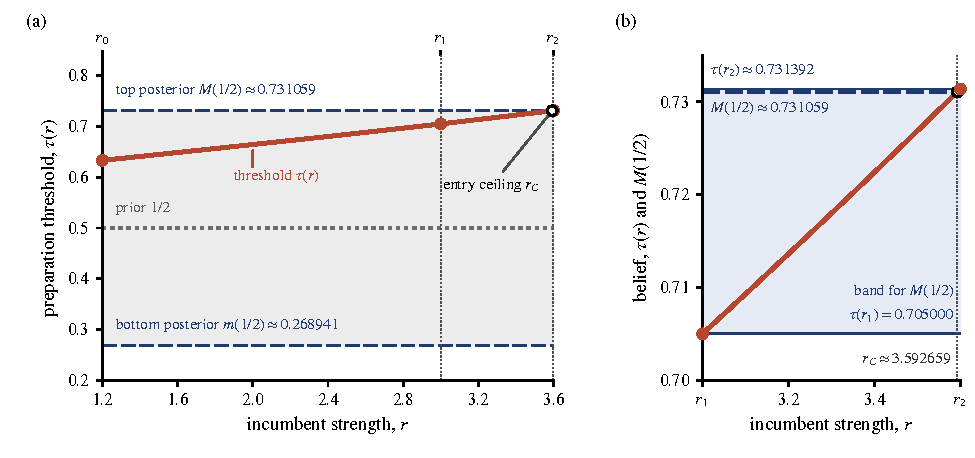
\includegraphics[width=\linewidth]{figures/beliefs.pdf}
\caption{Beliefs and the entry ceiling in the example.}\label{fig:beliefs}
\par\medskip
\begin{minipage}{\linewidth}\footnotesize\singlespacing
\textit{Notes.} Panel (a) plots the preparation threshold \(\tau(r)\) against incumbent strength \(r\). The gray band
covers the posteriors that an investor strategy can produce, from \(m(1/2)\) to \(M(1/2)\). The entry ceiling
\(r_C\) is the strength at which \(\tau(r)\) equals \(M(1/2)\). Panel (b) enlarges the strengths from \(r_1\) to
\(r_2\). Its blue band
holds every top posterior \(M(1/2)\) that puts \(r_C\) between \(r_1\) and \(r_2\); the example's value lies
\(\reg{margin_return_post_B}\) below the upper edge \(\tau(r_2)\).
\end{minipage}
\end{figure}

Figure~\ref{fig:beliefs} shows the preparation threshold along the path: the prior lies below it at every
strength, so an uninformative price never recruits a high-cost challenger, and the threshold rises with strength
until it meets the top posterior at the entry ceiling \(r_C\), just below \(r_2\). Panel~(b) shows the band of
Table~\ref{tab:region} for the top posterior (Corollary~\ref{cor:ccc-example-short}).

Holding the information in the price fixed while the incumbent strengthens removes the reversal. The experiment
fixes the law of the class and of a signal that the challenger observes, the class value laws and the cost law.
Given the class, the signal tells the challenger nothing more about either value. Its own value depends on
the signal only through the class; the incumbent's value is independent of the class and the signal, and the
two values are independent given the class and the signal. The cost is independent of the class, both values and the signal. A stronger incumbent then can only lower entry, for every such experiment and every independent cost law
(Proposition~\ref{prop:control} in Appendix~\ref{app:robustness} gives the formal condition): it lowers gross
profit at every belief, so it can only remove a preparation incentive, and entry falls by exactly the probability
that the cost lies between gross profit against the two incumbent distributions.

In the order slot the experiment fixes \(\lambda\), \(\beta\), \(\pi\), the cost law and both order distributions,
and competitive prices then reveal the same posterior after each order at every strength
(Appendix~\ref{app:beliefs}).

\begin{table}[tbp]
\centering\small\singlespacing
\caption{Equilibrium outcomes and information controls in the example.}\label{tab:outcomes}
\begin{tabular}{@{}lccc@{}}
\toprule
 & \(r_0=\reg{prim_r0}\) & \(r_1=\reg{prim_r1}\) & \(r_2=\reg{prim_r2}\)\\
\midrule
\multicolumn{4}{@{}l}{\emph{Panel A. Equilibrium (Proposition~\ref{prop:ccc})}}\\
Informed orders, classes \(H\) and \(L\) & \((0,0)\) & \((1,-1)\) & \((1,-1)\)\\
Posterior after a sale & \reg{p2_base_r0_mu_minus} & \reg{p2_base_r1_mu_minus} & \reg{p2_base_r2_mu_minus}\\
Posterior after no order & \reg{p2_base_r0_mu_zero} & \reg{p2_base_r1_mu_zero} & \reg{p2_base_r2_mu_zero}\\
Posterior after a purchase & \reg{p2_base_r0_mu_plus} & \reg{p2_base_r1_mu_plus} & \reg{p2_base_r2_mu_plus}\\
High-cost preparation & none & after a purchase & none\\
Price after a sale & \reg{price_r0} & \reg{price_r1_m1_B} & \reg{price_r2_m1_B}\\
Price after no order & \reg{price_r0} & \reg{price_r1_0_B} & \reg{price_r2_0_B}\\
Price after a purchase & \reg{price_r0} & \reg{price_r1_p1_B} & \reg{price_r2_p1_B}\\
Entry \(\Ent\) & \reg{entry_r0} & \reg{entry_r1_B} & \reg{entry_r2}\\
High-class ownership \(\Own_H\) & \reg{own_r0} & \reg{own_r1_B} & \reg{own_r2_B}\\
Expected target proceeds & \reg{p4_base_r0_proceeds} & \reg{p4_base_r1_proceeds} & \reg{p4_base_r2_proceeds}\\
\midrule
\multicolumn{4}{@{}l}{\emph{Panel B. Full orders held fixed (Proposition~\ref{prop:control})}}\\
Entry \(\Ent\) & \reg{p4_frozen_r0_entry} & \reg{p4_frozen_r1_entry} & \\
High-class ownership \(\Own_H\) & \reg{p4_frozen_r0_own} & \reg{p4_frozen_r1_own} & \\
Expected target proceeds & \reg{p4_frozen_r0_proceeds} & \reg{p4_frozen_r1_proceeds} & \\
\midrule
\multicolumn{4}{@{}l}{\emph{Panel C. The challenger does not see the price}}\\
Informed orders, classes \(H\) and \(L\) & \((0,0)\) & \((1,-1)\) & \\
Entry \(\Ent\) & \reg{p4_hidden_r0_entry} & \reg{p4_hidden_r1_entry} & \\
High-class ownership \(\Own_H\) & \reg{p4_hidden_r0_own} & \reg{p4_hidden_r1_own} & \\
Expected target proceeds & \reg{p4_hidden_r0_proceeds} & \reg{p4_hidden_r1_proceeds} & \\
\bottomrule
\end{tabular}
\par\medskip
\begin{minipage}{0.92\linewidth}\footnotesize
\textit{Notes.} The example. Panel A: the unique equilibrium at each strength. Panel B: full orders imposed at
both strengths; at \(r_0\) this profile is a control, not an equilibrium. Panel C: the unique equilibrium when the
challenger decides on its prior. At \(r_2\) the full-order profile is the equilibrium of Panel A.
\end{minipage}
\end{table}

Panel~B of Table~\ref{tab:outcomes} holds full orders fixed at both strengths. Only the top posterior can recruit
a high-cost challenger, because the preparation threshold \(\tau(r)\) exceeds the prior at every strength, so
entry is \(\reg{p4_frozen_r0_entry}\) at every strength up to the entry ceiling \(r_C\approx\reg{rC_B}\) and \(\rho\)
above it. Entry falls by the probability that the cost lies between gross profit at the two strengths, which
is \(\reg{p4_control_crossing_r0_r1}\) from \(r_0\) to \(r_1\) and \(\reg{p4_control_crossing_r1_r2}\) from
\(r_1\) to \(r_2\) (Proposition~\ref{prop:control}): with information fixed, entry stays
constant from \(r_0\) to \(r_1\) and falls above the entry ceiling.

Panel~C hides the price from the challenger, which then decides on its prior and prepares only at zero cost, so
entry stays at \(\reg{p4_hidden_r0_entry}\) at both strengths even though the investor trades fully at \(r_1\). The
two controls together locate the reversal in the information that trading generates: incumbent strength changes
that information, and the entry response to it exceeds the direct deterrence effect of a stronger incumbent at
fixed information.

\subsection{Coexistence}\label{sec:coexistence}

Between the weak and the strong incumbent of Proposition~\ref{prop:ccc}, two equilibria can hold against the same
incumbent. In a quiet market the investor does not trade, the price carries no information, and entry stays at its
floor; in the informative market that coexists with it, a purchase recruits a high-cost challenger. The two numbers
of Section~\ref{sec:twonumbers} decide where both exist: the threshold must lie above the prior and within reach of
a purchase, and the spread must be wide enough that a purchase that just reaches the threshold covers the trading
cost, yet narrow enough that no order against an uninformative price earns more than it.

\begin{proposition}[Quiet and informative markets]\label{prop:coexistence}
Let the classes satisfy the class ranking~\eqref{eq:classes}, let \(0<\pi<1\), \(0<\rho<1\), \(k>0\) and a slot
\((\lambda,\beta)\) be given, and let an indifferent investor mix over its best orders and an indifferent high-cost
challenger prepare. Take an incumbent distribution with a positive spread \(\DT\) and \(g_H>g_L\), and write \(\tau\)
for its preparation threshold.
\begin{enumerate}[label=(\alph*),leftmargin=2em]
\item A quiet market and an informative market coexist if and only if
\[
\pi<\tau\le M(\pi),\qquad \frac{k}{1-\tau}\le\DT\le\frac{k}{\rho\max\{\pi,1-\pi\}}.
\]
The informative market is then unique: class \(L\) abstains, only a purchase recruits a high-cost challenger, and
entry is
\[
\rho+(1-\rho)\min\Bigl\{\frac{(1-\pi)\,b\,\DT}{k},\;b+\pi\lambda\Bigr\},
\]
which rises strictly with the spread while class \(H\) mixes between a purchase and abstention and is constant once
class \(H\) buys for sure.
\item Along a path of such distributions, the strengths at which a quiet market coexists with an informative market
in which class \(H\) buys for sure form an interval, and every other strength with coexistence lies below it. Every
gap in coexistence lies at spreads too narrow for a sure purchase to pay.
\item Along a path on which the product of the spread and \(g_H-c_H\) does not fall with strength, the strengths
with coexistence form an interval, at every prior. Uniform incumbents on \([0,r]\), with \(r\) in a closed interval
above the reserve, satisfy this condition when every low-class value lies between the reserve and the lowest
strength, every high-class value is at least the highest strength, and class \(H\)'s mean value exceeds the highest
strength by at least \(c_H\).
\end{enumerate}
\end{proposition}

Coexistence comes from the entry response itself. In a quiet market entry stays at its floor after every order, so an
informed order earns at most \(\rho\max\{\pi,1-\pi\}\) times the spread, and the upper bound on the spread keeps that
from exceeding the trading cost. An informative market changes the entry response to a purchase, and with it the
return to trade: a purchase that reaches the threshold recruits, and the lower bound on the spread lets it cover the
trading cost.

Entry rises with the spread while class \(H\) mixes, because the purchase rate adjusts. While class \(H\) mixes, a
recruiting purchase earns exactly the trading cost, so a wider spread needs a more informative purchase; the purchase
rate rises, and entry rises with it until class \(H\) buys for sure. Entry depends on the incumbent only through the
spread, so between two incumbents at which the markets coexist, entry in the informative market is at least as high
against the one with the wider spread.

A stronger incumbent never narrows the spread, and where the threshold is positive it never lowers the threshold, so
the two numbers pull in opposite directions: a wider spread raises what a recruiting purchase earns, and a higher
threshold makes recruitment harder. As the incumbent strengthens, the economy can enter the region, leave it, and
enter it again. The strengths with a sure purchase are never split, because each condition that defines them holds on
one side of a single strength, and a mixed purchase needs a narrower spread than a sure one, so the other strengths
with coexistence lie below them. When class \(H\)'s gross profit exceeds the high cost against the weakest incumbent,
the whole set stays in one piece if the spread grows, in proportion, at least as fast as that excess shrinks;
part~(c) states the condition as a product, which does not fall.

The example satisfies the condition of Proposition~\ref{prop:coexistence}(c): its incumbent is uniform, \(\ell\) lies
between \(p\) and \(r_0\), and \(h\) exceeds \(r_2\) by more than \(c_H\), so at every prior the strengths with
coexistence form one interval. At the prior \(1/2\) the interval starts at \(r_A\), where a purchase that just
reaches the threshold and recruits earns the trading cost, and it ends at \(r_N\), where a unit order against an
uninformative price earns the trading cost. Class \(H\) buys for sure from \(r_F\), where a full purchase that
recruits earns the trading cost.

\begin{corollary}[Coexistence in the example]\label{cor:example-coexistence-short}
In the example at the prior \(1/2\), let the slot lie in the band of Corollary~\ref{cor:ccc-example-short}, and let an
indifferent investor mix over its best orders and an indifferent high-cost challenger prepare. An equilibrium exists
at every strength of the path from \(r_0\) to \(r_2\), and the strengths at which a quiet market and an informative
market coexist form the interval \([r_A,r_N]\). In the informative market that coexists with a quiet market, entry
is \(\rho+(1-\rho)\min\{b\DT(r)/(2k),\,b+\lambda/2\}\); it rises strictly on \([r_A,r_F]\) and is constant on
\([r_F,r_N]\). With a full purchase, entry keeps this value up to the entry ceiling \(r_C\) and equals \(\rho\) above
it.
\end{corollary}

\begin{figure}[tbp]
\centering
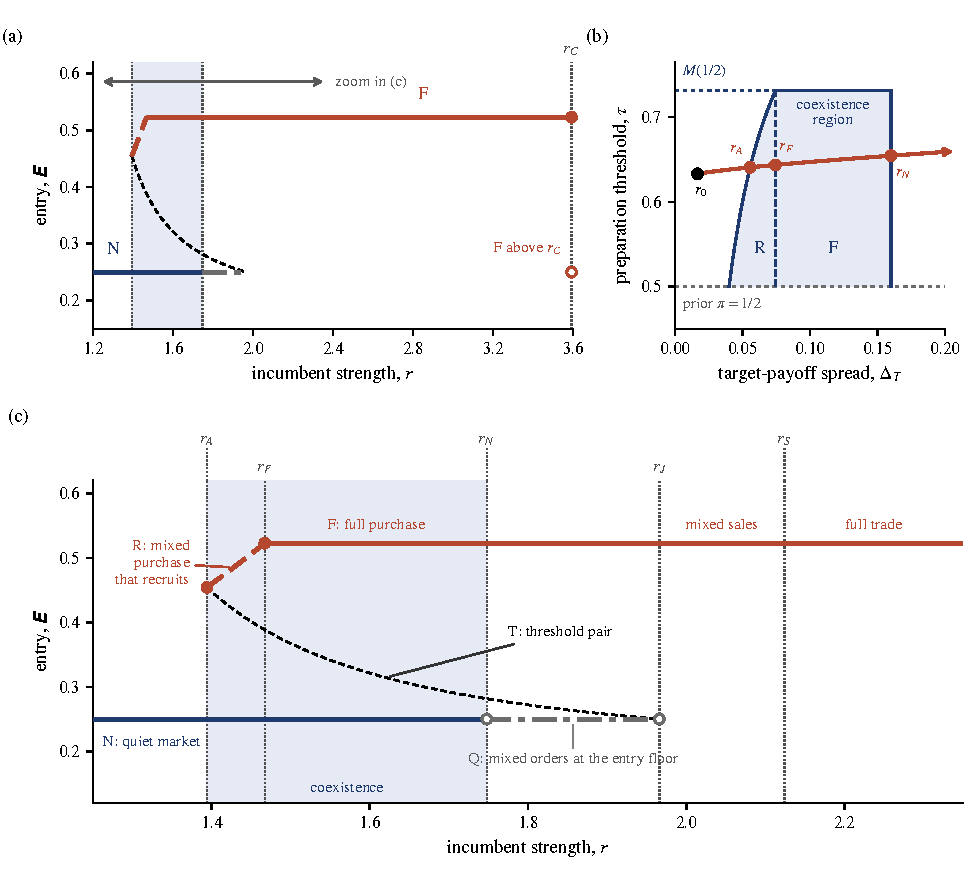
\includegraphics[width=\linewidth]{figures/coexistence.pdf}
\caption{Entry and the coexistence region along the example's path.}\label{fig:coexistence}
\par\medskip
\begin{minipage}{\linewidth}\footnotesize\singlespacing
\textit{Notes.} The example at the prior \(1/2\), when an indifferent investor may mix over its best orders and an
indifferent high-cost challenger prepares. Panels (a) and (c) show entry against incumbent strength \(r\) in each
equilibrium of Corollary~\ref{cor:example-coexistence}. Panel (a) covers the path from \(r_0\) to \(r_2\), and panel
(c) enlarges the strengths around the coexistence interval, which the blue band marks from \(r_A\) to \(r_N\). The
figure labels a quiet market by N, a mixed purchase that recruits by R, a full purchase by F, mixed orders at the
entry floor by Q and the threshold pair by T. The thin dashed line is the threshold pair~T. At \(r_A\) its purchase
recruits with probability one, and it is an equilibrium under the default tie rules; on \((r_A,r_J]\) it is an
equilibrium when an indifferent high-cost challenger may prepare with any probability. With a full purchase the low
class abstains up to \(r_N\), mixes from \(r_N\) to \(r_S\), and sells with probability one from \(r_S\); above the
entry ceiling \(r_C\), entry with a full purchase equals \(\rho\). Panel (b) draws the region of
Proposition~\ref{prop:coexistence}(a) at the example's slot, in the plane of the target-payoff spread \(\DT\) and
the preparation threshold \(\tau\): \(1/2<\tau\le M(1/2)\) and \(k/(1-\tau)\le\DT\le2k/\rho\). The dotted lower
edge, where \(\tau\) equals the prior, lies outside the region, and the other three edges belong to it. The dashed line
\(\DT=k/(1-M(1/2))\) divides the mixed purchase R, on its left, from the full purchase F. The curve traces
\((\DT(r),\tau(r))\) from \(r_0\): it enters the region at \(r_A\), reaches full purchases at \(r_F\), leaves the
region at \(r_N\), and continues towards \(r_1\) and \(r_2\) beyond the panel. Filled markers belong to a curve, and
open markers do not.
\end{minipage}
\end{figure}

In the example's slot, coexistence runs from \(r_A\approx\reg{rA}\) to \(r_N\approx\reg{rN}\), and class \(H\) buys
for sure from \(r_F\approx\reg{rF_B}\). Between \(r_A\) and \(r_F\) class \(H\) buys at the rate
\(b\,[\DT(r)/k-2]\), which rises with the spread until it reaches \(\lambda\) at \(r_F\), so entry in the informative
market is \(\reg{entry_rA_B}\) at \(r_A\), \(\reg{entry_mb_r140_B}\) at \(\reg{str_r140}\) and
\(\reg{entry_mb_r145_B}\) at \(\reg{str_r145}\); from \(r_F\) it stays at \(\reg{entry_r1_B}\) up to the entry
ceiling \(r_C\approx\reg{rC_B}\). Above \(r_N\) the informative market with a full purchase remains, and on
\((r_N,r_J)\), with \(r_J\approx\reg{rJ}\), mixed orders at the entry floor join it. The low class abstains up to
\(r_N\), mixes on \((r_N,r_S)\) and sells for sure from \(r_S\approx\reg{rS_B}\), the strength at which a full sale
earns the trading cost. Figure~\ref{fig:coexistence} draws the path through the region and the entry it produces,
and Appendix~\ref{app:coexistence} lists every equilibrium along the path.

The example's high cost lies between the two bounds that these conditions place on it. It is at most
\(h-r_2=\reg{cH_afford_ceiling_B}\), so class \(H\)'s value covers the high cost against the strongest incumbent
and Proposition~\ref{prop:coexistence}(c) applies, and it is at least \((h^2-p^2)/(2h)=\reg{cH_DA_floor_B}\), so
class \(H\) has the decisive advantage of Section~\ref{sec:ccc}.

Coexistence also holds away from the even prior. In the example's slot it starts at the same strength \(r_A\) for
every prior between \(\approx\reg{piA_lo_B}\) and \(\approx\reg{piA_hi}\), and it starts later, where the prior
reaches the threshold, for priors up to \(\approx\reg{pimax}\). Below \(\approx\reg{piA_lo_B}\) even the top
posterior cannot reach the threshold once a purchase can pay for itself, and from \(\approx\reg{pimax}\) on, the
quiet market ends before the prior falls below the threshold. Appendix~\ref{app:coexistence} gives the coexistence
set at every prior (Corollary~\ref{prop:priors}).

\section{Competition creates research}\label{sec:research}

So far the investor is present with a fixed probability \(\lambda\); now the investor chooses that probability and
pays for it. Before it learns the class, the investor chooses a research intensity \(\lambda\in[0,\lb]\) at the
cost \((a/2)\lambda^2\), where \(a>0\) and the cap satisfies \(0<\lb<1\). Research succeeds with probability
\(\lambda\), independently of the class, the costs and the incumbent's value. A success reveals the class, and the
investor then fills the slot with an order. After a failure, a liquidity trader fills the slot.

Research is therefore the presence probability of Section~\ref{sec:slot}, chosen at a cost. It is the specialist's
own work on the target's customers, technology and demand, and it must end before the order opportunity. The cap
\(\lb\) is the probability that this work can reveal the class at all before the challenger decides, because some
facts about the match become visible only through the buyer's own diligence. The marginal cost rises because the
specialist uses cheap sources first, such as its sector coverage, and costly ones later, such as expert calls. The
quadratic cost is the simplest form whose marginal cost rises.

A success takes the place of a liquidity order because the opportunity has room for one order. An investor that
knows the class takes it. After a failure, the investor knows no more than the market, so an order would lose at
least its cost \(k\). The opportunity then passes to a liquidity trader. More research therefore also removes
liquidity orders, and it reduces the camouflage of the investor's own orders.

Market makers and the challenger do not observe the research choice, so they price and decide at a conjectured
intensity; throughout this section the prior is \(1/2\). In an equilibrium with research, the conjectured
intensity is the investor's best research choice at the equilibrium prices and entry rule, and the order after
a success is optimal, including after a deviation from zero research.
The best research choice is unique: it equals the expected trading payoff after a success divided by \(a\), capped
at \(\lb\), so research never has a tie. Appendix~\ref{app:research} states the equilibrium with research
formally and gives each result of this section in full.

Research raises the top posterior that a purchase can reach. At intensity \(\lambda\), I write \(M_\lambda\) for
that top posterior and \(m_\lambda=1-M_\lambda\) for the bottom posterior, the posterior bounds of
Section~\ref{sec:inference} at the prior \(1/2\) when the presence probability is \(\lambda\). When
\(1/2<\tau(r)<1\), the \emph{recruitment intensity} \(\lambda_E(r)\) is the research level at which a full purchase
just reaches the threshold, \(M_\lambda=\tau(r)\), so a full purchase recruits exactly when research is at least
\(\lambda_E(r)\).

Suppose that class \(H\) buys after a success, class \(L\) abstains, and only a purchase recruits. A purchase
then earns \(\DT(r)m_\lambda-k\), and research optimality at an interior intensity reads:
\begin{equation}\label{eq:research}
2a\lambda=\DT(r)\,m_\lambda-k .
\end{equation}
The left side rises with \(\lambda\), and the right side falls, because more research removes camouflage. When
\(\DT(r)>2k\), the two sides meet at one intensity \(\lambda_R(r)\in(0,1)\).

On the branch where only a purchase recruits, a wider target-payoff spread raises the return to a purchase, so
the investor chooses more research and a purchase becomes more likely; research, entry and high-class ownership
then rise together with incumbent strength. At the benchmark strengths, the same force takes the economy from no
research and no trade against the weak incumbent, through coexistence of zero research with the research branch at
intermediate strengths, to research at the cap with trade in both directions against the strong and the very
strong incumbent. The benchmark research parameters are \(a=\reg{res_a}\) and the cap \(\lb=\reg{res_cap}\), the
presence probability of Section~\ref{sec:benchmark}, so research at the cap reproduces the benchmark slot.

\begin{proposition}[Competition creates research]\label{prop:research}
Let the auction be the benchmark auction at the prior \(1/2\), and suppose that \(0<\beta\le1/3\) and \(a>0\).
\begin{enumerate}[label=(\alph*),leftmargin=2em]
\item On the strengths with \(\DT(r)>2k\), research \(\lambda_R(r)\) is continuously differentiable and rises
strictly in \(r\). Wherever the research branch is an equilibrium, entry
\(\rho+(1-\rho)\bigl[\beta+(1/2-\beta)\lambda_R(r)\bigr]\) and high-class ownership
\(\tfrac12[\rho+(1-\rho)(\beta+(1-\beta)\lambda_R(r))]\) rise strictly with \(r\).
\item At the benchmark, with the research cost \(a=\reg{res_a}\) and the cap \(\lb=\reg{res_cap}\):
\begin{enumerate}[label=(\roman*),leftmargin=2em]
\item At \(r_0\), the unique equilibrium has no research and no trade. Entry is \(\rho\).
\item At each \(r\in\{\reg{str_r155},\reg{str_r160},\reg{str_r165}\}\), there are exactly two equilibria. In the
first, the investor does no research, and entry is \(\rho\). In the second, the research branch, research is
\(\lambda_R(r)\), with \(\lambda_E(r)<\lambda_R(r)<\lb\). After a success, class \(H\) buys and class \(L\) abstains,
only a purchase recruits, and entry is \(\rho+(1-\rho)[\beta+(1/2-\beta)\lambda_R(r)]\).
\item At \(r_1\) and \(r_2\), the unique equilibrium has research at the cap and trade in both directions. It is the
equilibrium of Proposition~\ref{prop:ccc} with \(\lambda=\lb\). Entry is \(\reg{res_entry_r1}\) at \(r_1\) and
\(\rho\) at \(r_2\).
\end{enumerate}
\end{enumerate}
\end{proposition}

At \(r_0\) every nonzero order after a success loses, so the expected trading payoff after a success is zero and
the best research choice is zero. At the intermediate strengths, the equilibrium without research confirms itself: against an
uninformative price the best nonzero order after a success earns \(\rho\DT/2-k<0\), because these strengths lie
below \(r_N\); on the research branch, a purchase reveals enough to recruit, and its return pays for the research
that makes it informative.

At \(r_1\) and \(r_2\), a bound on every candidate profile makes a full order profitable net of the marginal
research cost at the cap. Every trade
choice at the six strengths is strict, so the lists do not depend on how an indifferent investor breaks a tie.

\begin{table}[tbp]
\centering\small\singlespacing
\caption{Research and entry at the intermediate strengths.}\label{tab:research}
\begin{tabular}{@{}lccc@{}}
\toprule
 & \(r=\reg{str_r155}\) & \(r=\reg{str_r160}\) & \(r=\reg{str_r165}\)\\
\midrule
Target-payoff spread \(\DT(r)\) & \reg{res_Delta_r155} & \reg{res_Delta_r160} & \reg{res_Delta_r165}\\
Preparation threshold \(\tau(r)\) & \reg{res_tau_r155} & \reg{res_tau_r160} & \reg{res_tau_r165}\\
Recruitment intensity \(\lambda_E(r)\) & \reg{res_lamE_r155} & \reg{res_lamE_r160} & \reg{res_lamE_r165}\\
Research \(\lambda_R(r)\) & \reg{res_lambda_r155} & \reg{res_lambda_r160} & \reg{res_lambda_r165}\\
Posterior after a purchase \(M_{\lambda_R}\) & \reg{res_muplus_r155} & \reg{res_muplus_r160} & \reg{res_muplus_r165}\\
Entry on the research branch & \reg{res_entry_r155} & \reg{res_entry_r160} & \reg{res_entry_r165}\\
High-class ownership on the branch & \reg{res_own_r155} & \reg{res_own_r160} & \reg{res_own_r165}\\
Entry without research & \reg{entry_r0} & \reg{entry_r0} & \reg{entry_r0}\\
\bottomrule
\end{tabular}
\par\medskip
\begin{minipage}{0.92\linewidth}\footnotesize
\textit{Notes.} The benchmark with \(a=\reg{res_a}\) and \(\lb=\reg{res_cap}\). The spread, the threshold and
\(\lambda_E\) are exact rationals; research and the values that depend on it are interval enclosures rounded to six
places.
\end{minipage}
\end{table}

Research and entry rise together across the three intermediate strengths in Table~\ref{tab:research}: research
rises from \(\reg{res_lambda_r155}\) through \(\reg{res_lambda_r160}\) to \(\reg{res_lambda_r165}\), and entry rises
from \(\reg{res_entry_r155}\) through \(\reg{res_entry_r160}\) to \(\reg{res_entry_r165}\). A stronger incumbent
widens the target-payoff spread, so a purchase earns more and the investor chooses more research; the posterior
after a purchase then rises above the threshold by more, and a purchase becomes more likely. Part (a) of
Proposition~\ref{prop:research} shows that this comovement is general along the branch.

The slope of entry is \((1-\rho)(1/2-\beta)\lambda_R'(r)\), which is positive for every \(\beta\le1/3\). A purchase
has probability \(\beta+(1/2-\beta)\lambda\): research adds informed purchases in class \(H\) and removes liquidity
orders in both classes, and the first effect dominates.

At the benchmark, the research branch is an equilibrium exactly on \([r_R,\bar r_R)\), with
\(r_R\approx\reg{res_rR}\) and \(\bar r_R\approx\reg{res_rcap}\). The start \(r_R\) is the strength at which the purchase
posterior just reaches the threshold and the purchase also pays the marginal research cost:
\(\DT(1-\tau)=k+2a\lambda_E(r)\). The end \(\bar r_R\) is the strength at which research reaches the cap \(\lb\). Along
the branch, research rises from \(\lambda_E(r_R)=\reg{res_lambda_rR}\) to the cap, and entry rises from
\(\reg{res_entry_rR}\) to \(\reg{res_entry_cap}\). Zero research is an equilibrium along the whole branch, because
\(\bar r_R<r_N=\reg{res_rN}\). On \([\bar r_R,r_N)\), research at the cap coexists with zero research, and entry equals
\(\reg{res_entry_cap}\).

Against strong incumbents, research sits at the cap. Above a strength \(r_U\approx\reg{res_rUR}\),
a bound on every candidate profile forces full orders and research at the cap
(Appendix~\ref{app:research}).

\begin{figure}[tbp]
\centering
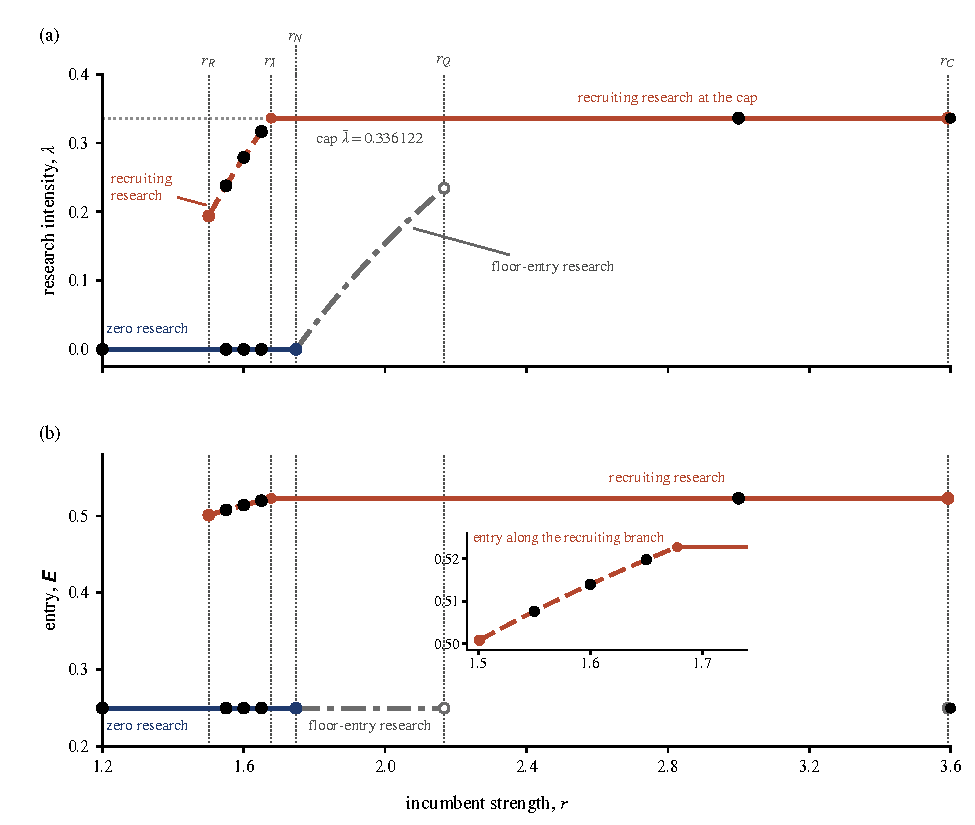
\includegraphics[width=\linewidth]{figures/research.pdf}
\caption{Research and entry along the research branch.}\label{fig:research}
\par\medskip
\begin{minipage}{\linewidth}\footnotesize\singlespacing
\textit{Notes.} The benchmark with \(a=\reg{res_a}\) and \(\lb=\reg{res_cap}\), where an indifferent high-cost
challenger prepares. Panel (a) shows research \(\lambda\), and panel (b) shows entry; the inset enlarges entry
along the research branch. Zero research is an equilibrium from \(r_0\) to \(r_N\). The research branch runs from
\(r_R\) to \(\bar r_R\). Research stays at the cap from \(\bar r_R\) to \(r_N\) and above \(r_U\); at the cap, entry
is \(\reg{res_entry_cap}\) up to the entry ceiling \(r_C\) and \(\rho\) above. Black dots mark the six strengths of
Proposition~\ref{prop:research}(b). The gray band marks the interval \((r_N,r_U)\) between the two cap ranges,
and the horizontal axis is broken there.
\end{minipage}
\end{figure}

The research branch in Figure~\ref{fig:research} starts later than the informative branch of
Section~\ref{sec:coexistence}, which starts at \(r_A=\reg{res_rA}\), because a purchase must now pay for research
as well as for trade. The two branches also adjust in different ways: with a fixed presence probability the
purchase rate adjusts through a mixture of the high class, while with research the intensity adjusts and the high
class buys with probability one after a success.

Proposition~\ref{prop:researchregion} in Appendix~\ref{app:research} gives the admissible
region of the research parameters exactly at \(\beta=\reg{beta_B}\). The equilibrium patterns of
Proposition~\ref{prop:research}(b) hold with strict margins exactly when the cap lies in the strip
\((\lambda_E(r_1),\lambda_E(r_2))\approx(\reg{res_cap_lo},\reg{res_cap_hi})\) and the cost lies in a window that
depends on the cap. At the benchmark cap, this window is \((\reg{res_a_lo},\reg{res_a_up})\). With \(1+u=\eu\), the
cap \(\lb=u\beta/(1+u\beta)\) and \(a=\reg{res_a}\), these patterns hold for every
\(\beta\in(\reg{res_beta_lo},1/3]\). Entry at \(r_1\) is \(\rho+(1-\rho)[\beta+(1/2-\beta)\lb]\).

\section{Robustness}\label{sec:robustness}

I vary one part of the model at a time: the preparation-cost law, the value classes and the prior, and the
challenger's information. Appendix~\ref{app:robustness} states each result in full and proves
it.

\subsection{Preparation costs}\label{sec:costs}

The rise of entry in Proposition~\ref{prop:ccc} survives other preparation-cost laws, with or without atoms
(Proposition~\ref{prop:atomless}). The cost now mixes a low component with weight \(\rho\) and a high
component in place of the two-point law of Section~\ref{sec:values}; either component may be atomless or have
atoms. The proposition keeps parts (i) and (ii) of Proposition~\ref{prop:ccc} under the trading-cost window (H2)
when every cost in the low component lies strictly below \(B_{F_1}(m(\pi))\) and every cost in the high component
lies strictly between \(B_{F_0}(\pi)\) and \(B_{F_1}(M(\pi))\). The low component then prepares at every feasible
belief, so entry stays at least \(\rho\), and the trading bounds of Section~\ref{sec:informed} apply unchanged.

At the benchmark, the low component runs from zero to \(\reg{atom_L}\), and the high component is uniform on
\([c_H-\varepsilon,c_H+\varepsilon]\). Every half-width below \(\reg{p4_atomless_max_width_floor_r2}\) keeps all
three parts of Proposition~\ref{prop:ccc}. With half-width \(\varepsilon=\reg{atom_eps}\),
entry at \(r_1\) is \(\reg{p4_atomless_r1_entry}\), the value under the two-point law. At \(r_2\), gross profit at
the top posterior, which lies \(\reg{margin_return_B}\) below \(c_H\), falls inside this band, and entry at \(r_2\)
is \(\reg{p4_atomless_r2_entry}\). With an atomless high component, the drop at the entry ceiling becomes a ramp:
full-order entry is continuous and nonincreasing in strength.

\subsection{Value classes and priors}\label{sec:classes}

The reversal holds for every pair of ranked classes and every prior. The classes satisfy the class
ranking~\eqref{eq:classes} and have different means, and the reserve, the prior, the zero-cost probability and the
slot are arbitrary. For uniform incumbents, a nonempty open set of strengths and costs then satisfies (H1)--(H3)
and the ownership condition of Proposition~\ref{prop:ccc} (Proposition~\ref{prop:classes}).

The construction puts the weak and the strong incumbent
just above the lowest value \(v_*\) at which the classes start to differ above the reserve. The spread vanishes near
\(v_*\), so informed trade against the weaker incumbent cannot cover its cost. The profit gap stays near the full class
gap there, so a high cost that only a favorable price justifies fits inside it. In the point-mass case
\(v_*=\ell\), so the reversal holds for every \(h>\ell\).

Table~\ref{tab:classes} in Appendix~\ref{app:robustness} reports six economies with their own costs and
strengths. With wide uniform classes, entry rises from \(\reg{p2_ex_c_r0_entry}\) to
\(\reg{p2_ex_c_r1_entry}\), and high-class ownership rises although the high class can lose to the strong
incumbent; point masses at the same means leave entry at \(\reg{p2_ex_d_r1_entry}\). A prepared challenger keeps
\((\theta-\max\{p,R\})_+\), a convex function of its value, so a mean-preserving spread within a class weakly
raises gross profit at every belief.

With more than two classes, the reversal holds under a separation condition (Proposition~\ref{prop:manyclasses}).
The price reveals only the posterior mean of class proceeds. Separation asks for a gap between the
proceeds of each high-group class and every feasible posterior mean, and the same gap for the low group. In the
strong equilibrium, class proportions within each group then stay at their prior proportions, so the price reveals
the whole posterior vector.

A four-class economy near the benchmark satisfies separation with distance \(\reg{p2_groups_gamma}\).
Without separation, one price can carry two posterior vectors: a strict three-class
equilibrium has two orders with different posterior vectors and one price.

\subsection{Complementary private signals}\label{sec:signals}

The challenger can gain from the price even when its own information is more accurate than the investor's. A buyer
may know its integration plans, while investors who follow the target know its customers or its product market.
Proposition~\ref{prop:signals} represents the two sources with conditionally independent binary
signals. The investor's signal has accuracy \(a_T\), and the challenger's signal has accuracy \(d\).

The zero-cost challenger still prepares after every price and signal, so the price still reveals the public
posterior, and the challenger combines that posterior with its own signal. Under strict conditions on the costs,
the weak incumbent has zero orders and entry \(\rho\); the strong incumbent has full orders and entry above
\(\rho\). The conditions allow \(d>a_T\).

The signal example uses its own parameter vector \(S(B)\). It keeps the slot, the values, the reserve and the
prior of the benchmark, and it sets \(\rho=\reg{sig_rho}\), \(c_H=\reg{sig_cH}\), \(k=\reg{sig_k}\),
\(r_0=\reg{sig_r0}\) and \(r_1=\reg{sig_r1}\). With investor accuracy \(a_T=\reg{sig_aT}\) and challenger accuracy
\(d=\reg{sig_d}\), entry rises from \(\reg{p4_s_signal_r0_entry}\) to \(\reg{p4_s_signal_r1_entry}\).
A favorable signal alone does not justify high-cost preparation against the weak incumbent;
a favorable signal and a favorable price together do so against the strong incumbent. Both sources are needed:
without the challenger's signal, entry is \(\reg{p4_s_no_y_r0_entry}\) at both strengths.

With the accuracies of the signal example \(S(B)\), the benchmark has a unique equilibrium at each strength when
an indifferent investor may mix over its best orders. At \(r_0\), the investor mixes between
trade and abstention after either signal, and it trades with probability \(\reg{p4_b_signal_r0_buy_rate}\). At
\(r_1\), it buys with probability one after a favorable signal, and after an unfavorable signal it sells with
probability \(\reg{p4_b_signal_r1_sell_rate}\). Entry falls from \(\reg{p4_b_signal_r0_entry}\) to
\(\reg{p4_b_signal_r1_entry}\). When an investor that is indifferent between abstention and a nonzero order must
abstain, neither strength has an equilibrium.

At the benchmark itself, the conditions hold with \((a_T,d)=(\reg{sig_comp_aT},\reg{sig_comp_d})\).
Entry then rises from \(\reg{p4_comp_b_r0_entry}\) to \(\reg{p4_comp_b_r1_entry}\), and
without the challenger's signal it is \(\reg{p4_comp_b_no_y_r1_entry}\) at both strengths. A buyer signal at least
as accurate as the investor's needs other costs and strengths, as in the signal example: at the benchmark the
strong trading bound needs an accurate investor signal, and the weak bound then fails.

\section{Welfare and sale terms}\label{sec:welfare}

\subsection{Access to prices}\label{sec:access}

Access to prices improves acquisition outcomes at a fixed level of competition. At the strong incumbent
\(F_1\), I compare the equilibrium of Proposition~\ref{prop:ccc} with that of an economy in which the
rival does not see the price. Under the hypotheses of Proposition~\ref{prop:ccc}, both economies have unique full orders, and price access
raises expected target proceeds and acquisition surplus net of preparation costs
(Proposition~\ref{prop:access}).
Acquisition surplus excludes transfers between bidders, shareholders and traders, and
Appendix~\ref{app:welfare} states each result on welfare and sale terms in full.

The two economies generate the same orders. The trading bound of Section~\ref{sec:informed} forces full orders even
when the rival cannot use the price and entry stays at \(\rho\), so trading costs coincide. Price access
changes only which high-cost rivals prepare: it adds preparation after a purchase. Each added preparation
adds its gross profit minus its cost to net surplus, together with the value of any sale that the reserve
would otherwise block; a rival prepares only when its expected gross profit covers its cost, so no
added preparation lowers net surplus.

In the example at \(r_1\), expected proceeds rise from \(\reg{p2_base_hidden_proceeds}\) to
\(\reg{p2_base_r1_proceeds}\), a gain of \(\reg{p2_access_proceeds_gain}\), and net surplus rises by
\(\reg{p2_access_surplus_gain}\). With research at the cap (Section~\ref{sec:research}), the
gains are the same.

Target shareholders gain because a shareholder who holds through the sale receives \(V_T\), not the interim price.
The informed trader's expected gross profit, \(\reg{p2_access_gross_transfer}\) at \(r_1\), is a transfer from
liquidity traders. If one order unit is a given number of shares per share of float, initial shareholders gain in
total relative to an economy without the informed trader whenever that number is below \(\reg{p2_access_break_even}\), even if
they bear the whole transfer.

Inside the recruitment region of Proposition~\ref{prop:ccc}, where high-cost preparation does not pay at the prior,
price access adds preparation. When gross profit at the prior exceeds \(c_H\) and gross profit after a sale falls below it, an informative price
deters high-cost preparation after a sale: in the example at \(r_1\) with \(c_H=\reg{access_out_cH}\), price access changes proceeds by
\(\reg{p2_outside_proceeds_gain}\) and net surplus by \(\reg{p2_outside_surplus_gain}\)
(Appendix~\ref{app:welfare}).

The two economies differ in the information in the price and not in its level. A deterministic external dividend of
\(\reg{p2_access_proceeds_gain}\) in the hidden-price economy equalizes the mean prices, and it leaves the orders
and entry unchanged.

\subsection{The payment rule}\label{sec:payment}

The effect of competition on the target-payoff spread depends on the sale payment.
Proposition~\ref{prop:payment} isolates this dependence at the payment stage, in a
verifiable-value institution with zero reserve, point-mass classes and an incumbent distribution on \([0,\bar r]\)
with \(0<\ell<\bar r<h\). After diligence, a sale to the next bidder at its value is an
enforceable fallback, and the seller and the winner divide the surplus above the fallback by Nash bargaining, with
seller weight \(\omega\in[0,1)\). A stronger incumbent never raises the rival's profit, and it moves the
spread only in the direction of the sign of \(1-2\omega\); the move is strict when \(\E[(R-\ell)_+]\) changes
strictly and \(1-2\omega\ne0\), and when \(1-2\omega=0\) the spread equals \((h-\ell)/2\) at every incumbent
distribution.

To see why, take \(R>\ell\). A high-class rival wins and pays \((1-\omega)R+\omega h\), whose sensitivity to
\(R\) is \(1-\omega\). A low-class rival loses, and the incumbent pays \((1-\omega)\ell+\omega R\), whose
sensitivity is \(\omega\). Competition widens the difference exactly when the first sensitivity exceeds the second.

In the example, the spread under this rule changes by \(\reg{pay_gap_coef}\,(1-2\omega)\) from \(r_0\) to \(r_1\).
The second-price auction is the case \(\omega=0\): it puts the whole weight on the runner-up's value.
\citet{BulowKlemperer1996} compare an auction with one more bidder and an optimal negotiation by expected revenue;
here the comparison concerns how competition moves the spread.

\subsection{Reserves}\label{sec:reserves}

A reserve affects both the payment required to win and the information in the target's shares. Once the reserve can
exclude bidders, preparation, a sale and the meeting of two admissible bidders become different events:
\emph{preparation} is the event that the rival pays its preparation cost, a \emph{sale} occurs when at
least one bidder submits an admissible bid, and \emph{two admissible bidders} meet when both the incumbent
and a prepared rival meet the reserve. In the example of Section~\ref{sec:benchmark},
the reserve lies below both class values of the rival, so every prepared rival is admissible.

A reserve that excludes the low class can widen the class difference in target proceeds, because the low class then
adds nothing to proceeds. Informed trade can then pay against both incumbents, and the price is informative at both
strengths. Proposition~\ref{prop:reserves} gives the consequence. If informed trade is full at both strengths and only a purchase recruits at each,
entry is flat in incumbent strength, and strict deterrence needs the stronger incumbent to push gross profit at the
top posterior below the high cost.

\begin{table}[tbp]
\centering\small\singlespacing
\caption{Reserves, preparation and sale in the example.}\label{tab:reserves}
\begin{tabular}{@{}llcccc@{}}
\toprule
Reserve & Strength & Entry & Sale & Two admissible bidders & Expected proceeds\\
\midrule
\(\reg{prim_p}\) & \(r_0\) & \reg{p2_reserve_points_base_r0_entry} & \reg{p2_reserve_points_base_r0_sale} & \reg{p2_reserve_points_base_r0_two} & \reg{p2_reserve_points_base_r0_proceeds}\\
 & \(r_1\) & \reg{p2_reserve_points_base_r1_entry} & \reg{p2_reserve_points_base_r1_sale} & \reg{p2_reserve_points_base_r1_two} & \reg{p2_reserve_points_base_r1_proceeds}\\
\(\reg{rsv_points_excl}\) & \(r_0\) & \reg{p2_reserve_points_exclude_r0_entry} & \reg{p2_reserve_points_exclude_r0_sale} & \reg{p2_reserve_points_exclude_r0_two} & \reg{p2_reserve_points_exclude_r0_proceeds}\\
 & \(r_1\) & \reg{p2_reserve_points_exclude_r1_entry} & \reg{p2_reserve_points_exclude_r1_sale} & \reg{p2_reserve_points_exclude_r1_two} & \reg{p2_reserve_points_exclude_r1_proceeds}\\
\(\reg{rsv_deter}\) & \(r_0\) & \reg{p2_reserve_points_deter_r0_entry} & \reg{p2_reserve_points_deter_r0_sale} & \reg{p2_reserve_points_deter_r0_two} & \reg{p2_reserve_points_deter_r0_proceeds}\\
 & \(r_1\) & \reg{p2_reserve_points_deter_r1_entry} & \reg{p2_reserve_points_deter_r1_sale} & \reg{p2_reserve_points_deter_r1_two} & \reg{p2_reserve_points_deter_r1_proceeds}\\
\bottomrule
\end{tabular}
\par\medskip
\begin{minipage}{0.92\linewidth}\footnotesize
\textit{Notes.} The example, with point-mass classes. At each reserve, full informed orders are the unique outcome
at both strengths, except at the reserve \(\reg{prim_p}\) and \(r_0\), where the informed trader does not trade.
\end{minipage}
\end{table}

Table~\ref{tab:reserves} reports three reserves in the example. The reserve
\(\reg{rsv_points_excl}\) excludes the low class. Full orders are unique at both strengths, only a purchase recruits,
and entry is \(\reg{p2_reserve_points_exclude_r0_entry}\) at both \(r_0\) and \(r_1\), while this reserve raises
expected proceeds at both strengths. Narrow uniform classes give the same pattern at the reserve
\(\reg{rsv_bands_excl}\).

The reserve \(\reg{rsv_deter}\) restores strict deterrence: entry is \(\reg{p2_reserve_points_deter_r0_entry}\) at
\(r_0\) and \(\reg{p2_reserve_points_deter_r1_entry}\) at \(r_1\), and proceeds exceed their levels at the reserve
\(\reg{prim_p}\). This reserve excludes the low class and also the weak incumbent, since it exceeds \(r_0\). In the
example, strict deterrence with a reserve that excludes the low class requires the reserve to exclude the weak
incumbent as well. With a reserve in
\((\ell,r_0]\), the top posterior recruits at both strengths, and entry is flat. Strict deterrence holds for reserves
between about \(\reg{p2_reserve_ph}\) and \(\reg{p2_reserve_weak_top}\)
(Appendix~\ref{app:welfare}).

\section{Empirical implications}\label{sec:empirical}

The model gives predictions for publicly visible sale processes in which one bidder is prepared and a challenger has
not yet committed to diligence. Each prediction names the incumbent, prior, trading-pattern and tie-rule conditions
it needs, and concerns one target in one public state; Appendix~\ref{app:empirical} states each in full and proves
it. The predictions concern price impacts, the informed investor's presence, the winner and announcement returns.
Under full two-sided trade, class \(H\) buys and class \(L\) sells, each with probability one, and the informed share
of nonzero orders is \(u/(2+u)\) at every prior. In the example at the prior \(1/2\) and the example's slot, full
two-sided trade is the unique outcome at every strength between \(r_S\), the strength at which a full sale earns the
trading cost, and \(h\); this range contains \(r_1\), the entry ceiling \(r_C\) and \(r_2\).

\paragraph{Entry and incumbent strength.} When the price reaches the challenger before its decision, a stronger
prepared bidder can raise the probability that the challenger prepares; in the example, that probability rises by
\(\reg{entry_jump_B}\) from \(r_0\) to \(r_1\). When the price does not reach the challenger, a stronger prepared
bidder can only lower it. Against a strong enough prepared bidder, entry can return to its floor while the price stays
informative. Proposition~\ref{prop:ccc} gives the first and third comparisons, and the fixed-information control of
Section~\ref{sec:benchmark} gives the second (Proposition~\ref{prop:control}).

\paragraph{The price gap and its entry component.} Under full two-sided trade at a prior below the preparation
threshold, the purchase impact \(P(1)-P(0)\), weighted by the frequency of a purchase, exceeds the sale impact
\(P(0)-P(-1)\), weighted by the frequency of a sale, exactly when a purchase recruits the challenger
(Proposition~\ref{prop:spread}). The weighted difference equals the expected price before the order opportunity
minus the price after no order, so the test needs prices and order frequencies and no auction object; at the prior
\(1/2\) the two frequencies are equal, and the test compares the two impacts directly. Under the same conditions the
price gap \(P(1)-P(-1)\) has a class component, \(\rho\DT\,[M(\pi)-m(\pi)]\), and an entry component, which is
positive exactly when a purchase recruits; the whole entry component sits in the purchase impact. As the incumbent
strengthens, entry adds more to the price through competition and less by rescuing a sale that the incumbent alone
would not complete. With a uniform incumbent and the prior and the slot fixed, the entry component rises with
strength while full two-sided trade and recruitment persist, when \(3p^2<\min\{\underline\theta,\underline r\}^2\),
where \(\underline\theta\) is the lowest challenger value and \(\underline r\) the lowest strength compared; the
example meets this condition.

In the example at \(r_1\), the price gap is \(\reg{ba_r1_B}\), and its entry component is \(\reg{ba_share_r1_B}\) of
it. With a hidden price, the price gap would be \(\reg{ba_class_r1_B}\). At \(r_2\) the price gap is
\(\reg{ba_r2_B}\), the class component alone, and at the entry ceiling \(r_C\) it falls by \(\reg{ba_jump_rC_B}\).

\paragraph{The informed share.} Under full two-sided trade the mean order is \(\lambda(2\pi-1)\), so order counts
identify the informed investor's presence when the prior is known and differs from one half
(Proposition~\ref{prop:informedshare}). The sale impact identifies presence at any known prior, one half included:
when entry after a sale and after no order sits at its floor and the payoff scale \(\rho\DT\) is known, the sale
impact weighted by the frequency of a sale, divided by \(\rho\DT\), equals \(\pi(1-\pi)\lambda\), and together with
the mean order \(\lambda(2\pi-1)\) it identifies both the presence probability and the prior. At the prior
\(1/2\) the counts depend on the slot only through the volume of nonzero orders, so prices separate slots that counts
cannot. In the example at \(r_1\), the shares consistent with the counts and the investor's incentives form the
interval from \(\approx\reg{theta_min_counts_B}\) to \(\reg{theta_max_full_eq_r1_B}\), and a slot with share
\(\reg{alt_theta_B}\) has the example's volume and entry, but its price gap at \(r_1\) is \(\reg{alt_ba_r1_B}\),
against \(\reg{ba_r1_B}\).

\paragraph{Winners.} Under full two-sided trade, a prepared challenger wins more often after a purchase than after a
sale exactly when the incumbent's value falls, with positive probability, where a high-class value beats it with a
higher probability than a low-class value; the gap is \(M(\pi)-m(\pi)\) times the difference between the classes' chances of
beating the incumbent (Proposition~\ref{prop:winner}). Orders predict the winner even where they do not predict
entry: where entry stays at its floor after every order, as above the entry ceiling, the order still covaries
positively with a challenger win under the same condition, and not with entry. With the prior and the slot fixed and
full two-sided trade at each strength compared, when class \(H\) outbids every incumbent the gap does not narrow as
the incumbent strengthens, and it widens wherever the stronger incumbent takes wins from the low class. Among
prepared challengers, the share of the high class at each price is the price-implied posterior, which rises with the
price under full two-sided trade. In the example class \(H\) outbids every incumbent, and the gap is
\(\reg{wgap_r1_B}\) at \(r_1\) and \(\reg{wgap_r2_B}\) at \(r_2\); the covariance of the order with entry is
\(\reg{cov_entry_r1_B}\) at \(r_1\) and zero at \(r_2\).

\paragraph{Announcements.} For a positive target-payoff spread and \(g_H>g_L\), if a public event after the price reveals only whether the
challenger prepared, the mean price change over preparation reports is positive exactly when preparation was still uncertain after some order, at
every prior and in every equilibrium (Proposition~\ref{prop:announcement}); in the example it is
\(\reg{evprep_mean_r1_B}\) at \(r_1\). The mean change over both reports, with their model probabilities, is zero. Under
full two-sided trade at a prior below the preparation threshold, an opportunity that passes with no order is no news
about the class and, when a purchase recruits, bad news about entry: in the example at \(r_1\), the price after no
order minus the expected price before the opportunity is \(\reg{pdrop_neutral_r1_B}\), and the size of this drop is
the weighted difference of the price-impact test.

\paragraph{Two clusters at intermediate strengths.} In the example, at one public strength in the range
\((r_F,r_N)\) of Section~\ref{sec:coexistence}, processes can form two clusters. In one cluster the market is quiet:
the mean order is zero and the three prices coincide. In the other, the high class buys and the low class abstains;
the mean order is then \(\lambda/2\) (\(\reg{imb_buy_B}\) in the example), every challenger prepares after a purchase,
and a sale executes above the price after no order, by \(\reg{U_gap_r160_B}\) at \(\reg{str_r160}\).

\paragraph{Measurement.} The counterpart of preparation is the start of substantive diligence or a proposal that
requires costly preparation; public offers are a narrower outcome. Incumbent strength is measured from information
that is public before that decision, and the price must precede it.

The order is the first prespecified public order opportunity after the sale becomes public, and an opportunity with
no order is recorded as a zero. A scheduled call auction is one example, such as the opening auction on the first
trading day after the approach is disclosed; its time is fixed in advance and does not depend on any trader's
information, and the auction takes place whether or not an order arrives. The sign of its net order imbalance is the
order, and an imbalance below a size fixed in advance records the zero order. A sample of first executed trades omits
the zero order, so it cannot identify the volume, the effect of an inactive opportunity, or the informed share.

The announcement formulas need events that reveal only preparation. Target returns before a bid also
partly reflect anticipation of that bid \citep{Schwert1996}, so each test dates the price before the challenger's
decision. The trading counterpart is outside trade with a view on the challenger's fit, such as orders from sector
specialists.

\section{Conclusion}\label{sec:conclusion}

In the model, the bidder pool in a takeover depends on the information that buyers have before they commit to
preparation. A
stronger incumbent moves the class value gap from the challenger's profit to target proceeds, and because a
liquidity order can match the investor's direction in the order slot, an investor who knows the challenger's
class keeps a residual advantage after every order. A larger target-payoff spread can make that advantage worth
the cost of trade, so the price can recruit a challenger that a weaker incumbent fails to attract.

The comparison of the weak, strong and very strong incumbent holds with unique outcomes on an open set of
parameters (Proposition~\ref{prop:ccc}). Under the default tie rules, a quiet market and an informative market
coexist exactly on a region of the target-payoff spread and the preparation threshold
(Proposition~\ref{prop:coexistence}), and a stronger incumbent can move the economy into and out of that region; in
the informative market, entry rises with the spread while the high class mixes between a purchase and abstention
and stays constant once it buys for sure. When information is costly, competition creates research: at an even
prior, when an indifferent investor may mix over its best orders and the preparation threshold lies above the prior,
research and entry rise together with the spread until research reaches its cap, in the equilibrium in which a
purchase after successful research recruits (Proposition~\ref{prop:research}), and the low class's selling does not
interrupt the rise.

Sale terms affect entry through the challenger's expected payment and through the information in the stock price.
Under the hypotheses of the main result, access to prices raises target proceeds and acquisition surplus net of
preparation costs against the strong incumbent, and, with a single value in each class and the incumbent's highest
value between them, in a bargaining family of payment rules with a zero reserve, the weight that the rule places
on the runner-up's value decides the direction in which competition moves the target-payoff spread. A reserve that
excludes the low class can make the price informative against both
incumbents; if informed trade is then full and only a purchase recruits at both strengths, entry is flat in
incumbent strength.

The next theoretical step is the seller's choice of terms with the whole pricing and trading continuation retained.
The empirical tests ask whether the challenger's preparation in visible sale processes responds to incumbent
strength when the price precedes the decision, and, where the investor always buys after good news and always sells
after bad news and the prior lies below the preparation threshold, whether a purchase raises the price by more than a sale lowers
it once each impact is weighted by how often its order occurs, as Section~\ref{sec:empirical} predicts where a
purchase recruits.


\clearpage
\singlespacing
\bibliographystyle{aer}
\bibliography{references}

\clearpage
\onehalfspacing
\appendix
\renewcommand{\theequation}{A.\arabic{equation}}
\renewcommand{\theHequation}{A.\arabic{equation}}
\setcounter{equation}{0}
\renewcommand{\theproposition}{A.\arabic{proposition}}
\renewcommand{\theHproposition}{A.\arabic{proposition}}
\setcounter{proposition}{0}
\renewcommand{\thelemma}{A.\arabic{lemma}}
\renewcommand{\theHlemma}{A.\arabic{lemma}}
\setcounter{lemma}{0}
\renewcommand{\thecorollary}{A.\arabic{corollary}}
\renewcommand{\theHcorollary}{A.\arabic{corollary}}
\setcounter{corollary}{0}
\renewcommand{\thedefinition}{A.\arabic{definition}}
\renewcommand{\theHdefinition}{A.\arabic{definition}}
\setcounter{definition}{0}
\renewcommand{\theremark}{A.\arabic{remark}}
\renewcommand{\theHremark}{A.\arabic{remark}}
\setcounter{remark}{0}
\renewcommand{\thetable}{A.\arabic{table}}
\renewcommand{\theHtable}{A.\arabic{table}}
\setcounter{table}{0}
\renewcommand{\thefigure}{A.\arabic{figure}}
\renewcommand{\theHfigure}{A.\arabic{figure}}
\setcounter{figure}{0}
\section{Proofs}\label{app:proofs}

This appendix proves every result in the paper. Statements use the class model of Section~\ref{sec:model}. A
statement that needs the example says so. Each equilibrium proof states the equilibrium tuple of
Definition~\ref{def:equilibrium}, lists its conditions, and shows that the fixed tuple satisfies each of them.

% STRUCTURE: Definition 1 and the conditions (E1)-(E6) <- Section 2.4; eta <- Section 2.3
\paragraph{The equilibrium tuple.}
Write \(\eta(-1)=\eta(1)=\beta\) and \(\eta(0)=1-2\beta\) for the liquidity order distribution of
Section~\ref{sec:slot}.

\begin{definition}[Equilibrium]\label{def:equilibrium}
An \emph{equilibrium} is a tuple
\[
\mathcal{E}=\bigl(\sigma_H,\sigma_L,\ \mu,\ P,\ \bar\mu,\ \zeta\bigr),
\]
together with the bids of the prepared bidders. Its components are as follows.
\begin{itemize}[leftmargin=2em]
\item \(\sigma_j=\bigl(\sigma_j(-1),\sigma_j(0),\sigma_j(1)\bigr)\) is a probability distribution on
\(\{-1,0,1\}\), the order of the informed trader in class \(j\in\{H,L\}\). Mixed and wrong-signed orders are
allowed.
\item \(\mu:\{-1,0,1\}\to[0,1]\) is the market makers' posterior \(\mu(x)=\Pr(j=H\mid X=x)\).
\item \(P:\{-1,0,1\}\to\mathbb{R}\) is the price after each order.
\item \(\bar\mu\) assigns to each price \(\bar P\) in the image of \(P\) the rival's belief
\(\Pr(j=H\mid P(X)=\bar P)\).
\item \(\zeta(\bar P)\in[0,1]\) is the probability that a rival with the high cost prepares after the price
\(\bar P\). A rival with the zero cost prepares after every price.
\end{itemize}
For each order \(x\), write \(f_j(x)=(1-\lambda)\eta(x)+\lambda\sigma_j(x)\) for its probability in class
\(j\), and \(e(x)=\rho+(1-\rho)\,\zeta(P(x))\) for entry after it. The tuple satisfies six conditions.
\begin{enumerate}[label=(E\arabic*),leftmargin=3em]
\item \emph{Bayes consistency.} For every order \(x\),
\(\mu(x)=\pi f_H(x)/[\pi f_H(x)+(1-\pi)f_L(x)]\).
\item \emph{Beliefs of the rival.} For every price \(\bar P\) in the image of \(P\), \(\bar\mu(\bar P)\) is the
posterior of class \(H\) given the event \(\{x:P(x)=\bar P\}\), computed from \(f_H\) and \(f_L\).
\item \emph{Entry optimality.} For every price \(\bar P\) in the image, \(\zeta(\bar P)=1\) if
\(B(\bar\mu(\bar P))>c_H\) and \(\zeta(\bar P)=0\) if \(B(\bar\mu(\bar P))<c_H\). At
\(B(\bar\mu(\bar P))=c_H\), the rival's tie rule applies.
\item \emph{Competitive prices.} For every order \(x\), \(P(x)=\E[V_T\mid X=x]\).
\item \emph{Optimality of the informed trader.} For each class \(j\), \(\sigma_j(q)>0\) only if \(q\) maximizes
\[
U_j(q)=q\,\bigl[t_0+e(q)(t_j-t_0)-P(q)\bigr]-k|q|
\]
over \(q\in\{-1,0,1\}\), with \(P(\cdot)\) and \(e(\cdot)\) held at their values in \(\mathcal{E}\).
\item \emph{Truthful bids.} Each prepared bidder whose value meets the reserve bids its value.
\end{enumerate}
\end{definition}

The gross profit of a zero-cost rival is an expected auction rent, which is never negative. Preparation is
therefore optimal for it after every price, and the definition fixes this choice. The probability \(f_j(x)\) is
at least \((1-\lambda)\eta(x)>0\) under every strategy. Every order therefore occurs with positive probability in
both classes. Bayes' rule defines \(\mu\) after every order, and no off-path belief enters the definition.

The two indifferences in (E3) and (E5) follow the default tie rules of Section~\ref{sec:equilibrium}: an
indifferent informed trader may mix over its best orders, and an indifferent high-cost rival prepares.
Appendix~\ref{app:coexistence} states the alternatives, under which an indifferent informed trader abstains or an indifferent
high-cost rival may prepare with any probability.

\subsection{Acquisition payoffs}\label{app:payoffs}

\paragraph{Truthful bids.}
Fix a bidder with value \(\theta\), and let \(Y\ge0\) be the highest competing admissible bid, with \(Y=0\) when
there is none. Any admissible bid that wins pays \(\max\{p,Y\}\), so a bid yields either \(\theta-\max\{p,Y\}\) or
zero. Suppose \(\theta\ge p\), and consider the bid \(\theta\). If \(\theta>\max\{p,Y\}\), it wins and earns
\(\theta-\max\{p,Y\}>0\). If \(\theta<\max\{p,Y\}\), then \(Y>\theta\), and the bid loses and earns zero. If
\(\theta=\max\{p,Y\}\), a win pays \(\theta\), so the bid earns zero.

The bid \(\theta\) therefore earns \((\theta-\max\{p,Y\})_+\), the larger of the two possible payoffs, at every \(Y\).
Suppose \(\theta<p\). Every bid that wins pays at least \(p>\theta\), so no bid earns more than zero, the payoff of no
bid. Truthful bids, and no bid below the reserve, are therefore weakly dominant at every competing bid. Hence
condition (E6) of Definition~\ref{def:equilibrium} holds in every tuple. No payoff below rests on a belief.

\paragraph{Proof of Proposition~\ref{prop:returns}.}
Without entry the target receives \(p\1\{R\ge p\}\). A prepared rival with \(\theta\ge p\) wins at
\(\theta>R\) and pays \(\max\{p,R\}\). A loss makes the incumbent pay \(\theta\). The target receives
\(\max\{p,\min(R,\theta)\}\), and the rival keeps \((\theta-\max\{p,R\})_+\). At \(\theta<p\) the
rival does not bid. The target again receives \(p\1\{R\ge p\}\), and the rival keeps nothing.

\emph{The example.} Let \(R\) be uniform on \([0,r]\) with \(0<p<\ell<r<h\), as in \eqref{eq:order}. Then
\(t_0=\Pr(R\ge p)\,p=p(1-p/r)\). Since \(R\le r<h\), the high-class rival always wins and pays
\(\max\{p,R\}\). The low-class rival wins and pays \(\max\{p,R\}\) when \(R<\ell\); it loses when
\(R\ge\ell\). Integration over \(R\) gives
\begin{equation}\label{eq:a-payoffs}
\begin{aligned}
t_H&=\frac1r\Bigl[\int_0^p p\,dy+\int_p^r y\,dy\Bigr]
=\frac1r\Bigl[p^2+\frac{r^2-p^2}2\Bigr]=\frac r2+\frac{p^2}{2r},\\
t_L&=\frac1r\Bigl[\int_0^p p\,dy+\int_p^\ell y\,dy+\int_\ell^r\ell\,dy\Bigr]
=\frac1r\Bigl[p^2+\frac{\ell^2-p^2}2+\ell(r-\ell)\Bigr]=\ell-\frac{\ell^2-p^2}{2r},\\
g_H&=\frac1r\int_0^r\bigl(h-\max\{p,y\}\bigr)\,dy=h-t_H=h-\frac r2-\frac{p^2}{2r},\\
g_L&=\frac1r\Bigl[\int_0^p(\ell-p)\,dy+\int_p^\ell(\ell-y)\,dy\Bigr]
=\frac1r\Bigl[p(\ell-p)+\frac{(\ell-p)^2}2\Bigr]=\frac{\ell^2-p^2}{2r}.
\end{aligned}
\end{equation}

The spread is
\[
\DT(r)=t_H-t_L=\frac r2+\frac{p^2}{2r}-\ell+\frac{\ell^2-p^2}{2r}=\frac{r^2-2\ell r+\ell^2}{2r}
=\frac{(r-\ell)^2}{2r}.
\]
The sums are \(t_H+g_H=h\) and \(t_L+g_L=\ell\), as the split requires. These are the expressions in \eqref{eq:payoffs}.

Differentiation in \(r\) gives
\[
\begin{gathered}
\DT'(r)=\frac{2(r-\ell)\cdot2r-2(r-\ell)^2}{4r^2}=\frac{(r-\ell)(r+\ell)}{2r^2}=\frac12-\frac{\ell^2}{2r^2},\\
g_H'(r)=-\frac12+\frac{p^2}{2r^2},\qquad g_L'(r)=-\frac{\ell^2-p^2}{2r^2}.
\end{gathered}
\]
The signs in \eqref{eq:derivatives} follow from \(r>\ell\), \(r>p\), and \(\ell>p\). For every
\(\mu\in[0,1]\), \(\partial B_r(\mu)/\partial r=(1-\mu)g_L'(r)+\mu g_H'(r)<0\).

\emph{General classes and a continuous \(F\).} Write the payments as integrals of indicators. For
\(\theta\ge p\),
\begin{equation}\label{eq:a-indicators}
\max\{p,\min(R,\theta)\}=p+\int_p^\theta\1\{R>y\}\,dy,
\qquad
(\theta-\max\{p,R\})_+=\int_p^\theta\1\{R<y\}\,dy.
\end{equation}
The two indicators sum to one except at the single point \(y=R\), which gives \(t(\theta)+g(\theta)=\theta\).

Every integrand in \eqref{eq:a-indicators} is nonnegative and jointly measurable in \((R,y)\). Tonelli's theorem
therefore moves the expectation over \(R\) inside each integral. Since \(F\) is continuous,
\(\Pr(R>y)=1-F(y)\). This gives \(t(\theta)=p+\int_p^\theta[1-F(y)]\,dy\) and \(g(\theta)=\int_p^\theta
F(y)\,dy\) for \(\theta\ge p\). For \(\theta<p\), \(t(\theta)=t_0=p[1-F(p)]\) and \(g(\theta)=0\).

At \(\theta=p\), \(t\) jumps by \(pF(p)\). When the incumbent fails the reserve, an admissible rival buys at
\(p\), and an inadmissible one leaves the target unsold. Hence, for every \(\theta\),
\[
t(\theta)=t_0+pF(p)\1\{\theta\ge p\}+\int_p^\infty\1\{y\le\theta\}[1-F(y)]\,dy,\qquad
g(\theta)=\int_p^\infty\1\{y\le\theta\}F(y)\,dy.
\]

Take the class expectation and apply Tonelli's theorem again, with \(\E_j\1\{\theta\ge p\}=1-G_j(p^-)\) and
\(\Pr_j(\theta\ge y)=1-G_j(y^-)\). The functions \(G_j(y^-)\) and \(G_j(y)\) differ at countably many \(y\), a
Lebesgue-null set, so the integral is the same with \(G_j(y)\) in place of \(G_j(y^-)\). This gives
\[
t_j=t_0+pF(p)[1-G_j(p^-)]+\int_p^\infty[1-G_j(y)][1-F(y)]\,dy
\]
and \(g_j\) in \eqref{eq:spread}. The difference of the two classes gives \(\DT\) in \eqref{eq:spread}. Each
integral is finite, since \(0\le\int_p^\infty[1-G_j(y)]\,dy\le\E_j\theta<\infty\) and \(0\le F\le1\).

Since \(\E_j[\max\{\theta,p\}]=p+\int_p^\infty[1-G_j(y)]\,dy\), the sum of the two lines of \eqref{eq:spread}
gives the split in its general form,
\[
\DT(F)+g_H(F)-g_L(F)=pF(p)D(p^-)+\E_H[\max\{\theta,p\}]-\E_L[\max\{\theta,p\}].
\]
The reserve term vanishes under equal admissibility, \(G_H(p^-)=G_L(p^-)\). It also vanishes when the incumbent
always meets the reserve, \(F(p)=0\).

\emph{Part (a).} In \eqref{eq:spread}, the weight \(1-G_j\) on \(F\) is nonnegative. The pointwise decrease
from \(F\) to \(\tilde F\) therefore lowers \(g_j\) by \(\int_p^\infty[1-G_j(y)][F(y)-\tilde F(y)]\,dy\ge0\).
The decrease is strict exactly when this integral is positive. Gross profit at a fixed belief \(\mu\) is
\((1-\mu)g_L+\mu g_H\), an average with fixed weights, so it falls as well.

\emph{Part (b).} The difference of \eqref{eq:spread} at the two distributions is
\[
\DT(\tilde F)-\DT(F)=\int_p^\infty[F(y)-\tilde F(y)]\,D(y)\,dy-p[F(p)-\tilde F(p)]\,D(p^-).
\]
Under the class ranking~\eqref{eq:classes}, \(D(p^-)=0\), so the second term is zero. Also \(D(y)\ge0\) and
\(F(y)-\tilde F(y)\ge0\) for every \(y\), so the integrand is nonnegative. The spread therefore rises, strictly
exactly when the integral is positive.

Equal admissibility also makes the second term zero. Together with \(D(y)\ge0\) for \(y>p\), it gives the same
conclusion. \(\square\)

\begin{named}{Proposition~1(c) (the weakest restriction)}
Let \(G_H\) and \(G_L\) have finite means. The spread weakly increases under every first-order stochastic
strengthening of every continuous \(F\) if and only if \(D(y)\ge0\) for every \(y>p\) and \(D(p^-)\le0\).
When neither class has an atom at \(p\), this condition is exactly first-order dominance above the reserve
together with equal admissibility, \(G_H(p^-)=G_L(p^-)\).
\end{named}

\paragraph{Proof of Proposition~1(c).}
Fix the incumbent's value \(R\). Suppose \(R\ge p\). The target receives \(\min\{R,\max\{\theta,p\}\}\) for every value of the rival. An admissible rival and the incumbent both bid at least \(p\), and an inadmissible
rival leaves the incumbent to pay \(p\). Suppose \(R<p\). The target receives \(p\1\{\theta\ge p\}\).

For \(R\ge p\), \(\E_j[\min\{R,\max\{\theta,p\}\}]=p+\int_p^R[1-G_j(y)]\,dy\). The expected difference in
proceeds between the classes at incumbent value \(R\) is therefore
\[
\Gamma(R)=
\begin{cases}
pD(p^-), & R<p,\\[3pt]
\int_p^RD(y)\,dy, & R\ge p,
\end{cases}
\]
and \(\DT(F)=\E_F[\Gamma(R)]\).

The function \(\Gamma\) is bounded, since \(\int_p^\infty|D(y)|\,dy\le\E_H\theta+\E_L\theta<\infty\). It is
constant below \(p\), continuous on \([p,\infty)\), and has derivative \(D\) almost everywhere above \(p\). It
moves from \(pD(p^-)\) to \(\Gamma(p)=0\) at \(p\). Thus \(\Gamma\) is nondecreasing if and only if \(D\ge0\) almost
everywhere above \(p\) and \(D(p^-)\le0\).

If \(\Gamma\) is nondecreasing, every first-order stochastic strengthening raises \(\E_F[\Gamma(R)]\). If it is not,
continuity on each side of \(p\) gives values \(0<R_1<R_2\), both different from \(p\), with
\(\Gamma(R_1)>\Gamma(R_2)\). Let \(F\) be uniform on \([R_1-\delta,R_1+\delta]\), and let \(\tilde F\) be the same law
shifted to \(R_2\). Then \(\tilde F\le F\), and as \(\delta\to0\),
\(\DT(\tilde F)-\DT(F)\to\Gamma(R_2)-\Gamma(R_1)<0\).

Suppose the support must start at zero. Mix the same small uniform component on \([0,\bar r]\) into both laws.
Both mixtures are continuous, and the mixture scales the difference by a positive factor and keeps its sign.

Distribution functions are right-continuous. Thus \(D\ge0\) almost everywhere above \(p\) is the same as
\(D(y)\ge0\) for every \(y>p\), and it implies \(D(p)\ge0\). When neither class has an atom at \(p\),
\(D(p^-)=D(p)\ge0\). The condition then holds exactly when \(D(p^-)=0\), which with the ranking above the
reserve is equal admissibility. \(\square\)

\paragraph{Scope of the class ranking.}
The proofs in this subsection use the class ranking~\eqref{eq:classes} only through \(D(y)\ge0\) for \(y>p\) and
\(D(p^-)=0\). These two facts give \(g_H\ge g_L\) and \(\DT\ge0\) in \eqref{eq:spread}, the comparison in part
(b), and the split identity of Section~\ref{sec:profits}. The same results therefore hold under the ranking
above the reserve together with equal admissibility.

For the point masses with \(p<\ell\), \(D(y)=\1\{\ell\le y<h\}\) and \(D(p^-)=0\). Also \(\Gamma(R)=(R-\ell)_+\)
for \(R<h\). Equation \eqref{eq:spread} then gives \(\DT=\int_\ell^h[1-F(y)]\,dy\), which equals
\(\int_\ell^{\bar r}[1-F(y)]\,dy\) at \(\bar r<h\). It also gives \(g_j=\int_p^\theta F(y)\,dy\) at \(\theta=h\)
and \(\theta=\ell\).

For the uniform law on \([0,r]\), these integrals reproduce \eqref{eq:a-payoffs}. The kernel \(\Gamma\) belongs to
the cash second-price rule with reserve. Section~\ref{sec:payment} changes the rule and the kernel with it.

\subsection{Beliefs and trading}\label{app:beliefs}

\Urlmuskip=0mu plus 2mu
\setlength{\emergencystretch}{1.5em}

\paragraph{Beliefs, prices and trading.}\label{par:a2-scope}
The belief lemma holds for every order profile, in or out of equilibrium; the price and trading lemmas hold
for every tuple that meets their stated conditions.

\paragraph{Conventions for Appendices A.2 to A.9.}
The conditions (E1) to (E6) are those of Definition~\ref{def:equilibrium}.
\begin{itemize}[leftmargin=2em]
\item A \emph{profile} is a pair \((\sigma_H,\sigma_L)\) of order distributions, pure or mixed, with wrong-signed
orders allowed. A \emph{candidate} is a tuple \(\mathcal E\) that satisfies (E1) to (E4) and (E6) for some
profile. An equilibrium is a candidate that also satisfies (E5).
\item A deviation by the investor holds the candidate's price function \(P\) and preparation rule \(\zeta\) fixed
and changes only the order that reaches them; a comparison across incumbents solves the equilibrium in each
economy to compare outcomes across economies.
\item A uniqueness proof derives its bounds for every candidate. It does not use the proposed tuple.
\item A constructed tuple satisfies each equilibrium condition by direct substitution, and its proof cites no lemma whose premises include the condition at issue.
\item Write \(w_j=t_j-t_0\) for the gain in expected proceeds that entry brings in class \(j\), and
\(w(\mu)=(1-\mu)w_L+\mu w_H=t_L-t_0+\DT\mu\) for its average at the belief \(\mu\). Proposition~\ref{prop:returns}
and Section~\ref{sec:profits} give \(w_H\ge w_L\ge0\).
\end{itemize}

% STRUCTURE: the symbols delta_q and b_0 and the odds form eq:odds <- Section 3.2
\paragraph{Orders and posteriors.}
Write \(\delta_q\) for the point mass at the order \(q\), and \(b_0=(1-\lambda)(1-2\beta)\) for the probability
of a liquidity abstention. Under any order distributions \(\sigma_H,\sigma_L\), Bayes' rule in odds form reads
\begin{equation}\label{eq:odds}
\frac{\mu(x)}{1-\mu(x)}=\frac{\pi}{1-\pi}\cdot\frac{f_H(x)}{f_L(x)}.
\end{equation}

% STRUCTURE: Lemma 1 <- Section 3.2
\begin{lemma}[Order probabilities and beliefs]\label{lem:beliefs}
Fix any order distributions \(\sigma_H\) and \(\sigma_L\).
\begin{enumerate}[label=(\alph*),leftmargin=2em]
\item \emph{Full support.} \(f_j(x)\ge(1-\lambda)\eta(x)>0\) for every order \(x\) and class \(j\).
\item \emph{Nonzero orders.} For \(x\in\{-1,1\}\), \(b\le f_j(x)\le b+\lambda\). Hence
\(m(\pi)\le\mu(x)\le M(\pi)\).
\item \emph{The zero order.} \(b_0\le f_j(0)\le b_0+\lambda\). If \(\beta\le1/3\), then \(b_0\ge b\), hence
\(m(\pi)\le\mu(0)\le M(\pi)\).
\item \emph{Full orders.} If \(\sigma_H=\delta_1\) and \(\sigma_L=\delta_{-1}\), the posteriors after the orders
\((-1,0,1)\) are \(\bigl(m(\pi),\pi,M(\pi)\bigr)\).
\end{enumerate}
\end{lemma}

\begin{proof}[Proof of Lemma~\ref{lem:beliefs}]
Fix any profile \((\sigma_H,\sigma_L)\). By \eqref{eq:odds}, the posterior \(\mu(x)\) increases strictly in the
likelihood ratio \(f_H(x)/f_L(x)\). The odds of \(M(\pi)\) are \(\pi(1+u)/(1-\pi)\), and the odds of \(m(\pi)\) are
\(\pi/[(1-\pi)(1+u)]\).

\emph{Part (a).} The liquidity trader fills the slot with probability \(1-\lambda>0\). It places the order \(x\)
with probability \(\eta(x)\), and \(\eta(x)>0\) for every \(x\) because \(0<\beta<1/2\). The informed term
\(\lambda\sigma_j(x)\) is nonnegative. Hence \(f_j(x)\ge(1-\lambda)\eta(x)>0\) for every order and class. Every
order has positive probability in both classes, so (E1) defines \(\mu(x)\) at every order, and no off-path belief
enters any condition. Also \(0<\mu(x)<1\), since \(0<\pi<1\).

\emph{Part (b).} For \(x=\pm1\), \((1-\lambda)\eta(x)=b\) and \(0\le\lambda\sigma_j(x)\le\lambda\). Hence
\(b\le f_j(x)\le b+\lambda\), and
\[
\frac1{1+u}=\frac{b}{b+\lambda}\le\frac{f_H(x)}{f_L(x)}\le\frac{b+\lambda}{b}=1+u .
\]
By \eqref{eq:odds}, \(m(\pi)\le\mu(x)\le M(\pi)\). This step uses only \(0<\beta<1/2\).

\emph{Part (c).} For \(x=0\), \((1-\lambda)\eta(0)=b_0\), so \(b_0\le f_j(0)\le b_0+\lambda\), and the likelihood
ratio lies in \([(1+\lambda/b_0)^{-1},\,1+\lambda/b_0]\). The inequality \(b_0\ge b\) is \(1-2\beta\ge\beta\), that
is \(\beta\le1/3\). Then \(\lambda/b_0\le\lambda/b=u\), and the argument of part (b) gives
\(m(\pi)\le\mu(0)\le M(\pi)\). If \(\beta>1/3\), then \(b_0<b\). The profile \(\sigma_H=\delta_0\) with
\(\sigma_L(0)=0\) gives \(f_H(0)=b_0+\lambda\) and \(f_L(0)=b_0\). The ratio is \(1+\lambda/b_0>1+u\), so
\(\mu(0)>M(\pi)\), and the bound fails.

\emph{Part (d).} The profile \(\sigma_H=\delta_1\), \(\sigma_L=\delta_{-1}\) gives \(f_H=(b,\,b_0,\,b+\lambda)\) and
\(f_L=(b+\lambda,\,b_0,\,b)\) on the orders \((-1,0,1)\). The likelihood ratios are \((1+u)^{-1}\), \(1\) and
\(1+u\), so \((\mu(-1),\mu(0),\mu(1))=(m(\pi),\pi,M(\pi))\).

\emph{Beliefs at a price.} Fix a price \(\bar P\) in the image of \(P\), and let \(X(\bar P)=\{x:P(x)=\bar P\}\).
By (E2), the challenger's belief \(\bar\mu(\bar P)\) has the odds
\[
\frac{\bar\mu(\bar P)}{1-\bar\mu(\bar P)}=\frac{\pi}{1-\pi}\cdot
\frac{\sum_{x\in X(\bar P)}f_H(x)}{\sum_{x\in X(\bar P)}f_L(x)} .
\]
A ratio of two sums of positive terms lies between the smallest and the largest ratio of its terms. Hence
\(\bar\mu(\bar P)\) lies between the smallest and the largest \(\mu(x)\) over \(X(\bar P)\). Every bound of parts (b)
and (c) therefore holds for \(\bar\mu(\bar P)\).

Only part (c) uses \(\beta\le1/3\). Parts (a), (b) and (d) hold for every \(\beta<1/2\).
\end{proof}

% STRUCTURE: Corollary A.1 <- Section 3.2
\begin{corollary}[High-cost preparation under every profile]\label{cor:exclusion}
Let \(0<\beta\le1/3\) and \(g_H\ge g_L\). If \(B(M(\pi))<c_H\), then no profile that satisfies (E1)--(E3), in or out of equilibrium,
has high-cost preparation after any order.
\end{corollary}

\begin{proof}[Proof of Corollary~\ref{cor:exclusion}]
Let \(\beta\le1/3\), \(g_H\ge g_L\) and \(B(M(\pi))<c_H\). Fix any profile and any tuple that satisfies (E1) to
(E3). By Lemma~\ref{lem:beliefs}(b)--(c), \(\mu(x)\le M(\pi)\) at every order, and by the step on beliefs at a price,
\(\bar\mu(\bar P)\le M(\pi)\) at every price. Since \(g_H\ge g_L\), \(B(\mu)=g_L+\mu(g_H-g_L)\) is nondecreasing in
\(\mu\). Hence \(B(\bar\mu(\bar P))\le B(M(\pi))<c_H\) at every price, and (E3) gives \(\zeta(\bar P)=0\) with no
tie. The conclusion holds under both challenger rules. The bound at the zero order is the only use of
\(\beta\le1/3\) in this proof.
\end{proof}

% STRUCTURE: Lemma 2 and its arbitrary-preparation clause <- Section 3.2
\begin{lemma}[Entry and prices]\label{lem:prices}
Let \(\DT>0\) and \(g_H>g_L\). Fix a tuple that satisfies (E1)--(E4) and (E6).
\begin{enumerate}[label=(\alph*),leftmargin=2em]
\item \emph{Floor.} \(e(x)\ge\rho\) for every order \(x\).
\item \emph{Price.} \(P(x)=t_0+e(x)\bigl[t_L-t_0+\DT\,\mu(x)\bigr]\) for every order \(x\).
\item \emph{Sufficiency.} If \(P(x)=P(x')\), then \(\mu(x)=\mu(x')\). The challenger's belief at the price \(P(x)\)
is \(\mu(x)\).
\item \emph{Entry.} \(e(x)=\rho\) if \(\mu(x)<\tau\), and \(e(x)=1\) if \(\mu(x)\ge\tau\).
\item \emph{Monotonicity.} If \(\mu(x)>\mu(x')\), then \(e(x)\ge e(x')\) and
\(P(x)-P(x')\ge\rho\DT\,[\mu(x)-\mu(x')]>0\).
\end{enumerate}
\end{lemma}
When an indifferent high-cost challenger may prepare with any probability, part~(d) at \(\mu(x)=\tau\) allows any \(e(x)\in[\rho,1]\); the other parts hold under both
challenger rules.

\begin{proof}[Proof of Lemma~\ref{lem:prices}]
Fix a candidate, and let \(\DT>0\) and \(g_H>g_L\). The proof has a preliminary step and five parts.

\emph{Step 0: the terminal payoff given the class and the order.} The challenger's choice depends only on the
price \(P(x)\) and its cost \(C\). The cost is independent of the class, the values, the incumbent's value and the
slot draws. Given the class \(j\) and the order \(x\), the challenger therefore prepares with probability
\(e(x)=\rho+(1-\rho)\zeta(P(x))\), and this event is independent of \((\theta,R)\). The order depends on the class
and the slot draws only, so it carries no information about \((\theta,R)\) given \(j\). Bids are truthful by (E6).
With entry, expected proceeds in class \(j\) are \(t_j\); without entry, they are \(t_0\). Hence
\begin{equation}\label{eq:a2-terminal}
\E[V_T\mid j,X=x]=t_0+e(x)\,w_j .
\end{equation}

\emph{Part (a): the floor.} The zero-cost challenger prepares after every price (Definition~\ref{def:equilibrium}),
and it has probability \(\rho\). Hence \(e(x)\ge\rho\) at every order.

\emph{Part (b): the price.} Average \eqref{eq:a2-terminal} over the class with the weights \(\mu(x)\) and
\(1-\mu(x)\) of (E1). Condition (E4) gives \(P(x)=t_0+e(x)\,w(\mu(x))\), which is \eqref{eq:price}. This step uses
only (E1), (E4), the truthful bids (E6) of Step 0, and the independence of the cost.

\emph{Part (c): sufficiency.} Let \(P(x)=P(x')\). Entry depends on the order only through the price, so
\(e(x)=e(x')=:\bar e\), and \(\bar e\ge\rho>0\) by part (a). Part (b) gives \(\bar e\,\DT\,[\mu(x)-\mu(x')]=0\), so
\(\mu(x)=\mu(x')\). By the step on beliefs at a price in the proof of Lemma~\ref{lem:beliefs}, \(\bar\mu(P(x))\)
lies between the smallest and the largest posterior of the orders with the price \(P(x)\). These posteriors are
equal, so \(\bar\mu(P(x))=\mu(x)\). The price therefore reveals the posterior.

\emph{Part (d): entry.} Since \(g_H>g_L\), \(B(\mu)>c_H\) exactly when \(\mu>\tau\). By part (c), the
challenger's gross profit at \(P(x)\) is \(B(\mu(x))\). Condition (E3) gives \(e(x)=\rho\) if \(\mu(x)<\tau\) and
\(e(x)=1\) if \(\mu(x)>\tau\). At \(\mu(x)=\tau\), \(e(x)=1\) when an indifferent high-cost challenger prepares, and \(e(x)\) can take any value in
\([\rho,1]\) when an indifferent high-cost challenger may prepare with any probability.

\emph{Part (e): monotonicity.} Let \(\mu(x)>\mu(x')\). If \(\mu(x')<\tau\), then \(e(x')=\rho\le e(x)\). If
\(\mu(x')\ge\tau\), then \(\mu(x)>\tau\) and \(e(x)=1\ge e(x')\). Part (b) gives
\begin{equation}\label{eq:a2-increment}
P(x)-P(x')=e(x)\,\DT\,[\mu(x)-\mu(x')]+[e(x)-e(x')]\,w(\mu(x')) .
\end{equation}
The second term is nonnegative, because \(w(\mu)\ge w_L\ge0\). The first term is at least
\(\rho\DT[\mu(x)-\mu(x')]>0\). Prices therefore rise strictly with the posterior.
\end{proof}

\paragraph{Constructed tuples.}\label{par:constructed-tuples}
Let \(\DT>0\). Take a profile, its Bayes posteriors \(\mu(x)\), and entry \(e(x)\in[\rho,1]\) such that
\(e(x)\ge e(x')\) whenever \(\mu(x)>\mu(x')\). Set \(P(x)=t_0+e(x)[w_L+\DT\mu(x)]\), where \(w_L=t_L-t_0\ge0\).
Then prices rise strictly with the posterior, and
\[
P(x)=P(x')\quad\Longleftrightarrow\quad
\mu(x)=\mu(x')\ \text{and}\ e(x)=e(x').
\]
The preparation rule \(\zeta(P(x))=[e(x)-\rho]/(1-\rho)\) is a function of the price, and the belief at \(P(x)\)
is \(\mu(x)\). If also \(g_H>g_L\), threshold-consistent entry is a function of the posterior when an indifferent
high-cost challenger prepares. When an indifferent high-cost challenger may prepare with any probability,
orders at \(\tau\) with different entry have different prices, each revealing \(\tau\).

\begin{proof}
Let \(\mu(x)>\mu(x')\). Then \(e(x)\ge e(x')\), and \eqref{eq:a2-increment} gives
\(P(x)-P(x')\ge e(x)\DT[\mu(x)-\mu(x')]\ge\rho\DT[\mu(x)-\mu(x')]>0\), because \(w(\mu)\ge w_L\ge0\). Let
\(\mu(x)=\mu(x')\). Then \(P(x)-P(x')=[e(x)-e(x')]\,w(\mu(x))\), and \(w(\mu(x))=w_L+\DT\mu(x)>0\), because
\(\mu(x)>0\) by Lemma~\ref{lem:beliefs}(a). Equal prices therefore force equal posteriors and equal entry, and the
price formula gives the converse. So \(\zeta\) is a function of the price, and \(e(x)\in[\rho,1]\) puts its values in
\([0,1]\). At a price \(\bar P\), all orders with the price \(\bar P\) share one posterior, so by \eqref{eq:odds}
they share one likelihood ratio \(f_H(x)/f_L(x)\). The ratio of sums in the step on beliefs at a price, in the
proof of Lemma~\ref{lem:beliefs}, equals that likelihood ratio, and (E2) gives the common posterior. Under the
first challenger rule, threshold-consistent entry is \(\rho\) below \(\tau\) and one at and above \(\tau\), a function
of the posterior. Under the second,
the identity at equal posteriors gives distinct prices to distinct entries at \(\tau\), and every order with one of
these prices has the posterior \(\tau\).
\end{proof}

% STRUCTURE: Lemma 3 <- Section 3.3
\begin{lemma}[Informed trading]\label{lem:trading}
Let \(\DT\ge0\). Fix a tuple that satisfies (E1), (E4) and (E6), with entry \(e(x)\in[\rho,1]\) after every order.
Conditional on its arrival, the investor in each class earns
\[
\begin{aligned}
U_H(1)&=e(1)\DT[1-\mu(1)]-k,&\quad U_H(0)&=0,&\quad U_H(-1)&=-e(-1)\DT[1-\mu(-1)]-k,\\
U_L(-1)&=e(-1)\DT\,\mu(-1)-k,&\quad U_L(0)&=0,&\quad U_L(1)&=-e(1)\DT\,\mu(1)-k.
\end{aligned}
\]
Write \(K_H=e(1)\DT[1-\mu(1)]\) and \(K_L=e(-1)\DT\,\mu(-1)\) for the gross returns of the two correct orders.
\begin{enumerate}[label=(\alph*),leftmargin=2em]
\item A wrong-signed order earns at most \(-k\), so abstention strictly beats it.
\item Class \(H\) buys if \(K_H>k\) and abstains if \(K_H<k\). At \(K_H=k\), the purchase and abstention are its
two best orders. Class \(L\) sells if \(K_L>k\) and abstains if \(K_L<k\). At \(K_L=k\), the sale and abstention
are its two best orders.
\item Under every candidate profile, \(\rho\DT[1-M(\pi)]\le K_H\le\DT\) and \(\rho\DT\,m(\pi)\le K_L\le\DT\).
Hence \(\rho\,\kappa(\pi)\DT\le K_j\le\DT\), where \(\kappa(\pi)=\min\{m(\pi),1-M(\pi)\}\).
\item \(K_H\) depends on the candidate only through \(\mu(1)\) and \(e(1)\), and \(K_L\) only through
\(\mu(-1)\) and \(e(-1)\).
\end{enumerate}
\end{lemma}

\begin{proof}[Proof of Lemma~\ref{lem:trading}]
Fix a tuple that satisfies (E1), (E4) and (E6), with \(e(x)\in[\rho,1]\) after every order, and let \(\DT\ge0\). A
deviation to the order \(q\) reaches the tuple's price \(P(q)\) and entry \(e(q)\). By \eqref{eq:a2-terminal} and
part (b) of the proof of Lemma~\ref{lem:prices},
\[
\begin{aligned}
\E[V_T\mid H,X=q]-P(q)&=e(q)\,[w_H-w(\mu(q))]=e(q)\,\DT\,[1-\mu(q)],\\
P(q)-\E[V_T\mid L,X=q]&=e(q)\,[w(\mu(q))-w_L]=e(q)\,\DT\,\mu(q).
\end{aligned}
\]
The proceeds \(t_0\) and the term \(e(q)w_L\) cancel. Multiply by \(q\) and subtract \(k|q|\). This gives the six
payoffs of the lemma, with \(K_H=e(1)\DT[1-\mu(1)]\) and \(K_L=e(-1)\DT\mu(-1)\).

\emph{Part (a).} Since \(e\ge0\), \(\DT\ge0\) and \(0\le\mu\le1\), the payoffs \(U_H(-1)=-e(-1)\DT[1-\mu(-1)]-k\)
and \(U_L(1)=-e(1)\DT\mu(1)-k\) are at most \(-k<0=U_j(0)\). No class puts weight on a wrong-signed order under
(E5).

\emph{Part (b).} By part (a), class \(H\) compares the purchase with abstention, and
\(U_H(1)-U_H(0)=K_H-k\). Class \(H\) buys with probability one if \(K_H>k\) and abstains if \(K_H<k\). If \(K_H=k\),
the purchase and abstention are its two maximizers: an indifferent investor may mix over them or abstains. Class \(L\) compares the sale with abstention, and \(U_L(-1)-U_L(0)=K_L-k\). Class \(L\) sells with
probability one if \(K_L>k\) and abstains if \(K_L<k\). If \(K_L=k\), the sale and abstention are its two maximizers:
an indifferent investor may mix over them or abstains.

\emph{Part (c).} By Lemma~\ref{lem:beliefs}(b), \(\mu(1)\le M(\pi)\) and \(\mu(-1)\ge m(\pi)\) under every profile,
for every \(\beta<1/2\). Also \(\rho\le e\le1\) and \(0\le\mu\le1\). Hence
\begin{equation}\label{eq:a2-bounds}
\rho\,\kappa(\pi)\,\DT\le\rho\,[1-M(\pi)]\,\DT\le K_H\le\DT,\qquad
\rho\,\kappa(\pi)\,\DT\le\rho\,m(\pi)\,\DT\le K_L\le\DT .
\end{equation}
The upper bounds use only \(e\le1\) and \(0\le\mu\le1\).

\emph{Part (d).} The return \(K_H\) depends on the tuple only through \((\mu(1),e(1))\), and \(K_L\) only through
\((\mu(-1),e(-1))\). Entry after the zero order enters no payoff. The ex ante payoff of the investor is
\(\lambda\,U_j(q)\), and the factor \(\lambda>0\) changes no comparison.
\end{proof}

\begin{lemma}[The auction through the spread and the threshold]\label{lem:reduction}
Fix the model's independence and information structure, a prior \(\pi\in(0,1)\), the two-point preparation cost
with \(\rho\in(0,1)\) and \(c_H>0\), a trading cost \(k>0\), and one pair of tie rules: an indifferent investor
may mix over its best orders or abstains, and an indifferent high-cost challenger prepares or may prepare with
any probability. At fixed presence, fix \(0<\lambda<1\); with research, presence is \(\hat\lambda\).
Fix \(0<\beta<1/2\). Consider two cash second-price auctions with finite-mean classes satisfying the class
ranking, continuous incumbent laws, \(\DT>0\) and \(\gamma=g_H-g_L>0\), and the same spread and preparation threshold
\(\tau=(c_H-g_L)/\gamma\). Their equilibrium sets projected onto
\((\sigma_H,\sigma_L,\mu,e)\) coincide.

The common conditions are Bayes' rule, the threshold entry rule under the chosen tie rule, and optimal orders at
\[
\begin{aligned}
U_H(1)&=e(1)\DT[1-\mu(1)]-k,& U_H(-1)&=-e(-1)\DT[1-\mu(-1)]-k,\\
U_L(-1)&=e(-1)\DT\mu(-1)-k,& U_L(1)&=-e(1)\DT\mu(1)-k,
\end{aligned}
\qquad U_j(0)=0.
\]
Each auction gives prices and price beliefs by
\[
P(x)=t_0+e(x)[w_L+\DT\mu(x)],\qquad
\zeta(P(x))=\frac{e(x)-\rho}{1-\rho},\qquad \bar\mu(P(x))=\mu(x).
\]
With research, fix also the quadratic cost coefficient \(a>0\) and cap \(0<\lb<1\), and require optimal orders
after a hypothetical success even at zero research. The equilibrium sets projected onto
\((\hat\lambda,\sigma_H,\sigma_L,\mu,e)\) coincide. The common conditions also include
\[
\hat\lambda=\min\{\lb,\Psi/a\},\qquad
\Psi=\pi\max_q U_H(q)+(1-\pi)\max_q U_L(q),
\]
with Bayes' rule evaluated at \(\hat\lambda\). These conclusions hold under all four tie rules.
\end{lemma}

\begin{proof}
For either auction, Lemma~\ref{lem:prices} makes the price posterior equal to the order posterior.
Since \(B(\mu)-c_H=\gamma(\mu-\tau)\), preparation optimality is the same threshold rule in both auctions,
including the selected action at equality. Subtracting the competitive price from the class payoff gives the
four nonzero-order payoffs in the statement by Lemma~\ref{lem:trading}. The price levels \(t_0\) and \(w_L\)
cancel. Thus every equilibrium gives a solution of the same reduced conditions.

Conversely, take a solution of those conditions. Threshold-consistent entry is nondecreasing across distinct
posteriors. The constructed-tuples paragraph supplies the displayed prices, a preparation rule that is a function
of price, and the price beliefs. In particular, orders with a common price have a common posterior and common
entry; orders at the preparation threshold with different entry have different prices. Bayes' rule at a pooled
price follows by summing order probabilities with the same likelihood ratio. Preparation is optimal because
\(\gamma>0\), competitive pricing follows from the conditional terminal payoff, and optimal orders are exactly
the reduced payoff comparisons. Truthful bidding completes the tuple. This construction works in either auction.

With research, at the candidate prices and preparation rule a deviation to intensity \(\tilde\lambda\) and optimal
success-contingent orders earns
\[
\tilde\lambda\bigl[\pi\max_qU_H(q)+(1-\pi)\max_qU_L(q)\bigr]-\frac a2\tilde\lambda^2.
\]
Its strict concavity on \([0,\lb]\) gives \(\hat\lambda=\min\{\lb,\Psi/a\}\).
At zero intensity the stipulated hypothetical-success optimality gives the same maximizers. Since the payoffs,
coefficient and cap coincide, the research condition and the price construction coincide as well.
\end{proof}

\begin{lemma}[The two numbers along a path]\label{lem:twonumbers}
Fix ranked finite-mean classes, the reserve and the two-point preparation cost. A path is a family \(F_r\) of
continuous incumbent laws indexed by strength on an interval, with \(F_{r'}\le F_r\) when \(r'>r\). Write
\(\DT(r)=\DT(F_r)\), \(\gamma(r)=g_H(F_r)-g_L(F_r)\), and, where \(\gamma(r)>0\),
\(\tau(r)=[c_H-g_L(F_r)]/\gamma(r)\). The class mean gap is fixed:
\[
\bar\Gamma=\E_H\theta-\E_L\theta=\DT(r)+\gamma(r).
\]
Each \(g_j\) and \(\gamma\) is nonincreasing, and \(\DT\) is nondecreasing. For \(r'>r\),
\[
\begin{aligned}
\DT(r')-\DT(r)&=\int_p^\infty[F_r(y)-F_{r'}(y)]D(y)\,dy,\\
g_j(F_r)-g_j(F_{r'})&=\int_p^\infty[F_r(y)-F_{r'}(y)][1-G_j(y)]\,dy.
\end{aligned}
\]
Each change is strict exactly when its integral is positive. Where \(\gamma>0\), \(\DT>0\) and \(\tau\ge0\), both
\(\tau\) and \(\DT\tau\) are nondecreasing. Their exact increments are
\[
\tau(r')-\tau(r)=
\frac{g_L(F_r)-g_L(F_{r'})+\tau(r)[\DT(r')-\DT(r)]}{\gamma(r')},
\]
\[
\DT(r')\tau(r')-\DT(r)\tau(r)
=\DT(r)[\tau(r')-\tau(r)]+\tau(r')[\DT(r')-\DT(r)].
\]
Thus the threshold rises strictly exactly when the numerator in its increment is positive; the product rises
strictly exactly when the right side of its increment is positive.

On a differentiable path the return \(J=\DT(1-\tau)\) obeys
\[
J'=\frac{\bar\Gamma(g_H-c_H)\DT'+\DT\gamma g_H'}{\gamma^2}.
\]
Its direction depends on the balance between spread growth and the decline in high-class profit. For point
classes \(h=\reg{twonum_h}\), \(\ell=\reg{twonum_ell}\), reserve \(p=\reg{twonum_p}\), high cost
\(c_H=\reg{twonum_cH}\), and \(F_r=U[r-\reg{twonum_halfwidth},r+\reg{twonum_halfwidth}]\) on
\([\reg{twonum_rlo},\reg{twonum_rhi}]\),
\[
\DT=r-\ell,\qquad g_L=0,\qquad g_H=h-r,\qquad \tau=\frac{c_H}{h-r}.
\]
Its return falls between the endpoints:
\[
\begin{aligned}
J(\reg{twonum_rlo})&=\reg{twonum_Jlo},\\
J(\reg{twonum_rhi})&=\reg{twonum_Jhi}<J(\reg{twonum_rlo}).
\end{aligned}
\]
In the uniform-incumbent example below, \(J\) rises on \([r_0,r_2]\) by the uniform case of
Proposition~\ref{prop:coexistence}(c).
\end{lemma}

\begin{proof}
The split identity \(t_j(F)+g_j(F)=\E_j\theta\) gives
\(\DT+\gamma=\bar\Gamma\). The auction integrals are
\[
g_j(F)=\int_p^\infty F(y)[1-G_j(y)]\,dy,\qquad
\gamma(F)=\int_p^\infty F(y)D(y)\,dy.
\]
Subtracting the integrals at two ordered laws gives the stated profit differences. Subtracting the profit-gap
integrals and using the split identity gives the spread difference. Their integrands are nonnegative, so the
monotonicity and exact strictness conditions follow.

Because \(\gamma(r')=\gamma(r)-[\DT(r')-\DT(r)]\), direct subtraction of the threshold ratios gives its displayed
increment. Its numerator is nonnegative when \(\tau(r)\ge0\), and its denominator is positive. Expanding
\(\DT(r')\tau(r')-\DT(r)\tau(r)\) gives the product increment. Both terms are nonnegative, which proves the
product comparison and its exact strictness condition.

On a differentiable path, write \(1-\tau=(g_H-c_H)/\gamma\) and \(\gamma'=-\DT'\). Differentiation gives
\[
J'=\frac{(g_H-c_H)\DT'+\DT g_H'}{\gamma}
       +\frac{\DT(g_H-c_H)\DT'}{\gamma^2}.
\]
Collecting the \(\DT'\) terms and using \(\gamma+\DT=\bar\Gamma\) gives the stated expression.
For the translated uniform laws every incumbent value lies strictly between \(\ell\) and \(h\).
Thus \(t_L=\ell\), \(t_H=\E R=r\), \(g_L=0\) and \(g_H=h-r\), which gives all four formulas and the endpoint
values of \(J\) by substitution. In the uniform-incumbent case, Proposition~\ref{prop:coexistence}(c) gives that
\(\DT(g_H-c_H)\) is nondecreasing. Since \(J=\DT(g_H-c_H)/\gamma\), \(\gamma=\bar\Gamma-\DT\) falls strictly where
\(\DT\) rises, and affordability gives \(g_H>c_H\), \(J\) rises on \([r_0,r_2]\).
\end{proof}

\paragraph{The liquidity share.}\label{par:beta-scope}
The bound \(\beta\le1/3\) is the inequality \(b_0\ge b\). It extends the posterior bounds of the nonzero orders
to the zero order, and through it enters only Corollary~\ref{cor:exclusion} and the zero-order part of the
research bounds. The research parameter region and the slot-feasibility parts of identification range over the
slots with \(\beta\le1/3\). Every other result holds for every \(0<\beta<1/2\); a corollary that fixes the slot
holds at that slot.

\paragraph{A price reached by a nonzero order.}
For every profile and every price function, a price reached by at least one nonzero order has a price posterior
in \([m(\pi),M(\pi)]\), for every \(0<\beta<1/2\), including when the price pools the zero order.

\begin{proof}
Let \(X(\bar P)=\{x:P(x)=\bar P\}\), and suppose it contains a nonzero order. Its liquidity mass
\((1-\lambda)\sum_{x\in X(\bar P)}\eta(x)\) is at least \(b\). Its informed mass in each class lies between zero
and \(\lambda\). Thus the ratio of its class probabilities lies between \((1+u)^{-1}\) and \(1+u\). Bayes' rule
gives the stated interval.
\end{proof}

\subsection{Competition creates competition}\label{app:prop2}

This subsection proves Proposition~\ref{prop:ccc} for general classes and priors. It then states and proves
Proposition~\ref{prop:region}, the admissible region at the benchmark. Write \(F_1\) for a strengthening of \(F_0\) and \(F_2\) for a
strengthening of \(F_1\). For \(i\in\{0,1,2\}\), write \(B_i=B_{F_i}\), \(\Delta_i=\DT(F_i)\), and \(t_{0,i}\),
\(t_{j,i}\), \(g_{j,i}\), \(w_i(\mu)\) for the objects at \(F_i\). Also write \(M=M(\pi)\), \(m=m(\pi)\) and
\(\kappa=\kappa(\pi)\). Under Assumption~\ref{ass:classes} every value meets the reserve, so
\(W_H(F)=\E_H[F(\theta)]\), the probability that a prepared high-class challenger outbids the incumbent. Value ties
have probability zero because \(F\) is continuous.

\begin{proof}[Proof of Proposition~\ref{prop:ccc}]
The proof has seven steps. Steps 1, 3 and 5 state the equilibrium tuple of each economy, check every condition
against it, and prove uniqueness from bounds on every candidate.

\emph{Step 0: implied inequalities.} Proposition~\ref{prop:returns}(a) gives \(B_1(\pi)\le B_0(\pi)\), so (H1)
gives \(B_1(\pi)<c_H<B_1(M)\). Since \(M>\pi\), \(B_1(M)-B_1(\pi)=(M-\pi)(g_{H,1}-g_{L,1})>0\). Hence
\(g_{H,1}>g_{L,1}\), the threshold \(\tau_1\) at \(F_1\) is defined, and \(\pi<\tau_1<M\). By (H2),
\(\Delta_1>k/(\rho\kappa)>0\). Proposition~\ref{prop:returns}(b) gives \(\Delta_2\ge\Delta_1\), so
\(\rho\kappa\Delta_2>k\). Proposition~\ref{prop:returns} also gives \(g_{H,2}\ge g_{L,2}\), so
\(B_2(\mu)\le B_2(M)<c_H\) for every \(\mu\le M\). The zero-cost challenger prepares after every price, so
Lemma~\ref{lem:prices}(a) gives \(e\ge\rho\) in every candidate of each economy.

\emph{Step 1: the weak incumbent.} Fix any candidate at \(F_0\). By Lemma~\ref{lem:trading}(a) and the upper bounds
in \eqref{eq:a2-bounds}, each correctly signed order earns at most \(\Delta_0-k<0\), and each wrong-signed order
earns at most \(-k\). Abstention is therefore the unique maximizer of \(U_H\) and of \(U_L\), and (E5) gives
\(\sigma_H=\sigma_L=\delta_0\) under both investor rules. Then \(f_H(x)=f_L(x)=(1-\lambda)\eta(x)+\lambda\1\{x=0\}\),
so (E1) gives \(\mu(x)=\pi\) at every order, and (E2) gives \(\bar\mu(\bar P)=\pi\) at every price. Since
\(B_0(\pi)<c_H\), (E3) gives \(\zeta(\bar P)=0\) with no tie, so \(e(x)=\rho\). Condition (E4) and
\eqref{eq:price} then fix one price for every order. Every equilibrium at \(F_0\) is therefore the tuple
\[
\mathcal E_0:\quad
\begin{aligned}
&\sigma_H=\sigma_L=\delta_0,\quad \mu(x)=\pi,\quad P(x)=\bar P_0:=t_{0,0}+\rho\,[t_{L,0}-t_{0,0}+\Delta_0\pi],\\
&\bar\mu(\bar P_0)=\pi,\quad \zeta(\bar P_0)=0,
\end{aligned}
\]
with truthful bids.

\emph{Verification of \(\mathcal E_0\).} (E1): \(f_H=f_L\), so the posterior at every order is \(\pi\). (E2): the
single price pools all orders, and the odds of \(\bar\mu(\bar P_0)\) are
\(\pi\sum_xf_H(x)/[(1-\pi)\sum_xf_L(x)]=\pi/(1-\pi)\). (E3): \(B_0(\pi)<c_H\), strictly. (E4): by
\eqref{eq:a2-terminal} with \(e\equiv\rho\), \(\E[V_T\mid X=x]=t_{0,0}+\rho\,w_0(\pi)=\bar P_0\). (E5): at
\(\mathcal E_0\), \(K_H=\rho\Delta_0(1-\pi)<k\) and \(K_L=\rho\Delta_0\pi<k\), so \(U_H(1)<0=U_H(0)\) and
\(U_L(-1)<0=U_L(0)\), and the wrong-signed payoffs are at most \(-k\). (E6): Appendix~\ref{app:payoffs}. Entry is
\(\rho\), and high-class ownership is \(\pi\rho W_H(F_0)\).

\emph{Step 2: the strong incumbent, orders in every candidate.} Fix any candidate at \(F_1\). By
\eqref{eq:a2-bounds}, \(K_H\ge\rho\kappa\Delta_1>k\) and \(K_L\ge\rho\kappa\Delta_1>k\). By
Lemma~\ref{lem:trading}(a)--(b), the purchase is the unique maximizer of class \(H\), and the sale is the unique
maximizer of class \(L\). Every equilibrium at \(F_1\) has \(\sigma_H=\delta_1\) and \(\sigma_L=\delta_{-1}\), under
both investor rules. These bounds use only the nonzero orders, so they hold for every \(\beta<1/2\).

\emph{Step 3: the strong incumbent, the tuple.} Lemma~\ref{lem:beliefs}(d) gives the posteriors \((m,\pi,M)\) after
the orders \((-1,0,1)\). Step 0 gives \(\Delta_1>0\) and \(g_{H,1}>g_{L,1}\), so Lemma~\ref{lem:prices} applies.
Since \(B_1(M)>c_H\), \(B_1(\pi)<c_H\) and \(B_1(m)<B_1(\pi)\), Lemma~\ref{lem:prices}(d) gives \(e(1)=1\) and
\(e(0)=e(-1)=\rho\), with no tie. Every equilibrium at \(F_1\) is therefore the tuple
\[
\mathcal E_1:\quad
\begin{aligned}
&\sigma_H=\delta_1,\quad \sigma_L=\delta_{-1},\quad (\mu(-1),\mu(0),\mu(1))=(m,\pi,M),\\
&P(x)=t_{0,1}+e(x)\,w_1(\mu(x)),\quad \bar\mu(P(x))=\mu(x),\quad \zeta(P(x))=\1\{x=1\},
\end{aligned}
\]
with \((e(-1),e(0),e(1))=(\rho,\rho,1)\) and truthful bids.

\emph{Verification of \(\mathcal E_1\).} (E1): the likelihoods \(f_H=(b,b_0,b+\lambda)\) and
\(f_L=(b+\lambda,b_0,b)\) give \((m,\pi,M)\). (E2): the stated entry is nondecreasing in the posterior and lies in
\([\rho,1]\), and \(\Delta_1>0\). By the paragraph on constructed tuples in Appendix~\ref{app:beliefs}, the three
prices are strictly increasing in the posterior, so \(P(-1)<P(0)<P(1)\). Each price has one order in its
preimage, so \(\bar\mu(P(x))=\mu(x)\). (E3): \(B_1(M)>c_H\), \(B_1(\pi)<c_H\) and \(B_1(m)<c_H\), all strict.
(E4): \eqref{eq:a2-terminal} with the stated entry. (E5): at \(\mathcal E_1\), \(K_H=\Delta_1(1-M)\ge\rho\kappa\Delta_1>k\)
and \(K_L=\rho\Delta_1m\ge\rho\kappa\Delta_1>k\). Hence \(U_H(1)>0=U_H(0)>U_H(-1)\) and
\(U_L(-1)>0=U_L(0)>U_L(1)\). (E6): Appendix~\ref{app:payoffs}.

\emph{Step 4: entry and ownership at \(F_1\).} Class \(H\) places the order \(1\) with probability
\(f_H(1)=b+\lambda\), through a liquidity purchase or an informed purchase. Class \(L\) places it with probability
\(f_L(1)=b\). Only the order \(1\) recruits the high-cost challenger. Hence
\[
e_H=\rho+(1-\rho)(b+\lambda),\qquad e_L=\rho+(1-\rho)b,\qquad
\Ent_1=\pi e_H+(1-\pi)e_L=\rho+(1-\rho)(b+\pi\lambda)>\rho ,
\]
since \(b>0\). Preparation depends on the order and the cost, and both are independent of \((\theta,R)\) given the
class. A prepared high-class challenger acquires the target when \(\theta>R\), with probability \(W_H(F_1)\). So
\(\Own_{H,1}=\pi e_HW_H(F_1)\), and Step 1 gives \(\Own_{H,0}=\pi\rho W_H(F_0)\). Division by \(\pi>0\) shows that
ownership rises exactly when \([\rho+(1-\rho)(b+\lambda)]\,W_H(F_1)>\rho\,W_H(F_0)\). In the point-mass benchmark
\(h>r\) at every strength, so \(W_H=1\), and the condition reads \(e_H>\rho\), which holds.

\emph{Step 5: the very strong incumbent.} Fix any candidate at \(F_2\). By \eqref{eq:a2-bounds},
\(K_H\ge\rho\kappa\Delta_2>k\) and \(K_L\ge\rho\kappa\Delta_2>k\), so every equilibrium has full orders, and
Lemma~\ref{lem:beliefs}(d) gives the posteriors \((m,\pi,M)\). By Step 0, \(B_2(\mu)\le B_2(M)<c_H\) at each
posterior, and every price belief is one of these posteriors or an average of them. So (E3) gives
\(\zeta\equiv0\) with no tie, and \(e\equiv\rho\). Every equilibrium at \(F_2\) is therefore the tuple
\[
\mathcal E_2:\quad
\begin{aligned}
&\sigma_H=\delta_1,\quad \sigma_L=\delta_{-1},\quad (\mu(-1),\mu(0),\mu(1))=(m,\pi,M),\\
&P(x)=t_{0,2}+\rho\,w_2(\mu(x)),\quad \bar\mu(P(x))=\mu(x),\quad \zeta\equiv0,
\end{aligned}
\]
with truthful bids. \emph{Verification.} (E1): the likelihoods \(f_H=(b,b_0,b+\lambda)\) and \(f_L=(b+\lambda,b_0,b)\)
give \((m,\pi,M)\). (E2): since \(\Delta_2>0\) and \(m<\pi<M\), the three
prices \(t_{0,2}+\rho\,w_2(\mu(x))\) differ, so each price has one order in its preimage. (E3): \(B_2(\mu(x))<c_H\)
at each posterior. (E4): \eqref{eq:a2-terminal} with \(e\equiv\rho\). (E5): at \(\mathcal E_2\),
\(K_H=\rho\Delta_2(1-M)>k\) and \(K_L=\rho\Delta_2m>k\). (E6): Appendix~\ref{app:payoffs}. The prices differ, so the
price stays informative while entry equals \(\rho\).

\emph{Step 6: tie rules.} Every investor comparison in Steps 1, 2 and 5 is strict. Every high-cost comparison at an
equilibrium belief is strict. No tie rule is used, so the four pairs of rules give the same unique outcome in each
economy.
\end{proof}

\paragraph{Each hypothesis is used once.}
\begin{itemize}[leftmargin=2em]
\item \(B_0(\pi)<c_H\) gives entry \(\rho\) at \(F_0\). Through Proposition~\ref{prop:returns}(a), it also stops
recruitment after the zero order at \(F_1\).
\item \(c_H<B_1(M)\) gives recruitment after a purchase at \(F_1\).
\item \(\Delta_0<k\) defeats every informed order at \(F_0\), against every candidate.
\item \(k<\rho\kappa\Delta_1\) forces full orders at \(F_1\), and through Proposition~\ref{prop:returns}(b) at \(F_2\),
against every candidate.
\item \(B_2(M)<c_H\) stops recruitment at \(F_2\).
\end{itemize}
The bound at the zero order, Lemma~\ref{lem:beliefs}(c), is the only use of \(\beta\le1/3\), and it enters no step.

The weaker condition \(B_1(\pi)<c_H\) cannot replace \(B_0(\pi)<c_H\). Keep calibration B and the benchmark values,
but set \(c_H=\reg{nec_cH}\) and \(r_2=\reg{nec_r2}\). Then \(k-\Delta_0=\reg{nec_margin_kweak}\),
\(c_H-B_1(1/2)=\reg{nec_margin_prior_r1}\), \(B_1(M)-c_H=\reg{nec_margin_recruit_B}\),
\(\rho\kappa\Delta_1-k=\reg{nec_margin_kstrong_B}\) and \(c_H-B_2(M)=\reg{nec_margin_return_B}\) are positive, but
\(c_H-B_0(1/2)=\reg{nec_margin_weakcost}\). At \(r_0\), Step 1 gives zero orders and the posterior \(1/2\), and
\(B_0(1/2)=\reg{B_r0_half}>c_H\). Both cost types prepare, so entry is \(\reg{nec_entry_r0}\) at \(r_0\). Entry then
falls to \(\reg{entry_r1_B}\) at \(r_1\). On the benchmark path the left side of (H2) also guards a conclusion. At
\(r=\reg{str_r155}\) it fails, since \(\DT=\reg{Delta_r155_frac}>k\) there, and Proposition~\ref{prop:coexistence}
gives two equilibria.

\paragraph{The tuples at calibration B.}
Table~\ref{tab:outcomes} lists \(\mathcal E_0\), \(\mathcal E_1\) and \(\mathcal E_2\) at calibration B and the prior
\(\pi=\reg{prim_pi}\). In \(\mathcal E_1\) the posteriors are \((\reg{m_half_B},\,\pi,\,\reg{M_half_B})\) and the
prices are \(\reg{price_r1_m1_B}\), \(\reg{price_r1_0_B}\) and \(\reg{price_r1_p1_B}\). In \(\mathcal E_2\) the prices
are \(\reg{price_r2_m1_B}\), \(\reg{price_r2_0_B}\) and \(\reg{price_r2_p1_B}\), and in \(\mathcal E_0\) every order
has the price \(\reg{price_r0}\). The values come from
\nolinkurl{P1_core/p1_numbers.py} (run log
\nolinkurl{P1_core/p1_numbers.log}). This script evaluates every quantity
that depends on \(\eu\) in outward interval arithmetic (\texttt{mpmath.iv}, 50 digits). The independent
recomputation \nolinkurl{XP1/xp1_numbers.py} (run log
\nolinkurl{XP1/xp1_numbers.log}) bounds \(\eu\) by its series through the
term \(1/110!\) with a rational bound on the tail. It records exact rational endpoints for every printed value in
\nolinkurl{XP1/xp1_registry_recompute.csv}. These rational endpoints are
the certificate of each display.

\paragraph{The open set.}
For uniform incumbents, (H1) to (H3) are strict inequalities between continuous functions of
\((r_0,r_1,r_2,c_H,k,\rho,\pi,\lambda,\beta)\). They define an open set in the domain \(0<\beta<1/2\). The model
adds the structural bound \(\beta\le1/3\), and in that domain the set is relatively open.
Proposition~\ref{prop:region} gives its section through the benchmark. The sufficient condition
\((1+\rho)W_H(F_1)\ge2\rho W_H(F_0)>0\) for higher ownership implies the exact condition of Step 4 whenever
\(b+\lambda>1/2\), because then \(e_H>(1+\rho)/2\). At calibration B, \(b+\lambda=\reg{b_plus_lambda_B}\).

\begin{proposition}[The admissible region; analytical]\label{prop:region}
Take the benchmark auction and cost primitives, the strengths \(r_0,r_1,r_2\), and a slot with \(0<\lambda<1\) and
\(0<\beta\le1/3\).
\begin{enumerate}[label=(\alph*),leftmargin=2em]
\item At the prior \(1/2\), (H1)--(H3) hold if and only if
\[
\reg{u_lo_frac}<u<\reg{u_hi_frac},\quad\text{that is,}\quad
\tau(r_1)=\reg{M_lo_frac}<M(1/2)<\reg{M_hi_frac}=\tau(r_2).
\]
Since \(\lambda=u\beta/(1+u\beta)\) rises with \(u\), the band is an open interval of \(\lambda\) at each
\(\beta\).
\item The open band is exactly the set on which the strict hypotheses hold. If \(u<\reg{u_lo_frac}\), entry at
\(r_1\) is \(\rho\). At \(u=\reg{u_lo_frac}\), orders are uniquely zero at \(r_0\) and uniquely full at \(r_1\) and
\(r_2\). Rule C1 gives every conclusion of Proposition~\ref{prop:ccc}. Under rule CM, entry after a purchase at \(r_1\) can take any value
in \([\rho,1]\). If \(\reg{u_hi_frac}\le u<\reg{u_kstrong_frac}\), entry after a purchase at \(r_2\) is one under
rule C1. If \(u\ge\reg{u_kstrong_frac}\), the right side of (H2) fails at \(r_1\).
\item With \(1+u=\eu\) and the other benchmark inputs fixed, (H1)--(H3) hold if and only if
\[
\frac{\tau(r_1)}{\tau(r_1)+[1-\tau(r_1)]\,\eu}<\pi<\frac{\tau(r_2)}{\tau(r_2)+[1-\tau(r_2)]\,\eu},
\]
an interval with endpoints \(\approx\reg{prior_lo_B}\) and \(\approx\reg{prior_hi_B}\). Hypotheses (H1) and (H2)
give parts (i) and (ii) of Proposition~\ref{prop:ccc}. They hold if and only if \(\pi\) lies above the same lower
endpoint and below \(\tau(r_0)=\reg{tau_r0_frac}\approx\reg{prior_ii_hi}\).
\end{enumerate}
\end{proposition}

\begin{proof}[Proof of Proposition~\ref{prop:region}]
Take the benchmark primitives \((h,\ell,p)=(\reg{prim_h},\reg{prim_ell},\reg{prim_p})\),
\((\rho,c_H,k)=(\reg{prim_rho},\reg{prim_cH},\reg{prim_k})\) and the strengths
\((r_0,r_1,r_2)=(\reg{prim_r0},\reg{prim_r1},\reg{prim_r2})\). Then \(\tau(r)=(48r-3)/[4(20r-r^2-1)]\), with
\(\tau(r_0)=\reg{tau_r0_frac}\), \(\tau(r_1)=\reg{tau_r1_frac}\) and \(\tau(r_2)=\reg{tau_r2_frac}\). Also
\(\DT(r_0)=1/60\), \(\DT(r_1)=2/3\) and \(\DT(r_2)=169/180\) by \eqref{eq:payoffs}.

\emph{Part (a).} At \(\pi=1/2\), \(M=(1+u)/(2+u)\) and \(\kappa=m=1-M=1/(2+u)\). The left side of (H1) has the
margin \(c_H-B_{r_0}(1/2)=\reg{margin_weakcost_B}\), and the left side of (H2) has the margin
\(k-\DT(r_0)=\reg{margin_kweak_B}\). Neither depends on the slot. The right side of (H1) is \(M>\tau(r_1)\), that is
\(200(1+u)>141(2+u)\), that is \(u>\reg{u_lo_frac}\). Hypothesis (H3) is \(M<\tau(r_2)\), that is
\(5804(1+u)<4245(2+u)\), that is \(u<\reg{u_hi_frac}\). The right side of (H2) is \(\rho(1-M)\DT(r_1)>k\), that is
\((1-M)/6>1/50\), that is \(M<22/25\), that is \(u<\reg{u_kstrong_frac}\). The bound \(u<\reg{u_hi_frac}\) implies it; at
the benchmark slot \(\reg{u_kstrong_frac}-u=\reg{margin_u_kstrong_B}\).
Hence (H1) to (H3) hold if and only if \(\reg{u_lo_frac}<u<\reg{u_hi_frac}\), that is \(\tau(r_1)<M<\tau(r_2)\). At
fixed \(\beta\), \(\lambda=u\beta/(1+u\beta)\) increases strictly in \(u\), so the band is an open interval of
\(\lambda\).

\emph{Part (b).} For \(u<\reg{u_kstrong_frac}\), Step 2 of the proof of Proposition~\ref{prop:ccc} holds at \(r_1\),
and at \(r_2\) because \(\DT(r_2)>\DT(r_1)\). Orders are full at both strengths, and the posteriors are
\((m,1/2,M)\). If \(u<\reg{u_lo_frac}\), then \(M<\tau(r_1)\), no order recruits at \(r_1\), and entry at \(r_1\) is
\(\rho\). If \(\reg{u_hi_frac}\le u<\reg{u_kstrong_frac}\), then \(M\ge\tau(r_2)\), and a purchase recruits at \(r_2\)
under rule C1. For \(u\ge\reg{u_kstrong_frac}\), the right side of (H2) fails at \(r_1\).

At \(u=\reg{u_lo_frac}\), the left side of (H1), both sides of (H2) and (H3) still hold strictly. At \(r_0\), every
correct order earns at most \(\DT(r_0)-k=-1/300<0\), so orders are uniquely zero. At \(r_1\) and \(r_2\), orders are
uniquely full by Step 2, and parts (i) and (iii) hold. A purchase at \(r_1\) leaves the high-cost challenger indifferent, and
rule C1 gives entry \(\Ent_1\). Rule CM allows entry after a purchase anywhere in \([\rho,1]\), so entry at \(r_1\)
can take any value in \([\rho,\Ent_1]\).

\emph{Part (c).} Fix \(1+u=\eu\) and the other benchmark inputs, and vary \(\pi\). The inequality \(M(\pi)>\tau\) is
\(\pi/(1-\pi)>\tau/[(1-\tau)(1+u)]\), that is \(\pi>\tau/[\tau+(1-\tau)\eu]\). The right side of (H1) gives the
lower endpoint of the proposition, and (H3) gives its upper endpoint. The left side of (H1) is
\(B_{r_0}(\pi)<c_H\), that is \(\pi<\tau(r_0)=\reg{tau_r0_frac}\). The left side of (H2) does not depend on \(\pi\).
The right side of (H2) is \(\kappa(\pi)>k/(\rho\DT(r_1))=3/25\): \(m(\pi)>3/25\) is \(\pi>3\eu/(22+3\eu)\), and
\(1-M(\pi)>3/25\) is \(\pi<22/(22+3\eu)\), that is \(\pi\in(\reg{prior_kappa_lo_B},\reg{prior_kappa_hi_B})\)
approximately. This interval contains the other two. The intersection is the interval of the proposition, with
endpoints \(\approx\reg{prior_lo_B}\) and \(\approx\reg{prior_hi_B}\). Without (H3), the upper endpoint is
\(\tau(r_0)\approx\reg{prior_ii_hi}\).
\end{proof}

\paragraph{The region as a result.}
Table~\ref{tab:region} gives the region in decimals, with the margin of the benchmark to each boundary. Two further
prior windows complete it at calibration B. The trade bound \(\kappa(\pi)>3/25\) at \(k=\reg{prim_k}\) holds on
\((\reg{prior_kappa_lo_B},\reg{prior_kappa_hi_B})\). Some trade cost satisfies (H2) when
\(\DT(r_0)<\rho\kappa\DT(r_1)\), that is \(\kappa(\pi)>1/10\), on \((\reg{p2_prior_trade_lo},\reg{p2_prior_trade_hi})\)
(\nolinkurl{P2_auction/derive.py}, run log
\nolinkurl{P2_auction/run.log}). The margins of every hypothesis at
calibration B are in Table~\ref{tab:margins}.

\subsection{Coexistence}\label{app:coexistence}
\makeatletter
\providecommand{\fixedlabel}[2]{\phantomsection\begingroup\def\@currentlabel{#2}\label{#1}\endgroup}
\makeatother

This subsection states in full and proves Proposition~\ref{prop:coexistence}, Corollary~\ref{cor:example-coexistence}
and Corollary~\ref{prop:priors}. Its first part holds against every continuous incumbent distribution with a positive
spread and \(g_H>g_L\), and along every path of such distributions; its second part applies the first to the example.

\subsubsection*{General results}

\paragraph{Setting.}
Throughout this part the classes satisfy the class ranking, and the prior \(\pi\in(0,1)\), the slot
\((\lambda,\beta)\) with \(0<\lambda<1\) and \(0<\beta<1/2\), and \(\rho\in(0,1)\), \(c_H>0\) and \(k>0\) are fixed. An
incumbent law \(F\) is continuous, with \(\DT(F)>0\) and \(g_H(F)>g_L(F)\). Against \(F\) write \(\DT\), \(\tau\) and
\(J=\DT(1-\tau)\) for the spread, the preparation threshold and the gross return of a purchase that just reaches
\(\tau\) and recruits. Write \(M=M(\pi)\), \(m=m(\pi)\),
\[
\DT^{\rm F}=\frac{k}{1-M},\qquad \DT^{\rm N}=\frac{k}{\rho\max\{\pi,1-\pi\}} .
\]
By Lemma~\ref{lem:trading}(a), no equilibrium puts weight on a wrong-signed order. Write \(s_+=\lambda\sigma_H(1)\) and
\(s_-=\lambda\sigma_L(-1)\). On the orders \((-1,0,1)\), \(f_H=(b,\;b_0+\lambda-s_+,\;b+s_+)\) and
\(f_L=(b+s_-,\;b_0+\lambda-s_-,\;b)\), so
\[
\mu_+(s_+)=\frac{\pi(b+s_+)}{b+\pi s_+},\qquad 1-\mu_+(s_+)=\frac{(1-\pi)\,b}{b+\pi s_+},\qquad
\mu_-(s_-)=\frac{\pi b}{b+(1-\pi)s_-},
\]
and \(\mu_0(s_+,s_-)\) has the odds \(\frac{\pi}{1-\pi}\cdot\frac{b_0+\lambda-s_+}{b_0+\lambda-s_-}\). On \([0,\lambda]\),
\(\mu_+\) rises strictly from \(\pi\) to \(M\), and \(\mu_-\) falls strictly from \(\pi\) to \(m\). The same formula
defines \(\mu_+(s)\) for every \(s\ge0\), rising strictly to one. For \(\pi<\tau<1\) let
\[
s^*=\frac{b\,(\tau-\pi)}{\pi\,(1-\tau)}>0 ,
\]
the rate at which a purchase reaches the threshold, \(\mu_+(s^*)=\tau\). Then \(\mu_+(s_+)<\tau\) exactly when
\(s_+<s^*\); the rate \(s^*\) is feasible, \(s^*\le\lambda\), exactly when \(\tau\le M\), and \(s^*<\lambda\) exactly when
\(\tau<M\). If \(\tau\ge M\), and in particular if \(\tau\ge1\), then \(\mu_+(s_+)<\tau\) for every \(s_+<\lambda\).

A path is a family \((F_r)_{r\in I}\) of such laws over an interval \(I\) of strengths, with \(F_{r'}\) first-order
stochastically dominating \(F_r\) for \(r'>r\) and every other primitive fixed. Along a path \(\DT(r)\) is
nondecreasing, \(g_H(r)\), \(g_L(r)\) and \(\gamma(r)=g_H(r)-g_L(r)\) are nonincreasing, and \(\DT(r)+\gamma(r)\) is
constant (Lemma~\ref{lem:twonumbers}). A set of strengths is an up-set if it contains every strength above each of
its members, and a down-set if it contains every strength below each of its members.

The posteriors follow from (E1), because the low class never buys and class \(H\) never sells. The posterior
\(\mu_+(s)\) is continuous in \(s\ge0\), with derivative of the sign of \(\pi b(1-\pi)>0\), value \(\pi\) at \(s=0\),
value \(M\) at \(s=\lambda\) and limit one, and the equation \(\mu_+(s)=\tau\) is the linear equation
\(\pi(b+s)=\tau(b+\pi s)\), whose unique root is \(s^*\). The statements on \(s^*\) follow. Entry after each order
follows from Lemma~\ref{lem:prices}(d) at its posterior.

\begin{lemma}[The high class]\label{lem:a4-high}
Let \(\pi<\tau\). In a candidate with no wrong-signed order, the pair \((s_+,e(1))\) satisfies (E1) to (E3) at the
order \(1\), and (E5) for class \(H\), exactly when it is one of these five pairs.
\begin{enumerate}[leftmargin=2.5em]
\item[(N)] \(s_+=0\) and \(e(1)=\rho\), with \(\rho\DT(1-\pi)\le k\).
\item[(Q)] \(0<s_+<\lambda\), \(\mu_+(s_+)<\tau\), \(e(1)=\rho\) and \(\rho\DT[1-\mu_+(s_+)]=k\). This pair needs an
indifferent investor who may mix.
\item[(R)] \(0<s_+<\lambda\), \(\mu_+(s_+)>\tau\), \(e(1)=1\) and \(\DT[1-\mu_+(s_+)]=k\). This pair needs an
indifferent investor who may mix.
\item[(T)] \(0<s_+<\lambda\), \(\mu_+(s_+)=\tau\), that is \(s_+=s^*\), and \(e(1)=e^*:=k/J\). When an indifferent
high-cost challenger prepares, this requires \(e^*=1\), that is \(J=k\). When an indifferent high-cost challenger
may prepare with any probability, it requires \(\rho\le e^*\le1\), that is \(\rho J\le k\le J\). This pair needs an
indifferent investor who may mix.
\item[(F)] \(s_+=\lambda\). Here \(e(1)=1\) if \(M>\tau\) and \(e(1)=\rho\) if \(M<\tau\). If \(M=\tau\), then \(e(1)=1\)
when an indifferent high-cost challenger prepares, and \(e(1)\in[\rho,1]\) when it may prepare with any probability.
The return satisfies \(e(1)\DT(1-M)\ge k\) when an indifferent investor may mix, and \(e(1)\DT(1-M)>k\) when an
indifferent investor abstains.
\end{enumerate}
Each equation in (Q) and (R) has at most one solution. If \(\tau\ge M\), and in particular if \(\tau\ge1\), the pairs
(R) and (T) do not occur, and (F) has \(e(1)=\rho\) when \(\tau>M\).
\end{lemma}

\begin{proof}
By Lemma~\ref{lem:trading}(b), (E5) for class \(H\) requires \(K_H\le k\) at \(s_+=0\). At \(s_+=\lambda\) it requires
\(K_H\ge k\) when an indifferent investor may mix, and \(K_H>k\) when an indifferent investor abstains, because that
rule selects abstention at a tie. At \(0<s_+<\lambda\) it requires \(K_H=k\); an interior rate is a mixture at
indifference, so it needs an indifferent investor who may mix. Here \(K_H=e(1)\DT[1-\mu_+(s_+)]\), and \(e(1)\)
follows from Lemma~\ref{lem:prices}(d) at the posterior \(\mu_+(s_+)\).
\begin{itemize}[leftmargin=2em]
\item At \(s_+=0\), \(\mu_+(0)=\pi<\tau\), so \(e(1)=\rho\). This is (N).
\item At \(0<s_+<\lambda\) with \(\mu_+(s_+)<\tau\): \(e(1)=\rho\), and \(K_H=k\) is the equation of (Q).
\item At \(0<s_+<\lambda\) with \(\mu_+(s_+)>\tau\): \(e(1)=1\), and \(K_H=k\) is the equation of (R).
\item At \(0<s_+<\lambda\) with \(\mu_+(s_+)=\tau\): then \(\pi<\tau<M<1\) and \(s_+=s^*\), so \(J>0\), and
\(K_H=e(1)\DT(1-\tau)=e(1)J=k\) gives \(e(1)=e^*\). When an indifferent high-cost challenger prepares,
\(e(1)=1\); when it may prepare with any probability, \(e(1)\) can take any value in \([\rho,1]\). This is (T).
\item At \(s_+=\lambda\), \(\mu_+(\lambda)=M\). Lemma~\ref{lem:prices}(d) gives \(e(1)\), and the condition on
\(K_H\) is that of (F).
\end{itemize}
The function \(1-\mu_+\) falls strictly and \(\DT>0\), so each equation has at most one root. If \(\tau\ge M\), then
\(\mu_+(s_+)<M\le\tau\) for every \(s_+<\lambda\), so (R) and (T) do not occur, and \(M<\tau\) gives \(e(1)=\rho\) in (F).
\end{proof}

\begin{lemma}[The low class]\label{lem:a4-low}
Let \(\pi<\tau\). Then \(\mu_-(s_-)\le\pi<\tau\) for every \(s_-\), so \(e(-1)=\rho\) in every candidate. In a
candidate with no wrong-signed order, the rate \(s_-\) satisfies (E1) to (E3) at the order \(-1\), and (E5) for class
\(L\), exactly when it is one of these:
\begin{enumerate}[leftmargin=2.5em]
\item[(N)] \(s_-=0\), with \(\rho\DT\pi\le k\);
\item[(Q)] \(0<s_-<\lambda\), with \(\rho\DT\mu_-(s_-)=k\); this rate needs an indifferent investor who may mix;
\item[(F)] \(s_-=\lambda\), with \(\rho\DT m\ge k\) when an indifferent investor may mix, and \(\rho\DT m>k\) when an
indifferent investor abstains.
\end{enumerate}
When an indifferent investor may mix, exactly one rate qualifies:
\[
\hat s_-=\begin{cases}0, & \rho\DT\pi\le k,\\[2pt]
\dfrac{b\,(\pi\rho\DT/k-1)}{1-\pi}, & \rho\DT m<k<\rho\DT\pi,\\[6pt]
\lambda, & \rho\DT m\ge k.\end{cases}
\]
When an indifferent investor abstains, no rate qualifies if \(\rho\DT m\le k<\rho\DT\pi\).
\end{lemma}

\begin{proof}
Since \(\mu_-\) is decreasing, \(\mu_-(s_-)\le\mu_-(0)=\pi<\tau\), so Lemma~\ref{lem:prices}(d) gives \(e(-1)=\rho\).
Then \(K_L=\rho\DT\mu_-(s_-)\) is continuous and strictly decreasing in \(s_-\), from \(\rho\DT\pi\) at \(s_-=0\) to
\(\rho\DT m\) at \(s_-=\lambda\). By Lemma~\ref{lem:trading}(b), (E5) for class \(L\) requires \(K_L\le k\) at
\(s_-=0\); \(K_L\ge k\) at \(s_-=\lambda\) when an indifferent investor may mix, and \(K_L>k\) when it abstains; and
\(K_L=k\) at \(0<s_-<\lambda\), which needs an indifferent investor who may mix. If \(\rho\DT\pi\le k\), then
\(K_L<k\) for every \(s_->0\), so only \(s_-=0\) qualifies. If \(\rho\DT m\ge k\), then \(K_L>k\) for every
\(s_-<\lambda\), so only \(s_-=\lambda\) qualifies. Otherwise \(\rho\DT m<k<\rho\DT\pi\), and the intermediate value
theorem and strict monotonicity give exactly one interior root. The equation \(\pi b/[b+(1-\pi)s_-]=k/(\rho\DT)\)
gives the formula. When an indifferent investor abstains and \(\rho\DT m\le k<\rho\DT\pi\), the rate \(s_-=0\) fails
because \(K_L>k\) there; the rate \(s_-=\lambda\) fails because \(K_L\le k\) there; and an interior rate needs an
indifferent investor who may mix.
\end{proof}

\begin{lemma}[Product structure]\label{lem:a4-product}
Let \(\pi<\tau\), and take rates with \(s_+\ge s_-\). Then \(\mu_0(s_+,s_-)\le\pi<\tau\). Under each pair of tie rules,
the tuple with the rates \((s_+,s_-)\) is an equilibrium if and only if these four conditions hold:
\begin{enumerate}[label=(\roman*),leftmargin=2.5em]
\item \((s_+,e(1))\) is a pair of Lemma~\ref{lem:a4-high};
\item \(s_-\) is a rate of Lemma~\ref{lem:a4-low};
\item \(e(0)=e(-1)=\rho\);
\item the prices are \(P(x)=t_0+e(x)\,w(\mu(x))\), and \(\bar\mu(P(x))=\mu(x)\).
\end{enumerate}
\end{lemma}

\begin{proof}
If \(s_+\ge s_-\), then \(b_0+\lambda-s_+\le b_0+\lambda-s_-\), so the odds of \(\mu_0\) are at most \(\pi/(1-\pi)\). Hence
\(\mu_0\le\pi<\tau\).

\emph{Necessity.} In any equilibrium, Lemma~\ref{lem:prices}(d) gives \(e(0)=e(-1)=\rho\) at the posteriors \(\mu_0\)
and \(\mu_-(s_-)\), both below \(\tau\), and Lemma~\ref{lem:prices}(b)--(c) give condition (iv).
Lemma~\ref{lem:trading}(d) shows that (E5) for class \(H\) involves only \((s_+,\mu(1),e(1))\), and (E5) for class
\(L\) only \((s_-,\mu(-1),e(-1))\). So (E5) gives (i) and (ii).

\emph{Sufficiency.} Take rates and entry that satisfy (i) to (iv). Each condition of
Definition~\ref{def:equilibrium} holds at this tuple. (E1): the posteriors are computed from \(f_H\) and \(f_L\).
(E2): the stated entry is \(\rho\) at the posteriors \(\mu_-(s_-)\) and \(\mu_0\), both at most \(\pi<\tau\), and it is
\(e(1)\ge\rho\) at \(\mu_+(s_+)\ge\pi\), with \(e(1)=1\) when \(\mu_+(s_+)>\tau\). So entry lies in \([\rho,1]\) and is
nondecreasing in the posterior. Two orders with a common posterior include the order \(0\) or \(-1\), so the common
posterior is at most \(\pi\); if the order \(1\) is one of them, then \(\mu_+(s_+)\le\pi\) forces \(s_+=0\), the pair
(N), with \(e(1)=\rho\). Orders with a common posterior therefore have a common entry. By the paragraph on
constructed tuples in Appendix~\ref{app:beliefs}, orders share a price exactly when they share the posterior and
the entry, the preparation rule \(\zeta(P(x))=[e(x)-\rho]/(1-\rho)\) is a function of the price, and the belief at
each price is the common posterior of its orders, which is (E2). (E3): at each price the belief is the posterior of
its orders, and the stated entry is the one that Lemma~\ref{lem:prices}(d) allows at that posterior under the
challenger rule in use; condition (i) states it at the order \(1\), and the posteriors \(\mu_-(s_-)\) and \(\mu_0\)
lie below \(\tau\). (E4): \eqref{eq:a2-terminal} with the stated entry. (E5): by Lemma~\ref{lem:trading}(d), the
payoffs of class \(H\) involve only \((s_+,\mu(1),e(1))\), and those of class \(L\) only \((s_-,\mu(-1),e(-1))\);
conditions (i) and (ii) state optimality for each, and Lemma~\ref{lem:trading}(a) rules out the wrong-signed
orders. (E6): Appendix~\ref{app:payoffs}.
\end{proof}

% STRUCTURE: full statement of Proposition 3 <- Section 4.3
\begin{named}{Proposition~\ref{prop:coexistence} (Quiet and informative markets, full statement)}\fixedlabel{prop:coexistence-app}{3}
Let the classes satisfy the class ranking, and fix the prior, the slot, \(\rho\), \(c_H\) and \(k\) as above. Parts
(a) to (c), except the second sentence of (c)(iv), take the default tie rules: an indifferent investor may mix over
its best orders, and an indifferent high-cost challenger prepares. That sentence and part (d) state their own.
\begin{enumerate}[label=(\alph*),leftmargin=2em]
\item \emph{The region.} A quiet market and an informative market coexist against \(F\) if and only if
\begin{equation}\label{eq:region}
\pi<\tau\le M\qquad\text{and}\qquad \frac{k}{1-\tau}\le\DT\le\DT^{\rm N} .
\end{equation}
Against such an \(F\) the equilibria are exactly the quiet market and one informative market. In the informative
market the low class abstains, class \(H\) buys at the rate
\(s_+=\min\bigl\{\lambda,\;(b/\pi)\,[(1-\pi)\DT/k-1]\bigr\}\), a purchase recruits a high-cost challenger, and entry
after the other two orders is \(\rho\). It is a full purchase if \(\DT\ge\DT^{\rm F}\), the threshold pair with entry
one after a purchase if \(\DT<\DT^{\rm F}\) and \(J=k\), and a mixed purchase that recruits if \(\DT<\DT^{\rm F}\) and
\(J>k\). Its entry is
\begin{equation}\label{eq:entry-inf}
\Ent=\rho+(1-\rho)\min\Bigl\{\frac{(1-\pi)\,b\,\DT}{k},\;b+\pi\lambda\Bigr\},
\end{equation}
which depends on \(F\) only through the spread, rises strictly with the spread on \(\DT<\DT^{\rm F}\) and is constant
on \(\DT\ge\DT^{\rm F}\). The set of pairs \((\DT,\tau)\) that satisfy \eqref{eq:region} is convex, and each of its
points has \(\tau\le1-\rho\max\{\pi,1-\pi\}\). Coexistence therefore requires \(\pi<1/(1+\rho)\).
\item \emph{The sure-purchase stretch.} Along a path, the strengths at which a quiet market coexists with a full
purchase, those with \(\pi<\tau(r)\le M\) and \(\DT^{\rm F}\le\DT(r)\le\DT^{\rm N}\), form an interval. Every strength at
which a quiet market coexists with a mixed purchase that recruits, or with the threshold pair, lies below every
strength of this interval. If a quiet market and an informative market coexist at \(r'\) and at \(r''\) but not at
\(r\), with \(r'<r<r''\), then \(\DT(r)<\DT^{\rm F}\): a gap lies at spreads too narrow for a sure purchase to pay.
\item \emph{The balance condition.} Along a path, let the product \(\DT(r)\,[g_H(r)-c_H]\) be nondecreasing in \(r\).
\begin{enumerate}[label=(\roman*),leftmargin=2em]
\item The strengths with \(J(r)\ge k\) form an up-set, on which \(J\) is nondecreasing and rises strictly wherever
\(\DT\) rises strictly. The strengths at which a quiet market and an informative market coexist form an interval,
at every prior and every slot.
\item Let \(I\) be compact, let \(\DT\) and \(\tau\) be continuous in \(r\), and let \(\tau>\pi\) at the weakest
incumbent of the path. Then this interval is closed. When it is not empty, it starts at the weakest strength with
\(J(r)\ge k\) and ends at the smaller of the strongest strength with \(\tau(r)\le M\) and the strongest strength with
\(\DT(r)\le\DT^{\rm N}\).
\item The product \(\DT(r)\,[g_H(r)-c_H]\) is nondecreasing, and \(J\) rises strictly, when the incumbent is uniform,
\(F_r=U[0,r]\) for \(r\) in a compact interval \(I\) with \(p<\min I\), every low-class value lies in
\([p,\min I]\), every high-class value is at least \(\max I\), and \(\E_H\theta\ge\max I+c_H\).
\item If, in addition, \(\DT(r)\,[g_H(r)-c_H]^2\) is nondecreasing, then \(\DT(r)\,[1-\tau(r)]^2\) is nondecreasing.
When an indifferent investor may mix and an indifferent high-cost challenger may prepare with any probability, the
threshold pair is a pair of Lemma~\ref{lem:a4-high} exactly at the strengths with \(\pi<\tau(r)<M\) and
\(\rho J(r)\le k\le J(r)\); on these strengths its entry, with entry \(\rho\) after a sale and after the zero order,
\[
\Ent_{\rm T}(r)=\rho+(1-\pi)\,b\,\frac{k-\rho J(r)}{\DT(r)\,[1-\tau(r)]^2},
\]
is nonincreasing. Where \(\tau(r)=M\), the threshold rate is \(s^*=\lambda\), and a purchase at that rate is a full
purchase, the pair (F) of Lemma~\ref{lem:a4-high}.
\end{enumerate}
\item \emph{Existence at the prior \(1/2\).} Let the prior be \(1/2\) and \(\tau>1/2\), including \(\tau\ge1\), and let an
indifferent investor mix over its best orders. Under either challenger rule an equilibrium exists against \(F\). If
\(\rho\DT\le2k\), the quiet market is one. If \(\rho\DT>2k\), the low-class rate of Lemma~\ref{lem:a4-low} is
\(\hat s_-=\min\{\lambda,\,b\,(\rho\DT/k-2)\}>0\). If \(\mu_+(\hat s_-)<\tau\), both classes trade at the rate
\(\hat s_-\) and entry is \(\rho\) after every order. If \(\mu_+(\hat s_-)\ge\tau\), the low class sells at the rate
\(\hat s_-\), class \(H\) buys at the rate \(\min\{\lambda,\,b\,(\DT/k-2)\}\ge\hat s_-\), a purchase recruits a
high-cost challenger, and entry after a sale and after the zero order is \(\rho\).
\end{enumerate}
\end{named}

A quiet market is an equilibrium with \(\sigma_H=\sigma_L=\delta_0\), and an informative market is an equilibrium
with informed trade.

\begin{proof}[Proof of Proposition~\ref{prop:coexistence}(a)]
Fix \(F\) and the default tie rules. The proof has four steps.

\emph{Step 1: a prior at or above the threshold.} Let \(\pi\ge\tau\). In a quiet market every posterior is
\(\pi\ge\tau\), so Lemma~\ref{lem:prices}(d) gives entry one after every order, and Lemma~\ref{lem:trading} gives
\(K_H=\DT(1-\pi)\) and \(K_L=\DT\pi\). A quiet market therefore needs \(\DT\max\{\pi,1-\pi\}\le k\). Under this
inequality no candidate with informed trade is an equilibrium. By Lemma~\ref{lem:trading}(a) such a candidate puts no
weight on a wrong-signed order. If \(s_+>0\), then \(\mu(1)=\mu_+(s_+)>\pi\ge\tau\), so \(e(1)=1\) and
\(K_H=\DT[1-\mu_+(s_+)]<\DT(1-\pi)\le k\): class \(H\) strictly prefers abstention. If \(s_->0\), then
\(\mu(-1)=\mu_-(s_-)<\pi\) and \(e(-1)\le1\), so \(K_L<\DT\pi\le k\): class \(L\) strictly prefers abstention. So
coexistence needs \(\pi<\tau\).

\emph{Step 2: the quiet market when \(\pi<\tau\).} Let \(\pi<\tau\), so Lemmas~\ref{lem:a4-high} to~\ref{lem:a4-product}
apply. A quiet market has \(s_+=s_-=0\), so by Lemma~\ref{lem:a4-product} it is an equilibrium exactly when
\((0,e(1))\) is the pair (N) of Lemma~\ref{lem:a4-high} and \(0\) is the rate (N) of Lemma~\ref{lem:a4-low}, that is
when \(\rho\DT(1-\pi)\le k\) and \(\rho\DT\pi\le k\), or \(\DT\le\DT^{\rm N}\). Its entry is then \(\rho\) after every
order and its prices follow from condition (iv), so there is exactly one quiet market.

\emph{Step 3: informative markets when \(\pi<\tau\) and \(\DT\le\DT^{\rm N}\).} Since \(\rho\DT\pi\le k\),
Lemma~\ref{lem:a4-low} gives \(s_-=0\) in every equilibrium, so \(s_+\ge s_-\), and by Lemma~\ref{lem:a4-product} the
equilibria are the pairs of Lemma~\ref{lem:a4-high} with \(s_-=0\) and entry \(\rho\) after the orders \(0\) and
\(-1\). An informative market has \(s_+>0\). The pair (Q) is impossible, because
\(\rho\DT[1-\mu_+(s_+)]<\rho\DT(1-\pi)\le k\) for \(s_+>0\), and so is (F) with \(M<\tau\), for the same reason. The
remaining pairs, (R), (T) and (F) with \(M\ge\tau\), need \(\mu_+(s_+)\ge\tau\) for some \(s_+\le\lambda\), so
\(\tau\le M\); since \(e(1)\le1\), they also need \(k\le e(1)\DT[1-\mu_+(s_+)]\le\DT(1-\tau)=J\), that is
\(\DT\ge k/(1-\tau)\). With Step 1, coexistence implies \eqref{eq:region}.

Conversely, let \(F\) satisfy \eqref{eq:region}. Then \(\tau\le M<1\) and \(J\ge k\), and Step 2 gives the quiet
market. If \(\DT\ge\DT^{\rm F}\), that is \(\DT(1-M)\ge k\), the pair (F) holds with \(e(1)=1\), which an indifferent
high-cost challenger chooses when \(M=\tau\). It is the only informative pair: at every \(s_+<\lambda\) with
\(\mu_+(s_+)\ge\tau\) the return \(\DT[1-\mu_+(s_+)]\) exceeds \(\DT(1-M)\ge k\), so neither (R) nor (T) holds. If
\(\DT<\DT^{\rm F}\), then \(\DT(1-M)<k\le J=\DT(1-\tau)\), so \(\tau<M\) and (F) fails. The return
\(s\mapsto\DT[1-\mu_+(s)]\) is continuous and strictly decreasing on \([s^*,\lambda]\), from \(J\ge k\) to
\(\DT(1-M)<k\), so it equals \(k\) at exactly one \(s_+\in[s^*,\lambda)\). At \(s_+=s^*\), which happens exactly when
\(J=k\), this is (T) with \(e^*=1\); at \(s_+>s^*\) it is (R); and no other informative pair exists. In every case the
low class abstains, entry after the orders \(0\) and \(-1\) is \(\rho\), and Lemma~\ref{lem:a4-product} completes the
tuple. The equation \(\DT(1-\pi)b/(b+\pi s)=k\) has the root \(s=(b/\pi)[(1-\pi)\DT/k-1]\), which is at least
\(\lambda\) exactly when \(\DT(1-M)\ge k\), because \(1-M=(1-\pi)b/(b+\pi\lambda)\). This gives the stated rate.

\emph{Step 4: entry and the shape of the region.} Entry is \(\Ent=\sum_x\Pr(X=x)\,e(x)\). With \(e(0)=e(-1)=\rho\),
\(e(1)=1\) and \(\Pr(X=1)=\pi(b+s_+)+(1-\pi)b=b+\pi s_+\), entry is \(\rho+(1-\rho)(b+\pi s_+)\), and
\(b+\pi s_+=\min\{(1-\pi)b\DT/k,\,b+\pi\lambda\}\) gives \eqref{eq:entry-inf}. The prior, \(b\), \(\lambda\) and \(k\)
are fixed, so entry depends on \(F\) only through \(\DT\). The two terms of the minimum are equal exactly at
\(\DT=\DT^{\rm F}\), so entry rises strictly with \(\DT\) below \(\DT^{\rm F}\) and is constant above. With
\(\tau\le M<1\), the inequality \(k/(1-\tau)\le\DT\) is \(\tau\le1-k/\DT\). The set of pairs \((\DT,\tau)\) that satisfy
\eqref{eq:region} is therefore the intersection of the hypograph of the concave function \(\DT\mapsto1-k/\DT\) on
\(\DT>0\) with three half-planes, and it is convex. Its two spread bounds give \(1-\tau\ge\rho\max\{\pi,1-\pi\}\). So
\(\pi<\tau\le1-\rho\max\{\pi,1-\pi\}\le1-\rho\pi\), which requires \(\pi<1/(1+\rho)\).
\end{proof}

\begin{proof}[Proof of Proposition~\ref{prop:coexistence}(b)]
Along a path, \(B_r(\mu)=g_L(r)+\mu\gamma(r)=\mu g_H(r)+(1-\mu)g_L(r)\) is nonincreasing in \(r\) at every
\(\mu\in[0,1]\), because \(g_H\) and \(g_L\) are, and \(\DT\) is nondecreasing (Lemma~\ref{lem:twonumbers}). Since
\(\gamma>0\), the condition \(\pi<\tau(r)\) is \(B_r(\pi)<c_H\), an up-set, and \(\tau(r)\le M\) is \(B_r(M)\ge c_H\), a
down-set; \(\DT(r)\ge\DT^{\rm F}\) is an up-set, and \(\DT(r)\le\DT^{\rm N}\) a down-set. An intersection of up-sets and
down-sets is an interval: if \(r'<r<r''\) and \(r'\) and \(r''\) belong to it, then \(r\) belongs to each up-set
because \(r'\) does, and to each down-set because \(r''\) does.

By part (a), a quiet market coexists with a full purchase exactly where \eqref{eq:region} holds and
\(\DT(r)\ge\DT^{\rm F}\). There \(J=\DT(1-\tau)\ge\DT(1-M)\ge k\), so the condition \(k/(1-\tau)\le\DT\) holds, and the
set is \(\{r:\pi<\tau(r)\le M,\ \DT^{\rm F}\le\DT(r)\le\DT^{\rm N}\}\), an interval. By part (a), a strength \(r\) at which
a quiet market coexists with a mixed purchase that recruits or with the threshold pair has
\(\DT(r)<\DT^{\rm F}\le\DT(r')\) at every strength \(r'\) of this interval, so \(r<r'\), because \(\DT\) is
nondecreasing. Finally, \(\{r:\pi<\tau(r)\le M,\ \DT(r)\le\DT^{\rm N}\}\) is an interval that contains every strength
with coexistence. If coexistence holds at \(r'\) and \(r''\) but not at \(r\in(r',r'')\), then \(r\) lies in this
interval, and \(\DT(r)\ge\DT^{\rm F}\) would put \(r\) in the set of full purchases; so \(\DT(r)<\DT^{\rm F}\).
\end{proof}

\begin{proof}[Proof of Proposition~\ref{prop:coexistence}(c)(i) and~(c)(ii)]
Since \(1-\tau=(g_H-c_H)/\gamma\), \(J=\DT\,(g_H-c_H)/\gamma\) at every strength, with \(\gamma>0\) nonincreasing and
\(\gamma=\bar\Gamma-\DT\) for the fixed class mean gap \(\bar\Gamma=\E_H\theta-\E_L\theta\) (Lemma~\ref{lem:twonumbers}).
Let \(J(r)\ge k\) and \(r'>r\). Then \(\DT(r)[g_H(r)-c_H]=\gamma(r)J(r)>0\), and the balance condition gives
\[
J(r')=\frac{\DT(r')[g_H(r')-c_H]}{\gamma(r')}\ge\frac{\DT(r)[g_H(r)-c_H]}{\gamma(r')}
\ge\frac{\DT(r)[g_H(r)-c_H]}{\gamma(r)}=J(r)\ge k .
\]
So \(\{J\ge k\}\) is an up-set on which \(J\) is nondecreasing. If \(\DT(r')>\DT(r)\), then \(\gamma(r')<\gamma(r)\) and the
second inequality is strict. By part (a), and because \(\tau\le M<1\) at every strength with coexistence, the
strengths with coexistence are \(\{\pi<\tau\}\cap\{J\ge k\}\cap\{\tau\le M\}\cap\{\DT\le\DT^{\rm N}\}\): two up-sets
and two down-sets, by the proof of part (b). They form an interval, and the argument holds at every prior and every
slot.

For (c)(ii), \(\tau>\pi\) at the weakest strength and \(\{\pi<\tau\}\) is an up-set, so it is all of \(I\). Continuity
of \(\DT\) and \(\tau\) makes \(\{J\ge k\}\), \(\{\tau\le M\}\) and \(\{\DT\le\DT^{\rm N}\}\) closed subsets of the compact
interval \(I\). A closed up-set of \(I\) is empty or runs from its least element to \(\max I\), and a closed down-set
is empty or runs from \(\min I\) to its largest element. The set with coexistence is therefore empty or the closed
interval from the weakest strength with \(J\ge k\) to the smaller of the strongest strength with \(\tau\le M\) and
the strongest strength with \(\DT\le\DT^{\rm N}\).
\end{proof}

\begin{proof}[Proof of Proposition~\ref{prop:coexistence}(c)(iii)]
The laws \(U[0,r]\), \(r\in I\), are continuous and ordered by first-order stochastic dominance. Write
\(\bar\Gamma=\E_H\theta-\E_L\theta\) for the class mean gap. Every \(r\in I\) has \(r\ge\min I>p\), so
\((r^2-p^2)/(2r^2)>0\) on \(I\). The proof has four steps.

\emph{Step 1: the auction terms.} Fix \(r\in I\) and let \(R\) be uniform on \([0,r]\). A high-class value
\(\theta\ge\max I\ge r\) wins against every incumbent value and pays \(\max\{p,R\}\), whose mean is
\(r/2+p^2/(2r)\). A low-class value \(\theta\in[p,\min I]\subseteq[p,r]\) earns
\(\E(\theta-\max\{p,R\})_+=(\theta^2-p^2)/(2r)\), and the target receives \(\theta\) minus this rent. Averaging over
each class gives
\[
g_H=\E_H\theta-\frac r2-\frac{p^2}{2r},\qquad g_L=\frac{\E_L\theta^2-p^2}{2r},\qquad
\DT=\frac r2+\frac{p^2}{2r}-\E_L\theta+\frac{\E_L\theta^2-p^2}{2r}=\frac{\E_L(r-\theta)^2}{2r},
\]
so \(\gamma=g_H-g_L=\E_H\theta-r/2-\E_L\theta^2/(2r)\) and \(\DT+\gamma=\bar\Gamma\) on \(I\). These functions are smooth
in \(r>0\), and
\[
\DT'=\frac{r^2-\E_L\theta^2}{2r^2}\ge0,\qquad g_H'=-\frac{r^2-p^2}{2r^2},\qquad \gamma'=-\DT',
\]
where \(\DT'\ge0\) because \(\E_L\theta^2\le(\min I)^2\le r^2\). Also \(\DT(r)>0\) for every \(r>\min I\), because every
low-class value is at most \(\min I\).

\emph{Step 2: three inequalities.} First, \(\E_H\theta-c_H\ge\max I\ge r\), so
\[
g_H-c_H=\E_H\theta-c_H-\frac r2-\frac{p^2}{2r}\ge\frac r2-\frac{p^2}{2r}=r\,\frac{r^2-p^2}{2r^2}>0 .
\]
Second, every low-class value lies in \([0,r]\), so
\[
r\DT'-\DT=\E_L\theta-\frac{\E_L\theta^2}{r}=\E_L\Bigl[\theta\Bigl(1-\frac\theta r\Bigr)\Bigr]\ge0 .
\]
Third, \(\E_H\theta\ge\max I+c_H\ge r+c_H\) and \(\E_L\theta^2\le r^2\), so \(\gamma\ge(r+c_H)-r/2-r^2/(2r)=c_H>0\).
Hence \(g_H>g_L\) and \(\bar\Gamma=\DT+\gamma>0\).

\emph{Step 3: the product.} By Steps 1 and 2,
\[
\bigl(\DT\,(g_H-c_H)\bigr)'=\DT'\,(g_H-c_H)-\frac{r^2-p^2}{2r^2}\,\DT\ge\frac{r^2-p^2}{2r^2}\,(r\DT'-\DT)\ge0 ,
\]
so \(\DT(r)\,[g_H(r)-c_H]\) is nondecreasing on \(I\).

\emph{Step 4: the return \(J\).} Since \(J=\DT\,(g_H-c_H)/\gamma\) and \(\gamma'=-\DT'\),
\begin{align*}
J'&=\frac{\bigl(\DT\,(g_H-c_H)\bigr)'\gamma+\DT\,(g_H-c_H)\,\DT'}{\gamma^2}
=\frac{\bar\Gamma\,(g_H-c_H)\,\DT'-\frac{r^2-p^2}{2r^2}\,\DT\,\gamma}{\gamma^2}\\
&\ge\frac{r^2-p^2}{2r^2}\cdot\frac{\bar\Gamma\,r\DT'-\DT\,\gamma}{\gamma^2}
\ge\frac{r^2-p^2}{2r^2}\cdot\frac{\DT\,(\bar\Gamma-\gamma)}{\gamma^2}=\frac{(r^2-p^2)\,\DT^2}{2r^2\gamma^2}.
\end{align*}
The first inequality uses \(g_H-c_H\ge r\,(r^2-p^2)/(2r^2)\) and \(\DT'\ge0\); the second uses \(r\DT'\ge\DT\) and
\(\bar\Gamma>0\). The bound is nonnegative on \(I\) and positive wherever \(\DT>0\), which includes every \(r>\min I\) by
Step 1, so \(J\) is strictly increasing on \(I\).
\end{proof}

For point-mass classes at \(h\) and \(\ell\), the hypotheses of part (c)(iii) read \(\ell\in[p,\min I]\),
\(p<\min I\) and \(\max I+c_H\le h\).

\begin{proof}[Proof of Proposition~\ref{prop:coexistence}(c)(iv)]
Since \(1-\tau=(g_H-c_H)/\gamma\), \(\DT(1-\tau)^2=\DT(g_H-c_H)^2/\gamma^2\). The numerator is nonnegative and
nondecreasing by hypothesis, and \(1/\gamma^2\) is positive and nondecreasing, because \(\gamma>0\) is nonincreasing;
their product is nondecreasing.

By the pair (T) of Lemma~\ref{lem:a4-high}, when an indifferent investor may mix and an indifferent high-cost
challenger may prepare with any probability, the threshold pair needs \(0<s^*<\lambda\), that is \(\pi<\tau<M\), and
\(\rho\le k/J\le1\), that is \(\rho J\le k\le J\). With entry \(\rho\) after a sale and after the zero order, its entry is
\(\rho+(k/J-\rho)(b+\pi s^*)\), and \(b+\pi s^*=(1-\pi)b/(1-\tau)\), which gives the display. Let \(r<r'\) be two
strengths of this set. Both have \(J\ge k\), so part (c)(i) gives \(J(r')\ge J(r)\) and
\(0\le k-\rho J(r')\le k-\rho J(r)\), and the first sentence gives \(\DT(r')[1-\tau(r')]^2\ge\DT(r)[1-\tau(r)]^2>0\).
Hence \(\Ent_{\rm T}(r')\le\Ent_{\rm T}(r)\). Finally, \(s^*=\lambda\) exactly when \(\tau=M\), and the purchase at the
rate \(\lambda\) is the pair (F).
\end{proof}

\begin{proof}[Proof of Proposition~\ref{prop:coexistence}(d)]
Fix \(F\) and the slot, and let the prior be \(1/2\). Since \(\pi<\tau\), Lemmas~\ref{lem:a4-high} to~\ref{lem:a4-product}
apply against \(F\). The proof has five steps.

\emph{Step 1: the frame.} At the prior \(1/2\),
\[
1-\mu_+(s)=\frac{b}{2b+s}=\mu_-(s)\qquad\text{for every }s\in[0,\lambda],
\]
and in particular \(1-M=m=b/(2b+\lambda)\). Each tuple below has no wrong-signed order, rates with \(s_+\ge s_-\),
entry \(\rho\) after a sale and after the zero order, a stated entry \(e(1)\) after a purchase, the prices
\(P(x)=t_0+e(x)\,w(\mu(x))\), and the challenger's belief \(\mu(x)\) at the price \(P(x)\). By
Lemma~\ref{lem:a4-product}, such a tuple is an equilibrium under a pair of tie rules when \((s_+,e(1))\) is a pair of
Lemma~\ref{lem:a4-high} and \(s_-\) is a rate of Lemma~\ref{lem:a4-low} under those rules. Steps 2 to 5 establish these
two conditions.

\emph{Step 2: the quiet market.} Let \(\rho\DT\le2k\), and take \(s_+=s_-=0\) and entry \(\rho\) after every order.
Every posterior equals \(1/2<\tau\). The pair \((0,\rho)\) is the pair (N) of Lemma~\ref{lem:a4-high}, because
\(\rho\DT(1-\pi)=\rho\DT/2\le k\), and the rate \(0\) is the rate (N) of Lemma~\ref{lem:a4-low}, because
\(\rho\DT\pi=\rho\DT/2\le k\). Neither condition involves a tie at the threshold, so the quiet market is an
equilibrium under either challenger rule.

\emph{Step 3: the low-class rate.} Let \(\rho\DT>2k\). By Step 1, \(\rho\DT m\ge k\) holds exactly when
\(b\,(\rho\DT/k-2)\ge\lambda\). At the prior \(1/2\) the rate \(\hat s_-\) of Lemma~\ref{lem:a4-low} is
\(b\,(\rho\DT/k-2)\) when \(\rho\DT m<k<\rho\DT/2\), and \(\lambda\) when \(\rho\DT m\ge k\). Hence
\(\hat s_-=\min\{\lambda,\,b\,(\rho\DT/k-2)\}>0\), the one rate of that lemma, and every tuple in Steps 4 and 5 has
\(s_-=\hat s_-\). Its gross return at entry \(\rho\) satisfies
\begin{equation}\label{eq:o5-sale}
\rho\DT\,\mu_-(\hat s_-)\ge k ,
\end{equation}
with equality when \(\hat s_-<\lambda\). Indeed, if \(\hat s_-=b\,(\rho\DT/k-2)\), then \(2b+\hat s_-=b\rho\DT/k\) and
\(\mu_-(\hat s_-)=k/(\rho\DT)\); if \(\hat s_-=\lambda\), then \(\rho\DT\mu_-(\lambda)=\rho\DT m\ge k\).

\emph{Step 4: a purchase at the rate \(\hat s_-\) does not recruit.} Let \(\rho\DT>2k\) and \(\mu_+(\hat s_-)<\tau\). This
is the case whenever \(\tau\ge1\), because \(\mu_+(\hat s_-)\le M<1\). Take \(s_+=\hat s_-\) and \(e(1)=\rho\). If
\(\hat s_-<\lambda\), then \((\hat s_-,\rho)\) is the pair (Q) of Lemma~\ref{lem:a4-high}: \(0<\hat s_-<\lambda\),
\(\mu_+(\hat s_-)<\tau\), and \(\rho\DT[1-\mu_+(\hat s_-)]=\rho\DT\mu_-(\hat s_-)=k\) by Step 1 and \eqref{eq:o5-sale}. If
\(\hat s_-=\lambda\), then \(M=\mu_+(\lambda)<\tau\), so \((\lambda,\rho)\) is the pair (F), and its return condition
\(\rho\DT(1-M)=\rho\DT m\ge k\) holds. The posteriors \(\mu_-(\hat s_-)<\pi\), \(\mu_0=\pi\) and \(\mu_+(\hat s_-)\) all lie
below \(\tau\), so the tuple is an equilibrium under either challenger rule, with entry \(\rho\) after every order.

\emph{Step 5: a purchase at the rate \(\hat s_-\) recruits.} Let \(\rho\DT>2k\) and \(\mu_+(\hat s_-)\ge\tau\), so that
\(\tau\le\mu_+(\hat s_-)\le M<1\). Take \(e(1)=1\) and \(s_+=\min\{\lambda,\,b\,(\DT/k-2)\}\). By Step 1 and
\eqref{eq:o5-sale},
\begin{equation}\label{eq:o5-buy}
\DT[1-\mu_+(\hat s_-)]=\DT\mu_-(\hat s_-)\ge k/\rho>k .
\end{equation}
Since \(\DT(1-M)=\DT b/(2b+\lambda)\), the inequality \(\DT(1-M)\ge k\) holds exactly when \(b\,(\DT/k-2)\ge\lambda\).

If \(\DT(1-M)\ge k\), then \(s_+=\lambda\ge\hat s_-\), and \(M=\mu_+(\lambda)\ge\mu_+(\hat s_-)\ge\tau\). When \(M>\tau\), the
pair (F) of Lemma~\ref{lem:a4-high} has \(e(1)=1\); when \(M=\tau\), either challenger rule admits \(e(1)=1\). The
return condition \(e(1)\DT(1-M)=\DT(1-M)\ge k\) holds, so \((\lambda,1)\) is the pair (F).

If \(\DT(1-M)<k\), then \(s_+=b\,(\DT/k-2)<\lambda\), and \(\hat s_-<\lambda\), because \(\hat s_-=\lambda\) would give
\(\DT(1-M)=\DT[1-\mu_+(\hat s_-)]>k\) by \eqref{eq:o5-buy}. The return \(\DT[1-\mu_+(s)]=\DT b/(2b+s)\) is continuous
and strictly decreasing in \(s\). It exceeds \(k\) at \(s=\hat s_-\) by \eqref{eq:o5-buy}, and it equals \(k\) exactly
at \(s=s_+\). Hence \(\hat s_-<s_+<\lambda\). Since \(\mu_+\) rises strictly, \(\mu_+(s_+)>\mu_+(\hat s_-)\ge\tau\), so
Lemma~\ref{lem:prices}(d) gives entry one after a purchase under either challenger rule, and \((s_+,1)\) is the pair
(R) of Lemma~\ref{lem:a4-high}.

In both cases \(s_+\ge\hat s_-=s_-\). The posteriors after a sale and after the zero order are at most \(1/2<\tau\),
so their entry is \(\rho\) under either challenger rule, and Step 1 shows that the tuple is an equilibrium.
\end{proof}

\paragraph{Two intervals of coexistence.}
Without the balance condition, the strengths with coexistence along a path can form two disjoint intervals, even
when class \(H\) outbids every incumbent and its value exceeds every incumbent value by more than \(c_H\). Keep every
primitive of the example except the incumbent law, take the prior \(1/2\) and any slot with
\(\reg{tau_r1_frac}<M(1/2)<\reg{tau_r2_frac}\), the example's thresholds at \(r_1\) and \(r_2\), and for
\(r\in[0,2]\) let \(F_r\) put weight \(\reg{twopath_weight_lower}\) on a lower uniform law and the rest on an upper
uniform law, both of half-width \(\reg{twopath_halfwidth}\). The centre of the lower law rises linearly from
\(\reg{twopath_lower_start}\) to \(\reg{twopath_lower_end}\) as \(r\) runs over \([0,1]\) and then stays there; the
centre of the upper law stays at \(\reg{twopath_upper_start}\) on \([0,1]\) and rises linearly to
\(\reg{twopath_upper_end}\) as \(r\) runs over \([1,2]\). Every lower value lies between \(p\) and
\(\ell\), and every upper value between \(\ell\) and \(h\). On \([0,1]\) the incumbent strengthens only where it loses
to both classes: both profits fall, the spread stays constant, \(\tau\) rises and \(J\) falls. On \([1,2]\) it
strengthens between the class values, and the spread widens. A quiet market and an informative market coexist exactly
on \([0,\reg{twopath_lo}]\cup[\reg{twopath_hi},2]\). The strengths with a sure purchase form one interval inside the
second piece, and on the gap the spread lies below \(\DT^{\rm F}\).

% STRUCTURE: the alternative tie rules <- Section 2.4
\paragraph{Other tie rules.}
The results above take the default tie rules. The two alternatives change the region of part~(a) as follows.
\begin{itemize}[leftmargin=2em]
\item When an indifferent high-cost challenger may prepare with any probability, a quiet market and an informative
market coexist against \(F\) exactly when \(F\) satisfies \eqref{eq:region}, or when \(\tau=\pi\) and
\(k/(1-\pi)<\DT\le\DT^{\rm N}\). At \(\tau=\pi\), one quiet market has entry \(\rho\) after every order, and one
informative market is constructed as in part~(a), with entry \(\rho\) after a sale. Inside the region, wherever \(\tau<M\)
and \(J>k\), the threshold pair with \(e(1)=k/J\) is a further informative market, and its entry lies strictly between
\(\rho\) and \eqref{eq:entry-inf}. Where \(\tau=M\), a full purchase is an equilibrium with each entry after a purchase
in \([k/J,1]\).
\item When an indifferent investor abstains and an indifferent high-cost challenger prepares, a quiet market and an
informative market coexist against \(F\) exactly when \(\pi<\tau\le M\) and \(\DT^{\rm F}<\DT\le\DT^{\rm N}\), and the
informative market is the full purchase. When an indifferent investor abstains and an indifferent high-cost challenger
may prepare with any probability, the laws with \(\tau=\pi\) and \(\DT^{\rm F}<\DT\le\DT^{\rm N}\) join this set.
\end{itemize}

\begin{proof}[Proof of the statements on other tie rules]
Each statement follows from Lemmas~\ref{lem:a4-high} to~\ref{lem:a4-product} and the steps of the proof of part~(a).

\emph{An indifferent investor may mix, and an indifferent high-cost challenger may prepare with any probability.} If
\(\tau<\pi\), every posterior of a quiet market lies strictly above \(\tau\), so Step 1 of the proof of part~(a)
applies with no tie, and coexistence fails. If \(\pi<\tau\), Steps 2 and 3 hold as written: the pairs (N) and (Q)
involve no tie at \(\tau\), the pairs that need \(\mu_+(s_+)\ge\tau\) still need \(\tau\le M\) and \(J\ge k\), and the
informative pair constructed in Step 3 remains available, the full purchase with \(e(1)=1\) at \(\tau=M\) and the
threshold pair with \(e^*=1\) at \(J=k\). The coexistence set for \(\pi<\tau\) is therefore \eqref{eq:region}. Inside
the region, where \(\tau<M\) and \(J>k\), the threshold pair has \(0<s^*<\lambda\) and \(e^*=k/J<1\); since \(\tau>\pi\)
and \(\DT\le\DT^{\rm N}\), \(\rho J<\rho\DT(1-\pi)\le k\), so \(e^*>\rho\). With \(s_-=0\), Lemma~\ref{lem:a4-product}
makes it an equilibrium. Its entry \(\rho+(e^*-\rho)(b+\pi s^*)\) exceeds \(\rho\), and it falls short of
\eqref{eq:entry-inf}, which is \(\rho+(1-\rho)(b+\pi s_+)\), because \(e^*<1\) and \(s^*<s_+\), the return at \(s^*\)
being \(J>k\). Where \(\tau=M\), \(J=\DT(1-M)\ge k\) and \(\rho J<k\), and the full purchase meets its return condition
exactly when \(e(1)J\ge k\), that is for \(e(1)\in[k/J,1]\).

Let \(\tau=\pi\). Every quiet market has entry at least \(\rho\), so it needs \(\rho\DT\max\{\pi,1-\pi\}\le k\), that is
\(\DT\le\DT^{\rm N}\); conversely, entry \(\rho\) after every order is allowed at the posterior \(\pi=\tau\), and it gives
a quiet market. Under \(\DT\le\DT^{\rm N}\), a sale at a positive rate has a posterior below \(\tau\), entry \(\rho\) and
a gross return below \(\rho\DT\pi\le k\), so \(s_-=0\) in every equilibrium. A purchase at a positive rate has a
posterior above \(\tau\), so \(e(1)=1\), and its return \(\DT[1-\mu_+(s_+)]\) falls strictly from \(\DT(1-\pi)\) at
\(s_+=0\) to \(\DT(1-M)\) at \(s_+=\lambda\). An informative market therefore exists exactly when \(\DT(1-\pi)>k\): a
full purchase when \(\DT(1-M)\ge k\), and otherwise a mixed purchase at the root in \((0,\lambda)\). Its posteriors
satisfy \(\mu_0<\pi=\mu_-(0)<\mu_+(s_+)\); with entry \(\rho\) after the zero order and, at the tie, after the sale, the
sufficiency argument of Lemma~\ref{lem:a4-product} applies.

\emph{An indifferent investor abstains.} Then (Q), (R) and (T) drop out of Lemma~\ref{lem:a4-high}, the pair (F)
needs a strict return, and the rate (N) of Lemma~\ref{lem:a4-low} is unchanged. Step 1 of the proof of part~(a) uses
strict inequalities only, so it excludes \(\tau<\pi\), and it excludes \(\tau=\pi\) when an indifferent high-cost
challenger prepares. Let \(\pi<\tau\) and \(\DT\le\DT^{\rm N}\). The low class abstains, because a full sale earns
\(\rho\DT m<\rho\DT\pi\le k\), and the informative market is a full purchase with \(\mu_+(\lambda)=M\ge\tau\), entry
one after it, and \(\DT(1-M)>k\), that is \(\DT>\DT^{\rm F}\); a challenger who may prepare with any probability admits
entry one at \(M=\tau\) as well. When it may prepare with any probability and \(\tau=\pi\), the argument for
\(\tau=\pi\) above applies with the full purchase as the only informative pair, so \(\DT^{\rm F}<\DT\le\DT^{\rm N}\).
\end{proof}

\subsubsection*{The example}

\paragraph{The path and its marked strengths.}
In the example the classes are point masses at \(h\) and \(\ell\), the incumbent is uniform on \([0,r]\), and
\((h,\ell,p,\rho,c_H,k)=(\reg{prim_h},\reg{prim_ell},\reg{prim_p},\reg{prim_rho},\reg{prim_cH},\reg{prim_k})\). The path
is \(r\in[r_0,r_2]\), with \((r_0,r_1,r_2)=(\reg{prim_r0},\reg{prim_r1},\reg{prim_r2})\). On it \(\ell<r<h\), so
\(\DT(r)>0\) and \(g_H(r)>g_L(r)\). On the path \(\DT(r)=(r-\ell)^2/(2r)\), with \(\DT'(r)=\tfrac12-\ell^2/(2r^2)>0\), and
the gross return of a purchase that just reaches \(\tau(r)\) and recruits is
\[
J(r)=\DT(r)\,[1-\tau(r)]=\frac{(r-\ell)^2\,[2r(h-c_H)-r^2-p^2]}{2r\,(2rh-r^2-\ell^2)} .
\]
Write \(\fr(y)=\ell+y+\sqrt{y^2+2\ell y}\), the root above \(\ell\) of \(\DT(r)=y\);
\(\DT(r)\le y\) holds exactly when \(r\le\fr(y)\). At the prior \(1/2\) write \(M=M(1/2)\) and \(m=1-M\). Four marked
strengths do not depend on the slot: \(r_A\), the root of \(J(r)=k\) in \((r_0,r_2)\); \(r_N=\fr(2k/\rho)\); \(r_J\),
the root of \(\rho J(r)=k\) in \((r_0,r_2)\); and \(r_*\), the root of \(\rho\DT(r)\tau(r)=k\) in \((r_0,r_2)\). For a
slot with \(0<\lambda<1\), \(0<\beta<1/2\) and \(\tau(r_1)<M<\tau(r_2)\), three more are \(r_F=\fr\bigl(k/(1-M)\bigr)\),
\(r_S=\fr\bigl(k/(\rho m)\bigr)\), and \(r_C\), the root of \(\tau(r)=M\) in \((r_1,r_2)\). Lemma~\ref{lem:a4-path} makes
\(r_A\), \(r_J\), \(r_C\) and \(r_*\) unique.

At \(r_A\) a purchase that just reaches \(\tau\) and recruits earns \(k\); at \(r_J\) the same purchase without
recruitment earns \(k\); at \(r_N\) a unit order against a quiet market earns \(\rho\DT/2=k\); at \(r_F\) a full purchase
that recruits earns \(\DT(1-M)=k\); and at \(r_S\) a full sale earns \(\rho\DT m=k\). The root \(r_C\) of \(\tau(r)=M\),
that is of \(B_r(M)=c_H\), has the closed form
\[
r_C=\frac{Mh-c_H+\sqrt{(Mh-c_H)^2+M[(1-M)\ell^2-p^2]}}{M}.
\]

\begin{lemma}[The example path]\label{lem:a4-path}
On the path \([r_0,r_2]\) of the example:
\begin{enumerate}[label=(\alph*),leftmargin=2em]
\item \(\tau\) is strictly increasing, with \(\tau(r_0)=\reg{tau_r0_frac}>1/2\) and \(\tau(r_2)=\reg{tau_r2_frac}\), so
that \(1-\rho-\tau(r_2)=\reg{margin_tau_r2_3q_B_frac}>0\).
\item The path is a uniform incumbent of Proposition~\ref{prop:coexistence}(c)(iii), with
\(h-r_2-c_H=\reg{margin_unif_afford_B}>0\). The product \(\DT(r)\,[g_H(r)-c_H]\) has derivative at least
\(\reg{margin_balance_B_frac}\cdot\DT'(r)>0\) at every \(r\). Hence \(J\) is strictly increasing, with
\(J(r_0)=\reg{J_r0}<k\) and \(\rho J(r_2)=\reg{rhoJ_r2}>k\).
\item The product \(\DT(r)\,[g_H(r)-c_H]^2\) has derivative at least
\(\reg{margin_balance_sq_B_frac}\cdot[g_H(r)-c_H]\,\DT'(r)>0\) at every \(r\), and \(\DT(r)\,[1-\tau(r)]^2\) is strictly
increasing on the whole path.
\item \(\DT(r)\,\tau(r)\) is strictly increasing.
\end{enumerate}
\end{lemma}

\begin{proof}
On the path \(\ell<r<h\), and Step 1 of the proof of Proposition~\ref{prop:coexistence}(c)(iii) gives
\[
g_H=h-\frac r2-\frac{p^2}{2r},\qquad g_L=\frac{\ell^2-p^2}{2r},\qquad \DT=\frac{(r-\ell)^2}{2r},\qquad
\gamma=\frac{2rh-r^2-\ell^2}{2r}.
\]

(a) The threshold \(\tau=(c_H-g_L)/\gamma\) is the ratio of the numerator \(2rc_H-\ell^2+p^2\) to the denominator
\(2rh-r^2-\ell^2\). The denominator exceeds \(r^2-\ell^2>0\), because \(2h-r>r\). The derivative of \(\tau\) has the sign
of the derivative of the numerator times the denominator, minus the numerator times the derivative of the
denominator, which is
\[
2c_H(r^2-\ell^2)+2(\ell^2-p^2)(h-r)>0 ,
\]
since \(\ell<r<h\) and \(\ell\ge p\). The two values follow from the closed form of \(\tau\), and the last from
\(\rho=\reg{prim_rho}\).

(b) The interval \(I=[r_0,r_2]\) has \(p<\ell<r_0\) and \(h>r_2\), and the margin \(h-r_2-c_H\) is the stated one, so
the path is a uniform incumbent of Proposition~\ref{prop:coexistence}(c)(iii). Directly, \(g_H'=-(r^2-p^2)/(2r^2)\) and
\(\DT/\DT'=r(r-\ell)/(r+\ell)\), so
\[
\bigl(\DT\,(g_H-c_H)\bigr)'=\DT'(g_H-c_H)+\DT g_H'
=\DT'\Bigl[g_H-c_H-\frac{(r^2-p^2)(r-\ell)}{2r(r+\ell)}\Bigr].
\]
In the bracket, \(g_H-c_H\) falls strictly, because \(g_H'<0\) for \(r>p\), and the subtracted term rises strictly, as
the product of the positive increasing functions \((r^2-p^2)/(2r)\) and \((r-\ell)/(r+\ell)\). The bracket is
therefore smallest at \(r_2\), where it equals \(\reg{margin_balance_B_frac}\), and this gives the bound. In
particular \(g_H-c_H>0\) on the path, so the numerator \(\DT(g_H-c_H)\) of \(J=\DT(g_H-c_H)/\gamma\) is positive and
strictly increasing, and \(\gamma\) is positive and strictly decreasing, since \(\gamma'=-\DT'<0\). Hence \(J\) is
strictly increasing. The two values follow from the closed form of \(J\).

(c) In the same way,
\[
\bigl(\DT\,(g_H-c_H)^2\bigr)'=(g_H-c_H)\,\DT'\Bigl[g_H-c_H-\frac{(r^2-p^2)(r-\ell)}{r(r+\ell)}\Bigr],
\]
and the bracket, strictly decreasing for the same reasons, equals \(\reg{margin_balance_sq_B_frac}\) at \(r_2\). Since
\(g_H-c_H>0\), this gives the bound, which is positive. Division by \(\gamma^2\), positive and strictly decreasing,
shows that \(\DT(1-\tau)^2=\DT(g_H-c_H)^2/\gamma^2\) is strictly increasing on the whole path.

(d) \(\DT\) and \(\tau\) are positive and strictly increasing on the path, by \(\DT'>0\) and (a), so their product is
strictly increasing.
\end{proof}

By part (b), \(J(r_0)<k<\rho J(r_2)<J(r_2)\) and \(\rho J(r_0)<k\), so the roots \(r_A\) of \(J=k\) and \(r_J\) of
\(\rho J=k\) exist in \((r_0,r_2)\), and they are unique because \(J\) is strictly increasing. The root \(r_C\) is unique
because \(\tau\) is strictly increasing, and \(r_*\) because \(\DT\tau\) is.

\begin{lemma}[The order of the marked strengths]\label{lem:a4-order}
For every slot with \(0<\lambda<1\), \(0<\beta<1/2\) and \(\tau(r_1)<M(1/2)<\tau(r_2)\),
\[
r_0<r_A<r_F<r_N<r_J<r_S<r_1<r_C<r_2 .
\]
\end{lemma}

\begin{proof}
Each inequality reduces to a fact of Lemma~\ref{lem:a4-path} or to the band \(\tau(r_1)<M<\tau(r_2)\). Every strength
in the chain exceeds \(\ell\), where \(\DT\) is strictly increasing.
\begin{itemize}[leftmargin=2em]
\item \(r_0<r_A<r_1\): \(J(r_0)<k<\rho J(r_1)<J(r_1)\), with \(\rho J(r_1)=\reg{rhoJ_r1}\), and \(J\) is increasing.
\item \(r_A<r_F\): \(\DT(r_A)<k/(1-M)\) is \((1-M)\DT(r_A)<k=(1-\tau(r_A))\DT(r_A)\), that is \(M>\tau(r_A)\). This holds
because \(M>\tau(r_1)>\tau(r_A)\), since \(r_A<r_1\).
\item \(r_F<r_N\): \(k/(1-M)<2k/\rho\) is \(M<1-\rho/2\). This holds because \(M<\tau(r_2)<1-\rho\), by
Lemma~\ref{lem:a4-path}(a).
\item \(r_N<r_J\): \(\rho\DT(r_J)[1-\tau(r_J)]=k\) and \(\tau(r_J)>\tau(r_0)>1/2\) give \(\rho\DT(r_J)>2k\), that is
\(\DT(r_J)>\DT(r_N)\).
\item \(r_J<r_S\): \(\DT(r_J)<k/(\rho m)\) is \(\rho(1-M)\DT(r_J)<k=\rho(1-\tau(r_J))\DT(r_J)\), that is \(M>\tau(r_J)\). The
value \(\rho J(r_1)>k\) gives \(r_J<r_1\), so \(M>\tau(r_1)>\tau(r_J)\).
\item \(r_S<r_1\): the claim is \(\rho m\DT(r_1)>k\). By Lemma~\ref{lem:a4-path}(a), \(m=1-M>1-\tau(r_2)>\rho\), so
\(\rho m\DT(r_1)>\rho^2\DT(r_1)\), and \(\rho^2\DT(r_1)-k=\reg{margin_rho2Delta_r1_B_frac}>0\).
\item \(r_1<r_C<r_2\): this is the band, since \(\tau\) is increasing.\qedhere
\end{itemize}
\end{proof}

The root \(r_*\) lies in \((r_A,r_N)\). Write \(\tau_A=\tau(r_A)\). Since \(J(r_A)=k\), \(\DT(r_A)=k/(1-\tau_A)\), and
\(\rho\DT(r_A)\tau_A<k\) is \(\rho\tau_A<1-\tau_A\), which holds because \((1+\rho)\tau_A<(1+\rho)(1-\rho)<1\) by
Lemma~\ref{lem:a4-path}(a). At \(r_N\), \(\rho\DT(r_N)\tau(r_N)=2k\,\tau(r_N)>k\).

Table~\ref{tab:a4-thresholds} gives the marked strengths at the example's slot, \(\beta=\reg{beta_B}\) and
\(1+u=\eu\), so that \(\lambda=\reg{lambda_B}\). The roots \(r_A\), \(r_J\) and \(r_*\) are unique by
Lemma~\ref{lem:a4-path}; \(r_F\), \(r_N\), \(r_S\) and \(r_C\) have the closed forms above. Each value is rounded to six
places.

\begin{table}[ht]
\centering
\caption{Marked strengths of the example at the prior \(1/2\).}\label{tab:a4-thresholds}
\small
\begin{tabular}{@{}llll@{}}
\toprule
Strength & Definition & Value in the example & Depends on the slot\\
\midrule
\(r_A\) & \(J(r)=k\) & \(\reg{rA}\) & no\\
\(r_F\) & \(\DT(r)(1-M)=k\) & \(\reg{rF_B}\) & yes\\
\(r_N\) & \(\rho\DT(r)/2=k\) & \(\reg{rN}\) & no\\
\(r_J\) & \(\rho J(r)=k\) & \(\reg{rJ}\) & no\\
\(r_S\) & \(\rho\DT(r)m=k\) & \(\reg{rS_B}\) & yes\\
\(r_C\) & \(\tau(r)=M\) & \(\reg{rC_B}\) & yes\\
\(r_*\) & \(\rho\DT(r)\tau(r)=k\) & \(\reg{rstar}\) & no\\
\bottomrule
\end{tabular}
\end{table}

\paragraph{The forms at the prior \(1/2\).}
Take the prior \(1/2\) and a slot with \(\tau(r_1)<M<\tau(r_2)\). Then \(1-\mu_+(s_+)=b/(2b+s_+)\),
\(\mu_-(s_-)=b/(2b+s_-)\) and \(s^*=b(2\tau-1)/(1-\tau)\). Under the default tie rules the low class sells at the rate
of Lemma~\ref{lem:a4-low},
\[
\hat s_-(r)=0\ \text{on}\ [r_0,r_N],\qquad \hat s_-(r)=b\,[\rho\DT(r)/k-2]\ \text{on}\ (r_N,r_S),\qquad
\hat s_-(r)=\lambda\ \text{on}\ [r_S,r_2],
\]
and class \(H\)'s pair takes one of five forms:
\begin{itemize}[leftmargin=2em]
\item \textbf{N}, a quiet market: \(s_+=0\) and \(e(1)=\rho\);
\item \textbf{R}, a mixed purchase that recruits: \(s_+=s_R(r):=b[\DT(r)/k-2]\) and \(e(1)=1\);
\item \textbf{F}, a full purchase: \(s_+=\lambda\), with \(e(1)=1\) for \(r<r_C\), \(e(1)=1\) at \(r_C\) because an
indifferent high-cost challenger prepares, and \(e(1)=\rho\) for \(r>r_C\);
\item \textbf{Q}, mixed orders at the entry floor: \(s_+=s_Q(r):=b[\rho\DT(r)/k-2]=\hat s_-(r)\) and \(e(1)=\rho\);
\item \textbf{T}, the threshold pair: \(s_+=s^*(r)\) and \(e(1)=e^*(r)=k/J(r)\), which requires \(J(r)=k\), that is
\(r=r_A\).
\end{itemize}
The forms R, Q and T need an indifferent investor who may mix. When an indifferent high-cost challenger may prepare
with any probability, a full purchase at \(r_C\) admits every \(e(1)\in[\rho,1]\), and the threshold pair is a pair of
Lemma~\ref{lem:a4-high} exactly on \([r_A,r_J]\), where \(\rho J(r)\le k\le J(r)\).

Each form defines the equilibrium tuple completely:
\begin{itemize}[leftmargin=2em]
\item orders: \(\sigma_H(1)=s_+/\lambda\), \(\sigma_H(0)=1-s_+/\lambda\), \(\sigma_L(-1)=\hat s_-(r)/\lambda\),
\(\sigma_L(0)=1-\hat s_-(r)/\lambda\);
\item posteriors: \(\mu_-(\hat s_-)\), \(\mu_0(s_+,\hat s_-)\) and \(\mu_+(s_+)\) after the orders \(-1\), \(0\) and \(1\);
\item challenger beliefs: \(\bar\mu(P(x))=\mu(x)\) at each price;
\item high-cost preparation: \(\zeta(P(1))=(e(1)-\rho)/(1-\rho)\), and \(\zeta(P(x))=0\) at the prices of the
orders \(0\) and \(-1\);
\item prices: \(P(x)=t_0+e(x)\,w(\mu(x))\);
\item bids: truthful.
\end{itemize}
If two orders share a price, they share the posterior and the entry (Lemma~\ref{lem:a4-product}), so \(\zeta\) is
well defined as a function of the price.

% STRUCTURE: full statement of Corollary 2 <- Section 4.3
\begin{named}{Corollary 2 (Coexistence in the example, full statement)}\fixedlabel{cor:example-coexistence}{2}
Take the example at the prior \(1/2\), a slot with \(0<\lambda<1\), \(0<\beta<1/2\) and \(\tau(r_1)<M(1/2)<\tau(r_2)\),
and the default tie rules. The equilibrium set at each strength of the path is
\begin{center}
\begin{tabular}{@{}ll@{}}
\toprule
Strength & Equilibria\\
\midrule
\(r_0\le r<r_A\) & \textbf{N}\\
\(r=r_A\) & \textbf{N}; \textbf{T} with entry one after a purchase\\
\(r_A<r<r_F\) & \textbf{N}; \textbf{R}\\
\(r_F\le r\le r_N\) & \textbf{N}; \textbf{F}\\
\(r_N<r<r_J\) & \textbf{F}; \textbf{Q}\\
\(r_J\le r\le r_2\) & \textbf{F}\\
\bottomrule
\end{tabular}
\end{center}
In each, the low class sells at the rate \(\hat s_-(r)\). Entry is \(\rho\) in a quiet market and in mixed orders at the
entry floor; \(\Ent_{\rm R}(r)=\rho+(1-\rho)\,b\DT(r)/(2k)\) in a mixed purchase that recruits, and \(\Ent_{\rm R}(r_A)\)
in the threshold pair at \(r_A\); and \(\Ent_{\rm F}=\rho+(1-\rho)(b+\lambda/2)\) in a full purchase up to \(r_C\), with
\(\Ent_{\rm F}=\rho\) above \(r_C\).
\begin{enumerate}[label=(\alph*),leftmargin=2em]
\item A quiet market and an informative market coexist exactly on \([r_A,r_N]\).
\item Along the informative branch, entry is \(\rho+(1-\rho)\min\{b\DT(r)/(2k),\,b+\lambda/2\}\) on \([r_A,r_C]\) and
\(\rho\) on \((r_C,r_2]\). It is continuous on \([r_A,r_C]\), rises strictly on \([r_A,r_F]\), is constant on
\([r_F,r_C]\), and returns to the floor \(\rho\) above the entry ceiling \(r_C\).
\item The equilibrium set is nonempty at every strength.
\end{enumerate}
\end{named}

\begin{proof}[Proof of Corollary~\ref{cor:example-coexistence}]
Fix a slot in the band and the prior \(1/2\). The proof has eight steps. Steps 2 and 3 classify the pairs and the
rates under each pair of tie rules; Step 5 assembles the set under the default tie rules.

\emph{Step 1: the frame.} By Lemma~\ref{lem:a4-path}(a), \(\tau(r)\ge\tau(r_0)>1/2=\pi\) on the path, so
Lemmas~\ref{lem:a4-high} to~\ref{lem:a4-product} apply at every \(r\). Every equilibrium has a high-class pair
from Lemma~\ref{lem:a4-high} and a low-class rate from Lemma~\ref{lem:a4-low}. Step 4 shows \(s_+\ge s_-\) for every
such combination, and Lemma~\ref{lem:a4-product} then gives the equilibrium set as their product. Recall
\(1-M=1/(2+u)\) and \(ub=\lambda\).

\emph{Step 2: the high-class pairs.} Use Lemma~\ref{lem:a4-path}, the definitions of the marked strengths, and
Lemma~\ref{lem:a4-order}.
\begin{itemize}[leftmargin=2em]
\item (N) holds if and only if \(\rho\DT/2\le k\), that is \(r\le r_N\).
\item (R): \(\DT b/(2b+s_+)=k\) gives \(s_+=s_R(r)\). Then \(\mu_+(s_R)>\tau\) if and only if \(k/\DT<1-\tau\), that is
\(J(r)>k\), that is \(r>r_A\). Also \(s_R<\lambda\) if and only if \(\DT/k<2+u\), that is \(\DT(1-M)<k\), that is
\(r<r_F\). So (R) holds if and only if \(r_A<r<r_F\), with an indifferent investor who may mix.
\item (Q): \(\rho\DT b/(2b+s_+)=k\) gives \(s_+=s_Q(r)\). Then \(s_Q>0\) if and only if \(r>r_N\); \(\mu_+(s_Q)<\tau\) if
and only if \(\rho J(r)<k\), that is \(r<r_J\); and \(s_Q<\lambda\) if and only if \(\rho\DT(1-M)<k\), that is
\(r<r_S\). Since \(r_J<r_S\), (Q) holds if and only if \(r_N<r<r_J\), with an indifferent investor who may mix.
\item (T): \(s^*\in(0,\lambda)\) if and only if \(1/2<\tau(r)<M\), that is \(r<r_C\). Also \(\rho\le e^*\le1\) if and
only if \(\rho J(r)\le k\le J(r)\), that is \(r_A\le r\le r_J\), and \(e^*=1\) if and only if \(r=r_A\). Since
\(r_J<r_C\), (T) holds at \(r_A\) when an indifferent high-cost challenger prepares, and on \([r_A,r_J]\) when it may
prepare with any probability, with an indifferent investor who may mix in both cases.
\item (F): for \(r<r_C\), \(M>\tau(r)\), so \(e(1)=1\), and the condition is \(\DT(1-M)\ge k\), that is \(r\ge r_F\)
(\(r>r_F\) when an indifferent investor abstains). For \(r>r_C\), \(M<\tau(r)\), so \(e(1)=\rho\), and
\(\rho\DT(1-M)>k\) holds because \(r>r_C>r_S\). At \(r=r_C\), an indifferent high-cost challenger who prepares gives
\(e(1)=1\); one who may prepare with any probability allows any \(e(1)\in[\rho,1]\), and every such value meets the
condition because \(\rho\DT(r_C)(1-M)>k\). So (F) holds if and only if \(r\ge r_F\) when an indifferent investor may
mix, and \(r>r_F\) when it abstains.
\end{itemize}

\emph{Step 3: the low-class rate.} At the prior \(1/2\), Lemma~\ref{lem:a4-low} gives, when an indifferent investor
may mix, \(s_-=0\) if and only if \(r\le r_N\), \(s_-=\lambda\) if and only if \(r\ge r_S\), and
\(\hat s_-(r)=b(\rho\DT/k-2)\) on \((r_N,r_S)\). When an indifferent investor abstains, no rate qualifies if and only
if \(\rho\DT m\le k<\rho\DT/2\), that is on \((r_N,r_S]\).

\emph{Step 4: \(s_+\ge s_-\).} For \(r\le r_N\), \(s_-=0\le s_+\). For \(r>r_N\), the pairs are (F) with
\(s_+=\lambda\ge s_-\); (Q) with \(s_+=s_Q(r)=\hat s_-(r)\); and (T) with \(r_N<r\le r_J\). For (T),
\(s^*\ge\hat s_-(r)\) if and only if \((2\tau-1)/(1-\tau)\ge\rho\DT/k-2\), that is \(1/(1-\tau)\ge\rho\DT/k\), that is
\(\rho J(r)\le k\), which holds for \(r\le r_J\). By Lemma~\ref{lem:a4-product}, entry after the zero order and after
a sale is \(\rho\) in every equilibrium.

\emph{Step 5: the set.} Combine Steps 2 to 4 with the order of Lemma~\ref{lem:a4-order}. Under the default tie rules
the set is: a quiet market on \([r_0,r_A)\); a quiet market and the threshold pair with \(e^*=1\) at \(r_A\); a quiet
market and a mixed purchase that recruits on \((r_A,r_F)\); a quiet market and a full purchase on \([r_F,r_N]\); a full
purchase and mixed orders at the entry floor on \((r_N,r_J)\); and a full purchase on \([r_J,r_2]\). In each, the low
class sells at the rate \(\hat s_-(r)\) of Step 3. On \([r_0,r_N]\) this is Proposition~\ref{prop:coexistence}(a) on the
path, since there \(\DT(r)\le\DT^{\rm N}\), \(\pi<\tau(r)<M\), and \(J(r)\ge k\) exactly when \(r\ge r_A\).

\emph{Step 6: the tuples.} Fix a form and a strength at which Steps 2 and 3 admit it. Step 4 gives \(s_+\ge s_-\), so
the sufficiency part of Lemma~\ref{lem:a4-product} shows that the tuple satisfies (E1) to (E6). In particular, if two
orders have equal posteriors, one of them is \(0\) or \(-1\), so the common posterior is at most \(1/2<\tau\), and both
orders have entry \(\rho\) and the same price.

\emph{Step 7: entry.} Entry is \(\Ent=\sum_x\Pr(X=x)\,e(x)\). Since \(e(0)=e(-1)=\rho\) and
\(\Pr(X=1)=\tfrac12(b+s_+)+\tfrac12b=b+s_+/2\), \(\Ent=\rho+[e(1)-\rho](b+s_+/2)\).
\begin{itemize}[leftmargin=2em]
\item A mixed purchase that recruits: \(b+s_R/2=b\DT/(2k)\) and \(e(1)=1\), so
\(\Ent_{\rm R}(r)=\rho+(1-\rho)\,b\DT(r)/(2k)\). It rises strictly in \(r\) because \(\DT\) does. At \(r_F\),
\(\DT(r_F)=k/(1-M)=k(2+u)\), so \(b\DT(r_F)/(2k)=b+ub/2=b+\lambda/2\), and the mixed purchase joins the full purchase
continuously.
\item A full purchase: \(b+\lambda/2\), with \(e(1)=1\) up to \(r_C\) and \(e(1)=\rho\) above \(r_C\). So
\(\Ent_{\rm F}=\rho+(1-\rho)(b+\lambda/2)\) on \([r_F,r_C]\) and \(\Ent_{\rm F}=\rho\) on \((r_C,r_2]\).
\item A quiet market and mixed orders at the entry floor: \(e(1)=\rho\), so \(\Ent=\rho\).
\item The threshold pair at \(r_A\): \(J(r_A)=k\) gives \(\DT(r_A)/k=1/(1-\tau(r_A))\), so \(s^*(r_A)=s_R(r_A)\), and with
\(e^*=1\) its entry is \(\Ent_{\rm R}(r_A)\).
\end{itemize}
Along the informative branch, entry is therefore \(\rho+(1-\rho)\min\{b\DT(r)/(2k),\,b+\lambda/2\}\) on \([r_A,r_C]\): it is
continuous, rises strictly on \([r_A,r_F]\) because \(\DT\) does, and is constant on \([r_F,r_C]\). Above \(r_C\) it is
\(\rho\). The strict rise uses a mixed purchase, which needs an indifferent investor who may mix.

\emph{Step 8: existence.} Proposition~\ref{prop:coexistence}(d) applies at every strength, since \(\tau(r)>1/2\) by
Step 1. Directly, a quiet market exists on \([r_0,r_N]\) and a full purchase on \([r_F,r_2]\), and \(r_F<r_N\).

Parts (a), (b) and (c) are Steps 5, 7 and 8.
\end{proof}

\paragraph{The example's slot.}
Table~\ref{tab:a4-set} gives the equilibrium set at the example's slot under the default tie rules. In a mixed purchase
that recruits, entry is \(\reg{entry_mb_r140_B}\) at \(r=\reg{str_r140}\) and \(\reg{entry_mb_r145_B}\) at
\(r=\reg{str_r145}\). The low class abstains on \([r_0,r_N]\), mixes on \((r_N,r_S)\) and sells for sure on
\([r_S,r_2]\). The strengths \(\reg{str_r155}\), \(\reg{str_r160}\) and \(\reg{str_r165}\) lie in \([r_F,r_N]\), where
the equilibria are a quiet market and a full purchase under the default tie rules. When an indifferent high-cost
challenger may prepare with any probability, the threshold pair adds entry \(\reg{entry_th_r155_B}\),
\(\reg{entry_th_r160_B}\) and \(\reg{entry_th_r165_B}\) at these three strengths. The first two values are
\(\Ent_{\rm R}\) of Corollary~\ref{cor:example-coexistence}, and the last three are \(\Ent_{\rm T}\) of
Proposition~\ref{prop:coexistence}(c)(iv) at the prior \(1/2\), each at the stated strength.

\begin{table}[ht]
\centering
\caption{The equilibrium set of the example at the prior \(1/2\) and the example's slot, under the default tie
rules.}\label{tab:a4-set}
\small
\begin{tabular}{@{}lll@{}}
\toprule
Strengths & Equilibria & Entry\\
\midrule
\([r_0,\,\reg{rA})\) & \textbf{N} & \(\reg{entry_r0}\)\\
\(\reg{rA}\) & \textbf{N}; \textbf{T} with \(e^*=1\) & \(\reg{entry_r0}\); \(\reg{entry_rA_B}\)\\
\((\reg{rA},\,\reg{rF_B})\) & \textbf{N}; \textbf{R} & \(\reg{entry_r0}\); from \(\reg{entry_rA_B}\) up to \(\reg{entry_r1_B}\)\\
\([\reg{rF_B},\,\reg{rN}]\) & \textbf{N}; \textbf{F} & \(\reg{entry_r0}\); \(\reg{entry_r1_B}\)\\
\((\reg{rN},\,\reg{rJ})\) & \textbf{F}; \textbf{Q} & \(\reg{entry_r1_B}\); \(\reg{entry_r0}\)\\
\([\reg{rJ},\,\reg{rC_B}]\) & \textbf{F} & \(\reg{entry_r1_B}\)\\
\((\reg{rC_B},\,r_2]\) & \textbf{F} & \(\reg{entry_r2}\)\\
\bottomrule
\end{tabular}
\end{table}

% STRUCTURE: Corollary A.2 and its definitions <- Section 4.3
\paragraph{Coexistence at other priors.}
For a prior \(\pi\), write \(r_N(\pi)=\fr\bigl(k/(\rho\max\{\pi,1-\pi\})\bigr)\). When some strength on the path has
\(\tau(r)\le M(\pi)\), let \(r_C(\pi)\) be the largest one. When \(\tau(r_0)\le\pi\le\tau(r_2)\), let \(r_\pi\) solve
\(\tau(r_\pi)=\pi\). Write \(\tau_A=\tau(r_A)\). Three priors divide the cases: \(\pi_A^{\rm lo}\) solves
\(M(\pi_A^{\rm lo})=\tau_A\), that is \(\pi_A^{\rm lo}=\tau_A/[\tau_A+(1-\tau_A)(1+u)]\); \(\pi_A^{\rm hi}=\tau_A\); and
\(\pi_{\max}=\tau(r_*)\).

\begin{corollary}[Coexistence at every prior]\label{prop:priors}
Take the example, any slot with \(0<\lambda<1\) and \(0<\beta<1/2\), any prior \(\pi\in(0,1)\), and the default tie
rules. The set \(\mathcal C(\pi)\) of strengths on the path at which a quiet market and an informative market coexist
is the set of Proposition~\ref{prop:coexistence}(a) on the path,
\[
\mathcal C(\pi)=\bigl\{r\in[r_0,r_2]:\ r\ge r_A,\ \ \pi<\tau(r)\le M(\pi),\ \ \rho\DT(r)\max\{\pi,1-\pi\}\le k\bigr\}.
\]
\begin{enumerate}[label=(\alph*),leftmargin=2em]
\item If \(\pi<\pi_A^{\rm lo}\), \(\mathcal C(\pi)\) is empty. At \(\pi=\pi_A^{\rm lo}\), \(\mathcal C(\pi)=\{r_A\}\).
\item If \(\pi_A^{\rm lo}<\pi<\pi_A^{\rm hi}\), then \(\mathcal C(\pi)=[r_A,\min\{r_N(\pi),r_C(\pi)\}]\), a nondegenerate
interval. Coexistence starts at \(r_A\) for every prior in this window and every slot.
\item If \(\pi_A^{\rm hi}\le\pi<\pi_{\max}\), then \(\mathcal C(\pi)=(r_\pi,\min\{r_N(\pi),r_C(\pi)\}]\), a nonempty
interval with \(r_\pi\ge r_A\). Coexistence starts where the prior reaches the threshold.
\item If \(\pi\ge\pi_{\max}\), \(\mathcal C(\pi)\) is empty.
\end{enumerate}
At each \(r\in\mathcal C(\pi)\) the informative market is a mixed purchase that recruits or a full purchase, and the
threshold pair at \(r_A\) in case (b). Its entry is \(\rho+(1-\rho)\min\{(1-\pi)\,b\DT(r)/k,\ b+\pi\lambda\}\), which
rises strictly while the purchase is mixed and is then constant.
\end{corollary}

\begin{proof}[Proof of Corollary~\ref{prop:priors}]
Fix a slot and a prior. Every law of the path satisfies the hypotheses of Proposition~\ref{prop:coexistence}, since
\(\ell<r<h\). By Proposition~\ref{prop:coexistence}(a), coexistence holds at \(r\) if and only if
\(\pi<\tau(r)\le M(\pi)\) and \(k/(1-\tau(r))\le\DT(r)\le\DT^{\rm N}\). Under \(\tau(r)\le M(\pi)<1\), the first spread
inequality is \(J(r)\ge k\), which holds exactly when \(r\ge r_A\) by Lemma~\ref{lem:a4-path}(b), and the second is
\(\rho\DT(r)\max\{\pi,1-\pi\}\le k\). This gives the display. By the same part, the informative market is a full
purchase where \(\DT(r)[1-M(\pi)]\ge k\), the threshold pair with entry one at \(r_A\) where
\(\DT(r_A)[1-M(\pi)]<k\), and a mixed purchase that recruits elsewhere; its entry is \eqref{eq:entry-inf} at
\(\DT=\DT(r)\), which rises strictly while the purchase is mixed, because \(\DT\) rises strictly on the path, and is then
constant.

By Lemma~\ref{lem:a4-path}(a), \(\pi<\tau(r)\) holds for every \(r\) if \(\pi<\tau(r_0)\), for \(r>r_\pi\) if
\(\tau(r_0)\le\pi\le\tau(r_2)\), and for no \(r\) if \(\pi>\tau(r_2)\). The condition \(\tau(r)\le M(\pi)\) holds for
\(r\le r_C(\pi)\) when \(r_C(\pi)\) exists, and the last condition holds for \(r\le r_N(\pi)\). Also
\(\rho\DT(r_A)\max\{\pi,1-\pi\}<\rho\DT(r_A)=\rho k/(1-\tau_A)<k\), because \(\tau_A<\tau(r_2)<1-\rho\) by
Lemma~\ref{lem:a4-path}(a). So \(r_A<r_N(\pi)\) for every prior.
\begin{itemize}[leftmargin=2.5em]
\item[(a)] \(M\) is increasing in \(\pi\), so \(\pi<\pi_A^{\rm lo}\) gives \(M(\pi)<\tau_A\le\tau(r)\) for every
\(r\ge r_A\), and no strength qualifies. At \(\pi=\pi_A^{\rm lo}<\tau_A\) only \(r_A\) qualifies, and there
\(M(\pi)=\tau_A\): the informative market is the full purchase, with \(\DT(r_A)(1-\tau_A)=k\).
\item[(b)] Let \(\pi_A^{\rm lo}<\pi<\pi_A^{\rm hi}\); the window is nonempty because \(u>0\). For \(r\ge r_A\),
\(\tau(r)\ge\tau_A>\pi\). Also \(\tau_A<M(\pi)\) gives \(r_A<r_C(\pi)\), and \(r_A<r_N(\pi)\). So
\(\mathcal C(\pi)=[r_A,\min\{r_N(\pi),r_C(\pi)\}]\), a nondegenerate interval. At \(r_A\),
\(\DT(r_A)[1-M(\pi)]<\DT(r_A)(1-\tau_A)=k\), so the informative market is the threshold pair with entry one. The start
\(r_A\) does not depend on the prior in this window or on the slot.
\item[(c)] Let \(\pi_A^{\rm hi}\le\pi<\pi_{\max}\). The window is nonempty, because \(r_A<r_*\) and \(\tau\) rises
strictly. Here \(\tau(r_0)<\tau_A\le\pi<\tau(r_*)<\tau(r_2)\), so \(r_\pi\) exists, \(r_\pi\ge r_A\), and
\(\pi<\tau(r)\) holds exactly for \(r>r_\pi\). The interval \(\mathcal C(\pi)=(r_\pi,\min\{r_N(\pi),r_C(\pi)\}]\) is
nonempty: \(r_\pi<r_C(\pi)\) because \(\tau(r_\pi)=\pi<M(\pi)\); and since \(\pi>1/2\), \(r_\pi<r_N(\pi)\) if and only if
\(\rho\DT(r_\pi)\tau(r_\pi)<k\), that is \(r_\pi<r_*\) by Lemma~\ref{lem:a4-path}(d), that is \(\pi<\pi_{\max}\).
\item[(d)] Let \(\pi\ge\pi_{\max}\). Then \(\pi>1/2\), and any \(r\) with \(\pi<\tau(r)\) has \(r>r_\pi\ge r_*\), so
\(\rho\DT(r)\pi>\rho\DT(r_*)\tau(r_*)=k\), and no strength qualifies.\qedhere
\end{itemize}
\end{proof}

The priors \(\pi_A^{\rm hi}\) and \(\pi_{\max}\) do not depend on the slot. In the example
\(\pi_A^{\rm hi}\approx\reg{piA_hi}\) and \(\pi_{\max}\approx\reg{pimax}\), and at the example's slot
\(\pi_A^{\rm lo}\approx\reg{piA_lo_B}\).

\paragraph{Other tie rules in the example.}
Take the prior \(1/2\) and a slot with \(\tau(r_1)<M(1/2)<\tau(r_2)\). The threshold pair has entry one after a
purchase at \(r_A\) and is an equilibrium there under the default tie rules. When an indifferent investor may mix and
an indifferent high-cost challenger may prepare with any probability, the threshold pair is also an equilibrium on
\((r_A,r_J]\), and its entry falls strictly from \(\Ent_{\rm R}(r_A)\) at \(r_A\) to \(\rho\) at \(r_J\), by
Lemma~\ref{lem:a4-path}(b) and~(c) and Proposition~\ref{prop:coexistence}(c)(iv); at \(r_C\), entry after a purchase in
a full purchase can then take any value in \([\rho,1]\). When an indifferent investor abstains, under either
challenger rule, the equilibrium set is a quiet market on \([r_0,r_F]\); a quiet market and a full purchase on
\((r_F,r_N]\); empty on \((r_N,r_S]\), where the low class has no qualifying sale rate; and a full purchase on
\((r_S,r_2]\).

At a general prior and any slot with \(0<\lambda<1\) and \(0<\beta<1/2\), when an indifferent investor may mix and an
indifferent high-cost challenger may prepare with any probability, the coexistence set is
\[
\widetilde{\mathcal C}(\pi)=\mathcal C(\pi)\cup\{r_\pi\}\quad\text{for }\tau_A<\pi\le\pi_{\max},\qquad
\widetilde{\mathcal C}(\pi)=\mathcal C(\pi)\ \text{otherwise}.
\]
At \(\pi=\pi_{\max}\), the point \(r_\pi=r_*=\reg{rstar}\) is the whole set. At the example's slot
(\(\lambda=\reg{lambda_B}\), \(\beta=\reg{beta_B}\)), the top posterior is \(M(\pi_{\max})=\reg{M_pimax_B}\), the
posterior after the zero order is \(\reg{mu0_pimax_B}\), the informative market is a full purchase, which earns
\(\DT(r_*)[1-M(\pi_{\max})]-k=\reg{margin_cmend_B}\) net of the trading cost, and entry is \(\reg{entry_cmend_B}\). At every
prior and every slot, when an indifferent investor abstains and an indifferent high-cost challenger prepares,
coexistence holds on the strengths of \(\mathcal C(\pi)\) above \(\fr\bigl(k/(1-M(\pi))\bigr)\); when an indifferent
investor abstains and an indifferent high-cost challenger may prepare with any probability, the point \(r_\pi\) joins
them if \(\fr\bigl(k/(1-M(\pi))\bigr)<r_\pi\le r_N(\pi)\). Table~\ref{tab:a4-ties} records the dependence at the
prior \(1/2\).

\begin{proof}[Proof of the statements on other tie rules in the example]
At the prior \(1/2\), Steps 2 to 4 of the proof of Corollary~\ref{cor:example-coexistence} hold under each pair of tie
rules. Under the default tie rules, Step 2 gives the threshold pair at \(r_A\) with \(e^*=1\), and Step 7 gives its
entry \(\Ent_{\rm R}(r_A)\). When an indifferent investor may mix and an indifferent high-cost challenger may prepare
with any probability, Step 2 gives the threshold pair on \([r_A,r_J]\), Step 4 gives \(s_+\ge s_-\), and
Lemma~\ref{lem:a4-product} completes the tuple. On the path the strengths of Proposition~\ref{prop:coexistence}(c)(iv)
are \([r_A,r_J]\): \(\tau>1/2\) everywhere, \(\tau<M\) exactly below \(r_C\), \(r_J<r_C\), and \(\rho J\le k\le J\) exactly
on \([r_A,r_J]\). Lemma~\ref{lem:a4-path}(b) and~(c) give the hypotheses of that part, and they give strict changes as
well: \(k-\rho J\) is positive on \([r_A,r_J)\), zero at \(r_J\) and strictly decreasing, and \(\DT(1-\tau)^2\) is positive
and strictly increasing, so \(\Ent_{\rm T}\) falls strictly. At \(r_A\), \(e^*=1\) gives \(\Ent_{\rm T}(r_A)=\Ent_{\rm R}(r_A)\);
at \(r_J\), \(\rho J=k\) gives \(\Ent_{\rm T}(r_J)=\rho\). The full purchase at \(r_C\) is in Step 2. When an indifferent
investor abstains, Step 2 removes the pairs that need a mixing investor and leaves the full purchase on
\((r_F,r_2]\), and Step 3 leaves no low-class rate on \((r_N,r_S]\); the stated set follows.

At a general prior, the statements on other tie rules against a general law apply at each strength of the path. When
an indifferent investor may mix and an indifferent high-cost challenger may prepare with any probability, they add to
\(\mathcal C(\pi)\) the strengths with \(\tau(r)=\pi\) and \(k/(1-\pi)<\DT(r)\le\DT^{\rm N}\). Such a strength is \(r_\pi\).
There \(k/(1-\pi)<\DT(r_\pi)\) is \(J(r_\pi)>k\), that is \(r_\pi>r_A\), or \(\pi>\tau_A\), by Lemma~\ref{lem:a4-path}(a)
and~(b); and for \(\pi>\tau_A>1/2\), \(\DT(r_\pi)\le\DT^{\rm N}\) is \(\rho\DT(r_\pi)\tau(r_\pi)\le k\), that is
\(r_\pi\le r_*\), or \(\pi\le\pi_{\max}\), by Lemma~\ref{lem:a4-path}(d). For \(\tau_A<\pi\le\pi_{\max}\) the root
\(r_\pi\) exists, because \(\tau(r_0)<\tau_A\) and \(\tau(r_*)<\tau(r_2)\). At \(\pi_{\max}\), Corollary~\ref{prop:priors}(d)
makes \(\mathcal C(\pi_{\max})\) empty, so the point \(r_*\) is the whole set. At the example's slot the four values
follow from the construction at \(\tau=\pi\), with the purchase rate, the posteriors and the entry formula of
Proposition~\ref{prop:coexistence}(a); the purchase is full because \(\DT(r_*)[1-M(\pi_{\max})]>k\). When an
indifferent investor abstains, the general statements give the strengths of \(\mathcal C(\pi)\) with
\(\DT(r)>k/(1-M(\pi))\), that is \(r>\fr\bigl(k/(1-M(\pi))\bigr)\), when the challenger prepares; when it may prepare
with any probability, \(r_\pi\) joins them if \(k/(1-M(\pi))<\DT(r_\pi)\le\DT^{\rm N}\), that is
\(\fr\bigl(k/(1-M(\pi))\bigr)<r_\pi\le r_N(\pi)\).
\end{proof}

\begin{table}[ht]
\centering
\caption{Which conclusions depend on the tie rules, at the prior \(1/2\). The column heads give the choice of an
indifferent investor, which may mix over its best orders or abstains, and of an indifferent high-cost challenger,
which prepares or may prepare with any probability.}\label{tab:a4-ties}
\small
\begin{tabular}{@{}lllll@{}}
\toprule
 & \multicolumn{2}{l}{Investor may mix} & \multicolumn{2}{l}{Investor abstains}\\
\cmidrule(lr){2-3}\cmidrule(lr){4-5}
Result & prepares & any probability & prepares & any probability\\
\midrule
Proposition~\ref{prop:ccc} & holds & holds & holds & holds\\
Quiet market \textbf{N} & \([r_0,r_N]\) & \([r_0,r_N]\) & \([r_0,r_N]\) & \([r_0,r_N]\)\\
Mixed purchase \textbf{R} & \((r_A,r_F)\) & \((r_A,r_F)\) & none & none\\
Threshold pair \textbf{T} & \(r_A\) only & \([r_A,r_J]\) & none & none\\
Full purchase \textbf{F} & \([r_F,r_2]\) & \([r_F,r_2]\) & \((r_F,r_N]\cup(r_S,r_2]\) & \((r_F,r_N]\cup(r_S,r_2]\)\\
Set on \((r_N,r_J)\) & \textbf{F}; \textbf{Q} & \textbf{F}; \textbf{Q}; \textbf{T} & empty & empty\\
Set at \(r_J\) & \textbf{F} & \textbf{F}; \textbf{T} & empty & empty\\
Set on \((r_J,r_S]\) & \textbf{F} & \textbf{F} & empty & empty\\
Entry after a purchase at \(r_C\) & \(1\) & any in \([\rho,1]\) & \(1\) & any in \([\rho,1]\)\\
Coexistence & \([r_A,r_N]\) & \([r_A,r_N]\) & \((r_F,r_N]\) & \((r_F,r_N]\)\\
\bottomrule
\end{tabular}
\end{table}

When an indifferent investor abstains, a full purchase on \((r_N,r_S]\) is not an equilibrium, because the low class
has no qualifying rate there (Lemma~\ref{lem:a4-low}). So the equilibrium set is nonempty along the whole path when an
indifferent investor may mix, and not when it abstains; the strict rise of entry along a mixed purchase that recruits
also uses the first rule. The challenger rule matters only through the threshold pair and the point \(r_C\).

\subsection{Research}\label{app:research}

This subsection proves both parts of Proposition~\ref{prop:research}. It also states and proves
Remark~\ref{rem:researchties} and Proposition~\ref{prop:researchregion}, the research parameter region.

% STRUCTURE: the research tuple and condition (E7) <- Section 5
\paragraph{Equilibrium with research.}
Market makers and the challenger do not observe the research choice; they use a conjectured intensity
\(\hat\lambda\). An equilibrium with research is a tuple \((\hat\lambda,\sigma_H,\sigma_L,\mu,P,\bar\mu,\zeta)\),
together with the bids. Conditions (E1)--(E6) of Definition~\ref{def:equilibrium} hold at the intensity
\(\hat\lambda\). Condition (E5) holds also at \(\hat\lambda=0\): a deviation in research makes a success possible,
and the order after it must be optimal. A seventh condition completes the definition.
\begin{enumerate}[label=(E\arabic*),start=7,leftmargin=3em]
\item \emph{Research optimality.} Hold \(P\) and \(\zeta\) at their values in the tuple. Then \(\hat\lambda\) is
the research choice of a best response among all joint deviations in research and orders.
\end{enumerate}
A joint deviation changes the true order probabilities, but not the prices or the entry rule. With the research
value \(\Psi\) below, the expected trading payoff after a success at the candidate's prices,
Lemma~\ref{lem:a5-joint} shows that the best research choice is unique and equals \(\min\{\lb,\Psi/a\}\). Condition
(E7) therefore reads \(\hat\lambda=\min\{\lb,\Psi/a\}\), and research never has a tie.

\paragraph{Standing assumptions.}
The auction is the benchmark, the prior is \(1/2\), and \(0<\beta\le1/3\). Fix a
candidate with conjectured intensity \(\hat\lambda\in[0,\lb]\) and order distributions \(\sigma_H,\sigma_L\) after a
success. Write \(\hat b=(1-\hat\lambda)\beta\) and \(\hat b_0=(1-\hat\lambda)(1-2\beta)\), and
\(f_j(q)=(1-\hat\lambda)\eta(q)+\hat\lambda\sigma_j(q)\). The conditions (E1) to (E6) hold at the intensity
\(\hat\lambda\), and (E7) is research optimality. A candidate satisfies (E1) to (E4) and (E6). Lemma~\ref{lem:trading}
applies at \(\hat\lambda\) and gives the payoffs of an order after a success,
\begin{equation}\label{eq:a5-payoffs}
U_H(q)=q\,e(q)\DT[1-\mu(q)]-k|q|,\qquad U_L(q)=-q\,e(q)\DT\mu(q)-k|q| .
\end{equation}
Let \(\Psi=\tfrac12\max_qU_H(q)+\tfrac12\max_qU_L(q)\ge0\) be the research value. Since \(r>\ell\), \(\DT>0\) and
\(g_H>g_L\) at every strength of this subsection.

\paragraph{Derived functions.}
% STRUCTURE: u_lambda, M_lambda, m_lambda and the closed form of lambda_E <- Section 5
For \(\lambda\in[0,1)\), write \(u_\lambda=\lambda/[(1-\lambda)\beta]\), \(M_\lambda=(1+u_\lambda)/(2+u_\lambda)\)
and \(m_\lambda=1-M_\lambda\); these are the posterior bounds of Section~\ref{sec:inference} at the prior \(1/2\) and
the presence \(\lambda\). Then \(m_\lambda=(1-\lambda)\beta/[2\beta+\lambda(1-2\beta)]\) falls strictly from \(1/2\)
to \(0\), because \(1-2\beta>0\). At the cap of calibration B, \(u_{\lb}=u\), so
\(M_{\lb}=\eu/(1+\eu)\) and \(m_{\lb}=1/(1+\eu)\). For \(1/2<\tau(r)<1\), the recruitment intensity
\(\lambda_E(r)\) of Section~\ref{sec:research} solves \(M_\lambda=\tau(r)\):
\[
\lambda_E(r)=\frac{\beta\,[2\tau(r)-1]}{\beta+(1-2\beta)[1-\tau(r)]},
\]
and \(d\lambda_E/d\tau=\beta/\{\beta+(1-2\beta)(1-\tau)\}^2>0\). Clear the denominator in \eqref{eq:research}:
\begin{equation}\label{eq:a5-F}
\begin{aligned}
\Lambda_r(\lambda)&=2a(1-2\beta)\lambda^2+\bigl[4a\beta+k(1-2\beta)+\beta\DT(r)\bigr]\lambda+\beta\bigl[2k-\DT(r)\bigr]\\
&=2\bigl[2\beta+\lambda(1-2\beta)\bigr]\bigl[a\lambda-\tfrac12\bigl(\DT(r)m_\lambda-k\bigr)\bigr].
\end{aligned}
\end{equation}
Every coefficient except the constant is positive, so \(\Lambda_r\) rises strictly on \(\lambda\ge0\). If \(\DT(r)>2k\),
then \(\Lambda_r(0)<0<\Lambda_r(1)\), and \(\lambda_R(r)\) is the unique root of \(\Lambda_r\) in \((0,1)\). Define the recruitment
margin and the threshold entry
\[
\varphi_a(r)=\DT(r)[1-\tau(r)]-k-2a\lambda_E(r),\qquad e^*(r)=\frac{2a\lambda_E(r)+k}{\DT(r)[1-\tau(r)]}.
\]
Since \(m_{\lambda_E}=1-\tau\), \eqref{eq:a5-F} gives \(\Lambda_r(\lambda_E(r))=-[2\beta+\lambda_E(1-2\beta)]\,\varphi_a(r)\).
Hence \(\lambda_R(r)\ge\lambda_E(r)\) exactly when \(\varphi_a(r)\ge0\), and \(e^*(r)<1\) exactly when
\(\varphi_a(r)>0\). At calibration B, \(B_r(1/2)=5-r/4+1/(8r)<c_H\) for \(1<r<10\), so \(\tau(r)>1/2\) at every
strength below.

\begin{lemma}[Joint deviations]\label{lem:a5-joint}
For every candidate and every \(z\in[0,\lb]\), the best payoff of a joint deviation \((z,\sigma'_H,\sigma'_L)\) is
\(z\Psi-(a/2)z^2\). The unique best research choice is \(z^*=\min\{\lb,\Psi/a\}\). Hence (E7) holds if and only if
\(\hat\lambda=\min\{\lb,\Psi/a\}\), and research never has a tie.
\end{lemma}

\begin{proof}
A joint deviation changes the true order law to \((1-z)\eta+z\sigma'_j\). It does not change the prices or the
preparation rule, because market makers and the challenger use the candidate's \(\hat\lambda\) and \(\sigma_j\).
The investor trades only after a success, so its expected payoff is
\[
\Pi(z,\sigma')=z\Bigl[\tfrac12\sum_q\sigma'_H(q)U_H(q)+\tfrac12\sum_q\sigma'_L(q)U_L(q)\Bigr]-\frac a2z^2 ,
\]
with \(U_j\) from \eqref{eq:a5-payoffs} at the candidate's prices and entry. The bracket is at most \(\Psi\), with
equality exactly when each \(\sigma'_j\) puts weight only on maximizers of \(U_j\). So
\(\sup_{\sigma'}\Pi(z,\sigma')=z\Psi-(a/2)z^2\). This function of \(z\) is strictly concave with derivative \(\Psi-az\). If
\(\Psi\ge a\lb\), the derivative is positive on \([0,\lb)\), and the maximizer is \(\lb\). If \(\Psi<a\lb\), the
maximizer is \(\Psi/a\in[0,\lb)\). Strict concavity makes the maximizer unique, and it also excludes a nondegenerate
mixture over research intensities.
\end{proof}

\begin{lemma}[Bounds under every profile]\label{lem:a5-bounds}
Let \(0\le\hat\lambda\le\lb<1\). For every profile and every candidate:
\begin{enumerate}[label=(\alph*),leftmargin=2em]
\item every posterior satisfies \(m_{\hat\lambda}\le\mu(q)\le M_{\hat\lambda}\), and \(M_{\hat\lambda}\le M_{\lb}\);
\item the price reveals the posterior: if \(P(q)=P(q')\), then \(\mu(q)=\mu(q')\), and \(\bar\mu(P(q))=\mu(q)\);
\item \(U_H(-1)\le-k\) and \(U_L(1)\le-k\), so every equilibrium has \(\sigma_H(-1)=\sigma_L(1)=0\);
\item if \(\sigma_H(-1)=\sigma_L(1)=0\), then \(\mu(-1)\le1/2\le\mu(1)\) and \(\mu(0)\le1/2\) when also
\(\sigma_H(1)=1\); and \(\mu(1)=M_{\hat\lambda}\) when \(\sigma_H(1)=1\).
\end{enumerate}
\end{lemma}

\begin{proof}
(a) This is Lemma~\ref{lem:beliefs}(b)--(c) at the presence \(\hat\lambda\) and the prior \(1/2\); the zero order
uses \(\beta\le1/3\). The map \(\lambda\mapsto u_\lambda\) rises, so \(M_{\hat\lambda}\le M_{\lb}\). (b) This is
Lemma~\ref{lem:prices}(c). (c) This is Lemma~\ref{lem:trading}(a). (d) Here \(f_H(1)=\hat b+\hat\lambda\sigma_H(1)\ge
\hat b=f_L(1)\) and \(f_H(-1)=\hat b\le\hat b+\hat\lambda\sigma_L(-1)=f_L(-1)\). With \(\sigma_H(1)=1\),
\(f_H(0)=\hat b_0\le\hat b_0+\hat\lambda\sigma_L(0)=f_L(0)\), and
\(\mu(1)=(\hat b+\hat\lambda)/(2\hat b+\hat\lambda)=M_{\hat\lambda}\).
\end{proof}

\begin{lemma}[Positive research needs a strict full purchase]\label{lem:a5-buy}
Let \(\tau(r)>1/2\), and take an equilibrium with \(\hat\lambda>0\). Then \(U_H(1)>0\) and \(\sigma_H(1)=1\). Also
\(\mu(1)=M_{\hat\lambda}\), \(\mu(0)\le1/2\), \(\mu(-1)\le1/2\), and \(\zeta(P(0))=\zeta(P(-1))=0\).
\end{lemma}

\begin{proof}
By Lemma~\ref{lem:a5-joint}, \(\hat\lambda=\min\{\lb,\Psi/a\}>0\), so \(\Psi>0\). By Lemma~\ref{lem:a5-bounds}(c) and
\(U_j(0)=0\), either \(U_H(1)>0\) or \(U_L(-1)>0\). Suppose \(U_L(-1)>0\). Then the sale is the unique maximizer of
class \(L\), and (E5) gives \(\sigma_L(-1)=1\). With \(\sigma_H(-1)=0\), \(f_H(-1)=\hat b\) and
\(f_L(-1)=\hat b+\hat\lambda\), so \(\mu(-1)=m_{\hat\lambda}\le1/2<\tau(r)\). Hence \(e(-1)=\rho\) and
\(U_L(-1)=\rho\DT m_{\hat\lambda}-k>0\). The purchase then earns
\(U_H(1)=e(1)\DT[1-\mu(1)]-k\ge\rho\DT(1-M_{\hat\lambda})-k=\rho\DT m_{\hat\lambda}-k>0\), by
Lemma~\ref{lem:a5-bounds}(a). So \(U_H(1)>0\) in both cases. The purchase is the unique maximizer of class \(H\), and
\(\sigma_H(1)=1\) under both investor rules. Lemma~\ref{lem:a5-bounds}(d) gives the three posteriors. Since
\(\tau(r)>1/2\), Lemma~\ref{lem:prices}(d) gives \(\zeta(P(0))=\zeta(P(-1))=0\) under both challenger rules.
\end{proof}

\begin{lemma}[The equilibrium set at intermediate strengths]\label{lem:a5-middle}
Let \(1/2<\tau(r)<1\), \(\rho\DT(r)<2k\) and \(\lambda_E(r)\ne\lb\). The equilibria are exactly these
tuples. Each has \(\sigma_L=\delta_0\), \(\zeta(P(0))=\zeta(P(-1))=0\), prices \(P(q)=t_0+e(q)\,w(\mu(q))\),
\(\bar\mu(P(q))=\mu(q)\), and truthful bids.
\begin{enumerate}[leftmargin=2.5em]
\item[(Z)] \(\hat\lambda=0\), \(\sigma_H=\delta_0\), \(\mu\equiv1/2\), \(\zeta\equiv0\). It always exists.
\item[(R)] \(\hat\lambda=\lambda_R(r)\), \(\sigma_H=\delta_1\),
\((\mu(-1),\mu(0),\mu(1))=\bigl(1/2,\ \hat b_0/(2\hat b_0+\hat\lambda),\ M_{\hat\lambda}\bigr)\), \(\zeta(P(1))=1\). It
exists if and only if \(\varphi_a(r)\ge0\) and \(\Lambda_r(\lb)>0\).
\item[(\(\bar{\rm R}\))] \(\hat\lambda=\lb\), with the orders, posteriors and entry of (R). It exists if and only if
\(\Lambda_r(\lb)\le0\) and \(\lambda_E(r)\le\lb\).
\item[(T)] Rule CM only: \(\hat\lambda=\lambda_E(r)\), \(\sigma_H=\delta_1\), \(\mu(1)=\tau(r)\),
\(\zeta(P(1))=(e^*-\rho)/(1-\rho)\). It exists if and only if \(\lambda_E(r)<\lb\) and \(\varphi_a(r)>0\).
\end{enumerate}
Every trade choice in these equilibria is strict, so the investor's tie rule plays no role. Entry is \(\rho\) in (Z),
\(\rho+(1-\rho)[\beta+(1/2-\beta)\hat\lambda]\) in (R) and (\(\bar{\rm R}\)), and
\(\rho+(e^*-\rho)[\beta+(1/2-\beta)\lambda_E]\) in (T).
\end{lemma}

\begin{proof}
\emph{Step 1: (Z).} (E1): \(\hat\lambda=0\) gives \(f_H=f_L=\eta\), so \(\mu\equiv1/2\). (E2): every price belief is
\(1/2\). (E3): \(\tau(r)>1/2\) gives \(B_r(1/2)<c_H\), so \(\zeta\equiv0\) with no tie. (E4): the price
\(t_0+\rho\,w(1/2)\) at every order. (E5): after a hypothetical success, \(U_H(1)=U_L(-1)=\rho\DT/2-k<0\), and the
wrong-signed orders earn at most \(-k\), so abstention is the strict best order of each class. (E6): truthful bids.
(E7): \(\Psi=0\), so \(\min\{\lb,\Psi/a\}=0=\hat\lambda\).

\emph{Step 2: (R).} Let \(\hat\lambda=\lambda_R(r)\), \(\sigma_H=\delta_1\), \(\sigma_L=\delta_0\). Then
\(f_H=(\hat b,\hat b_0,\hat b+\hat\lambda)\) and \(f_L=(\hat b,\hat b_0+\hat\lambda,\hat b)\) on \((-1,0,1)\), which give
the stated posteriors with \(\mu(0)<1/2=\mu(-1)<\mu(1)\). Suppose \(\varphi_a(r)\ge0\) and \(\Lambda_r(\lb)>0\). Then
\(\DT(1-\tau)\ge k+2a\lambda_E>k\), and \(1-\tau<1/2\) gives \(\DT>2k\), so \(\lambda_R(r)\) exists. (E1) holds by the
likelihoods. (E2): the stated entry is \(\rho\) at the posteriors \(\mu(0)\) and \(\mu(-1)\), and \(1\) at \(\mu(1)\),
so it is nondecreasing in the posterior; by the paragraph on constructed tuples in Appendix~\ref{app:beliefs}, the
three prices differ, and \(\bar\mu(P(q))=\mu(q)\). (E3): \(\Lambda_r(\lambda_E)=-[2\beta+\lambda_E(1-2\beta)]\varphi_a\le0
=\Lambda_r(\lambda_R)\), so \(\lambda_R\ge\lambda_E\) and \(\mu(1)=M_{\lambda_R}\ge\tau(r)\); rule C1 gives
\(\zeta(P(1))=1\), and rule CM forces it if \(\mu(1)>\tau\) and allows it if \(\mu(1)=\tau\); the posteriors
\(\mu(0),\mu(-1)\le1/2<\tau\) give \(\zeta=0\) there. (E4): \eqref{eq:a2-terminal}. (E5): \(U_H(1)=\DT m_{\hat\lambda}-k\),
and \(\Lambda_r(\lambda_R)=0\) gives \(\DT m_{\lambda_R}-k=2a\lambda_R>0\); \(U_L(-1)=\rho\DT\mu(-1)-k=\rho\DT/2-k<0\); the
wrong-signed orders earn at most \(-k\). So both choices are strict. (E6): truthful bids. (E7):
\(\Psi=\tfrac12(2a\lambda_R)+\tfrac12\cdot0=a\lambda_R\), and \(\Lambda_r(\lb)>0\) gives \(\lambda_R<\lb\), so
\(\min\{\lb,\Psi/a\}=\lambda_R=\hat\lambda\). Conversely, (R) needs \(\mu(1)\ge\tau\), that is \(\lambda_R\ge\lambda_E\),
that is \(\varphi_a\ge0\), and it needs \(\lambda_R<\lb\), that is \(\Lambda_r(\lb)>0\).

\emph{Step 3: (\(\bar{\rm R}\)).} The orders and posteriors are those of Step 2 with \(\hat\lambda=\lb\). If
\(\lambda_E\le\lb\), then \(\mu(1)=M_{\lb}\ge\tau\); rule C1 gives \(\zeta(P(1))=1\), and rule CM forces it if
\(\mu(1)>\tau\) and allows it if \(\mu(1)=\tau\). Then
\(\Psi=\tfrac12(\DT m_{\lb}-k)\), and \(\Lambda_r(\lb)\le0\) is \(\Psi\ge a\lb\), so \(\min\{\lb,\Psi/a\}=\lb\). The purchase earns
\(\DT m_{\lb}-k\ge2a\lb>0\), and the sale earns \(\rho\DT/2-k<0\), so the choices are strict. The other conditions
hold by direct computation: (E1) by the likelihoods of Step 2 at \(\hat\lambda=\lb\); (E2) because the stated entry is
nondecreasing in the posterior, so the three prices differ; (E4) by \eqref{eq:a2-terminal}; (E6) by truthful bids.
Both conditions are also necessary.

\emph{Step 4: (T), rule CM.} Let \(\hat\lambda=\lambda_E<\lb\), \(\sigma_H=\delta_1\), \(\sigma_L=\delta_0\) and
\(\zeta(P(1))=(e^*-\rho)/(1-\rho)\). Then \(\mu(1)=M_{\lambda_E}=\tau(r)\), so \(B_r(\mu(1))=c_H\), and rule CM
allows any \(\zeta(P(1))\). By the definition of \(e^*\), \(U_H(1)=e^*\DT(1-\tau)-k=2a\lambda_E>0\), so the purchase
is strict. The sale earns \(\rho\DT\mu(-1)-k=\rho\DT/2-k<0\), so the low class abstains strictly. Then \(\Psi=a\lambda_E\), and \(\min\{\lb,\Psi/a\}=\lambda_E\).
The preparation probability lies in \((0,1)\) if and only if \(\rho<e^*<1\). Here \(e^*<1\) is \(\varphi_a(r)>0\), and
\(e^*>\rho\) always holds, because \(\rho\DT(1-\tau)<\rho\DT/2<k<2a\lambda_E+k\). At \(e^*=1\) the tuple is (R)
with \(\lambda_R=\lambda_E\).

\emph{Step 5: no other equilibrium.} Take any equilibrium. If \(\hat\lambda=0\), then \(f_H=f_L=\eta\),
\(\mu\equiv1/2\) and \(e\equiv\rho\), so \(U_H(1)=U_L(-1)=\rho\DT/2-k<0\), and (E5) gives
\(\sigma_H=\sigma_L=\delta_0\): this is (Z). If \(\hat\lambda>0\), Lemma~\ref{lem:a5-buy} gives \(\sigma_H=\delta_1\),
\(\mu(1)=M_{\hat\lambda}\), \(\mu(-1)\le1/2\) and \(e(-1)=\rho\). Then \(U_L(-1)\le\rho\DT/2-k<0\), so
\(\sigma_L=\delta_0\), and \(\Psi=\tfrac12\bigl(e(1)\DT m_{\hat\lambda}-k\bigr)^+\). Three cases remain.
\begin{itemize}[leftmargin=2em]
\item \(\hat\lambda<\lambda_E\): \(\mu(1)<\tau\), so \(e(1)=\rho\), and \(\rho\DT m_{\hat\lambda}<\rho\DT/2<k\), so
\(\Psi=0\). Lemma~\ref{lem:a5-joint} then gives \(\hat\lambda=0\), a contradiction.
\item \(\hat\lambda>\lambda_E\): \(\mu(1)>\tau\), so \(e(1)=1\) under both rules. If \(\hat\lambda<\lb\), then
\(a\hat\lambda=\Psi>0\), which is \(\Lambda_r(\hat\lambda)=0\), so \(\hat\lambda=\lambda_R\): this is (R). If
\(\hat\lambda=\lb\), then \(\Psi\ge a\lb\), which is \(\Lambda_r(\lb)\le0\): this is (\(\bar{\rm R}\)).
\item \(\hat\lambda=\lambda_E\): under rule C1, \(e(1)=1\), and the previous case applies with \(\lambda_R=\lambda_E\).
Under rule CM, \(e(1)=e\in[\rho,1]\). Since \(\lambda_E\ne\lb\), research is interior, and
\(a\lambda_E=\tfrac12\bigl(e\DT(1-\tau)-k\bigr)^+\), so \(e=e^*\): this is (T), or (R) when \(e^*=1\).
\end{itemize}
In each listed equilibrium with positive research, the purchase earns \(2a\hat\lambda>0\) or more.
The sale earns \(\rho\DT/2-k<0\). Step 1 gives strict abstention in (Z), so every trade choice is strict.
A purchase has probability
\(\tfrac12(\hat b+\hat\lambda)+\tfrac12\hat b=\beta+(1/2-\beta)\hat\lambda\), and only the purchase can raise entry
above \(\rho\). This gives the three entry formulas.
\end{proof}

\begin{lemma}[Strong incumbents]\label{lem:a5-strong}
Let \(\tau(r)>1/2\), \(M_{\lb}\ne\tau(r)\) and
\begin{equation*}\tag{U}\label{eq:a5-U}
\rho\DT(r)\,m_{\lb}-k>a\lb .
\end{equation*}
Under every pair of tie rules the equilibrium is unique: \(\hat\lambda=\lb\), \(\sigma_H=\delta_1\),
\(\sigma_L=\delta_{-1}\), \((\mu(-1),\mu(0),\mu(1))=(m_{\lb},1/2,M_{\lb})\), \(\zeta(P(0))=\zeta(P(-1))=0\), and
\(\zeta(P(1))=\1\{M_{\lb}>\tau(r)\}\), with \(P(q)=t_0+e(q)\,w(\mu(q))\), \(\bar\mu(P(q))=\mu(q)\) and truthful bids.
Entry is \(\rho+(1-\rho)(\bar b+\lb/2)\), with \(\bar b=(1-\lb)\beta\), if \(M_{\lb}>\tau(r)\), and \(\rho\) if
\(M_{\lb}<\tau(r)\). This is the equilibrium of Proposition~\ref{prop:ccc} with presence \(\lb\).
\end{lemma}

\begin{proof}
\emph{Uniqueness.} Take any candidate. By Lemma~\ref{lem:a5-bounds}(a), every posterior lies in
\([m_{\lb},M_{\lb}]\) whatever the orders, and \(e\ge\rho\) after every price. Hence
\(U_H(1)\ge\rho\DT(1-M_{\lb})-k\) and \(U_L(-1)\ge\rho\DT m_{\lb}-k\). Both lower bounds equal
\(\rho\DT m_{\lb}-k>a\lb\ge0\) by \eqref{eq:a5-U}. So the purchase and the sale are the strict best orders after a
success, under both investor rules. Then \(\Psi=\tfrac12[U_H(1)+U_L(-1)]>a\lb\), and Lemma~\ref{lem:a5-joint} gives
\(\hat\lambda=\lb\). With full orders, \(f_H=(\bar b,\bar b_0,\bar b+\lb)\) and \(f_L=(\bar b+\lb,\bar b_0,\bar b)\), so the
posteriors are \((m_{\lb},1/2,M_{\lb})\). Since \(\tau(r)>1/2\), \(\zeta(P(0))=\zeta(P(-1))=0\). Since
\(M_{\lb}\ne\tau(r)\), \(\zeta(P(1))\) is \(1\) or \(0\) with no tie, under both challenger rules. Every component of
the tuple is fixed.

\emph{Verification.} (E1): the likelihoods above. (E2): the stated entry is nondecreasing in the posterior, so the
three prices differ, and each price reveals its order. (E3): \(B_r(M_{\lb})\) lies strictly on one side of \(c_H\),
and \(B_r(1/2),B_r(m_{\lb})<c_H\). (E4): \eqref{eq:a2-terminal}. (E5): the strict bounds above, read at the tuple.
(E6): truthful bids. (E7): \(\Psi>a\lb\). The purchase has probability \(\tfrac12(\bar b+\lb)+\tfrac12\bar b=\bar b+\lb/2\),
and it recruits exactly when \(M_{\lb}>\tau(r)\).
\end{proof}

\begin{proof}[Proof of Proposition~\ref{prop:research}(b)]
Throughout, \(a=\reg{res_a}\) and \(\lb=\reg{res_cap}\).

\emph{Part (b)(i).} Take any candidate at \(r_0\). The gross return of a nonzero order after a success is at most
\(e(q)\DT\max\{\mu(q),1-\mu(q)\}\le\DT\), and \(\DT(r_0)=\reg{res_Delta_r0}<k\), with margin
\(\reg{margin_res_weak_B}\). So \(U_j(q)<0\) for \(q\ne0\) against every price function and entry rule. Then
\(\Psi=0\), Lemma~\ref{lem:a5-joint} gives \(\hat\lambda=0\), and (E5) gives \(\sigma_H=\sigma_L=\delta_0\). Every
posterior is \(1/2\), and \(B_{r_0}(1/2)<c_H\), with margin \(\reg{margin_res_half_B}\), so \(\zeta\equiv0\) and entry
is \(\rho\). Step 1 of the proof of Lemma~\ref{lem:a5-middle} verifies this tuple. The general statement behind this
part needs both \(\DT(r)<k\) and \(B_r(1/2)<c_H\): with \(c_H\) small enough that \(B_r(1/2)>c_H\), zero research is
still unique, but both cost types prepare and entry is one.

\emph{Part (b)(ii).} At each \(r\in\{\reg{str_r155},\reg{str_r160},\reg{str_r165}\}\), the hypotheses of
Lemma~\ref{lem:a5-middle} hold: \(1/2<\tau(r)<1\); \(k-\rho\DT(r)/2\) equals \(\reg{res_ULgap_r155}\),
\(\reg{res_ULgap_r160}\) and \(\reg{res_ULgap_r165}\); and \(\lambda_E(r)<\lb\). Also \(\lambda_R(r)-\lambda_E(r)\)
equals \(\reg{res_lamgap_r155}\), \(\reg{res_lamgap_r160}\) and \(\reg{res_lamgap_r165}\), so \(\varphi_a(r)>0\); and
\(\lb-\lambda_R(r)\) equals \(\reg{res_capgap_r155}\), \(\reg{res_capgap_r160}\) and \(\reg{res_capgap_r165}\), so
\(\Lambda_r(\lb)>0\). Lemma~\ref{lem:a5-middle} therefore gives the equilibrium set \(\{{\rm Z},{\rm R}\}\) under rule C1,
and \(\{{\rm Z},{\rm R},{\rm T}\}\) under rule CM, under either investor rule. Table~\ref{tab:research} gives the
values. The research values come from bisection of \(\Lambda_r\) with exact signs; \(\DT\), \(\tau\), \(\lambda_E\) and
\(e^*\) are exact rationals.

\emph{Part (b)(iii).} At calibration B, \(M_{\lb}=\eu/(1+\eu)\), and \(\tau(r_1)<M_{\lb}<\tau(r_2)\), with margins
\(\reg{margin_res_tau_r1_B}\) and \(\reg{margin_res_tau_r2_B}\) in posterior. Condition~\eqref{eq:a5-U} is
\(\DT(r)>(k+a\lb)(1+\eu)/\rho\), which holds for every \(r>r_U=\fr\bigl((k+a\lb)(1+\eu)/\rho\bigr)=\reg{res_rUR}\);
its margin is \(\reg{margin_res_bound_r1_B}\) at \(r_1\) and \(\reg{margin_res_bound_r2_B}\) at \(r_2\).
Lemma~\ref{lem:a5-strong} gives the unique equilibrium at both strengths, with entry \(\reg{res_entry_r1}\) at
\(r_1\) and \(\reg{res_entry_r2}\) at \(r_2\).

Every trade choice at the six strengths is strict, by Step 5 of the proof of Lemma~\ref{lem:a5-middle} and by the
bounds of Lemma~\ref{lem:a5-strong}. The investor's tie rule therefore plays no role.
\end{proof}

\begin{proof}[Proof of Proposition~\ref{prop:research}(a)]
The polynomial \(\Lambda_r(\lambda)\) is smooth in \((\lambda,r)\), since its coefficients are affine in \(\DT(r)\). For
\(\lambda\ge0\),
\[
\partial_\lambda \Lambda_r=4a(1-2\beta)\lambda+4a\beta+k(1-2\beta)+\beta\DT>0,\qquad
\partial_r\Lambda_r=-\beta(1-\lambda)\DT'(r)<0,
\]
because \(\lambda<1\) and \(\DT'(r)=\tfrac12(1-\ell^2/r^2)>0\). On \(\{r:\DT(r)>2k\}\), the implicit function theorem
gives
\[
\lambda_R'(r)=\frac{\beta\,[1-\lambda_R(r)]\,\DT'(r)}{\partial_\lambda \Lambda_r(\lambda_R(r))}>0 .
\]
On the branch (R), Lemma~\ref{lem:a5-middle} gives \(\Ent_R=\rho+(1-\rho)[\beta+(1/2-\beta)\lambda_R]\). Since
\(\beta<1/2\), \(\Ent_R\) rises strictly with \(\lambda_R\) and hence with \(r\):
\(\Ent_R'=(1-\rho)(1/2-\beta)\lambda_R'>0\). Class \(H\) buys with probability
\(\hat b+\lambda_R=\beta+(1-\beta)\lambda_R\), and \(W_H=1\) because \(h>r\). So ownership is
\(\tfrac12[\rho+(1-\rho)(\beta+(1-\beta)\lambda_R)]\), which also rises strictly. These signs hold for every
\(0<\beta\le1/3\), wherever the branch is an equilibrium.
\end{proof}

\paragraph{The branch at calibration B.}
At \(a=\reg{res_a}\), (R) exists exactly on \([r_R,r_{\lb})=[\reg{res_rR},\reg{res_rcap})\). The proof has four
steps.
\begin{enumerate}[leftmargin=2em]
\item For \(r\le r_0\), \(\DT(r)\le\DT(r_0)<k\), so part (b)(i) applies, and (R) does not exist.
\item The margin \(\varphi_{a}\) rises on \([r_0,7/4]\). By the formula for \(d\lambda_E/d\tau\),
\(\varphi_a'=\DT'(1-\tau)-\DT\tau'-2a\beta\tau'/\{\beta+(1-2\beta)(1-\tau)\}^2\), with
\(\tau'(r)=3(8r^2-r+2)/[2(20r-r^2-1)^2]>0\). On this interval \(\DT'\), \(\DT\) and \(\tau\) rise, so
\(\DT'\ge\reg{res_bound_dDelta}\), \(1-\tau\ge1-\tau(7/4)=\reg{res_bound_tau74}\), \(\DT\le\DT(7/4)=\reg{res_bound_Delta74}\)
and \(\tau'\le\reg{res_bound_taup}\). These give \((\DT(1-\tau))'\ge\reg{res_dphi_lead}\) and, at
\(a=\reg{res_a}\), \(\varphi_a'\ge\reg{res_phip_lb}>0\). The bound stays positive for every
\(a<a_{\rm mono}=\reg{res_amono}\). Exact rational evaluation gives \(\varphi_a(r_0)<0<\varphi_a(7/4)\). So
\(\varphi_a\) has the unique root \(r_R\) on \([r_0,7/4]\), and bisection with exact signs encloses it.
\item For \(r_R\le r<r_{\lb}\): \(r<r_N\), so \(\rho\DT<2k\), and \(1/2<\tau<1\); also \(\varphi_a(r)\ge0\). Since
\(m_{\lb}=1/(1+\eu)\), \(\Lambda_r(\lb)=0\) is \(\DT(r)=(2a\lb+k)(1+\eu)\), and \(r_{\lb}=\fr\bigl((2a\lb+k)(1+\eu)\bigr)\).
Since \(\lambda_R\) rises and \(\lambda_R(r_{\lb})=\lb\), \(\Lambda_r(\lb)>0\) for \(r<r_{\lb}\), and (R) exists by
Lemma~\ref{lem:a5-middle}. On \((r_0,r_R)\), \(\varphi_a<0\), and (R) does not exist.
\item For \(r\ge r_{\lb}\), take any equilibrium with \(e(1)=1\) and \(\hat\lambda<\lb\). Lemma~\ref{lem:a5-buy}
gives \(\sigma_H=\delta_1\) and \(\mu(1)=M_{\hat\lambda}\). The low class earns at least zero, so
\(a\hat\lambda=\Psi\ge\tfrac12(\DT m_{\hat\lambda}-k)\), that is \(\Lambda_r(\hat\lambda)\ge0\). Hence
\(\hat\lambda\ge\lambda_R(r)\ge\lambda_R(r_{\lb})=\lb\), a contradiction. This step also covers \(r>r_N\), where the
low class may sell.
\end{enumerate}
Zero research is an equilibrium exactly when \(\rho\DT\le2k\), that is \(r\le r_N\), and
\(r_{\lb}<r_N=\reg{res_rN}\), with margin \(\reg{margin_res_rN_B}\). Along the branch, research rises from
\(\lambda_E(r_R)=\reg{res_lambda_rR}\) to the cap, and entry rises from \(\reg{res_entry_rR}\) to
\(\reg{res_entry_cap}\). On \([r_{\lb},r_N)\), \(\Lambda_r(\lb)\le0\) and \(\lambda_E(r)\le\lambda_E(7/4)=\reg{res_lamE_r175}<\lb\),
so (\(\bar{\rm R}\)) exists by Lemma~\ref{lem:a5-middle}, with entry \(\reg{res_entry_cap}\). Under rule CM, (T) exists on
\((r_R,r_N)\), since \(\varphi_a>0\) and \(\lambda_E<\lb\) there.

\begin{proposition}[The research parameter region]\label{prop:researchregion}
Fix \(\beta=\reg{beta_B}\) and the other primitives of \(B\), and vary the cap \(\lb\) and the cost \(a\). The equilibrium patterns of
Proposition~\ref{prop:research}(b), with \(\lambda_E(r)<\lambda_R(r)<\lb\) at each intermediate strength, hold with
strict margins if and only if
\[
\lambda_E(r_1)<\lb<\lambda_E(r_2)\qquad\text{and}\qquad a_{\mathrm{lo}}(\lb)<a<a_{\mathrm{up}},
\]
where
\[
a_{\mathrm{lo}}(\lb)=\frac{\DT(\reg{str_r165})\,m_{\lb}-k}{2\lb},\qquad
a_{\mathrm{up}}=\frac{\DT(\reg{str_r155})\,[1-\tau(\reg{str_r155})]-k}{2\lambda_E(\reg{str_r155})}.
\]
The cap strip is \((\reg{res_cap_lo},\reg{res_cap_hi})\) to six places. At the cap \(\lb=\reg{res_cap}\), the cost
window is \((\reg{res_a_lo},\reg{res_a_up})\); at \(a=\reg{res_a}\), the cap range is
\((\reg{res_cap_lo_a},\reg{res_cap_hi})\). Entry at \(r_1\) is \(\rho+(1-\rho)[\beta+(1/2-\beta)\lb]\).
With \(1+u=\eu\), the cap \(\lb=u\beta/(1+u\beta)\) and \(a=\reg{res_a}\),
these patterns hold for every \(\beta\in(\reg{res_beta_lo},1/3]\).
\end{proposition}

The lower cost bound keeps research below the cap at \(\reg{str_r165}\). The upper cost bound keeps recruitment after a
purchase at \(\reg{str_r155}\). The cap strip gives strict recruitment at \(r_1\) and strict exclusion at \(r_2\).

\begin{proof}[Proof of Proposition~\ref{prop:researchregion}]
Fix \(\beta=\reg{beta_B}\) and the other primitives of calibration B. The required equilibrium patterns are those of Proposition~\ref{prop:research}(b)
with \(\lambda_E(r)<\lambda_R(r)<\lb\) at each intermediate strength.

\emph{Sufficiency.} Let the two conditions hold. Part (b)(i) holds for every \((\lb,a)\), since \(\DT(r_0)<k\). For part
(b)(ii), the hypotheses \(1/2<\tau<1\) and \(\rho\DT<2k\) of Lemma~\ref{lem:a5-middle} do not involve \((\lb,a)\) and hold
at the three strengths. The condition \(a<a_{\rm up}\) is \(\varphi_a(\reg{str_r155})>0\). Since
\(a_{\rm up}<a_{\rm mono}\), \(\varphi_a\) rises on \([r_0,7/4]\), so \(\varphi_a>0\) at \(\reg{str_r160}\) and
\(\reg{str_r165}\) too. The condition \(a>a_{\rm lo}(\lb)\) is \(\Lambda_{\reg{str_r165}}(\lb)>0\), that is
\(\lambda_R(\reg{str_r165})<\lb\). Since \(\lambda_R\) rises in \(r\), \(\lambda_R<\lb\) at the two lower strengths
too. Then \(\lambda_E<\lambda_R<\lb\), and Lemma~\ref{lem:a5-middle} gives the sets. For part (b)(iii), \(M_\lambda\) rises
in \(\lambda\) and \(M_{\lambda_E(r)}=\tau(r)\), so the strip gives \(\tau(r_1)<M_{\lb}<\tau(r_2)\). Condition
\eqref{eq:a5-U} at \(r_1\) is \(a<a_{U}(r_1;\lb):=[\rho\DT(r_1)m_{\lb}-k]/\lb\), and at \(r_2\) it is
\(a<a_{U}(r_2;\lb):=[\rho\DT(r_2)m_{\lb}-k]/\lb\). Both bounds fall in \(\lb\), so on the strip they exceed their
values at \(\lb=\lambda_E(r_2)\), which are \(\reg{res_region_aU3_6}\) and \(\reg{res_region_a36_6}\). Both exceed
\(a_{\rm up}=\reg{res_a_up}\), so Lemma~\ref{lem:a5-strong} applies at both strengths.
Its entry formula gives \(\rho+(1-\rho)[\beta+(1/2-\beta)\lb]\) at \(r_1\).

\emph{Necessity.} Each failure of a condition breaks one claim.
\begin{itemize}[leftmargin=2em]
\item \(\lb\le\lambda_E(r_1)\): every posterior at \(r_1\) is at most \(M_{\lb}\le\tau(r_1)\), so entry above \(\rho\)
needs a challenger tie, and part (b)(iii) fails with strict margins.
\item \(\lb\ge\lambda_E(r_2)\): research at the cap gives \(\mu(1)=M_{\lb}\ge\tau(r_2)\), so rule C1 raises entry above
\(\rho\) at \(r_2\), and part (b)(iii) fails.
\item \(a\ge a_{\rm up}\): \(\varphi_a(\reg{str_r155})\le0\), so (R) is absent at \(\reg{str_r155}\), or has
\(\mu(1)=\tau\) with a challenger tie.
\item \(a\le a_{\rm lo}(\lb)\): \(\Lambda_{\reg{str_r165}}(\lb)\le0\), so research at \(\reg{str_r165}\) sits at the cap.
\end{itemize}
The cost window is nonempty on the whole strip: \(a_{\rm lo}\) falls in \(\lb\), because its numerator falls and stays
positive there, and \(a_{\rm lo}(\lambda_E(r_1))=\reg{res_region_alo_0}<a_{\rm up}\). The cap strip is
\((\reg{res_cap_lo},\reg{res_cap_hi})\); the margins of \(\lb=\reg{res_cap}\) are \(\reg{margin_res_caplo_B}\) and
\(\reg{margin_res_caphi_B}\), and the margins of \(a=\reg{res_a}\) in its window are \(\reg{margin_res_alo_B}\) and
\(\reg{margin_res_aup_B}\). The upper cap margin corresponds to the posterior margin \(\tau(r_2)-M_{\lb}=
\reg{margin_res_tau_r2_B}\); the two numbers measure one boundary in two coordinates.

\emph{General \(\beta\).} Set \(\lb=\lambda_B(\beta)=u\beta/(1+u\beta)\) with \(1+u=\eu\), and keep \(a=\reg{res_a}\).
Then \(u_{\lb}=u\) for every \(\beta\), so \(M_{\lb}=\eu/(1+\eu)\) and \(m_{\lb}=1/(1+\eu)\) do not depend on \(\beta\),
and the endpoint conditions \(\tau(r_1)<M_{\lb}<\tau(r_2)\) hold for every \(\beta\). Condition \eqref{eq:a5-U} at
\(r_1\) holds for every \(\beta\le1/3\), because \(\lambda_B(\beta)\) rises in \(\beta\) and
\(\rho\DT(r_1)/(1+\eu)-k-a\lambda_B(1/3)>0\). At the intermediate strengths,
\(a_{\rm lo}=[\DT(\reg{str_r165})/(1+\eu)-k]/[2\lambda_B(\beta)]\) falls in \(\beta\), so \(a_{\rm lo}<a\) exactly when
\(\beta>\beta_{\rm lo}=\reg{res_beta_lo}\). The upper bound \(a_{\rm up}(\beta)\) falls in \(\beta\), because
\(\partial\lambda_E/\partial\beta=(2\tau-1)(1-\tau)/\{\beta+(1-2\beta)(1-\tau)\}^2>0\), and it exceeds \(a\) for every
\(\beta<\reg{res_beta_hi}\). The monotonicity bound \(a_{\rm mono}(\beta)\) falls in \(\beta\) on \((0,1/3]\) and equals
\(\reg{res_amono_third}>a\) at \(\beta=1/3\). The steps above then apply at each \(\beta\in(\reg{res_beta_lo},1/3]\).
Strict growth of entry across the three strengths alone holds on a wider set, because research can reach the cap at
\(\reg{str_r165}\) while entry still rises.
\end{proof}

% STRUCTURE: Remark 2 <- Section 5, with the threshold-equilibrium entry of Table 4 (rule CM)
\begin{remark}[Tie rules with research]\label{rem:researchties}
Research never has a tie, and Proposition~\ref{prop:research}(b) needs no investor tie rule. Under the challenger rule CM,
each intermediate strength has one more equilibrium. In it, research is \(\lambda_E(r)\), and the purchase posterior
equals the threshold. The indifferent challenger prepares with the probability that makes this research optimal. Its
entry falls across the three strengths: it is \(\reg{res_th_entry_r155}\), \(\reg{res_th_entry_r160}\) and
\(\reg{res_th_entry_r165}\) at \(r=\reg{str_r155}\), \(\reg{str_r160}\) and \(\reg{str_r165}\). Above \(r_U\), the whole tuple is unique under C1,
and under CM at every strength except the ceiling \(r_C=\reg{res_rC}\). At \(r_C\) under CM, entry can take any value
in \([\rho,\reg{res_entry_cap}]\).
\end{remark}

\begin{proof}[Proof of Remark~\ref{rem:researchties}]
Every trade choice is strict at the six strengths (proof of Proposition~\ref{prop:research}(b)), and research has no
tie (Lemma~\ref{lem:a5-joint}). The threshold equilibrium is (T) of Lemma~\ref{lem:a5-middle}; its entry is
\(\reg{res_th_entry_r155}\), \(\reg{res_th_entry_r160}\) and \(\reg{res_th_entry_r165}\) at the three strengths, with
\(e^*\) equal to \(\reg{res_th_estar_r155}\), \(\reg{res_th_estar_r160}\) and \(\reg{res_th_estar_r165}\). For
\(r>r_U\), the bounds of Lemma~\ref{lem:a5-strong} force full orders and research at the cap in every candidate.
Under rule C1, or under rule CM with \(M_{\lb}\ne\tau(r)\), the whole tuple is then unique. At \(r=r_C\),
\(M_{\lb}=\tau(r_C)\), the high-cost challenger is indifferent after a purchase, and rule CM admits every
\(\zeta(P(1))\in[0,1]\), with \(\zeta(P(0))=\zeta(P(-1))=0\). Each value has its own competitive purchase price, and
entry \(\rho+(1-\rho)\zeta(P(1))(\bar b+\lb/2)\) fills \([\rho,\reg{res_entry_cap}]\). Research stays at the cap.
\end{proof}

\paragraph{Access to prices with research.}
At \(r_1\), compare the economy above with one in which the challenger does not see the price. In that economy the
challenger's belief stays at \(1/2\), and \(B_{r_1}(1/2)<c_H\) gives entry \(\rho\) after every order. The bounds of
Lemma~\ref{lem:a5-strong} hold with \(e\equiv\rho\), so \eqref{eq:a5-U} again forces full orders and research at the
cap, uniquely. The order law, the research cost \((a/2)\lb^2\) and the trade cost \(k\lb\) are therefore the same in
both economies. Entry differs only after a purchase, where it is \(1\) with access and \(\rho\) without. The purchase
has probability \(\tfrac12(\bar b+\lb)\) in class \(H\) and \(\tfrac12\bar b\) in class \(L\), so access raises
expected proceeds by \((1-\rho)(\bar b+\lb/2)[t_L-t_0+\DT M_{\lb}]=\reg{res_dR_r1}\). For \(\theta\ge p\),
\(\max\{\theta,R\}-R\1\{R\ge p\}=(\theta-\max\{p,R\})_++p\1\{R<p\}\), so a prepared challenger of class \(j\) adds
\(g_j+p\Pr(R<p)=g_j+p^2/r_1\) to allocation value. Net of the added preparation cost, access raises surplus by
\((1-\rho)(\bar b+\lb/2)[B_{r_1}(M_{\lb})-c_H+p^2/r_1]=\reg{res_dW_r1}\). Both are positive, because
\(B_{r_1}(M_{\lb})>c_H\).

\paragraph{Certificates.}
The exact program is \nolinkurl{P3_research/P3_research.py} (run log
\nolinkurl{P3_research/P3_research.log}). It uses rational arithmetic for
every rational quantity and rational intervals for every quantity that depends on \(\eu\). It builds the tuple of
every equilibrium of Lemmas~\ref{lem:a5-middle} and~\ref{lem:a5-strong} for each pair of tie rules and recomputes
(E1) to (E7) at the tuple. It rounds every display outward from exact rational endpoints and writes the endpoints to
\nolinkurl{P3_research/P3_enclosures.json}. The independent program
\nolinkurl{XP3/recompute.py} (run log
\nolinkurl{XP3/recompute.log}) computes the research roots from the
quadratic formula with rational bounds on every square root. It bounds \(\eu\) between \(\sum_{n\le60}1/n!\) and that
sum plus \(62/(61\cdot61!)\), and it records exact rational endpoints for every printed value in
\nolinkurl{XP3/exact_enclosures.json}. These rational endpoints are the
certificate of each display. The scan
\nolinkurl{P3_research/P3_float_scan.py} (run log
\nolinkurl{P3_research/P3_float_scan.log}) evaluates a grid of research
intensities and order mixtures at each of the six strengths without the classification of
Lemma~\ref{lem:a5-middle}. It finds exactly the equilibria of the lemmas under rule C1. This scan enters no proof.

\subsection{Robustness}\label{app:robustness}

This subsection states and proves Proposition~\ref{prop:control} and the results that Section~\ref{sec:robustness}
summarizes. Each proof uses the conventions of Appendix~\ref{app:beliefs}.

\subsubsection*{The fixed-information control}

\begin{proposition}[Fixed information]\label{prop:control}
Fix the joint law of the class \(j\) and a signal \(S\) that the challenger observes.
Fix the class value laws \(G_j\) and the cost law. In each economy \(i\), require that, conditional on \((j,S)\), the joint law of \((\theta,R)\) is \(G_j\otimes F_i\). The cost is independent of the class, both values and \(S\). If
the incumbent strengthens from \(F_0\) to \(F_1\), entry is nonincreasing when an indifferent high-cost challenger prepares. Its decrease is exactly
\[
\Ent_0-\Ent_1=\Pr\bigl\{B_{F_1}(\mu(S))<C\le B_{F_0}(\mu(S))\bigr\},\qquad \mu(S)=\Pr(j=H\mid S),
\]
and the decrease is strict exactly when this probability is positive.
\end{proposition}

\begin{proof}[Proof of Proposition~\ref{prop:control}]
The cost is independent of the class, the values and the signal \(S\), so \(\mu(S)=\Pr(j=H\mid S)\) is the
challenger's complete class belief at its decision. The conditional joint law \(G_j\otimes F_i\) gives gross profit \(B_{F_i}(\mu(S))\) in economy \(i\).
When an indifferent high-cost challenger prepares, the challenger prepares exactly when
\(C\le B_{F_i}(\mu(S))\). Proposition~\ref{prop:returns}(a) gives \(B_{F_1}(\mu)\le B_{F_0}(\mu)\) at every belief.
Hence, pointwise,
\[
\1\{C\le B_{F_0}(\mu(S))\}-\1\{C\le B_{F_1}(\mu(S))\}=\1\{B_{F_1}(\mu(S))<C\le B_{F_0}(\mu(S))\}\ge0 .
\]
The joint law of \((S,C)\) is the same in both economies. Take expectations: \(\Ent_0-\Ent_1\) equals the
probability in the proposition, which is nonnegative, and it is positive exactly when the decrease is strict. A
tie probability \(q\) that is the same in both economies assigns the preparation probability
\(\1\{C<B_{F_i}\}+q\,\1\{C=B_{F_i}\}\). With \(B_{F_1}\le B_{F_0}\), the difference of the two expressions is \(0\) for
\(C<B_{F_1}\) and for \(C>B_{F_0}\), \(1-q\) at \(C=B_{F_1}<B_{F_0}\), \(1\) strictly between, \(q\) at \(C=B_{F_0}>B_{F_1}\),
and \(0\) when the two profits are equal; it is nonnegative, so entry is nonincreasing under that common tie probability.
\end{proof}

\paragraph{The control in the slot.}
The experiment fixes \(\lambda\), \(\beta\), \(\pi\), the cost law and the full orders
\((\sigma_H,\sigma_L)=(\delta_1,\delta_{-1})\). Lemma~\ref{lem:beliefs}(d) gives the posteriors \((m,\pi,M)\). Let
\(e_r(\mu)=\rho+(1-\rho)\1\{B_r(\mu)\ge c_H\}\) and \(P(x)=t_0+e_r(\mu(x))\,w(\mu(x))\). This entry is nondecreasing
in the posterior, so by the paragraph on constructed tuples in Appendix~\ref{app:beliefs} the three prices differ,
and each price reveals its posterior. The challenger's signal is therefore the order, with a law that does not
depend on \(r\). Given the class and order, the value law is \(G_j\otimes F_r\), as Proposition~\ref{prop:control} requires.
In the example, \(\tau(r)=[2r c_H-(\ell^2-p^2)]/(2rh-r^2-\ell^2)\) rises and \(\tau(\ell)=c_H/(h-\ell)>\pi\), so only the
top posterior \(M\) can recruit, and it recruits exactly when \(r\le r_C\). Entry is therefore
\(\rho+(1-\rho)(b+\lambda/2)=\reg{p4_frozen_entry_below_ceiling}\) on \((\ell,r_C]\) and
\(\rho=\reg{p4_frozen_entry_above_ceiling}\) above \(r_C=\reg{rC_B}\). The probability of
Proposition~\ref{prop:control} is \(\reg{p4_control_crossing_r0_r1}\) from \(r_0\) to \(r_1\), because the top posterior
recruits at both strengths, and \(\reg{p4_control_crossing_r1_r2}\) from \(r_1\) to \(r_2\). At \(r_0\) the frozen profile
is a control and not an equilibrium: its purchase and sale earn \(\Delta_0(1-M)-k<0\) and \(\rho\Delta_0m-k<0\). At
\(r_1\), the bound \(\rho\kappa\Delta_1>k\) of Step 2 of the proof of Proposition~\ref{prop:ccc} forces full orders
in every candidate, so the frozen tuple is the unique equilibrium there.

When the challenger does not see the price, its belief stays at \(\pi\), and \(B_{r_i}(\pi)<c_H\) gives entry
\(\rho\) after every order at both strengths. At \(r_0\), \(\Delta_0<k\) forces zero orders; at \(r_1\), the bound
\(\rho\kappa\Delta_1>k\) holds with \(e\equiv\rho\) and forces full orders. The prices are
\(t_0+\rho\,w(\mu(x))\), and every condition holds by the computations of Steps 1 and 3 of the proof of
Proposition~\ref{prop:ccc} with \(e\equiv\rho\). Entry is \(\reg{p4_hidden_r0_entry}\) at both strengths.
Table~\ref{tab:outcomes} lists all four outcomes.

\subsubsection*{Preparation cost laws}

For this robustness result, let the preparation cost \(C\) be independent of
the class, the value, the incumbent's value and the slot, with the law
\[
\Phi=\rho \Phi^0+(1-\rho)\Phi^1,\qquad \operatorname{supp}\Phi^0\subset[0,\bar c_0],\qquad \operatorname{supp}\Phi^1\subset[c_-,c_+].
\]
Each component can be atomless or have atoms. A challenger prepares when gross profit at its belief exceeds its
cost, and it stays out when gross profit falls short. The low component plays the role of the zero cost, and the high
component plays the role of \(c_H\).

With a general cost law, the preparation rule assigns \(\zeta(\bar P,C)\in[0,1]\) to each price and cost, and (E3)
reads: \(\zeta(\bar P,C)=1\) if \(B(\bar\mu(\bar P))>C\), and \(\zeta(\bar P,C)=0\) if \(B(\bar\mu(\bar P))<C\). Entry
after the order \(x\) is \(e(x)=\int\zeta(P(x),C)\,d\Phi(C)\). Every step of Appendix~\ref{app:beliefs} that does not
use the two-point law carries over; in particular, Lemma~\ref{lem:trading} holds for any entry in \([\rho,1]\).

\begin{proposition}[Preparation cost laws]\label{prop:atomless}
Let the classes satisfy the class ranking~\eqref{eq:classes}, and let \(F_1\) strengthen \(F_0\). Suppose
\[
0<\bar c_0<B_1(m),\qquad B_0(\pi)<c_-<c_+<B_1(M),\qquad \Delta_0<k<\rho\kappa\Delta_1.
\]
\begin{enumerate}[label=(\roman*),leftmargin=2em]
\item At \(F_0\), the unique orders are zero, and entry is \(\rho\).
\item At \(F_1\), the unique orders are full, and only a purchase recruits the high component. Entry is
\(\rho+(1-\rho)(b+\pi\lambda)\). High-class ownership rises if and only if
\([\rho+(1-\rho)(b+\lambda)]\,W_H(F_1)>\rho\,W_H(F_0)\).
\end{enumerate}
\end{proposition}

\begin{proof}[Proof of Proposition~\ref{prop:atomless}]
\emph{Step 0: consequences of the hypotheses.} The class ranking~\eqref{eq:classes} gives \(\Delta_i\ge0\) and
\(w_L\ge0\). Since \(k>0\), \(k<\rho\kappa\Delta_1\) gives \(\Delta_1>0\). The support gaps and
Proposition~\ref{prop:returns}(a) give \(B_1(M)>c_+>c_->B_0(\pi)\ge B_1(\pi)\). Since \(M>\pi\),
\(B_1(M)-B_1(\pi)=(M-\pi)(g_{H,1}-g_{L,1})>0\), so \(g_{H,1}>g_{L,1}\). The proof needs no condition \(\Delta_0>0\).

\emph{Step 1: the floor at the nonzero orders.} Fix a candidate in either economy. A price reached by a
nonzero order has its posterior in \([m,M]\), so
\[
B_{F_i}(\bar\mu)\ge B_{F_i}(m)\ge B_1(m)>\bar c_0.
\]
Every cost in the support of \(\Phi^0\) therefore prepares strictly at both nonzero-order prices, giving entry
at least \(\rho\) after a purchase and after a sale.

\emph{Step 2: orders and preparation by the low component.} At \(F_0\), entry in \([0,1]\) gives correct gross
returns at most \(\Delta_0<k\), and wrong-signed orders earn at most \(-k\). Both classes therefore abstain.
Every order and price has posterior \(\pi\), and
\(\bar c_0<B_1(m)\le B_0(\pi)<c_-\) gives entry \(\rho\).
At \(F_1\), the nonzero-order floor and the trading bound give correct gross returns at least
\(\rho\kappa\Delta_1>k\), so both classes place full orders. Their posteriors are \((m,\pi,M)\), and each price
belief is an average of these. The low component therefore prepares strictly at every price. These order
comparisons hold under both investor tie rules. The price formula and the strict support windows give the
equilibrium tuples and outcomes of Proposition~\ref{prop:atomless}.


\emph{Step 3: the tuples.} At \(F_0\): zero orders, \(\mu\equiv\pi\), \(\bar\mu\equiv\pi\), the single price
\(t_{0,0}+\rho\,w_0(\pi)\), and \(\zeta(\bar P,C)=\1\{C\le B_0(\pi)\}\). At \(F_1\): full orders, posteriors
\((m,\pi,M)\), \(\zeta(P(x),C)=\1\{C\le B_1(\mu(x))\}\), entry \((\rho,\rho,1)\), prices
\(t_{0,1}+e(x)\,w_1(\mu(x))\) and \(\bar\mu(P(x))=\mu(x)\); truthful bids in both. Equilibrium conditions: (E1) and (E2) hold as
in Steps 1 and 3 of the proof of Proposition~\ref{prop:ccc}; at \(F_1\), the stated entry is nondecreasing in the
posterior and \(\Delta_1>0\), so the prices differ. (E3): at \(F_0\), \(B_0(\pi)<c_-\) excludes the whole high
component, and \(B_0(\pi)>\bar c_0\) includes the whole low component. At \(F_1\), \(B_1(M)>c_+\) includes the whole high
component, and \(B_1(m)<B_1(\pi)\le B_0(\pi)<c_-\) excludes it at the other two posteriors. Every realized
comparison is strict, so both challenger tie rules agree. (E4): \eqref{eq:a2-terminal}. (E5): at \(F_0\), the correct gross
returns are \(\rho\Delta_0(1-\pi)\) and \(\rho\Delta_0\pi\), both below \(k\); at \(F_1\), the purchase earns
\(\Delta_1(1-M)-k>0\) and the sale \(\rho\Delta_1m-k>0\). (E6): truthful bids.

\emph{Step 4: outcomes.} A purchase has probability \(b+\lambda\) in class \(H\) and \(b\) in class \(L\), and only
a purchase admits the high component. So \(\Ent_1=\rho+(1-\rho)(b+\pi\lambda)\), class entry is
\(\bar e_H=\rho+(1-\rho)(b+\lambda)\), and ownership is \(\pi\bar e_HW_H(F_1)\) against \(\pi\rho W_H(F_0)\), as in
Step 4 of the proof of Proposition~\ref{prop:ccc}.
\end{proof}

The two-point law is the case \(\Phi^0=\delta_0\),
\(\Phi^1=\delta_{c_H}\).

\paragraph{The third economy and the example band.}
For \(F_2\), the conditions \(\bar c_0<B_2(m)\), \(B_2(M)<c_-\) and \(k<\rho\kappa\Delta_2\) give full orders by the same
bound, include the low component everywhere, and exclude the high component at every posterior, so entry is
\(\rho\). Suppose instead that the low component prepares everywhere, that \(B_r(\pi)<c_-\), and that the orders are
full. The high component then prepares only after a purchase, with probability \(\Phi^1(B_r(M))\), so
\[
\Ent(r)=\rho+(1-\rho)(b+\pi\lambda)\,\Phi^1\bigl(B_r(M)\bigr).
\]
This is the only place where atomlessness enters: for atomless \(\Phi^1\), \(\Phi^1\) is continuous, and \(B_r(M)\) falls
continuously in \(r\), so entry is continuous and nonincreasing in strength. In the example, take
\(\bar c_0=\reg{atom_L}\) and \(\Phi^1\) uniform on \([c_H-\varepsilon,c_H+\varepsilon]\) with \(\varepsilon=\reg{atom_eps}\).
The margins are \(B_1(m)-\bar c_0=\reg{margin_p4_atomless_floor_B}\), \(c_--B_0(\pi)=\reg{margin_p4_atomless_weak_B}\) and
\(B_1(M)-c_+=\reg{margin_p4_atomless_strong_B}\). Entry at \(r_1\) is \(\reg{p4_atomless_r1_entry}\) and ownership
is \(\reg{p4_atomless_r1_own}\). At \(r_2\), \(c_--B_2(M)=\reg{margin_p4_atomless_return_B}\): the top profit lies
inside the band, at distances \(\reg{margin_p4_atomless_top_lower_r2_B}\) and \(\reg{margin_p4_atomless_top_upper_r2_B}\)
from its ends, and the formula gives entry \(\reg{p4_atomless_r2_entry}\) and ownership \(\reg{p4_atomless_r2_own}\) by
direct evaluation of the uniform law. The return to \(\rho\) at \(r_2\) holds for every half-width below
\(c_H-B_2(M)=\reg{p4_atomless_max_width_floor_r2}\); at \(\varepsilon=\reg{atom_eps_small}\) its margin is
\(\reg{margin_p4_atomless_small_width_return}\).

\subsubsection*{Value classes and priors}

\paragraph{Value classes and priors.}\label{par:uniform-classes-scope}
For every pair of ranked finite-mean classes with a positive mean gap, a reserve \(p>0\), every interior prior and slot, and
\(0<\rho<1\), the uniform incumbent family \(F_r=U[0,r]\) admits a nonempty set, defined by strict inequalities
in strengths and costs, on which the hypotheses and ownership conclusion of Proposition~\ref{prop:ccc} hold.


\begin{proposition}[Value classes and priors]\label{prop:classes}
Fix classes that satisfy the class ranking~\eqref{eq:classes} with \(\E_H[\theta]>\E_L[\theta]\), a reserve \(p>0\), and
any \(\pi,\rho\in(0,1)\) and slot \((\lambda,\beta)\). For uniform incumbents, a nonempty open set of strengths and
costs \((r_0,r_1,r_2,c_H,k)\) satisfies (H1)--(H3) and the ownership condition of Proposition~\ref{prop:ccc}. On this
set every conclusion of Proposition~\ref{prop:ccc} holds.
\end{proposition}

\begin{proof}[Proof of Proposition~\ref{prop:classes}]
Let \(\Gamma(x)=\int_p^xD(y)\,dy\), and write \(\bar\Gamma=\E_H[\theta]-\E_L[\theta]>0\) for the total mean gap. Under
the class ranking~\eqref{eq:classes}, \(D\ge0\), so \(\Gamma\) is continuous and nondecreasing with limit \(\bar\Gamma\).
Let \(\theta_*=\inf\{x\ge p:\Gamma(x)>0\}\); finite means and \(\bar\Gamma>0\) give \(p\le \theta_*<\infty\).

\emph{Step 1: the uniform incumbent.} For \(R\sim U[0,r]\), \eqref{eq:spread} and integration by parts give
\[
\DT(r)=\int_p^r\Bigl(1-\frac yr\Bigr)D(y)\,dy=\frac1r\int_p^r\Gamma(y)\,dy ,
\]
since \(\Gamma(p)=0\) and the boundary term at \(r\) vanishes. Since \(\Gamma\) is continuous,
\[
\DT'(r)=\frac{r\Gamma(r)-\int_p^r\Gamma(y)\,dy}{r^2}\ge\frac{p\,\Gamma(r)}{r^2}>0\qquad(r>\theta_*),
\]
because \(\int_p^r\Gamma\le(r-p)\Gamma(r)\). Also \(\DT(r)\to0\) as \(r\downarrow \theta_*\), since \(\Gamma=0\) on
\([p,\theta_*]\). The split identity of Section~\ref{sec:profits} gives
\(g_H(r)-g_L(r)=\bar\Gamma-\DT(r)\ge\bar\Gamma-(r-p)\bar\Gamma/r=p\bar\Gamma/r>0\), and at \(r=\theta_*\), \(g_H-g_L=\bar\Gamma\). Dominated
convergence, with the integrable bound \(1-G_j\), gives continuity of \(g_j(r)\) and \(W_H(r)\) in \(r\), and
\(g_j(r)\to0\) as \(r\to\infty\). Since \(\theta\ge p\), \(W_H(r)=\E_H[\min\{\theta/r,1\}]\ge p/r>0\).

\emph{Step 2: the construction.} Let \(e_H=\rho+(1-\rho)(b+\lambda)>\rho\). At \(\theta_*\),
\(B_{\theta_*}(M)-B_{\theta_*}(\pi)=(M-\pi)\bar\Gamma>0\). By continuity choose \(r_1>\theta_*\) close enough to \(\theta_*\) that
\(B_{r_1}(M)>B_{\theta_*}(\pi)\) and \(e_HW_H(r_1)>\rho W_H(\theta_*)\). Then choose \(r_0\in(\theta_*,r_1)\) close enough to
\(\theta_*\) that \(\DT(r_0)<\rho\kappa\DT(r_1)\). Since \(B_r(\pi)\) and \(W_H(r)\) fall in \(r\),
\(B_{r_0}(\pi)\le B_{\theta_*}(\pi)<B_{r_1}(M)\) and \(e_HW_H(r_1)>\rho W_H(\theta_*)\ge\rho W_H(r_0)\). Choose \(c_H\) in
\((B_{r_0}(\pi),B_{r_1}(M))\) and \(k\) in \((\DT(r_0),\rho\kappa\DT(r_1))\). Since \(g_j(r)\to0\), choose
\(r_2>r_1\) with \(B_{r_2}(M)<c_H\). These choices satisfy (H1) to (H3) and the ownership condition.

\emph{Step 3: openness and the conclusions.} Each condition is a strict inequality between continuous functions of
\((r_0,r_1,r_2,c_H,k)\), so a neighborhood of the constructed point satisfies all of them. On this set,
The tuples of Proposition~\ref{prop:ccc} satisfy every equilibrium condition and are the unique outcomes. In
the point-mass case \(D=\1\{\ell\le y<h\}\), so \(\theta_*=\ell\).
\end{proof}

\begin{table}[tbp]
\centering\footnotesize\singlespacing
\caption{Value classes and priors for other class laws and priors.}\label{tab:classes}
\setlength{\tabcolsep}{4pt}
\begin{tabular}{@{}lllcccccc@{}}
\toprule
\multicolumn{9}{@{}l}{\emph{Panel A. Primitives}}\\
Economy & Low class & High class & \(\pi\) & \(c_H\) & \(k\) & \(r_0\) & \(r_1\) & \(r_2\)\\
\midrule
Moderate gap & \(\reg{p2_input_moderate_low_lo}\) & \(\reg{p2_input_moderate_high_lo}\) & \reg{p2_input_moderate_pi}
 & \reg{p2_input_moderate_cost} & \reg{p2_input_moderate_k} & \reg{p2_input_moderate_r0} & \reg{p2_input_moderate_r1} & \\
Narrow bands & \(U[\reg{p2_input_bands_low_lo},\reg{p2_input_bands_low_hi}]\) & \(U[\reg{p2_input_bands_high_lo},\reg{p2_input_bands_high_hi}]\)
 & \reg{p2_input_bands_pi} & \reg{p2_input_bands_cost} & \reg{p2_input_bands_k}
 & \reg{p2_input_bands_r0} & \reg{p2_input_bands_r1} & \reg{p2_input_bands_r2}\\
Low prior & \(\reg{p2_input_ex_a_low_lo}\) & \(\reg{p2_input_ex_a_high_lo}\) & \reg{p2_input_ex_a_pi}
 & \reg{p2_input_ex_a_cost} & \reg{p2_input_ex_a_k}
 & \reg{p2_input_ex_a_r0} & \reg{p2_input_ex_a_r1} & \reg{p2_input_ex_a_r2}\\
High prior & \(\reg{p2_input_ex_b_low_lo}\) & \(\reg{p2_input_ex_b_high_lo}\) & \reg{p2_input_ex_b_pi}
 & \reg{p2_input_ex_b_cost} & \reg{p2_input_ex_b_k}
 & \reg{p2_input_ex_b_r0} & \reg{p2_input_ex_b_r1} & \reg{p2_input_ex_b_r2}\\
Wide classes & \(U[\reg{p2_input_ex_c_low_lo},\reg{p2_input_ex_c_low_hi}]\) & \(U[\reg{p2_input_ex_c_high_lo},\reg{p2_input_ex_c_high_hi}]\)
 & \reg{p2_input_ex_c_pi} & \reg{p2_input_ex_c_cost} & \reg{p2_input_ex_c_k}
 & \reg{p2_input_ex_c_r0} & \reg{p2_input_ex_c_r1} & \reg{p2_input_ex_c_r2}\\
Same means, points & \(\reg{p2_input_ex_d_low_lo}\) & \(\reg{p2_input_ex_d_high_lo}\) & \reg{p2_input_ex_d_pi}
 & \reg{p2_input_ex_d_cost} & \reg{p2_input_ex_d_k}
 & \reg{p2_input_ex_d_r0} & \reg{p2_input_ex_d_r1} & \reg{p2_input_ex_d_r2}\\
\midrule
\multicolumn{9}{@{}l}{\emph{Panel B. Outcomes}}\\
Economy & Entry \(\Ent_0\) & Entry \(\Ent_1\) & \multicolumn{6}{l}{High-class ownership \(\Own_{H,1}\)}\\
\midrule
Moderate gap & \reg{p2_moderate_r0_entry} & \reg{p2_moderate_r1_entry} & \multicolumn{6}{l}{\reg{p2_moderate_r1_ownership}}\\
Narrow bands & \reg{p2_bands_r0_entry} & \reg{p2_bands_r1_entry} & \multicolumn{6}{l}{\reg{p2_bands_r1_ownership}}\\
Low prior & \reg{p2_ex_a_r0_entry} & \reg{p2_ex_a_r1_entry} & \multicolumn{6}{l}{\reg{p2_ex_a_r1_ownership}}\\
High prior & \reg{p2_ex_b_r0_entry} & \reg{p2_ex_b_r1_entry} & \multicolumn{6}{l}{\reg{p2_ex_b_r1_ownership}}\\
Wide classes & \reg{p2_ex_c_r0_entry} & \reg{p2_ex_c_r1_entry} & \multicolumn{6}{l}{\reg{p2_ex_c_r1_ownership}}\\
Same means, points & \reg{p2_ex_d_r0_entry} & \reg{p2_ex_d_r1_entry} & \multicolumn{6}{l}{\reg{p2_ex_d_r1_ownership}}\\
\bottomrule
\end{tabular}
\par\medskip
\begin{minipage}{0.95\linewidth}\footnotesize
\textit{Notes.} The slot with \(\beta=\reg{beta_B}\) and \(1+u=\eu\), the reserve \(\reg{prim_p}\) and \(\rho=\reg{prim_rho}\) in every row. A single
number is a point-mass class; \(U[\cdot,\cdot]\) is a uniform class. The moderate-gap economy has two strengths. At
the third strength every row with three strengths has entry \(\rho\). The moderate-gap row satisfies (H1)--(H2) of
Proposition~\ref{prop:ccc}; the other four reversal rows also satisfy (H3). The last row fails the recruitment condition at \(r_1\).
\end{minipage}
\end{table}

\paragraph{The economies of Table~\ref{tab:classes}.}
For a point value \(\theta\) and \(R\sim U[0,r]\), integration over the pieces cut by \(p\), \(\theta\) and \(r\) gives
\(t(\theta)=\theta-(\theta^2-p^2)/(2r)\), \(g(\theta)=(\theta^2-p^2)/(2r)\) and \(F(\theta)=\theta/r\) for \(p\le \theta\le r\), and \(t(\theta)=r/2+p^2/(2r)\),
\(g(\theta)=\theta-t(\theta)\) and \(F(\theta)=1\) for \(\theta\ge r\). A uniform class averages these piecewise polynomials over its support,
with a cut at \(r\); every piece has degree at most three. Exact integration gives (H1)--(H2) for the
moderate-gap row and (H1)--(H3) for the other four reversal rows, with the margins in Table~\ref{tab:margins}.
Proposition~\ref{prop:ccc} supplies their unique equilibrium outcomes. In the wide classes the class ranking
holds with overlapping supports: \(G_L-G_H\ge0\) everywhere, with equality only outside the common interior
of the supports.

The last row keeps the costs, the prior and the strengths of the wide classes and puts point masses at the same
means. Its upper margin at \(r_1\) is \(B_1(M)-c_H=\reg{margin_p2_ex_d_strong_top_B}<0\). The bounds of Steps 1 and 2
of the proof of Proposition~\ref{prop:ccc} still force zero orders at \(r_0\) and full orders at \(r_1\) and \(r_2\),
since their trade margins are positive (Table~\ref{tab:margins}). Then \(B_i(\mu)\le B_i(M)<c_H\) at every posterior
of the higher strengths, and the prior profit at \(r_0\) is below \(c_H\), so entry is \(\rho\) at all three strengths.
The comparison of the two rows is a convexity statement. For each \(R\), \(\theta\mapsto(\theta-\max\{p,R\})_+\) is convex, so a
mean-preserving increase in risk within a class weakly raises \(g_j\), and hence gross profit at every belief.

At the example's costs and strengths, the prior \(\reg{p2_input_ex_a_pi}\) gives entry
\(\reg{p2_fixed_prior_three_tenths_r1_entry}\) at all three strengths: the signed profit gap at \(r_1\) is
\(B_{r_1}(M(\reg{p2_input_ex_a_pi}))-c_H=\reg{p2_fixed_prior_three_tenths_r1_cost_sign_plus}\).
The prior \(\reg{p2_input_ex_b_pi}\) gives entry
\(\reg{p2_fixed_prior_seven_tenths_r0_entry}\) at \(r_0\), because the prior profit there exceeds the high cost by
\(\reg{p2_fixed_prior_seven_tenths_r0_cost_sign_plus}\), and entry \(\reg{p2_fixed_prior_seven_tenths_r1_entry}\) at
\(r_1\). In both cases the bound \(\DT(r_0)<k\) forces zero orders at \(r_0\), and the bound on every profile forces
full orders at \(r_1\) and \(r_2\).

\subsubsection*{More than two classes}

Let finitely many classes \(j\) have priors \(\pi_j>0\) and values above the reserve, and write \(t_{j,i}\) and
\(g_{j,i}\) for the class objects at \(F_i\). Every posterior vector \(\nu\) that a nonzero order can produce lies in the set
\[
\mathcal M_\pi=\Bigl\{\nu:\ \frac{\nu_j}{\pi_j}\le(1+u)\frac{\nu_l}{\pi_l}\ \text{for all } j,l\Bigr\}.
\]
The price reveals only the posterior mean of class proceeds, \(\nu\cdot t\). Partition the classes into a low group
\(\mathcal L\) and a high group \(\mathcal H\), with high-group prior mass \(\bar\pi\). Write \(\bar g_{\mathcal
H}\) and \(\bar g_{\mathcal L}\) for the prior-weighted group means of \(g_{j,1}\).

\begin{proposition}[Many classes under separation]\label{prop:manyclasses}
Let the incumbent strengthen from \(F_0\) to \(F_1\). Suppose
\[
\max_jt_{j,0}-\min_jt_{j,0}<k,\qquad \sum_j\pi_jg_{j,0}<c_H,
\]
\[
\min_{j\in\mathcal H}t_{j,1}-\max_{\nu\in\mathcal M_\pi}\nu\cdot t_1>\frac k\rho,\qquad
\min_{\nu\in\mathcal M_\pi}\nu\cdot t_1-\max_{j\in\mathcal L}t_{j,1}>\frac k\rho,
\]
and \(\bar g_{\mathcal H}>\bar g_{\mathcal L}\) with \(\bar g_{\mathcal L}+M(\bar\pi)(\bar g_{\mathcal H}-\bar
g_{\mathcal L})>c_H\). Then at \(F_0\) the unique orders are zero, and entry is \(\rho\). At \(F_1\) the unique orders
are a purchase in every high-group class and a sale in every low-group class, only a purchase recruits, and entry is
\(\rho+(1-\rho)(b+\bar\pi\lambda)>\rho\). These conclusions hold under either challenger rule.
\end{proposition}

\begin{proof}[Proof of Proposition~\ref{prop:manyclasses}]
The tuple lists every \(\sigma_j\), the posterior vector \(\mu(q)=(\mu_j(q))_j\) after every order,
the posterior vector at every price, the prices, \(\zeta\) and the bids. For \(q=\pm1\),
\(b\le f_j(q)\le b+\lambda\), so every ratio \(f_j(q)/f_l(q)\) lies in \([(1+u)^{-1},1+u]\).
Bayes' rule gives \(\mu_j(q)/\pi_j=f_j(q)/\sum_l\pi_lf_l(q)\), whence the posterior vectors at the two nonzero
orders belong to \(\mathcal M_\pi\) for every \(0<\beta<1/2\).

\emph{Payoffs.} Competitive prices give \(P(q)=t_0+e(q)\,[\mu(q)\cdot t-t_0]\), and
\(\E[V_T\mid j,q]=t_0+e(q)(t_j-t_0)\) as in \eqref{eq:a2-terminal}. Hence, against the fixed price and entry,
\[
U_j(q)=q\,e(q)\,[t_j-\mu(q)\cdot t]-k|q| ,
\]
with \(e(q)\in[\rho,1]\) because the zero-cost challenger prepares after every price. This step needs no price
sufficiency.

\emph{The weak economy.} Every residual satisfies \(|t_{j,0}-\mu\cdot t_0|\le\max_lt_{l,0}-\min_lt_{l,0}<k\), so
every nonzero order loses, and zero is the unique order of every class. Then \(f_j=f_l\) for all \(j,l\), every
posterior vector equals the prior vector \(\pi\), and gross profit is \(\sum_j\pi_jg_{j,0}<c_H\), so entry is \(\rho\).
The tuple has zero orders, the prior posterior at every order and price, the single price
\(t_{0,0}+\rho\,(\pi\cdot t_0-t_{0,0})\), \(\zeta\equiv0\), and truthful bids. Each condition holds by these
computations.

\emph{The strong economy, orders.} Under every candidate, a high-group class \(j\) earns from a purchase at least
\(\rho\,[\min_{l\in\mathcal H}t_{l,1}-\max_{\nu\in\mathcal M_\pi}\nu\cdot t_1]-k>0\), and from a sale at most \(-k\)
minus a nonnegative term, since \(t_{j,1}-\mu\cdot t_1>0\). A low-group class earns from a sale at least
\(\rho\,[\min_{\nu\in\mathcal M_\pi}\nu\cdot t_1-\max_{l\in\mathcal L}t_{l,1}]-k>0\), and from a purchase at most
\(-k\). Zero pays zero. So every equilibrium has purchases in \(\mathcal H\) and sales in \(\mathcal L\).

\emph{The strong economy, the tuple.} With these orders, the group posterior \(\mu_{\mathcal H}\) of \(\mathcal H\) follows the
two-class formulas with prior \(\bar\pi\): \(\mu_{\mathcal H}=(m(\bar\pi),\bar\pi,M(\bar\pi))\) after \((-1,0,1)\). Within each
group every class has the same order law, so the class proportions stay at the prior proportions:
\(\mu_j(\mu_{\mathcal H})=\mu_{\mathcal H}\pi_j/\bar\pi\) for \(j\in\mathcal H\) and \(\mu_j(\mu_{\mathcal H})=(1-\mu_{\mathcal H})\pi_j/(1-\bar\pi)\) for \(j\in\mathcal L\). Gross
profit at \(\mu_{\mathcal H}\) is \(\bar g_{\mathcal L}+\mu_{\mathcal H}(\bar g_{\mathcal H}-\bar g_{\mathcal L})\), increasing in \(\mu_{\mathcal H}\). At
\(\mu_{\mathcal H}=\bar\pi\) it is \(\sum_j\pi_jg_{j,1}\le\sum_j\pi_jg_{j,0}<c_H\) by Proposition~\ref{prop:returns}(a); at
\(\mu_{\mathcal H}=M(\bar\pi)\) it exceeds \(c_H\) by hypothesis. So only a purchase recruits, and entry is \((\rho,\rho,1)\). The
prices are \(P=t_{0,1}+e(\mu_{\mathcal H})[\bar t_{\mathcal L}-t_{0,1}+(\bar t_{\mathcal H}-\bar t_{\mathcal L})\mu_{\mathcal H}]\) with group means
\(\bar t\). Separation gives \(\bar t_{\mathcal H}>\max_{\nu}\nu\cdot t_1\ge\min_\nu\nu\cdot t_1>\bar t_{\mathcal L}\),
so with \(e\) nondecreasing in \(\mu_{\mathcal H}\) and \(e\ge\rho\), the three prices differ, each price reveals \(\mu_{\mathcal H}\) and the whole
vector, and \(\bar\mu(P)=\mu(\mu_{\mathcal H})\). Each condition then holds by direct computation: (E1) and (E2) by the formulas
above, (E3) by the strict profit comparisons, (E4) by the price formula, (E5) by the strict payoff bounds, (E6) by
truthful bids. A purchase has probability \(b+\bar\pi\lambda\), so entry is \(\rho+(1-\rho)(b+\bar\pi\lambda)>\rho\).
Every comparison is strict, so both challenger rules give this outcome.
\end{proof}

\paragraph{The four-class economy.}
The economy has the example slot, costs, reserve and first two strengths, and four point-mass classes with prior
\(\reg{four_prior}\) each. The low group has the values \(\reg{four_v1}\) and \(\reg{four_v2}\), and the high group has
the values \(\reg{four_v3}\) and \(\reg{four_v4}\).
For posterior vectors of the form \(\nu_j=\pi_j\iota_j/\sum_l\pi_l\iota_l\) with \(1\le \iota_j\le1+u\), the mean \(\nu\cdot t\) is
linear-fractional in each weight, so its extremes over \(\mathcal M_\pi\) occur at the vertices of the weight box.
Evaluation at every vertex gives the separation distance \(\varsigma=\reg{p2_groups_gamma}\), the trading margin
\(\rho\varsigma-k=\reg{p2_groups_trade}\), the weak range margin \(\reg{p2_groups_weak_range}\), the weak cost margin
\(\reg{p2_groups_weak_cost}\), the group profit gap \(\reg{p2_groups_profit_gap}\) and the upper profit margin
\(\reg{p2_groups_top}\).

\paragraph{A price collision at three classes.}
Without separation, the price can pool orders with different posterior vectors. Take the slot of the example,
\(R\sim U[0,\reg{a236_pool_r}]\), \(p=\reg{a236_pool_p}\), \(\rho=\reg{a236_pool_rho}\), \(c_H=\reg{a236_pool_cH}\), \(k=\reg{a236_pool_k}\), priors \((\reg{a236_pool_pi1},\reg{a236_pool_pi2},\reg{a236_pool_pi3})\), and the classes
\(G_1=\delta_p\), \(G_2=(1-\psi)\delta_p+\psi\delta_{\reg{a236_pool_h}}\), \(G_3=\delta_{\reg{a236_pool_h}}\) with \(\psi=(1+2b_0+\lambda)/2=\reg{p2_many_weight}\).
Since \(\beta>\reg{a236_pool_pi1}\), \(1-\psi=(1-\lambda)(4\beta-1)/2>0\), so the classes are strictly ordered. The auction gives \(t_0=p(1-p/r)\),
\[
t_1=p,\quad t_3=\frac r2+\frac{p^2}{2r},\quad t_2=p+\psi(t_3-p),\qquad
g_1=0,\quad g_3=h-t_3,\quad g_2=\psi g_3,
\]
where \(h=\reg{a236_pool_h}\) and \(r=\reg{a236_pool_r}\). The tuple is
\(\sigma_j=\delta_{j-2}\) (class 1 sells, class 2 abstains, class 3 buys), Bayes posteriors at each order, entry \(\rho\)
at every price, prices \(P(q)=t_0+\rho(\mu(q)\cdot t-t_0)\), the pooled belief at the common price of the orders \(0\)
and \(1\), and truthful bids. Every class profit is at most \(g_3<c_H\), and class 3 has positive probability at every
price, so the high cost never prepares and the zero cost prepares strictly. Normalize proceeds to \((0,\psi,1)\). The
conditional means at the orders \(0\) and \(1\) are
\[
\bar t(0)=\frac{b_0(\pi_2\psi+\pi_3)+\lambda\pi_2\psi}{b_0+\lambda\pi_2},\qquad
\bar t(1)=\frac{b(\pi_2\psi+\pi_3)+\lambda\pi_3}{b+\lambda\pi_3},
\]
and \(\bar t(0)=\bar t(1)\) exactly when \(\psi=(2b+3b_0+2\lambda)/[2(2b+b_0+\lambda)]\), which equals the stated \(\psi\) because
\(2b+b_0+\lambda=1\). The posterior vectors differ: \((\reg{p2_many_q1_mu0},\reg{p2_many_q1_mu1},\reg{p2_many_q1_mu2})\)
after the order \(0\) and \((\reg{p2_many_q2_mu0},\reg{p2_many_q2_mu1},\reg{p2_many_q2_mu2})\) after the order \(1\),
with the common price \(\reg{p2_many_q2_price}\). The sale has the distinct price \(\reg{p2_many_q0_price}\). Against
the fixed tuple, \(U_j(q)=q\rho[t_j-\mu(q)\cdot t]-k|q|\), and each class's chosen order beats its best alternative
by \(\reg{p2_many_choice0}\), \(\reg{p2_many_choice1}\) and \(\reg{p2_many_choice2}\). The collision is a knife-edge in
\(\psi\): a change of \(\reg{a236_pool_perturb}\) in either direction separates the two prices and keeps every choice strict.

\subsubsection*{Complementary private signals}

\begin{proposition}[Complementary private signals]\label{prop:signals}
Fix ranked finite-mean classes, a reserve \(p>0\), continuous laws \(F_1\le F_0\), prior one half, the
two-point preparation cost with \(0<\rho<1\), and a slot \(0<\lambda<1\), \(0<\beta<1/2\). Conditional on class
\(j\), the signals \(S_I,S_C\), the challenger value and the incumbent value are mutually independent, with
value laws \(G_j,F_i\). The cost and slot draws are independent of these variables. The binary signals have
accuracies \(1/2<\alpha_I,\alpha_C<1\):
\[
\Pr(S_I=+\mid H)=\Pr(S_I=-\mid L)=\alpha_I,\qquad
\Pr(S_C=+\mid H)=\Pr(S_C=-\mid L)=\alpha_C.
\]
The investor observes \(S_I\); the challenger observes \(S_C\) and the price. Define
\[
\begin{gathered}
M^I=(1-\alpha_I)+(2\alpha_I-1)M(1/2),\quad
m^I=(1-\alpha_I)+(2\alpha_I-1)m(1/2),\\
\mu^C_+(\mu)=\frac{\alpha_C\mu}{\alpha_C\mu+(1-\alpha_C)(1-\mu)},\quad
\mu^C_-(\mu)=\frac{(1-\alpha_C)\mu}{(1-\alpha_C)\mu+\alpha_C(1-\mu)},\\
\bar\Delta_P(F)=\DT(F)+(1-\rho)(2\alpha_C-1)[t_H(F)-t_0(F)].
\end{gathered}
\]
Suppose that
\[
B_{F_0}(\alpha_C)<c_H<B_{F_1}(\mu^C_+(M^I)),\qquad
(2\alpha_I-1)\bar\Delta_P(F_0)<k<(2\alpha_I-1)\rho\,m(1/2)\DT(F_1).
\]
Under all four tie rules, the unique orders at \(F_0\) are abstention after either investor signal, with entry
\(\rho\) and high-class ownership \(\rho W_H(F_0)/2\). At \(F_1\), the unique orders are a purchase after \(+\)
and a sale after \(-\); the public posteriors after \((-1,0,1)\) are \((m^I,1/2,M^I)\), the three prices differ,
and entry strictly exceeds \(\rho\).

At \(F_1\), write \(\zeta_\pm(\mu)\) for high-cost preparation following \(S_C=\pm\) at public belief \(\mu\).
For \(\mu^C_\pm(\mu)\) strictly above or below the preparation threshold it is respectively one or zero; at
equality the chosen challenger tie rule applies. Conditional entry is
\[
\begin{aligned}
e_H(\mu)&=\rho+(1-\rho)[\alpha_C\zeta_+(\mu)+(1-\alpha_C)\zeta_-(\mu)],\\
e_L(\mu)&=\rho+(1-\rho)[(1-\alpha_C)\zeta_+(\mu)+\alpha_C\zeta_-(\mu)].
\end{aligned}
\]
Its class average \(\bar e_H=\sum_x f_H(x)e_H(\mu(x))\) gives ownership \(\Own_{H,1}=\bar e_HW_H(F_1)/2\), where
\[
f_H=(b+(1-\alpha_I)\lambda,b_0,b+\alpha_I\lambda),\qquad
f_L=(b+\alpha_I\lambda,b_0,b+(1-\alpha_I)\lambda).
\]
If also \(B_{F_1}(\mu^C_-(M^I))<c_H\), exactly the pair \((X,S_C)=(1,+)\) recruits, and
\[
\bar e_H=\rho+(1-\rho)\alpha_C(b+\alpha_I\lambda),\qquad
\bar e_L=\rho+(1-\rho)(1-\alpha_C)[b+(1-\alpha_I)\lambda].
\]
In general high-class ownership rises exactly when \(\bar e_HW_H(F_1)>\rho W_H(F_0)\); in particular it rises if
\(W_H(F_1)=1\), or if decisive advantage holds at \(F_1\).
\end{proposition}

\begin{proof}
\emph{Payoff bounds.} The cost window and stochastic dominance imply
\(B_{F_1}(\mu^C_+(M^I))>B_{F_1}(\alpha_C)\), hence \(g_H(F_1)>g_L(F_1)\).
The profit gap at \(F_0\) is at least as large by Lemma~\ref{lem:twonumbers}, and the trading window gives
\(\DT(F_1)>0\). For a candidate, let
\(f_\pm(x)=(1-\lambda)\eta(x)+\lambda\sigma_\pm(x)\) and
\(\nu_I(x)=f_+(x)/[f_+(x)+f_-(x)]\). The two investor signals have equal prior probabilities, and conditional
independence gives
\[
\mu(x)=(1-\alpha_I)+(2\alpha_I-1)\nu_I(x).
\]
At either nonzero order Lemma~\ref{lem:beliefs}(b), applied to the investor signal, gives
\(m(1/2)\le\nu_I(x)\le M(1/2)\). At a price the challenger combines its signal with the public belief using
\(\mu^C_\pm\) from the statement. Write its preparation probabilities there as \(\zeta_\pm\).
The signal likelihood ratios are strictly ordered, so \(\zeta_+\ge\zeta_-\), under either challenger rule.
Consequently \(e_H\ge e_L\ge\rho\), and
\[
e_H-e_L=(1-\rho)(2\alpha_C-1)(\zeta_+-\zeta_-).
\]
With \(w_j=t_j-t_0\), conditional independence gives terminal payoff \(t_0+e_jw_j\) in class \(j\).
Competitive pricing is therefore \(P(x)=t_0+e_Lw_L+\mu(x)\Delta_P\), where
\begin{equation}\label{eq:a6-DP}
\Delta_P=e_Hw_H-e_Lw_L=e_L\DT+(e_H-e_L)w_H,\qquad
\rho\DT\le\Delta_P\le\bar\Delta_P.
\end{equation}
These bounds apply at every candidate price. If two orders share a price, the two signal-contingent preparation
probabilities agree, so their class entries agree. At \(F_1\), the positive lower bound in
\eqref{eq:a6-DP} then gives equal public posteriors. Bayes' rule at that price gives the common posterior.

Subtracting the price from the terminal payoff after each investor signal gives
\[
\begin{aligned}
U_+(1)&=(2\alpha_I-1)[1-\nu_I(1)]\Delta_P(1)-k,\\
U_-(-1)&=(2\alpha_I-1)\nu_I(-1)\Delta_P(-1)-k.
\end{aligned}
\]
The wrong-signed orders earn respectively
\(-(2\alpha_I-1)[1-\nu_I(-1)]\Delta_P(-1)-k\) and
\(-(2\alpha_I-1)\nu_I(1)\Delta_P(1)-k\), at most \(-k\). Zero pays zero.
Every correct gross return is at most \((2\alpha_I-1)\bar\Delta_P\) and at least
\((2\alpha_I-1)m(1/2)\rho\DT\).

\emph{The weaker law.} The upper trading bound at \(F_0\) is below \(k\), so abstention after either signal
is forced under both investor rules. All order and price posteriors are one half. The two private posteriors
are \(\alpha_C\) and \(1-\alpha_C\); both profits are below \(c_H\). Thus entry is \(\rho\), all orders share
price \(t_0+\rho(w_H+w_L)/2\), and truthful bids complete the tuple. The displayed payoff bounds give strict
optimality of abstention. Preparation is independent of both values given class, so high-class ownership is
\(\rho W_H(F_0)/2\).

\emph{The stronger law.} The lower trading bound at \(F_1\) exceeds \(k\), so the unique orders are a purchase
after \(S_I=+\) and a sale after \(S_I=-\). Then
\(f_+=(b,b_0,b+\lambda)\), \(f_-=(b+\lambda,b_0,b)\),
\(\nu_I=(m(1/2),1/2,M(1/2))\), and the public posteriors are \((m^I,1/2,M^I)\).
Choose \(\zeta_\pm\) by the prescribed preparation rule at these beliefs. Each is nondecreasing across the
three distinct beliefs, so both \(e_H\) and \(e_L\) are nondecreasing. If \(\mu_2>\mu_1\),
\[
\begin{aligned}
P(\mu_2)-P(\mu_1)
={}&(\mu_2-\mu_1)\Delta_P(\mu_1)\\
&+\mu_2[e_H(\mu_2)-e_H(\mu_1)]w_H\\
&+(1-\mu_2)[e_L(\mu_2)-e_L(\mu_1)]w_L>0.
\end{aligned}
\]
The first term is positive and the others nonnegative. The prices are therefore distinct, each reveals its
public posterior, and combining it with the private signal gives the stipulated preparation. The price formula,
strict optimal-order bounds and truthful bids establish the other equilibrium conditions.
At the purchase price \(B_{F_1}(\mu^C_+(M^I))>c_H\); the event \((X,S_C)=(1,+)\) has positive probability
in each class. Thus each class average of entry, and total entry, strictly exceeds \(\rho\).

\emph{Ownership and the recruiting pair.} Conditional on class, the signals, slot and cost select preparation
independently of \((\theta,R)\). Therefore
\(\Own_{H,1}=\bar e_HW_H(F_1)/2\), with the class-specific order laws in the statement.
If \(B_{F_1}(\mu^C_-(M^I))<c_H\), the unfavorable challenger signal never recruits.
After a sale or abstention, the public belief is at most one half, and
\(B_{F_1}(\mu^C_+(1/2))=B_{F_1}(\alpha_C)\le B_{F_0}(\alpha_C)<c_H\).
Thus exactly \((X,S_C)=(1,+)\) recruits. Its probabilities are
\(\alpha_C(b+\alpha_I\lambda)\) in class \(H\) and
\((1-\alpha_C)[b+(1-\alpha_I)\lambda]\) in class \(L\), giving the stated averages.
Comparing ownership at the two laws gives the exact condition. If \(W_H(F_1)=1\), dominance gives
\(W_H(F_0)=1\) and \(\bar e_H>\rho\) gives the strict rise. Decisive advantage implies this outbidding condition
by Lemma~\ref{lem:decisive}.
\end{proof}

\paragraph{A slot with a more accurate challenger signal.}
Take point classes \(h=\reg{prim_h}\), \(\ell=\reg{prim_ell}\), reserve \(p=\reg{prim_p}\), uniform incumbents on \([0,r]\),
\((r_0,r_1)=(\reg{sig_r0},\reg{sig_r1})\), and \((\rho,c_H,k)=(\reg{sig_rho},\reg{sig_cH},\reg{sig_k})\).
Let \(m=m(1/2)\), \(M=M(1/2)\), and set
\((\lambda,\beta)=(\reg{a236_sig_lambda},\reg{a236_sig_beta})\).
Then \((\alpha_I,\alpha_C)=(\reg{sig_aT},\reg{sig_d})\), \(M=\reg{a236_sig_M}\) and \(m=\reg{a236_sig_m}\). The five margins are
\[
\begin{aligned}
c_H-B_{r_0}(\alpha_C)&=\reg{a236_sig_alt_private}>0,\\
B_{r_1}(\mu^C_+(M^I))-c_H&=\reg{a236_sig_alt_joint}>0,\\
k-(2\alpha_I-1)\bar\Delta_P(r_0)&=\reg{a236_sig_alt_weak}>0,\\
(2\alpha_I-1)\rho m\DT(r_1)-k&=\reg{a236_sig_alt_strong}>0,\\
c_H-B_{r_1}(\mu^C_-(M^I))&=\reg{a236_sig_alt_other}>0.
\end{aligned}
\]
Thus the hypotheses allow \(\alpha_C>\alpha_I\).

\paragraph{The signal example.}
In the signal example at the slot \(\beta=\reg{beta_B}\), \(1+u=\eu\), with \((\alpha_I,\alpha_C)=(\reg{sig_aT},\reg{sig_d})\), the four conditions of the proposition and the one-pair
condition have the margins \(\reg{margin_p4_signal_s_private}\), \(\reg{margin_p4_signal_s_joint}\),
\(\reg{margin_p4_signal_s_weak}\), \(\reg{margin_p4_signal_s_strong}\) and \(\reg{margin_p4_signal_s_other_pair}\). The
formulas above give entry \(\reg{p4_s_signal_r0_entry}\) and \(\reg{p4_s_signal_r1_entry}\), and ownership
\(\reg{p4_s_signal_r0_own}\) and \(\reg{p4_s_signal_r1_own}\). Without the challenger's signal (\(\alpha_C=\reg{prim_pi}\)), the top
public profit stays below \(c_H\) at both strengths, with margins \(\reg{margin_p4_s_no_y_top_r0}\) and
\(\reg{margin_p4_s_no_y_top_r1}\), so entry is \(\rho\); the bounds \(\reg{margin_p4_s_no_y_weak}\) and
\(\reg{margin_p4_s_no_y_strong}\) force zero and full orders, and entry is \(\reg{p4_s_no_y_r0_entry}\) at both
strengths. When the investor observes the class and the challenger has no signal, the margins
\(\reg{margin_p4_s_class_weak}\), \(\reg{margin_p4_s_class_strong}\), \(\reg{margin_p4_s_class_prior_r0}\) and
\(\reg{margin_p4_s_class_top_r1}\) give zero orders, full orders and entry \(\reg{p4_s_class_r0_entry}\) at both
strengths. On the grid of accuracies, six pairs satisfy the conditions, all with \(\alpha_C>\alpha_I\); the smallest margin among
them is \(\reg{margin_p4_grid_72_75_weak}\).

\paragraph{The example.}
In the example the conditions cannot hold with \(\alpha_C\ge \alpha_I\). The strong bound needs \(2\alpha_I-1>k/[m\rho\DT(r_1)]=\reg{p4_b_signal_z_min}\). If \(\alpha_C\ge \alpha_I\), then \(2\alpha_C-1\ge2\alpha_I-1\), and the weak gross bound is
\[ (2\alpha_I-1)\bar\Delta_P(r_0)\ge\frac{k}{m\rho\DT(r_1)}\left[\DT(r_0)+(1-\rho)\frac{k w_H(r_0)}{m\rho\DT(r_1)}\right].\]
The right side exceeds \(k\) by \(\reg{margin_p4_b_d_ge_a_impossible}\).
With an accurate investor signal and a weak challenger signal, \((\alpha_I,\alpha_C)=(\reg{sig_comp_aT},\reg{sig_comp_d})\), the
five margins are \(\reg{margin_p4_signal_comp_b_private}\), \(\reg{margin_p4_signal_comp_b_joint}\),
\(\reg{margin_p4_signal_comp_b_weak}\), \(\reg{margin_p4_signal_comp_b_strong}\) and
\(\reg{margin_p4_signal_comp_b_other_pair}\). Entry rises from \(\reg{p4_comp_b_r0_entry}\) to
\(\reg{p4_comp_b_r1_entry}\). Without the challenger's signal, the top public profit at \(r_1\) stays below \(c_H\),
with margin \(\reg{margin_p4_comp_b_no_y_top_r1}\), the bounds \(\reg{margin_p4_comp_b_no_y_weak}\) and
\(\reg{margin_p4_comp_b_no_y_strong}\) fix the orders, and entry is \(\reg{p4_comp_b_no_y_r1_entry}\) at both strengths.
Both sources are therefore needed for the rise. Every comparison is strict, so all four pairs of tie rules give the
same outcomes. At a higher investor accuracy, the public posterior alone can recruit, and a pair can satisfy the
theorem without this complementarity; the margin \(c_H-B_{r_1}(M^I)\) is the condition that separates the two.

\paragraph{The example with the signal example's accuracies.}
In the example with \((\alpha_I,\alpha_C)=(\reg{sig_aT},\reg{sig_d})\), three of the four conditions fail, and each equilibrium has a mixed order: both signal types mix at \(r_0\), and the
type with \(S_I=-\) mixes at \(r_1\).
After wrong-signed orders are excluded, write \(s_+=\lambda\sigma_+(1)\) and \(s_-=\lambda\sigma_-(-1)\); the purchase
return depends only on \(s_+\), and the sale return only on \(s_-\), with \(1-\nu_I(1)=b/(2b+s_+)\) and
\(\nu_I(-1)=b/(2b+s_-)\).
\begin{itemize}[leftmargin=2em]
\item \emph{At \(r_0\).} Under every profile \(B_{r_0}(\mu^C_+(m^I))>c_H\) and \(B_{r_0}(\mu^C_-(M^I))<c_H\), with margins
\(\reg{margin_p4_b_weak_all_yplus}\) and \(\reg{margin_p4_b_weak_no_yminus}\). So \(\zeta_+=1\) and \(\zeta_-=0\) at every price,
\(e_H=\reg{a236_sig_eH}\), \(e_L=\reg{a236_sig_eL}\), and \(\Delta_P=\reg{a236_sig_DP0}\) at every price. Each correct gross return is
\((2\alpha_I-1)\cdot\tfrac{b}{2b+s_\pm}\cdot\reg{a236_sig_DP0}\), strictly decreasing in its rate, above \(k\) at rate zero (margin
\(\reg{margin_p4_b_weak_zero_return}\)) and below \(k\) at rate \(\lambda\) (margin \(\reg{margin_p4_b_weak_full_loss}\)).
The unique zero-profit rates are \(s_+=s_-=\reg{a236_sig_rate0}b<\lambda\) (margin \(u-\reg{a236_sig_rate0}=\reg{margin_p4_b_weak_rate_room}\)). Entry is
\(\reg{p4_b_signal_r0_entry}\) and ownership \(\reg{p4_b_signal_r0_own}\).
\item \emph{At \(r_1\).} A challenger with \(S_C=-\) never recruits (margin \(\reg{margin_p4_b_strong_no_yminus}\)). A
purchase has public posterior at least \(1/2\), and \(B_{r_1}(\alpha_C)>c_H\) (margin \(\reg{margin_p4_b_strong_prior_yplus}\)),
so \(S_C=+\) recruits after a purchase, \(\Delta_P=\reg{a236_sig_DP1}\) there, and the purchase earns at least
\((2\alpha_I-1)m\reg{a236_sig_DP1}-k=\reg{margin_p4_b_strong_buy}>0\): \(s_+=\lambda\). After a sale, \(S_C=+\) recruits exactly when
\(\mu(-1)\ge\reg{a236_sig_public_cutoff}\), that is \(s_-\le\reg{a236_sig_sale_cutoff}b\). On that range the sale earns at least the return at the public belief that makes a challenger with \(S_C=+\) indifferent,
\(\reg{a236_sig_sale_floor}\), which exceeds \(k\) by \(\reg{margin_p4_b_strong_threshold_floor_return}\); so no equilibrium has
\(s_-\le\reg{a236_sig_sale_cutoff}b\), and no tie mixture exists at the threshold. Above it, \(e_H=e_L=\rho\) at the sale price.
The net sale payoff \(U_-(-1)=(2\alpha_I-1)\rho\DT(r_1)b/(2b+s_-)-k\) strictly decreases with \(s_-\).
Its unique zero-profit rate is \(s_-=\reg{a236_sig_rate1}b<\lambda\) (margin
\(\reg{margin_p4_b_strong_rate_room}\)), with \(\mu(-1)=\reg{a236_sig_sale_mu}\), below \(\reg{a236_sig_public_cutoff}\) by \(\reg{margin_p4_b_strong_sale_public_gap}\).
After the zero order \(S_C=+\) recruits (margin \(\reg{margin_p4_b_strong_zero_yplus}\)). Only a sale blocks recruitment
after \(S_C=+\); a sale has probability \(b+(1-\alpha_I)s_-\) in class \(H\) and \(b+\alpha_I s_-\) in class \(L\). Thus \(\bar e_H=\rho+(1-\rho)\alpha_C[1-b-(1-\alpha_I)s_-]\) and
\(\bar e_L=\rho+(1-\rho)(1-\alpha_C)[1-b-\alpha_I s_-]\). Hence entry is
\((\bar e_H+\bar e_L)/2=\reg{p4_b_signal_r1_entry}\) and ownership \(\bar e_H/2=\reg{p4_b_signal_r1_own}\).
\end{itemize}
At \(r_0\), the investor mixes between trade and abstention after either signal, and it trades with probability
\(\reg{p4_b_signal_r0_buy_rate}\). At \(r_1\), it buys with probability one after a favorable signal, and after an
unfavorable signal it sells with probability \(\reg{p4_b_signal_r1_sell_rate}\).
Each mixed tuple is unique when an indifferent investor may mix, with either challenger rule, by the strict monotonicity of each return and
the endpoint signs. When an indifferent investor abstains, neither strength has an equilibrium, because the unique qualifying rates are
interior. Without the challenger's signal, entry is \(\rho\) under every profile at both strengths, zero orders are
forced at \(r_0\), and at \(r_1\) the unique rates are \(s_+=s_-=\reg{a236_sig_rate1}b\); this control also requires that an indifferent investor may mix, since the gross
return at zero, \(\reg{p4_b_no_y_r1_zero_gross}\), exceeds \(k\) and the return at full orders,
\(\reg{p4_b_no_y_r1_full_gross}\), falls short of it.

\subsection{Welfare and sale terms}\label{app:welfare}

This subsection states and proves Propositions~\ref{prop:access}, \ref{prop:payment} and~\ref{prop:reserves}, and
it proves the statements of Section~\ref{sec:welfare} that rest on them.

\subsubsection*{Access to prices}

Hold the incumbent at \(F_1\). Compare the equilibrium of Proposition~\ref{prop:ccc} with the equilibrium of an
economy in which the rival does not see the price. All other primitives stay fixed, and market makers set
competitive prices in both economies. Write \(\mathcal R\) for expected target proceeds and \(\mathcal W\) for expected
acquisition surplus net of preparation costs. The superscript \(1\) marks price access, and \(0\) marks the hidden
price. Acquisition surplus excludes transfers between bidders, shareholders and traders.

\begin{proposition}[Access to prices]\label{prop:access}
Let the hypotheses of Proposition~\ref{prop:ccc} hold. At \(F_1\), both economies have unique full orders. Price
access raises expected target proceeds and acquisition surplus net of preparation costs:
\[
\begin{aligned}
\mathcal R^1-\mathcal R^0&=(1-\rho)\bigl\{\pi(b+\lambda)(t_H-t_0)+(1-\pi)\,b\,(t_L-t_0)\bigr\}>0,\\
\mathcal W^1-\mathcal W^0&=(1-\rho)(b+\pi\lambda)\bigl[B_1(M)-c_H+pF_1(p)\bigr]>0.
\end{aligned}
\]
\end{proposition}

\begin{proof}[Proof of Proposition~\ref{prop:access}]
\emph{The two tuples.} The access tuple is \(\mathcal E_{\rm F}(F_1)\) of the proof of Proposition~\ref{prop:ccc}. The hidden
tuple has full orders, the posteriors \((m,\pi,M)\) at the orders, the rival's belief \(\pi\) at every price
because the rival sees neither the price nor the order, \(\zeta\equiv0\), entry \(\rho\) after every order, the
prices \(P^0(x)=t_0+\rho\,w(\mu(x))\), and truthful bids. Here and below every object is at \(F_1\).

\emph{The conditions of the hidden tuple.} (E1): the full-order likelihoods. (E2): the rival's belief is its
prior. (E3): \(B_1(\pi)\le B_0(\pi)<c_H\), strictly. (E4): \eqref{eq:a2-terminal} with \(e\equiv\rho\). (E5): with
\(e\equiv\rho\), the purchase earns \(\rho\Delta_1(1-M)-k\ge\rho\kappa\Delta_1-k>0\) and the sale
\(\rho\Delta_1m-k>0\), and the wrong-signed orders earn at most \(-k\). (E6): truthful bids. These bounds hold for
every candidate of the hidden economy, so its orders are unique, and the tuple is unique. The access economy is
unique by Proposition~\ref{prop:ccc}.

\emph{The proceeds gain.} Couple the two economies on the class, the value, the cost, the slot identity and the
liquidity order. The orders coincide at every realization, so the trading costs coincide. Access adds high-cost
preparation exactly after the order \(1\), which has probability \(b+\lambda\) in class \(H\) and \(b\) in class
\(L\). With entry, expected proceeds rise from \(t_0\) to \(t_j\). Hence
\[
\mathcal R^1-\mathcal R^0=(1-\rho)\{\pi(b+\lambda)w_H+(1-\pi)\,b\,w_L\}.
\]
Each term is nonnegative, and \(w_H=w_L+\Delta_1\ge\Delta_1>0\), so the gain is positive.

\emph{The surplus gain.} Let \(\mathcal V_0(R)=R\1\{R\ge p\}\) be the allocation value without the rival.
With truthful bids, the target goes to the highest admissible value, so with an admissible rival of value
\(\theta\) the allocation value is \(\max\{\mathcal V_0(R),\theta\}\), and
\begin{equation}\label{eq:a7-welfare}
\max\{\mathcal V_0(R),\theta\}-\mathcal V_0(R)=(\theta-\max\{p,R\})_++p\1\{R<p\}.
\end{equation}
For \(R<p\), both sides equal \(\theta\), since \(\theta\ge p\); for \(R\ge p\), both sides equal \((\theta-R)_+\).
Average over \(R\) and over the class at the posterior \(M\) of the order \(1\): one added preparation adds
\(B_1(M)+pF_1(p)\) to allocation value and costs \(c_H\). Added preparations have probability
\((1-\rho)\Pr(X=1)=(1-\rho)(b+\pi\lambda)\). Hence
\(\mathcal W^1-\mathcal W^0=(1-\rho)(b+\pi\lambda)[B_1(M)-c_H+pF_1(p)]>0\), because \(B_1(M)>c_H\). Transfers between
bidders, shareholders and traders cancel from this sum.
\end{proof}

\paragraph{The example, the transfer and the trade scale.}
At \(r_1\), proceeds are \(\reg{p2_base_r1_proceeds}\) with access and \(\reg{p2_base_hidden_proceeds}\) without, a gain of
\(\reg{p2_access_proceeds_gain}\); net surplus is \(\reg{p2_base_r1_surplus}\) and \(\reg{p2_base_hidden_surplus}\), a gain of
\(\reg{p2_access_surplus_gain}\). If the execution cost is a resource cost, both economies lose \(\lambda k\), and the
difference is unchanged. In the access economy the informed trader arrives with probability \(\lambda\); class \(H\) buys
with entry one after a purchase, and class \(L\) sells with entry \(\rho\) after a sale. By the payoffs of
Lemma~\ref{lem:trading} before the cost \(k\), its expected gross profit is
\[
G=\lambda\Delta_1\{\pi(1-M)+(1-\pi)\rho m\}=\reg{p2_access_gross_transfer}.
\]
Competitive prices give \(\E[V_T-P(X)\mid X]=0\), so \(\E[X(V_T-P(X))]=0\). The informed and the liquidity orders
partition this expectation, so liquidity traders lose \(G\) in expected gross terms. Measure one order unit in shares per share of float, and
keep the same signal experiment. The economy without an informed trader has the
posterior \(\pi\) after every order and entry \(\rho\), so its proceeds equal \(\mathcal R^0\). If initial shareholders
bear the whole transfer, their total gain over that economy is \(\mathcal R^1-\mathcal R^0\) minus the order unit
times \(G\). It is positive exactly when the order unit is below \((\mathcal R^1-\mathcal R^0)/G=\reg{p2_access_break_even}\). A deterministic external dividend raises \(V_T\)
and every price by its amount. It leaves \(V_T-P\), every order payoff, the rival's information and entry
unchanged, and it enters neither proceeds of the sale nor allocation surplus. With research at the cap,
Appendix~\ref{app:research} gives the same gains.

\paragraph{Access outside the recruitment region.}
Suppose instead \(B_1(m)<c_H<B_1(\pi)\) and \(k<\rho\kappa\Delta_1\). Without the price, the rival's belief is
\(\pi\), so every rival prepares, and entry is one after every order. With the price, the posteriors are
\((m,\pi,M)\), and entry is \((\rho,1,1)\). In both economies the bound on every profile forces full orders, so the
orders, the posteriors and the trading costs coincide, and each tuple satisfies (E1) to (E6) as above. Access removes
high-cost preparation exactly after a sale, which has probability \(b\) in class \(H\) and \(b+\lambda\) in class
\(L\). Proceeds change by \(-(1-\rho)\{\pi b\,w_H+(1-\pi)(b+\lambda)\,w_L\}<0\), and surplus by
\(-(1-\rho)[b+(1-\pi)\lambda]\,[B_1(m)-c_H+pF_1(p)]\). Keep the strong incumbent of the example and set
\(c_H=\reg{access_out_cH}\). Then \(B_1(m)-c_H=\reg{p2_outside_seen_cost_sign_minus}\) and
\(B_1(\pi)-c_H=\reg{p2_outside_seen_cost_sign_zero}\), and access changes proceeds by \(\reg{p2_outside_proceeds_gain}\)
and surplus by \(\reg{p2_outside_surplus_gain}\).

\subsubsection*{The payment rule}

Consider a verifiable-value institution with zero reserve. After diligence, values are verifiable, and a sale to the next bidder at its value is an enforceable fallback. The seller and the winner divide the surplus above the
fallback by Nash bargaining, with seller weight \(\omega\in[0,1)\). Without a rival, the seller receives
\(\omega R\).

\begin{proposition}[The payment rule]\label{prop:payment}
Let the rival's values be the point masses \(\ell\) and \(h\), and let the incumbent distribution have support
\([0,\bar r]\) with \(0<\ell<\bar r<h\). The transfer, the rival's expected profit and the spread are
\[
\begin{aligned}
T_\omega(R,\theta)&=(1-\omega)\min\{R,\theta\}+\omega\max\{R,\theta\},\\
g_{\theta,\omega}&=(1-\omega)\,\E[(\theta-R)_+],\\
\Delta_\omega&=\omega(h-\ell)+(1-2\omega)\,\E[(R-\ell)_+].
\end{aligned}
\]
A stronger incumbent weakly lowers the rival's profit. Its effect on the spread weakly has the sign of
\(1-2\omega\). The effect is strict when \(\E[(R-\ell)_+]\) changes strictly and \(\omega\ne1/2\). At \(\omega=1/2\), the
spread equals \((h-\ell)/2\) at every incumbent distribution.
\end{proposition}

\begin{proof}[Proof of Proposition~\ref{prop:payment}]
\emph{The continuation.} After preparation, the bidder with the largest value, \(\max\{R,\theta\}\), acquires the target,
and the next bidder's value, \(\min\{R,\theta\}\), is the enforceable fallback; without a rival, the fallback is
zero. For \(\max\{R,\theta\}>\min\{R,\theta\}\) and \(0<\omega<1\), Nash bargaining maximizes
\((T_\omega-\min\{R,\theta\})^\omega(\max\{R,\theta\}-T_\omega)^{1-\omega}\) over
\(\min\{R,\theta\}\le T_\omega\le\max\{R,\theta\}\). The logarithm has derivative
\(\omega/(T_\omega-\min\{R,\theta\})-(1-\omega)/(\max\{R,\theta\}-T_\omega)\) and a strictly negative second
derivative, so the unique optimum solves \(\omega(\max\{R,\theta\}-T_\omega)=(1-\omega)(T_\omega-\min\{R,\theta\})\),
that is \(T_\omega=(1-\omega)\min\{R,\theta\}+\omega\max\{R,\theta\}\). At \(R=\theta\), feasibility fixes
\(T_\omega=\theta\), and at \(\omega=0\) the next bidder accepts the fallback, so \(T_\omega=\min\{R,\theta\}\). Hence the
transfer is \(T_\omega(R,\theta)=(1-\omega)\min\{R,\theta\}+\omega\max\{R,\theta\}\).

\emph{Profit and spread.} A rival wins when \(\theta>R\) and keeps \(\theta-T_\omega=(1-\omega)(\theta-R)\), so
\(g_{\theta,\omega}=(1-\omega)\E[(\theta-R)_+]\). For \(R\le\ell\), both classes win, and
\(T_\omega(R,h)-T_\omega(R,\ell)=\omega(h-\ell)\). For \(\ell<R<h\), the high class wins and the low class loses, and
\(T_\omega(R,h)-T_\omega(R,\ell)=(1-\omega)R+\omega h-(1-\omega)\ell-\omega R=\omega(h-\ell)+(1-2\omega)(R-\ell)\). The
support lies below \(h\), so the average over the two cases gives
\(\Delta_\omega=\omega(h-\ell)+(1-2\omega)\E[(R-\ell)_+]\).

\emph{Signs.} The function \((\theta-R)_+\) is nonincreasing in \(R\), and \((R-\ell)_+\) is nondecreasing. A
first-order stochastic strengthening of the incumbent therefore weakly lowers \(g_{\theta,\omega}\) and weakly moves
\(\E[(R-\ell)_+]\) up, so the spread moves with the sign of \(1-2\omega\), strictly when \(\E[(R-\ell)_+]\) rises
strictly and \(\omega\ne1/2\). At \(\omega=1/2\), the coefficient \(1-2\omega\) is zero, and \(\Delta_\omega=(h-\ell)/2\).
\end{proof}

For \(R\sim U[0,r]\), \(\E[(R-\ell)_+]=(r-\ell)^2/(2r)=\DT(r)\), so \(\Delta_\omega(r)=\omega(h-\ell)+(1-2\omega)\DT(r)\).
In the example, \(\Delta_\omega(r_1)-\Delta_\omega(r_0)=(1-2\omega)[\DT(r_1)-\DT(r_0)]=\reg{pay_gap_coef}\,(1-2\omega)\),
which is zero exactly at \(\omega=1/2\). The proposition fixes the acquisition stage after every history.

\subsubsection*{Reserves}

At a general reserve, a class value below \(p\) gives no admissible bid. For \(R\sim U[0,r]\) and a point value \(\theta\),
integration over \(R<p\), \(p\le R<\theta\) and \(R\ge\theta\) gives the kernel
\begin{equation}\label{eq:a7-kernel}
\bigl(t(\theta),\,g(\theta),\,F(\theta)\1\{\theta\ge p\}\bigr)=
\begin{cases}
(t_0,0,0),&\theta<p,\\
(p,\,\theta-p,\,1),&r\le p\le\theta,\\
\bigl(\theta-(\theta^2-p^2)/(2r),\,(\theta^2-p^2)/(2r),\,\theta/r\bigr),&p\le\theta\le r,\\
\bigl(r/2+p^2/(2r),\,\theta-r/2-p^2/(2r),\,1\bigr),&p\le r\le\theta,
\end{cases}
\end{equation}
with \(t_0=p(1-p/r)_+\). The pieces agree at \(\theta=r\) and at \(p=r\). A class law averages the kernel. Both
\(t(\theta)\) and \(g(\theta)\) are nondecreasing in \(\theta\), and \(t(\theta)\ge t_0\); under the class ranking, \(\DT\ge0\), \(w_L\ge0\) and
\(g_H\ge g_L\ge0\). For \(\ell<p<r<h\) with point values, \(t_L=t_0=p-p^2/r\), \(g_L=0\), \(t_H=r/2+p^2/(2r)\),
\(g_H=h-t_H\) and \(\DT=r/2-p+3p^2/(2r)\). For \(r<p<h\), \(t_0=t_L=g_L=0\), \(t_H=p\), \(g_H=h-p\) and \(\DT=p\).

\begin{proposition}[Reserves]\label{prop:reserves}
Fix a reserve, and allow class values below it. Keep the class ranking, the costs, the slot and a strengthening
\(F_1\le F_0\), and compute each class object with the reserve. Suppose \(k<\rho\kappa\min\{\Delta_0,\Delta_1\}\).
\begin{enumerate}[label=(\alph*),leftmargin=2em]
\item If \(B_0(\pi)<c_H<B_1(M)\), entry is the same at the two strengths:
\(\Ent_0=\Ent_1=\rho+(1-\rho)(b+\pi\lambda)\).
\item If \(B_0(\pi)<c_H<B_0(M)\) and \(B_1(M)<c_H\), entry falls strictly:
\(\Ent_0=\rho+(1-\rho)(b+\pi\lambda)>\rho=\Ent_1\).
\end{enumerate}
Each economy has a unique outcome under every pair of tie rules.
\end{proposition}

\begin{proof}[Proof of Proposition~\ref{prop:reserves}]
\emph{Orders.} The zero-cost rival prepares after every price, so entry is at least \(\rho\). Lemma~\ref{lem:trading}
uses only (E1), (E4), (E6), \(e\in[\rho,1]\) and \(\DT\ge0\), so it holds with the reserve kernel. Every correct order earns
at least \(\rho\kappa\Delta_i-k>0\) under every candidate, and every wrong-signed order at most \(-k\). Full orders are
forced at both strengths, and the posteriors are \((m,\pi,M)\).

\emph{Entry.} Gross profit falls with incumbent strength at every belief, because \((\theta-\max\{p,R\})_+\) is
nonincreasing in \(R\). In part (a), \(B_1(\pi)\le B_0(\pi)<c_H<B_1(M)\le B_0(M)\), so at both strengths only the
order \(1\) recruits, and \(B_i(m)\le B_i(\pi)\) keeps the sale below the cost. In part (b), the weak strength has
the same pattern, and at the strong strength \(B_1(\mu)\le B_1(M)<c_H\) at every posterior. Every realized comparison
is strict.

\emph{The tuples.} At each strength the tuple has full orders, posteriors \((m,\pi,M)\), entry \((\rho,\rho,1)\) or
\((\rho,\rho,\rho)\) as above, \(\zeta(P(x))=[e(x)-\rho]/(1-\rho)\), prices
\(P_i(x)=t_{0,i}+e_i(x)\,w_i(\mu(x))\), \(\bar\mu(P_i(x))=\mu(x)\), and truthful bids. Since \(\Delta_i>0\) and entry is
nondecreasing in the posterior, the three prices differ, so (E2) holds. (E1), (E3) and (E4) hold by the computations
above, (E5) by the strict bounds, and (E6) by truthful bids. The bounds hold for every candidate, so each tuple is
unique, under every pair of tie rules. A purchase has probability \(b+\pi\lambda\), which gives both entry formulas.
\end{proof}

\paragraph{Reserves in the example.}
At each reserve and strength below, three margins decide the outcome: the trading margin \(\rho\kappa\DT-k\), the
prior-cost margin \(c_H-B(1/2)\) and the top-posterior margin \(B(M)-c_H\). Each follows from the kernel formulas
above, and the triples list them in this order.
\begin{itemize}[leftmargin=2em]
\item \emph{A reserve that excludes the low class.} At the reserve \(\reg{rsv_points_excl}\) with point values, the low
class lies below the reserve and the high class above both incumbent supports, so the formulas above apply. The
margins are \((\reg{p2_reserve_points_exclude_r0_global},\reg{p2_reserve_points_exclude_r0_prior_cost_margin},
\reg{p2_reserve_points_exclude_r0_cost_sign_plus})\) at \(r_0\) and
\((\reg{p2_reserve_points_exclude_r1_global},\reg{p2_reserve_points_exclude_r1_prior_cost_margin},
\reg{p2_reserve_points_exclude_r1_cost_sign_plus})\) at \(r_1\). Part (a) applies, and entry is
\(\reg{p2_reserve_points_exclude_r0_entry}\) at both strengths. Proceeds exceed their levels at the reserve
\(\reg{prim_p}\) by \(\reg{margin_p2_reserve_points_exclude_gain0_B}\) and \(\reg{margin_p2_reserve_points_exclude_gain1_B}\).
For the narrow bands at \(\reg{rsv_bands_excl}\), the margins are
\((\reg{p2_reserve_bands_exclude_r0_global},\reg{p2_reserve_bands_exclude_r0_prior_cost_margin},
\reg{p2_reserve_bands_exclude_r0_cost_sign_plus})\) and
\((\reg{p2_reserve_bands_exclude_r1_global},\reg{p2_reserve_bands_exclude_r1_prior_cost_margin},
\reg{p2_reserve_bands_exclude_r1_cost_sign_plus})\), with proceeds gains \(\reg{margin_p2_reserve_bands_exclude_gain0_B}\)
and \(\reg{margin_p2_reserve_bands_exclude_gain1_B}\).
\item \emph{Deterrence.} At the reserve \(\reg{rsv_deter}\), the reserve exceeds \(r_0\), so the weak incumbent never
meets it, and at \(r_0\) the objects are \(t_0=t_L=g_L=0\), \(t_H=p\) and \(g_H=h-p\). The margins are
\((\reg{p2_reserve_points_deter_r0_global},\reg{p2_reserve_points_deter_r0_prior_cost_margin},
\reg{p2_reserve_points_deter_r0_cost_sign_plus})\) at \(r_0\) and
\((\reg{p2_reserve_points_deter_r1_global},\reg{p2_reserve_points_deter_r1_prior_cost_margin},
\reg{p2_reserve_points_deter_r1_cost_sign_plus})\) at \(r_1\). Part (b) applies: entry is
\(\reg{p2_reserve_points_deter_r0_entry}\) at \(r_0\) and \(\reg{p2_reserve_points_deter_r1_entry}\) at \(r_1\). Proceeds
exceed their levels at the reserve \(\reg{prim_p}\) by \(\reg{margin_p2_reserve_points_rev0_B}\) and
\(\reg{margin_p2_reserve_points_rev1_B}\). The point values and the narrow bands give the same objects here, because the
reserve lies above the low band and below the high band. The strong upper profit equals \(c_H\) at
\(p_H=\sqrt{2r_1(h-c_H/M)-r_1^2}\approx\reg{p2_reserve_ph}\), and the weak upper profit equals \(c_H\) at
\(h-c_H/M\approx\reg{p2_reserve_weak_top}\); the reserve lies inside this interval, at distances
\(\reg{margin_p2_deter_lower_B}\) and \(\reg{margin_p2_deter_upper_B}\) from its ends, and \(p_H-r_0=\reg{margin_p2_ph_weak_B}\).
\item \emph{Why deterrence excludes the weak incumbent.} For point values and \(1<p\le r_0\), the formulas above give
\(\DT(r_0)-\reg{rsv_Delta_r0_at_ell}=(p-1)(5p+1)/4\ge0\) and \(\DT(r_1)-1=(p-1)^2/2\ge0\), so the trading margins stay at least
\(\reg{margin_p2_reserve_uniform_weak_B}\) and \(\reg{margin_p2_reserve_uniform_strong_B}\). The strong upper profit is
\(M(h-r_1/2-p^2/(2r_1))\), which at \(p=r_0\) exceeds \(c_H\) by \(\reg{margin_p2_reserve_admissible_top_B}\) and is larger
at every lower reserve. The weak upper profit is larger still, and both prior profits lie below \(c_H\). So both
strengths recruit after a purchase only, and entry is flat. For the narrow bands with
\(\reg{p2_input_bands_low_hi}<p\le r_0\), the low band lies below \(p\) and the high band above \(r_1\), so every band object equals the
point-value object, and the same conclusion holds. Strict deterrence by a reserve that excludes the low class therefore
needs \(p>r_0\).
\item \emph{Boundary reserves.} At \(p=p_H\), the purchase leaves the high-cost rival indifferent at \(r_1\):
when an indifferent high-cost rival prepares, entry is \((\rho,\rho,1)\), and when it may prepare with any
probability, the last component takes any value in \([\rho,1]\); the trading margin there is
\(\reg{margin_p2_ph_trade_B}\). At \(p=h\) with point values, every acquisition profit is zero, the definition fixes
zero-cost preparation, \(\DT=h\), the bound \(h\rho\kappa>k\) forces full orders, and entry is
\(\reg{p2_endpoint_r1_entry}\) with proceeds \(\reg{p2_endpoint_r1_proceeds}\).
\end{itemize}

\subsection{Empirical implications}\label{app:empirical}

This subsection states and proves the results that Section~\ref{sec:empirical} summarizes. The incumbent law \(F\)
is any continuous law, the class laws satisfy the class ranking \eqref{eq:classes}, and the prior \(\pi\in(0,1)\) is
arbitrary; as in Lemma~\ref{lem:prices}, \(\DT>0\) and \(\gamma=g_H-g_L>0\). Each result names the trading pattern
and the tie rules it uses. Every statement concerns one target in one public state, with its prior, slot and
incumbent law fixed, and every probability, mean and covariance is taken over the order opportunity of that state.
Write \(M=M(\pi)\) and \(m=m(\pi)\); \(\bar f(x)=\Pr(X=x)\) for the frequency of the order \(x\) per order
opportunity; \(v=\Pr(X\ne0)\) for the volume; \(w_F(\mu)=t_L-t_0+\DT\mu\) for the entry gain at the belief \(\mu\)
against \(F\) (Appendix~\ref{app:beliefs}); and \(\chi_F=\1\{B_F(M)\ge c_H\}\). The entry gain rises in \(\mu\) with
slope \(\DT\) and is positive at every interior belief. By Lemma~\ref{lem:prices}(d), entry after an order is \(\rho\)
when its posterior lies below \(\tau\) and one when it lies above; at the posterior \(\tau\) it is one when an
indifferent high-cost challenger prepares, and any value in \([\rho,1]\) when an indifferent high-cost challenger
may prepare with any probability.

The purchase impact is \(I_+=P(1)-P(0)\), the sale impact is \(I_-=P(0)-P(-1)\), and the price gap
\(P(1)-P(-1)=I_++I_-\) is the difference between the conditional execution prices of a unit purchase and a unit
sale. The model has no separate quote stage: each price is the competitive value conditional on the order. The
weighted impact difference is \(\bar f(1)I_+-\bar f(-1)I_-\).

Under full two-sided trade, \(\sigma_H=\delta_1\) and \(\sigma_L=\delta_{-1}\), Lemma~\ref{lem:beliefs}(d) gives
the posteriors \((m,\pi,M)\) after the orders \((-1,0,1)\), and
\begin{equation}\label{eq:a8-full}
\begin{gathered}
\bar f(1)=b+\pi\lambda,\qquad \bar f(0)=1-2b-\lambda,\qquad \bar f(-1)=b+(1-\pi)\lambda,\\
v=2b+\lambda,\qquad \E[X]=\lambda(2\pi-1).
\end{gathered}
\end{equation}
Subtracting the prior from each posterior gives
\begin{equation}\label{eq:a8-balance}
\bar f(1)\,(M-\pi)=\bar f(-1)\,(\pi-m)=\pi(1-\pi)\lambda .
\end{equation}
The informed share of nonzero orders is \(\vartheta=\lambda/v=u/(2+u)\) at every prior. The posterior gap is
\(M-m=\pi(1-\pi)\lambda v/[\bar f(1)\bar f(-1)]\le\vartheta\), with equality exactly at the prior \(1/2\), where \(M+m=1\)
and \(\vartheta=2M-1=M-m\). When \(\pi<\tau\), entry after a sale and after no order is \(\rho\) under both challenger
rules.

\begin{proof}[Proof of the full-trade identities]
Under full two-sided trade, class \(H\) places the orders \((-1,0,1)\) with probabilities \((b,\,1-2b-\lambda,\,b+\lambda)\)
and class \(L\) with probabilities \((b+\lambda,\,1-2b-\lambda,\,b)\). Averaging with the weights \(\pi\) and \(1-\pi\)
gives \eqref{eq:a8-full}, and Lemma~\ref{lem:beliefs}(d) gives the posteriors. Bayes' rule gives
\(\bar f(1)\,M=\pi(b+\lambda)\) and \(\bar f(-1)\,m=\pi b\). Subtracting \(\pi\bar f(1)\) from the first and
\(\pi\bar f(-1)\) from the second gives
\(\bar f(1)(M-\pi)=\pi[b+\lambda-\bar f(1)]=\pi(1-\pi)\lambda\) and
\(\bar f(-1)(\pi-m)=\pi[\bar f(-1)-b]=\pi(1-\pi)\lambda\), which is \eqref{eq:a8-balance}. Adding \(M-\pi\) and
\(\pi-m\), with \(\bar f(1)+\bar f(-1)=v\), gives the posterior gap. With \(u=\lambda/b\), \(\lambda/v=\lambda/(2b+\lambda)=u/(2+u)\).
The posterior gap is \(\vartheta\) times \(\pi(1-\pi)v^2/[\bar f(1)\bar f(-1)]\), and
\[
\bar f(1)\,\bar f(-1)-\pi(1-\pi)v^2=b^2+b\lambda+\pi(1-\pi)\lambda^2-\pi(1-\pi)(2b+\lambda)^2=b(b+\lambda)(1-2\pi)^2\ge0,
\]
with equality exactly at the prior \(1/2\), because \(b>0\). At the prior \(1/2\), \(M=(b+\lambda)/v\) and \(m=b/v\), so
\(M+m=1\) and \(2M-1=\lambda/v\). The entry gain is \(w_F(\mu)=w_L+\DT\mu\ge\DT\mu\), since \(w_L\ge0\) (Appendix~\ref{app:beliefs}),
and is therefore positive at every \(\mu>0\). When \(\pi<\tau\), the posteriors after a sale and after no order are
\(m<\pi<\tau\), and Lemma~\ref{lem:prices}(d) gives entry \(\rho\) after both, with no posterior at \(\tau\). These steps use
parts (a), (b) and (d) of Lemma~\ref{lem:beliefs}, which hold for every \(\beta<1/2\).
\end{proof}

\begin{proposition}[The price gap and the weighted test]\label{prop:spread}
\leavevmode
\begin{enumerate}[label=(\roman*),leftmargin=2em]
\item \emph{Every trading pattern.} In every equilibrium,
\[
\bar f(1)I_+-\bar f(-1)I_-=\E[P(X)]-P(0)=e(0)\,\DT\,[\pi-\mu(0)]+\sum_x\bar f(x)\,[e(x)-e(0)]\,w_F(\mu(x)).
\]
\item \emph{The weighted test.} Under full two-sided trade,
\[
\bar f(1)I_+-\bar f(-1)I_-=\bar f(1)\,[e(1)-e(0)]\,w_F(M)-\bar f(-1)\,[e(0)-e(-1)]\,w_F(m).
\]
If also \(\pi<\tau\), then
\[
I_+-\frac{\bar f(-1)}{\bar f(1)}\,I_-=[e(1)-\rho]\,w_F(M),
\]
which is positive exactly when a purchase recruits, that is, exactly when \(e(1)>\rho\), under both challenger rules.
\item \emph{Signs.} Let full two-sided trade hold, and let an indifferent high-cost challenger prepare. Entry after
the orders \((-1,0,1)\) and the weighted impact difference are:
\begin{center}
\begin{tabular}{@{}lll@{}}
\toprule
Preparation threshold & Entry after \((-1,0,1)\) & \(\bar f(1)I_+-\bar f(-1)I_-\)\\
\midrule
\(\tau\le m\) & \((1,1,1)\) & \(0\)\\
\(m<\tau\le\pi\) & \((\rho,1,1)\) & \(-(1-\rho)\,\bar f(-1)\,w_F(m)<0\)\\
\(\pi<\tau\le M\) & \((\rho,\rho,1)\) & \((1-\rho)\,\bar f(1)\,w_F(M)>0\)\\
\(M<\tau\) & \((\rho,\rho,\rho)\) & \(0\)\\
\bottomrule
\end{tabular}
\end{center}
When an indifferent high-cost challenger may prepare with any probability, the table holds for
\(\tau\notin\{m,\pi,M\}\). At \(\tau=M\) the weighted impact difference is \([e(1)-\rho]\,\bar f(1)\,w_F(M)\ge0\),
positive exactly when \(e(1)>\rho\); at \(\tau=m\) it is \(-[1-e(-1)]\,\bar f(-1)\,w_F(m)\le0\), negative exactly when
\(e(-1)<1\). At \(\tau=\pi\), full two-sided trade is an equilibrium with one entry \(e(0)\in[\rho,1]\) after no
order exactly when it is an equilibrium with every such entry, and as \(e(0)\) runs over \([\rho,1]\) the weighted
impact difference \(\bar f(1)\,[1-e(0)]\,w_F(M)-\bar f(-1)\,[e(0)-\rho]\,w_F(m)\) takes every value from
\(-(1-\rho)\,\bar f(-1)\,w_F(m)\) to \((1-\rho)\,\bar f(1)\,w_F(M)\).
\item \emph{The price gap.} Under full two-sided trade with \(\pi<\tau\),
\[
P(1)-P(-1)=\rho\DT\,(M-m)+[e(1)-\rho]\,w_F(M),\qquad \rho\DT\,(M-m)=\frac{v}{\bar f(1)}\,I_-,
\]
a class component and an entry component. If the trading margin \(\rho\kappa(\pi)\DT-k\) is positive, with
\(\kappa(\pi)=\min\{m,1-M\}\), every equilibrium has full two-sided trade, under both investor rules, whether or not
the challenger sees the price. If also \(\pi<\tau\) and the challenger does not see the price, its belief stays at
\(\pi\), entry is \(\rho\) after every order, the price gap is the class component \(\rho\DT\,(M-m)\), and the
weighted impact difference is zero.
\item \emph{The unweighted comparison.} Under full two-sided trade with \(\pi<\tau\),
\[
I_+-I_-=\rho\DT\,\frac{\pi(1-\pi)\lambda^2(1-2\pi)}{\bar f(1)\,\bar f(-1)}+[e(1)-\rho]\,w_F(M).
\]
If \(\pi\ge1/2\), \(\rho\le1/2\) and an indifferent high-cost challenger prepares, then under full two-sided trade
\(I_+>I_-\) exactly when \(\pi<\tau\le M\), that is, exactly when a purchase raises entry above its level after no
order.
\item \emph{Strength.} Let \(F_r\) be a path along which \(\DT\) rises strictly, hold the prior and the slot fixed,
and write \(w_r=w_{F_r}\) and \(\chi_r=\chi_{F_r}\).
\begin{enumerate}[label=(\alph*),leftmargin=2em]
\item For every belief \(\mu\),
\[
w_r(\mu)=pF_r(p)+\int_p^\infty\bigl[1-(1-\mu)G_L(y)-\mu G_H(y)\bigr]\bigl[1-F_r(y)\bigr]\,dy:
\]
the value of rescuing the sale when the incumbent misses the reserve, plus the value of competition above the
reserve. From \(r\) to \(r'>r\), the first term falls by \(p\,[F_r(p)-F_{r'}(p)]\ge0\), and the second rises by
\(\int_p^\infty[1-(1-\mu)G_L(y)-\mu G_H(y)]\,[F_r(y)-F_{r'}(y)]\,dy\ge\mu\,[\DT(r')-\DT(r)]\). The entry gain
\(w_r(\mu)\) rises from \(r\) to \(r'\) exactly when the rise of the second term exceeds the fall of the first.
\item If the probability \(F_r(p)\) that the incumbent misses the reserve is the same at every strength of the path,
\(w_r(\mu)\) rises strictly in \(r\) for every \(\mu\in(0,1]\). If \(F_r\) is uniform on \([0,r]\) with \(r>p\), then
\[
\frac{d}{dr}\,w_r(\mu)=\frac{\E_\mu\bigl[\min\{\theta,r\}^2\bigr]-3p^2}{2r^2},
\]
where \(\E_\mu\) takes \(\theta\) from \((1-\mu)G_L+\mu G_H\). So \(w_r(\mu)\) rises strictly in \(r\) for every
\(\mu\) when \(p<\min\{\underline\theta,\underline r\}/\sqrt3\), where \(\underline\theta\) is the lowest challenger
value and \(\underline r\) the lowest strength on the path.
\item Let an indifferent high-cost challenger prepare, and let full two-sided trade hold at every strength of an
interval on which \(\pi<\tau(r)\) and \(w_r(M)\) rises strictly. Where \(\chi_r=1\), both components of the price gap,
both impacts, the price gap and the weighted impact difference rise strictly with \(r\). Where \(\chi_r=0\), the
entry component and the weighted impact difference are zero, and the class component, both impacts and the price
gap rise strictly with \(r\).
\item The indicator \(\chi_r\) is nonincreasing in \(r\). Let also \(F_r(y)\) be continuous in \(r\) at every \(y\);
then the strengths with \(\chi_r=1\) form a closed subset of the path. Let \(r_C\) be a strength with
\(\chi_{r_C}=1\) and \(\chi_r=0\) for every \(r>r_C\), and let full two-sided trade and \(\pi<\tau(r)\) hold on a
neighborhood of \(r_C\). When an indifferent
high-cost challenger prepares, \(P(1)\), \(I_+\) and the price gap are continuous from the left at \(r_C\), and their
right limits lie below their values at \(r_C\) by \((1-\rho)\,w_{r_C}(M)>0\); the weighted impact difference falls
by \((1-\rho)\,\bar f(1)\,w_{r_C}(M)\) in the same way; \(P(-1)\), \(P(0)\) and \(I_-\) are continuous at \(r_C\).
When an indifferent investor may mix over its best orders and an indifferent high-cost challenger may prepare with
any probability, entry after a purchase at \(r_C\) can take
any value in \([\rho,1]\), and the price gap at \(r_C\) any value between its two one-sided limits.
\end{enumerate}
\end{enumerate}
\end{proposition}

\begin{proof}[Proof of Proposition~\ref{prop:spread}]
By Lemma~\ref{lem:prices}(b), \(P(x)=t_0+e(x)\,w_F(\mu(x))\) after every order, in every equilibrium and under both
challenger rules.
\begin{enumerate}[label=(\roman*),leftmargin=2em]
\item Since \(P(1)-P(0)=I_+\) and \(P(-1)-P(0)=-I_-\),
\(\E[P(X)]-P(0)=\sum_x\bar f(x)\,[P(x)-P(0)]=\bar f(1)I_+-\bar f(-1)I_-\). Every order has positive probability by
Lemma~\ref{lem:beliefs}(a), so Bayes' rule gives \(\sum_x\bar f(x)\,\mu(x)=\pi\), and since \(w_F\) is affine,
\(\sum_x\bar f(x)\,w_F(\mu(x))=w_F(\pi)\). Hence
\[
\begin{aligned}
\E[P(X)]-P(0)&=\sum_x\bar f(x)\,e(x)\,w_F(\mu(x))-e(0)\,w_F(\mu(0))\\
&=\sum_x\bar f(x)\,[e(x)-e(0)]\,w_F(\mu(x))+e(0)\,[w_F(\pi)-w_F(\mu(0))],
\end{aligned}
\]
and \(w_F(\pi)-w_F(\mu(0))=\DT\,[\pi-\mu(0)]\).
\item Under full two-sided trade \(\mu(0)=\pi\), so the first term of (i) is zero, and the posteriors after the orders
\(1\) and \(-1\) are \(M\) and \(m\). The sum in (i) then has the two terms of the display. If \(\pi<\tau\), entry after
a sale and after no order is \(\rho\) by the standing paragraph, so the display equals \(\bar f(1)\,[e(1)-\rho]\,w_F(M)\);
dividing by \(\bar f(1)>0\) gives the second display. Since \(w_F(M)>0\) and \(e(1)\ge\rho\), it is positive exactly when
\(e(1)>\rho\). No step uses the challenger's rule at a posterior equal to \(\tau\).
\item Under full two-sided trade \(m<\pi<M\). When an indifferent high-cost challenger prepares,
Lemma~\ref{lem:prices}(d) gives \(e(x)=1\) when \(\mu(x)\ge\tau\) and \(e(x)=\rho\) otherwise, which is the entry column.
The display of (ii) gives the last column, and \(w_F(m),w_F(M)>0\) give the signs. When an indifferent high-cost
challenger may prepare with any probability, Lemma~\ref{lem:prices}(d) differs only after an order whose posterior
equals \(\tau\), so the table holds for \(\tau\notin\{m,\pi,M\}\). At \(\tau=M\), \(e(-1)=e(0)=\rho\) and
\(e(1)\in[\rho,1]\); at \(\tau=m\), \(e(0)=e(1)=1\) and \(e(-1)\in[\rho,1]\); the display of (ii) gives the two values.
At \(\tau=\pi\), \(e(-1)=\rho\), \(e(1)=1\), and \(e(0)\in[\rho,1]\) is the challenger's choice at the posterior \(\tau\).
The posteriors do not depend on entry, and by Lemma~\ref{lem:trading}(d) entry after the zero order enters no payoff
of the investor, so the investor's conditions are the same for every \(e(0)\). Entry is nondecreasing in the
posterior for every \(e(0)\in[\rho,1]\), so the paragraph on constructed tuples in Appendix~\ref{app:beliefs} supplies
the prices, the preparation rule and the price beliefs, and (E3) holds at the posterior \(\tau\). Full two-sided trade
is therefore an equilibrium with one such \(e(0)\) exactly when it is an equilibrium with every such \(e(0)\). By
(ii), the weighted impact difference is \(\bar f(1)\,[1-e(0)]\,w_F(M)-\bar f(-1)\,[e(0)-\rho]\,w_F(m)\), which is affine
and strictly decreasing in \(e(0)\), with the value \((1-\rho)\,\bar f(1)\,w_F(M)\) at \(e(0)=\rho\) and
\(-(1-\rho)\,\bar f(-1)\,w_F(m)\) at \(e(0)=1\).
\item With \(\pi<\tau\), \(e(-1)=e(0)=\rho\), so
\[
P(1)-P(-1)=e(1)\,w_F(M)-\rho\,w_F(m)=\rho\DT\,(M-m)+[e(1)-\rho]\,w_F(M).
\]
Also \(I_-=\rho\,[w_F(\pi)-w_F(m)]=\rho\DT\,(\pi-m)\). By \eqref{eq:a8-balance},
\(\pi-m=\pi(1-\pi)\lambda/\bar f(-1)\), and by the standing paragraph
\(M-m=\pi(1-\pi)\lambda v/[\bar f(1)\bar f(-1)]\), so \(M-m=(\pi-m)\,v/\bar f(1)\), which gives the second identity.

In the economy where the challenger sees the price, Lemma~\ref{lem:trading}(c) bounds \(K_H\) and \(K_L\) below by
\(\rho\kappa(\pi)\DT\) in every candidate. Where the challenger does not see the price, its belief is \(\pi\) after
every order, so it prepares with one probability \(e\in[\rho,1]\) after every order. Preparation is then independent
of the class and of the order, the competitive price is \(P(x)=t_0+e\,w_F(\mu(x))\) by the argument of
Lemma~\ref{lem:prices}(b), and the payoffs of Lemma~\ref{lem:trading} hold with \(e(x)=e\). Its bounds in part (c)
use only \(e\ge\rho\) and the posterior bounds of Lemma~\ref{lem:beliefs}(b), so they hold as well. In both economies,
\(\rho\kappa(\pi)\DT>k\) gives \(K_H>k\) and \(K_L>k\) in every candidate, and Lemma~\ref{lem:trading}(a) and (b) make
class \(H\) buy and class \(L\) sell with probability one, with no indifference, under both investor rules.

Let also \(\pi<\tau\), with a hidden price. Gross profit at the belief \(\pi\) is \(B_F(\pi)=c_H+\gamma(\pi-\tau)<c_H\),
so the high-cost challenger abstains, and entry is \(\rho\) after every order. The orders are full, the posteriors are
\((m,\pi,M)\), and \(P(x)=t_0+\rho\,w_F(\mu(x))\). The price gap is \(\rho\,[w_F(M)-w_F(m)]=\rho\DT\,(M-m)\). The
computation of (i) and (ii) uses only this price formula, Bayes' rule and full two-sided trade, so with \(e\equiv\rho\)
it gives a zero weighted impact difference.
\item With \(\pi<\tau\), \(I_+=e(1)\,w_F(M)-\rho\,w_F(\pi)=\rho\DT\,(M-\pi)+[e(1)-\rho]\,w_F(M)\) and
\(I_-=\rho\DT\,(\pi-m)\). By \eqref{eq:a8-balance},
\[
(M-\pi)-(\pi-m)=\pi(1-\pi)\lambda\,\frac{\bar f(-1)-\bar f(1)}{\bar f(1)\,\bar f(-1)},
\]
and \(\bar f(-1)-\bar f(1)=\lambda(1-2\pi)\) by \eqref{eq:a8-full}. This gives the formula.

Let \(\pi\ge1/2\), \(\rho\le1/2\), and let an indifferent high-cost challenger prepare. Then \(\bar f(1)\ge\bar f(-1)\),
and \eqref{eq:a8-balance} gives \(M-\pi\le\pi-m\). Take the rows of the table in (iii).
\begin{itemize}[leftmargin=2em]
\item \(\pi<\tau\le M\), entry \((\rho,\rho,1)\). The formula with \(e(1)=1\) and \(w_F(M)=w_L+\DT M\) gives
\(I_+-I_-=(1-\rho)\,w_L+\DT\,(M-2\rho\pi+\rho m)\). Since \(\rho\le1/2\), \(M-2\rho\pi\ge M-\pi>0\), and \(w_L\ge0\), so
\(I_+>I_-\).
\item \(M<\tau\), entry \((\rho,\rho,\rho)\). The formula gives \(I_+-I_-=\rho\DT\,[(M-\pi)-(\pi-m)]\le0\).
\item \(\tau\le m\), entry \((1,1,1)\). Then \(I_+=\DT\,(M-\pi)\) and \(I_-=\DT\,(\pi-m)\), so \(I_+\le I_-\).
\item \(m<\tau\le\pi\), entry \((\rho,1,1)\). Then \(I_+=\DT\,(M-\pi)\) and
\(I_-=w_F(\pi)-\rho\,w_F(m)=\rho\DT\,(\pi-m)+(1-\rho)\,w_F(\pi)\). Hence
\(I_+-I_-\le(1-\rho)\,\DT\,(\pi-m)-(1-\rho)\,w_F(\pi)<0\), because \(w_F(\pi)\ge\DT\pi>\DT\,(\pi-m)\).
\end{itemize}
So \(I_+>I_-\) exactly in the row \(\pi<\tau\le M\), the only row in which \(e(1)>e(0)\).
\item The prior and the slot are fixed, so \(M\), \(m\), \(\bar f(x)\) and \(v\) do not depend on \(r\).
\begin{enumerate}[label=(\alph*),leftmargin=2em]
\item Under the class ranking \(G_j(p^-)=0\), and Appendix~\ref{app:payoffs} gives
\(w_j=t_j-t_0=pF(p)+\int_p^\infty[1-G_j(y)][1-F(y)]\,dy\). Averaging with the weights \(1-\mu\) and \(\mu\) gives the
display. Along the path \(F_{r'}\le F_r\), which gives the change of the first term. The integrand of the change of the
second term carries \(1-(1-\mu)G_L-\mu G_H=1-G_L+\mu D\ge\mu D\), and Lemma~\ref{lem:twonumbers} gives
\(\int_p^\infty[F_r(y)-F_{r'}(y)]\,D(y)\,dy=\DT(r')-\DT(r)\). The last sentence compares the two changes.
\item If \(F_r(p)\) does not depend on \(r\), the first term does not change, and by (a) the second rises by at least
\(\mu\,[\DT(r')-\DT(r)]>0\) for \(\mu>0\). Let \(F_r\) be uniform on \([0,r]\) with \(r>p\), and write
\(\bar G_\mu(y)=1-(1-\mu)G_L(y)-\mu G_H(y)\), the probability that \(\theta>y\) under \((1-\mu)G_L+\mu G_H\). Then
\[
w_r(\mu)=\frac{p^2}{r}+\frac1r\int_p^r(r-y)\,\bar G_\mu(y)\,dy .
\]
The function \(r\mapsto\int_p^r(r-y)\bar G_\mu(y)\,dy=\int_p^r\int_p^z\bar G_\mu(y)\,dy\,dz\) has the continuous derivative
\(\int_p^r\bar G_\mu(y)\,dy\), so \(w_r(\mu)\) is differentiable in \(r\), with
\[
\frac{d}{dr}\,w_r(\mu)=-\frac{p^2}{r^2}+\frac{r\int_p^r\bar G_\mu(y)\,dy-\int_p^r(r-y)\bar G_\mu(y)\,dy}{r^2}
=\frac{\int_p^r y\bar G_\mu(y)\,dy-p^2}{r^2}.
\]
Every challenger value is at least \(p\), so \(\bar G_\mu=1\) below \(p\), and
\(\E_\mu[\min\{\theta,r\}^2]=\int_0^r2y\,\bar G_\mu(y)\,dy=p^2+2\int_p^ry\bar G_\mu(y)\,dy\). This gives the formula. On the path
\(r\ge\underline r\), and every value satisfies \(\theta\ge\underline\theta\), so
\(\min\{\theta,r\}\ge\min\{\underline\theta,\underline r\}>\sqrt3\,p\), and the derivative is positive.
\item Under the preparing rule, Lemma~\ref{lem:prices}(d) and \(\pi<\tau(r)\) give entry
\((\rho,\rho,\rho+(1-\rho)\chi_r)\) after the orders \((-1,0,1)\), because \(B_r(M)\ge c_H\) exactly when
\(M\ge\tau(r)\). By (iv) and (v), the class component \(\rho\DT(r)(M-m)\) and the sale impact \(\rho\DT(r)(\pi-m)\)
rise strictly with \(\DT\). The entry component is \((1-\rho)\chi_r\,w_r(M)\), the purchase impact is
\(\rho\DT(r)(M-\pi)+(1-\rho)\chi_r\,w_r(M)\), and by (ii) the weighted impact difference is
\((1-\rho)\chi_r\,\bar f(1)\,w_r(M)\). Where \(\chi_r=1\) each of these rises strictly, because \(w_r(M)\) does; where
\(\chi_r=0\) the entry component and the weighted impact difference are zero, and the class component, both impacts
and the price gap rise strictly with \(\DT\).
\item Each \(g_j\) is nonincreasing along the path (Lemma~\ref{lem:twonumbers}), so \(B_r(M)=(1-M)g_L(F_r)+Mg_H(F_r)\)
is nonincreasing, and \(\chi_r\) is nonincreasing. In \(g_j(F_r)=\int_p^\infty F_r(y)[1-G_j(y)]\,dy\) the integrand is
bounded by \(1-G_j\), which is integrable because \(G_j\) has a finite mean; when \(F_r(y)\) is continuous in \(r\),
dominated convergence makes \(B_r(M)\) continuous in \(r\), and \(\{r:B_r(M)\ge c_H\}\) is closed in the path. In the
same way, the display of (a) makes \(w_r(\mu)\) continuous in \(r\), and \(t_0=p[1-F_r(p)]\) is continuous in \(r\).
At \(r_C\), continuity and \(B_r(M)<c_H\) for \(r>r_C\) give \(B_{r_C}(M)=c_H\), that is \(M=\tau(r_C)\).

On the neighborhood of \(r_C\), \(P(-1)=t_0+\rho\,w_r(m)\) and \(P(0)=t_0+\rho\,w_r(\pi)\) are continuous in \(r\), and so
is \(I_-\). When an indifferent high-cost challenger prepares, \(e(1)=1\) for \(r\le r_C\) and \(e(1)=\rho\) for
\(r>r_C\), so \(P(1)=t_0+e(1)\,w_r(M)\) is continuous from the left at \(r_C\) and its right limit is lower by
\((1-\rho)\,w_{r_C}(M)>0\); \(I_+\) and the price gap move with \(P(1)\), and by (ii) the weighted impact difference
\(\bar f(1)\,[e(1)-\rho]\,w_r(M)\) falls by \((1-\rho)\,\bar f(1)\,w_{r_C}(M)\).

When an indifferent high-cost challenger may prepare with any probability, the posterior after a purchase at \(r_C\)
equals \(\tau(r_C)\), so (E3) allows every \(e(1)\in[\rho,1]\). The class \(L\) conditions and the posteriors do not
depend on \(e(1)\). On the right of \(r_C\), full two-sided trade has entry \(\rho\) after a purchase, so the purchase
margin \(\rho\DT(r)(1-M)-k\) is nonnegative there; its limit \(\rho\DT(r_C)(1-M)-k\) is nonnegative as well. At \(r_C\)
the purchase earns \(e(1)\DT(r_C)(1-M)-k\), which is positive for every \(e(1)\in(\rho,1]\) and nonnegative at
\(e(1)=\rho\), where an indifferent investor who may mix buys with probability one. The paragraph on constructed tuples
in Appendix~\ref{app:beliefs} completes each tuple. The price gap at \(r_C\) is
\(\rho\DT(r_C)(M-m)+[e(1)-\rho]\,w_{r_C}(M)\), affine in \(e(1)\), and it takes every value between its two
one-sided limits.\qedhere
\end{enumerate}
\end{enumerate}
\end{proof}

\begin{proposition}[What order counts and prices identify]\label{prop:informedshare}
Let full two-sided trade hold.
\begin{enumerate}[label=(\alph*),leftmargin=2em]
\item \emph{A known prior other than \(1/2\).} If \(\pi\ne1/2\) is known, the counts identify the slot:
\[
\lambda=\frac{\E[X]}{2\pi-1},\qquad b=\frac{v-\lambda}{2},\qquad \beta=\frac{v-\lambda}{2(1-\lambda)},\qquad
\vartheta=\frac{\lambda}{v}.
\]
Over independent order opportunities, the mean order divided by \(2\pi-1\) estimates \(\lambda\) without bias, with
variance \(\bigl(v-\E[X]^2\bigr)/(2\pi-1)^2\) divided by the number of opportunities. If also \(\pi<\tau\), the sale
impact identifies \(\rho\DT=\bar f(-1)\,I_-/[\pi(1-\pi)\lambda]\).
\item \emph{The prior \(1/2\).} At the prior \(1/2\) the order law is \((v/2,1-v,v/2)\), so the counts identify \(v\) and
no other function of the slot. A share \(\vartheta'\in(0,1)\) belongs to exactly one pair \((\lambda',\beta')\) with
the volume \(v\), namely \(\lambda'=v\vartheta'\) and \(\beta'=v(1-\vartheta')/[2(1-v\vartheta')]\), and this pair is
a slot of the model, \(\beta'\le1/3\), exactly when \(\vartheta'\ge3-2/v\). Let \(\tau>1/2\). Under full two-sided
trade at this slot, entry is \(\rho+(1-\rho)(v/2)\,\1\{(1+\vartheta')/2\ge\tau\}\) when an indifferent high-cost
challenger prepares. Full two-sided trade at this slot is an equilibrium exactly when
\(\vartheta'\le1-2k/(\rho\DT)\) if an indifferent investor may mix over its best orders, and exactly when
\(\vartheta'<1-2k/(\rho\DT)\) if an indifferent investor abstains.
\item \emph{The sale price.} If entry after a sale and after no order is \(\rho\) and \(\rho\DT\) is known, the sale
impact gives \(\pi(1-\pi)\lambda=\bar f(-1)\,I_-/(\rho\DT)\), and with the counts
\[
\lambda=\frac{2\bar f(-1)\,I_-}{\rho\DT}+\sqrt{\Bigl(\frac{2\bar f(-1)\,I_-}{\rho\DT}\Bigr)^2+\E[X]^2},\qquad
\pi=\frac12\Bigl(1+\frac{\E[X]}{\lambda}\Bigr),
\]
and then \(b\) and \(\beta\) as in part (a). At the prior \(1/2\), \(\lambda=4\bar f(-1)\,I_-/(\rho\DT)\) and
\(\vartheta=2I_-/(\rho\DT)\).
\end{enumerate}
\end{proposition}

\begin{proof}[Proof of Proposition~\ref{prop:informedshare}]
Let full two-sided trade hold. The counts are the order law \(\bar f\).
\begin{enumerate}[label=(\alph*),leftmargin=2em]
\item By \eqref{eq:a8-full}, \(v=2b+\lambda\) and \(\E[X]=\lambda(2\pi-1)\). With \(\pi\ne1/2\) known, these give
\(\lambda\), then \(b=(v-\lambda)/2\), \(\beta=b/(1-\lambda)\) and \(\vartheta=\lambda/v\). The order \(X\) takes values in
\(\{-1,0,1\}\), so \(X^2=\1\{X\ne0\}\), \(\E[X^2]=v\) and the variance of \(X\) is \(v-\E[X]^2\). The mean of a sample of
independent orders, divided by \(2\pi-1\), has mean \(\lambda\) and variance \((v-\E[X]^2)/(2\pi-1)^2\) divided by the
sample size. If also
\(\pi<\tau\), entry after a sale and after no order is \(\rho\), so \(I_-=\rho\,[w_F(\pi)-w_F(m)]=\rho\DT\,(\pi-m)\), and
\eqref{eq:a8-balance} gives \(I_-=\rho\DT\,\pi(1-\pi)\lambda/\bar f(-1)\). Solving for \(\rho\DT\) gives the formula.
\item At the prior \(1/2\), \eqref{eq:a8-full} gives \(\bar f(\pm1)=b+\lambda/2=v/2\) and \(\bar f(0)=1-v\), so the order
law is a function of \(v\) alone. Given \(v\) and \(\vartheta'\), the equations \(\lambda'=v\vartheta'\) and
\(2b'+\lambda'=v\) give \(b'=v(1-\vartheta')/2\) and \(\beta'=b'/(1-\lambda')=v(1-\vartheta')/[2(1-v\vartheta')]\), a unique
pair. Since \(v=1-\bar f(0)<1\), \(0<\lambda'<1\) and \(\beta'>0\). The inequality \(\beta'\le1/3\) is
\(3v(1-\vartheta')\le2(1-v\vartheta')\), that is \(v\vartheta'\ge3v-2\), that is \(\vartheta'\ge3-2/v\).

At this slot and the prior \(1/2\), \(M'=(1+\vartheta')/2\) and \(m'=(1-\vartheta')/2\) by the standing paragraph. Let
\(\tau>1/2\). Under full two-sided trade, the posteriors after a sale and after no order are \(m'<1/2<\tau\), so
entry after them is \(\rho\), and when an indifferent high-cost challenger prepares, entry after a purchase is one
exactly when \(M'\ge\tau\) and \(\rho\) otherwise. Weighting by \(\bar f(1)=v/2\) gives the entry formula. By
Lemma~\ref{lem:trading}, the sale earns \(K_L-k=\rho\DT\,m'-k\), and the purchase earns
\(K_H-k=e(1)\DT\,(1-M')-k\ge\rho\DT\,m'-k\), because \(1-M'=m'\) and \(e(1)\ge\rho\). Wrong-signed orders never pay. When
an indifferent investor may mix over its best orders, full orders are optimal exactly when \(K_L\ge k\) and
\(K_H\ge k\), that is exactly when \(\rho\DT(1-\vartheta')/2\ge k\); when an indifferent investor abstains, the two
inequalities are strict. The first condition is \(\vartheta'\le1-2k/(\rho\DT)\), and the second the same with strict
inequality. The paragraph on constructed tuples in Appendix~\ref{app:beliefs} completes the tuple under either
challenger rule, so these are also the conditions for an equilibrium.
\item With entry \(\rho\) after a sale and after no order, \(I_-=\rho\DT\,(\pi-m)\), and \eqref{eq:a8-balance} gives
\(q:=\bar f(-1)\,I_-/(\rho\DT)=\pi(1-\pi)\lambda\). Since \((2\pi-1)^2=1-4\pi(1-\pi)\),
\[
\E[X]^2=\lambda^2(2\pi-1)^2=\lambda^2-4q\lambda,\qquad\text{so}\qquad \lambda^2-4q\lambda-\E[X]^2=0 .
\]
Since \(q>0\), the product of the two roots is \(-\E[X]^2\le0\) and their sum \(4q\) is positive, so exactly one root is
positive, \(\lambda=2q+\sqrt{4q^2+\E[X]^2}\), which is the display. Then \(2\pi-1=\E[X]/\lambda\), and part (a)
gives \(b\) and \(\beta\) from \(v\) and \(\lambda\). At the prior \(1/2\), \(\E[X]=0\), so \(\lambda=4q\), and
\(\vartheta=\lambda/v=2I_-/(\rho\DT)\) because \(\bar f(-1)=v/2\).\qedhere
\end{enumerate}
\end{proof}

\begin{corollary}[Counts under purchases only]\label{cor:purchasesonly}
Take an equilibrium in which class \(L\) abstains and class \(H\) buys with probability \(\sigma_H(1)>0\), and write
\(s_+=\lambda\sigma_H(1)\).
\begin{enumerate}[label=(\alph*),leftmargin=2em]
\item Then \(\bar f(-1)=b\), \(\bar f(1)=b+\pi s_+\), \(\E[X]=\pi s_+\) and \(v=2b+\pi s_+\). At every prior, the
counts identify \(b=(v-\E[X])/2\) and the share \(\E[X]/v\) of nonzero orders that the informed investor places. At
a known prior they identify \(s_+=\E[X]/\pi\); if class \(H\) buys with probability one, \(\lambda=\E[X]/\pi\).
\item Suppose that an indifferent investor may mix over its best orders and that class \(H\) mixes,
\(0<\sigma_H(1)<1\). For every \(\lambda'\in[s_+,1-3b]\), the slot \((\lambda',\beta')\) with \(\beta'=b/(1-\lambda')\), with
\(\sigma'_H(1)=s_+/\lambda'\) and with class \(L\) abstaining, has an equilibrium with the same class-conditional
order laws, and so the same posteriors, prices, entry and acquisition probabilities. The counts
therefore identify \(b\) and, at a known prior, \(s_+\); even with the prices, they do not identify \(\lambda\). On a mixed purchase, the indifference of
class \(H\) gives \(s_+=(b/\pi)\bigl[e(1)(1-\pi)\DT/k-1\bigr]\), which is \((b/\pi)\bigl[(1-\pi)\DT/k-1\bigr]\) when
every challenger prepares after a purchase.
\end{enumerate}
\end{corollary}

\begin{proof}[Proof of Corollary~\ref{cor:purchasesonly}]
By Lemma~\ref{lem:trading}(a) no class places a wrong-signed order, so class \(H\) places the order \(0\) with
probability \(1-\sigma_H(1)\). The class-conditional order laws on \((-1,0,1)\) are
\[
f_H=(b,\,1-2b-s_+,\,b+s_+),\qquad f_L=(b,\,1-2b,\,b).
\]
\begin{enumerate}[label=(\alph*),leftmargin=2em]
\item Averaging with the weights \(\pi\) and \(1-\pi\) gives \(\bar f(-1)=b\) and \(\bar f(1)=b+\pi s_+\), so
\(\E[X]=\pi s_+\) and \(v=2b+\pi s_+\). Hence \(b=(v-\E[X])/2\). The informed investor places a nonzero order with
probability \(\pi s_+=\E[X]\), so its share of nonzero orders is \(\E[X]/v\). At a known prior, \(s_+=\E[X]/\pi\), and
\(s_+=\lambda\) when \(\sigma_H(1)=1\).
\item The original slot has \(\beta\le1/3\), that is \(\lambda\le1-3b\), and \(s_+=\lambda\sigma_H(1)<\lambda\), so the
segment \([s_+,1-3b]\) is nondegenerate and contains \(\lambda\). Take \(\lambda'\) in it. Then \(\beta'=b/(1-\lambda')\)
lies in \((0,1/3]\) because \(1-\lambda'\ge3b\), the liquidity mass is \((1-\lambda')\beta'=b\), and
\(\sigma'_H(1)=s_+/\lambda'\) lies in \((0,1]\) because \(\lambda'\ge s_+\). The class-conditional order laws of this slot
are \(f_H\) and \(f_L\) above, since they depend only on \(b\) and \(s_+\). By \eqref{eq:odds} the posteriors are the
same, so keep the original entry \(e(x)\) after each order: it meets Lemma~\ref{lem:prices}(d) at these posteriors
under either challenger rule. Prices \(t_0+e(x)\,w_F(\mu(x))\), the preparation rule and the price beliefs are then the
same as well. The payoffs of Lemma~\ref{lem:trading} depend only on posteriors and entry, so they do not change, and
by Lemma~\ref{lem:trading}(d) the factor \(\lambda'\) changes no comparison. In the original equilibrium class \(H\)
mixes, so the purchase and abstention are its two best orders, and an indifferent investor who may mix over them can
buy with probability \(\sigma'_H(1)\); abstention stays optimal for class \(L\). So the slot \((\lambda',\beta')\) has an
equilibrium with the same order laws, posteriors, prices and entry, and by Proposition~\ref{prop:winner}(i) the same
acquisition probability \(e(x)\,W_F(\mu(x))\) after each order. The counts and the prices are therefore the same at
every \(\lambda'\) in the segment; part (a) gives \(b\) and, at a known prior, \(s_+\).

On a mixed purchase, class \(H\) is indifferent, \(K_H=e(1)\DT\,[1-\mu(1)]=k\), with
\(1-\mu(1)=(1-\pi)b/(b+\pi s_+)\) by Bayes' rule. Solving \(e(1)\DT(1-\pi)b=k\,(b+\pi s_+)\) for \(s_+\) gives the
formula, and \(e(1)=1\) gives its second form.\qedhere
\end{enumerate}
\end{proof}

Let \(\1_{\rm prep}\) and \(\1_{\rm acq}\) indicate that the challenger prepares and that it acquires the target. For
a class \(j\), \(W_j(F)=\Pr(R<\theta)\) with \(\theta\) drawn from \(G_j\) is the probability that a prepared
class-\(j\) challenger outbids the incumbent. Write \(\Omega(F)=W_H(F)-W_L(F)\) and \(W_F(\mu)=W_L(F)+\mu\,\Omega(F)\).

\begin{proposition}[Orders predict the winner]\label{prop:winner}
\leavevmode
\begin{enumerate}[label=(\roman*),leftmargin=2em]
\item In every equilibrium, the probability that the challenger acquires the target after the order \(x\), given
preparation, is \(W_F(\mu(x))\), and \(\E[\1_{\rm acq}\mid X=x]=e(x)\,W_F(\mu(x))\). Also
\(\Omega(F)=\E_F[D(R)]\ge0\), and \(\Omega(F)>0\) exactly when \(\Pr_F\{D(R)>0\}>0\).
\item Under full two-sided trade, \(W_F(M)-W_F(m)=(M-m)\,\Omega(F)\ge0\), positive exactly when
\(\Pr_F\{D(R)>0\}>0\). The prices rise strictly with the order, so the win probability of a prepared challenger
rises with the price, strictly when \(\Pr_F\{D(R)>0\}>0\).
\item Under full two-sided trade with \(\pi<\tau\),
\[
\begin{aligned}
\Cov(X,\1_{\rm prep})&=[e(1)-\rho]\,\bar f(1)\,(1-\E[X]),\\
\Cov(X,\1_{\rm acq})&=2\pi(1-\pi)\rho\lambda\,\Omega(F)+[e(1)-\rho]\,\bar f(1)\,(1-\E[X])\,W_F(M).
\end{aligned}
\]
If \(B_F(M)<c_H\), entry is \(\rho\) after every order, \(\Cov(X,\1_{\rm prep})=0\), and
\(\Cov(X,\1_{\rm acq})=2\pi(1-\pi)\rho\lambda\,\Omega(F)\), which is positive exactly when \(\Pr_F\{D(R)>0\}>0\).
\item Under full two-sided trade with \(\pi<\tau\),
\[
\begin{aligned}
&\E[\1_{\rm acq}\mid X=1]-2\,\E[\1_{\rm acq}\mid X=0]+\E[\1_{\rm acq}\mid X=-1]\\
&\qquad=\rho\,(M+m-2\pi)\,\Omega(F)+[e(1)-\rho]\,W_F(M).
\end{aligned}
\]
At the prior \(1/2\), \(M+m=1=2\pi\). If also an indifferent high-cost challenger prepares, then
\(\Cov(X,\1_{\rm acq})=\rho\lambda\,\Omega(F)/2+(1-\rho)\,\chi_F\,\bar f(1)\,W_F(M)\), and the second difference
equals \((1-\rho)\,\chi_F\,W_F(M)\), which is positive exactly when a purchase recruits.
\item Let \(F_r\) be a path, hold the prior and the slot fixed, and let class \(H\) always outbid the incumbent:
\(W_H(F_r)=1\) at every strength. At strengths with full two-sided trade, the winner gap
\(W_{F_r}(M)-W_{F_r}(m)=(M-m)\,[1-W_L(F_r)]\) is nondecreasing in \(r\), and it is larger at \(r'\) than at
\(r<r'\) exactly when \(W_L(F_{r'})<W_L(F_r)\).
\item If \(F_r\) is uniform on \([0,r]\) with \(r\ge p\), then \(\Omega(F_r)=\Gamma(r)/r\), and its right derivative
in \(r\) is \([D(r)-\Omega(F_r)]/r\). So \(\Omega(F_r)\), and with it the full-trade winner gap
\((M-m)\,\Omega(F_r)\) at a fixed prior and slot, is nondecreasing on an interval of strengths exactly when
\(D(r)\ge\Omega(F_r)\) at almost every strength of the interval, and it rises strictly on an interval where
\(D(r)>\Omega(F_r)\) at almost every strength.
\end{enumerate}
\end{proposition}

\begin{proof}[Proof of Proposition~\ref{prop:winner}]
\begin{enumerate}[label=(\roman*),leftmargin=2em]
\item By Step 0 of the proof of Lemma~\ref{lem:prices}, given the class \(j\) and the order \(x\) the challenger
prepares with probability \(e(x)\), independently of \((\theta,R)\). Preparation therefore leaves the class posterior
at \(\mu(x)\), and given the class it leaves \((\theta,R)\) at its prior law. Bids are truthful by (E6), and every value
meets the reserve, so a prepared challenger acquires the target exactly when \(R<\theta\); ties have probability zero
because \(F\) is continuous. Given the class \(j\) and preparation, it acquires with probability \(W_j(F)\), and given
preparation alone with probability \((1-\mu(x))W_L(F)+\mu(x)W_H(F)=W_F(\mu(x))\). Without preparation it does not
acquire, so \(\E[\1_{\rm acq}\mid X=x]=e(x)\,W_F(\mu(x))\). Also \(W_j(F)=\int\Pr_j(\theta>y)\,dF(y)=\int[1-G_j(y)]\,dF(y)\),
since \(\Pr_j(\theta>y)\) and \(1-G_j(y)\) differ at countably many \(y\), which \(F\) does not charge. Hence
\(\Omega(F)=\int[G_L(y)-G_H(y)]\,dF(y)=\E_F[D(R)]\). The class ranking gives \(D\ge0\), so \(\Omega(F)\ge0\), with
\(\Omega(F)>0\) exactly when \(D(R)>0\) with positive probability.
\item Under full two-sided trade the posteriors after a purchase and a sale are \(M\) and \(m\), and \(W_F\) is affine
with slope \(\Omega(F)\), so \(W_F(M)-W_F(m)=(M-m)\,\Omega(F)\), with \(M>m\). By Lemma~\ref{lem:prices}(e) the prices
rise strictly with the posterior, so \(P(-1)<P(0)<P(1)\), and the win probability \(W_F(\mu(x))\) of a prepared
challenger is a nondecreasing function of the price, strictly increasing when \(\Omega(F)>0\).
\item For any indicator \(Y\), \(\Cov(X,Y)=\Cov(X,\E[Y\mid X])\). With \(\pi<\tau\), entry after the orders
\((-1,0,1)\) is \((\rho,\rho,e(1))\), so \(\E[\1_{\rm prep}\mid X]=\rho+[e(1)-\rho]\,\1\{X=1\}\). For any number \(c\),
\(\Cov(X,c\,\1\{X=1\})=c\,[\bar f(1)-\E[X]\,\bar f(1)]=c\,\bar f(1)\,(1-\E[X])\), which gives the first line. By (i),
\(\E[\1_{\rm acq}\mid X]=\rho\,W_F(\mu(X))+[e(1)-\rho]\,W_F(M)\,\1\{X=1\}\), and
\(\Cov(X,\rho\,W_F(\mu(X)))=\rho\,\Omega(F)\Cov(X,\mu(X))\). Since \(\mu(X)=\Pr(H\mid X)\),
\(\E[X\mu(X)]=\E[X\,\1\{j=H\}]=\pi\,\E[X\mid H]=\pi\lambda\) under full two-sided trade, so
\(\Cov(X,\mu(X))=\pi\lambda-\lambda(2\pi-1)\pi=2\pi(1-\pi)\lambda\). Adding the two terms gives the second line. If
\(B_F(M)<c_H\), then \(M<\tau\), every posterior lies below \(\tau\), entry is \(\rho\) after every order, and
\(e(1)=\rho\) in both lines; positivity follows from (i).
\item By (i), with entry \((\rho,\rho,e(1))\) and posteriors \((m,\pi,M)\), the second difference is
\(e(1)W_F(M)-2\rho W_F(\pi)+\rho W_F(m)=\rho\,[W_F(M)-2W_F(\pi)+W_F(m)]+[e(1)-\rho]\,W_F(M)\), and
\(W_F(M)-2W_F(\pi)+W_F(m)=(M+m-2\pi)\,\Omega(F)\) because \(W_F\) is affine. At the prior \(1/2\), \(M+m=1\) by the
standing paragraph and \(\E[X]=0\). When an indifferent high-cost challenger prepares, \(e(1)=\rho+(1-\rho)\chi_F\),
because \(B_F(M)\ge c_H\) exactly when \(M\ge\tau\). Substituting in (iii) and in the second difference gives the two
expressions. If \(\chi_F=1\), then \((1-M)g_L+Mg_H=B_F(M)\ge c_H>0\), so some class has positive profit
\(\E_j[(\theta-\max\{p,R\})_+]\), which is positive only when \(\Pr(R<\theta)>0\); that class has \(W_j(F)>0\), and
\(W_F(M)\), which puts positive weight on both classes, is positive. So the second difference is positive exactly when
\(\chi_F=1\), that is, exactly when a purchase recruits.
\item With \(W_H(F_r)=1\), \(\Omega(F_r)=1-W_L(F_r)\), and (ii) gives the winner gap. Since
\(W_L(F_r)=\E_L[F_r(\theta)]\) and \(F_{r'}\le F_r\) for \(r'>r\), \(W_L\) is nonincreasing along the path. The prior and
the slot are fixed, so \(M-m>0\) is fixed, and the gap at \(r'\) exceeds the gap at \(r\) exactly when
\(W_L(F_{r'})<W_L(F_r)\).
\item Write \(\Gamma(x)=\int_p^xD(y)\,dy\) for \(x\ge p\), the class difference in expected proceeds at the incumbent
value \(x\) (Appendix~\ref{app:payoffs}). Under the class ranking \(G_H=G_L=0\) below \(p\), so \(D=0\) there, and for
the uniform law on \([0,r]\) with \(r\ge p\), \(\Omega(F_r)=\E_{F_r}[D(R)]=\frac1r\int_0^rD(y)\,dy=\Gamma(r)/r\). Since
\(D\) is right-continuous, \(\Gamma\) has the right derivative \(D(r)\), and the quotient rule gives the right
derivative \([rD(r)-\Gamma(r)]/r^2=[D(r)-\Omega(F_r)]/r\). Since \(0\le D\le1\), \(\Gamma\) is Lipschitz, so
\(\Omega(F_r)\) is absolutely continuous on every compact interval of positive strengths, and its derivative equals
\([D(r)-\Omega(F_r)]/r\) at every continuity point of \(D\), hence almost everywhere, because \(D\) is a difference of
two monotone functions. An absolutely continuous function is nondecreasing on an interval exactly when its derivative is
nonnegative almost everywhere there, and it rises strictly where its derivative is positive almost everywhere. The
prior and the slot are fixed, so the full-trade winner gap \((M-m)\,\Omega(F_r)\) inherits both properties.\qedhere
\end{enumerate}
\end{proof}

Add a public event after the price that reveals only whether the challenger prepared, and nothing else. Market makers
then price again.

\begin{proposition}[Announcement returns]\label{prop:announcement}
Take any equilibrium, at any prior, under either challenger rule.
\begin{enumerate}[label=(\roman*),leftmargin=2em]
\item After the order \(x\), the price changes by \(\Delta^1_x=[1-e(x)]\,w_F(\mu(x))\) when the event reports
preparation, and by \(\Delta^0_x=-e(x)\,w_F(\mu(x))\) when it reports no preparation. The second report has positive
probability exactly when \(e(x)<1\).
\item After an order \(x\) with \(e(x)<1\), the mean change over both reports, with their probabilities, is zero.
\item Pool all orders, and take the sample of preparation reports. Its mean price change is
\[
\sum_x\Pr(X=x\mid\text{preparation})\,\Delta^1_x
=\frac{\sum_x\bar f(x)\,e(x)\,[1-e(x)]\,w_F(\mu(x))}{\sum_x\bar f(x)\,e(x)},
\]
which is positive exactly when entry is below one after some order, that is, exactly when preparation is uncertain.
If \(B_F(\pi)<c_H\), entry is \(\rho\) after some order, and the mean is positive.
\item The expected price before the order opportunity minus the price after no order is the weighted impact
difference, \(\E[P(X)]-P(0)=\bar f(1)I_+-\bar f(-1)I_-\), which parts (i) to (iii) of Proposition~\ref{prop:spread}
evaluate. Under full two-sided trade the posterior after no order is the prior.
\end{enumerate}
\end{proposition}

\begin{proof}[Proof of Proposition~\ref{prop:announcement}]
After the order \(x\), the event reveals whether the challenger prepared, and the market makers price at the expected
value of the target given the order and the report.
\begin{enumerate}[label=(\roman*),leftmargin=2em]
\item By the proof of Proposition~\ref{prop:winner}(i), preparation leaves the class posterior at \(\mu(x)\) and, given
the class \(j\), leaves \((\theta,R)\) at its prior law. With truthful bids (E6), expected proceeds in class \(j\) after
preparation are \(t_j\), so the price after a report of preparation is \((1-\mu(x))t_L+\mu(x)t_H=t_0+w_F(\mu(x))\).
Without preparation the target receives the proceeds without entry, with mean \(t_0\) in both classes. Subtracting
\(P(x)=t_0+e(x)\,w_F(\mu(x))\) gives \(\Delta^1_x\) and \(\Delta^0_x\). Given the order \(x\), the report of no
preparation has probability \(1-e(x)\), which is positive exactly when \(e(x)<1\).
\item When \(e(x)<1\), \(e(x)\Delta^1_x+[1-e(x)]\Delta^0_x=e(x)[1-e(x)]\,w_F(\mu(x))-[1-e(x)]\,e(x)\,w_F(\mu(x))=0\).
\item The probability of the order \(x\) given preparation is \(\bar f(x)e(x)/\sum_{x'}\bar f(x')e(x')\), which gives the
display. Every order has \(\bar f(x)>0\) by Lemma~\ref{lem:beliefs}(a), entry \(e(x)\ge\rho>0\), and an interior
posterior, so \(w_F(\mu(x))>0\). Every term of the numerator is therefore nonnegative, and the numerator is positive
exactly when \(e(x)<1\) after some order. Every order has positive probability, so this is exactly when preparation
is uncertain. If \(B_F(\pi)<c_H\), Bayes' rule and the affine form of \(B_F\) give
\(\sum_x\bar f(x)\,B_F(\mu(x))=B_F(\pi)<c_H\), so some order has \(B_F(\mu(x))<c_H\), that is \(\mu(x)<\tau\), and
Lemma~\ref{lem:prices}(d) gives \(e(x)=\rho<1\) after it, under both challenger rules.
\item The identity is part (i) of Proposition~\ref{prop:spread}, which holds in every equilibrium. Under full
two-sided trade, Lemma~\ref{lem:beliefs}(d) gives \(\mu(0)=\pi\).\qedhere
\end{enumerate}
\end{proof}

\begin{named}{The example}
Take the example at the prior \(1/2\): the incumbent is uniform on \([0,r]\), the classes are point masses at \(h\)
and \(\ell\), and the slot lies in the band \(\tau(r_1)<M<\tau(r_2)\) of Corollary~\ref{prop:region}. Unless a part
names another tie rule, an indifferent investor may mix over its best orders and an indifferent high-cost challenger
prepares. The numbers are those of the example's slot.
\begin{enumerate}[label=(\alph*),leftmargin=2em]
\item \emph{Full two-sided trade.} For \(1<r<h\), \(B_r(1/2)=5-r/4+1/(8r)<c_H\), so \(\tau(r)>1/2\). The strength
\(r_S\) solves \(\rho\DT(r)\,m=k\): \(r_S=\fr\bigl(k/(\rho m)\bigr)\) with \(k/(\rho m)=\reg{delta_rS_B}\), and
\(r_S\approx\reg{rS_B}\). For \(r_S<r<h\), every equilibrium has full two-sided trade, under both investor rules and
both challenger rules, whether or not the challenger sees the price. Its posteriors are \((m,1/2,M)\); its order
frequencies are \(\bar f(\pm1)=b+\lambda/2=\reg{d_slot_B}\) and \(\bar f(0)=1-2b-\lambda\); its volume is
\(v=\reg{vol_full_B}\); \(\E[X]=0\); and the informed share is \(\vartheta=M-m=\reg{theta_B}\). By
Lemma~\ref{lem:a4-order}, \(r_S<r_1<r_C<r_2<h\), and \(r_C-r_S=\reg{margin_obs_rS_rC_B}\).
\item \emph{Recruitment and entry.} The top profit \(B_r(M)\) falls strictly in \(r\) for \(r>\ell\), equals
\(9M+3/8\) at \(r=\ell\), and lies below \(c_H\) at \(r=h\). In the band, \(M>\tau(r_1)=\reg{tau_r1_frac}>5/8\), so
the entry ceiling \(r_C\) is the unique strength with \(B_r(M)=c_H\), and \(\chi_r=1\) exactly when \(r\le r_C\).
When an indifferent high-cost challenger prepares, entry after the orders \((-1,0,1)\) is
\((\rho,\rho,\rho+(1-\rho)\chi_r)\) on \((r_S,h)\), and entry is \(\rho+(1-\rho)\chi_r\,(b+\lambda/2)\). From \(r_0\),
where the orders are zero and entry is \(\rho\), to \(r_1\), entry rises by \((1-\rho)(b+\lambda/2)=\reg{entry_jump_B}\).
With a hidden price, entry is \(\rho\) after every order.
\item \emph{The price gap.} Here \(w_r(\mu)=1/2-1/(8r)+\DT(r)\,\mu\) with \(\DT(r)=(r-1)^2/(2r)\), and both
\(1/2-1/(8r)\) and \(\DT(r)\) rise strictly in \(r\) for \(r>\ell\); also, for \(r\ge\ell\),
\(\min\{\ell,r\}^2-3p^2=\ell^2-3p^2=\reg{margin_reserve_unif_B}>0\), the condition of
Proposition~\ref{prop:spread}(vi)(b). At the prior \(1/2\), \(\bar f(1)=\bar f(-1)\), and the weighted test reads
\(I_+-I_-=(1-\rho)\chi_r\,w_r(M)\), so \(I_+>I_-\) exactly when \(r\le r_C\). On \((r_S,r_C]\), both components of
the price gap, both impacts, the price gap and the weighted impact difference rise strictly with \(r\). On
\((r_C,h)\), the entry component and the weighted impact difference are zero, and the class component, both impacts
and the price gap rise strictly. At \(r_1\) the class component is \(\reg{ba_class_r1_B}\) and the entry component
\(\reg{ba_entry_r1_B}\), so the price gap is \(\reg{ba_r1_B}\), of which the entry component is
\(\reg{ba_share_r1_B}\); the weighted impact difference \(\E[P(X)]-P(0)\) is \(\reg{wtest_r1_B}\). With a hidden price,
the price gap at \(r_1\) is the class component \(\reg{ba_class_r1_B}\). At \(r_C\) the price gap falls from
\(\reg{ba_rC_left_B}\) to \(\reg{ba_rC_right_B}\), by \(\reg{ba_jump_rC_B}\), and at \(r_2\) it is the class component
\(\reg{ba_r2_B}\). When an indifferent investor may mix over its best orders and an indifferent high-cost challenger
may prepare with any probability, entry after a purchase
at \(r_C\) can take any value in \([\rho,1]\), and the price gap at \(r_C\) any value from \(\reg{ba_rC_right_B}\)
to \(\reg{ba_rC_left_B}\).
\item \emph{Identification.} The counts identify only the volume. When an indifferent investor may mix over its best
orders, the informed shares that the counts and full two-sided trade at \(r_1\) allow form the interval from
\(3-2/v\approx\reg{theta_min_counts_B}\) to \(1-2k/(\rho\DT(r_1))=\reg{theta_max_full_eq_r1_B}\), both ends
included; when an indifferent investor abstains, the right end is excluded. At \(r_2\) the right end is
\(\reg{theta_max_full_eq_r2_B}\). The shares with strict recruitment at \(r_1\) and strict exclusion at \(r_2\) form
the band \((2\tau(r_1)-1,\,2\tau(r_2)-1)=(\reg{theta_lo},\reg{theta_hi})\). Each share in the band belongs to a slot
with the example's counts and the same entry at \(r_1\) and at \(r_2\), and full two-sided trade is the unique outcome
of that slot at both strengths. The slot with share \(\reg{alt_theta_B}\) is one of them; its price gap at \(r_1\)
is \(\reg{alt_ba_r1_B}\), against \(\reg{ba_r1_B}\). On \((r_S,h)\) the sale impact identifies the share,
\(\vartheta=2I_-/(\rho\DT(r))\).
\item \emph{Purchases only.} A full purchase with class \(L\) abstaining is an equilibrium exactly on \([r_F,r_N]\),
and a mixed purchase that recruits is an equilibrium on \((r_A,r_F)\), each beside a quiet market
(Corollary~\ref{cor:example-coexistence}). On \([r_F,r_N]\) the counts identify \(\lambda=2\E[X]\). On \((r_A,r_F)\),
\(s_+=b\,[\DT(r)/k-2]\), and the counts and the prices do not identify \(\lambda\).
\item \emph{Winners.} For \(\ell\le r\le h\), \(W_H=1\), \(W_L=\ell/r\) and \(\Omega=1-\ell/r\), so a prepared
challenger wins after the order \(x\) with probability \(\mu(x)+[1-\mu(x)]\,\ell/r\). Under full two-sided trade the
winner gap \(\vartheta(1-\ell/r)\) rises strictly with \(r\): class \(H\) always outbids the incumbent and \(W_L\)
falls strictly, and \(D(r)-\Omega=\ell/r>0\) for \(\ell\le r<h\), which is \(\reg{margin_winsep_r1_B}\) at \(r_1\) and
\(\reg{margin_winsep_r2_B}\) at \(r_2\). The winner gap is \(\reg{wgap_r1_B}\) at \(r_1\) and \(\reg{wgap_r2_B}\) at
\(r_2\). The covariance of the order with entry is \(\reg{cov_entry_r1_B}\) at \(r_1\) and zero at \(r_2\). Its
covariance with a challenger win is \(\reg{cov_win_r1_B}\) at \(r_1\), the class term
\(\rho\lambda\Omega/2=\reg{cov_win_class_r1_B}\) plus the recruitment term \(\reg{cov_win_recruit_r1_B}\), and
\(\reg{cov_win_r2_B}\) at \(r_2\), the class term alone. The second difference of the win probability across the
orders is \(\reg{wsecond_r1_B}\) at \(r_1\) and zero at \(r_2\).
\item \emph{Announcements.} Since \(B_r(1/2)\) falls in \(r\), \(c_H-B_r(1/2)\ge c_H-B_{r_0}(1/2)=\reg{margin_res_half_B}\)
for every \(r\ge r_0\), so a sample of preparation reports has a positive mean price change in every equilibrium at
every such strength. At \(r_1\) the mean is \(\reg{evprep_mean_r1_B}\); the expected price before the order
opportunity is \(\reg{pbar_r1_B}\), and the price after no order is \(\reg{p_neutral_r1_B}\), lower by
\(\reg{wtest_r1_B}\). At \(r_2\) the mean is \(\reg{evprep_mean_r2_B}\), and the price after no order equals the
expected price.
\item \emph{Two clusters.} Let \(r_F<r<r_N\), so \(r<r_C\). When an indifferent investor may mix over its best orders
and an indifferent high-cost challenger prepares, Corollary~\ref{cor:example-coexistence} gives exactly two equilibria: a
quiet market, and a full purchase with class \(L\) abstaining. In the second, \(\bar f(1)=b+\lambda/2\) and
\(\bar f(-1)=b\), so \(\E[X]=\lambda/2=\reg{imb_buy_B}\). The posterior after a sale is \(1/2\), and after no order it
is \(\mu(0)=(1-2b-\lambda)/(2-4b-\lambda)\), with \(1/2-\mu(0)=\lambda/[4(1-v)]>0\) for the volume \(v=2b+\lambda/2\)
of this equilibrium. Both orders have entry \(\rho\), so \(P(-1)-P(0)=\rho\DT\lambda/[4(1-v)]>0\), which is
\(\reg{U_gap_r160_B}\) at \(r=\reg{str_r160}\); after a purchase every challenger prepares. In the quiet market the
three prices coincide and entry after a purchase is \(\rho\). When an indifferent high-cost challenger may prepare
with any probability, the threshold pair adds a third equilibrium: at \(r=\reg{str_r160}\), class \(H\) buys with
probability \(\reg{mix_sigma_r160_B}\), entry after a purchase is \(\reg{mix_e1_r160_B}\), the mean order is
\(\reg{mix_mean_order_r160_B}\), the low-class sale earns \(\reg{mix_lowsale_r160_B}\), and entry is
\(\reg{mix_entry_r160_B}\).
\end{enumerate}
\end{named}

\begin{proof}[Proof of the statements on the example]
At the prior \(1/2\), \(1-M=m\), so \(\kappa(1/2)=m\), and \(\bar f(\pm1)=b+\lambda/2\) under full two-sided trade.
For \(p<\ell<r<h\), Appendix~\ref{app:payoffs} gives
\[
t_0=p\Bigl(1-\frac pr\Bigr),\quad t_L=\ell-\frac{\ell^2-p^2}{2r},\quad
g_H=h-\frac r2-\frac{p^2}{2r},\quad g_L=\frac{\ell^2-p^2}{2r},\quad \DT(r)=\frac{(r-\ell)^2}{2r},
\]
and \(\DT\) is zero at \(\ell\) and strictly increasing above \(\ell\).
\begin{enumerate}[label=(\alph*),leftmargin=2em]
\item Gross profit at the prior is \(B_r(1/2)=(g_H+g_L)/2=h/2-r/4+(\ell^2-2p^2)/(4r)\), which is \(5-r/4+1/(8r)\) at the
example's values. It falls strictly in \(r\), and at \(r=\ell\) it equals \(h/2-p^2/(2\ell)<h/2<c_H\), so
\(B_r(1/2)<c_H\) for \(\ell<r<h\). There \(\gamma=g_H-g_L=h-r/2-\ell^2/(2r)>h-r>0\), so \(\tau(r)>1/2\). The strength
\(r_S\) is the unique strength above \(\ell\) at which \(\rho\DT(r)\,m=k\), and for \(r>r_S\),
\(\rho\kappa(1/2)\DT(r)=\rho m\DT(r)>k\). Proposition~\ref{prop:spread}(iv) gives full two-sided trade in every
equilibrium for \(r_S<r<h\), under both investor rules, whether or not the challenger sees the price; the challenger's
rule enters no step. The standing paragraph at the prior \(1/2\) gives the posteriors, the frequencies, the volume, the
mean order and the share. Lemma~\ref{lem:a4-order} gives \(r_S<r_1<r_C<r_2\), and \(r_2<h\).
\item By Appendix~\ref{app:payoffs}, \(\partial B_r(\mu)/\partial r<0\) for every \(\mu\) when \(\ell<r<h\), so
\(B_r(M)\) falls strictly there. At \(r=\ell\), \(g_L=(\ell^2-p^2)/(2\ell)\) and \(g_H=h-\ell/2-p^2/(2\ell)\), which give
\(9M+3/8\) at the example's values; it exceeds \(c_H\) exactly when \(M>5/8\). At \(r=h\),
\(B_h(M)<g_H=h/2-p^2/(2h)<h/2<c_H\), because \(g_L<g_H\) and \(M<1\). In the band, \(M>\tau(r_1)\), and
\(\tau(r_1)=\reg{tau_r1_frac}>5/8\). So \(B_r(M)\) crosses \(c_H\) once on \((\ell,h)\), at \(r_C\). Since \(B_r(M)\) is
nonincreasing in \(r\) at every strength (Proposition~\ref{prop:returns}(a)), \(\chi_r=1\) exactly when \(r\le r_C\). On
\((r_S,h)\), the posteriors after a sale and after no order are \(m<1/2<\tau(r)\), so entry after them is \(\rho\), and
when an indifferent high-cost challenger prepares, entry after a purchase is \(\rho+(1-\rho)\chi_r\), because
\(B_r(M)\ge c_H\) exactly when \(M\ge\tau(r)\). Weighting by the frequencies gives
\(\rho+(1-\rho)\chi_r\,(b+\lambda/2)\). At \(r_0\), Corollary~\ref{prop:region} gives a quiet market with entry
\(\rho\); at \(r_1\), \(\chi_{r_1}=1\). With a hidden price, entry is \(\rho\) after every order by
Proposition~\ref{prop:spread}(iv), because \(1/2<\tau(r)\).
\item The entry gain against \(r\) is \(w_r(\mu)=t_L-t_0+\DT(r)\mu\), with \(t_L-t_0=\ell-p-(\ell^2-3p^2)/(2r)\), which is
\(1/2-1/(8r)\) at the example's values. Since \(\ell^2-3p^2>0\) and \(\DT\) rises strictly above \(\ell\), both terms rise
strictly. A path of strengths in \((\ell,h)\) has lowest challenger value \(\ell\) and lowest strength above \(\ell\),
so \(\ell^2-3p^2>0\) is the condition \(p<\min\{\underline\theta,\underline r\}/\sqrt3\) of
Proposition~\ref{prop:spread}(vi)(b). At the prior \(1/2\), \(\bar f(1)=\bar f(-1)\), so
Proposition~\ref{prop:spread}(ii), with \(1/2<\tau(r)\), gives \(I_+-I_-=[e(1)-\rho]\,w_r(M)=(1-\rho)\chi_r\,w_r(M)\) by
(b), and \(I_+>I_-\) exactly when \(\chi_r=1\). On \((r_S,h)\) full two-sided trade holds, \(1/2<\tau(r)\), \(\DT\)
rises strictly and \(w_r(M)\) rises strictly, so Proposition~\ref{prop:spread}(vi)(c) applies on \((r_S,r_C]\), where
\(\chi_r=1\), and on \((r_C,h)\), where \(\chi_r=0\). By Proposition~\ref{prop:spread}(iv) and (ii), at \(r_1\) the
class component is \(\rho\DT(r_1)\vartheta\), the entry component is \((1-\rho)\,w_{r_1}(M)\), and the weighted impact
difference is \((1-\rho)(b+\lambda/2)\,w_{r_1}(M)\); with a hidden price the price gap is the class component. The
uniform laws have \(F_r(y)=\min\{y/r,1\}\), continuous in \(r\), and \((r_S,h)\) is a neighborhood of \(r_C\) on which
full two-sided trade and \(1/2<\tau(r)\) hold, so Proposition~\ref{prop:spread}(vi)(d) gives the fall
\((1-\rho)\,w_{r_C}(M)\), from \(\rho\DT(r_C)\vartheta+(1-\rho)\,w_{r_C}(M)\) to \(\rho\DT(r_C)\vartheta\). At \(r_2>r_C\),
\(\chi_{r_2}=0\). When an indifferent high-cost challenger may prepare with any probability, the last part of
Proposition~\ref{prop:spread}(vi)(d) applies, with an indifferent investor who may mix. Substituting the example's slot
in these expressions gives the values stated in (c).
\item Since \(\tau(r)>1/2\) at \(r_1\) and \(r_2\), Proposition~\ref{prop:informedshare}(b) applies at both. It gives the
left end \(3-2/v\) from the counts, and the right ends \(1-2k/(\rho\DT(r_1))\) and \(1-2k/(\rho\DT(r_2))\) from full
two-sided trade at each strength, both included when an indifferent investor may mix and the right end excluded when an
indifferent investor abstains. At the prior \(1/2\), a slot with share \(\vartheta'\) has \(M'=(1+\vartheta')/2\). Strict
recruitment at \(r_1\) is \(M'>\tau(r_1)\), and strict exclusion at \(r_2\) is \(M'<\tau(r_2)\); together they are the band.
Its left end exceeds \(3-2/v\): the inequality \(2\tau(r_1)-1>3-2/v\) is \(v<2/[4-2\tau(r_1)]=\reg{vol_band_max_frac}\),
and the example's volume lies below this bound by \(\reg{margin_vol_band_B}\). So
Proposition~\ref{prop:informedshare}(b) gives each share in the band a slot with the example's counts, and its entry
formula gives entry \(\rho+(1-\rho)v/2\) at \(r_1\) and \(\rho\) at \(r_2\), as at the example's slot, whose top
posterior lies in the band too. Such a slot has \(m'=(1-\vartheta')/2>1-\tau(r_2)\), so at \(r_1\) and at \(r_2\)
\[
\rho\,m'\,\DT(r)-k>\rho\,[1-\tau(r_2)]\,\DT(r_1)-k=\reg{margin_obs_band_incentive_B}>0,
\]
because \(\DT(r_2)>\DT(r_1)\). Proposition~\ref{prop:spread}(iv) then gives full two-sided trade as the unique outcome
of the slot at both strengths. The share \(\reg{alt_theta_B}\) lies in the band, and by
Proposition~\ref{prop:spread}(iv) its price gap at \(r_1\) is \(\rho\DT(r_1)\vartheta'+(1-\rho)\,w_{r_1}(M')\). On
\((r_S,h)\), entry after a sale and after no order is \(\rho\), and Proposition~\ref{prop:informedshare}(c) at the prior
\(1/2\) gives the share from the sale impact.
\item Corollary~\ref{cor:example-coexistence} and Table~\ref{tab:a4-set} give the two equilibria and their
intervals. At a full purchase with class \(L\) abstaining, both classes sell with probability \(b\), so a sale meets the
posterior \(1/2\) and earns \(\rho\DT(r)/2-k\), which is nonpositive exactly when \(r\le r_N\); for \(r<r_C\) the purchase
recruits and earns \(\DT(r)(1-M)-k\), which is nonnegative exactly when \(r\ge r_F\). On \([r_F,r_N]\) class \(H\) buys
with probability one, and Corollary~\ref{cor:purchasesonly}(a) at the prior
\(1/2\) gives \(\lambda=2\E[X]\). On \((r_A,r_F)\) class \(H\) mixes, an indifferent investor may mix, and the posterior
after a purchase exceeds \(\tau(r)\), so every challenger prepares after a purchase. Corollary~\ref{cor:purchasesonly}(b)
gives \(s_+=2b\,[\DT(r)/(2k)-1]=b\,[\DT(r)/k-2]\) and the failure to identify \(\lambda\).
\item For \(\ell\le r\le h\), \(R\le r\le h\), so a prepared high-class challenger wins with probability one, a prepared
low-class one wins exactly when \(R<\ell\), and \(W_L=\ell/r\). Proposition~\ref{prop:winner}(i) gives the win probability
after each order, and (ii) gives the winner gap \((M-m)\,\Omega=\vartheta(1-\ell/r)\) under full two-sided trade. Since
\(W_H=1\) and \(W_L=\ell/r\) falls strictly, Proposition~\ref{prop:winner}(v) makes the gap rise strictly. Here
\(D(y)=\1\{\ell\le y<h\}\), so \(D(r)-\Omega=\ell/r>0\) for \(\ell\le r<h\), the condition of
Proposition~\ref{prop:winner}(vi). On \((r_S,h)\) full two-sided trade holds with \(1/2<\tau(r)\) and \(\E[X]=0\), so
Proposition~\ref{prop:winner}(iii) and (iv) give \(\Cov(X,\1_{\rm prep})=(1-\rho)\chi_r(b+\lambda/2)\),
\(\Cov(X,\1_{\rm acq})=\rho\lambda\,\Omega/2+(1-\rho)\chi_r\,(b+\lambda/2)\,W_{F_r}(M)\), and the second difference
\((1-\rho)\chi_r\,W_{F_r}(M)\), with \(\chi_{r_1}=1\) and \(\chi_{r_2}=0\). Substituting the example's slot gives the
values stated in (f).
\item The incumbent laws strengthen with \(r\), so \(B_r(1/2)\) falls in \(r\) by Proposition~\ref{prop:returns}(a),
and \(B_r(1/2)<c_H\) for \(r\ge r_0\). Proposition~\ref{prop:announcement}(iii) gives a positive mean in every
equilibrium at each such strength. At \(r_1\) entry after the orders \((-1,0,1)\) is \((\rho,\rho,1)\), and at \(r_2\) it is
\(\rho\) after every order; the display of Proposition~\ref{prop:announcement}(iii) gives the two means. By
Proposition~\ref{prop:announcement}(iv) and Proposition~\ref{prop:spread}(ii), the expected price minus the price after
no order is \((1-\rho)\chi_r\,(b+\lambda/2)\,w_r(M)\), the weighted impact difference of (c), which is zero at \(r_2\).
Substituting the example's slot in \(P(x)=t_0+e(x)\,w_r(\mu(x))\) gives the prices stated in (g).
\item Lemma~\ref{lem:a4-order} gives \(r_N<r_C\), so \(r<r_C\). Under the default tie rules,
Corollary~\ref{cor:example-coexistence} and Table~\ref{tab:a4-set} give exactly two equilibria on \((r_F,r_N)\): a quiet
market and a full purchase with class \(L\) abstaining. In the second, Corollary~\ref{cor:purchasesonly}(a) at the prior
\(1/2\) with \(s_+=\lambda\) gives \(\bar f(1)\), \(\bar f(-1)\) and \(\E[X]=\lambda/2\). Both classes sell with
probability \(b\), so the posterior after a sale is \(1/2\). After no order, the class probabilities are \(1-2b-\lambda\)
and \(1-2b\), which give \(\mu(0)\) and
\(1/2-\mu(0)=\lambda/[2(2-4b-\lambda)]=\lambda/[4(1-v)]\). Both posteriors lie below \(\tau(r)\), so entry after both
orders is \(\rho\), and \(P(-1)-P(0)=\rho\,[w_r(1/2)-w_r(\mu(0))]=\rho\DT(r)\,[1/2-\mu(0)]\). After a purchase the
posterior is \(M>\tau(r)\), so every challenger prepares. In the quiet market every posterior is \(1/2\), entry is \(\rho\)
after every order, and the three prices coincide. When an indifferent high-cost challenger may prepare with any
probability, the threshold pair of Appendix~\ref{app:coexistence} is an equilibrium on \((r_A,r_J]\), which contains
\([r_F,r_N]\) by Lemma~\ref{lem:a4-order}. In it class \(L\) abstains; class \(H\) buys at the rate
\(s_+=b\,[2\tau(r)-1]/[1-\tau(r)]\), at which the posterior after a purchase equals \(\tau(r)\); and entry after a
purchase is \(e(1)=k/J(r)\), with \(J(r)=\DT(r)\,[1-\tau(r)]\), at which class \(H\) is indifferent. So class \(H\) buys
with probability \(s_+/\lambda\), the mean order is \(s_+/2\) by Corollary~\ref{cor:purchasesonly}(a), the low-class sale
earns \(\rho\DT(r)/2-k<0\), because the posterior after a sale is \(1/2\) and \(r<r_N\), and entry is
\(\rho+[e(1)-\rho]\,(b+s_+/2)\). Substituting the example's slot at \(r=\reg{str_r160}\) gives the values stated in (h).\qedhere
\end{enumerate}
\end{proof}

\subsection{Parameters of the example}\label{app:parameters}

This subsection declares the inputs of every computation and records the margin of every strict hypothesis in the
example. Table~\ref{tab:a9-declarations} gives the example's parameters, following Section~\ref{sec:model}: a
declared value is a primitive, and a derived value follows from its definition. The derived values keep
their unrounded definitions in every computation; the decimals are displays.

\begin{table}[ht]
\centering
\caption{Parameters of the example.}\label{tab:a9-declarations}
\footnotesize
\begin{tabular}{@{}llll@{}}
\toprule
Object & Symbol & Value & Kind\\
\midrule
Class values & \(h,\ \ell\) & \(\reg{prim_h},\ \reg{prim_ell}\) & declared\\
Reserve & \(p\) & \(\reg{prim_p}\) & declared\\
Zero-cost probability & \(\rho\) & \(\reg{prim_rho}\) & declared\\
Preparation costs & \(c_L,\ c_H\) & \(0,\ \reg{prim_cH}\) & declared\\
Trading cost & \(k\) & \(\reg{prim_k}\) & declared\\
Prior & \(\pi\) & \(\reg{prim_pi}\) & declared\\
Incumbent strengths & \(r_0,\ r_1,\ r_2\) & \(\reg{prim_r0},\ \reg{prim_r1},\ \reg{prim_r2}\) & declared\\
Slot mass ratio & \(u=\eu-1\) & \(\reg{u_B}\) & declared\\
Liquidity order probability & \(\beta\) & \(\reg{beta_B}\), an exact decimal & declared\\
Presence probability & \(\lambda=u\beta/(1+u\beta)\) & \(\reg{lambda_B}\) & derived\\
Liquidity masses & \(b,\ b_0\) & \(\reg{b_B},\ \reg{b0_B}\) & derived\\
Posterior bounds & \(m(\pi),\ M(\pi)\) & \(\reg{m_half_B},\ \reg{M_half_B}\) & derived\\
\midrule
Research cost and cap & \(a,\ \lb\) & \(\reg{res_a},\ \reg{res_cap}\) & declared\\
Cost law & \(\bar c_0;\ \varepsilon\) & \(\reg{atom_L};\ \reg{atom_eps},\ \reg{atom_eps_small}\) & declared\\
Signal accuracies & \(\alpha_I,\ \alpha_C\) & \(\reg{sig_comp_aT},\ \reg{sig_comp_d}\) & declared\\
Four-class values & \(\theta_1,\dots,\theta_4\) & \(\reg{four_v1},\ \reg{four_v2},\ \reg{four_v3},\ \reg{four_v4}\) & declared\\
Four-class prior & \(\pi_j\) & \(\reg{four_prior}\) each & declared\\
High cost, access outside recruitment & \(c_H\) & \(\reg{access_out_cH}\) & declared\\
Reserves & \(p\) & \(\reg{rsv_points_excl},\ \reg{rsv_bands_excl},\ \reg{rsv_deter}\) & declared\\
\bottomrule
\end{tabular}
\par\medskip
\begin{minipage}{0.92\linewidth}\footnotesize
\textit{Notes.} The upright \(\eu\) is Euler's number. The research cap equals the example's presence probability, so
research at the cap reproduces the example's slot. The rows below the rule declare the inputs of single results. The
economies of Table~\ref{tab:classes} carry their own declarations in that table.
\end{minipage}
\end{table}

\paragraph{The signal example.}
The signal example of Section~\ref{sec:signals} keeps the slot \((u,\beta,\lambda)\), the values \(h\) and \(\ell\),
the reserve \(p\) and the prior \(\pi\) of the example, and it declares
\[
\rho=\reg{sig_rho},\qquad c_H=\reg{sig_cH},\qquad k=\reg{sig_k},\qquad r_0=\reg{sig_r0},\qquad r_1=\reg{sig_r1},
\]
and the accuracies \((\alpha_I,\alpha_C)=(\reg{sig_aT},\reg{sig_d})\). Its primitive margins \(\rho\), \(1-\rho\),
\(r_0-\ell\), \(r_1-r_0\), \(h-r_1\), \(c_H\) and \(k\) are positive. Its values compare two strengths within the
signal example.

\paragraph{The margins table.}
Table~\ref{tab:margins} lists every strict hypothesis of the paper with its margin in the example. Each margin is the
exact difference between the two sides of its inequality, signed so that a positive number means that the hypothesis
holds; decimals round exact values. A margin that depends on \(\eu\) lies between two rational bounds rounded
outward, and its sign is the common sign of both bounds. A negative entry marks a comparison economy built to fail
its hypothesis, and the table says which. The bound \(\beta\le1/3\) restricts the domain of the model, and the table
records its distance.

The margin of (H3) at the upper end of the band is one distance in three units:
\(c_H-B_{r_2}(M)=\reg{margin_return_B}\) in cost units, \(\tau(r_2)-M=\reg{margin_return_post_B}\) in posterior
units, and \(r_2-r_C=\reg{gap_r2_rC_B}\) in strength units. Given the auction primitives it depends only on the top
posterior and on the place of \(r_2\), and in cost units it is the smallest margin of Proposition~\ref{prop:ccc}.

\begin{table}[p]
\centering
\caption{Strict hypotheses and their margins in the example.}\label{tab:margins}
\scriptsize
\setlength{\tabcolsep}{4pt}
\renewcommand{\arraystretch}{1.04}
\begin{tabular}{@{}llll@{}}
\toprule
Result & Hypothesis & Margin & Value in the example\\
\midrule
\multicolumn{4}{@{}l}{\emph{Proposition~\ref{prop:ccc} and Corollary~\ref{prop:region} (prior \(\pi=\reg{prim_pi}\))}}\\
(H1) left & \(B_0(\pi)<c_H\) & \(c_H-B_{r_0}(\pi)\) & \(\reg{margin_weakcost_B}\)\\
(H1) right & \(c_H<B_1(M)\) & \(B_{r_1}(M)-c_H\) & \(\reg{margin_recruit_B}\)\\
 & & \(M-\tau(r_1)\) & \(\reg{margin_recruit_post_B}\)\\
(H2) left & \(\Delta_0<k\) & \(k-\DT(r_0)\) & \(\reg{margin_kweak_B}\)\\
(H2) right & \(k<\rho\kappa\Delta_1\) & \(\rho\kappa\DT(r_1)-k\) & \(\reg{margin_kstrong_B}\)\\
(H3) & \(B_2(M)<c_H\) & \(c_H-B_{r_2}(M)\) & \(\reg{margin_return_B}\)\\
 & & \(\tau(r_2)-M\) & \(\reg{margin_return_post_B}\)\\
Implied & \(B_1(\pi)<c_H\) & \(c_H-B_{r_1}(\pi)\) & \(\reg{margin_implied_prior_r1}\)\\
 & \(k<\rho\kappa\Delta_2\) & \(\rho\kappa\DT(r_2)-k\) & \(\reg{margin_kstrong2_B}\)\\
 & \(B_2(\pi)<c_H\) & \(c_H-B_{r_2}(\pi)\) & \(\reg{margin_implied_prior_r2}\)\\
Slot band & \(u>u_{\rm lo}\) & \(u-\reg{u_lo_frac}\) & \(\reg{margin_u_lo_B}\)\\
 & \(u<u_{\rm hi}\) & \(\reg{u_hi_frac}-u\) & \(\reg{margin_u_hi_B}\)\\
 & \(\lambda\) in its band & distance to lower, upper end & \(\reg{margin_lambda_lo_B}\), \(\reg{margin_lambda_hi_B}\)\\
Prior range & \(\pi\) in its range & distance to lower, upper end & \(\reg{margin_prior_lo_B}\), \(\reg{margin_prior_hi_B}\)\\
Domain & \(\beta\le1/3\) & \(1/3-\beta\) & \(\reg{margin_beta_B}\)\\
Ownership & \(e_H W_H(F_1)>\rho W_H(F_0)\) & \(e_H-\rho\) (\(W_H=1\)) & \(\reg{margin_p4_ownership_rise_B}\)\\
 & \(b+\lambda>1/2\) (sufficient form) & \(b+\lambda-1/2\) & \(\reg{margin_p2_bplus_B}\)\\
Outbidding & \(r_2<h\) & \(h-r_2\) & \(\reg{cH_afford_ceiling_B}\)\\
Decisive advantage & \((h^2-p^2)/(2h)\le c_H\) & \(c_H-(h^2-p^2)/(2h)\) & \(\reg{margin_decisive_B_frac}\)\\
Affordability & \(c_H\le h-r_2\) & \(h-r_2-c_H\) & \(\reg{margin_unif_afford_B}\)\\
Recruitment bound & \(h-c_H+\sqrt{(h-c_H)^2-p^2}<h\) & \(c_H-\sqrt{(h-c_H)^2-p^2}\) & \(\reg{margin_decisive_rmax_B}\)\\
\midrule
\multicolumn{4}{@{}l}{\emph{Proposition~\ref{prop:coexistence}, Corollary~\ref{cor:example-coexistence} and Corollary~\ref{prop:priors} (the example's path, Lemmas~\ref{lem:a4-path} and~\ref{lem:a4-order})}}\\
Path & \(\DT>0\), \(g_H>g_L\) on the path & \(\min\DT\); \(\min(g_H-g_L)\) & \(\reg{margin_Delta_pos_B_frac}\); \(\reg{margin_gHgL_B_frac}\)\\
 & \(\tau(r_0)>1/2\) & \(\tau(r_0)-1/2\) & \(\reg{margin_tau_r0_half}\)\\
 & \(J(r_0)<k\) & \(k-J(r_0)\) & \(\reg{margin_J_r0_B_frac}\)\\
 & \(\rho J(r_1)>k\); \(\rho J(r_2)>k\) & \(\rho J-k\) & \(\reg{margin_rhoJ_r1_B_frac}\); \(\reg{margin_rhoJ_r2_B}\)\\
 & \(\tau(r_2)<1-\rho\) & \(1-\rho-\tau(r_2)\) & \(\reg{margin_tau_r2_3q_B_frac}\)\\
 & \(\tau(r_N)>1/2\) & \(\tau(r_N)-1/2\) & \(\reg{margin_tau_rN_half_B}\)\\
 & \(u<\reg{u_kstrong_frac}\) & \(\reg{u_kstrong_frac}-u\) & \(\reg{margin_u_kstrong_B}\)\\
Uniform affordability & \(c_H<h-r_2\) & \(h-r_2-c_H\) & \(\reg{margin_unif_afford_B}\)\\
Balance & \(\bigl(\DT\,(g_H-c_H)\bigr)'\ge0\) & least value of \(\bigl(\DT\,(g_H-c_H)\bigr)'/\DT'\) & \(\reg{margin_balance_B_frac}\)\\
Squared balance & \(\bigl(\DT\,(g_H-c_H)^2\bigr)'>0\) & least value of \(\bigl(\DT\,(g_H-c_H)^2\bigr)'/[(g_H-c_H)\DT']\) & \(\reg{margin_balance_sq_B_frac}\)\\
Order & \(r_0<r_A\) & \(r_A-r_0\) & \(\reg{gap_rA_r0_B}\)\\
 & \(r_A<r_F\) & \(r_F-r_A\) & \(\reg{gap_rF_rA_B}\)\\
 & \(r_F<r_N\) & \(r_N-r_F\) & \(\reg{gap_rN_rF_B}\)\\
 & \(r_N<r_J\) & \(r_J-r_N\) & \(\reg{gap_rJ_rN_B}\)\\
 & \(r_J<r_S\) & \(r_S-r_J\) & \(\reg{gap_rS_rJ_B}\)\\
 & \(r_S<r_1\) & \(r_1-r_S\) & \(\reg{gap_r1_rS_B}\)\\
 & \(\rho^2\DT(r_1)>k\) (gives \(r_S<r_1\)) & \(\rho^2\DT(r_1)-k\) & \(\reg{margin_rho2Delta_r1_B_frac}\)\\
 & \(r_1<r_C\) & \(r_C-r_1\) & \(\reg{gap_rC_r1_B}\)\\
 & \(r_C<r_2\) & \(r_2-r_C\) & \(\reg{gap_r2_rC_B}\)\\
Priors & \(\pi>\pi_A^{\rm lo}\) & \(\pi-\pi_A^{\rm lo}\) & \(\reg{margin_piA_lo_B}\)\\
 & \(\pi<\pi_A^{\rm hi}\) & \(\pi_A^{\rm hi}-\pi\) & \(\reg{margin_piA_hi}\)\\
 & \(\tau_A<1-\rho\) & \(1-\rho-\tau_A\) & \(\reg{margin_tauA_3q_B}\)\\
 & \(\tau_A<\pi_{\max}\) & \(\pi_{\max}-\tau_A\) & \(\reg{margin_pimax_tauA_B}\)\\
 & purchase at \(r_*\) and \(\pi_{\max}\)\(^\dagger\) & \(\DT(r_*)[1-M(\pi_{\max})]-k\) & \(\reg{margin_cmend_B}\)\\
\bottomrule
\end{tabular}
\par\medskip
\begin{minipage}{0.95\linewidth}\scriptsize
\(^\dagger\) When an indifferent high-cost rival may prepare with any probability.
\end{minipage}
\end{table}

\begin{table}[p]
\ContinuedFloat
\centering
\caption{Strict hypotheses and their margins in the example (continued).}
\scriptsize
\setlength{\tabcolsep}{4pt}
\renewcommand{\arraystretch}{1.08}
\begin{tabular}{@{}llll@{}}
\toprule
Result & Hypothesis & Margin & Value in the example\\
\midrule
\multicolumn{4}{@{}l}{\emph{Propositions~\ref{prop:research} and~\ref{prop:researchregion}, Corollary~\ref{cor:research} and Lemma~\ref{lem:a5-floor} (\(a=\reg{res_a}\), \(\lb=\reg{res_cap}\))}}\\
Weak & \(B_{r_0}(1/2)<c_H\) & \(c_H-B_{r_0}(1/2)\) & \(\reg{margin_res_half_B}\)\\
 & \(\DT(r_0)<k\) & \(k-\DT(r_0)\) & \(\reg{margin_res_weak_B}\)\\
Intermediate & \(\rho\DT(\reg{str_r165})<2k\) & \(2k-\rho\DT\) & \(\reg{margin_res_nosale_B}\)\\
 & \(\varphi_a(\reg{str_r155})>0\) & \(\varphi_a(\reg{str_r155})\) & \(\reg{res_phi_r155}\)\\
 & \(a<a_{\rm up}\) & \(a_{\rm up}-a\) & \(\reg{margin_res_aup_B}\)\\
 & \(\lambda_R(\reg{str_r165})<\lb\) & \(\lb-\lambda_R\) & \(\reg{margin_res_lamcap_B}\)\\
 & \(a>a_{\rm lo}(\lb)\) & \(a-a_{\rm lo}\) & \(\reg{margin_res_alo_B}\)\\
 & \(a<a_{\rm mono}\) & \(a_{\rm mono}-a\) & \(\reg{margin_res_amono_B}\)\\
Cheap research & \(\varphi_a^*\) rises on \([r_0,\reg{res_bound_strength}]\) & lower bound on \(\varphi_a'\) & \(\reg{res_phip_lb}\)\\
 & \(\varphi_a^*(r_0)<0\) & \(-\varphi_a^*(r_0)\) & \(\reg{margin_res_phi_r0_B}\)\\
 & \(\varphi_a^*(r_{\lb})>0\) & \(\varphi_a^*(r_{\lb})\) & \(\reg{res_phi_rcap}\)\\
Strong & \(\lambda_E(r_1)<\lb\) & \(\lb-\lambda_E(r_1)\) & \(\reg{margin_res_caplo_B}\)\\
 & \(\tau(r_1)<M_{\lb}\) & \(M_{\lb}-\tau(r_1)\) & \(\reg{margin_res_tau_r1_B}\)\\
 & \(\lb<\lambda_E(r_2)\) & \(\lambda_E(r_2)-\lb\) & \(\reg{margin_res_caphi_B}\)\\
 & \(M_{\lb}<\tau(r_2)\) & \(\tau(r_2)-M_{\lb}\) & \(\reg{margin_res_tau_r2_B}\)\\
 & (U) at \(r_1\), \(r_2\) & \(\rho\DT m_{\lb}-k-a\lb\) & \(\reg{margin_res_bound_r1_B}\), \(\reg{margin_res_bound_r2_B}\)\\
Branch & \(r_R<\reg{str_r155}\) & \(\reg{str_r155}-r_R\) & \(\reg{margin_res_rR_B}\)\\
 & \(\reg{str_r165}<r_{\lb}\) & \(r_{\lb}-\reg{str_r165}\) & \(\reg{margin_res_rcap_B}\)\\
 & \(r_{\lb}<r_N\) & \(r_N-r_{\lb}\) & \(\reg{margin_res_rN_B}\)\\
Floor margin & \(\varphi_\rho\) rises on \([r_0,r_2]\) & smallest piece bound on \(\varphi_\rho'\) & \(\reg{margin_res_floor_slope_B}\)\\
 & \(r_N<r_Q\) & \(r_Q-r_N\) & \(\reg{margin_res_rQ_rN_B}\)\\
 & \(r_Q<r_U\) & \(r_U-r_Q\) & \(\reg{margin_res_rU_rQ_B}\)\\
 & \(\lambda_E(r_Q)<\lb\) & \(\lb-\lambda_E(r_Q)\) & \(\reg{margin_res_cap_lamQ_B}\)\\
\midrule
\multicolumn{4}{@{}l}{\emph{Proposition~\ref{prop:control} (full orders held fixed)}}\\
Weak row & \(c_H<B_0(M)\) & \(B_{r_0}(M)-c_H\) & \(\reg{margin_p4_weak_top_B}\)\\
\midrule
\multicolumn{4}{@{}l}{\emph{Proposition~\ref{prop:atomless} (\(\bar c_0=\reg{atom_L}\), half-width \(\varepsilon=\reg{atom_eps}\))}}\\
Supports & \(\bar c_0<B_1(m)\) & \(B_{r_1}(m)-\bar c_0\) & \(\reg{margin_p4_atomless_floor_B}\)\\
 & \(B_0(\pi)<c_-\) & \(c_--B_{r_0}(\pi)\) & \(\reg{margin_p4_atomless_weak_B}\)\\
 & \(c_+<B_1(M)\) & \(B_{r_1}(M)-c_+\) & \(\reg{margin_p4_atomless_strong_B}\)\\
Third economy & \(\bar c_0<B_2(m)\) & \(B_{r_2}(m)-\bar c_0\) & \(\reg{margin_p4_atomless_floor_r2_B}\)\\
 & \(B_2(M)<c_-\) (fails by design) & \(c_--B_{r_2}(M)\) & \(\reg{margin_p4_atomless_return_B}\)\\
 & same at \(\varepsilon=\reg{atom_eps_small}\) & \(c_H-\varepsilon-B_{r_2}(M)\) & \(\reg{margin_p4_atomless_small_width_return}\)\\
\midrule
\multicolumn{4}{@{}l}{\emph{Proposition~\ref{prop:manyclasses} (four classes) and the three-class collision}}\\
Separation & \(\rho\varsigma>k\) & \(\rho\varsigma-k\) & \(\reg{p2_groups_trade}\)\\
 & weak range below \(k\) & \(k\) minus the range & \(\reg{p2_groups_weak_range}\)\\
 & weak prior profit below \(c_H\) & \(c_H\) minus the profit & \(\reg{p2_groups_weak_cost}\)\\
 & \(\bar g_{\mathcal H}>\bar g_{\mathcal L}\) & \(\bar g_{\mathcal H}-\bar g_{\mathcal L}\) & \(\reg{p2_groups_profit_gap}\)\\
 & top group profit above \(c_H\) & profit minus \(c_H\) & \(\reg{p2_groups_top}\)\\
Collision & \(\beta>1/4\) & \(\beta-1/4\) & \(\reg{margin_p2_many_beta_B}\)\\
 & \(0<\psi<1\) & \(\psi\); \(1-\psi\) & \(\reg{margin_p2_many_w_lower_B}\); \(\reg{margin_p2_many_w_upper_B}\)\\
 & strict class choices & choice gaps & \(\reg{p2_many_choice0}\); \(\reg{p2_many_choice1}\); \(\reg{p2_many_choice2}\)\\
\midrule
\multicolumn{4}{@{}l}{\emph{Proposition~\ref{prop:signals}: each value cell gives the signal example, then the example}}\\
Private exclusion & \(B_{r_0}(\alpha_C)<c_H\) & \(c_H-B_{r_0}(\alpha_C)\) & \(\reg{margin_p4_signal_s_private}\); \(\reg{margin_p4_signal_comp_b_private}\)\\
Joint entry & \(c_H<B_{r_1}(\mu^C_+(M^I))\) & \(B_{r_1}(\mu^C_+(M^I))-c_H\) & \(\reg{margin_p4_signal_s_joint}\); \(\reg{margin_p4_signal_comp_b_joint}\)\\
Weak order & \((2\alpha_I-1)\bar\Delta_P(r_0)<k\) & \(k-(2\alpha_I-1)\bar\Delta_P(r_0)\) & \(\reg{margin_p4_signal_s_weak}\); \(\reg{margin_p4_signal_comp_b_weak}\)\\
Strong order & \(k<(2\alpha_I-1)\rho m\DT(r_1)\) & \((2\alpha_I-1)\rho m\DT(r_1)-k\) & \(\reg{margin_p4_signal_s_strong}\); \(\reg{margin_p4_signal_comp_b_strong}\)\\
One pair & \(B_{r_1}(\mu^C_-(M^I))<c_H\) & \(c_H-B_{r_1}(\mu^C_-(M^I))\) & \(\reg{margin_p4_signal_s_other_pair}\); \(\reg{margin_p4_signal_comp_b_other_pair}\)\\
Control, the example & no-signal top excluded & \(c_H-B_{r_1}(M^I)\) & \(\reg{margin_p4_comp_b_no_y_top_r1}\)\\
 & \(\alpha_C\ge\alpha_I\) impossible & weak bound minus \(k\) & \(\reg{margin_p4_b_d_ge_a_impossible}\)\\
\bottomrule
\end{tabular}
\end{table}

\begin{table}[tbp]
\ContinuedFloat
\centering
\caption{Strict hypotheses and their margins in the example (continued).}
\scriptsize
\setlength{\tabcolsep}{4pt}
\renewcommand{\arraystretch}{1.08}
\begin{tabular}{@{}llll@{}}
\toprule
Result & Hypothesis & Margin & Value in the example\\
\midrule
\multicolumn{4}{@{}l}{\emph{Proposition~\ref{prop:reserves} and the example's reserves: the trading, prior-cost and top-posterior margins of Appendix~\ref{app:welfare}}}\\
Low class excluded, points & three margins at \(r_0\) & & \(\reg{p2_reserve_points_exclude_r0_global}\), \(\reg{p2_reserve_points_exclude_r0_prior_cost_margin}\), \(\reg{p2_reserve_points_exclude_r0_cost_sign_plus}\)\\
 & three margins at \(r_1\) & & \(\reg{p2_reserve_points_exclude_r1_global}\), \(\reg{p2_reserve_points_exclude_r1_prior_cost_margin}\), \(\reg{p2_reserve_points_exclude_r1_cost_sign_plus}\)\\
Low class excluded, bands & three margins at \(r_0\) & & \(\reg{p2_reserve_bands_exclude_r0_global}\), \(\reg{p2_reserve_bands_exclude_r0_prior_cost_margin}\), \(\reg{p2_reserve_bands_exclude_r0_cost_sign_plus}\)\\
 & three margins at \(r_1\) & & \(\reg{p2_reserve_bands_exclude_r1_global}\), \(\reg{p2_reserve_bands_exclude_r1_prior_cost_margin}\), \(\reg{p2_reserve_bands_exclude_r1_cost_sign_plus}\)\\
Deterrence & three margins at \(r_0\) & & \(\reg{p2_reserve_points_deter_r0_global}\), \(\reg{p2_reserve_points_deter_r0_prior_cost_margin}\), \(\reg{p2_reserve_points_deter_r0_cost_sign_plus}\)\\
 & three margins at \(r_1\) (top-posterior margin negative) & & \(\reg{p2_reserve_points_deter_r1_global}\), \(\reg{p2_reserve_points_deter_r1_prior_cost_margin}\), \(\reg{p2_reserve_points_deter_r1_cost_sign_plus}\)\\
 & \(p_H<p<h-c_H/M\) & distance to each end & \(\reg{margin_p2_deter_lower_B}\), \(\reg{margin_p2_deter_upper_B}\)\\
 & \(p_H>r_0\) & \(p_H-r_0\) & \(\reg{margin_p2_ph_weak_B}\)\\
\midrule
\multicolumn{4}{@{}l}{\emph{Section~\ref{sec:empirical} (full two-sided trade and the two clusters)}}\\
Full trade & \(r_S<r_C\); \(r_S<h\) & \(r_C-r_S\); \(h-r_S\) & \(\reg{margin_obs_rS_rC_B}\); \(\reg{margin_obs_rS_h_B}\)\\
 & \(M>5/8\) & \(M-5/8\) & \(\reg{margin_obs_post_over_58_B}\)\\
Band & full trade at \(r_1\) for every share in the band & weakest bound & \(\reg{margin_obs_band_incentive_B}\)\\
 & \(v<\reg{vol_band_max_frac}\) & \(\reg{vol_band_max_frac}-v\) & \(\reg{margin_vol_band_B}\)\\
Price gap & \(\ell^2-3p^2>0\) & \(\ell^2-3p^2\) & \(\reg{margin_reserve_unif_B}\)\\
Winner gap & \(D(r)>\Omega(F_r)\) at \(r_1\); at \(r_2\) & \(D(r)-\Omega(F_r)=\ell/r\) & \(\reg{margin_winsep_r1_B}\); \(\reg{margin_winsep_r2_B}\)\\
Clusters & \(r_F<\reg{str_r155}\); \(\reg{str_r165}<r_N\) & distances & \(\reg{margin_obs_rF_B}\); \(\reg{margin_obs_rN_B}\)\\
 & purchase at \(\reg{str_r155}\); low class abstains at \(\reg{str_r165}\) & \(\DT m-k\); \(k-\rho\DT/2\) & \(\reg{margin_obs_buy_r155_B}\); \(\reg{margin_obs_lowsell_r165_B}\)\\
 & purchase recruits at \(\reg{str_r165}\) & \(B(M)-c_H\) & \(\reg{margin_obs_buy_recruit_r165_B}\)\\
\bottomrule
\end{tabular}
\end{table}

\begin{table}[ht]
\ContinuedFloat
\centering
\caption{Strict hypotheses and their margins in the example (continued): the economies of
Table~\ref{tab:classes}.}
\scriptsize
\setlength{\tabcolsep}{4pt}
\begin{tabular}{@{}lrrrrrrr@{}}
\toprule
Economy & Prior cost & Top posterior & Weak trade & Purchase & Sale & Exclusion & Ownership\\
\midrule
The example & \(\reg{margin_p2_base_weak_cost_B}\) & \(\reg{margin_p2_base_strong_top_B}\) & \(\reg{margin_p2_base_weak_trade_B}\) & \(\reg{margin_p2_base_high_floor_B}\) & \(\reg{margin_p2_base_low_floor_B}\) & \(\reg{margin_p2_base_collapse_B}\) & \(\reg{margin_p2_base_ownership_B}\)\\
Moderate gap & \(\reg{margin_p2_moderate_weak_cost_B}\) & \(\reg{margin_p2_moderate_strong_top_B}\) & \(\reg{margin_p2_moderate_weak_trade_B}\) & \(\reg{margin_p2_moderate_high_floor_B}\) & \(\reg{margin_p2_moderate_low_floor_B}\) & --- & \(\reg{margin_p2_moderate_ownership_B}\)\\
Narrow bands & \(\reg{margin_p2_bands_weak_cost_B}\) & \(\reg{margin_p2_bands_strong_top_B}\) & \(\reg{margin_p2_bands_weak_trade_B}\) & \(\reg{margin_p2_bands_high_floor_B}\) & \(\reg{margin_p2_bands_low_floor_B}\) & \(\reg{margin_p2_bands_collapse_B}\) & \(\reg{margin_p2_bands_ownership_B}\)\\
Low prior & \(\reg{margin_p2_ex_a_weak_cost_B}\) & \(\reg{margin_p2_ex_a_strong_top_B}\) & \(\reg{margin_p2_ex_a_weak_trade_B}\) & \(\reg{margin_p2_ex_a_high_floor_B}\) & \(\reg{margin_p2_ex_a_low_floor_B}\) & \(\reg{margin_p2_ex_a_collapse_B}\) & \(\reg{margin_p2_ex_a_ownership_B}\)\\
High prior & \(\reg{margin_p2_ex_b_weak_cost_B}\) & \(\reg{margin_p2_ex_b_strong_top_B}\) & \(\reg{margin_p2_ex_b_weak_trade_B}\) & \(\reg{margin_p2_ex_b_high_floor_B}\) & \(\reg{margin_p2_ex_b_low_floor_B}\) & \(\reg{margin_p2_ex_b_collapse_B}\) & \(\reg{margin_p2_ex_b_ownership_B}\)\\
Wide classes & \(\reg{margin_p2_ex_c_weak_cost_B}\) & \(\reg{margin_p2_ex_c_strong_top_B}\) & \(\reg{margin_p2_ex_c_weak_trade_B}\) & \(\reg{margin_p2_ex_c_high_floor_B}\) & \(\reg{margin_p2_ex_c_low_floor_B}\) & \(\reg{margin_p2_ex_c_collapse_B}\) & \(\reg{margin_p2_ex_c_ownership_B}\)\\
Same means & \(\reg{margin_p2_ex_d_weak_cost_B}\) & \(\reg{margin_p2_ex_d_strong_top_B}\) & \(\reg{margin_p2_ex_d_weak_trade_B}\) & \(\reg{margin_p2_ex_d_high_floor_B}\) & \(\reg{margin_p2_ex_d_low_floor_B}\) & \(\reg{margin_p2_ex_d_collapse_B}\) & \(\reg{margin_p2_ex_d_ownership_B}\)\\
\bottomrule
\end{tabular}
\par\medskip
\begin{minipage}{0.95\linewidth}\footnotesize
\textit{Notes.} Prior cost is \(c_H-B_0(\pi)\), the left side of the high-cost window; top posterior is
\(B_1(M)-c_H\), its right side; weak trade is \(k-\Delta_0\), the left side of the trading-cost window; purchase and
sale are \(\rho(1-M)\Delta_1-k\) and \(\rho m\Delta_1-k\), the trading margins of the two correct orders at \(F_1\);
exclusion is \(c_H-B_2(M)\), the exclusion condition; and ownership is
\([\rho+(1-\rho)(b+\lambda)]W_H(F_1)-\rho W_H(F_0)\). The moderate-gap economy has two strengths. In the last
economy the two classes have the same means: its negative top-posterior margin keeps entry at \(\rho\), and its
ownership margin uses the recruitment coefficient that the economy does not reach.
\end{minipage}
\end{table}

\paragraph{The parameter set around the example.}
Each row of Table~\ref{tab:margins} whose hypothesis holds in the example, taken with the sign that the row requires,
is a strict inequality between continuous functions of the primitives. Together these rows define an open set of
primitives that contains the example; with the bound \(\beta\le1/3\), the set is relatively open in the model domain.
The rows that define the set leave out the third economy of Proposition~\ref{prop:atomless} at the half-width
\(\reg{atom_eps}\), which is built to fail its hypothesis; the economy with the same means in the last panel, whose
negative top-posterior margin is its purpose; the row that shows that \(\alpha_C\ge\alpha_I\) is impossible in the
example; and exact ties, such as \(r=r_C\), \(u=u_{\rm lo}\) or the informed share \(1-2k/(\rho\DT(r_1))\) at the
right end of the band, which are equilibria under the stated tie rules. For Section~\ref{sec:empirical}, the section
of the set through the example is \(0<\beta<1/3\) with the slot band and \(r_S(M)<r<h\); on it the uniqueness margin
\(\rho\DT(r)m-k\) is positive at every strength and tends to zero as \(r\downarrow r_S\). The other sections through
the example are the slot band and the prior range of Corollary~\ref{prop:region} (Table~\ref{tab:region}), the cost
window of Corollary~\ref{prop:region}(e), the cap strip and the cost window of
Proposition~\ref{prop:researchregion}, the support conditions of Proposition~\ref{prop:atomless}, which allow every
half-width below \(c_H-B_{r_2}(M)\approx\reg{p4_atomless_max_width_floor_r2}\) for all three parts, and the reserve intervals of
Appendix~\ref{app:welfare}.


\end{document}
